\documentclass[a4paper, twoside, 11pt]{book}

% For including figures, also supports 'page' option
\usepackage{graphicx}

% For allowing FloatBarrier
\usepackage{placeins}

% To remove margin notes area
\usepackage[nomarginpar,bindingoffset=0.5cm,rmargin=3cm,lmargin=3cm]{geometry}

% For allowing underline to break across lines
\usepackage{soul}

% For tracking changes
% \usepackage[textsize=tiny, color=yellow, textwidth=24mm]{todonotes}
% \usepackage[disable]{todonotes}


% Allow floating graphics and figures
\usepackage{float}

% Figures and Sub Figures
\usepackage{caption}
\usepackage{subcaption}

\graphicspath{{../graphics/logos/}}



% No indentation for new paragraphs because it is a pain to remove it for images
% \setlength{\parindent}{0pt}
\usepackage[skip=10pt plus1pt]{parskip}

% Trying to fix some weird spacing between paragraph glue being stretched
\raggedbottom

\usepackage{setspace}
\onehalfspacing

% Adjusting the spacing between number and letters in List of tables and List of figures
\usepackage{tocloft}
\setlength{\cftfignumwidth}{3em}%
\setlength{\cfttabnumwidth}{3em}%

% Adjusting the right side margin for text to wrap in LOT and LOF
\makeatletter
\renewcommand{\@tocrmarg}{6.6em}
\makeatother

% For math symbols like checkmark
\usepackage{amssymb}

% For customizing the title of \paragraph tags
\usepackage{titlesec}
% The paragraph title is change to its own indepedent line and bolded
\titleformat{\paragraph}
    {\normalfont\bfseries}
    {}
    {0pt}
    {}

% Allow subtitle in the chapter level
% \newcommand{\Chapter}[2]{
%   \chapter[#1: {\normalfont\itshape#2}]{#1\\[2ex]\Large\itshape#2}
% }
\setcounter{secnumdepth}{3}

%------------------------
%   Template materials from https://github.com/gramaziokohler/latex_templates/blob/master/research_plan/main.tex


%------------------------
%   Font selection
%------------------------
\usepackage{helvet}

% Symbols for fancy bullet points
% \usepackage{amssymb}

% For aligning math equations
\usepackage{amsmath}
\usepackage{empheq}

% Allowing itemized list with long text labels to nest neatly
\usepackage{enumitem}

% Select the Helvetica font
\renewcommand{\familydefault}{\sfdefault}

% Hyperlink package
% \usepackage{hyperref} % This shows a box around the clickable links, good for debugging.
\usepackage[hidelinks]{hyperref} % This hides the ugly hyperlink box in the resulting PDF
\hypersetup{breaklinks=true}

% Provides \textquote{} for managing quotations
\usepackage{csquotes}

% Provides \color{} for managing colors
\usepackage{xcolor}

% -------------------------
% Custom macro to create a (see ... ) section label
\newcommand{\seeref}[1]{{\color{gray}(see \S\ref{#1} \nameref{#1})}}
\newcommand{\seerefii}[2]{{\color{gray}(see \S\ref{#1} \nameref{#1} and \S\ref{#2} \nameref{#2})}}
\newcommand{\seerefiii}[3]{{\color{gray}(see \S\ref{#1} \nameref{#1}, \S\ref{#2} \nameref{#2} and \S\ref{#3} \nameref{#3})}}

\newcommand{\noseeref}[1]{{\color{gray} \S\ref{#1} \nameref{#1}}}

% Fancy style for code variable names
\newcommand{\codett}[1]{\texttt{#1}}


\newcommand\todo[1]{}


%------------------------
%  Header & Footer
%------------------------

\usepackage[]{fancyhdr}

\setlength{\headheight}{14pt}
\setlength{\headsep}{30pt}
\addtolength{\textheight}{55pt}
\addtolength{\topmargin}{-16pt}

% define the plain style for the first page of each chapter
\fancypagestyle{plain}{
	\fancyhf{}% clears all header and footer fields
	\fancyhead[LE,RO]{\thepage}%
	\renewcommand{\headrulewidth}{0pt}%
	% \renewcommand{\footrulewidth}{0.4pt}
	}

\usepackage{titlesec}

% Redefine the chapter style
\titleformat{\chapter}[display]
  {\normalfont\huge\bfseries}{\chaptertitlename\ \thechapter}{20pt}{\Huge}


\usepackage{changepage}

%------------------------
%   Bibliography Type
%------------------------

\usepackage[style=authoryear,sorting=nyt,isbn=false,eprint=false,block=space,date=year,dashed=false]{biblatex}

\addbibresource{Thesis.bib}

% Stop Biblatex from showing URL when DOI is present
\renewbibmacro*{doi+eprint+url}{%
  \iftoggle{bbx:url}
    {\iffieldundef{doi}{\usebibmacro{url+urldate}}{}}
    {}%
  \newunit\newblock
  \iftoggle{bbx:eprint}
    {\usebibmacro{eprint}}
    {}%
  \newunit\newblock
  \iftoggle{bbx:doi}
    {\printfield{doi}}
    {}}

% Stop showing the total number of pages of a book in the bibliography
\AtEveryBibitem{\clearfield{pagetotal}}

% For allowing long url to be broken
%  Must be loaded after biblatex for it to work properly in the Bib area: https://ctan.math.illinois.edu/macros/latex/contrib/xurl/doc/xurl.pdf
\usepackage{xurl}



\title{DiRT: Distributed Robotic Tools for Spatial Timber Assembly with Integral Timber Joints}
\author{Pok Yin Leung}
\date{01 September 2023}

% DEBUG: Switch off figures
% \usepackage[allfiguresdraft]{draftfigure}

\begin{document}

% Change the stype of the labels in the itemized list
% \renewcommand{\labelitemi}{\raisebox{.10ex}{\large$\bullet$}}
% \renewcommand{\labelitemii}{{\raisebox{.40ex}{\rule{.6ex}{.6ex}}}}
% \renewcommand{\labelitemiii}{{\large$\triangleright$}}

% Margin settings for the todo bubbles
% \setlength{\marginparwidth}{25mm}

% let chapters start on any page, even or odd:
% \makeatletter
% \@openrightfalse
% \makeatother

% \frontmatter
\maketitle

% \chapter*{Abstract}

This thesis investigates the potential of distributed robotics systems in automating the assembly of timber structures, addressing the challenges of large-scale spatial manipulation and tight-fitting timber joint assembly, which are highly relevant for timber construction.

Leveraging the highly automated process of machining timber parts using automatic joinery machines, the thesis investigates the next knowledge gap in the design-to-production workflow - automatic spatial assembly. Using timber frame structures with integral timber joints as a starting point, this thesis proposed a new fabrication system using distributed robotic tools (DiRT) in collaboration with industrial robotic arms. The crucial breakthrough is the modular and remote operation nature of the tools, allowing the system to assemble a wide variety of timber joints and complex structures.

This thesis also investigated an integrated design workflow. Design validation is identified as a critical aspect of the automated assembly process. This research proposes a practical three-tier validation process to evaluate a design, with quick feasibility feedback provided to the designer during the design process. It takes into consideration geometrical conflicts, robot limitations and tool setup to provide visual feedback on various problems to the designer. 

The research provides a proof-of-concept through the development of three full-scale timber frame demonstrators, each assembled using a single robotic arm and a set of custom-designed distributed assembly tools. The assembly tools include robotic clamps and screwdrivers for different types of lap joints, including planar and non-planar varieties. The findings showcased a viable method to assemble timber structures, mitigating well-known problems such as accumulated assembly error and instability during construction. The results also identified key challenges that are limiting the system efficiency, accuracy, reliability and success rate for the automated process, as well as discovering new opportunities for future research. These opportunities include establishing a generalizable DiRT assembly system, and expanding the range of joint types and building components that can be assembled.

The thesis contributes software tools and system design patterns that are generalizable and reusable within the broader digital fabrication and construction automation community. For example, software for remote robot operation and synchronisation; Data structures and algorithms for robotically assembled structures; Methods for automating parsing designs into robotic programmes; and Task and motion planning techniques for assembly problems.

Ultimately, this research contributes to ongoing efforts to harness the potential of robotics for creating more efficient and sustainable timber construction processes. Paving the way for the widespread adoption of automated construction processes within the architectural industry.

% \begin{adjustwidth}{20mm}{20mm}
\chapter*{Preface}
\addcontentsline{toc}{chapter}{Preface}

In the rapidly changing world of architecture and construction, we stand on the brink of a new era where robotics, industrial automation and computational design practices will substantially change the method of construction. As we confront the challenges of climate change, rapid urbanisation and the ageing labour force, the spotlight has turned to the potential of automated timber construction. Industry has long been looking for new ways to build with timber in an economically and environmentally sustainable way. At the same time, satisfying architectural, functional, aesthetical and comfort requirements. However, their solution to this date feels overwhelmingly monotonic -- prefabrication. While I do not doubt that prefabrication will be the solution for a long time ahead, the research community has to look one step ahead.

This thesis is not aimed at solving engineering problems, even though many problems were analysed and solved along the way. Instead, this thesis offers the indulgence to have a daydream to imagine what the future of timber construction could be. I realised the secret to having a good daydream is to be half-awake and half-hallucinating. When I am dreaming, my mind wanders into science fiction for inspiration. From time to time, I sober up to have a reality check. This thesis is a daydream of what could be, and I hope it will inspire the readers to imagine further.

My journey into this PhD was born out of a mix of personal interest in timber construction and mechatronics. However, over the course of this thesis, I realised the profound implications of marrying automation with timber assembly. It was a journey paved with challenges, discoveries, and invaluable lessons. Every step of the research was a learning experience, revealing layers of complexities and opportunities within the field.

I owe a deep gratitude to my advisors, Prof. Mathias Kohler, Prof. Fabio Gramazio, and Prof. Agathe Koller. Their guidance, patience, and insights were instrumental in shaping this work. Not to mention their tolerance and support of my daydreaming approach, it is what made the discovery of \textit{Distributed Robotic Tools} possible. To my peers, friends, and family - your unwavering support and encouragement have been a constant source of strength. I am also grateful to the National Centres of Competence in Research and the National Science Foundation for funding this research.

I hope this thesis provides readers with a fresh perspective on the potential of \textit{Spatial Timber Assembly} and \textit{Distributed Robotic Tools}. I would like to encourage future researchers to approach this thesis like an unfinished daydream and to continue the journey of discovery where I left off. I have documented all my thoughts, experiments and findings in this thesis to the best of my ability with the hope that it will be useful to future researchers. I made a conscious decision to include all the failures and dead-ends I encountered along the way. I believe it is important to document the failures as much as the successes. A thematic reading guide is provided in \noseeref{section:methodology-thematic-reading-guide} to help readers navigate the thesis. May it spark further inquiries, innovations, and discussions. 

Victor Leung

\end{adjustwidth}


\tableofcontents

% force chapters to start on an odd page:
% \makeatletter
% \@openrighttrue
% \makeatother

% \mainmatter
% \chapter{Introduction}
\label{chapter:introduction}

The advancement of technology has opened new avenues for innovation in construction.
The use of robots in the assembly of timber structures presents a new frontier in this field.
This interdisciplinary PhD thesis focuses on the integration of industrial robots and Distributed Robotic Tools (DiRT) for the automatic assembly of timber structures.
Specifically, timber frame structures with integral timber joints. 

Despite the potential benefits that automation could bring to the construction industry, the necessary technology to achieve this goal remains unknown. The objective of this thesis is to embark on a journey of discovery and innovation that will contribute to the advancement of knowledge in the field.
By combining interdisciplinary approaches from timber construction, computational design and robotics, this research will provide insights into the technical and operational aspects of the automatic assembly process, as well as its potential benefits and challenges.
Through the development of novel solutions and empirical construction experiments, this PhD thesis aspires to shape the future of construction and contribute to the interdisciplinary field of digital fabrication, between architecture, construction and robotics.

\section{Timber Frame Construction}
\label{section:introduction-timber-frame-construction}

Timber construction has been used historically in many cultures with an ample supply of trees.
Timber is a remarkable construction material because of its very high strength-to-weight ratio.
It can withstand tension and compression, making it suitable for different structural roles. Moreover, timber can naturally reach lengths of many metres, which provides tall columns and long beams for the construction of architectural structures at various scales.
Historically, many types of construction methods have been developed. The focus of this thesis is timber frame construction which refers to a range of timber construction methods used as early as the 12th century until the early 20th century \parencite{sobonTimberFrameConstruction1984}.

\subsection{Defining Characteristics}
\label{subsection:introduction-defining-characteristics}

Timber frame construction can be understood as a set of techniques that have evolved over time. Carpenters have experimented with different joint designs, structural arrangements and methods to frame walls, floors and roofs. While these techniques evolved independently in different civilisations, similar material behaviour (e.g. anisotropicity of wood, prone to decay) and similar design goals (e.g. weather protection) resulted in many similarities between them \parencite{zwergerWoodWoodJoints2012}.
While there are still differences between regional practices (caused by regional timber species, weather, local culture and ornamental preferences), the type of timber construction that dominated the pre-industrial era (especially in Europe, North America, and Japan) share similar defining characteristics, such as \textit{large timber sizes}, \textit{integral timber joints}, and \textit{post-and-beam framing}. 
These characteristics make timber frame construction ideal for studying automatic assembly.
As such, this thesis is not referring to the timber frame construction of a specific location or time period, but rather to the general use of these three defining characteristics of timber frame construction.

\subsubsection{Large Timber Size}
\label{subsubsection:introduction-large-timber-size}

The first defining characteristic of timber frame construction is large timber sizes.
Historically, this is the result of using a whole harvested tree trunk as a structural member instead of laboriously cutting them into smaller pieces.
It was only after the industrialisation of sawmills that timber could be efficiently cut into smaller dimensions.
Around the same time, the depletion of large trees in Europe and America prompted the more contemporary invention of stick framing construction (i.e. balloon framing and platform framing) that uses dimensional lumber (e.g. 2x4 inch “two-by-four” studs). Later as timber glue technology improved, the use of glue-laminated timber (glulam), Laminated Veneer Lumber (LVL) and other engineered timber products began to appear and allowed the manufacturing and use of large timber elements again.
In this thesis, the assembly of both solid timber and engineered timber is investigated.
The nominal size being used is 100mm x 100mm square profile \seeref{subsection:exploration-1-scope-for-initial-exploration-round}

\subsubsection{Integral Timber Joints}
\label{subsubsection:introduction-integral-timber-joints}

The second defining characteristic in timber frame construction is the use of integral timber joints (ITJ), where the jointing geometry is carved into the material. Structural load is transmitted from element to element directly through contact pressure over the mating surfaces of the joint. The design of these joints has been refined empirically throughout history, converging into specialised designs according to which structural elements they are connecting \autocite{jacksobonHistoricAmericanTimber2014}. It is common for a joint to serve multiple purposes and thus withstands different types of loads, such as self-weight and live forces. Different ‘geometrical features’ can therefore be incorporated into the connection to meet different force conditions. For example, a lap joint for a floor joist can be combined with a dovetail feature to provide tension resistance.
These joints are typically dry-fitted\footnote{Historical glue technology could not withstand structural forces} and held in place due to interlocking geometry and gravity.
Additionally, it is possible to include metal components in integral timber joints.
This is more common in contemporary design, where metal screws, dowels and tie rods are used to improve joint capacity or to reduce the need to cut complicated joinery.
For the purpose of studying automatic assembly, integral timber joints provide a unique advantage because they can be prefabricated with high accuracy \seeref{subsubsection:introduction-automatic-machining-of-timber-joints} and are quick to install.
In this thesis, the assembly of dry-fitted joints both with and without fasteners is explored.

As of today, there is no single consensus in the nomenclature of timber joints as different cultures have historically named their joints using different methods \parencite{satoCompleteJapaneseJoinery1995,seikeArtJapaneseJoinery1977a,sumiyoshiWoodJointsClassical1991}. The first naming convention (commonly used in American and European traditions) is based on the location of the joint and the structural elements it connects to, for example, ‘floor joist joint’ or ‘tying joint below plate’. The second naming convention is based on the joint's geometrical features, for example, ‘dovetail joint’ or ‘scarf lap joint’. Some unique joint designs could also be named according to the use in a famous building. For example, Osaka-jo-otemon-hikae-bashira-tsugite refers to Osaka Castle-Otemon Gate's pillar splice. For the purpose of studying assembly problems, this thesis proposes the use of a different convention that is based on the assembly direction related to the joint \seeref{subsection:exploration-1-lap-joint-classification-by-assembly-direction}.

Figure \ref{fig:example-timber-frame-on-ground} shows timber frame components being assembled on the ground. Notice the use of large timber sizes and integral timber joints. 

\begin{figure}
    \centering
    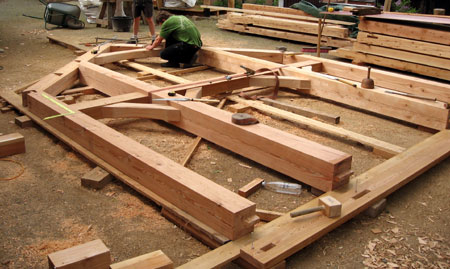
\includegraphics[width=0.99\textwidth]{images/01/Fachwerk_Abbund.jpg}
    \caption[Example of timber frame components being assembled on the ground]
    {Example of timber frame components being assembled on the ground \\
        \footnotesize{(Credits: CC AS 4.0 Licence photo by Georg Hefter - Traditionelles Fachwerk und Timberframe im Vergleich auf georghefter.de)}}
    \label{fig:example-timber-frame-on-ground}
\end{figure}

\subsubsection{Post and Beam Structure}
\label{subsubsection:introduction-post-and-beam-structure}

The third defining characteristic of timber frame construction is post-and-beam structural framing \parencite{jacksobonHistoricAmericanTimber2014,sobonTimberFrameConstruction1984}. The use of large timber sizes in timber frame structures allows them to be strong enough without the use of continuous load-bearing walls. The main benefit is the flexible arrangement of floors and walls to suit different architectural programmes. 
On the other hand, integral timber joints are generally weak in rotational stiffness, causing the joints to behave kinematically. Therefore, diagonal bracing is often introduced to fully or partially triangulate the structure to improve structural stiffness. Being limited by the joint design, these bracings function primarily in compression. It is, therefore, common to design the bracings in complementary pairs to resist dynamic wind loads coming from opposing directions. While some architectural designs may find the intrusion of diagonal bracings obtrusive to usable space, these diagonal bracings are highlighted on the facade as ornamentation in half timber designs \parencite{gernerFachwerkEntwicklungGefuege1979}. In this thesis, the demonstration structures are designed with similar structural principles, specifically the use of structural triangulation in the design offered unique stability advantages during the robotic construction process \seeref{subsection:exploration-4-deformation-awareness-and-error-correction-by-triangulation} \seeref{subsubsection:exploration-4-global-correction-approach}.

Figure \ref{fig:half-timber-frame-example} shows an example of a half-timber style timber frame house in Soest, Germany. Notice the exposed diagonal elements on the facade.

\begin{figure}
    \centering
    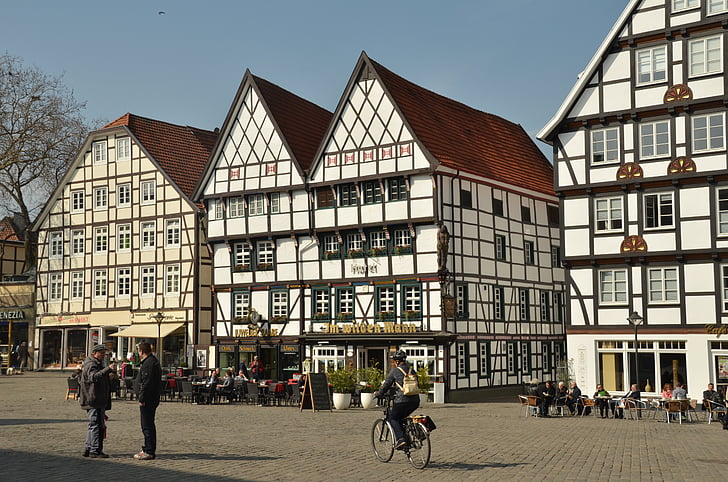
\includegraphics[width=0.99\textwidth]{images/01/germany-soest-architecture-timber-framed-preview.jpg}
    \caption[Example of a half-timber style timber frame house]
    {Example of a half-timber style timber frame house \\
        \footnotesize{(Credits: Licence-free photo, retrieved from \url{https://www.hippopx.com/en/germany-soest-architecture-timber-framed-half-timbered-house-square-city-402214} , n.d.)}}
    \label{fig:half-timber-frame-example}
\end{figure}


    
\subsection{Current Practice of Timber Frame Construction}
\label{subsection:introduction-current-practice-of-timber-frame-construction}

Timber frame construction was once the dominant building method, but it gradually declined in popularity during the 19\textsuperscript{th} and 20\textsuperscript{th} centuries. The advent of industrialization and mass production led to the availability of cheaper building materials such as steel and concrete, which were faster and easier to use. Even within the timber construction sector, newer construction methods that use dimensioned lumber, glulam, LVL, and Cross Laminated Timber (CLT) have replaced timber frame construction. However, in recent years, as more people are aware of the environmental benefits of wood construction, interest in timber frame construction is increasing again as an alternative way to construct with timber. 

Advancements in engineering and design, as well as increased availability of sustainably sourced timber, have helped to make timber frame construction a more viable option for modern building projects. Timber frame components can be prefabricated off-site, which can reduce construction time and costs while also minimising waste and environmental impact. The use of dry-fitted integral timber joints reduces the number of fasteners and components involved, meaning less metal consumption and quicker installation on-site. Furthermore, timber frame structures can be aesthetically pleasing as they often expose the beautiful timber material and reveal the structural load paths. When the joint details are exposed, they can evoke a feeling of tradition and craftsmanship and are often well-appreciated by those who inhabit the building.

\subsubsection{Automatic Machining of Timber Joints}
\label{subsubsection:introduction-automatic-machining-of-timber-joints}

Between the years of decline and its recent resurgence, a number of technological improvements have made timber frame construction more efficient and competitive. One of the major advancements has been the use of automatic joinery machines for carving integral timber joints. Traditionally crafted with hand tools, these joints were labour-intensive and required highly skilled craftsmen that could work precisely.\footnote{The task of marking and setting out was considered the most critical and is often performed by the master carpenter. Other carpenters would prepare materials and carve joints using hand tools such as saws, planes, chisels, and drills.}
Since the invention of automatic joinery machines, the production of timber joints has become highly automatic \parencite{hanshundeggeragCorporateDevelopment2023}. These machines often feature interchangeable cutting tools and can create many types of joints at the beam ends and along its length. Today, the machining of timber joints is very mature and efficient. The automatic joinery machines are controlled by Computer Numeric Control (CNC) technology and can follow a digital program to create timber joints of different designs at different positions. The program can be quickly changed to create different timber elements used for an entire building. \seeref{subsection:introduction-programming-digital-fabrication-machines}

This thesis capitalises on the accuracy and prefabrication efficiency provided by the automatic joinery machines. Accurate parts are highly advantageous for robotic automatic assembly because they ensure accurate manipulation and precise integration. By using prefabricated timber parts with accurately machined integral timber joints, this thesis aims to create a highly automated assembly process, reducing the manual labour needed for adjustment and adaptation. 

\subsubsection{Assembly by Carpenters}
\label{subsubsection:introduction-assembly-by-carpenters}

Although the production of timber frame components is automated, the assembly of the structure is still predominantly manual \parencite{willmannNewParadigmsAutomatic2016}. It usually takes a team of carpenters to assemble a timber structure.

Timber frame structures are almost always assembled on-site due to the nature of their post-and-beam structural system, which favours long and unbroken elements. This means that pre-assembling multiple elements off-site, is not practical because it will result in assemblies that are too big for transportation. 

Below is a summary of the tasks that carpenters perform during the assembly of a timber frame structure, focusing on the structural elements:

\begin{itemize}
	\item \textbf{Sorting timber parts --} Prefabricated timber parts are typically delivered on-site in bundles that correspond to different assembly stages. Many of the components are geometrically unique because of the layout of the joints. Carpenters must identify the correct location for each element based on label and markings on the parts and sort them according to the assembly sequence.

	\item \textbf{Manipulating timber parts spatially --} Post, beam and diagonal bracings are assembled in different spatial (3D) orientations. Carpenters must identify and orient the parts correctly when bringing them to their assembly location.

	\item \textbf{Applying forces --} Because of contact friction and deformation, carpenters may need to apply force to the joints using hand tools. They may use common generic tools such as mallets and screwdrivers (pulling with a screw), or specialise tools such as ratcheting joint pullers. 

	\item \textbf{Aligning mating joints --} Multiple carpenters are often required at every mating joint. They may have to push or pull the already-assembled elements for alignment. 

	\item \textbf{Synchronous Assembly --} During the closure of the joints, the carpenters also ensure parallel and synchronous motion to avoid jamming.

	\item \textbf{Adjusting timber joints --} If a timber part does not fit. Carpenters can remove material or shim gaps. These types of problems are rare with CNC fabricated parts, but can sometimes occur due to poor machining tolerance, design error, machine-programming error, and shrinkage or expansion after machining.

	\item \textbf{Placing fasteners --} Some contemporary joint designs include screws, nails, or dowels.

\end{itemize}

These tasks are the focus of the automated assembly process pursued in this thesis. The challenges of each task are analysed and presented in the next chapter \seeref{section:challenges-mechanical-challenges}.

\subsection{New Opportunities for Timber Frame Construction}
\label{subsection:introduction-new-opportunities-for-timber-frame-construction}

Compared to other newly developed construction methods with a higher degree of prefabrication, the on-site timber frame construction is less economically competitive. For example, modular floor and wall construction allow more components to be assembled off-site (e.g. insulation, windows, doors), which reduces the time and cost associated with on-site work. Volumetric prefabrication (e.g. modular timber construction), which pre-assembled an entire room, further allows the installation of wiring, plumbing, and interior finishes in a factory \parencite{adelDesignRoboticallyFabricated2018}. 

Despite the lack of prefabrication advantages, timber frame construction enjoys greater design freedom because there are fewer transportation constraints when moving linear timber elements than moving a preassembled room-sized timber module. This freedom is essential in creating large-span structures or shell structures where sub-assemblies cannot be effectively transported. In addition, latest timber frame designs have already been able to integrate contemporary building requirements such as plumbing, electrical wiring and insulation that meets building codes \parencite{bensonTimberframeHomeDesign1988}. Therefore, the exploration of automatic assembly for timber frame structures could potentially keep these benefits without the associated penalty of on-site manual work.

\section{Architectural Design to Production}
\label{section:introduction-architectural-design-to-production}

In recent years, the fields of architecture and construction have seen a growing interest in automating various stages of the design and production process. This trend is being driven by the potential benefits of automation, which include increased efficiency, higher precision, and improved quality control. Automation can also help to reduce labour costs, minimise waste, and improve safety on construction sites. While automation has already become common in the manufacturing industry, its adoption in architecture and construction has been slower due to the unique challenges and complexities in the construction sector. Most commercialised examples are limited to prefabrication of small or planar architectural components while only a handful of research projects have attempted to use robotics for structural scale spatial assembly. Therefore, this thesis aims to expand knowledge in this area, starting with the assembly of timber frame structures.

This section will present a brief history of how the timber construction industry transitioned towards digital design and automated production, leading to the current state of the art practices. It is an important starting point to understand whether the assembly process will also undergo such a transition. 

\subsection{Automation from Manufacturing to Construction}
\label{subsection:introduction-automation-from-manufacturing-to-construction}

The beginning of automation started with the manufacturing industry. It involves the use of machinery or computer systems to perform tasks that would otherwise be done by human labour. Without going into details, it typically involves the use of sensors, actuators and control systems to reduce or eliminate the need for human intervention \parencite{nofSpringerHandbookAutomation2009}. It has become a widely adopted practice in the manufacturing industry due to its benefits such as increased efficiency, improved quality, and reduced costs. With automation, the production process can run continuously with a predictable production schedule.

The successful implementation of automation is closely tied to the design and operation of production machines. Since the beginning of industrial automation, automatic machines have undergone several evolutions that are characterised by their features, modes of operations and benefits. Early automatic machines were mechanical systems that performed repetitive fixed operations. Their motions were often defined mechanically through the use of components such as linkages, cams and conveyor belts. Because of this, their motions cannot be easily modified without changing parts. These machines favour high-volume, low variability products that represent the mass-production paradigm of Industry 2.0\footnote{The First Industrial Revolution, aka. Industry 1.0, began in the late 18th century where mass production was carried out by machines powered by water and steam.}.
While some of the earlier machines still require an operator, later machines would contain control systems that are capable of performing cyclic actions on their own. After the introduction of electricity, the use of logic controllers became more common and allowed the machines to make decisions using sensors and signals. The increased level of autonomy allowed further reduction of operator interventions. This type of automation is a typical defining characteristic of Industry 3.0 \parencite{mengesNewCyberPhysicalMaking2015,yinEvolutionProductionSystems2018}. 

Invented in the 1950s and popularised in the 1960s, Computer Numeric Control (CNC) technology further increased the flexibility of machines, such as the aforementioned automatic joinery machines and industrial robotic arms. The motion of CNC machines are defined through the use of a digital ‘program’ such that their motion can be easily modified when products are changed \parencite{wardAutomaticProgrammingNumerically1959}. This is often achieved by incorporating a computerised digital control. The ability to change design quickly eventually led to the mass-customisation paradigm of Industry 4.0. In extreme cases, products can even be unique from piece to piece, resulting in the ‘batch size of one’ paradigm \parencite{wardAutomaticProgrammingNumerically1959}.

The adoption of automatic machines has changed the nature of work from labourers to operators and increasingly towards engineers and programmers \parencite{nobleForcesProductionSocial1986}. While this shift may be difficult for workers unable to acquire a new skill set, it improves the general labour working conditions in the longer term \parencite{stromquistWorldDevelopmentReport2019}. For example, by reducing repetitive manual tasks or avoiding working in dangerous environments. 

\paragraph{A Factory for Making Buildings}

\label{subsubsection:introduction-a-factory-for-making-buildings}

At a larger scale, the concept of automation can be applied to connect different machines together to autonomously regulate production flow. There are two types of connections involved, the first is physical connections, such as using conveyor belts and robotic arms to move parts between machines. The second is logical connections, such as programmable logic controllers forming complex logic networks. In extreme cases, the term \textit{lights-out factory} or \textit{automatic factory} was used to describe large production facilities that are able to sustain continuous production with very few or infrequent operator involvements \parencite{nobleForcesProductionSocial1986,walkerAutomaticFactoryCase1957}. 

Recently, the introduction of large-scale concrete 3D printing technology has brought the automatic factory vision within reach for the architecture and construction community \parencite{ngoAdditiveManufacturing3D2018}. While large-scale 3D printing processes are still at the research stage, smaller 3D printers have already achieved full autonomy, allowing users to press a start button and come back later for the completed parts. The idea of a black-box fabrication machine where design information and raw materials are the only input, was hypothesised to be the future mode of production that can make almost anything \parencite{gershenfeldHowMakeAlmost2012, gershenfeldInternetThings2004}.  

Started in the late 1970s, Japan’s large construction contractors have begun developing robots capable of performing construction tasks. The initial robots were single-task construction robots, designed to perform one specific function, such as finishing concrete, welding, or spray painting \parencite{potterJapanSkyscraperFactories2022}. Starting in the mid-1980s, Japan’s construction robot development shifted away from individual robots, and towards creating an entire robotic construction site \parencite{maedaCurrentResearchDevelopment2005}. The process often makes use of a high number of prefabricated components and focuses on improving the speed for the assembly task. Studies have found that the productivity gain is often apparent when constructing a tall and repetitive building \parencite{linnerAutomatedRoboticConstruction2013,potterJapanSkyscraperFactories2022}. 

While the automated systems seen in Japan are mostly designed for steel and reinforced concrete structures, this thesis studies what it would take for timber construction to achieve a similar level of automation. 

\subsection{Automatic Assembly in Timber Construction}
\label{subsection:introduction-automatic-assembly-in-timber-construction}

In recent years, interest in exploring automatic assembly for timber construction has grown. This was driven by the potential for increased efficiency, precision, and sustainability. Despite the advancements in fabrication techniques, particularly with the advent of CNC technology, the assembly process still presents challenges that industry professionals and researchers are working to address \parencite{willmannNewParadigmsAutomatic2016}.

In the industry, the advancement was mainly focused on the assembly of flat-stackable prefabricated parts, such as light-framed timber floors and walls. Companies like Biesse, Homag, and Weinmann have been developing advanced machinery and automated solutions for timber processing and assembly \parencite{kooTechnologyGapsAchieve2021}. These systems are often large-scale installations similar to a manufacturing production line and are custom engineered for a specific factory. The entire system can include separate material processing stations, such as cutting and joinery machines and for linear timber and panel saws for sheet materials. Processed materials would merge into a central assembly line and be assembled using nails, screws and adhesive depending on its design. Additionally, companies like MiTek and Randek have been focusing on the prefabricated housing sector, developing automated systems for the assembly of timber roof trusses \parencite{ianharveyRoboticArmsAI2018}. 

Despite these groundbreaking efforts, the challenges for spatial timber assembly is rather unique \seerefii{section:challenges-mechanical-challenges}{section:challenges-computational-and-design-challenges}. These challenges are complex, interdiscipline and are often specific to the construction system. This makes it hard to generalise solutions between different type of constructions. For example, despite having high demand in the industry, the spatial assembly of planar walls to create volumetric timber modules is still performed manually; timber frame structures, despite existing for a long time, still have no automatic assembly solutions. As the demand for sustainable building solutions continues to grow, and the skilled labour market continues to shrink, the exploration of automatic assembly methods for timber construction is urgently needed. 

Several innovative research projects have emerged in recent years, addressing the challenges of spatial manipulation of linear timber elements. For instance, the pioneering work conducted by Gramazio Kohler Research at ETH Zurich has shown the potential of using industrial robots to assemble complex timber structures. While early explorations were limited to a 2.5D stacked assembly approach \parencite{apolinarskaSequentialRoof2016, gramaziokohlerresearchethzurichStackedPavilion2009, helmInSituFabricationMobile2014}, many later projects addressed 3D spatial manipulation. For example, the first two-story robotically assembled structure \parencite{eversmannRoboticPrefabricationTimber2017}, the volumetric timber modules of the DFAB House \parencite{adelDesignRoboticallyFabricated2018, thomaRoboticFabricationBespoke2018}, and many other spatially assembled timber structures \parencite{apolinarskaRoboticAssemblyTimber2021, eversmannRoboticPrefabricationTimber2017, helmAdditiveRoboticFabrication2016, helmreichRoboticAssemblyModular2022,willmannNewParadigmsAutomatic2016}. Similarly, other research institutes have demonstrated the capabilities of using industrial robots to assemble prefabricated timber plates spatially \parencite{robellerRoboticIntegralAttachment2017, rogeauRoboticAssemblyIntegrallyAttached2023} and to assemble modular timber cassette systems \parencite{alvarezBUGAWoodPavilion2019, claypoolAutomationDiscreteExploring2021}.

This thesis aims to contribute to the ongoing efforts to advance the state of the art in this domain. Using timber frame construction as a starting point, the assembly problems are studied and addressed in a holistic way, with the intention to improve the understanding of these problems and for generalizable solutions to emerge.

\subsection{From Automation to Digital Fabrication}
\label{subsection:introduction-from-automation-to-digital-fabrication}

In the 1990s, various computer programmes that were intended for animation (e.g. Alias Wavefront, Maya) and engineering (e.g. Catia, later DigitalProject) were adopted by the architectural community for modelling geometrically complex buildings. This partially triggered the bloom of freeform architectural designs that are made famous by architects such as Frank Gehry, Zaha Hadid, Santiago Calatrava. For example, \textit{Fishdance Restaurant, Kobe (1989),  Guggenheim Museum Bilbao (1997), Walt Disney Concert Hall (2003)},and \textit{ Louis Vuitton Fondation (2014)}.\textit{ }

The immediate implication of freeform architectural designs is the need to produce geometrically complex components. This was addressed by the use of CNC machines that can follow arbitrarily complex paths. However, freeform architectural designs also implies the need to produce a large amount of non-repetitive components. At the component level, this is similar to the mass-customisation paradigm in manufacturing. However, in order to create the unique CNC programmes for the production process, Computer-aided design (CAD) and computer-aided manufacturing (CAM) software became an indispensable part of the production workflow \parencite{sheldenDigitalSurfaceRepresentation2002}. 

\textit{CAD software} allows architects and construction engineers to create 2D or 3D models of buildings, including the detailed geometry of each building component. Using these models, production engineers use \textit{CAM software} to generate toolpaths for the CNC machines. Because of the non-repetitive geometry, each component requires a unique programme for the CNC machines for operation and unique drawings for the workers to perform the assembly and inspection. This eventually leads to a workflow where not only are the machines automated, but the production of information is also automated. This new mode of production became what is known now as \textit{Digital Fabrication}.

The basic workflow for CAD is called direct modelling, where designers explicitly create and modify geometry in a linear workflow. This can be analogous to the ‘drawing’ process in architectural design as the designer interacts with the computer program over a graphical user interface (GUI) in an interactive way. The designer can use functions offered by the CAD to add or modify geometry. A more advanced workflow is \textit{parametric modelling}, where the history of modelling operation is saved for later reuse. This can be as simple as a ``Macro", where multiple functions are chained for easy access, or as complex as to define geometry based on a chain of functions and input parameters. This can be analogous to writing a mathematical equation with functions and variables. By changing the input values to the variables, the equation can be used to represent many possible outcomes. Therefore the output of a parametric model is dynamic and can be regenerated if necessary. Designers typically create a parametric model in one of the two ways. The first method is by demonstrating the modelling or computation logic to the CAD programme while the programme ‘records’ the logic which can be reused later. The second method is to create a symbolic description, similar to computer programming. This is often called \textit{Scripting} and is often used for more complex logic. Depending on the CAD programme, this symbolic script can be written in one of the many programming languages (e.g. C$\#$, Python) or, more recently, in a graphical programming interface (e.g. Grasshopper, Dynamo). 

There are two important benefits of a \textit{reusable CAD workflow}. The first is to save time when modelling large amounts of geometrically similar (but not identical) parts. The second benefit is the ease of making design changes. For example, the designer only needs to change the inputs for the CAD programmes to update the downstream documents automatically. These can include 3D models of components, 2D drawings and assembly instructions. In recent years, the popularity of parametric workflow has shaped the way designers interact with the design process. Instead of focusing on the final outcome, the automated workflows allow them to design the geometrical logic first before adjusting the input parameters to achieve the desired geometry \parencite{jabiParametricDesignArchitecture2013}. In addition, measurement and evaluation logic can also be incorporated into the script, allowing designers to be more informed about their designs. Complex relationships between geometry and structure can also be scripted to allow an intuitive and interactive design process \parencite{pottmannArchitecturalGeometry2007, woodburyElementsParametricDesign2010}. This design process that is supported by parametric modelling is often called \textit{Parametric Design}.

\subsection{Programming Digital Fabrication Machines}
\label{subsection:introduction-programming-digital-fabrication-machines}

Reusable workflows have also been extended to the CAM software to generate machining programmes automatically. This refers not only to the automated creation of toolpaths from a part geometry, but also the automatic decision-making to choose machining strategy, tool choice, machining sequence, and machining speeds. In the architectural context, this type of workflow has been used for cutting 1D profile materials and 2D sheet materials for geometrically complex facade systems used in free-form buildings \parencite{eigensatzPanelingArchitecturalFreeform2010, sheldenDigitalSurfaceRepresentation2002}.

In timber construction, the aforementioned automatic joinery machines were invented before the digital fabrication revolution \parencite{hanshundeggeragCorporateDevelopment2023}. Programming work for these machines was initially done by manually entering joint parameters (such as joint type, size and location on the beam). However, this work was soon automated by CAD (e.g. Cadwork 1988) and CAM (e.g. LignoCAM) software that was developed for the timber industry \parencite{schwinnManufacturingPerspectives2016}. Timber-specific CAD software improved efficiency for modelling matching pairs of joints across different elements and reduced the risk of design errors. While the CAM software is responsible for converting the joint features of the 3D model (such as cutouts and drill holes) into machine-specific programmes for the automatic joinery machines.

In the early days, CAD and CAM functionality were integrated into the same programme. However, as more machine manufacturers such as Biesse, SMC Group, and Homag started to make automatic joinery machines, open file formats were developed to allow different CAD, CAM and automatic joinery machines to work interchangeably. The current industry standard is the BTL (2006) and later BTLx (2015) format for data exchange. They were developed by a collaborative effort from the industry to create a specialised format for describing timber components. For example, it can represent timber grain directions, glulam orientation and joint machining tolerance that would otherwise not be possible using generic 3D model formats \parencite{lignocamBTLxWhatIt2020, design2machineHistoryDataTransfer2023}. 

The design-to-production workflow would typically start with a timber engineer that creates 3D models of the arrangement of beams and joints in the CAD software. Design iterations would happen within the CAD programme until architectural and structural requirements are met. Construction planning would also be performed in the CAD environment for specifying the production schedule and assembly sequence. The description of the beams and joints would then be passed to machine-specific CAM software by using, for example, the BTLx file format. The CAM programme would be able to recognise the timber elements and their joint details and make machining decisions specific to the fabrication machine setup. For example, to choose a suitable saw, mill bit or drill bit size from a collection of available tools; or to decide whether a hole is drilled or milled.

A production engineer, who has intimate knowledge of the machine setup, is often involved in defining the rules that the CAM software would follow. The ruleset would include a description of machine limitations, available tools, material choice, desired machining quality and production sequence. Conceptually, this is similar to the reusable CAM workflow mentioned above with a similar intention to automate the CAM software, to handle a large number of geometrically unique elements. 

Hypothetically, the assembly process studied in this thesis can also adopt a similar workflow. There is a strong similarity between creating machining programmes and creating robotic assembly programmes. Both of them are specific to the machine setup (e.g. robot kinematics), machine limitation (e.g. avoiding collisions) and tools setup (e.g. end effectors). It also needs to overcome the complexity of making decisions according to unique geometry. Therefore, this thesis adopts the parametric modelling and reusable workflow from machining as a starting point and apply it to robotic timber assembly \seeref{subsection:exploration-3-workflow-for-generating-assembly-programmes}. 

\subsection{Fabrication-aware Design}
\label{subsection:introduction-fabrication-aware-design}

\begin{quote}
	``While digital models are easily created, the actual fabrication and construction remain a challenge.'' \parencite{pottmannArchitecturalGeometryFabricationAware2013}
\end{quote}

The disconnection between design and fabrication is the source of numerous frustration that forced many geometrically complex projects into a ‘redesign’ phase after the reality of fabrication and construction limitations was imposed. This redesign process is known as rationalisation \parencite{pottmannArchitecturalGeometryFabricationAware2013}. A rationalisation is a design negotiation between keeping the design intent and reducing fabrication costs. It invariably led to a loss of fidelity. A better approach would be to incorporate knowledge of the actual construction process during the design stage; this is known as construction-aware or fabrication-aware design.

In the current architecture and construction industry, the role of evaluating constructability lies in the hand of a construction engineer. Very often it is a single-direction workflow that is difficult to accommodate frequent design changes. As architectural design practices migrate towards a digital workflow, there is a growing interest to automate the evaluation process. One common approach is to encode the knowledge of the fabrication constraints as computational algorithms, which can be computed automatically within the CAD design software. Feedback can therefore be provided as quickly as possible for the designers, which gives them a better chance of pushing designs closer to fabrication limits yet without violating them. 

These automatic checks, also known as design validation, are particularly useful when dealing with designs that have many unique parts (that would otherwise need to be checked individually) or when the fabrication limitations are complex or obscure. They also help avoid human errors and mistakes that are costly to fix downstream. 

While the concept of fabrication-aware is often used to check prefabricated components and machining processes, the concept can hypothetically be applied to a robotic assembly process. For example, robot reachability, payload, and collision. As long as a constraint can be modelled as a computable algorithm, it can be checked automatically. However, in practice, not all checks are easy to model and certain behaviour requires advanced simulation to model. This will be further elaborated in the next chapter \seeref{section:challenges-computational-and-design-challenges}. However, it is exactly because of this complexity that makes it difficult for a designer to evaluate them manually. Therefore in the context of this thesis, one of the main explorations is to study whether robotic assembly processes can be checked automatically and whether a fabrication-aware design workflow is feasible. 

The following sections present two case studies in the field of digital fabrication. They provided a positive indication that an integrated design and fabrication workflow is achievable.

\subsubsection{Case Study - Automatic CNC Machining Programme}
\label{subsubsection:introduction-case-study-automatic-cnc-machining-programme}

The first case study is a comparison between robotic assembly and machining processes. Assembly robots are similar to complex milling machines with multiple axes in the sense that they are both capable of making complex movements. However, they are also prone to programming errors that can cause expensive damage. Therefore, when creating toolpaths, a CNC programmer will often rely on the multitude of checking algorithms offered by the CAM software to catch potential problems. It is common for a CNC programmer to resolve production problems separately, within the scope of modifying machine parameters, tooling or cutting strategy. It is only until the attempts are exhausted that the programmer will suggest design changes to the designer. 

The culprit of this long evaluation cycle is that the current practice of creating toolpaths requires a lot of manual input. On the one hand, this offers many optimization possibilities for the machining process but at the same time makes feasibility evaluation very complex. In order to address this problem, researchers have identified the need to combine the automatic generation of toolpaths and automatic validation \parencite{garciaProcessPlanningBased2011,sheenMachiningFeatureRecognition2006, joshiGraphbasedHeuristicsRecognition1988}. These methods have already been adopted by companies offering machining services to generate CNC programmes automatically. This enabled them to provide almost-instant price quotations for parts solely based on a geometrical model. 

Similar to the hypothesis proposed before \seeref{subsection:introduction-programming-digital-fabrication-machines}, there are a lot of similarities between an assembly process and a machining process. Perhaps the same automatic generation and validation principle can be applied to robotic assembly processes to enable a more integrated workflow.


\subsubsection{Case Study - Automatic Slicing for 3D Printing}
\label{subsubsection:introduction-case-study-automatic-slicing-for-3d-printing}

Another parallel can be drawn between robotic assembly and additive manufacturing. Fused Deposition Modeling (FDM) Printers are mechanically simple devices that can create 3D parts by stacking 2D slices. However, the generation of toolpaths (a.k.a slicing) requires advanced algorithms to determine optimal toolpath, layer height, infill density, print speed, and other settings based on the geometry of the model, the type of printer, and the material being used. Additionally, the slicer software needs to take into account various non-linear factors that can affect the quality of the printed object, such as the cooling rate of the material, the shrinkage of the material as it cools, and the adhesion of the material to the print bed. Slicers may also include features such as support generation, which creates structures to support overhanging features of the model during printing. 

As a result, slicers can be quite complex and require a significant amount of tuning and customization. Nevertheless, pre-tuned slicers for commercially available printers can produce satisfactory results for almost any 3D geometry. In many cases, they are fully automatic upon the reception of a CAD model and do not require any manual input. When processing a problematic design, such as large overhangs, the software is able to pinpoint the problematic area for the designer to resolve. 

Similarly, robotic assembly processes also require complex software algorithms to model robot kinematics, tool behaviour, and environmental limitations. The fact that full automation can be achieved in slicer programs provides an optimistic indication that robotic assembly processes may achieve a similar degree of automation.

\section{Robotics in Architectural Assembly}
\label{section:introduction-robotics-in-architectural-assembly}

Robotics involves various disciplines that deal with the design, construction, operation, and use of industrial robots. The disciplines include mechanical engineering, electrical engineering, and computer science. Industrial robots play a crucial role in performing tasks autonomously or with minimal human intervention. There are many types of industrial robots, typically classified by their kinematic configurations, such as Cartesian Robots, Cylindrical Robots, and Articulated Robots \parencite{waldronKinematics2016}. Articulated robots, also known as robotic arms, are the most common type used for spatial manipulation. They typically contain 4 to 7 rotary joints (usually 6) arranged in a chain and connected by rigid metallic bodies. This allows spatial positioning and agile movements beyond orthogonal directions.

Robotic arms are multipurpose machines that can be used for material handling, machine tending, and performing assembly tasks when equipped with a task-specific tool. This tool is known as an end-effector. In the context of this thesis, the assembly task is the size of a building. In order to extend the reachable area of a robotic arm to cover the entire volume of the construction, a unique setup is used where a robotic arm is mounted inside a 3-axis overhead gantry\seeref{subsection:methodology-laboratory-context}, a configuration similar to the Japanese building factories.

Many research projects have already explored the adaptation of robotic arms to perform architectural assembly tasks \seeref{subsection:introduction-automatic-assembly-in-timber-construction}. However, the use of robotic arms in the construction industry presents unique challenges due to the non-repetitive nature of the tasks involved. The two main challenges relevant to this thesis are the inaccuracy of non-repetitive targets and the automation of planning non-repetitive trajectories.

\subsection{Inaccuracy for non-repetitive targets}
\label{subsection:introduction-inaccuracy-for-non-repetitive-targets}

Most of the industrial robotic arms available in the market today were designed for the manufacturing industry. Their long kinematic chains are designed to be able to reach into tight spaces such as machine openings and car interiors. For this purpose, agile motions are preferred over mechanical stiffness and accuracy. In the context of manufacturing, robotic tasks are often repetitive, targets and payload are also known in advance during programming. As long as the robot repeatability is good, manual calibration can be performed to achieve good alignment, this is known as Teaching \seeref{subsection:exploration-3-robot-targets-taught-configuration-and-cartesian-pose} \parencite{shohamRobotTeachingMethods1984}.

However, the difference between repeatability and accuracy is important to consider when using robotic arms for non-repetitive tasks. Repeatability refers to the robot's ability to return to a specific position with high precision, while accuracy is a measurement of the robot's ability to reach a previously uncalibrated target position. This is much more challenging for the robot to achieve because it needs to take into account discrepancies in the robot kinematics model, manufacturing tolerance of the robot parts, and deformation of the robot under different payloads and configurations. 

While the kinematic model of a robot can be calibrated \parencite{mooringFundamentalsManipulatorCalibration1991}, the changing deformation due to payload and configuration is hard to predict. Formally, this is the difference between open-loop (repeatability) and close-loop (accuracy) control concerning the end-effector poses. At the moment, most of the industrial robots on the market (including the one used in this thesis) are only close-loop controlled until the joint positions. The end-effector pose is open-loop controlled.  

Using robotic arms for architectural assembly typically entails a large number of unique targets. However, manually teaching each unique target would defeat the purpose of automation. Therefore, the practical limitation of this inaccuracy is studied in this thesis. For example, how it affects the timber frame assembly process, what are the associated failure modes, how does it affect failure rate and what strategies can be used to mitigate the problem. For the sake of clarity, it should also be pointed out that redesigning a robotic arm is beyond the scope of this thesis.

\subsection{Automation for planning non-repetitive trajectories}
\label{subsection:introduction-automation-for-planning-non-repetitive-trajectories}

The anatomy of a robot program can be seen as a segment of movements that goes from one target to the next. The trajectory is simply a matter of interpolating between different targets. However in reality, there are many limitations to this interpolation. For example, some robotic joints cannot be rotated through 360 degrees between interpolation, or if the interpolation results in a collision.

In industrial automation, the production engineer will typically teach waypoints for the robot to move around obstacles. Once the teaching is completed, the engineer will also verify the motion at a slow speed to ensure it is collision-free and later at higher speed (production speed) to ensure dynamic effects are acceptable. Although this process of teaching and validation is tedious and time-consuming, it is acceptable for a repetitive process, because it has to be done only once. 

Alternatively, the configurations and associated trajectories can also be created in a computer simulation, using algorithms that are referred to as motion planners\parencite{lavallePlanningAlgorithms2006}. This workflow requires all the objects and machines around the robot being modelled in the simulated environment for collision checking \seeref{subsection:exploration-2-motion-planning}. Even so, small adjustments may be required in the physical environment as the alignment between physical setups and their simulated counterpart may differ significantly.

For planning non-repetitive trajectories the impracticality of teaching the targets means that simulated motion planning must be used. Therefore it will suffer from the accuracy problem when alignment is needed with real world objects. Moreover, the construction environment must be accurately modelled and cannot be changed during the robot operations. 

% \chapter{Challenges and Research Goals}
\label{chapter:challenges_and_research_goals}

State of the art in automatic joinery machines and its design-to-CNC workflows have indicated that the technical bottleneck to prefabricate unique timber parts have long been solved. The entire production workflow from CAD design to joinery fabrication have already been digitised and automated. The next research frontier is to automate the assembly of the components into a complete structure. Using timber frame structures with integral timber joints as a starting target, this thesis aims to explore the roadblocks that are still in the way of automatic spatial timber assembly. The goal is to better understand existing challenges, discover new problems, identify possible solutions, develop new models and pave the way for future in-depth research.

The general research question is ``\textbf{How can robots assemble spatial timber structures}?". However, the formulation of more specific questions is treated as a product of first understanding precedence works and their challenges. This approach allows for a more focused study on the commonly encountered problems and to steer towards generalizable solutions while avoiding common culprits. Therefore, this chapter will start by presenting the known challenges related to the automatic assembly of spatial timber structures before summarising on the more detailed research questions that are pursued in the rest of the thesis. This chapter consists of the following parts: 

\textbf{Section 2.1 Mechanical Challenges }focuses on the mechanical tasks that are physically performed during the construction. It represents the fabrication part of the ``Digital Fabrication" paradigm - the automation of the production tasks.

\textbf{Section 2.2 Computation and Design Challenges} presents the computational problems required to prepare the information for the robotic process. In particular, the automatic and human-in-the-loop workflows to create robotic programmes from a design. It represents the digital part of the ``Digital Fabrication" paradigm - the automation of the production of digital information.

Finally, research questions are formulated in \textbf{Section 2.3 Research Questions}. 

\section{Mechanical Challenges}
\label{section:challenges_mechanical_challenges}

\subsection{Sliding Friction}
\label{subsection:challenges_sliding_friction}

During the closure of a timber joint, surfaces between each pair of joints start to make contact. Apart from butt joints\footnote{ Definition of butt joints for this thesis are joints that do not have rubbing contact surfaces. Contact force only appears when the beam reaches its final, assembled position}, most of the joints are designed with a substantial amount of contact surfaces that will slide and rub against each other during assembly. The diagram below shows the increasing amount of rubbing surfaces in a pair of half lap joints during assembly. 

\begin{figure}
     \centering
     \begin{subfigure}[b]{0.32\textwidth}
         \centering
         \includegraphics[width=\textwidth]{example-image-a}
         \caption{Sub figure caption}
         %\label{fig:unique_subfigure_label}
     \end{subfigure}
     \hfill
     \begin{subfigure}[b]{0.32\textwidth}
         \centering
         \includegraphics[width=\textwidth]{example-image-b}
         \caption{Sub figure caption}
         %\label{fig:unique_subfigure_label}
     \end{subfigure}
     \hfill
     \begin{subfigure}[b]{0.32\textwidth}
         \centering
         \includegraphics[width=\textwidth]{example-image-c}
         \caption{Sub figure caption}
         %\label{fig:unique_subfigure_label}
     \end{subfigure}
        \caption{Figure Caption}
        %\label{fig:unique_figure_label}
\end{figure}


The design of these contact surfaces are used for many different purposes. For example to introduce geometrical interlock \parencite{larssonTsugiteInteractiveDesign2020, songRecursiveInterlockingPuzzles2012}, improve load transfer \parencite{likosEffectTenonGeometry2012}, improve structural stiffness \parencite{fangJoineryConnectionsTimber2018} or to improve stability against live load \parencite{jacksobonHistoricAmericanTimber2014}. Depending on the geometry of the sliding surface (e.g. tapered vs parallel) and the quality of the machined surface (e.g. rough vs smooth surface) these rubbing surfaces introduce different amounts of sliding friction that must be overcome by force.

Carpenters have always been aware of the quality of the joints and how it affects the assembly difficulty. However, with the use of CNC controlled joinery machines, the fabrication tolerance can be controlled much more easily. It is worth mentioning that one precedent project has attempted to control the moisture of the wood to shrink it for reducing friction \parencite{jennyPedagogyDigitalMateriality2022}. However the approach required heating the entire piece of wood, and would be difficult for larger scale structures.

\subsection{Tight Fitting Joints}
\label{subsection:challenges_tight_fitting_joints}

The second form of assembly-resistance is the fit of the mating joints. Fit is a measurement of the tightness of the connection between two mating parts. The fit can be categorised into three main types: clearance fit, transition fit, and interference fit. Clearance fit allows for some play between the parts, whereas interference fit requires force to assemble the parts and creates a tight, secure connection. Transition fit lies between these two extremes, providing a snug fit with some allowance for slight variations in the parts' dimensions.

Various factors can influence the fit of the mating joints, such as machining tolerances \parencite{thibautWoodMachiningFocus2016}, movement of the timber after machining due to release of stress, and environmental conditions such as temperature and humidity change {(Cochran, 2018)}\parencite{cochranTimberFrameLayout2018}. 

Tighter fits can result in higher frictional forces, which may require more force to overcome during assembly. It can also increase the difficulty for the robot to align the joints to begin assembly, which may increase the failure rate. Conversely, looser fits can lead to lower frictional forces but may compromise the structural integrity or performance of the assembled components \parencite{robellerRoboticIntegralAttachment2017}.

Existing studies on the effects of timber joint fit are mostly focused on furniture scale joinery using hardwood and with glue. \parencite{elekEvaluationEffectOptimal2020, koerner-al-rawiRoboticTimberAssembly2020, larssonTsugiteInteractiveDesign2020, likosEffectTenonGeometry2012} At the scale of timber frame construction, the choice of fit is typically based on the carpenter's experiences and historically proven norms \parencite{chappellTimberFramerWorkshop2011}. Only one recent study reported on the force required for architectural scale timber joints for plate structures \parencite{robellerRoboticIntegralAttachment2017}. 

In fact, much of the architectural scale robotic assembly research avoided the problem of tight fitting joinery at all due to the difficulty in assembling them, instead they use tangential connections \parencite{apolinarskaSequentialRoof2016, gandiaAutomaticPathPlanning2018, paraschoCooperativeRoboticAssembly2019}, and butt joints \parencite{apolinarskaRoboticAssemblyTimber2021, thomaRoboticFabricationBespoke2018} that did not require a large assembly force. However, these joint designs require an extra fastening step, such as glueing \parencite{gramaziokohlerresearchethzurichSemiramis2022, helmreichRoboticAssemblyModular2022} and screwing \parencite{apolinarskaSequentialRoof2016, thomaRoboticFabricationBespoke2018} that is often performed manually. Even when integral timber joinery was involved, a loose fit was chosen to make the robotic assembly process easier. 

\subsection{Assembly Force vs Robots}
\label{subsection:challenges_assembly_force_vs_robots}

The need to apply a large assembly force to overcome sliding friction and tight fit is a challenging problem for robotic assembly. 

Industrial robots, with their long kinematic chains are good for agile motions and spatial manipulation but are not optimal for applying large assembly force, typical industrial robots have payload capacity under 300kg, which roughly translates to 3kN of force. This is no match even against a reasonably tight timber joint at architectural scale. Even for special robots (e.g. palletizing and foundry robots) where the payload carrying capacity is high, they are bulky and heavy and are difficult to be integrated with a larger gantry system for architectural scale operation. 

The second challenging reason is that the large assembly force has to be applied directly on the mating joints. Considering that the most reasonable way for a robotic arm to hold a piece of timber would be from the middle, near its centre of gravity, the holding position would unlikely be where the joints are. For example, if a beam has two mating joints on the two ends, the pushing forces from the robotic arm would have to transfer through the length of the beam, by bending it, before it reaches the joints. Considering the low stiffness of the material, even if the robotic arm is strong enough, the strong pushing force would result in substantial bending or even damaging the beam. 

The third challenging reason is that there are more than one mating joint to be closed when assembling a beam. It is well known that the assembly of all the joints must proceed synchronously, or else the beam would jam and get stuck \parencite{dupontJammingWedgingConstrained1994}. Therefore, even if a robot could push from the centre of the beam without damaging it, any slight imbalance in the joint resistance among mating joints would result in a large torque on the wrist of the robotic arm. If the robot used a stiff control, this would likely result in an overload. If the robot used a compliant control, the beam would start to rotate and quickly get stuck. 

The fourth challenging reason is that a strong pushing force requires an equally strong reaction force that can support the other side of the mating joint. Therefore, even if a super robotic arm would be possible and the timber beam is not jamming, it is impossible to guarantee that the supporting force can be transmitted from the ground through the partially assembled timber structure without damaging what has already been built. The only possible alternative is to engineer a special end-effector to provide both the pushing force and the support at the same time, similar to the configuration of a clamp or a parallel gripper.

The fifth challenging reason is that the location and amount of timber frame joints can vary substantially between different elements in a timber frame structure. In addition, the shape of the joints are also variable, depending on the intersecting angles between the beams. Therefore even if a clamping end-effector concept is used, it is difficult to design it to accommodate different joint locations and joint angles. A severe limitation in the design possibilities would likely defeat the purpose of using robots to assemble structures in the first place. Perhaps this end-effector method would be possible for special cases where the joints are always at a similar location. For example, certain space frames with a topologically repetitive arrangement \parencite{apolinarskaRoboticAssemblyTimber2021, willmannNewParadigmsAutomatic2016}. 

An alternative approach that was considered is to use more than one robotic arm, each holding a clamping end effector near the joints. However, it is challenging to scale up for more complex arrangements as the number of robots will have to increase with the number of simultaneously assembled joints. While this may be possible for a two-robot scenario, more robots will simply not fit in the limited space between them.

\subsection{Joint Alignment}
\label{subsection:challenges_joint_alignment}

During the assembly of timber structures, it is necessary to accurately align the mating joints between the robot-sode and the stationary-side.

On the robot-side, the joints are located on the beam that is being held by the robot. Because these beams have to be assembled in non-repetitive targets, teaching cannot be used \seeref{subsection:introduction_inaccuracy_for_non_repetitive_targets}. Therefore the end-effector that holds the beam is subjected to unmonitored deviation. If the timber elements are long, a small orientation error can cause a large positional deviation at the joints that are located far away from the robot wrist. Furthermore, long timber elements may also be slightly bent (permanent and static) or deflect (dynamic) due to its own weight, which further increases the deviation at the location where the joints mate.

On the stationary-side, the joints are spread across different elements in the partially constructed structure. Due to accumulated installation error, or deformation of the flexible timber structure, the location of the joints can deviate from where they are supposed to be. Moreover, the deviation among each of the joints may not be towards the same directions, making detection and correction difficult.

Because the robot targets are all extracted from a CAD model, unless there are active sensors monitoring the location of the joints on both sides, the joint pairs are likely to be subjected to misalignments which cannot be detected or corrected. Even if the misalignment can be detected, if there are more than one joint to align, correction may still be impossible due to conflicting deviation direction.

In the case where misalignment is severe and the problem is undetected, the subsequent robotic motion will not only fail but can also damage the timber parts. 

\subsection{Fastener Installation}
\label{subsection:challenges_fastener_installation}

While many of the traditional timber frame joints contain no fasteners, some of them do, and for a multitude of reasons. For example, timber wedges are used to pull the joints tighter during assembly and can improve its stiffness; Timber dowels or pegs are used to prevent joint loosening due to live load; Metal dowels are used in contemporary designs to transmit shear force with metal plate connectors; Metal screws can be used to transmit tensile forces over a joint that would be hard to achieve using timber contact faces alone. 

The assembly of threaded fasteners is a common operation in the manufacturing industry \parencite{jiaSurveyAutomatedThreaded2019}. Many different types of specialised end-effectors, robotic screwdrivers and screw feeding systems are designed to accommodate different types of screws. In timber construction, the automated assembly lines for prefabricated light-timber frame walls often have integrated screwdrivers and nail guns. Automated nailing has also been demonstrated for large-scale architectural construction \parencite{apolinarskaComplexTimberStructures2018, apolinarskaSequentialRoof2016}. However, most of these systems have been used for assembling planar assemblies and there are extra challenges when this has to be performed spatially. For example, handling long screws and non-orthogonal entry angles. Many of these precedence projects have resorted to assembling the screws manually \parencite{apolinarskaRoboticAssemblyTimber2021, thomaRoboticFabricationBespoke2018, willmannNewParadigmsAutomatic2016}. 

For timber frame construction with larger timber sizes, the screws used on the integral timber joints are often much larger than those used in the lighter timber systems. For other fasteners such as dowels and wedges, they are more specialised and have no automated precedence. 

\section{Computational and Design Challenges}
\label{section:challenges_computational_and_design_challenges}

\subsection{Designing with Integral Timber Joints}
\label{subsection:challenges_designing_with_integral_timber_joints}

Timber frame structures often employ the use of integral timber joints that are interlocking, to restrict the movement of beams after assembly. In many cases, there is only one single direction in which the mating beams can be moved to assemble the joints. The arrangement of beams and the design of the interlocking joints works together to provide the stability and stiffness of a timber frame structure. However, this approach also creates a complex, interlocking system of parts that are difficult to design and analyse, not unlike the 3D interlocking puzzles commonly found in museum gift shops.

Carpenters have long understood that a successful timber structure is not only one that stands up, but also one that can be assembled. In the pre-digital era, the scale and complexity of large timber structures, such as pagodas, roofs, and bridges, required the most experienced master carpenters to design \parencite{haymanTimberframedBuildings2021, hewettEnglishHistoricCarpentry2022, mullerHistoryDevelopmentStages2022, vandenabeeleJoiningTechniquesNineteenth2018}. Even today, one of the most challenging tasks when designing a complex timber structure is to ensure that the beams and their joints satisfy both structural and assembly requirements \parencite{chiltonTimberGridshellsArchitecture2016}.

\begin{itemize}
	\item Structural requirements include arranging beams into a stable and functional structural system and designing the joints to transmit structural forces. 

	\item Assembly requirements include ensuring that all components can be manoeuvred into place, accounting for the constraints imposed by the interlocking joints, and verifying that the assembly sequence does not create conflicts or blockages \parencite{wangStateArtComputational2021}. 

\end{itemize}
Historically, successful timber frame designs were passed from one generation of carpenters to the next, each of them making iterative improvements. Particularly successful designs, such as post-and-beam structures and long-span roof trusses became a typology that was repeated and used many times \parencite{sobonTimberFrameConstruction1984, jacksobonHistoricAmericanTimber2014}.

Today, advances in the computer graphic field have created many analytical methods and opened up new possibilities for designing and analysing novel timber structures. In this thesis, structural analysis and assembly analysis will not be the core focus of the research. This is because they are already a highly established field and that many existing works have already studied them in depth. However, it is still necessary to be aware of their challenges to be able to apply the techniques correctly.

\subsection{Structural Analysis}
\label{subsection:challenges_structural_analysis}

Timber structures are designed by considering various factors such as material properties, structural loads, environmental conditions, building codes, and aesthetics. The process typically begins with architectural design, where the overall form and layout of the building are determined. This is followed by structural design, where the appropriate sizes and shapes of timber members, connections, and joints are selected to ensure structural integrity, stability, and longevity.

Timber structures, particularly those with integral timber joints, present unique challenges in terms of analysis due to the complexity of the joint behaviour, material properties, and load distribution. These challenges can make it difficult to accurately predict the structural performance and ensure the safety and longevity of the structure. Some of the key challenges in analysing integral timber joints are:

\begin{itemize}
	\item \textbf{Anisotropic material properties --} The mechanical properties of wood material vary along different directions. This anisotropy can affect the behaviour of integral joints, as the strength and stiffness of the joint depend on the direction of the applied loads and the orientation of the wood fibres. Accurate analysis must account for these variations in material properties \parencite{thelanderssonTimberEngineering2003}.

	\item \textbf{Non-linear behaviour --} The behaviour of timber material and timber joints can be non-linear, particularly under high load levels or in the presence of defects, such as cracks or knots. This non-linear behaviour can complicate the analysis process, as it requires more advanced numerical methods and computational models to accurately predict joint performance \parencite{gustafssonFracturePerpendicularGrain2003, tanadiniAnalysisDesignTimbertotimber2021}.

	\item \textbf{Moisture content and hygroscopicity --} Wood is hygroscopic, meaning it absorbs and releases moisture in response to changes in environmental conditions. This can cause dimensional changes and affect the mechanical properties of the timber, impacting the behaviour of integral joints. Accurate analysis must account for these moisture-related effects and their potential impact on joint performance \parencite{thelanderssonTimberEngineering2003}.

	\item \textbf{Load distribution and interaction --} Integral timber joints often involve complex load distribution and interaction between multiple components. This can make it difficult to accurately predict the load-carrying capacity and failure modes of the joint. Advanced structural analysis techniques, such as finite element analysis (FEA), are often required to accurately model these interactions and predict joint behaviour .

	\item \textbf{Uncertainty in material properties and geometric tolerances --} Variability in material properties, such as strength and stiffness, as well as uncertainties in geometric tolerances, can make it challenging to predict the behaviour of integral timber joints with high confidence. Probabilistic approaches, such as reliability analysis \parencite{ranta-maunusReliabilityAnalysisTimber2001} and stochastic finite element methods \parencite{kandlerStochasticFiniteElement2015}, can be used to quantify these uncertainties and assess the impact on joint performance.

\end{itemize}
\subsection{Assembly Analysis}
\label{subsection:challenges_assembly_analysis}

Assembly analysis of timber frame structures with integral timber joints is a crucial aspect to ensuring the structure can be assembled, this is known as joint mobility analysis, or assemblability analysis. The assembly analysis can be extended to include automatic sequence planning and motion planning \parencite{wangStateArtComputational2021}. Assembly problems can be further categorised \parencite{wangStateArtComputational2021} by their properties: 

\begin{itemize}
	\item \textbf{Number of hands --} number of simultaneously moving parts needed for assembly 

	\item \textbf{Monotonicity --} whether the parts can be assembled in one simple motion, or whether intermediate movements are needed.

	\item \textbf{Linearity --} whether the assembly motions are linear, rotational, helical or other freeform motions. 

\end{itemize}
Most of the precedence robotic assembly projects in the architectural field, including the timber frame assembly problem in this thesis, belong to the simplest option of all (single hand, linear and monotonic movements). Even for projects that have used more than one robot during the process \parencite{paraschoCooperativeRoboticAssembly2019, thomaRoboticFabricationBespoke2018}, unless it involves multiple simultaneous movements in different trajectories, they are still considered one-hand problems.


Large amount of research has been devoted to the automatic sequence and motion planning. For example, in the context of mechanical assembly \parencite{bahubalendruniReviewAssemblySequence2016, defazioSimplifiedGenerationAll1987, homemdemelloTaskSequencePlanning1989, wilsonGeometricAssemblyPlanning1992b}, computer graphics \parencite{natarajanPlanningAssemblies1988, wangDESIAGeneralFramework2018} and also timber construction \parencite{taiDesignAssemblyComputational2012}. It is also possible to include additional heuristics in the search of an optimal assembly plan. For example, to maximise structural stability during construction \parencite{deussAssemblingSelfsupportingStructures2014, garrettScalableProbabilisticallyComplete2020}, avoid robotic collision \parencite{huangFrameFabRoboticFabrication2016, yuHighlyInformedRobotic2016} or to minimise assembly time.

When robots are used to perform an assembly task, the assembly analysis mentioned above also has to consider the actions of the robots and the tools, and their physical limitations. These limitations include

\begin{itemize}
    \item \textbf{Collision --} The robot and parts attached to the robot must not come into collision among itself or with stationary objects \seeref{subsubsection:exploration_2_collision_checking}.

	\item \textbf{Reachability --} The robot must be able to reach all the targets that are needed to manipulate the objects for their assembly \seeref{subsubsection:exploration_2_inverse_kinematics}.

	\item \textbf{Payload and Accuracy --} Certain operations may not be possible due to the mechanical limitations of the robot.
\end{itemize}

The extension of these analysis into the design process includes:

\begin{itemize}
	\item \textbf{Automatic Sequence Planning --} Identical to the sequence planning above, concerned with the sequence among parts.

	\item \textbf{Automatic Task Planning --} Planning the discrete actions of the robot to assemble each part (e.g. open gripper, move, close gripper, etc.) \parencite{homemdemelloTaskSequencePlanning1989}

	\item \textbf{Automatic Motion Planning --} Finding the trajectory for the robot joint to follow, such that the attached end-effector moves from one target to another. \parencite{lavallePlanningAlgorithms2006}
\end{itemize}

In this thesis, task planning and motion planning are unavoidable for generating the robot programmes. However, sequence planning will not be studied. It is assumed that an experienced timber engineer, designer or carpenter can be tasked to determine the assembly order based on experience and intuition.

\subsection{Task and Motion planning}
\label{subsection:challenges_task_motion_planning}

The use of robots for assembling timber structures requires careful planning and simulation to ensure that there are no unintended collisions. 

The basic task of picking up a beam carrying it to the assembly location may sound simple for a human worker. However, the planning work required for a robot to do the same is not only computationally hard, but also complicated to set up correctly. The parameters that have to be planned are:

\begin{itemize}
	\item \textbf{Tasks --} What are the sequence of operations for moving the robot joints and actuating the attached tools (e.g. opening and closing grippers)?

	\item \textbf{Grasp --} What pose (position and orientation) does the robot use to hold the beam? Does the robot need to change its grasp during the process?

	\item \textbf{Targets --} Where are the targets for the robot to reach at the start and end of a motion to pick or place a workpiece at the correct location.

	\item \textbf{Trajectories --} What is the continuous path (a series of static joint angles) that allows the robot and its attached objects to move from one target to the next?

\end{itemize}
The main challenge for spatial assembly is that there are many possible directions and orientation for assembling an element. This is in steep contrast to a layer-by-layer construction approach, where new elements can be assembled from the top \parencite{apolinarskaSequentialRoof2016, gramaziokohlerresearchethzurichStackedPavilion2009}. 

Many spatial assembly projects have used a rule-based strategy to programme the transfer path. For example, a common approach for beam transfer is to raise the beam to a safe height before traversing horizontally \parencite{hackStructuralStayinplaceFormwork2020, sondergaardTopologyOptimizationRobotic2016}. However, this approach is still limited by the obstacles at the final approach when the robot is near the partially-assembled structure. For structures that are assembled from the core towards the periphery, a strategy of approaching the target from the ‘outside’ can be used \parencite{adelDesignRoboticallyFabricated2018}. 

A more generic strategy is to use a sampling-based motion planner as it has the ability to automatically search for a viable path while avoiding collisions \parencite{gandiaAutomaticPathPlanning2018, thomaRoboticFabricationBespoke2018}. This is critical if some of the beams have to reach into the small openings of a structure. However, one of the often cited knowledge gap remains at the automatic generation of robotic trajectories for large amounts of uniquely shaped and positioned elements \parencite{eversmannRoboticPrefabricationTimber2017, gandiaAutomaticPathPlanning2018}. Latest research developments have already created the interface to access planning tools from the robotics research field for planning architectural assemblies \parencite{gandiaAutomaticPathPlanning2018, paraschoCooperativeFabricationSpatial2017a, paraschoComputationalDesignRobotically2018}. The most comprehensive method to date being a unified sequence and motion planning or a unified task and 

\subsection{Joint Modeling and Solving}
\label{subsection:challenges_joint_modeling_solving}

Joint Modeling and Solving refers to the computational process of creating and adjusting parametric models of integral timber joints, ensuring their compatibility and adaptability within the larger context of the timber frame assembly, while taking into account fabrication constraints, user customizations, and structural considerations.

Timber joints are typically modelled as a subtraction from the beam’s geometry. In many joint designs, both halves of the joints are not geometrically similar, therefore the subtraction geometries for the beams on each sides are also different. In order to ensure correct fit, it is necessary to ensure that both sides of the joint will match with each other. While this is relatively straightforward to achieve for one joint instance, a parametric joint model will need to adapt itself to different jointing angles between the beams. Because of the continuous nature of the joining angles, the model requires defining parametric geometrical relationships in 3D to create the solid models \parencite{vestartasDesigntoFabricationWorkflowRawSawnTimber2021}. In general, a parametric joint model will contain fixed properties that are dependent on the neighbouring beams, and editable properties that can be customised:

\textbf{Adaptation to the intersecting beams' position, size and angle --} This adaptability allows the joint geometry to be computed automatically by the intersecting beams without explicit modelling. Thus, changing the intersecting beams’ locations can trigger an update to snap it to a new position. The images below shows a mortise and tenon joint adapting to different beam intersection angles.

\begin{figure}[H]
    \centering
    \includegraphics[width=\textwidth]{example-image-a}
\end{figure}

\textbf{Customization of detail sizes or proportions - }Even a simple lap joint model can include an adjustable parameter for the cheek depth. More complex joint topology can have many adjustable parameters. \textit{(refer to the diagram of a housed dovetail T Lap having many parameters) }These adjustments are often useful for changing the structural behaviour of the joint and may be specified or changed at a later stage of the design process during engineering calculations. The images below show a mortise and tenon joint having the same intersection angles but different topologies. The proportion of the details in each topology would require a parametric definition.

\begin{figure}[H]
    \centering
    \includegraphics[width=\textwidth]{example-image-a}
\end{figure}

Different ways to parametrise a joint model can result in different behaviour during size and angle adaptations. The choice of parameterization affects not only the structural behaviour of the joint but also the range of which a joint model can deform before it becomes invalid. For example, an intersection angle adaptation may result in an undercut geometry that cannot be cut with an automatic joinery machine.

Therefore it is common to consider the fabrication process and its constraints when creating a parametric joint model \parencite{vestartasDesigntoFabricationWorkflowRawSawnTimber2021}. Some joint designs are even dependent on the shape of the cutting tool. For example, the dovetail joint in the images below (left) is created by a dovetail milling cutter (below image, right). In those scenarios, it is necessary to contact the fabricator for a list of possible joint feature dimensions. 

% 2 Horizontal Image  
\begin{figure}
    \centering
    \begin{subfigure}[b]{0.49\textwidth}
        \centering
        \includegraphics[width=\textwidth]{example-image-a}
        \caption{Sub figure caption}
        %\label{fig:unique_subfigure_label}
    \end{subfigure}
    \hfill
    \begin{subfigure}[b]{0.49\textwidth}
        \centering
        \includegraphics[width=\textwidth]{example-image-b}
        \caption{Sub figure caption}
        %\label{fig:unique_subfigure_label}
    \end{subfigure}
    \caption{Figure Caption}
    %\label{fig:unique_figure_label}
\end{figure}


\footnotesize Photo by Hannes Plackner \parencite{HightechDovetails2014}

Parametric joint models can be categorised according to what beam intersection topology it can adapt to. For example, side-side, side-end, and end-end types \parencite{vestartasJoinerySolverWhole2020}This grouping allows automatic determination of what parametric model can be used for a given beam intersection type. In addition, the grouping can also include the assembly direction of the beams relative to each other. For example, the images below show assembly direction (red) being perpendicular to the beam axis (a and b) and parallel to the beam axis (c).

% 3 Horizontal Image  
\begin{figure}
     \centering
     \begin{subfigure}[b]{0.32\textwidth}
         \centering
         \includegraphics[width=\textwidth]{example-image-a}
         \caption{Sub figure caption}
         %\label{fig:unique_subfigure_label}
     \end{subfigure}
     \hfill
     \begin{subfigure}[b]{0.32\textwidth}
         \centering
         \includegraphics[width=\textwidth]{example-image-b}
         \caption{Sub figure caption}
         %\label{fig:unique_subfigure_label}
     \end{subfigure}
     \hfill
     \begin{subfigure}[b]{0.32\textwidth}
         \centering
         \includegraphics[width=\textwidth]{example-image-c}
         \caption{Sub figure caption}
         %\label{fig:unique_subfigure_label}
     \end{subfigure}
     \caption{Figure Caption}
     %\label{fig:unique_figure_label}
\end{figure}




It is worth noting that the solution space for a timber joint is large, and there are no existing approaches for evaluating all these requirements. Therefore, even though the solving process can theoretically be automatic, in practice, it often starts with the designer’s intuition and is later checked by the various design checks mentioned before. 

While the automatic modelling of timber joints is not an essential requirement for automatic assembly, it is important for a parametric design process. Even in a simple structure, there are many joints involved. The sheer number of joints makes the process tedious and prone to human error if they are modelled manually. Furthermore, the inclusion of assembly direction in a parametric joint model allows automatic design check for assemblability. It can also be used for generating the robotic assembly program, because the assembly direction defines one of the important movement targets for that specific beam. 

\subsection{User Interface for Fabrication Aware Design}
\label{subsection:challenges_user_interface_for_fabrication_aware_design}

Creating designs in a highly constrained environment is often a balance between finding interesting possibilities while pushing the design boundary. Considering the many constraints, introduced in the previous sections, that are relevant to a robotically assembled timber frame structure, it is not hard to imagine the complexity of the design process. 

The computational approach to address these highly constrained problems is to use a powerful computer to search for valid solutions that could satisfy the given boundary conditions \parencite{pottmannArchitecturalGeometryFabricationAware2013, tamFabricationawareStructuralOptimisation2018}. In theory, as long as a constraint can be committed to computer code, it can be evaluated automatically. However, this technique is only meaningful for problems where the design space and the constraints are well defined \parencite{huangFrameFabRoboticFabrication2016}. In the case of architectural design, where the design space is infinite and the aesthetics of the structure is impossible to codify, the total exclusion of a designer is not meaningful. 

The alternative is a human-computer collaborative design process, or computer-aided design (CAD) in its essence, to combine the best of both agents. In this case, the human-computer interface (HCI), in the form of a graphical-user interface (GUI), becomes critical for successful collaboration of the two \parencite{preeceInteractionDesignHumancomputer2015}. 

The primary goal for such an interface is to provide designers with real-time feedback and guidance while allowing them to explore the design space and make informed decisions \parencite{frichMappingLandscapeCreativity2019, puentesMakingGesturesDesign2015}. This involves visualising and communicating various constraints, warnings, and possible solutions through a well-designed interface that is both intuitive and user-friendly. To achieve this, the interface for designing a robotically-assemble timber structure should consider the following features: 

\begin{itemize}
	\item \textbf{Interactive 3D visualisation --} Enables navigation of the model over each assembly step for the human designer to understand temporal and spatial relationships between the beams, joints and robots.

	\item \textbf{Constraint visualisation --} Visualise constraint violations and fabrication limitations. 

	\item \textbf{Solution suggestions --} Offers ways to address constraint issues and improve the design.

	\item \textbf{Integrated robotic assembly planning --} Seamlessly incorporates assembly feasibility within the design environment.

	\item \textbf{Interactive parametric modelling workflow --} Facilitates quick iterations between different solutions when solving problems.

\end{itemize}
In summary, a user interface for fabrication-aware design should facilitate effective communication between the human designer and the computational tools, enabling a seamless and efficient design process. 

\section{Research Questions}
\label{section:research_questions}

The challenges elaborated in the previous sections have indicated the highly interdisciplinary nature of this research. It includes the field of timber frame design, digital fabrication, machine design, computer graphics and robotics. Consequently, research questions that address these challenges require an integrated approach that combines expertise from these diverse fields..

Due to the novelty of the combination of the robotic assembly and integral timber joints, the thesis will adopt an exploratory research method (details in \textbf{Chapter 3 Methodology and Assumptions}). In this regard, the questions are open-ended and serve as a guide for exploration. 

\begin{enumerate}
	\item \textbf{What technologies (hardware and software) are required?}

    \begin{enumerate}
    	\item What are the \textbf{robotic end effectors} needed to assemble the joints? Can they be general purpose or specific to the type of joint being assembled?
    
    	\item Is the \textbf{accuracy of a typical industrial robot }sufficient to assemble beams with joints? Is it necessary to develop \textbf{sense, alignment and compensation }methods to overcome misalignment?
    
    	\item How suitable is an industrial robotic arm for performing spatial timber assembly? How can they be designed differently if they are optimised for construction purposes? How many robots are needed to assemble a building?
    
    	\item How can \textbf{computational tools }support a robotic assembly process? Can \textbf{robotic programmes be generated automatically} based on assembly design?
    
    \end{enumerate}
    
    \item \textbf{How will architectural design workflow and detailing have to change?}

    \begin{enumerate}
    	\item Will timber frame structures and integral timber joints be designed differently to accommodate the robotic process? For example, by adding \textbf{new details }to the beams and joints to \textbf{improve ease of assembly}? Can existing timber joinery machines produce these details?
    
    	\item How will the design process be different with the added constraints of robotic assembly? How will \textbf{design validation }be performed?
    
    	\item Who are the \textbf{new domain experts responsible for an automated construction process}? How can they participate in a design workflow?
    
    \end{enumerate}
    
    \item What are the \textbf{possible implications if robots assemble timber buildings in the future?}
    
    \begin{enumerate}
    	\item Existing robots are generally not as agile as human workers. Will robotic assembly limit the \textbf{architectural and structural design possibilities}?
    
    	\item How will \textbf{humans participate} in the transition to robotic construction? How will traditional roles such as carpenters change? What are the new roles that may emerge?
    
    \end{enumerate}
\end{enumerate}


% \chapter{Methodology and Assumptions}
\label{chapter:methodology-and-assumptions}

In this thesis, an exploratory research method was used. The first reason is the qualitative nature of the three research questions. The second reason is the novelty of the interdisciplinary topics which have yet to be studied in depth. The exploratory research consists of the following steps:

\begin{enumerate}
	\item \textbf{Identifying Challenges and Creating a Hypothetical Solution --} Although precedence works have already identified challenges in each subtopic \seerefii{section:challenges-mechanical-challenges}{section:challenges-computational-and-design-challenges}, a holistic analysis is still needed as certain challenges that are coupled together \seeref{subsection:exploration-1-analysing-assembly-challenges}. This leads to a hypothetical robotic assembly process that is based on the idea of a robotic arm manipulating and collaborating with a set of robotic clamps \seeref{subsection:exploration-1-distributed-robotic-tool-approach}.

	\item \textbf{Testing, observing and refining the Hypothetical Solution --} Technical development is performed, and their behaviour is observed with empirical experiments. A number of iterations is performed to refine the hypothetical robotic assembly process and to better understand the problems involved \seeref{section:methodology-research-by-iterative-development}.

	\item \textbf{Formulating relationships --} Critical analysis is performed during the development in each iteration and at the end of the thesis to answer the research questions and to provide possible avenues for future in-depth studies \seeref{section:methodology-epistemological-assumptions}.

\end{enumerate}
\section{Research by Iterative Development}
\label{section:methodology-research-by-iterative-development}

The most important part of this exploratory research is the emphasis on system development and hands-on empirical trial runs to refine the hypothetical solution for automatic assembly. Five distinct development rounds were conducted, each containing their own research goals, technical developments, experiments and observations \seeref{subsection:methodology-setting-research-goals}. The following flowchart summarises the iterative loops across the development rounds. 

% 1 Image  
\begin{figure}
    \centering
    \includegraphics[width=0.99\textwidth]{example-image-a}
    \caption{Figure Caption}
    %\label{fig:unique-figure-label}
\end{figure}

Within each \textbf{Development Phase}, small scale tests were performed and the technology was improved until it was ready for a full systematic test \seeref{subsection:methodology-technology-development}. 

The full full systematic test was performed by designing and constructing a \textbf{Demonstrator Structure} \seeref{subsection:methodology-demonstraror-design}. 

During the \textbf{Construction Phase}, certain adjustments of the process parameters are also possible. Afterwhich, the follow-up actions are determined for the next exploration round \seeref{subsection:methodology-observations-and-interpretation}.

\subsection{Setting Research Goals}
\label{subsection:methodology-setting-research-goals}

At the beginning of the first iteration, the goal was to design and prototype an assembly process and to test it with experiments. As new insights and discoveries are made, subsequent development iterations are guided by the discoveries and include follow-up explorations whenever necessary. Below is a summary of the goals in each phase:

\begin{itemize}
    
    \item \textbf{Exploration Round 1 - Clamp Prototype --} A minimal demonstration of the robotic clamp concept is developed to verify the process. The hardware being developed is only capable of assembling one type of lap joints with fixed dimensions. Nevertheless, it successfully performed the task and revealed opportunities for further improvements. \textit{(link to Chapter \ul{4 Exploration Round 1 - Clamp Prototype)}}
    
    \item \textbf{Exploration Round 2 - Bus Stop Demonstrator --} The initial proof-of-concept clamp is redesigned to accommodate joints with different angles. Software is also developed to generate robot trajectory, control the robot arm, and control the robotic clamps wirelessly. Finally, a high level controller is developed to synchronise motion between the robotic arm and robotic clamps - an important aspect of the assembly process. The entire system was validated through the construction of a timber frame structure with 40 elements. \textit{(link to Chapter \ul{5 Exploration Round 2 - Bus Stop Demonstrator)}}
    
    \item \textbf{Exploration Round 3 - Automatic Clamp Placement --} This phase completes the automation for mechanical tasks that are identified as low priority in the previous two phases. One of the highlights is the automatic placement and retrieval of robotic clamps on the structure. In addition, task planning and motion planning algorithms were introduced to study the automation of parsing designs to create robotic assembly programmes. The completed fully automatic assembly system was validated by reassembling the last demonstrator in a fully automatic manner.  \textit{(link to Chapter \ul{6 Exploration Round 3 - Automatic Clamp Placement)}}
 
    \item \textbf{Exploration Round 4 - HyparHut Demonstrator --} This phase consists of a UI upgrade to improve interactive modelling in the CAD environment, the introduction of a fabrication-aware design workflow, and the introduction of a new robotic screwdriver. The new screwdriver allows the assembly of non-planar lap joints and can accommodate timber beams with different profile sizes. This vastly expands the design possibilities for timber frame structures that can be assembled by the automatic process. The new system was validated with the assembly of a structure with a hyperbolic paraboloid roof. One other highlight was the introduction of a vision based alignment process for improving the success rate for the robotic arm to pick up and place tools. \textit{(link to Chapter \ul{7 Exploration Round 4 - HyparHut) }}
    \item \textbf{Exploration Round 5 - CantiBox Demonstrator --} By this round, the robotic assembly process had already achieved a high degree of automation and required little human intervention. The study was therefore expanded to integrate cutting-edge design methods with collaborators in two different fields. The first is structurally-informed joint design using novel design methods that is based on the theory of plasticity. This allows individually customised joints to respond to local load conditions. The main challenge on my part was to negotiate the intersection between assembly limitations, CNC machining limitations and structural optimization. The second is automated task and motion planning using PDDLStream to optimise redundant tasks and robotic motions. The main challenge is to formulate actions that can be understood by the computer algorithm to plan automatically. The combined technology was validated with the assembly of a structure with three modular boxes, each containing clamped and screwed joints. This also saw the largest amount of tools being used by the robotic assembly process, which provided insight for the future of the system. \textit{(link to Chapter \ul{8 Exploration Round 5 - Cantibox)}}
 
\end{itemize}
\subsection{Technology Development}
\label{subsection:methodology-technology-development}

The robotic assembly process required the development of novel hardware and software that form systems and subsystems that are interdependent in their operations. Below is an overview of the development categories showing their multidisciplinary nature. The software tools that are used for their development are listed in the bracket. 

\begin{itemize}
	\item \textbf{Mechatronics}

    \begin{itemize}
    	\item Robotic arm attachment hardware design (Rhinoceros 3D) 
    
    	\item Robotic clamp and screwdriver hardware design (Rhinoceros 3D) 
    
    	\item Robotic clamp and screwdriver electronics design (EAGLE)
    
    	\item Other static hardware supporting construction (Rhinoceros 3D) 
    
    \end{itemize}
    
	\item \textbf{Software for CAD}

    \begin{itemize}
    	\item CAD library for modelling timber parts and their assembly (Python)
    
    	\item Design validation tools (Python)
    
    	\item User Interface (UI) for interactive design modelling and validation (Python in Rhinoceros 3D) 
    
    	\item CAM library for modelling robotic tools and their actions (Python)
    
    \end{itemize}
    
    \item \textbf{Software for CAM}

    \begin{itemize}
    	\item Interface with task and motion planning software (Python) \textit{(footnote: in collaboration with YiJiang Huang)}
    
    \end{itemize}
    
     \item \textbf{Software for control and execution}

    \begin{itemize}
    	\item Robotic clamp and screwdriver firmware (C++)
    
    	\item Wireless communication firmware (C++)
    
    	\item Robotic arm and robotic tools synchronisation controller (Python, ROS)
    
    	\item Task execution and process monitoring software (Python)
    
    \end{itemize}
\end{itemize}

During development, multiple technical solutions can often be used to achieve a particular goal. The principle for selecting a specific option included the following criteria: 

\begin{enumerate}
	\item The cost of implementation is reasonable in the architectural construction context, and testing costs can be afforded by the given research budget.

	\item The implementation can be tested and observed within our laboratory.

	\item Software and hardware dependency is open source.

	\item The implementation is potentially generalisable. (e.g. a tool that can assemble more types of joints)

	\item The implementation is compatible with existing industrial practices or norms. (e.g. working with existing construction-grade tolerance instead of demanding a car-component-like accuracy) 

\end{enumerate}
Given the complexity of the AEC industry and its tendency to resist systematic changes, these principles guided the research direction towards finding implementable solutions with high impact.

\subsection{Demonstrator Design}
\label{subsection:methodology-demonstraror-design}

At the end of development phase 2, 4 and 5, the developed assembly process was observed and evaluated by the construction of a prototype structure. This is often called a demonstrator in the field of digital fabrication research. In total, there were three real-scale (1-to-1) demonstrators designed for this thesis. For the purpose of technical evaluation, the use of real-scale experiments revealed issues that were otherwise not observable in a computer simulation or a small-scale test. From the perspective of architectural design, the demonstrators served as a design study that can be experienced in person. Because of the high material cost and long preparation time required to construct such a demonstrator, each of them serves multiple investigation purposes to maximise the knowledge that can be extracted. Below is a list of design guidelines used when designing the demonstrators:

\begin{enumerate}
	\item The structure can be constructed with the developed system.

	\item The structure fits within our laboratory.

	\item The structure can demonstrate the flexibility of the assembly system (e.g. different types of joints, different joint angles, different element sizes, and different numbers of elements).

	\item The structures should present various difficulties for the assembly system (e.g. assembling very long elements, reaching into a congested space, joints very close to the ground or very high, many simultaneously assembled joints).

	\item The structures should contain various types of load-bearing elements (e.g. columns, floor beams, joists, diagonal bracings, rafters).

\end{enumerate}
During the design and preparation of the demonstrator, the newly developed CAD software (data structures, algorithms and user interfaces) was observed when it was used to model and encode the design. Flexibility and usability was observed first hand by the author, and improvements are sometimes implemented within the same development phase. The CAM software for translating design to robotic trajectories and execution programs was also tested. The result of this software is validated by performing digital checks such as robot kinematic simulation to catch collision problems. These problems must be fixed before the design phase can be concluded and timber parts can be ordered from the fabricator. 

During the demonstrator construction (also called Robotic Execution), the mechatronics hardware and control software was observed. The observation includes the dynamic behaviour when assembling different joint geometry and beam sizes at different orientations and with different support conditions. These observations provided evidence to identify key factors that limit system performance.  In addition, real world effects (such as gravity, material and robot inaccuracy) were observed during the assembly process to better understand fabrication constraints. This was used to improve the accuracy of automatic design checks for the fabrication-aware workflow.

Finally, the productivity of the robotic process was also observed by studying the time distribution during execution. While the exact duration in a laboratory condition may not correspond to an industrial automation scenario, it can reveal process bottlenecks and suggest possible improvements. Finally, unplanned manual interventions, such as robotic collisions, and overload errors due to jamming, are recorded and analysed qualitatively to identify patterns.

The timber parts used for the demonstrators were ordered from an industrial timber fabricator. Ordering from industry was preferred over creating the components within our laboratories because it allows a reality check of whether the newly developed digital workflow and timber details are compatible with the existing upstream industry. We have identified a single company (Auer Holzbau, Switzerland) to provide all the machining services in favour of consistency. The machining was performed on a recently released automatic joinery machine model (ROBOT-Drive 1250) manufactured by Hans Hundegger AG, Germany. The transfer of timber geometrical data is based on a proprietary file format of Cadwork (version 28). This is because the timber machining industry in Switzerland accepts it as a de facto standard for contractual agreement on the geometry of parts.

\subsection{Observations and Interpretation}
\label{subsection:methodology-observations-and-interpretation}

The \textbf{observations }made during the preparation and the execution of the demonstrators are documented as objectively as possible for each development phase (from Chapters 6 to 10). Based on these observations, \textbf{interpretations }are made to explain success and failure and are subsequently used to determine \textbf{follow-up actions}. Readers should be aware of the possible subjectivity in the interpretations and follow-up actions \seerefii{section:methodology-epistemological-assumptions}{section:methodology-axiological-assumptions}. 

% 1 Image  
\begin{figure}
    \centering
    \includegraphics[width=0.99\textwidth]{example-image-a}
    \caption{Figure Caption}
    %\label{fig:unique-figure-label}
\end{figure}

The diagram above shows different types of follow-up actions. For example, an observation may suggest new technology developments to improve the robotic assembly system. In some cases, further studies may be necessary to verify a causal relationship where the interpretations may be inconclusive. This can be caused by the scarcity of observations or the lack of scientific controls. Some other problems may require a design solution rather than a technological one, which can be addressed by formulating design guidelines or by creating automatic design checks. 

Note that some of the follow-up actions, such as adjusting software and tuning operation parameters, can be performed within the same exploration round. On the other hand, during the construction phase, the prefabricated timber parts cannot be modified easily and issues related to the demonstrator design can only be addressed in the next iteration. In addition, mechatronic and hardware issues often require substantially longer time to resolve. These problems were mostly addressed in the next round. 

Finally, follow-up actions are implemented wherever appropriate as long as my skills, research time and budget allow. Otherwise, the problems are elaborated for future investigations. 

\section{Epistemological assumptions}
\label{section:methodology-epistemological-assumptions}

The aim of the research is to create knowledge by developing, integrating and observing the effects of various technologies and the decisions made when designing the demonstration structure.

\textbf{Success and Failure} were evaluated based on whether the observed technology supports the vision of automatic design-to-assembly for timber frame structures. While some of the evaluation metrics are quantitative, others are qualitative such as when studying the generalizability and limitations of a particular technology.

\textbf{Causal Relationships} were established by logical reasoning, discussion with domain experts (e.g. CNC operator, Robot Technician, Structural Engineer, Architect) or quantitative experiments (e.g. tuning operation parameters, substituting parts or subsystems). The specific method to identify relationships was selected individually depending on the nature of the inquiry.

\section{Axiological assumptions}
\label{section:methodology-axiological-assumptions}

This thesis followed interpretivism principles, and many of this research's components are qualitatively analysed. Readers should therefore be aware of the author’s (my) background and its potential influence on the interpretation of data. In the rest of the thesis, first-person pronouns (i.e. I, my) are used as an indication of when decisions and interpretations are likely to be influenced by my background. Passive voice will continue to be used to describe objective observations and when making qualitative analyses.

\subsection{Researcher Background}
\label{subsection:methodology-researcher-background}

I was trained at the undergraduate and graduate levels as an architectural designer specialising in computational design. I have also practised mechatronics design in art and design, albeit without formal training. These experiences greatly influence my characterisation of the research questions as a technology development problem focusing on mechatronics and computational design instead of other pathways. For example, another researcher with a timber engineering background may approach the problem by proposing novel wood joints, or a roboticist may propose a novel control method for robotic manipulators. Nevertheless, mechatronics and computational design are the most common approach taken by many recent research projects, as introduced in the previous chapters.

\subsection{Laboratory Context}
\label{subsection:methodology-laboratory-context}

The research is conducted in the Robotic Fabrication Lab (RFL) of the Institute of Technology in Architecture (ITA) at the Department of Architecture of ETH Zurich, where four industrial robotic arms are mounted upside-down on two gantry robots (custom design by Güdel Group AG, Switzerland), forming a robotic manipulator that covers a large space \seeref{subsection:exploration-2-rfl-robotic-platform}. Each robot consists of six articulated joints, an independent vertical linear axis, and two horizontal linear axes on the gantry coupled with neighbouring robots. If only a single robot is concerned, all nine axes can be commanded to move synchronously. This offers kinematic redundancy that allows the robot body to avoid obstacles in dense environments. For this thesis, the robotic manipulator in the RFL represents a hypothetical robotic manipulator that acted as a testbed for developing the robotic assembly process. This also carries the assumption that lessons learnt from this setup can be extrapolated to on-site setups in the future. The details of this extrapolation are further discussed in the conclusion chapter \seeref{subsection:extrapolation-to-on-site-robots}. 

Our laboratory is also the home to many timber assembly research projects introduced in the context. This undoubtedly influences the research as existing robotic components and software infrastructure are adopted from previous research. For example, the choice of the automatic robotic quick-change system was the result of a donation from previous projects \seeref{subsection:exploration-2-docking-adapter}. Another example is the choice of online robot control middleware \seeref{subsection:exploration-2-distributed-control-system}, which was determined by our laboratory's standard mode of operations.

\subsection{Participants in User Interface Study}
\label{subsection:methodology-participants-in-user-interface-study}

While the user interface consists of only a small portion of the development work, it is interesting to observe how designers can use the newly developed design interface. In order to gather a bigger picture, participants (other than myself) are invited to design two of the three demonstrators. During the design sessions, which often span multiple weeks, I offered technical guidance to the designer and observed what knowledge I explicitly communicated to the participant. This mitigates some of my subjectivity when considering implicit versus explicit knowledge, especially because I am the main developer of both software and hardware systems. 

\section{Collaborations}
\label{section:methodology-collaborations}

Throughout this thesis, I collaborated with domain experts for some technological developments outside of my skills and knowledge. Their expert knowledge about state of the art in their respective fields helped me formulate the initial hypothetical solution. 

\begin{itemize}
	\item \textbf{Structural Analysis and Timber Joint Design }problems were advised by Dr. Davide Tanadini (Chair of Structural Design, ETH Zurich). His research focuses on possible applications of the theory of plasticity and graphic statics on timber structures and joints and their implementation in digital fabrication. In particular, the last demonstrator was designed by a student under his supervision (global design) and the joints were customised by the models and software he developed as part of this thesis. His PhD dissertation is titled ``Limit analysis and timber plasticity. Plastic design of interlocking timber-to-timber connections" \textit{(cite: Davides thesis) }Together with this thesis, they form part of the NCCR Digital Fabrication research project ‘Spatial Timber Assemblies’.

	\item \textbf{Robotic Task and Motion Planning (TAMP) }problems were advised by Dr. Yijiang Huang (Digital Structures Research Group, MIT, USA). His introduction and advice to the field was essential for me to understand the nature of the complicated problems involved. We worked in close collaboration for realising the three demonstrators, which led to the discovery of many new techniques to bridge between the highly technical fields (robotics and computer algorithms) and architectural design. Many of the planning related software, including all of the motion planning backend were developed by him. His PhD dissertation is titled ``Algorithmic planning for robotic assembly of building structures," \parencite{huangAlgorithmicPlanningRobotic2022}. Both of our researches share the same vision towards improving automation from design to assembly. 

	\item \textbf{Machine Design and Construction}, especially the later development with the screwdriver were advised by Prof. Dr. Agathe Koller and Marco Rossi (both from The Institute for Lab Automation and Mechatronics ILT, OST, Switzerland). They were directly involved in the conceptualization of the screwdriver operation mechanism and the innovative pin gripper mechanism. Marco also offered valuable instructions for machine design and construction, made some of the hardware parts and advised on the tests during hardware development

\end{itemize}
\section{Thematic Reading Guide}
\label{section:methodology-thematic-reading-guide}

The following five chapters (chapter 4 to 8) are written in chronological order corresponding to five development rounds. This is important for understanding the exploration as an evolution between experiments and observations.  Each chapter contains the following sections:

\begin{itemize}
    % 
	\item \textbf{Goal --} Identify the goal and scope for the entire exploration round

	\item \textbf{Background --} Background knowledge needed to understand the rationale for some of the development.

	\item \textbf{Development --} Technical description of the developed hardware and software. Some topics include the tests that were performed during development.

	\item \textbf{Lesson Learnt --} Observations, findings and interpretations related to the robotic construction demonstration. Some topics include hypotheses of possible cause(s), possible solution(s) and the follow-up action(s) taken. 

Readers who are interested only in a specific theme may find the following guide helpful for identifying a specific section. Note that this list is not exhaustive. 

	\item \textbf{Distribute Robotic Tools (DiRT) assembly method}

\begin{itemize}
	\item \textbf{Initial working hypothesis} of the DiRT clamps assembly method \seeref{subsection:exploration-1-dirt-clamping-assembly-process-task-list-v1}

	\item \textbf{Operation method revised} after initial test \seeref{subsection:exploration-3-dirt-clamping-assembly-process-task-list-v2}

	\item \textbf{Operation method with screwdrivers} \seeref{subsection:exploration-4-flowchart-for-screwdriver-assembly}

	\item \textbf{Operation method with clamps and screwdrivers }\seeref{subsection:exploration-5-combined-operation-of-clamps-and-screwdrivers}

	\item \textbf{Generalised operation principle} \seeref{section:discussion-generalised-dirt-system}

\end{itemize}
	\item \textbf{Two Types of DiRT Assembly Tools}

\begin{itemize}

	\item \textbf{Clamp }for planar lap joints

    \begin{itemize}
    	\item Hardware \seeref{subsection:exploration-2-lap-clamp-cl3-hardware}
    	\item Electronics \seeref{subsection:exploration-2-cl3-clamp-electronics}
    	\item Firmware \seeref{subsection:exploration-2-cl3-firmware}
    \end{itemize}
    \item \textbf{Screwdriver }for planar and non-planar lap joints 

\begin{itemize}
	\item Hardware \seeref{subsection:exploration-4-lap-screwdriver-sl1-and-sl1-g200-hardware}

	\item Electronics \seeref{subsection:exploration-4-sl1-screwdriver-electronics}

	\item Firmware \seeref{subsection:exploration-4-screwdriver-firmware-l1-control}

\end{itemize}
\end{itemize}
	\item \textbf{Other DiRT supporting hardware}

\begin{itemize}
	\item \textbf{Radio} \seeref{subsection:exploration-2-radio-network}

	\item \textbf{Gripper}

\begin{itemize}
	\item Short Parallel Gripper \seeref{subsection:exploration-2-parallel-gripper-pg500-and-pg1000}

	\item Long Parallel Gripper \seeref{subsection:exploration-4-parallel-gripper-pg1500-for-long-beams}

	\item Pin Gripper on Screwdriver \seeref{subsection:exploration-4-pin-gripper-mechanism}

\end{itemize}
	\item \textbf{Docking Adapter}

\begin{itemize}
	\item \seeref{subsection:exploration-4-docking-adapter-lock-sensor}

\end{itemize}
	\item \textbf{Camera Alignment System}

\begin{itemize}
	\item \seeref{subsection:exploration-4-camera-marker-alignment-correction-system}

	\item \seeref{subsection:exploration-4-camera-marker-hardware-on-docking-adapter}

	\item \seeref{subsection:exploration-5-camera-marker-hardware-on-cl3-clamp}

	\item \seeref{subsubsection:exploration-4-visual-guided-docking-process}

\end{itemize}
\end{itemize}
	\item \textbf{Design Software and Workflow}

\begin{itemize}
	\item \textbf{Design and Modeling Frontend}

\begin{itemize}
	\item \textbf{Design UI in Rhino Grasshopper} \seeref{subsection:exploration-2-cad-cam-user-interface}

	\item \textbf{Design UI (revised) in Rhino Python } \seeref{subsection:exploration-3-design-software-implementation-in-rhino-python}

	\item \textbf{Process Design Visualization} \seeref{subsubsection:exploration-3-process-visualization-and-adjustment}

\end{itemize}
	\item \textbf{Backend}

\begin{itemize}
	\item \textbf{Assembly Model} \seeref{subsection:exploration-2-assembly-model-data-structure-and-functions}

	\item \textbf{Process Model} \seeref{subsection:exploration-3-process-design-workflow}

\end{itemize}
	\item \textbf{Conceptual}

\begin{itemize}
	\item \seeref{subsection:exploration-4-deformation-awareness-and-error-correction-by-triangulation}

	\item \seeref{subsubsection:exploration-4-global-correction-approach}

\end{itemize}
\end{itemize}
\end{itemize}

\begin{itemize}
	\item \textbf{Task and Motion Planning }workflow \seeref{subsection:exploration-3-process-design-workflow}

\begin{itemize}
	\item \textbf{Narrow Passage Problem } \seeref{subsection:exploration-2-narrow-passage-problem}

	\item \textbf{Fast Check by IK} \seeref{subsection:exploration-4-fast-design-validation-with-ik-check}

	\item \textbf{Fast Check by LMG Planning} \seeref{subsection:exploration-4-planning-order-by-motion-group}

	\item \textbf{Non-sequential MMMP Solver} \seeref{subsection:exploration-3-taught-configuration-for-repetitive-targets}

\end{itemize}
	\item \textbf{Three Demonstration Structures Constructed}

\begin{itemize}
	\item \textbf{BusStop }Pavilion \seeref{subsection:exploration-2-demonstrator-design-busstop-pavilion}

	\item \textbf{HyparHut }Pavilion \seeref{subsection:exploration-4-demonstrator-design-hyparhut-pavilion}

	\item \textbf{CantiBox }Pavilion \seeref{subsection:exploration-5-demonstrator-design-cantibox-pavilion}

\end{itemize}
\end{itemize}

% \chapter{Exploration Round 1}
\label{chapter:exploration-round-1}

\section{Goal}
\label{section:exploration-1-goal}

The goal of the first round of development was to analyse the challenges related to the robotic assembly of timber frame structures and to propose a hypothetical solution that can address them \seeref{subsection:exploration-1-distributed-robotic-tool-approach}. Similar to the concept of a minimum viable product (MVP) in the field of product development, only the most critical component in the system was developed \seeref{subsection:exploration-1-scope-for-initial-exploration-round}.

\subsection{Analysing Assembly Challenges}
\label{subsection:exploration-1-analysing-assembly-challenges}

\todo{I have rewritten this paragraph and removed the table that was confusing.}
I started the exploration round by analysing the assembly challenges introduced in the previous chapter, Table \ref{table:response-to-challenges} shows a summary of the problems and my interpretation of their cause. It was evident that some of the problems, such as the low stiffness of timber material, could not be solved easily. Similarly, the tightness and rotational stiffness of timber joints are hard to control because they are sensitive to small changes in the joint cutting quality and material imperfections. My approach is to identify the problems that are solvable to derive actionable streategies for the development of robotic assembly tools.

\begin{table}[p]
    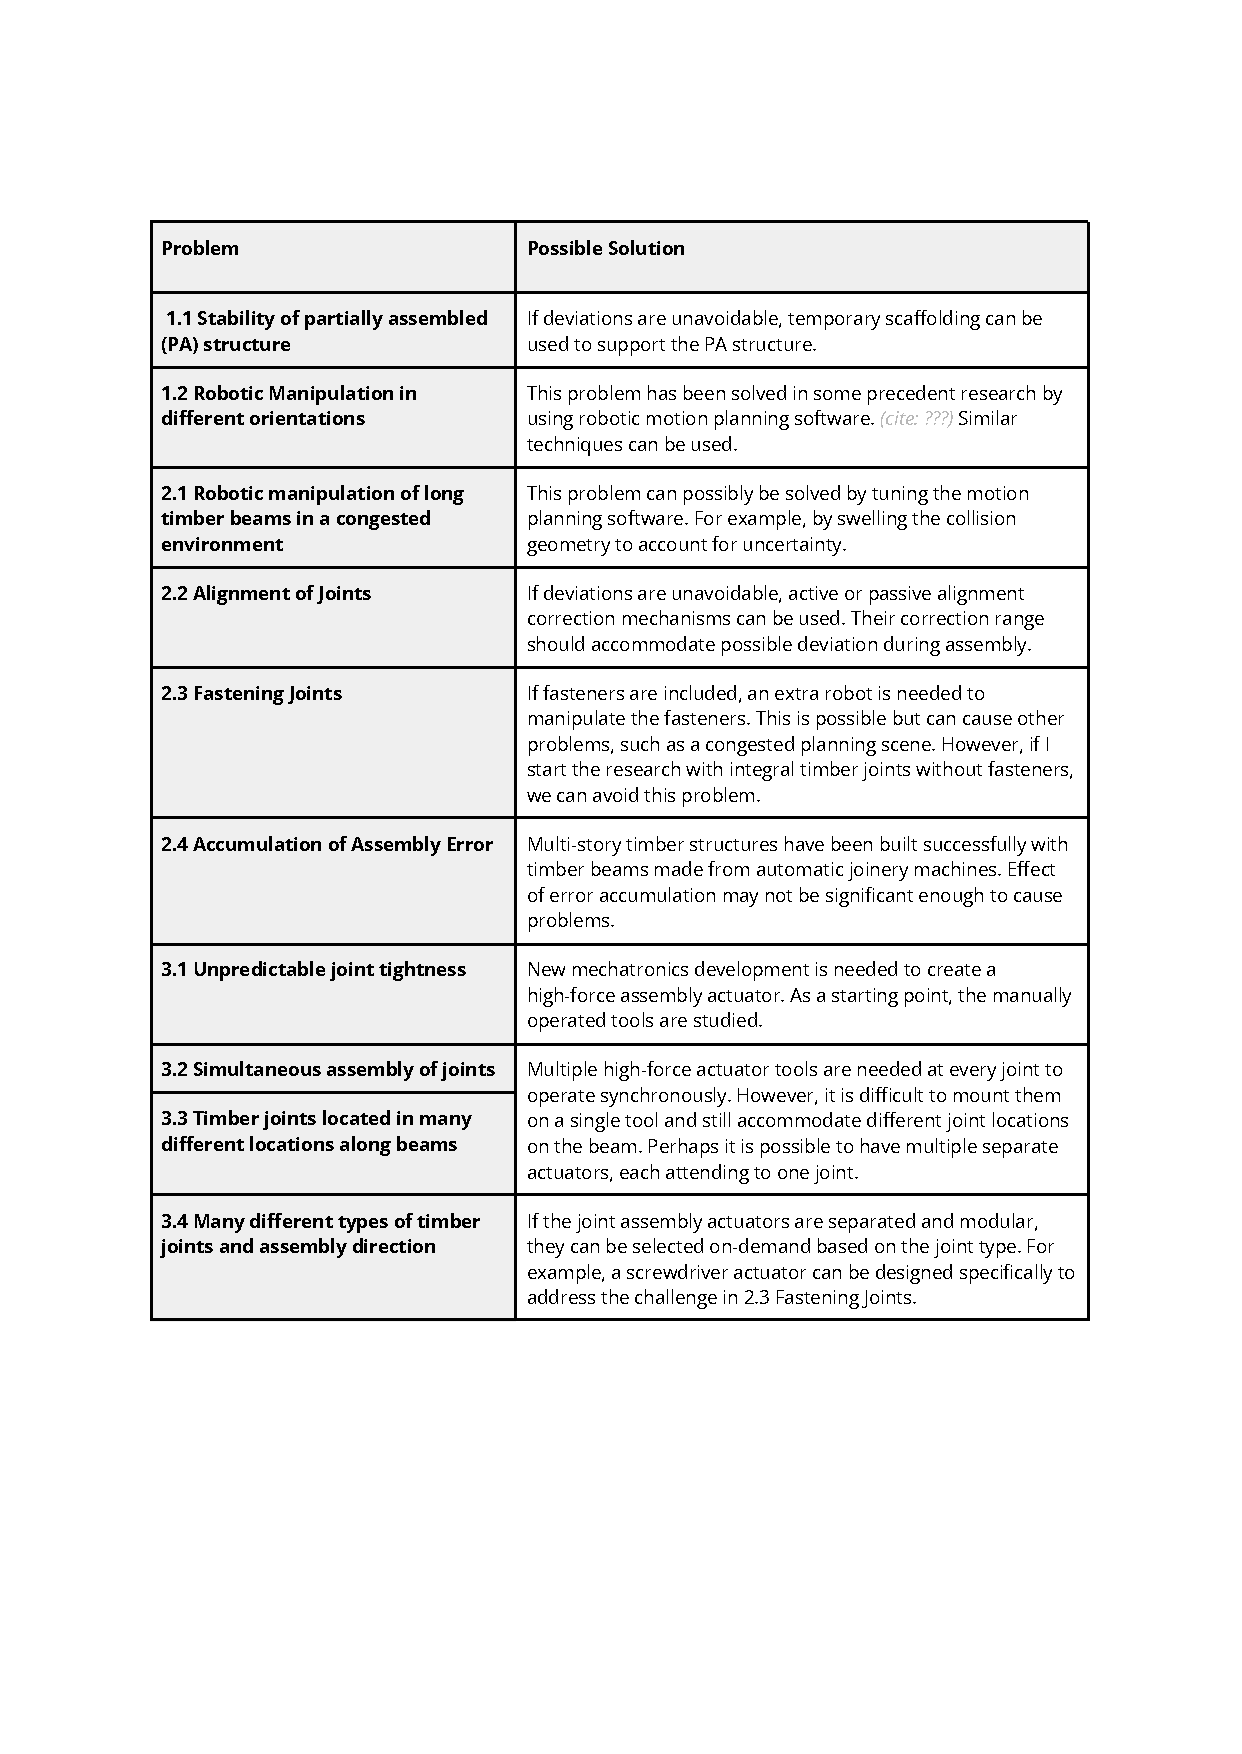
\includegraphics[page=1, trim=25.4mm 60mm 25.4mm 33mm, clip, width=\textwidth]{tables/Tables in Chapter 4.pdf}
    \caption{Author's response to the assembly challenges}
    \label{table:response-to-challenges}
\end{table}

I conducted a survey of tools used by carpenters to applying assembly force for closing joints. The first is a hammer-type tool.\footnote{There are other names for the carpentry hammer, such as mallet, beetle} The striking action of a hammer delivers a short but strong spike of force that momentarily overcome friction to drive joints together. However, it is only effective if a striking surface is available near the joint, as the flexible timber material can absorb the shock. Moreover, hammers are ineffective if the striking direction is upright, as it is difficult to work against gravity. 

The second is a joint-puller-type tool. It often consists of a pair of hooks that can be tightened by a screw or ratcheting mechanism. The hooks can be hammered into the timber or hooked into pre-drilled holes on both sides and pull the joint together. Joint-pullers are particularly useful for pulling liner elements along its length, such as in a splice joint, where a striking surface is not available near the joint. 

The third is a clamp-type tool. It is often used for lap joints where parallel surfaces are easily reachable for clamping. Among different designs, F-shaped clamps are often used because their opening can be quickly adjusted. The joint puller type and the clamp type tools can be used in various orientations regardless of the direction of gravity and they can also be used as a means of temporary support after they are tightened. 

For beams that require the assembly of multiple joints, it is common for multiple workers to actuate the assembly tools synchronously. Because the assembly tools can only apply local forces to each pair of joints, if the assembly motion is not synchronised, the overall beam will deviate from the assembly trajectory (e.g. starts to rotate) and can get stuck due to the jamming effect. This problem is similar to the peg-hole insertion jamming problem studied in robotic assembly. \parencite{dupontJammingWedgingConstrained1994} Therefore, assembly workers need to keep an eye on the overall progress of the entire beam and adjust their actuation speed or hammering force accordingly. 

\subsection{Distributed Robotic Tool (DiRT) Approach}
\label{subsection:exploration-1-distributed-robotic-tool-approach}

From the insights gained from challenges 3.2 to 3.4, it became evident that deploying multiple high-force assembly actuators on each mating joint is a promising approach. Moreover, these actuators should not be fixed together such that it is flexible to position them where the joints are. However, it is challenging to use one robotic arm to hold each end-effector during operation as the number of robots needed may result in congestion near the active beam. Furthermore, this approach is not scalable when working with timber elements that have a large number of joints. 

Therefore, I hypothesised a scenario in which the actuators are attached to and hanging from the Partially Assembled (PA) structure. The attachment and detachment of the tools can therefore be performed one by one, using as few as one robotic arm. After all the actuators are in place, the robotic arm can bring the next piece of timber towards the joints, and perform the assembly with all the actuators exerting force locally at each joint. Because these actuators are no longer tethered to the rest of the robotic system, I called this a “Distributed Robotic Tool” (DiRT) approach. 
This distributed approach does not only address the robot congestion issue but also enhances the scalability and flexibility of the system, making it better suited for timber assembly tasks with varying levels of complexity. The modularity of distributed tools allows for the development of different tools tailored to different joint types and assembly requirements. The system can intelligently select the appropriate tool based on the design of a structure, joint types, and joint angles. This adaptability ensures that the DiRT approach can effectively address a wide range of timber frame structures.

\subsection{Scope for Initial Exploration Round}
\label{subsection:exploration-1-scope-for-initial-exploration-round}

Because the design of a DiRT assembly tool is specific to the joint type, I had to make a decision on which joint type to be developed first. Among the popular types of timber joints used in timber frame structures, I decided to start the investigation with lap joints. This is because lap joints are the most versatile type of joints that can be used to join many structural members. For details, please see \noseeref{subsection:exploration-1-lap-joint-classification-by-assembly-direction} regarding the definition of Lap Joints used in this thesis and their versatility.

\begin{figure}
    \centering
    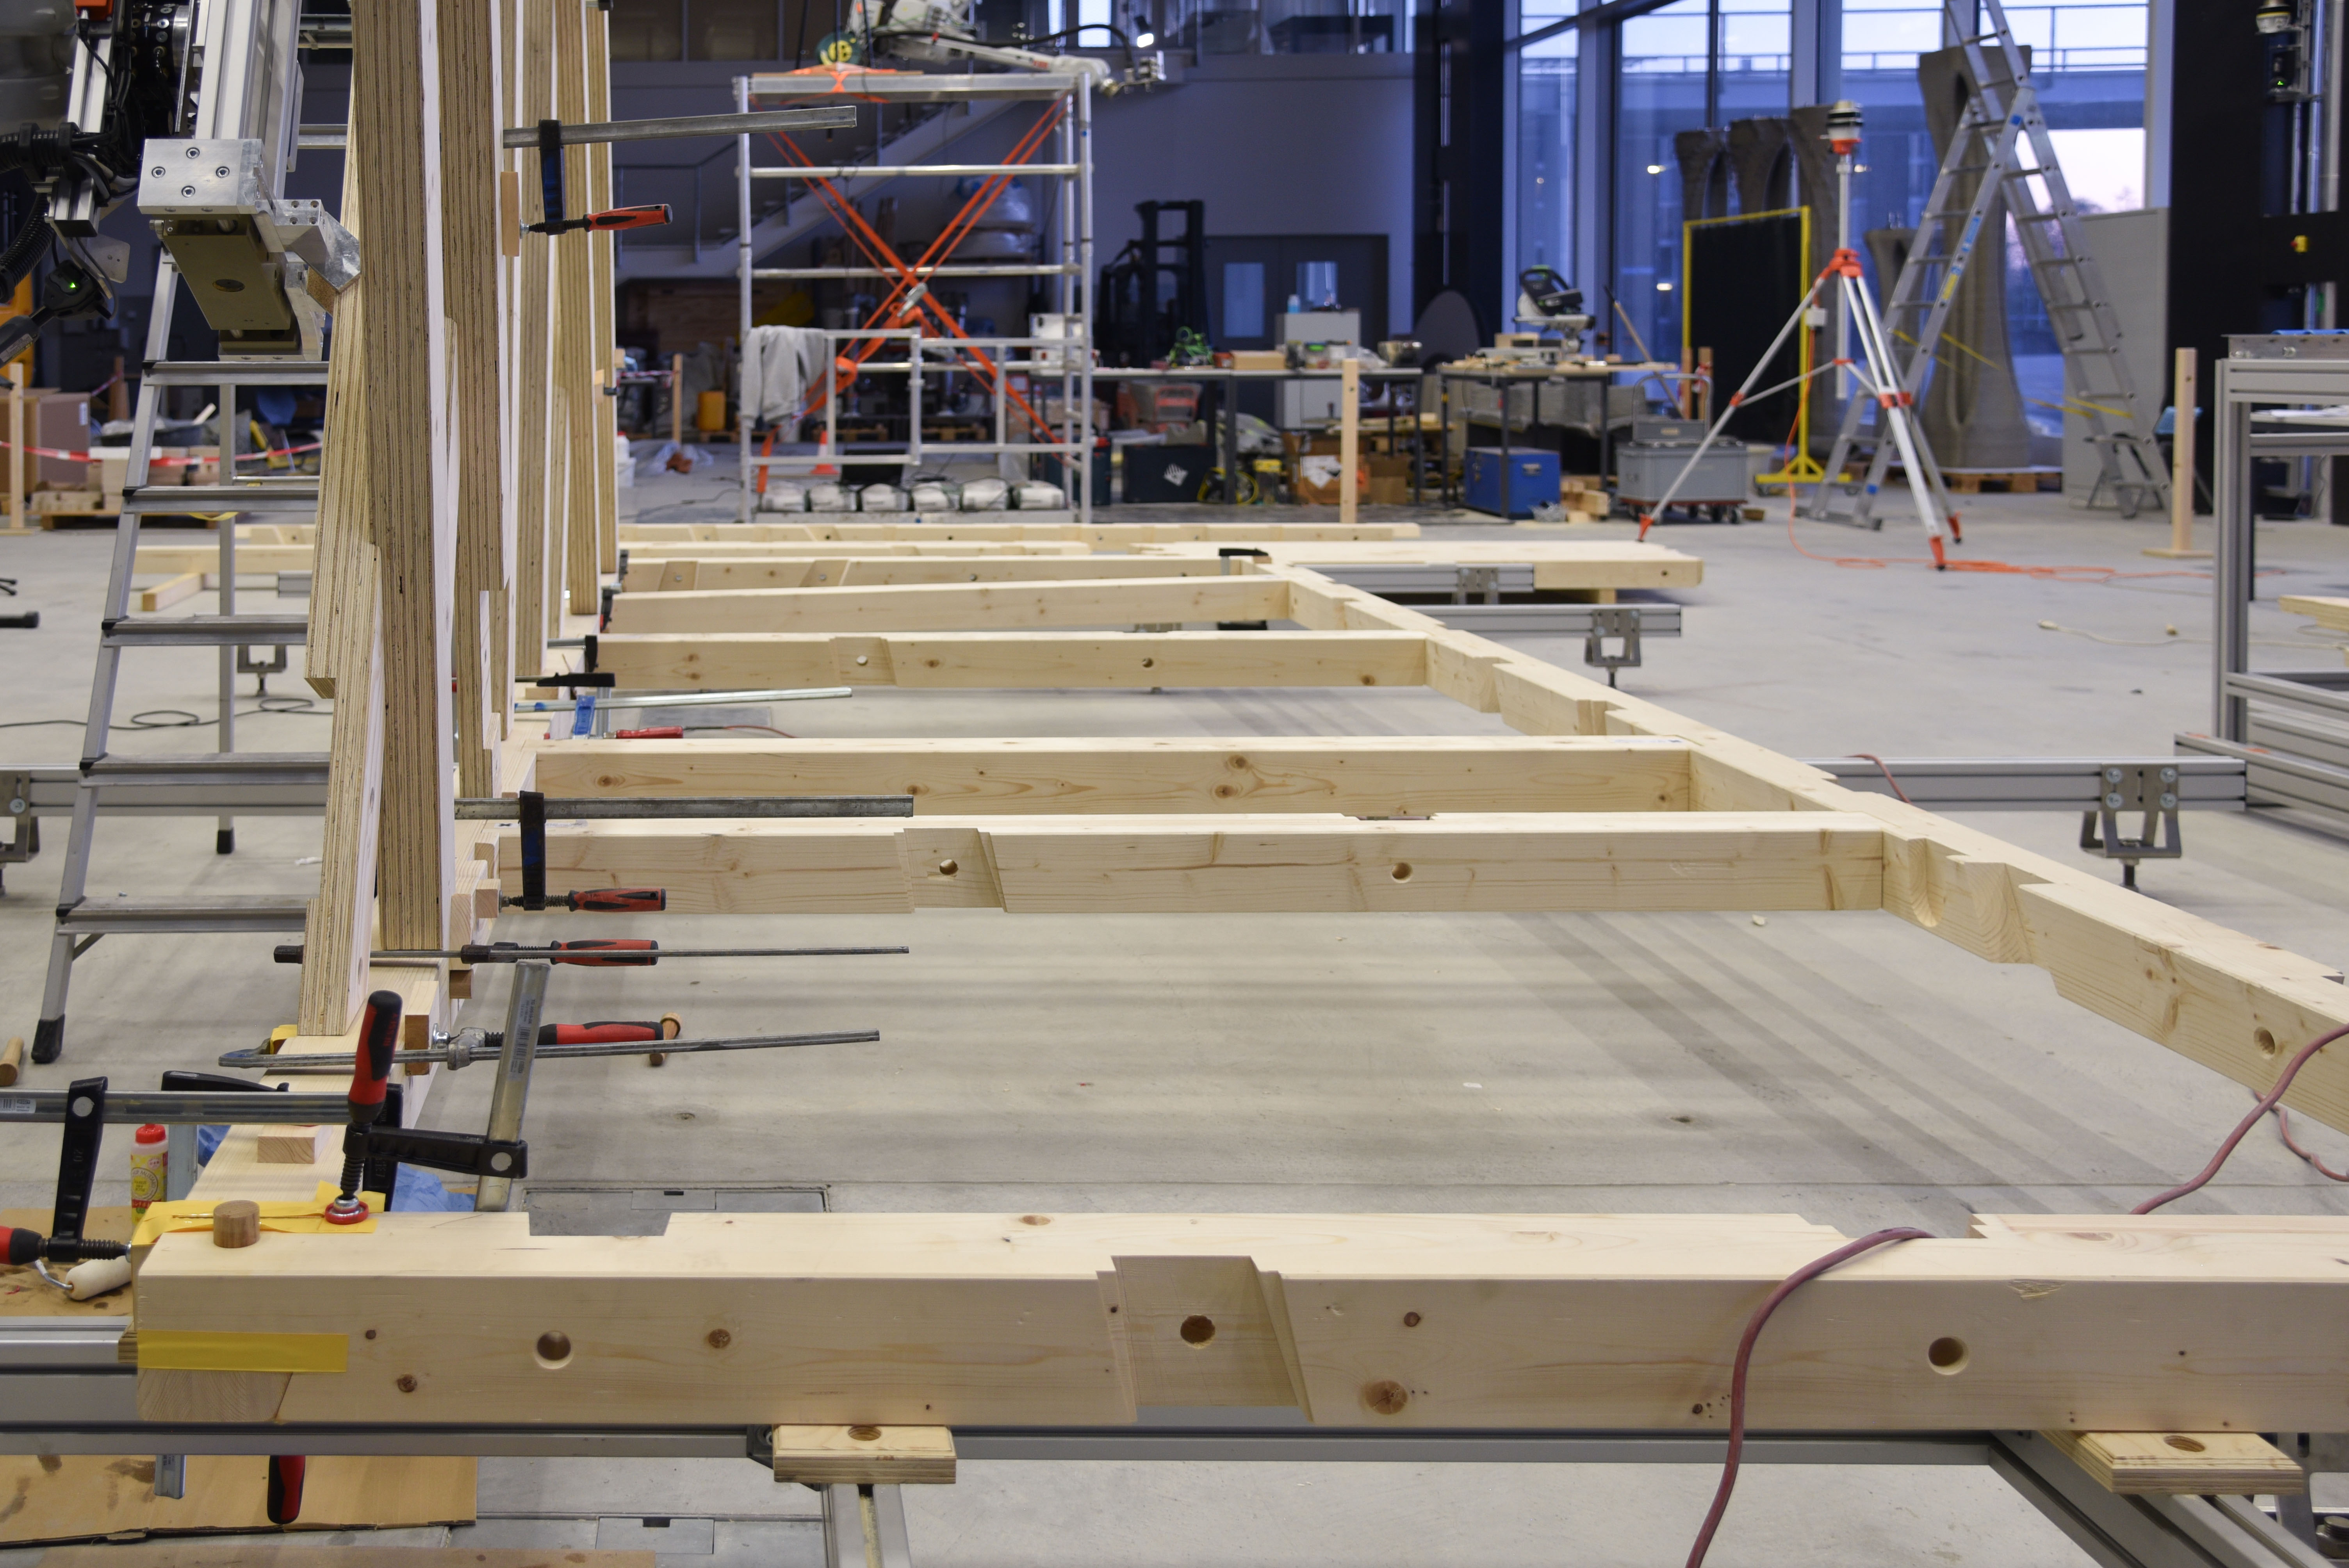
\includegraphics[width=0.99\textwidth]{images/04-1+2/clamp-inspiration.jpeg}
    \caption{Example of carpentry clamps used in timber construction.}
    \label{fig:clamp-inspiration}
\end{figure}

Based on a review of the manual tools used for assembling lap joints, I have shortlisted two promising actuator arrangements. The first arrangement is a clamping mechanism similar to carpentry clamps, which apply a compression force to the outside of the lap joints (see Figure \ref{fig:clamp-inspiration}). The second arrangement is a screwing mechanism that uses a screw to pull the two sides of a joint together. I decided to start the development with the clamping mechanism because it is mechanically simpler. In later exploration rounds, the screwing mechanism was also explored \seeref{section:exploration-4-goal}.

In this exploration round, the focus is to:
\begin{itemize}
    \item Validate the robotic clamping streategy for the assembly of lap joints, starting with an orthogonal lap joint.
    \item Explore streategies for hanging a robotic clamping tool on the timber structure.
\end{itemize}

This is achieved through a series of mechatronics development to create a robotic clamp. On the other hand, other essential features of DiRT operations such as remote control, battery packs and wireless communication systems are postponed to later development.
In order to simplify initial development, I decided to pick a timber size standard of \textbf{100x100mm square profile}. This is selected after careful consideration to fulfil the following criteria:
\begin{itemize}[nosep]
    \item A profile size commonly available in Switzerland to facilitate demonstrations and experiments.
    \item A profile big enough to be strong structurally and can be used as beams, columns and bracings.
    \item A profile small enough such that the robotic arm in the lab (with its limited payload) can manipulate a long beam.
\end{itemize}

For the timber species and processing, I chose \textbf{glue-laminated spruce} as the intended material because it is one of the most commonly used construction timber in Switzerland. The timber material used in this thesis has the following properties:

\begin{itemize}[nosep]
    \item Strength class: GL24h 
    \item Appearance class: N
    \item Lamination composition: Duo or Trio
    \item Gluing standard: DIN EN 14 080 
    \item Moisture Content 13\% ± 3\%
    \item Nominal Density 460kg/m3
\end{itemize}

\subsection{DiRT Clamping Assembly Process Task List (Version 1)}
\label{subsection:exploration-1-dirt-clamping-assembly-process-task-list-v1}

The working hypothesis of the Distributed Robotic Tool (DiRT) System for timber frame assembly consists of two main hardware components:
\begin{itemize}[nosep]
    \item A set of distributed robotic clamps (the “clamps”), each of which $\cdots$
    \begin{itemize}
        \item Can be attached to the joint area
        \item Can perform a clamping action on lap joints
        \item Can be operated wirelessly and synchronously
    \end{itemize}
    \item A robotic arm mounted on gantry axes (the “robot”) that $\cdots$
    \begin{itemize}
        \item Can attach clamps on the Partially Assembled (PA) structure
        \item Can bring a timber beam to the clamps
        \item Can move the timber beam together while the clamps are clamping
        \item Can retrieve the clamps after they are finished
    \end{itemize}
\end{itemize}

Their operation is based on a repetitive cycle for every beam to be assembled. Table \ref{table:list-of-assembly-tasks} describes a list of tasks according to their order of operation and a shortened name for referring to them later in this thesis.

\begin{table}[H]
    \includegraphics[page=2, trim=25.4mm 100mm 25.4mm 33mm, clip, width=\textwidth]{tables/Tables in Chapter 4.pdf}
    \caption{List of tasks in a repetitive cycle for assembling timber beams}
    \label{table:list-of-assembly-tasks}
\end{table}

% \clearpage

\begin{figure}[p]
    \centering
    \begin{subfigure}[b]{0.49\textwidth}
        \centering
        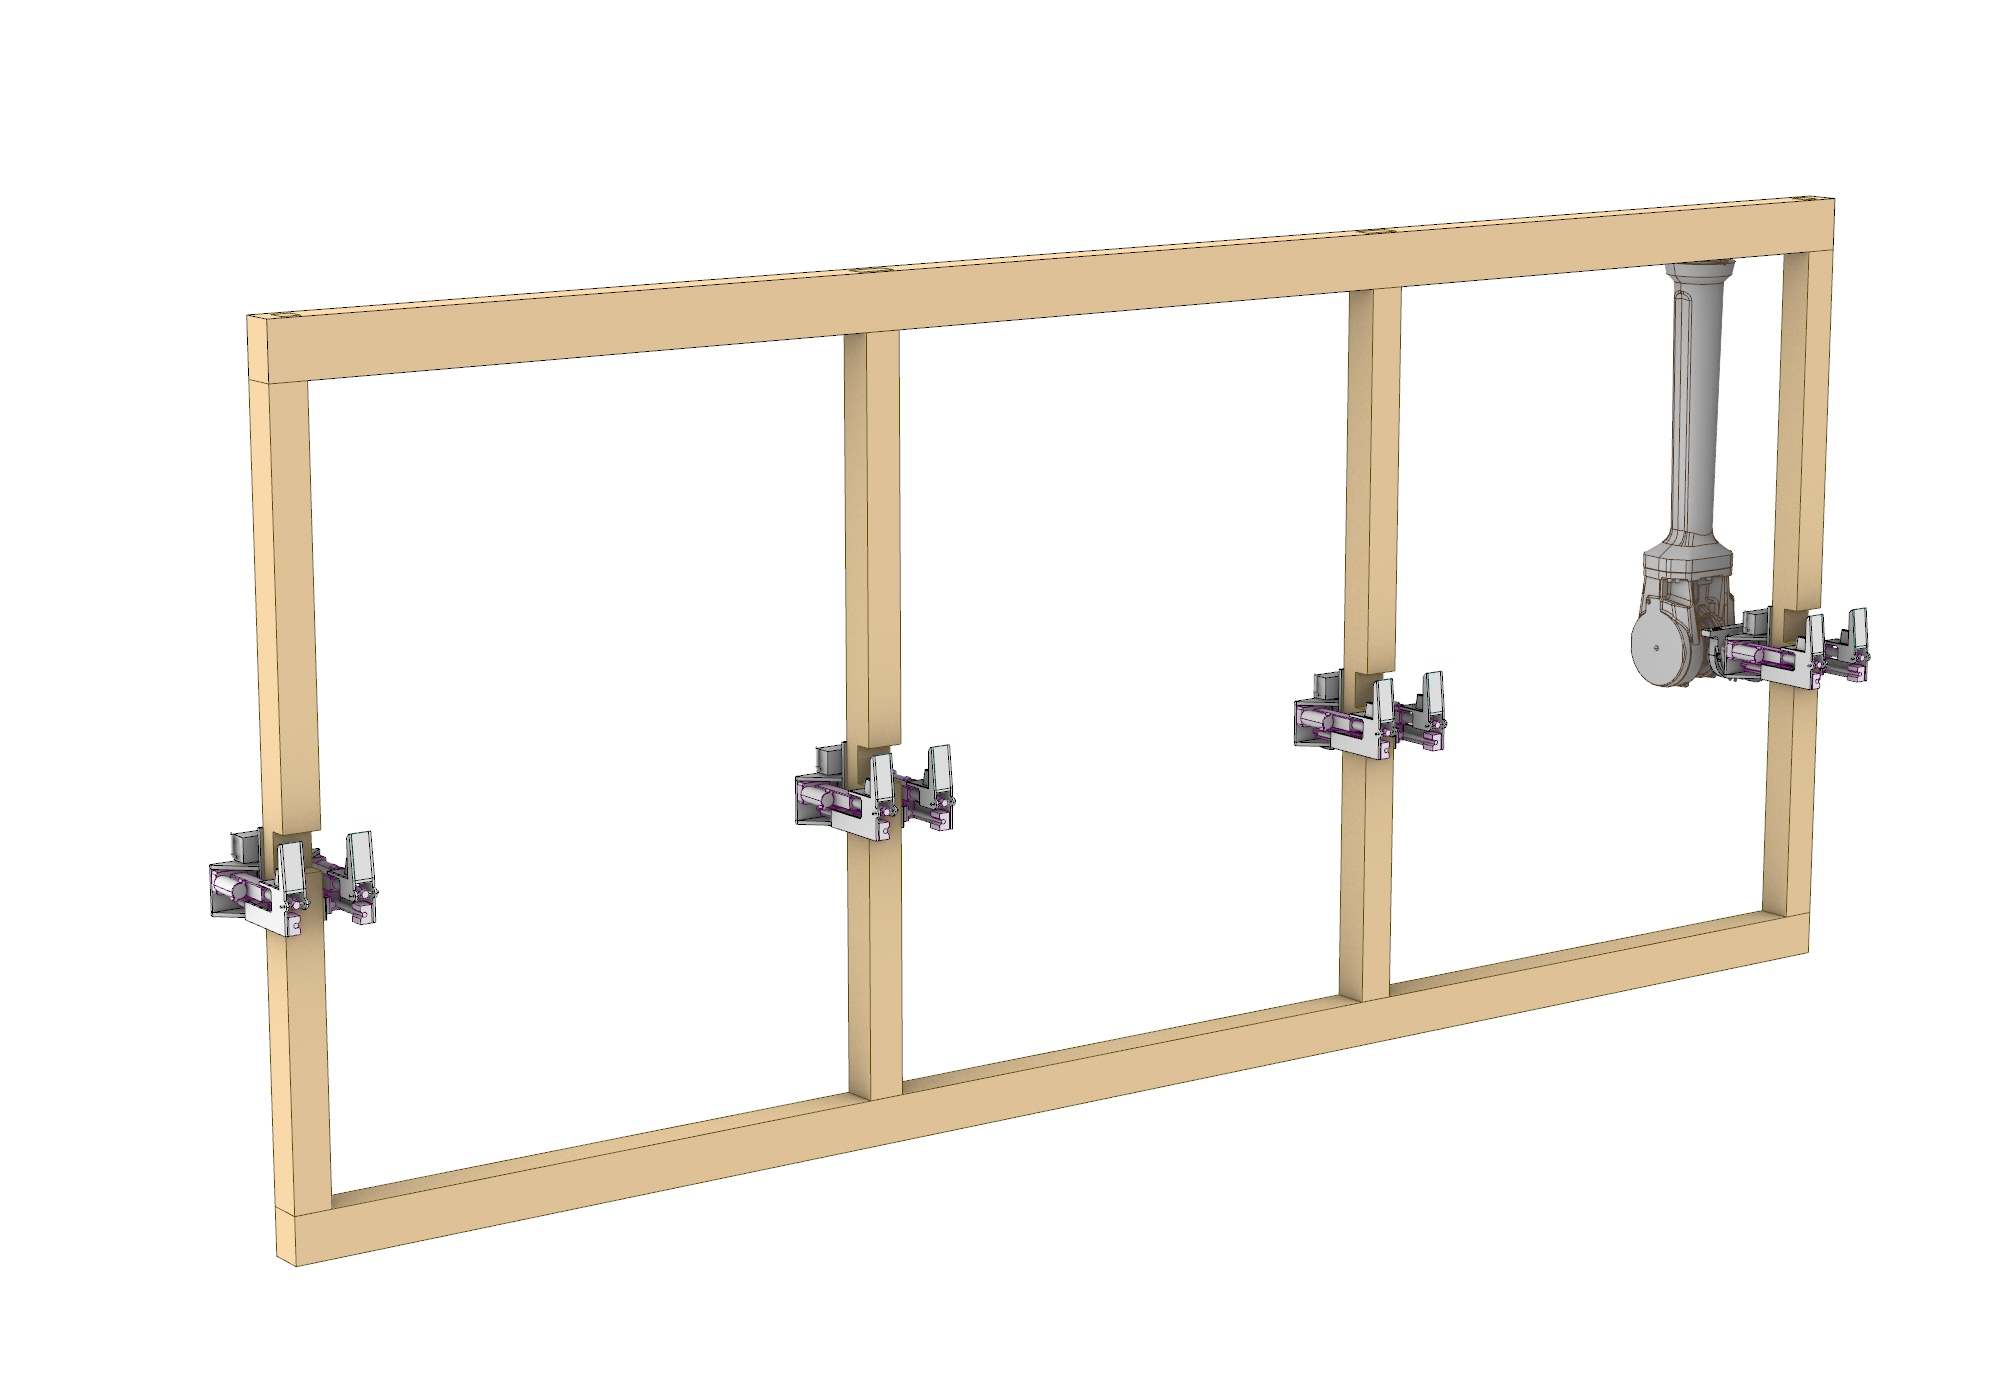
\includegraphics[width=\textwidth]{images/04-1+2/Multiple_4.jpg}
        \caption{The moment after the fourth {\tt PlaceClampToStructure}}
        \label{fig:fig:beam-assembly-step1}
    \end{subfigure}
    \hfill
    \begin{subfigure}[b]{0.49\textwidth}
        \centering
        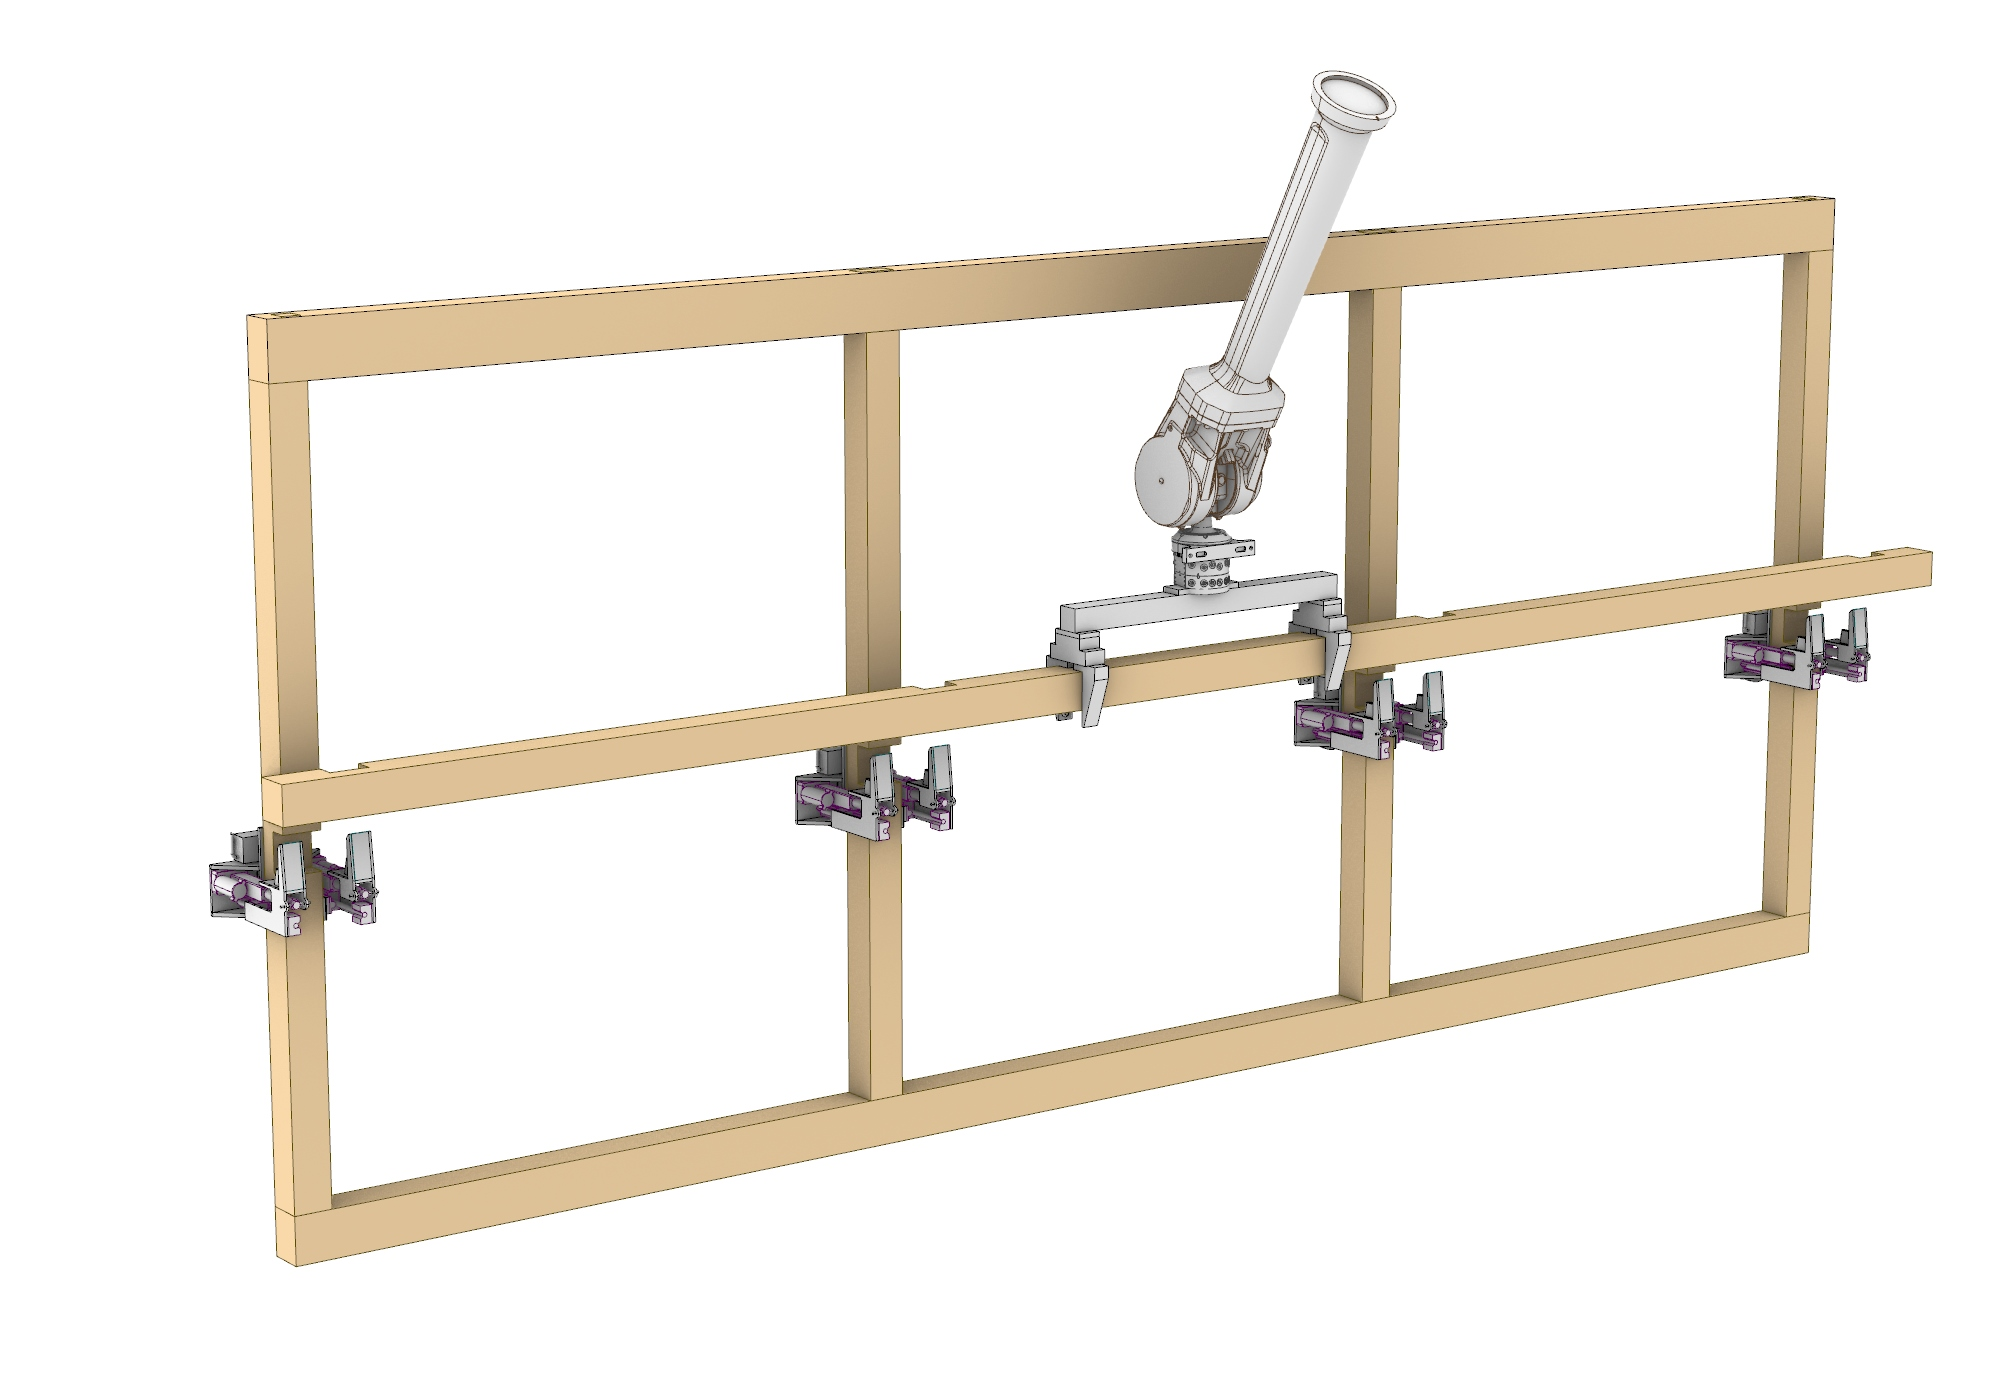
\includegraphics[width=\textwidth]{images/04-1+2/Multiple_5.jpg}
        \caption{The moment after \codett{BeamTransfer} but before \codett{ PlaceBeamInClamp}}
        \label{fig:fig:beam-assembly-step2}
    \end{subfigure}
    \vskip\baselineskip % Next row
    \begin{subfigure}[b]{0.49\textwidth}
        \centering
        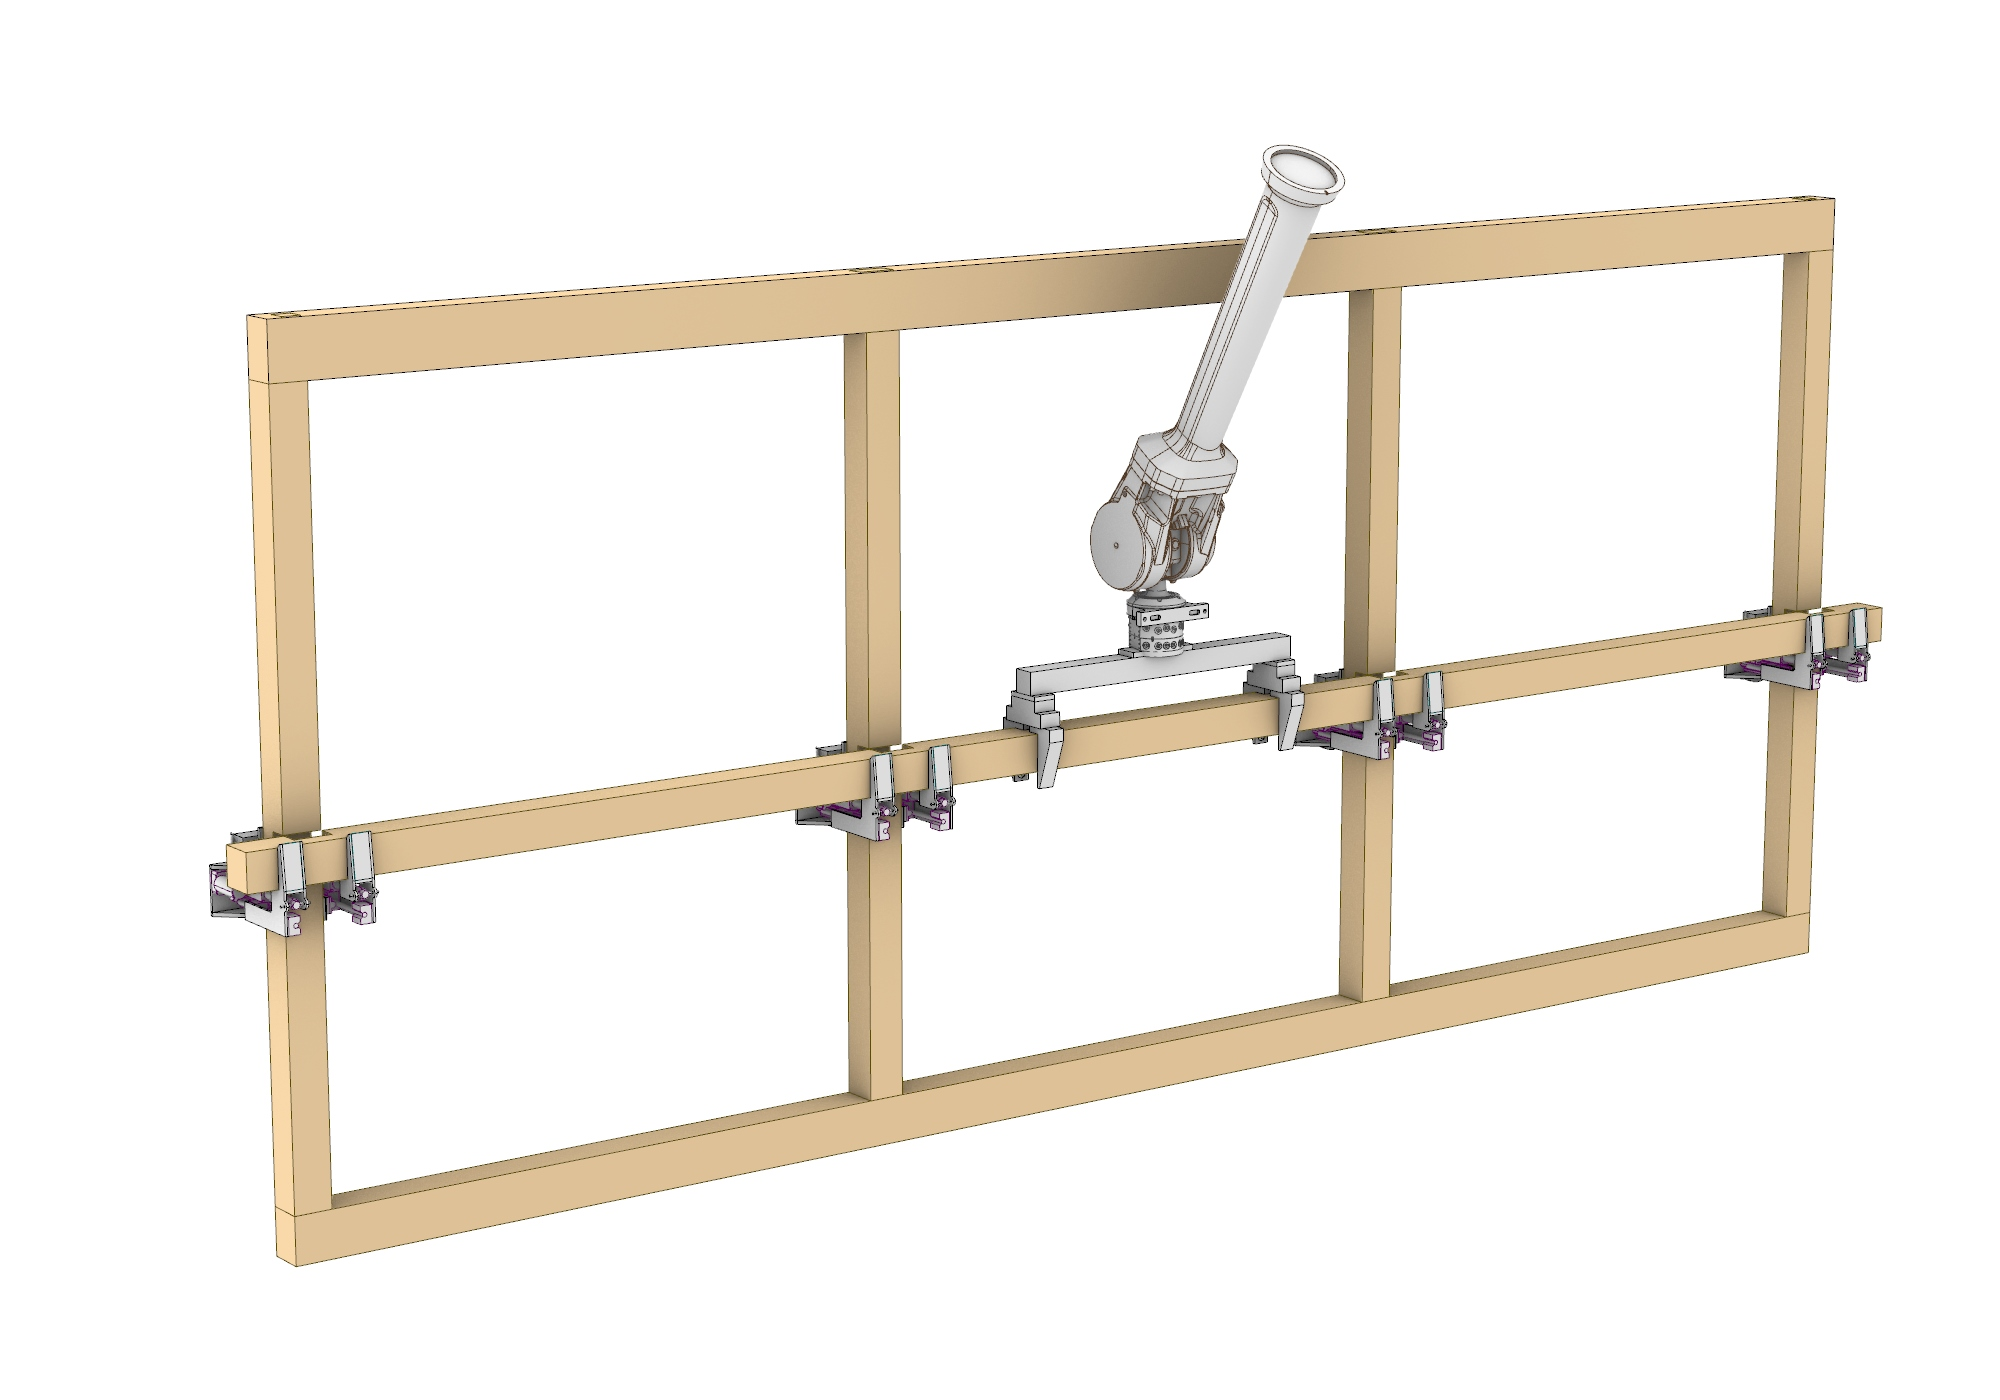
\includegraphics[width=\textwidth]{images/04-1+2/Multiple_7.jpg}
        \caption{The moment after {\tt PlaceBeamInClamp}}
        \label{fig:fig:beam-assembly-step3}
    \end{subfigure}
    \hfill
    \begin{subfigure}[b]{0.49\textwidth}
        \centering
        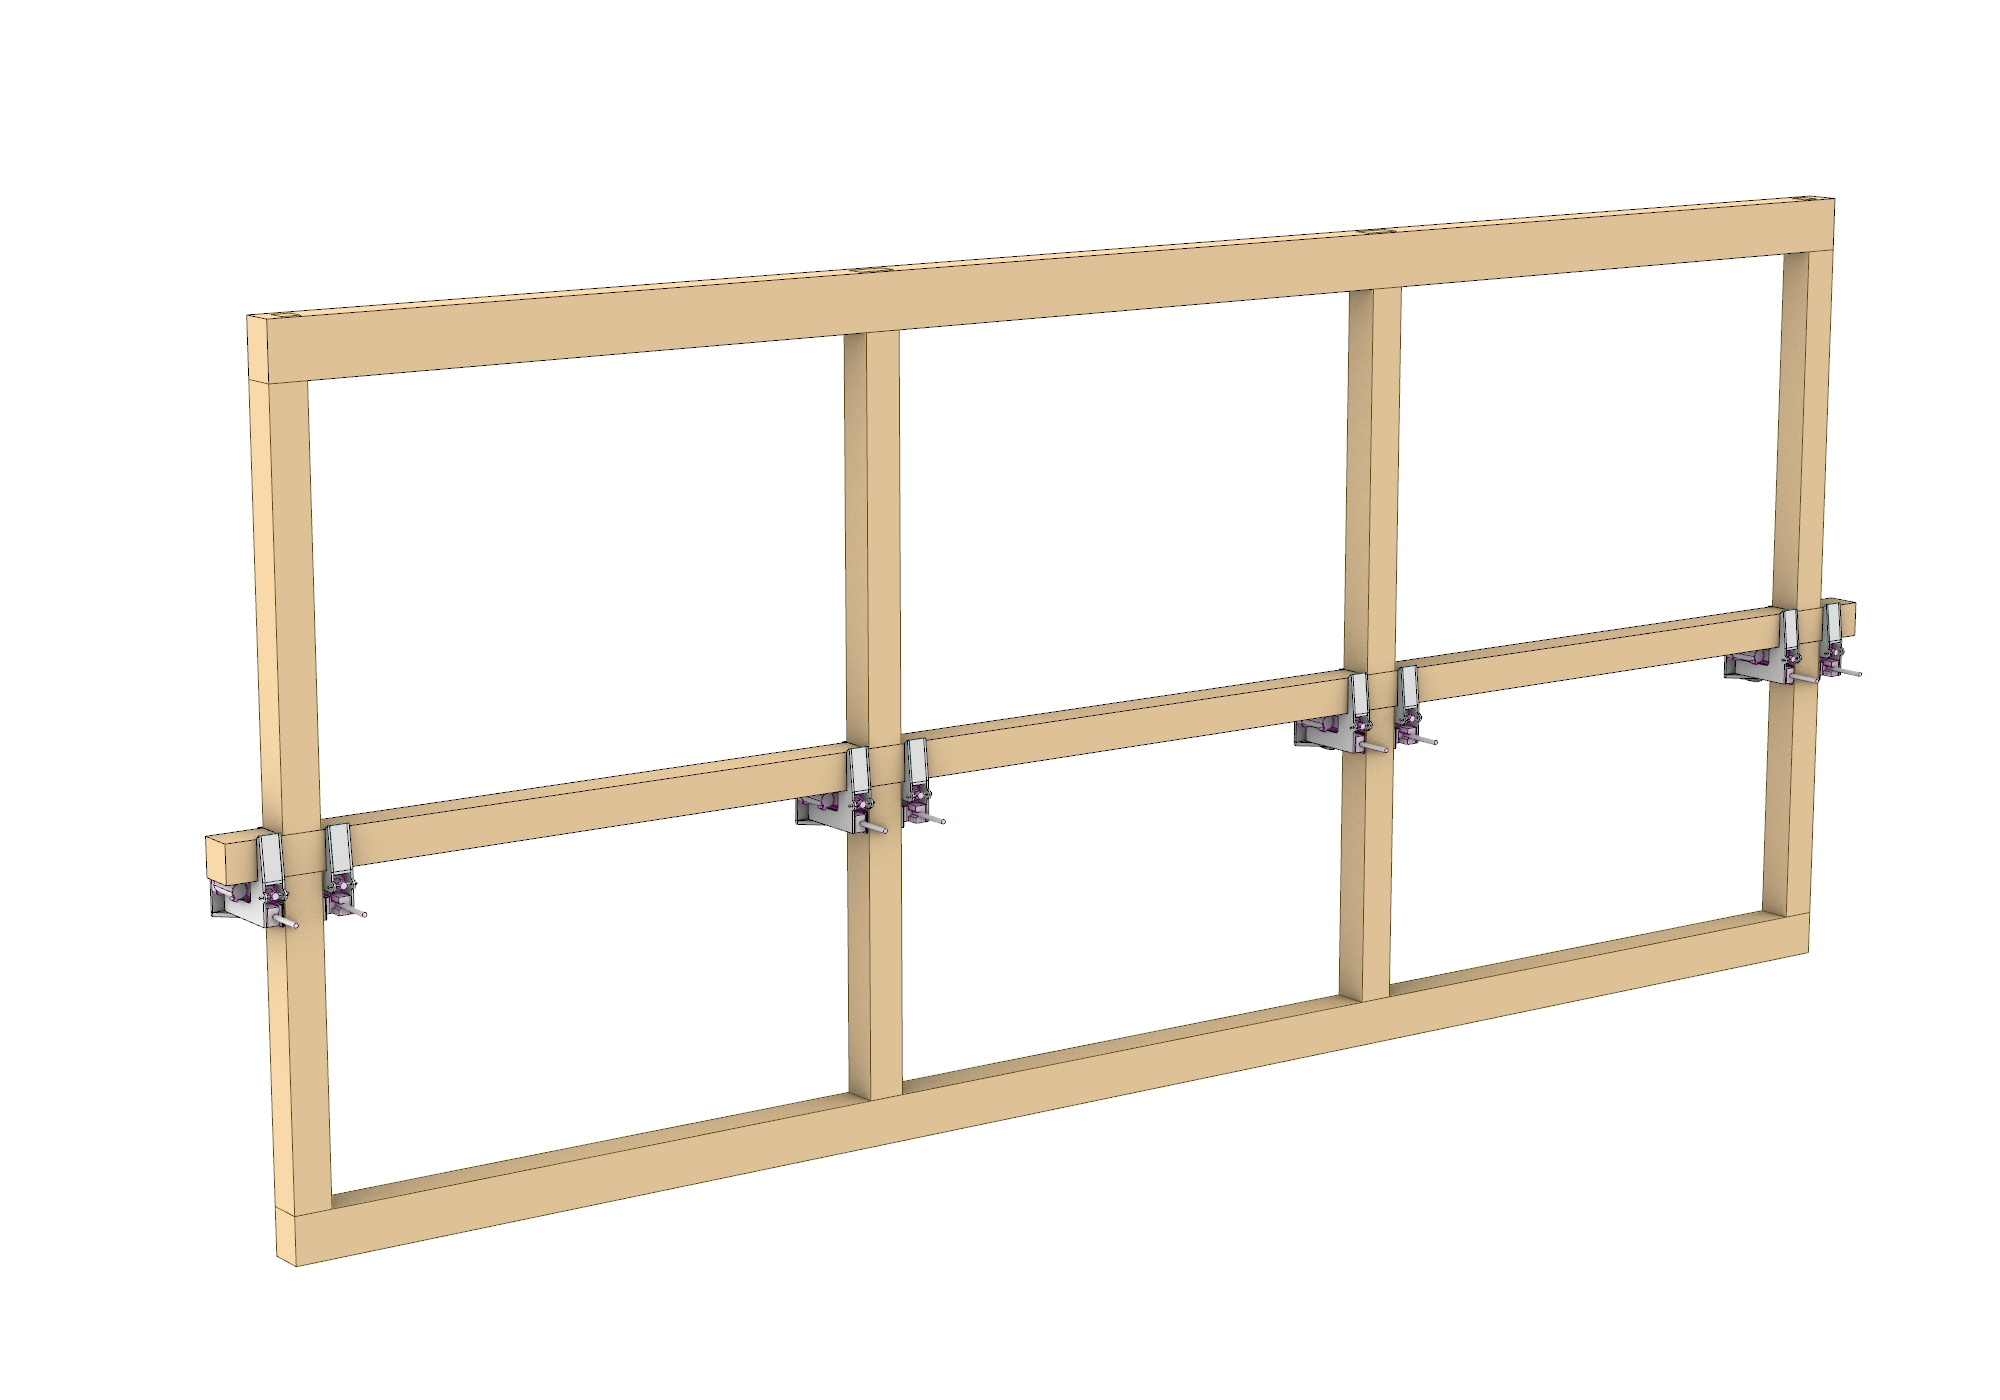
\includegraphics[width=\textwidth]{images/04-1+2/Multiple_10.jpg}
        \caption{The moment after {\tt ClampSyncAssembly}}
        \label{fig:fig:beam-assembly-step4}
    \end{subfigure}
        \vskip\baselineskip % Next row
    \begin{subfigure}[b]{0.49\textwidth}
        \centering
        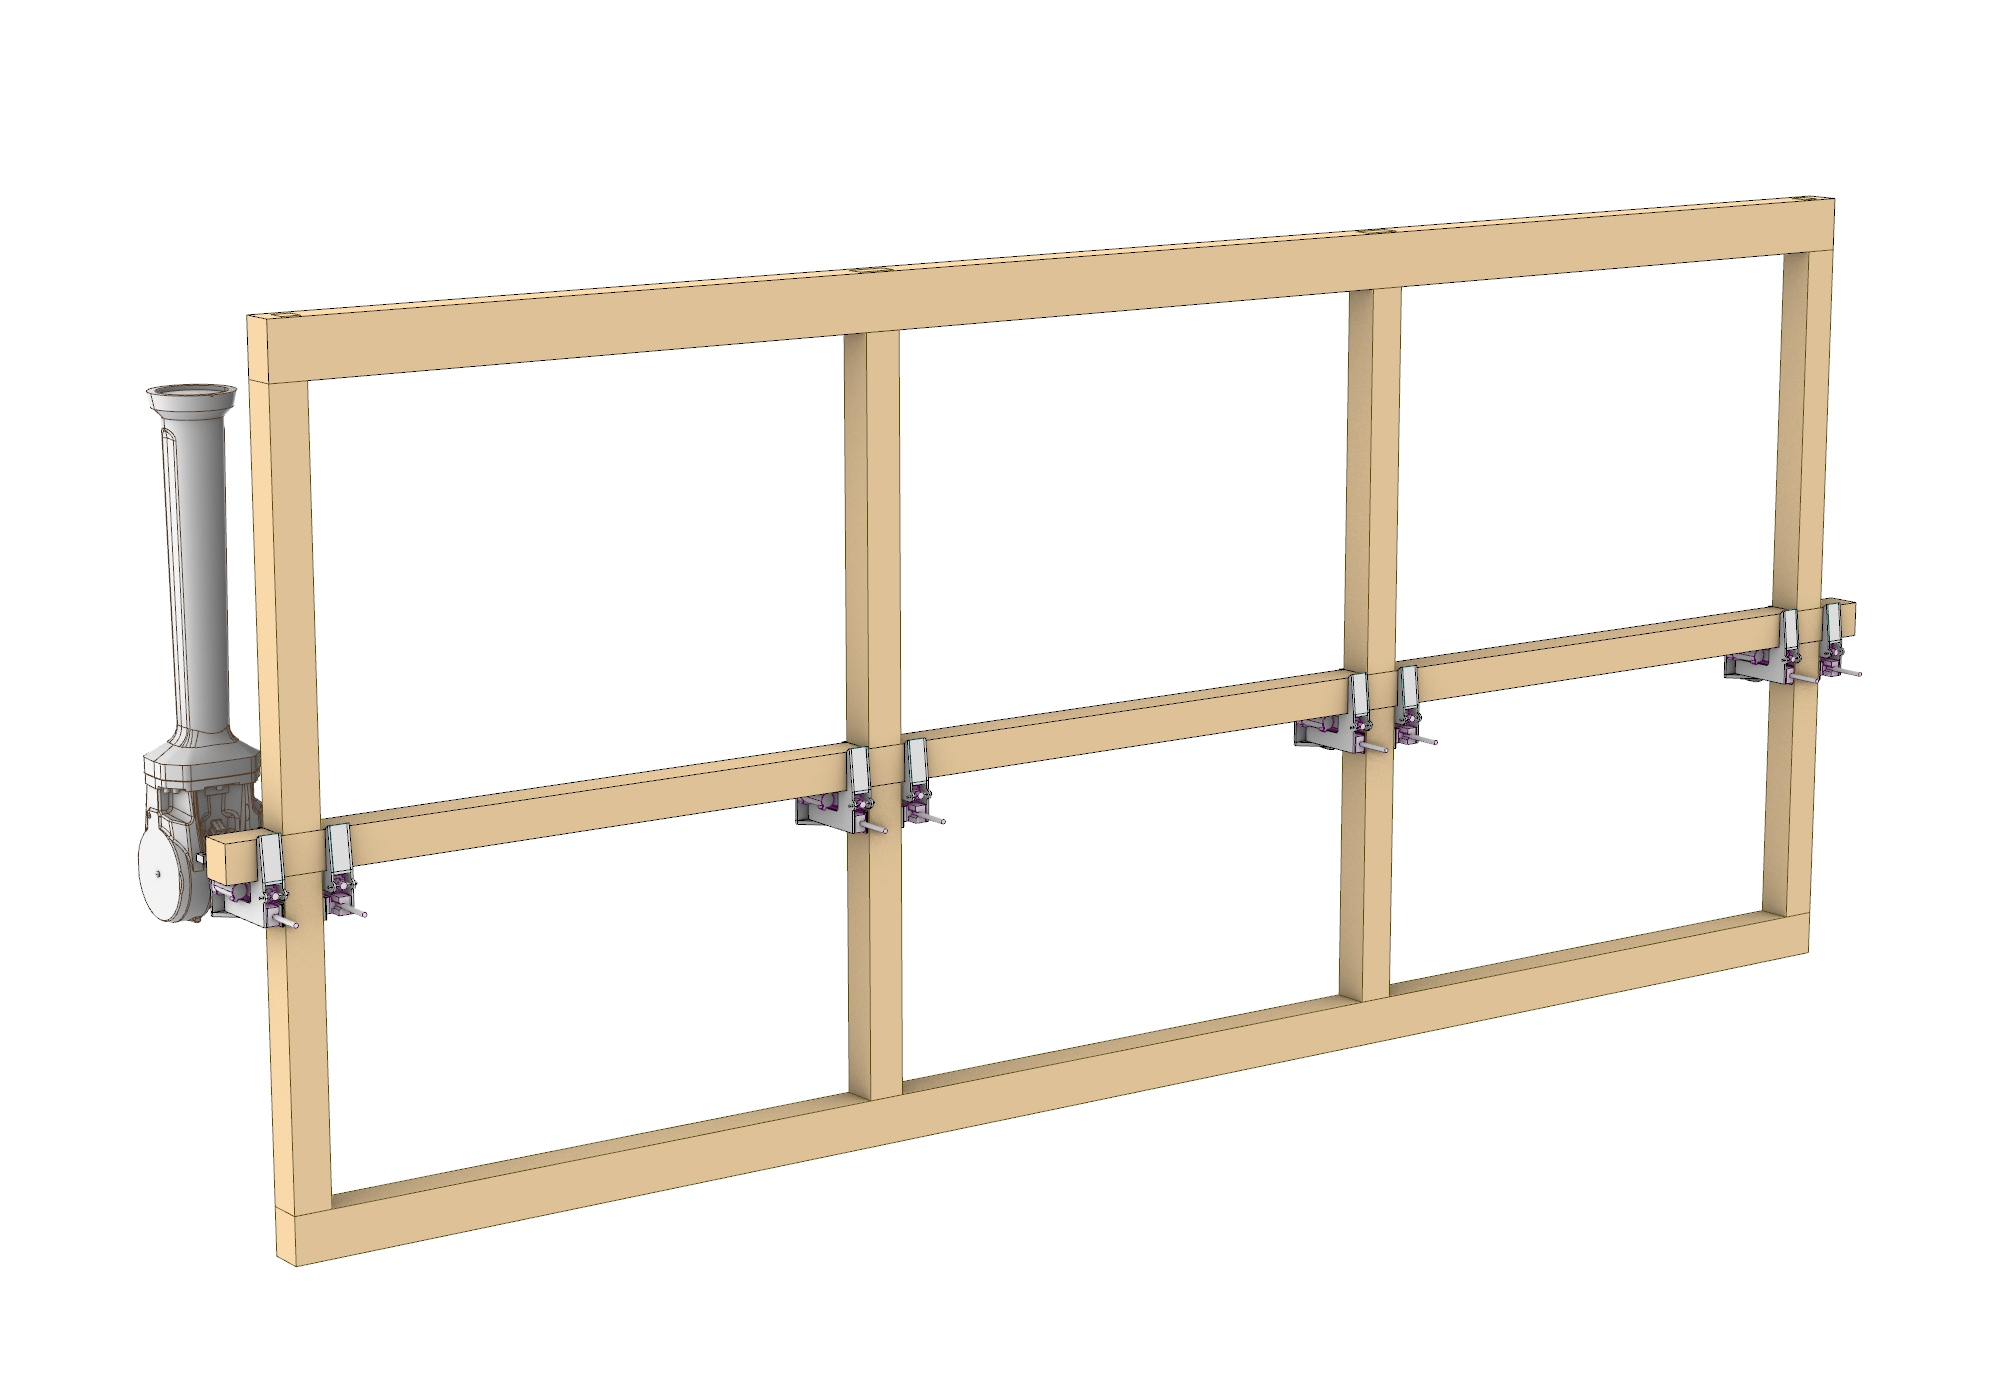
\includegraphics[width=\textwidth]{images/04-1+2/Multiple_11.jpg}
        \caption{The moment before the first {\tt PickClampFromStructure}}
        \label{fig:fig:beam-assembly-step5}
    \end{subfigure}
    \hfill
    \begin{subfigure}[b]{0.49\textwidth}
        \centering
        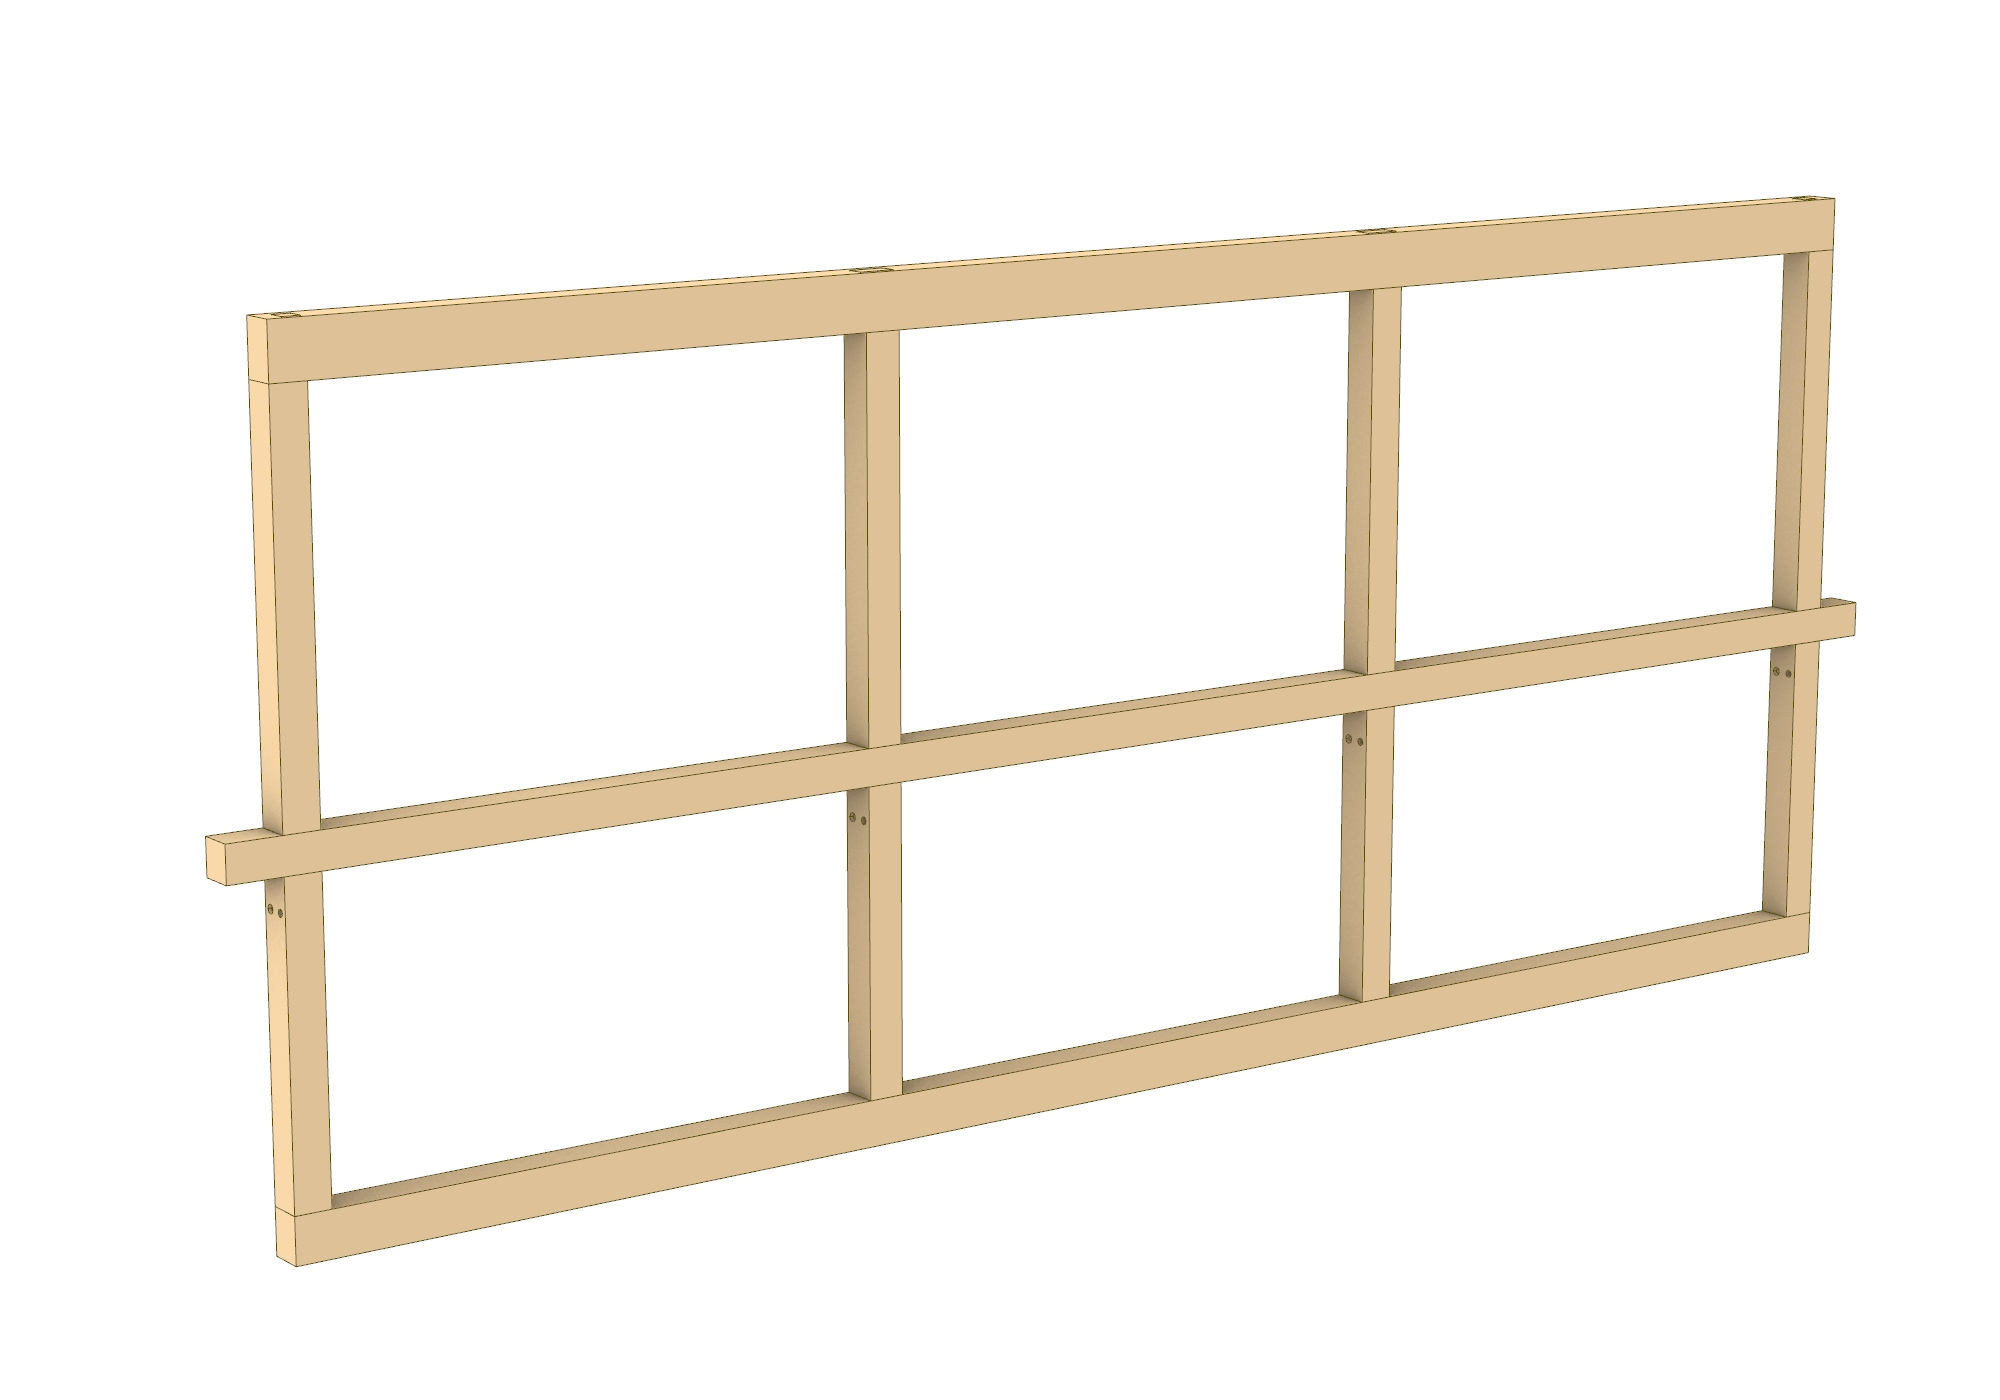
\includegraphics[width=\textwidth]{images/04-1+2/Multiple_15.jpg}
        \caption{The moment at the end of the cycle, after the last {\tt PlaceClampToStorage}}
        \label{fig:fig:beam-assembly-step6}
    \end{subfigure}
    \caption[Diagrams illustrating the assembly steps of a horizontal beam]
    {Diagrams illustrating the assembly steps of a horizontal beam (refer to Table \ref{table:list-of-assembly-tasks} for the description of each step)}
    \label{fig:beam-assembly-six-moments}
\end{figure}

\FloatBarrier

Figure \ref{fig:beam-assembly-six-moments} illustrates the assembly process of a horizontal beam with four simultaneous mating joints. In this initial working hypothesis, the system requires manually assembling the first few columns to the ground before the subsequent process can become fully automatic. At this point, I have not considered how to assemble non-vertical elements. However, this became clear at the end of this exploration round \seeref{subsection:exploration-1-beam-support-needed-during-clamping}.

% \clearpage

\section{Background}
\label{section:exploration-1-background}

\subsection{Lap Joint Classification by Assembly Direction}
\label{subsection:exploration-1-lap-joint-classification-by-assembly-direction}

Timber frame buildings utilize a variety of joints to connect structural elements and create a stable, load-bearing framework. Various categorisation methods have been developed to group them based on their characteristics, functions, or cultural background \seeref{subsection:introduction-defining-characteristics}. As the primary objective of this thesis is to investigate the assembly process of timber frame structures, I adopted a classification method that focuses on the assembly direction of the joints, because it is closely related to the kinematics of the assembly tools.

Lap joints, mortise and tenon joints, and splice joints are three common types of joints found in timber frame construction, each with different assembly directions in relation to the neighbouring elements' arrangements. This thesis focus on the assembly of lap joints, as they represent a straightforward and widely used connection method in timber frame construction. 

Lap joints are formed by overlapping two pieces of timber, with one piece lying on top of the other. The overlapping sections are typically cut to half the thickness of the timber, creating a flush surface.\footnote{Note that in some classifications \parencite{seikeArtJapaneseJoinery1977}, lap joints are not necessarily planar or assembled perpendicular to the flush face. However, this narrower definition simplified the initial development.} Lap joints are widely used in timber frame construction due to their versatility and ability to transfer loads between connected elements effectively. These joints are relatively simple to assemble, as they involve linear assembly motion that is perpendicular to the flush surface. 

Figure \ref{fig:common-joints-crosslap} and \ref{fig:common-joints-teelap} shows cross-shape and tee-shape lap joint, both conform to the lap joint definition used in this thesis. Figure \ref{fig:common-joints-mortisetenon} shows a counter-example, a mortise and tenon joint, where the assembly direction is parallel to one of the element’s axes. Later in Exploration Round 2, the definition of lap joints was expanded to include joints that have parametric angle variation \seerefii{subsection:exploration-2-parametric-variations-of-lap-joints}{subsection:exploration-4-parametric-polyline-lap-joints}. In Exploration Round 5, it is further expanded to compound angles out-of-plane \seeref{subsection:exploration-4-parametric-non-planar-lap-joints}. 

% 3 Horizontal Image  
\begin{figure}[H]
     \centering
     \begin{subfigure}[b]{0.32\textwidth}
         \centering
         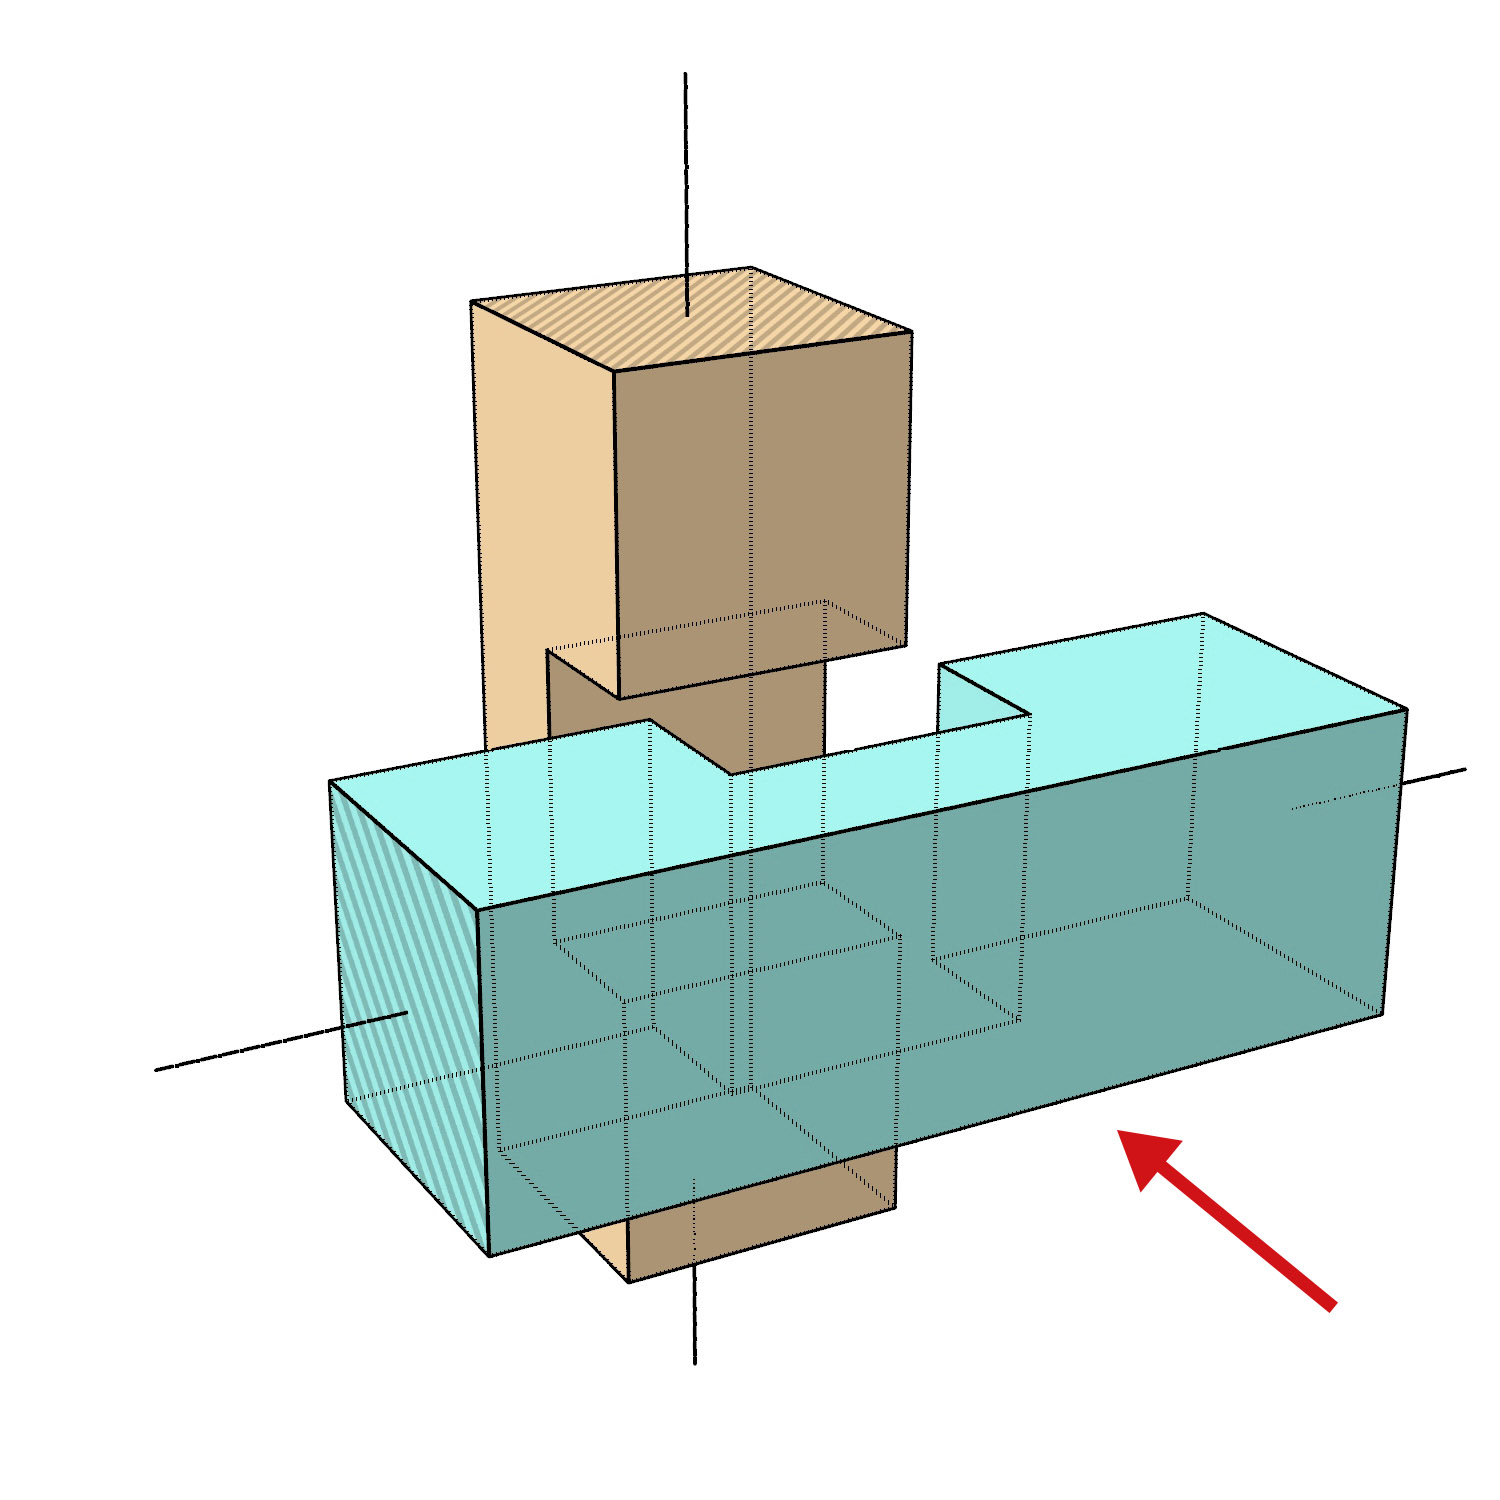
\includegraphics[width=\textwidth]{images/04-1+2/CrossLap_6_witharrows.jpg}
         \caption{Lap Joint (Cross shape)}
         \label{fig:common-joints-crosslap}
     \end{subfigure}
     \hfill
     \begin{subfigure}[b]{0.32\textwidth}
         \centering
         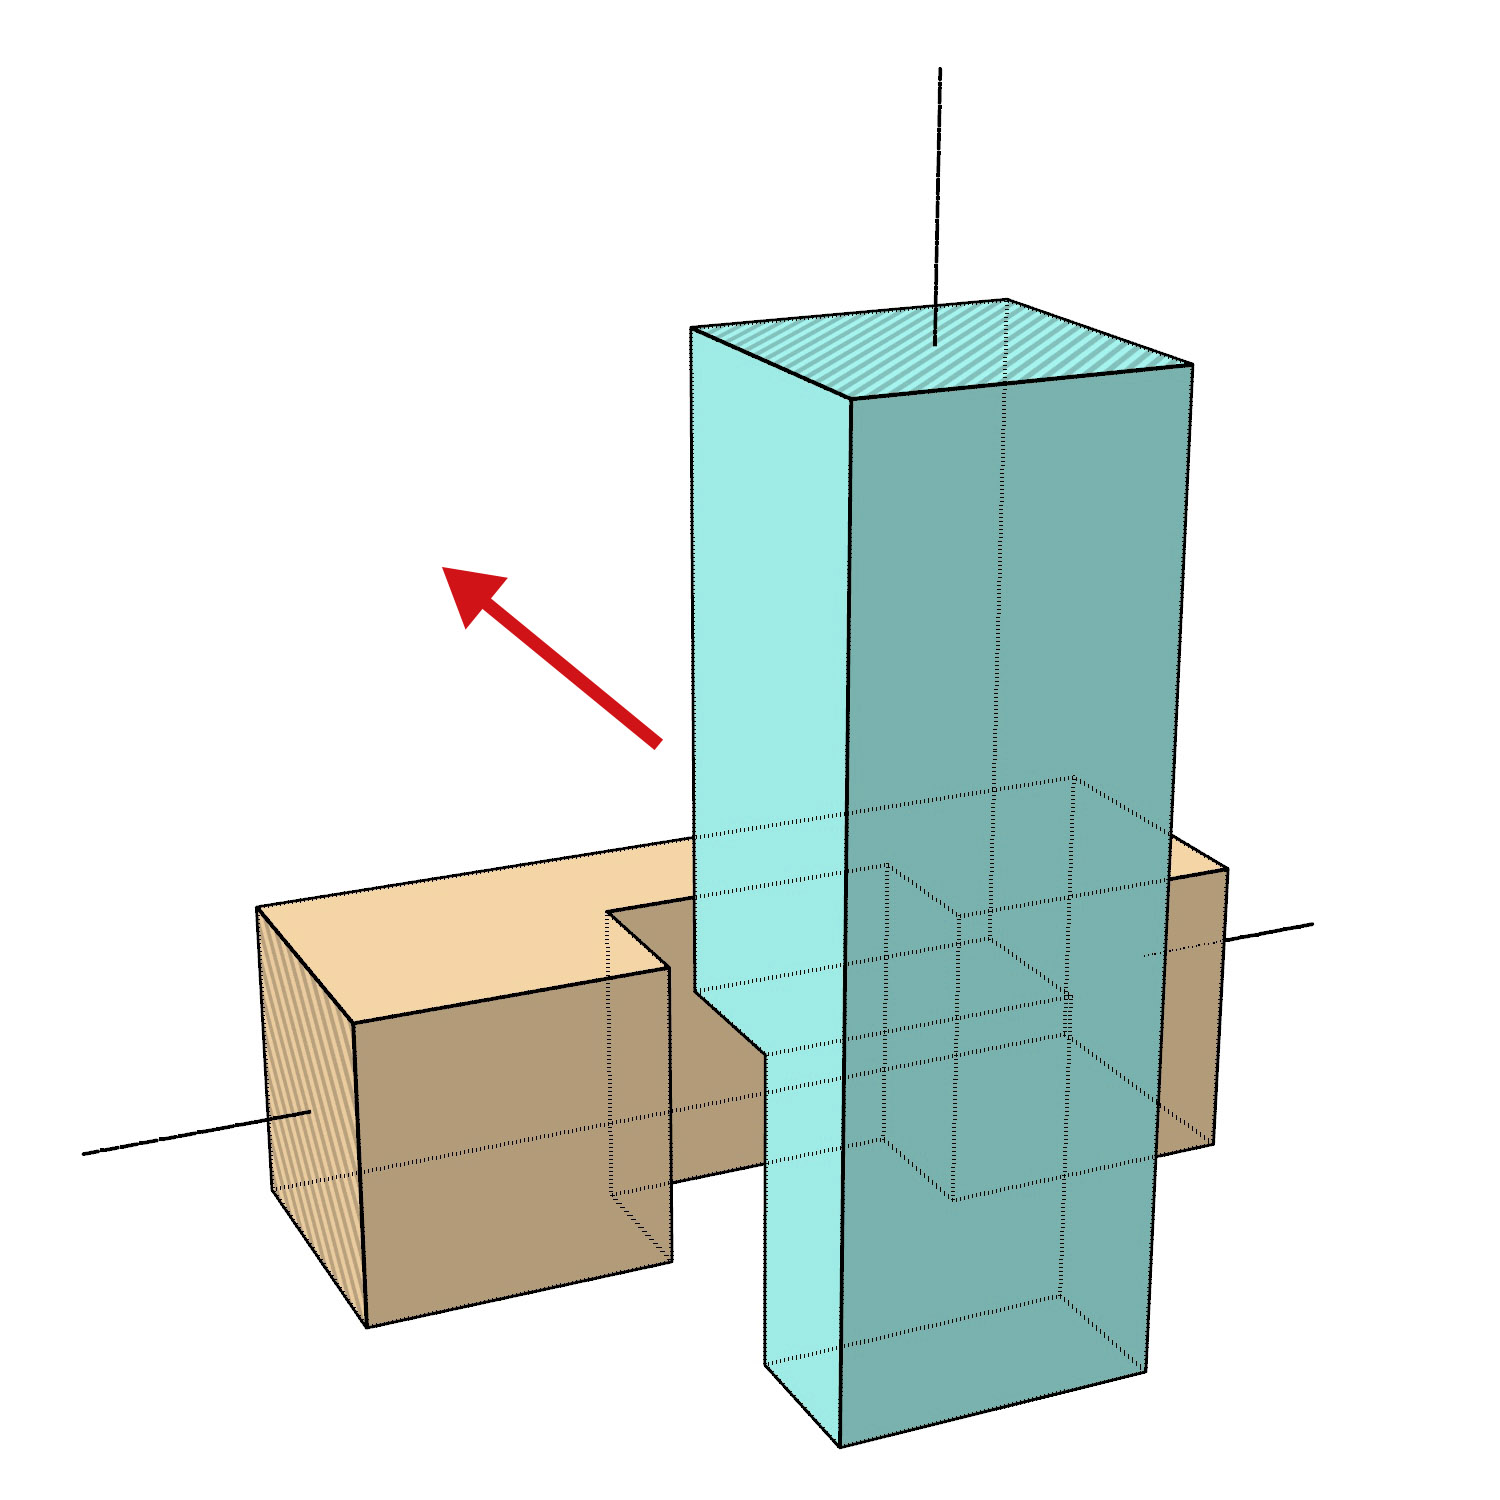
\includegraphics[width=\textwidth]{images/04-1+2/TeeLap_6_witharrows.jpg}
         \caption{Lap Joint (Tee shape)}
         \label{fig:common-joints-teelap}
     \end{subfigure}
     \hfill
     \begin{subfigure}[b]{0.32\textwidth}
         \centering
         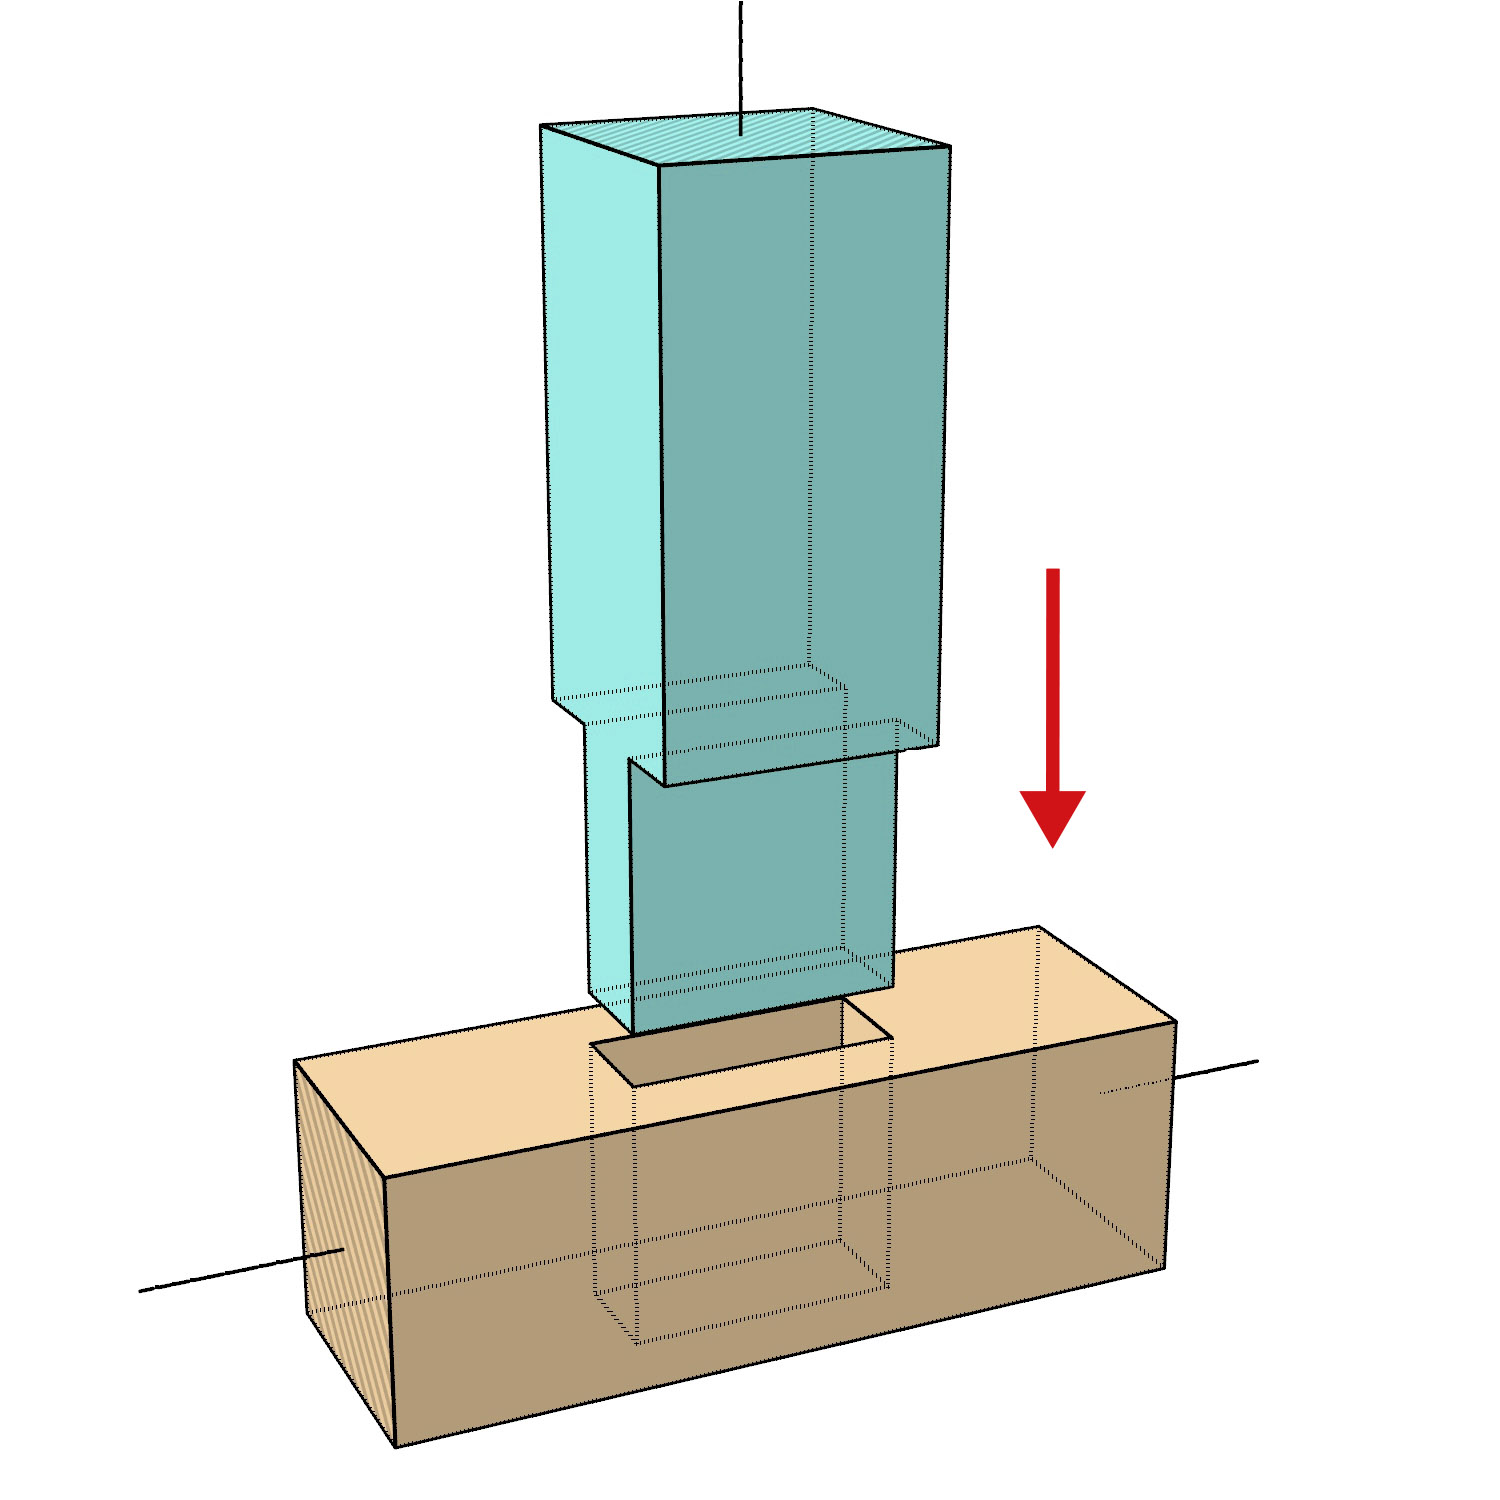
\includegraphics[width=\textwidth]{images/04-1+2/Tenon_6_witharrows.jpg}
         \caption{Mortise Tenon Joint}
         \label{fig:common-joints-mortisetenon}
     \end{subfigure}
     \caption{Diagrams of common integral timber joints used in timber frame construction}
     \label{fig:three-common-joints}
\end{figure}

\subsection{Joint Tightness}
\label{subsection:exploration-1-joint-tightness}

For the purpose of developing robotic actuators, it is necessary to quantify the force needed to assemble the lap joint. Based on my own carpentry experience and the report from a related timber joint study (Robeller et al., 2017), the assembly force for an architectural scale joint is not only related to but also highly sensitive to the fit of joint geometry. Due to the lack of relevant literature, a test was conducted to identify the force required for different joint tightness.

\subsubsection{Tightness Measurement Setup}

The samples to be tested consisted of 6 pieces of joint samples (six half sides). In order to maximise the data being collected, each joint-half was paired with others and test assembled with one another in all possible combinations, providing 15 test pairs.

The samples are made with construction grade spruce with 80mm x 80mm cross section\footnote{Note that the sample size is 80mm x 80mm, but the timber intended for this thesis is 100mm x 100mm. However, the result is good enough for the purpose of specifying the clamping force.} with a construction grade plane finish.
The shoulders of each joint were cut manually with a Japanese pull saw. The cheek width (C) and notch width (N) are measured after the joint is cut (see Figure \ref{fig:lap-joint-assembly-rubbing-before}), multiple points were measured with a caliper with 0.01mm resolution and their mean value is recorded.

\begin{figure}
    \centering
    \begin{subfigure}[b]{0.49\textwidth}
        \centering
        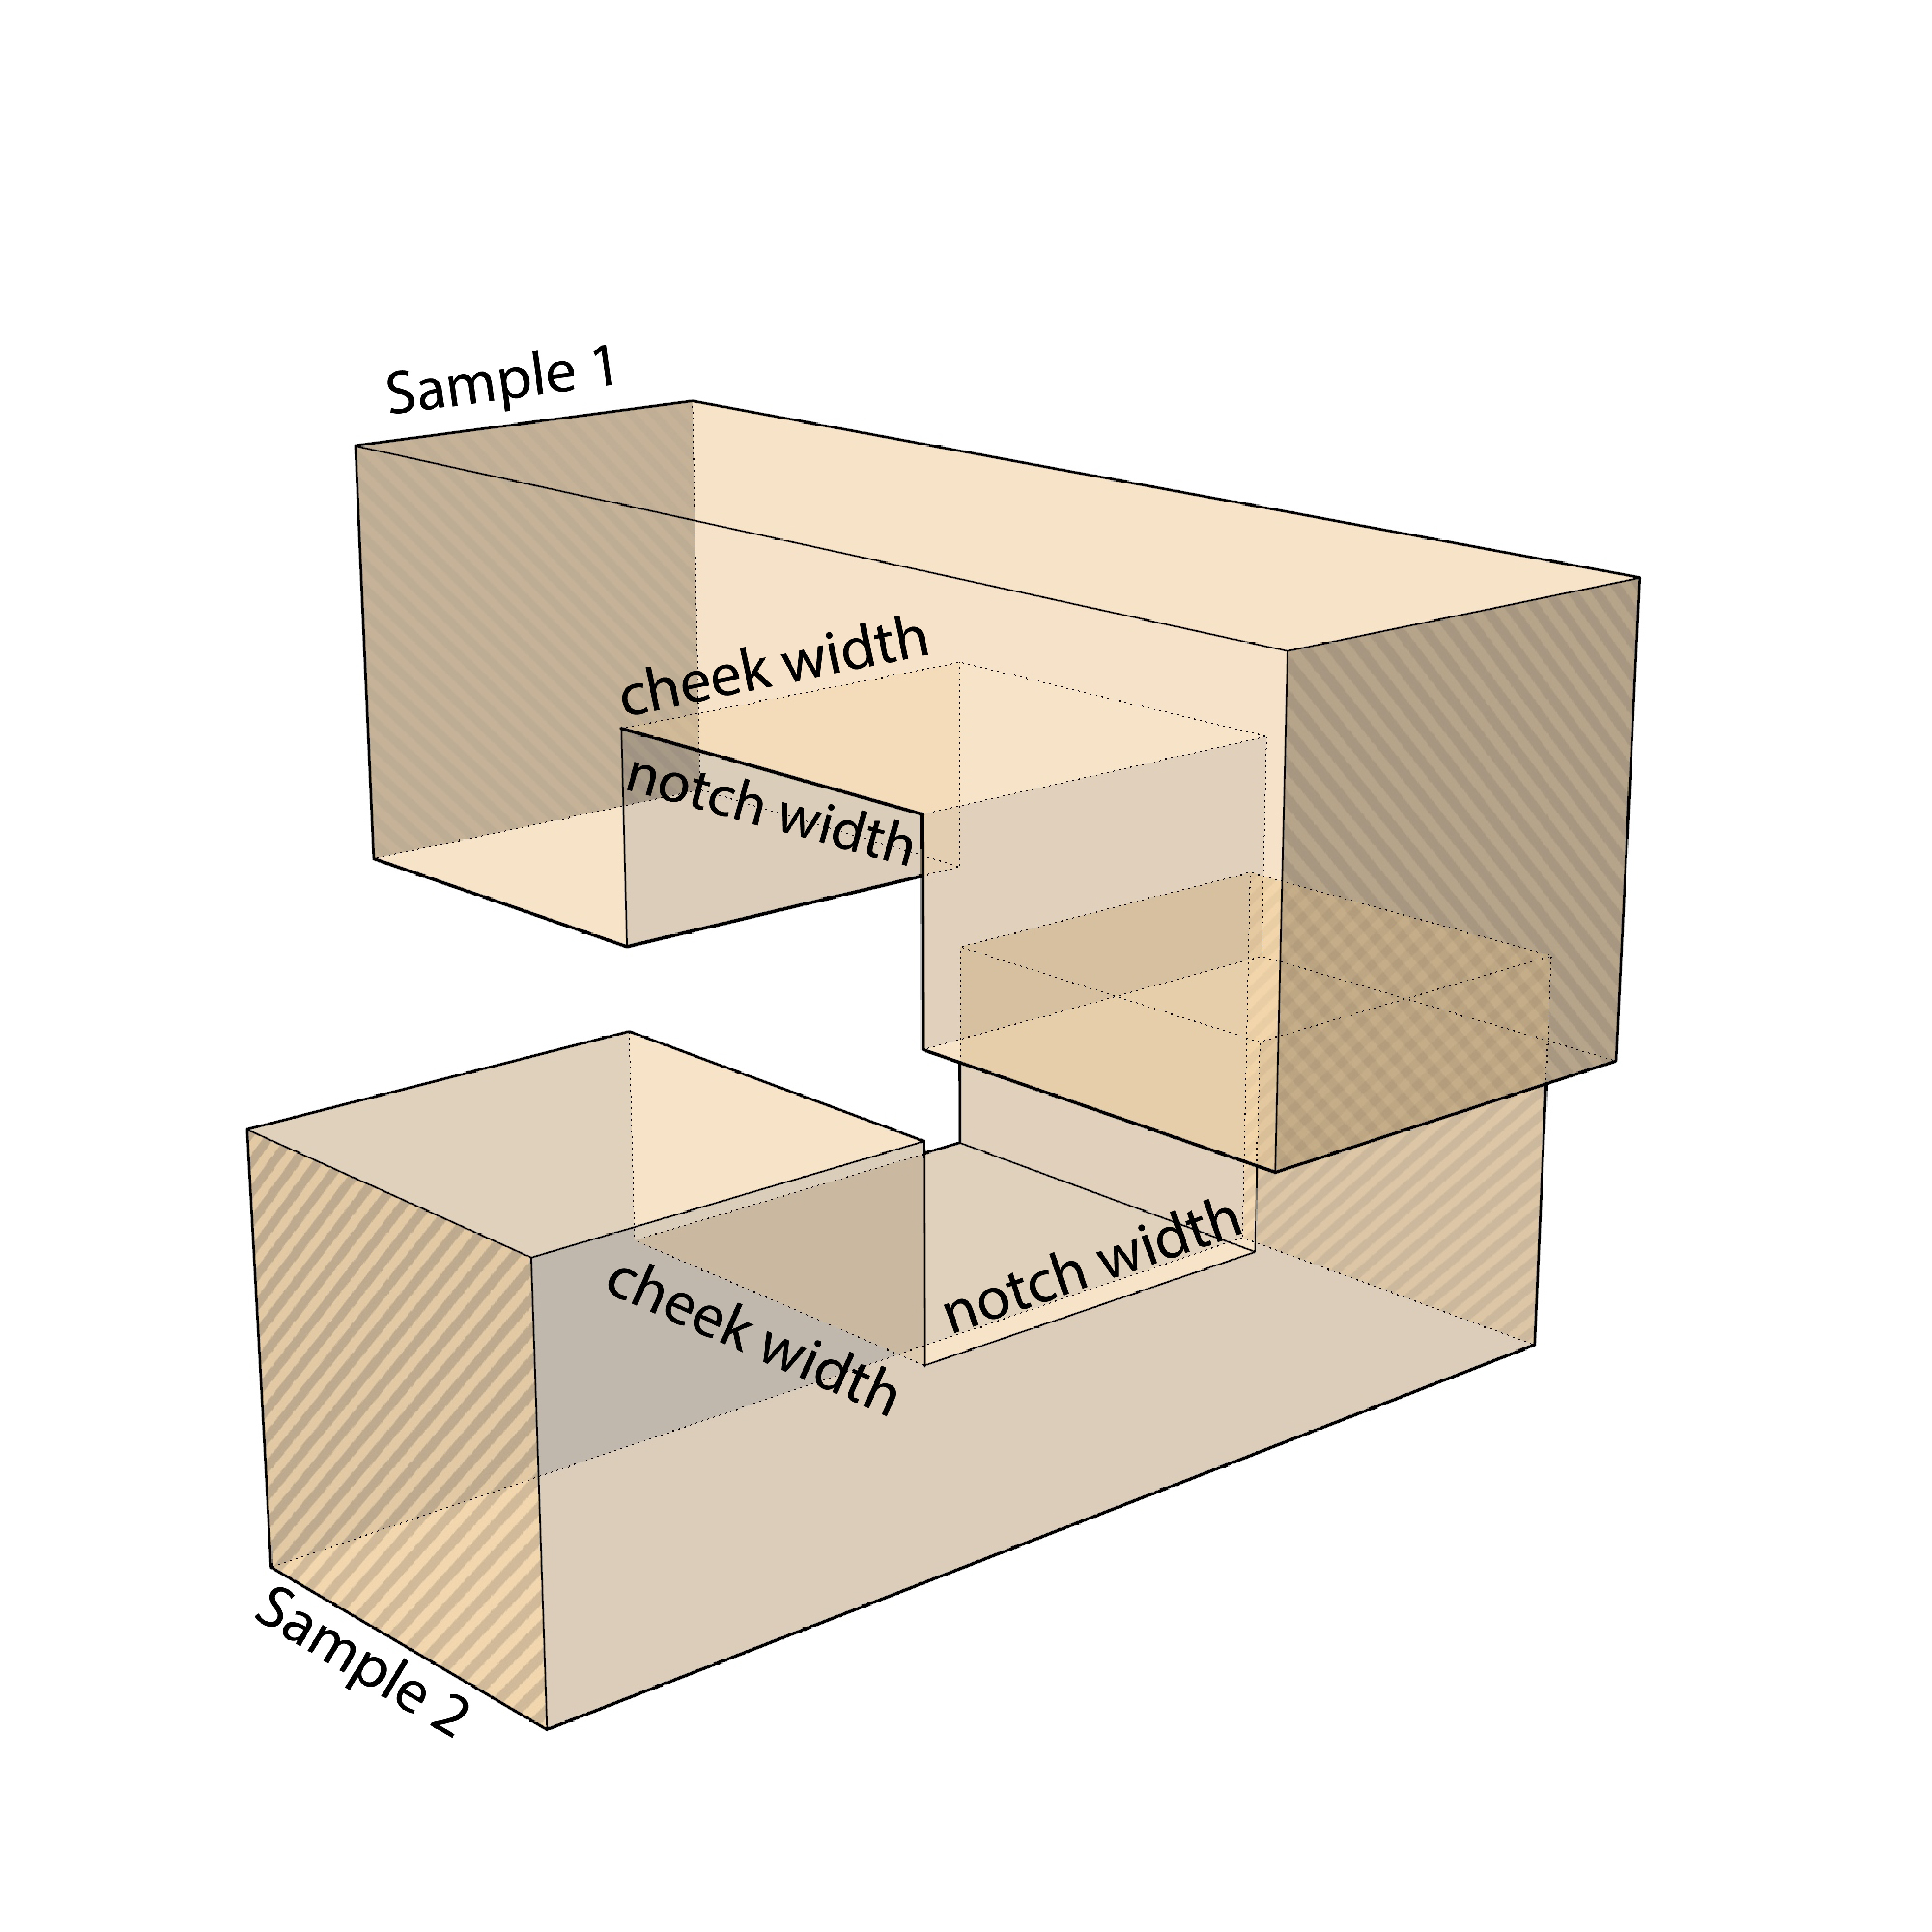
\includegraphics[width=\textwidth]{images/04-1+2/tightness-measurement.jpg}
        \caption{Before Assembly}
        \label{fig:lap-joint-assembly-rubbing-before}
    \end{subfigure}
    \hfill
    \begin{subfigure}[b]{0.49\textwidth}
        \centering
        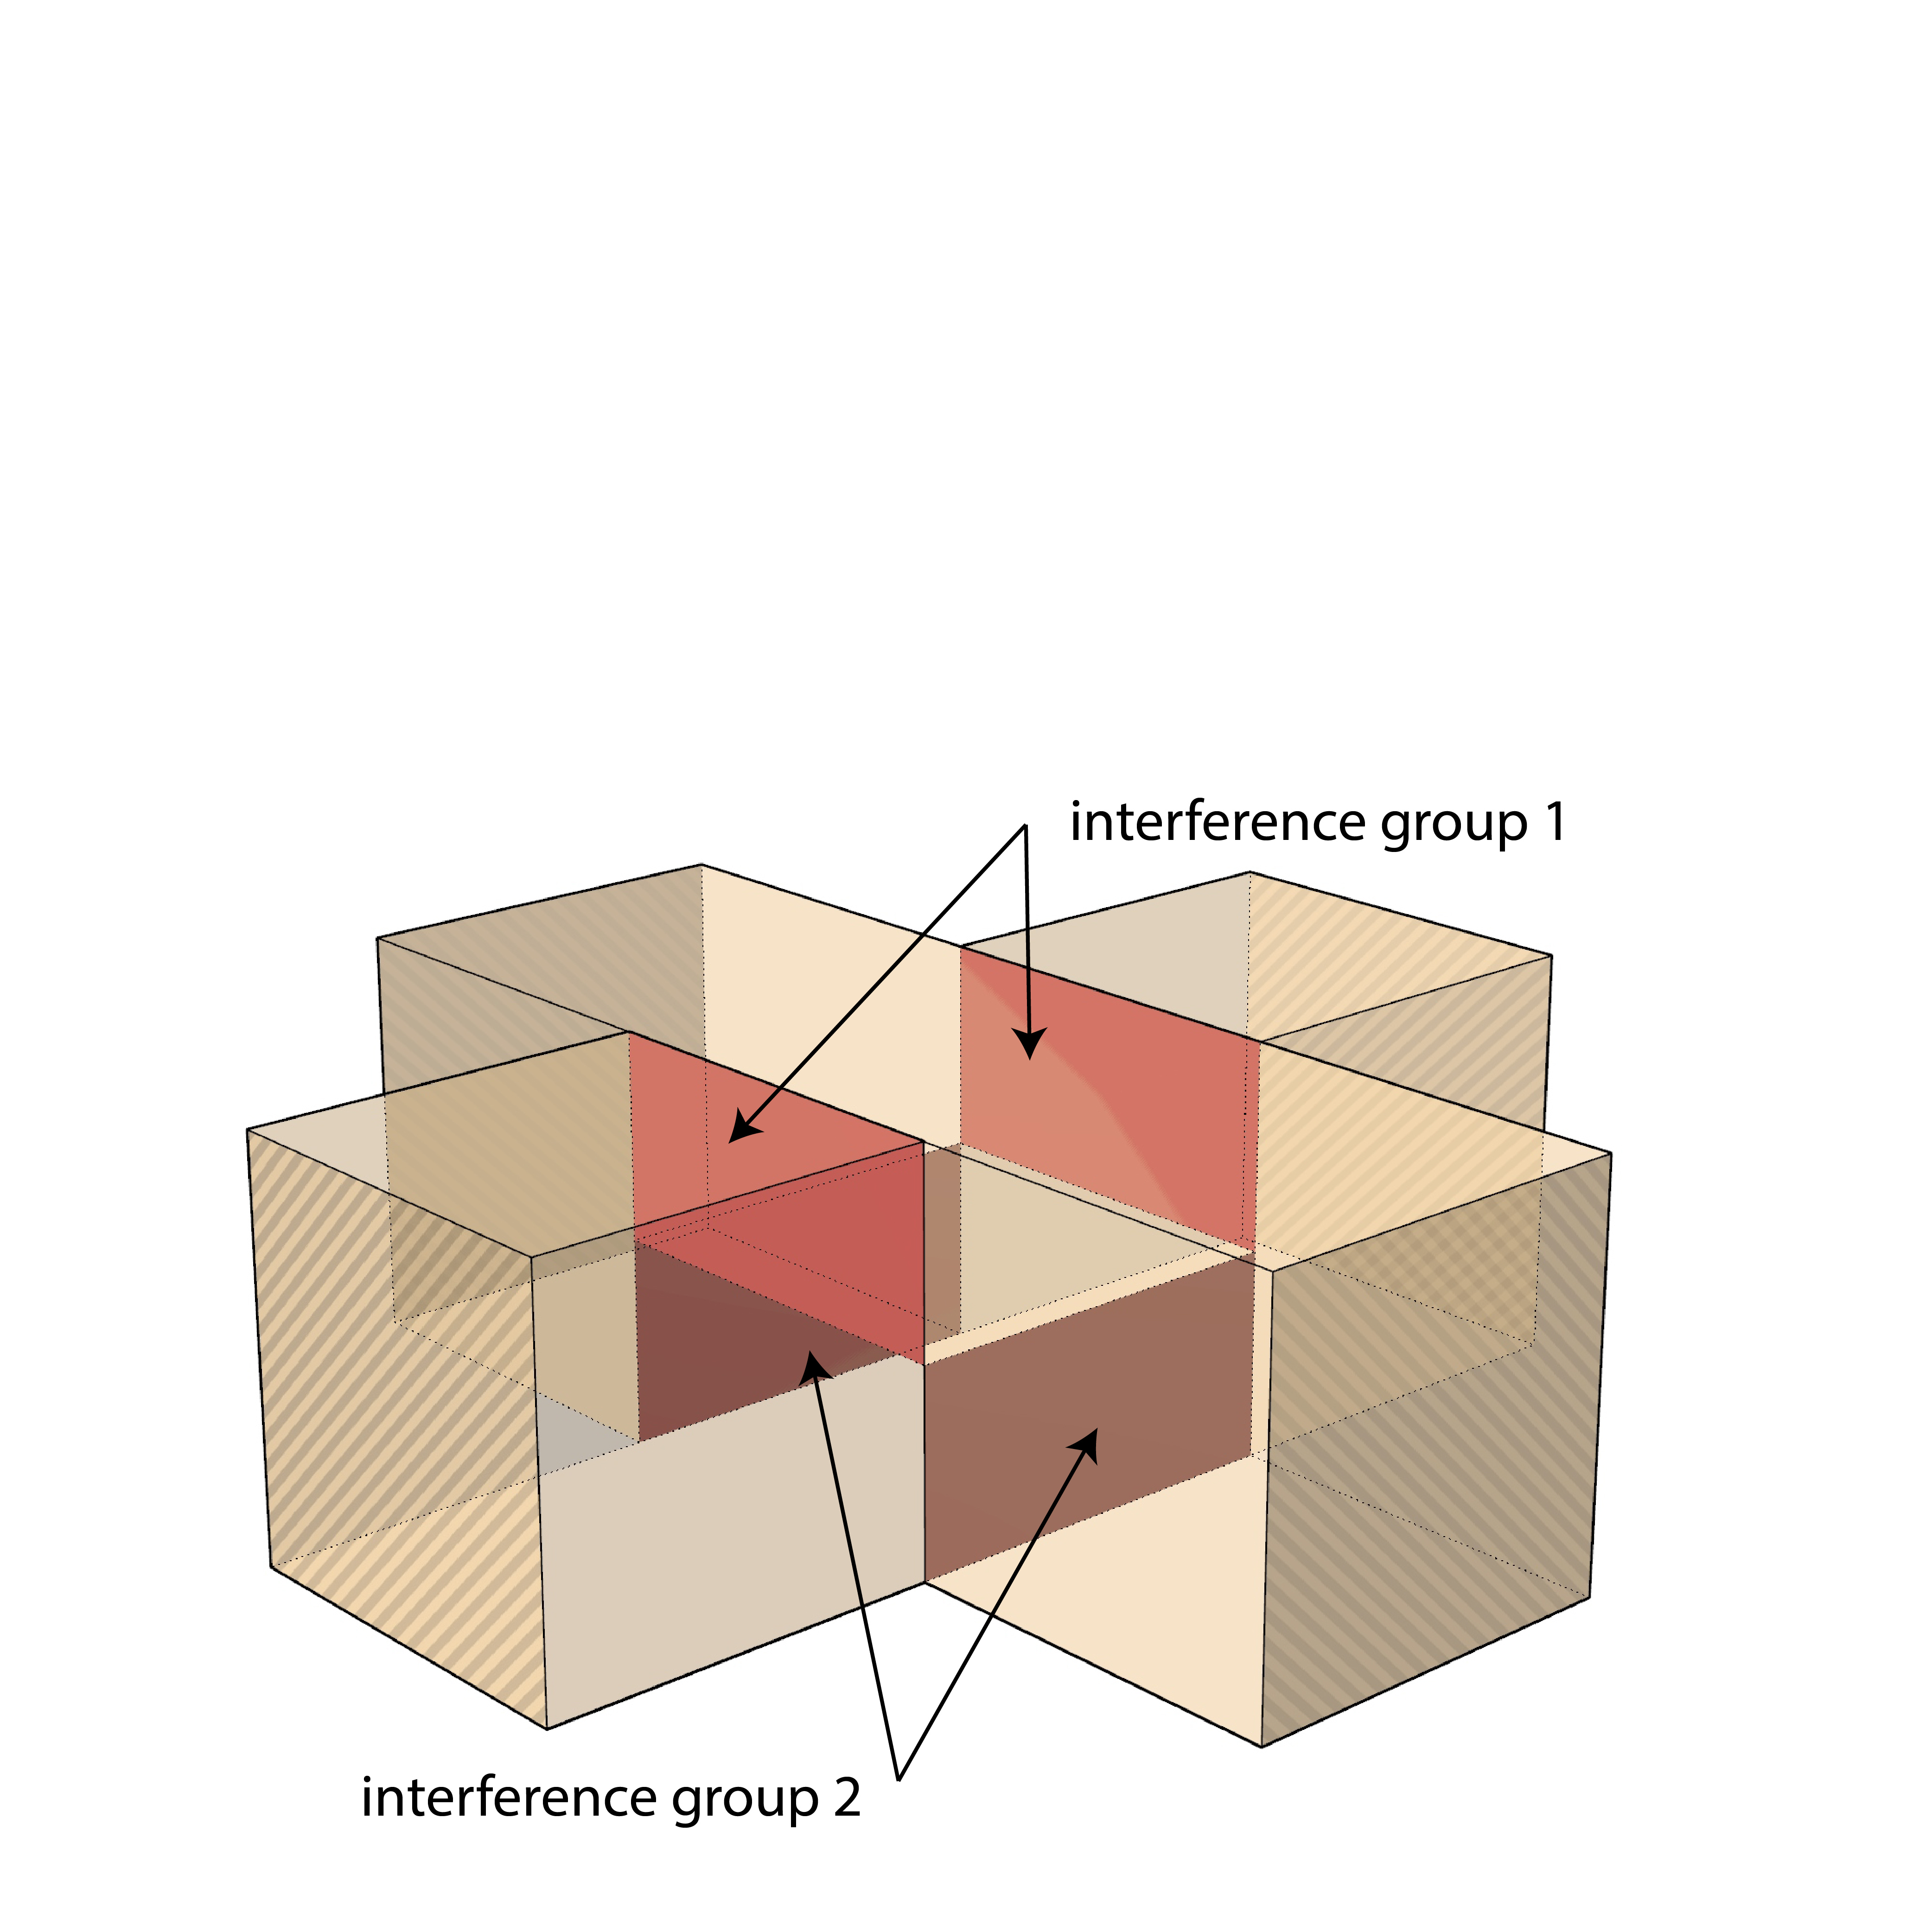
\includegraphics[width=\textwidth]{images/04-1+2/tightness-rubsurface.jpg}
        \caption{After Assembly}
        \label{fig:lap-joint-assembly-rubbing-after}
    \end{subfigure}
    \caption{Diagram showing surfaces (red) that are in rubbing contact during assembly}
    \label{fig:lap-joint-assembly-rubbing}
\end{figure}


Figure \ref{fig:lap-joint-assembly-rubbing-after} shows four surfaces that were expected to be in tight rubbing contact, contributing to assembly resistance. These surfaces come in two interference groups (IG). Interference for each group can be computed by the following formula. Note that the value is positive when there is interference. The case where the joint is loose, it is assumed to have 0 interference. 

Interference of IG 1 = $max( C (Sample 1) - N (Sample 2), 0)$\\
Interference of IG 2 = $max( C (Sample 2) - N (Sample 1), 0)$

The mean interference between the two groups is used as an indication of the tightness of a joint. The larger the interference, the tight the joint. Figure \ref{fig:interference-amount} shows the computed mean interference for each Interference Group. The force-measurement setup consists of a manually actuated carpentry clamp compressing on a digital load cell which compresses the lap joint (see Figure \ref{fig:interference-measurement-setup}). The force during the assembly was logged and filtered and the maximum value was taken to represent the assembly force of the sample. Care was taken to not completely close the joint to ensure that the measured force was representing the kinematic part of the closure. If the cheeks of the lap joint were in contact, the measurement would be related to the stall force.

\begin{figure}
    \centering
    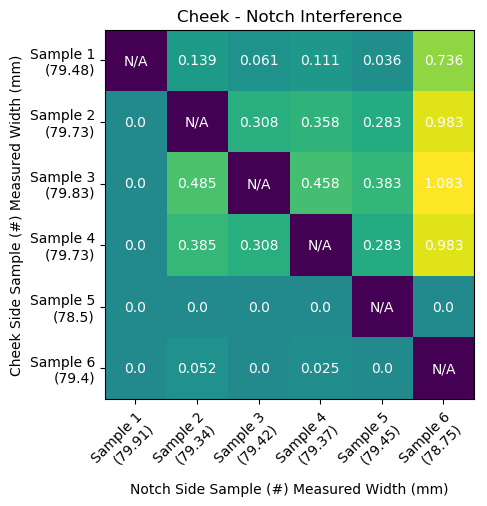
\includegraphics[width=0.6\textwidth]{images/04-1+2/tightness-pairwise-size.png}
    \caption{Amount of interference (mm) between between the sample pair}
    \label{fig:interference-amount}
\end{figure}

\begin{figure}
    \centering
    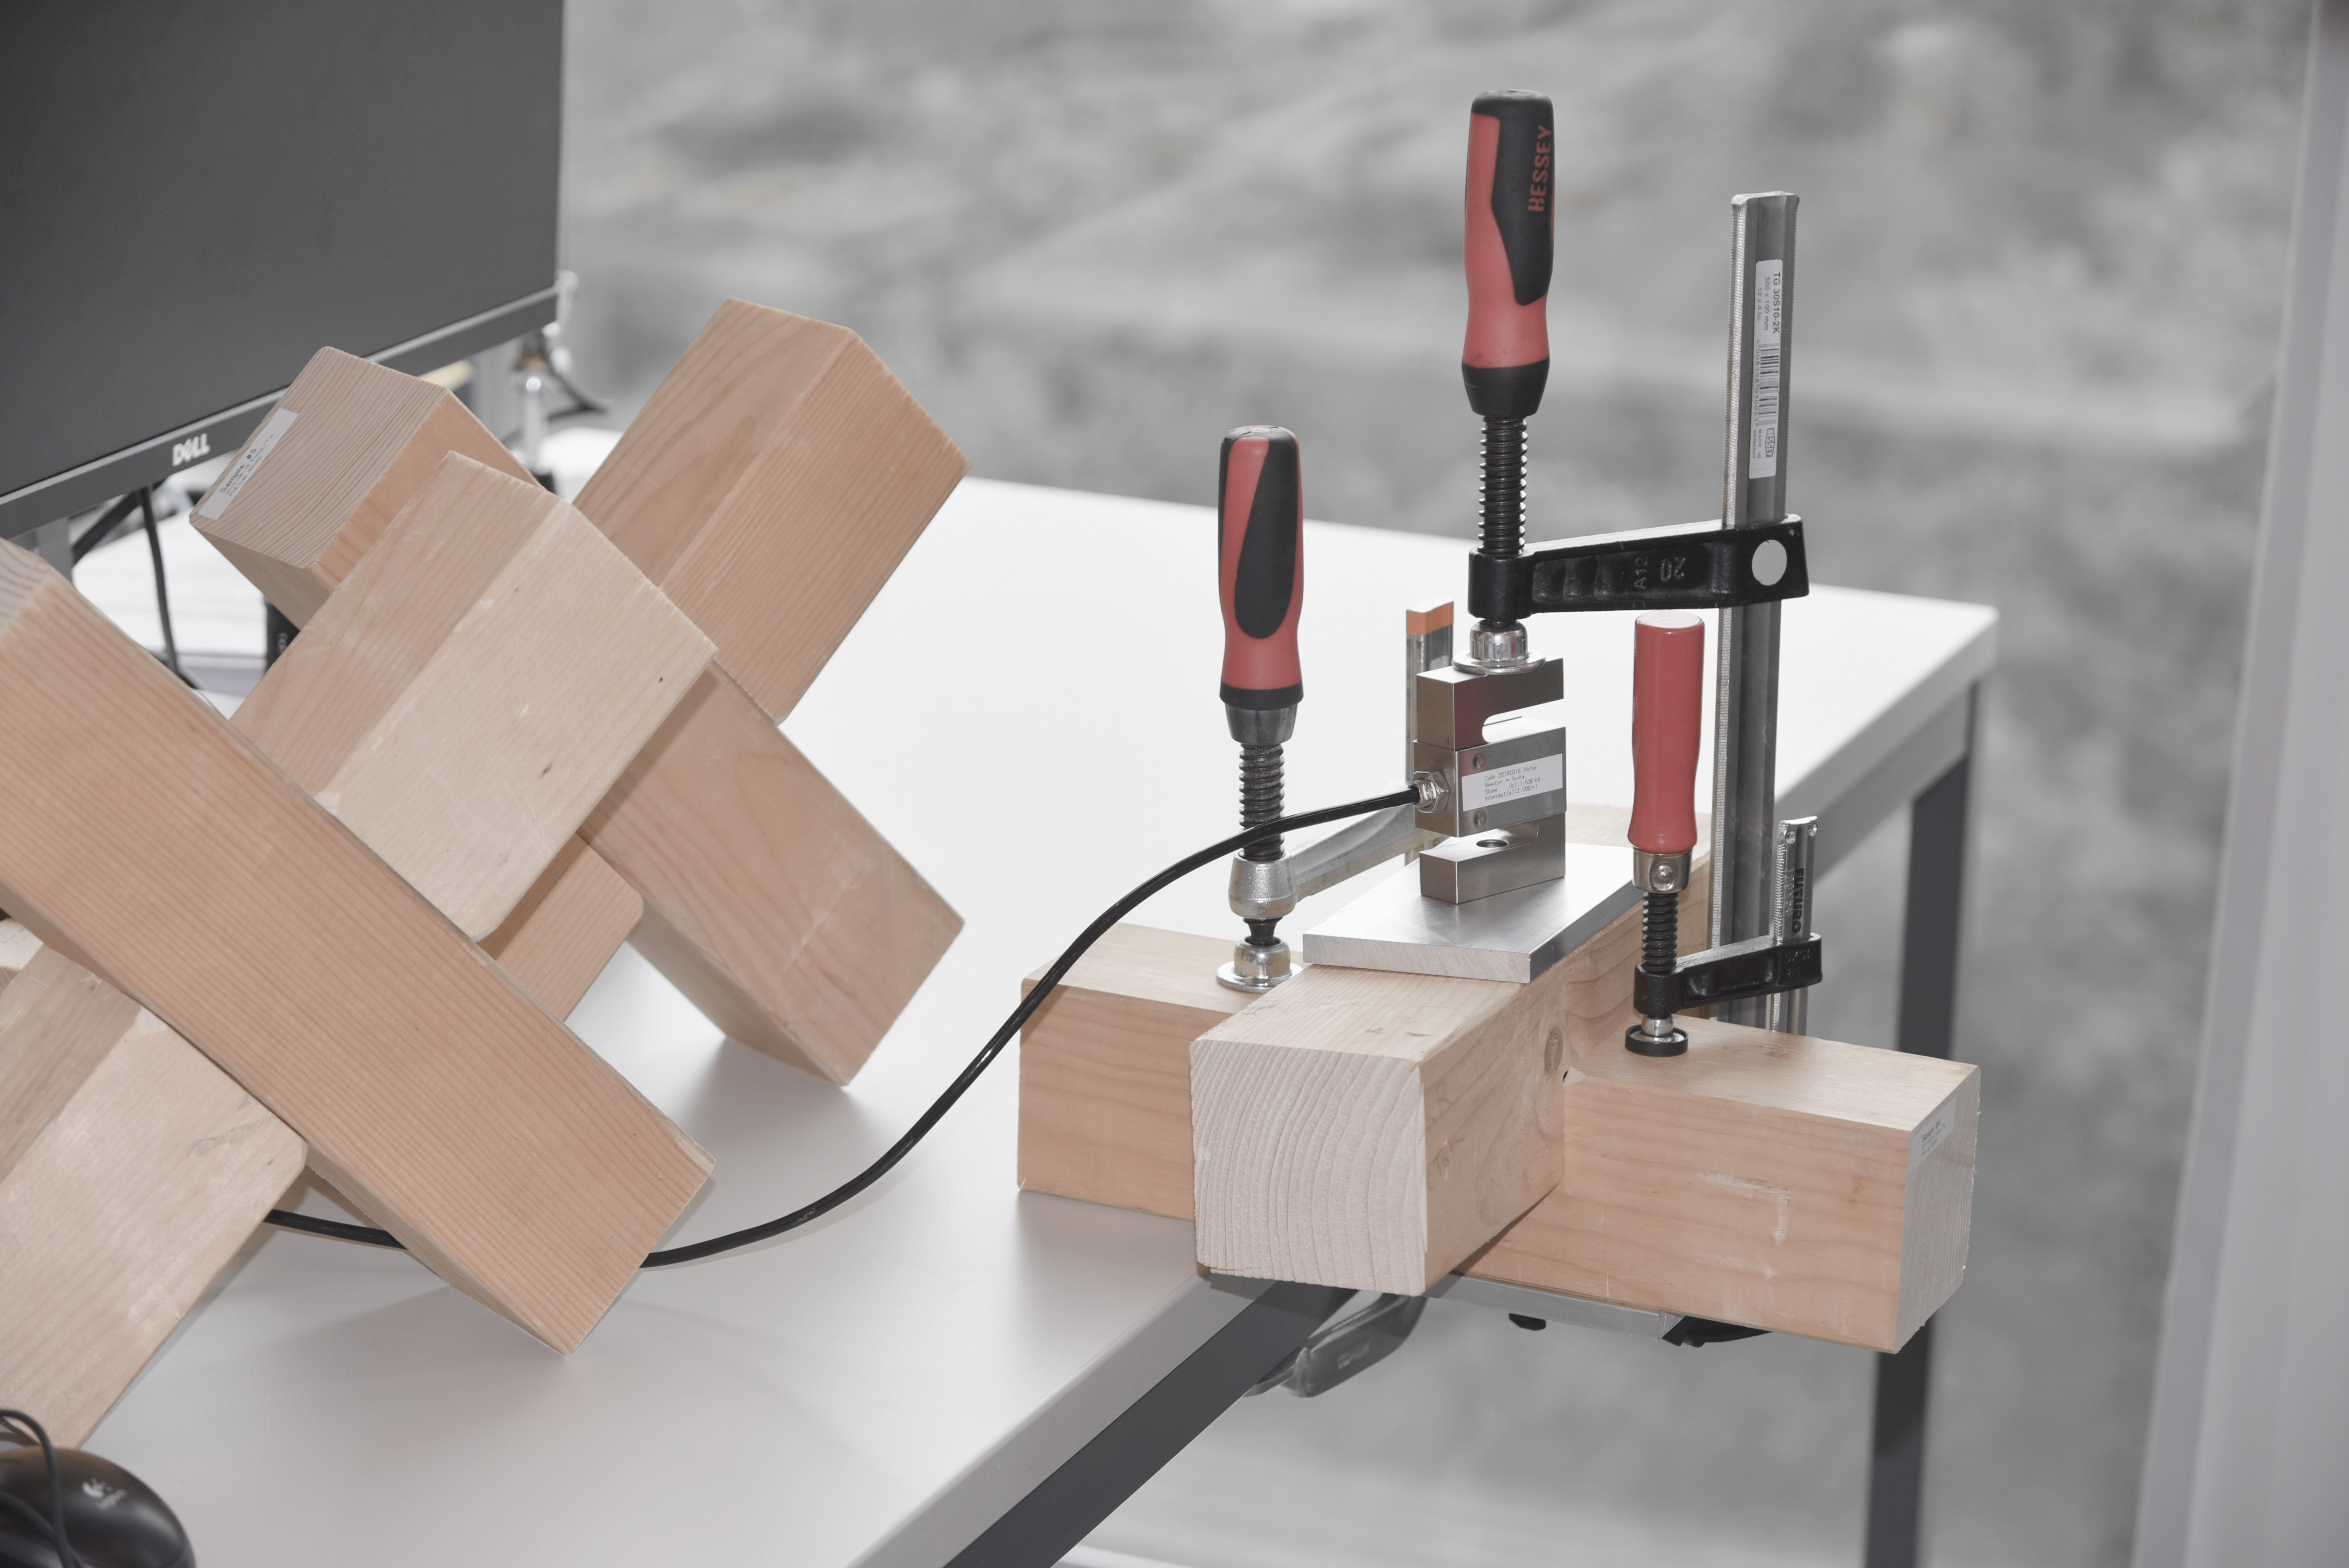
\includegraphics[width=0.99\textwidth]{images/04-1+2/setup.jpg}
    \caption{Setup for measuring closure force of lap joint samples}
    \label{fig:interference-measurement-setup}
\end{figure}

\subsubsection{Results and Conclusion about Joint Tightness}

Figure \ref{fig:tightness-measurement-pairwise} shows the pairwise force measurement result. Sample 1-4 was not measured because it had no friction at all. Sample 4-6 cannot be measured because it was too tight to begin any assembly motion. Figure \ref{fig:tightness-measurement-plot} shows the relationship between the mean interference (representing tightness) and the assembly force needed. 

\begin{figure}[H]
    \centering
    \begin{subfigure}[b]{0.40\textwidth}
        \centering
        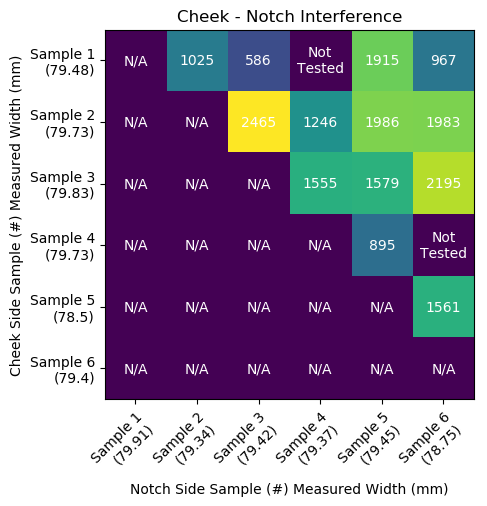
\includegraphics[width=\textwidth]{images/04-1+2/tightness-pairwise-result.png}
        \caption{Measurement result between pairs of samples}
        \label{fig:tightness-measurement-pairwise}
    \end{subfigure}
    \hfill
    \begin{subfigure}[b]{0.58\textwidth}
        \centering
        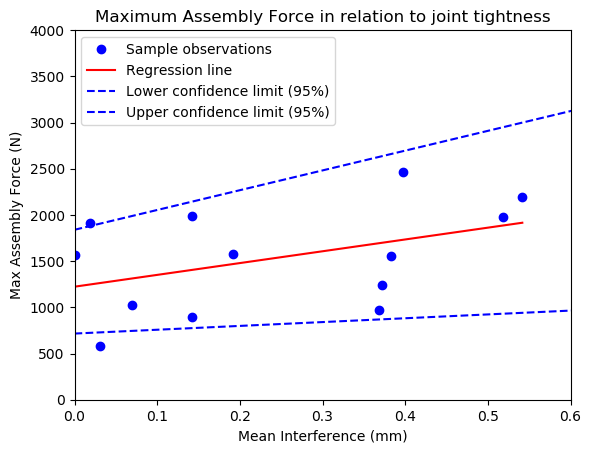
\includegraphics[width=\textwidth]{images/04-1+2/tightness-result-plot.png}
        \caption{Assembly force plot against interference between sample pairs}
        \label{fig:tightness-measurement-plot}
    \end{subfigure}
    \caption{Tightness measurement result}
    \label{fig:tightness-measurement-result}
\end{figure}

While it is not possible to conclude the correlation between the two quantities based on a few data samples, the test has shown a reasonable upper force limit for specifying the linear actuator. The forces measured are in the same order of magnitude as the number reported by a previous study (Robeller et al., 2017). For the purpose of designing the clamp actuator, the required clamping force was specified at 3000N. 

\section{Development}
\label{section:exploration-1-development}

\subsection{Lap Clamp CL1}
\label{subsection:exploration-1-lap-clamp-cl1-proof-of-concept}

The Lap Clamp CL1 was designed as a proof of concept clamp to demonstrate the robotic clamping action. The goal is to assemble a single orthogonal half-lap joint on a 100mm timber profile. 
In addition, it contains a spring-loaded parallel gripper mechanism to allow it to hang onto the structure. Figure \ref{fig:cl1-sketch} shows an early sketch of the clamp design, showing a U-shape configuration that surrounds a beam.

\begin{figure}
    \centering
    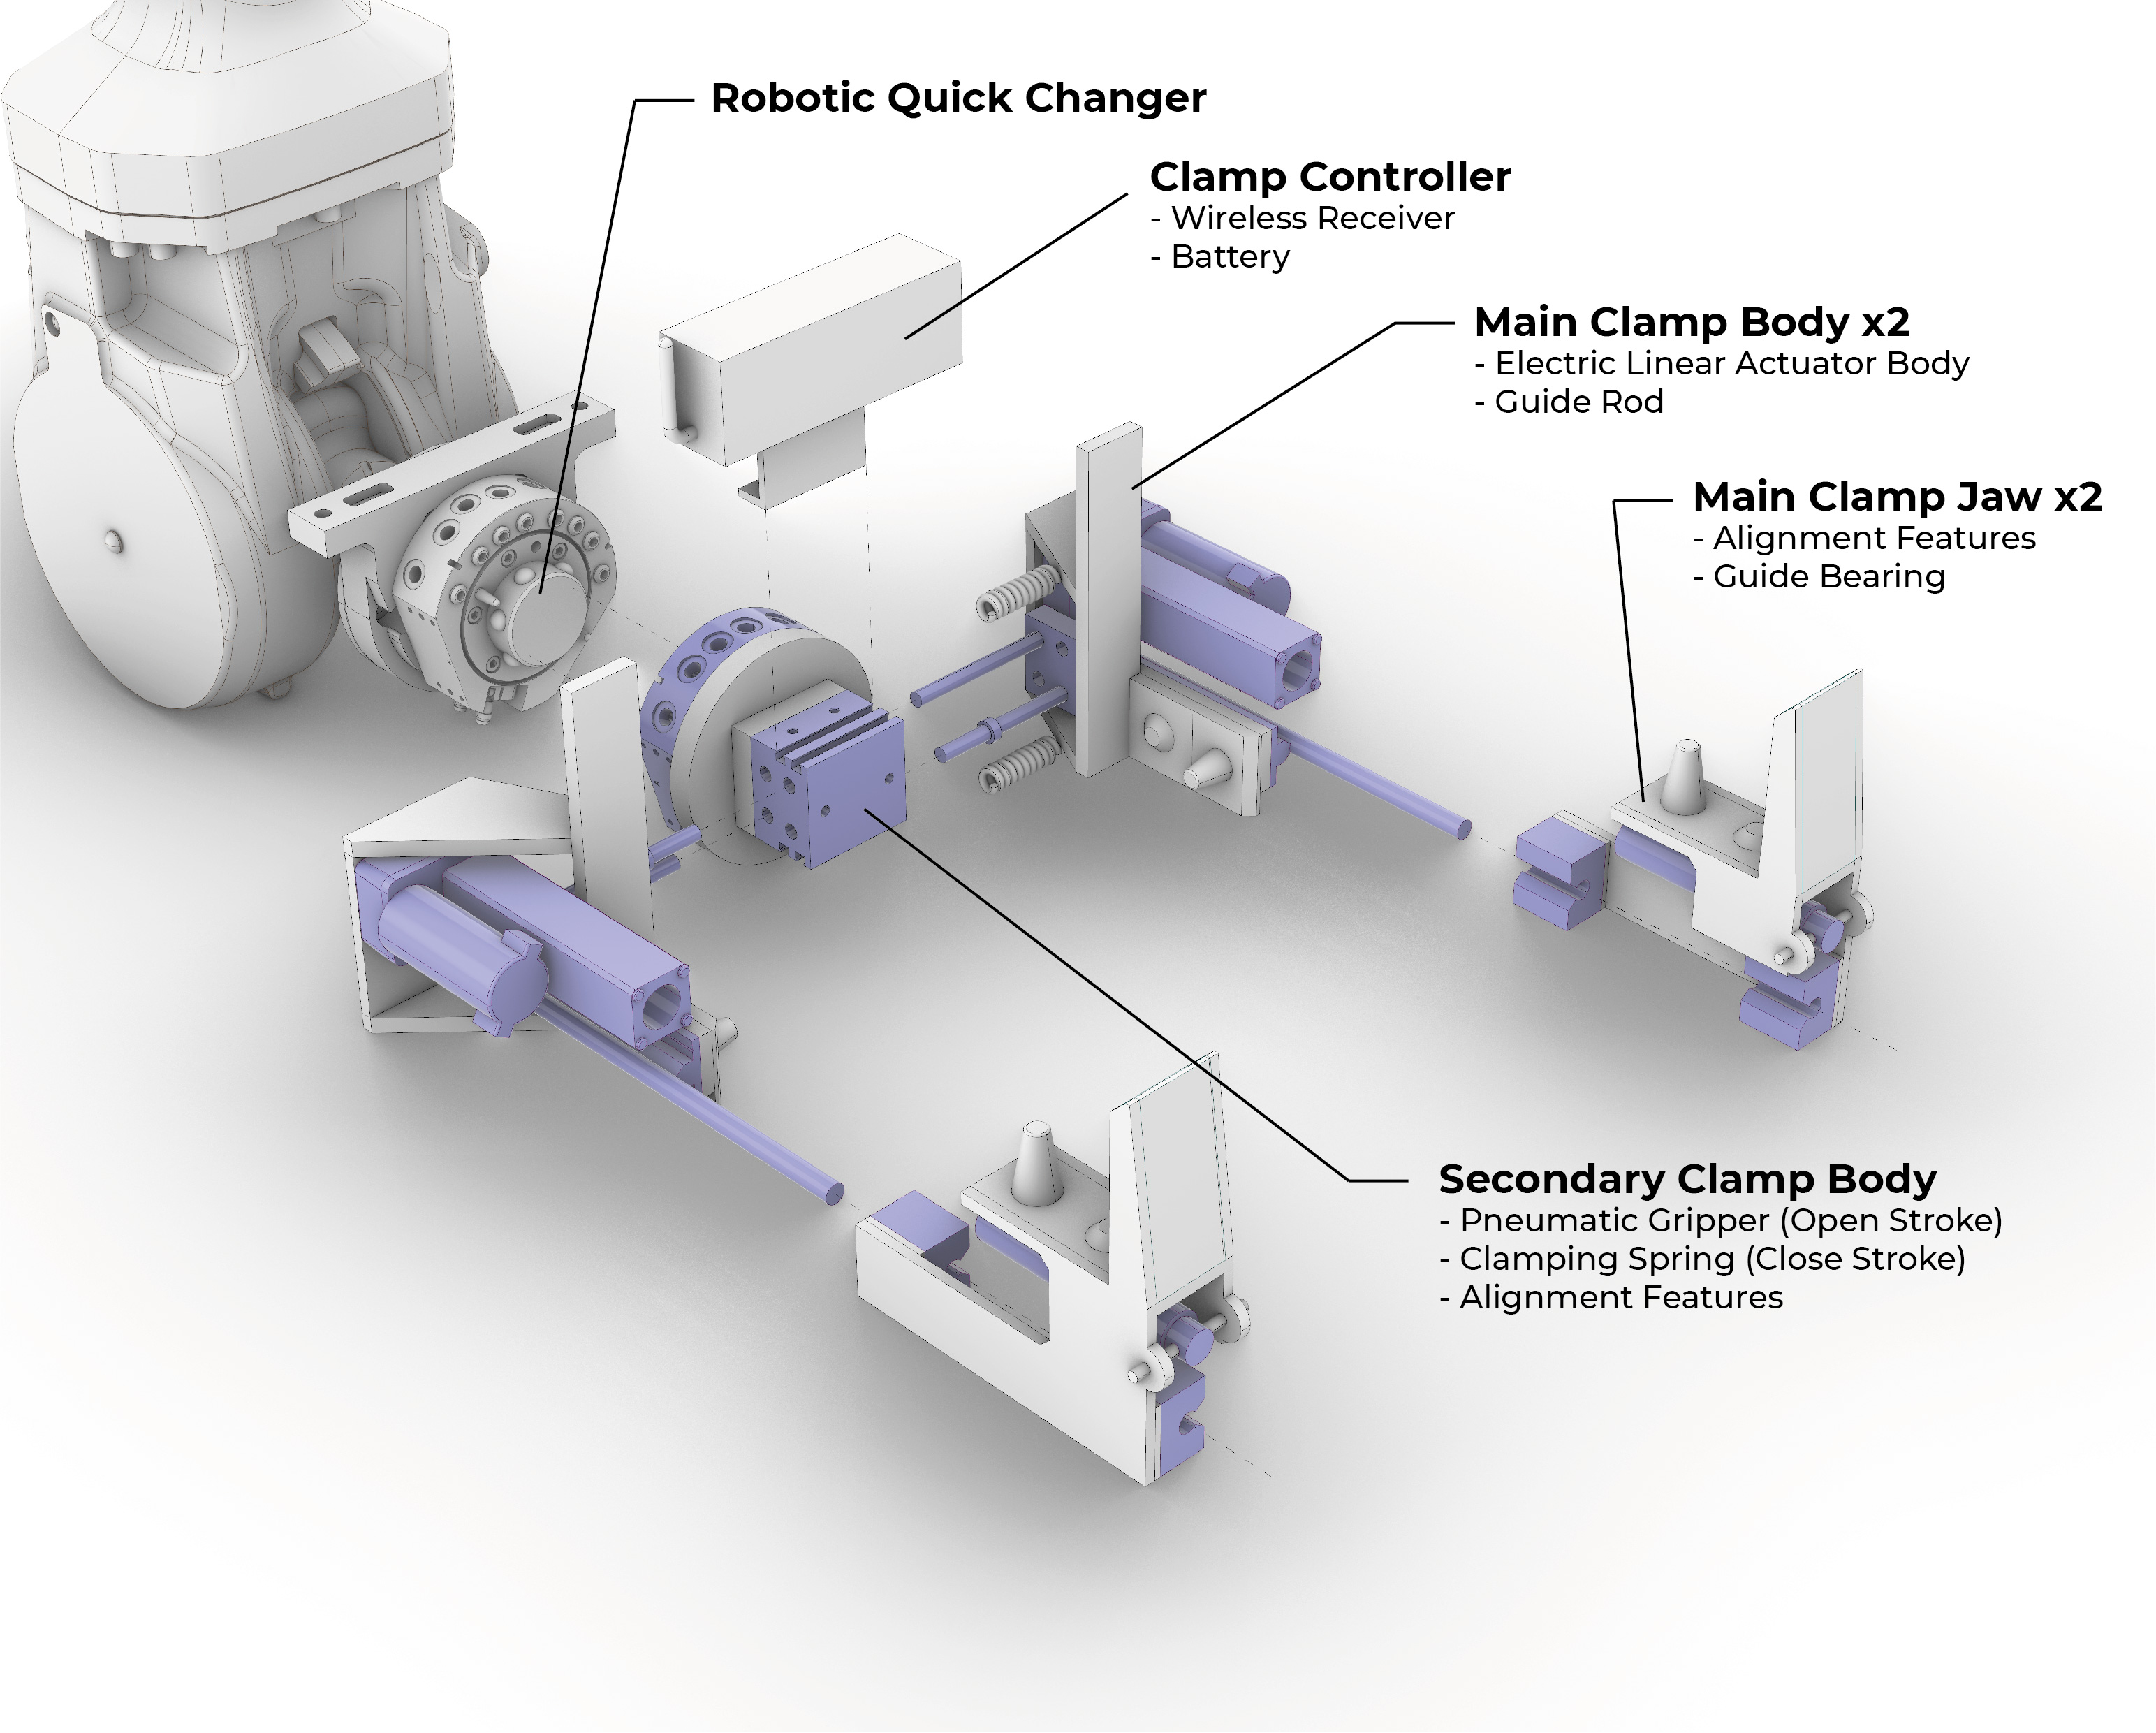
\includegraphics[width=0.99\textwidth]{images/04-3/cl1-exploded-diagram.jpg}
    \caption{Sketch drawing of the CL1 clamp design showing the U-shape configuration}
    \label{fig:cl1-sketch}
\end{figure}

\subsubsection{Linear Actuator and Jaw Design}
\label{subsubsection:exploration-1-linear-actuator-and-jaw-design}

The robotic clamp jaw is designed around a linear actuator typically used for movable furniture (see Figure \ref{fig:linear-actuator-cl1}), it has a compact design and is rated for 2000N of force at 5mm/s. Despite the force being lower than the 3000N requirement established in \noseeref{subsection:exploration-1-joint-tightness}, using two jaws combined would likely be sufficient to overcome the tightest joint. The motor contains a 2-channel hall effect encoder fixed to the motor shaft, this is needed for closed loop position control \seeref{subsubsection:exploration-1-bang-bang-motion-control}. 

\begin{figure}[hb!]
    \centering
    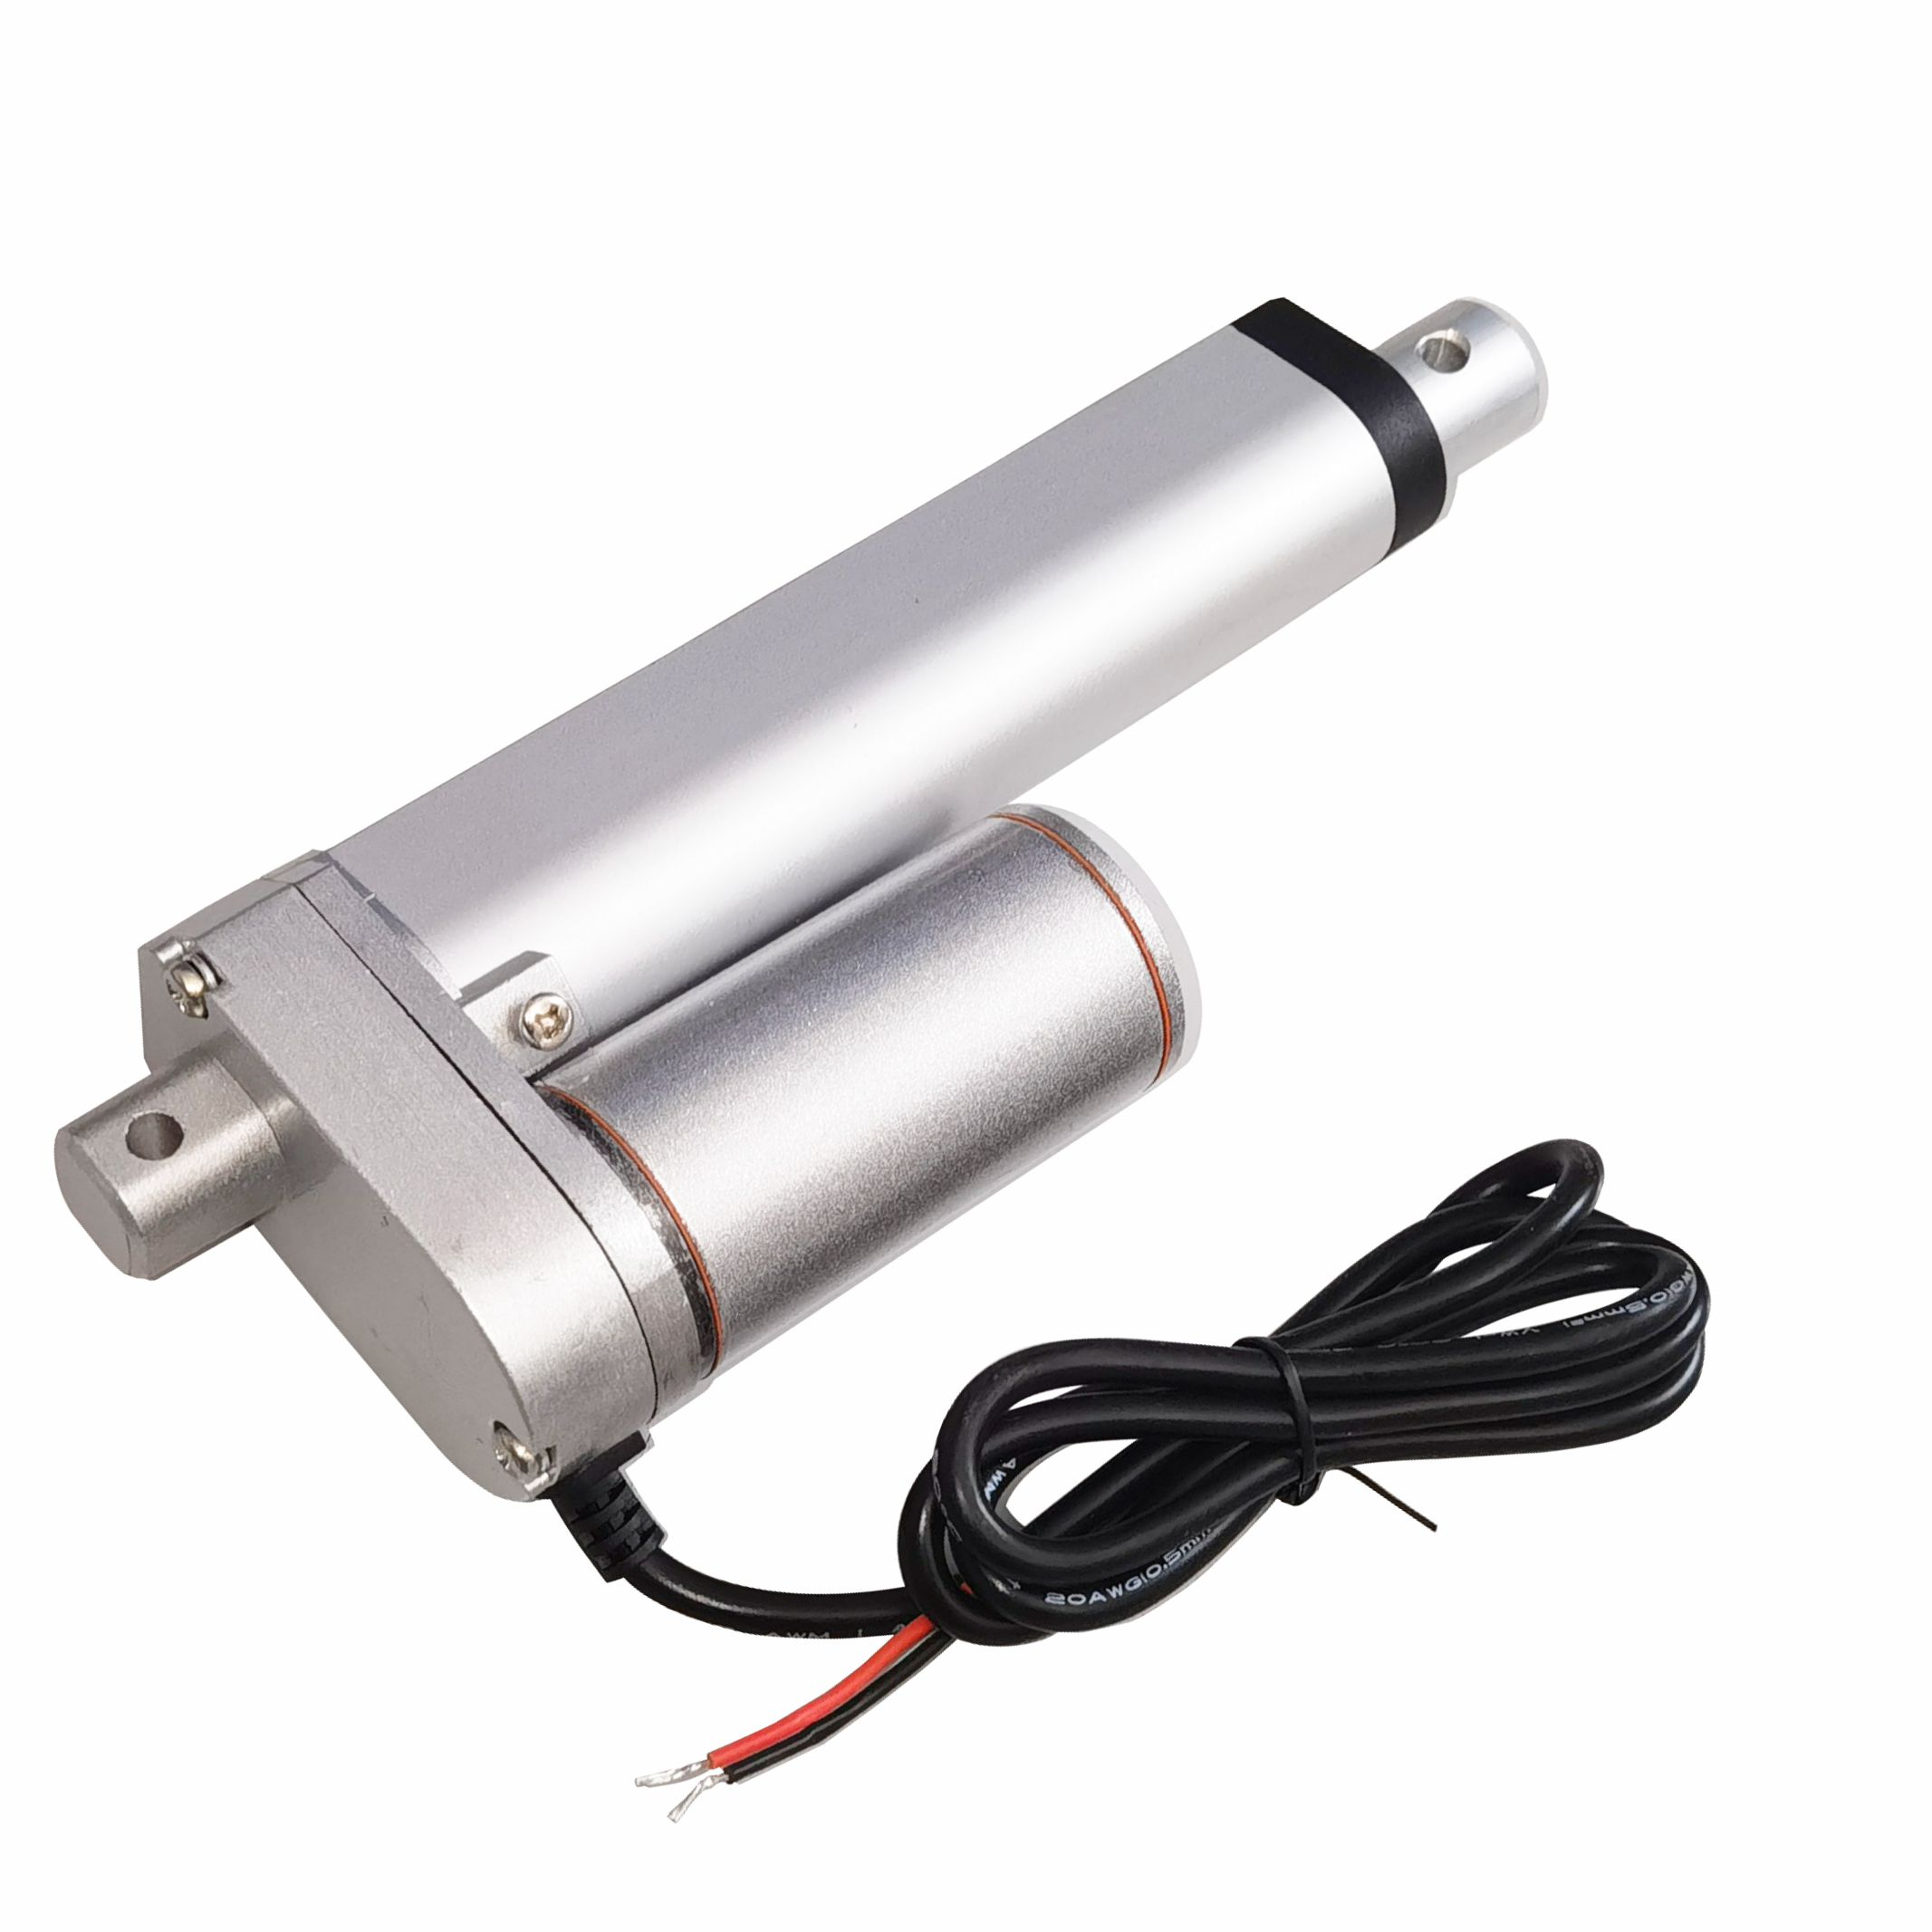
\includegraphics[width=0.99\textwidth]{images/04-3/cl1-linearactuator.jpg}
    \caption{Linear actuator used in the CL1 clamp}
    \label{fig:linear-actuator-cl1} 
\end{figure}

The clamp jaw is made from aluminium plates bolted together. It has two open-type bronze linear bushing paired with a 12mm round shaft to act as linear motion guide. The bronze bearing was chosen over ball-type linear bearings to maximise load capacity. The front side of the actuator is mounted with an in-line load cell for collecting force data for analysis. Figure \ref{fig:cl1-clamp-jaw} shows the detached clamp jaw from the guide shaft and linear actuator. 

\begin{figure}
    \centering
    \begin{subfigure}[b]{0.49\textwidth}
        \centering
        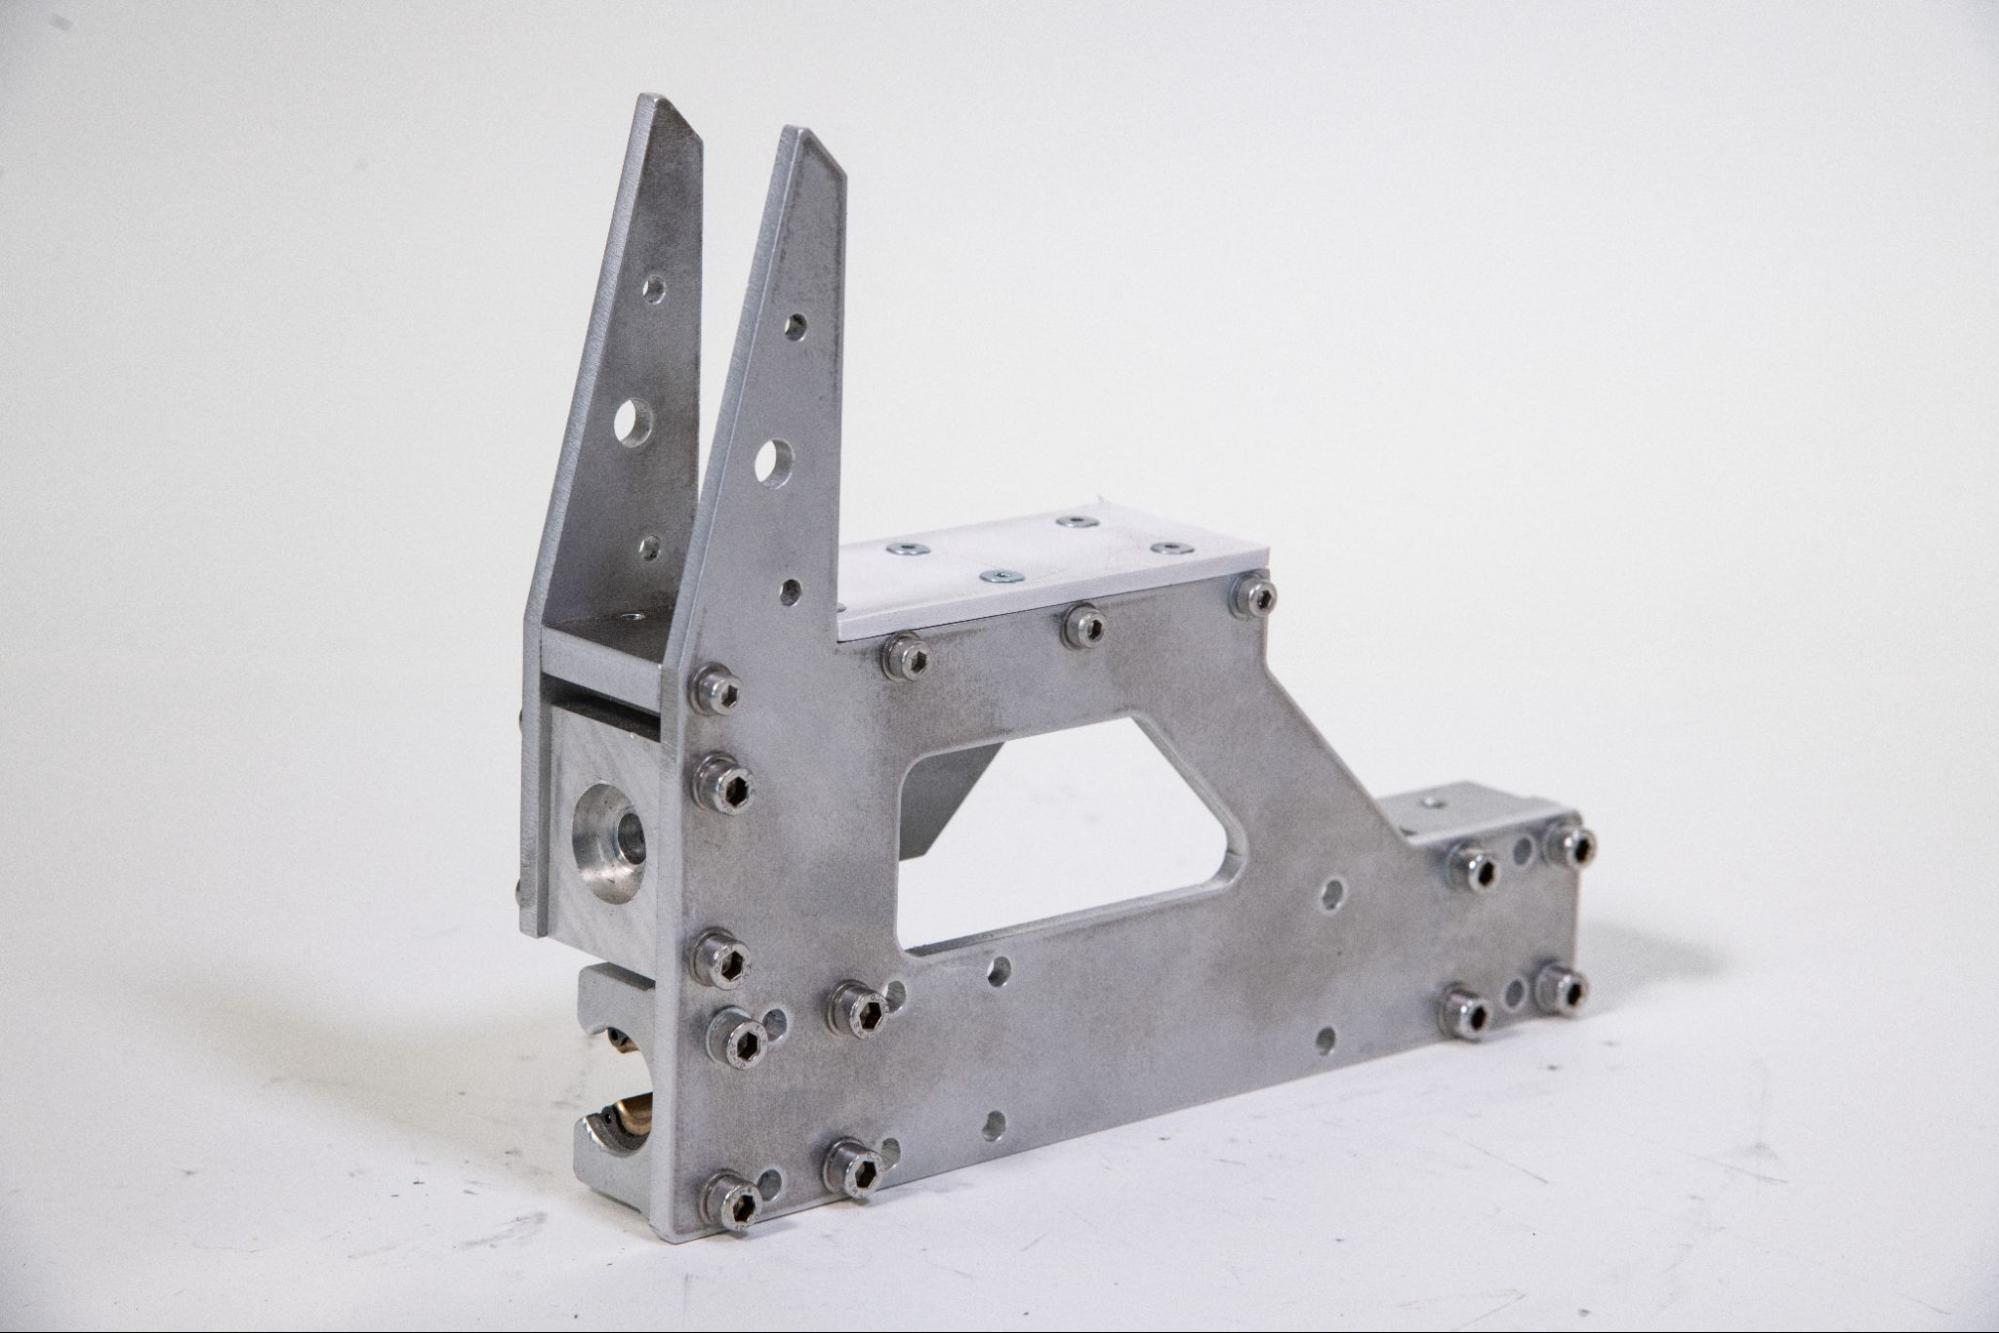
\includegraphics[width=\textwidth]{images/04-3/cl1-jaw-left.jpg}
        % \caption{SubFigureCaption}
        %\label{fig:uniquesubfigurelabel}
    \end{subfigure}
    \hfill
    \begin{subfigure}[b]{0.49\textwidth}
        \centering
        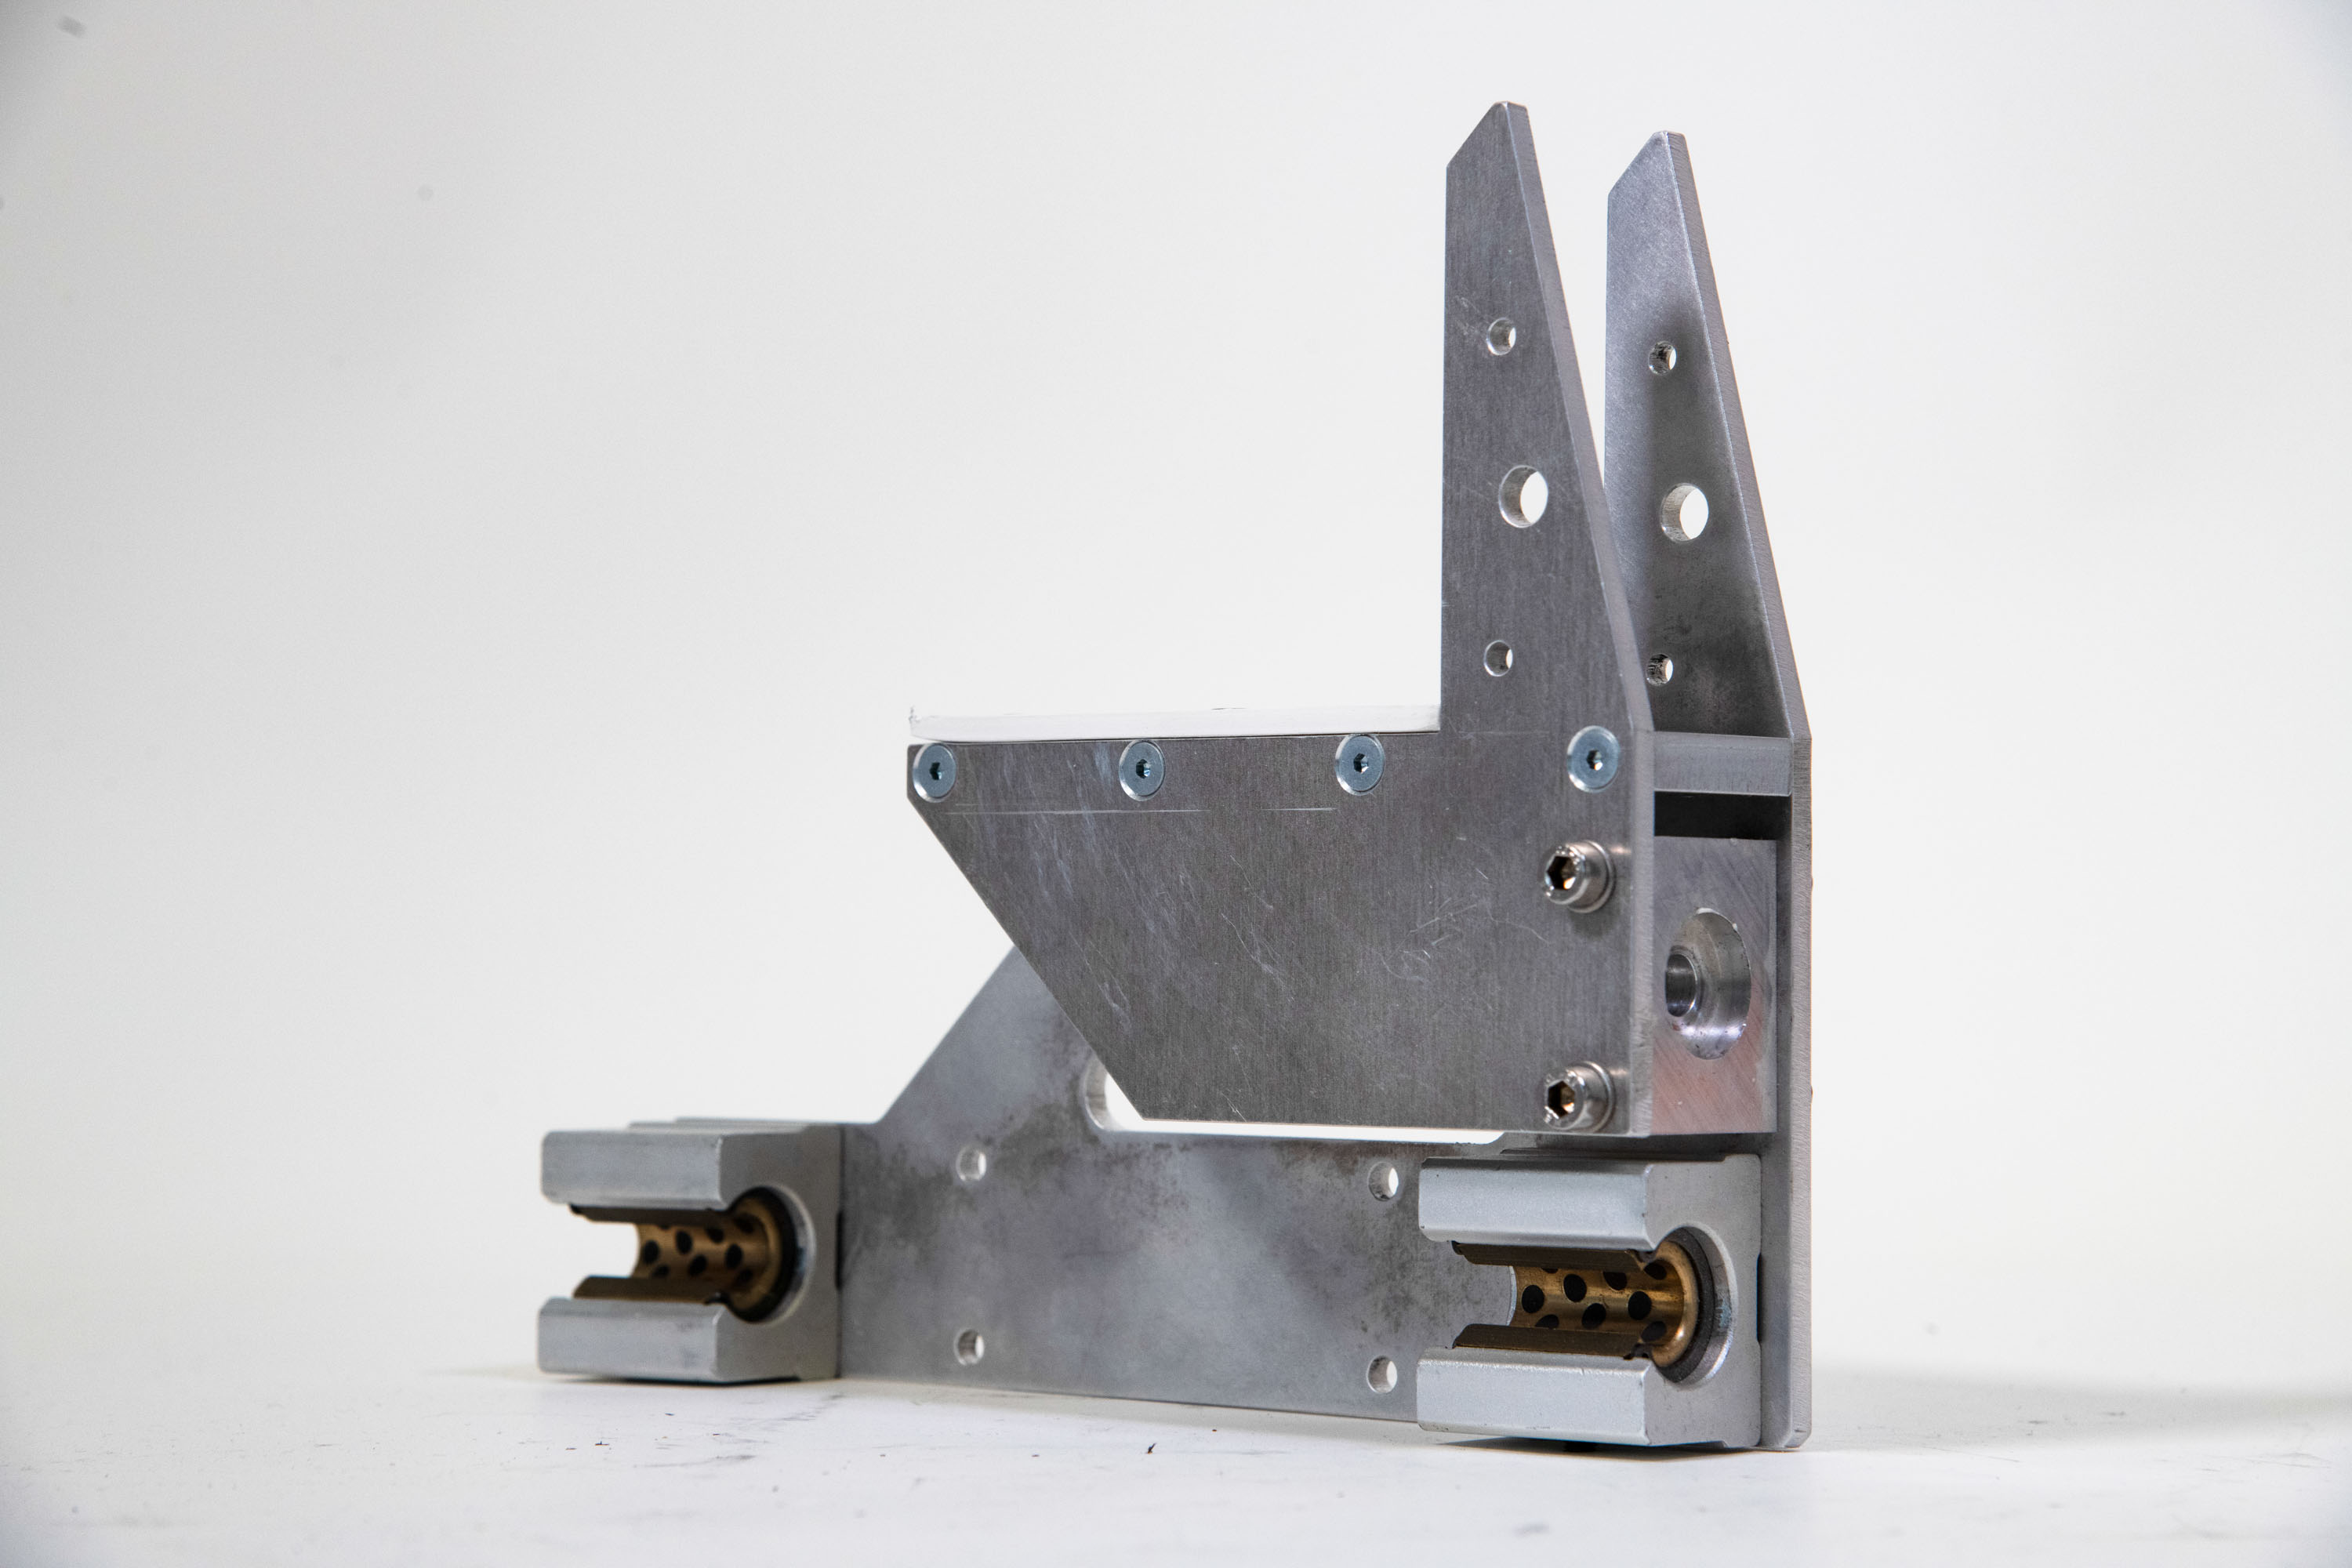
\includegraphics[width=\textwidth]{images/04-3/jaw-right.jpg}
        % \caption{SubFigureCaption}
        %\label{fig:uniquesubfigurelabel}
    \end{subfigure}
    \caption[Photo of the detached clamp jaw from the guide shaft and linear actuator]
    {Photo of the detached clamp jaw from the guide shaft and linear actuator, two bronze bushing is visible on the right image}
    \label{fig:cl1-clamp-jaw}
\end{figure}

\subsubsection{Gripper for Hanging Clamp}
\label{subsubsection:exploration-1-gripper-for-hanging-clamp}

The clamp consists of two symmetrically designed jaws and actuators. They are connected to a common body through a pneumatic parallel gripper. This parallel gripper allows a linear closing motion for the two sides of the clamp jaw to close onto a beam.
The contact surface between the clamp jaw and the timber has a 3D-printed plastic plate with pin features to allow better grappling and secure hanging. A tension spring is used to keep the gripper closed and it can only be opened when the device is docked to the robotic arm and compressed air is provided through the docking adapter. This is intended to be a safety feature, such that the clamp cannot fall on its own due to control error.

Figure \ref{fig:hanging-gripper-test} shows the parallel gripper mechanism and alignment features (the black area) being tested separately from the rest of the clamp. The position of the pins and their geometry were iterated for a few times before settling on this design. The challenge is that the external geometry of the timber beams have a large production tolerance, the location of the drilled holes can also be inaccurate. Therefore, the geometry of the L-shaped pad and the pins must accommodate this error such that the gripper can close completely and maintain a rigid hanging hold afterwards.

\begin{figure}[h!]
    \centering
    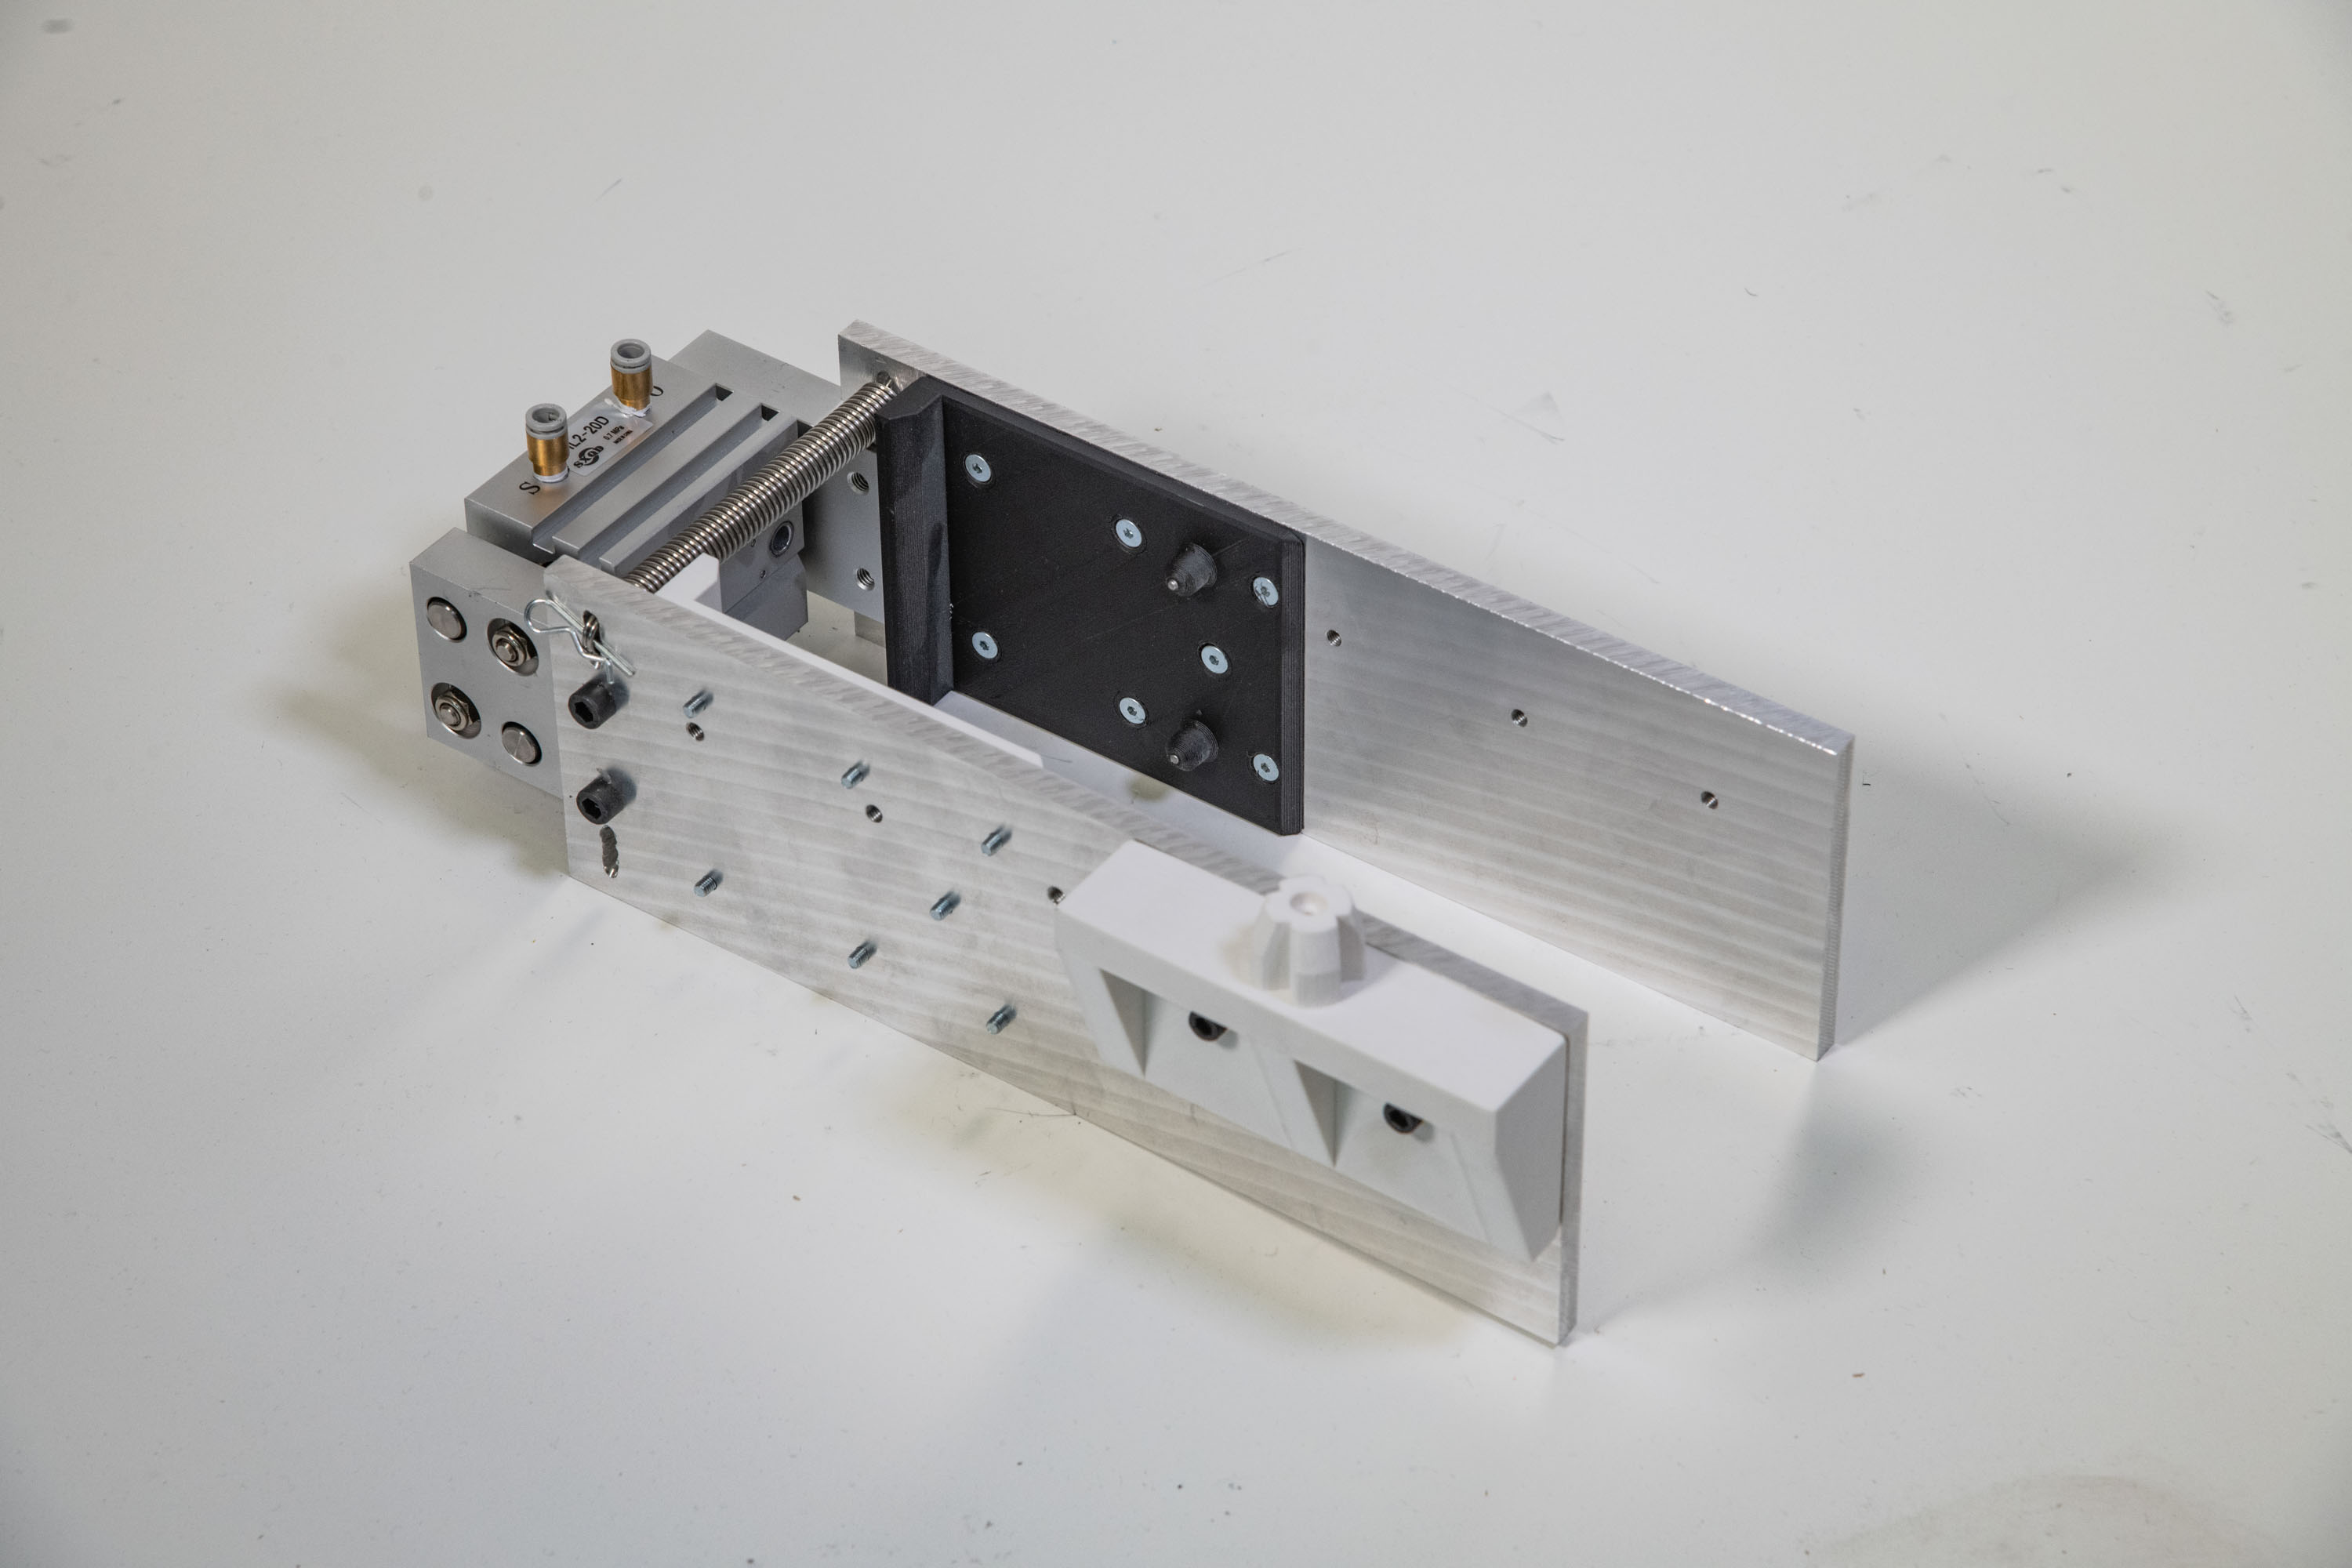
\includegraphics[width=0.99\textwidth]{images/04-3/cl1-hanging-test.jpg}
    \caption{Test setup of hanging gripper and alignment features}
    \label{fig:hanging-gripper-test}
\end{figure}

The registration holes on the beam are intended to be drilled by the automatic joinery machine. However, during this exploration round, they are drilled manually using a precision-made drilling guide (see Figure \ref{fig:drilling-jig}). This guide would be securely clamped around the 100mm x 100mm timber beam before all the necessary holes are drilled. A depth stopper was used to ensure the drilling depth. Different drilling positions can be seen on the guide used during testing and development.

\begin{figure}[h!]
    \centering
    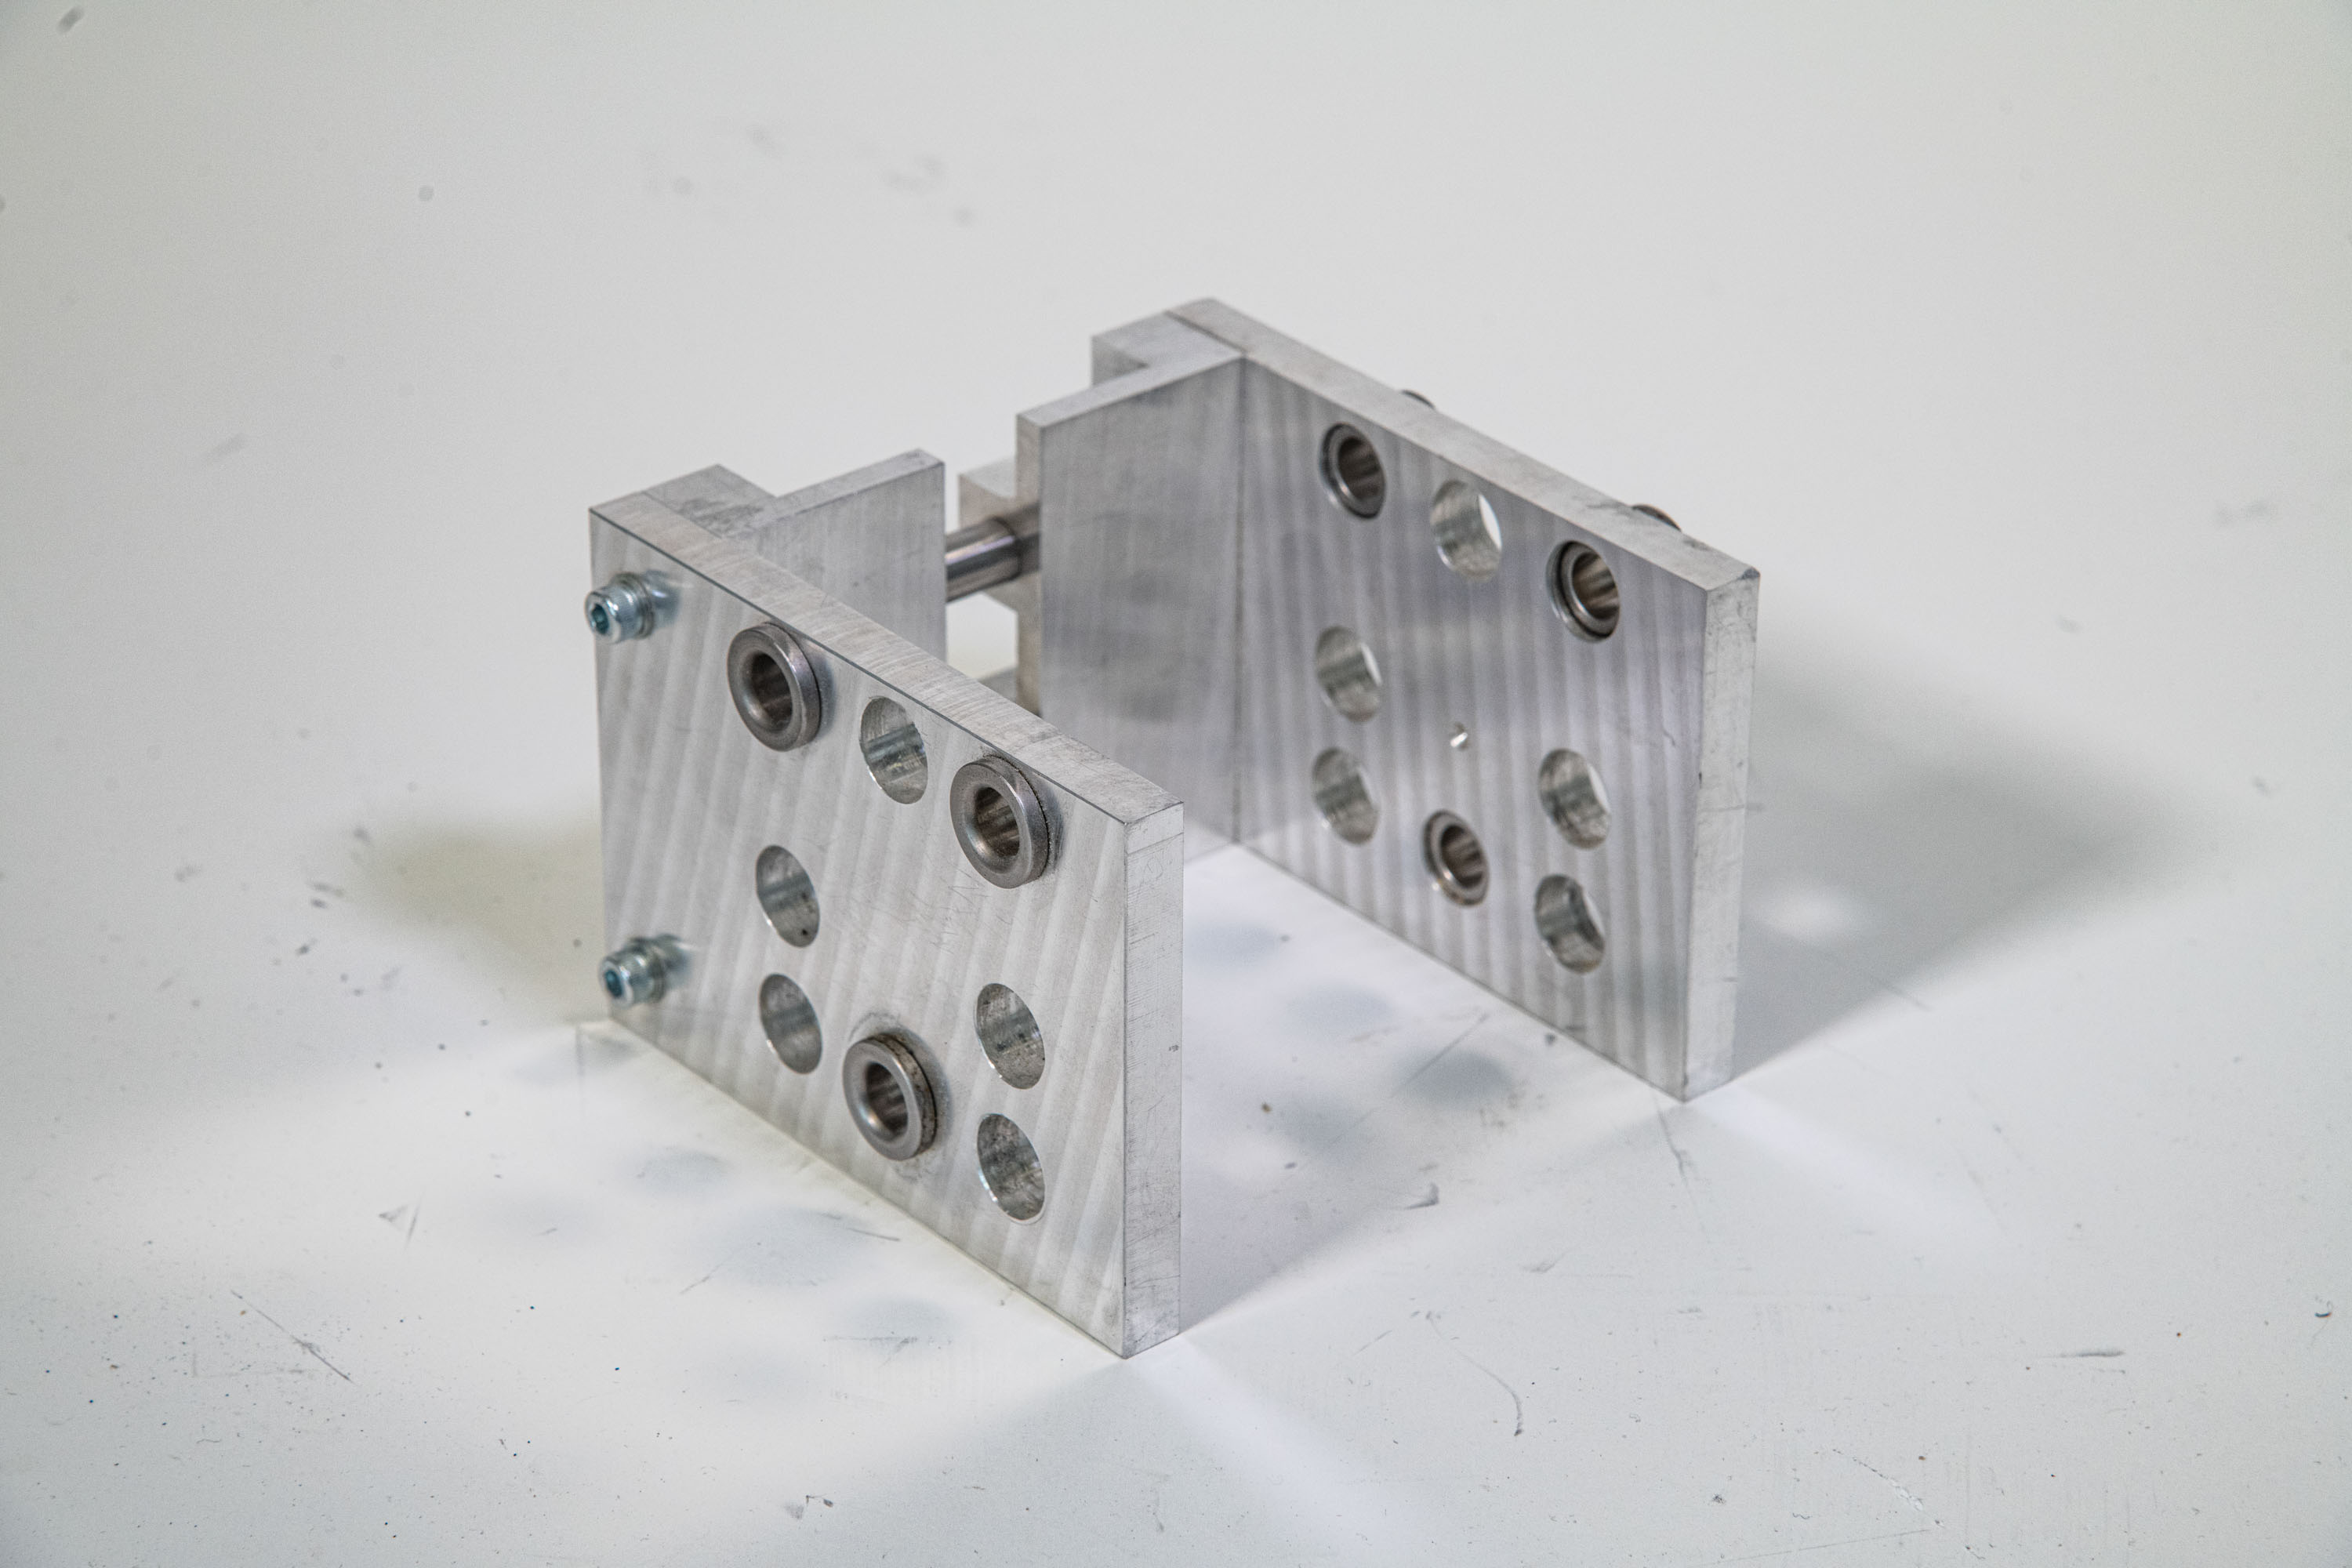
\includegraphics[width=0.99\textwidth]{images/04-3/cl1-pin-drill-jig.jpg}
    \caption{Drilling jig for drilling registration holes on the timber beam}
    \label{fig:drilling-jig}
\end{figure}



\subsubsection{Beam Rest Feature}
\label{subsubsection:exploration-1-beam-rest-feature}

The clamp is designed with a jaw that can be fitted with different plastic inserts for exploring different registration features. The features are intended to assist the alignment between the two beams. Figure \ref{fig:beam-rest-feature} show the initial design of a wedge-shaped alignment feature for guiding the beam in the horizontal direction. However, the plastic insert was never fabricated or tested because the experimental observation \seeref{subsection:exploration-1-beam-support-needed-during-clamping} has already invalidated the resting principle.

\begin{figure}[p]
    \centering
    \begin{subfigure}[b]{0.49\textwidth}
        \centering
        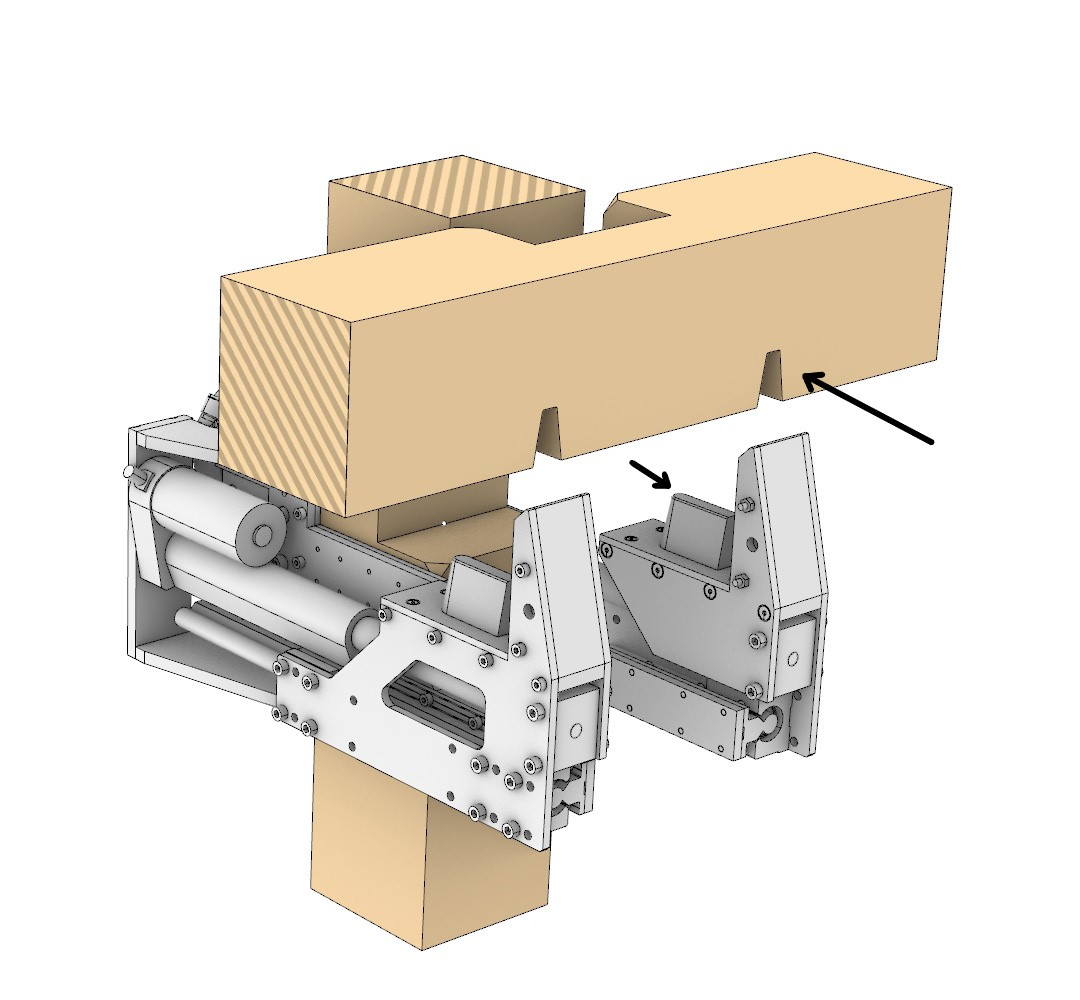
\includegraphics[width=\textwidth]{images/04-3/beam-rest-arrow.jpg}
        \caption{Beam about to be placed in clamp}
        %\label{fig:uniquesubfigurelabel}
    \end{subfigure}
    \hfill
    \begin{subfigure}[b]{0.49\textwidth}
        \centering
        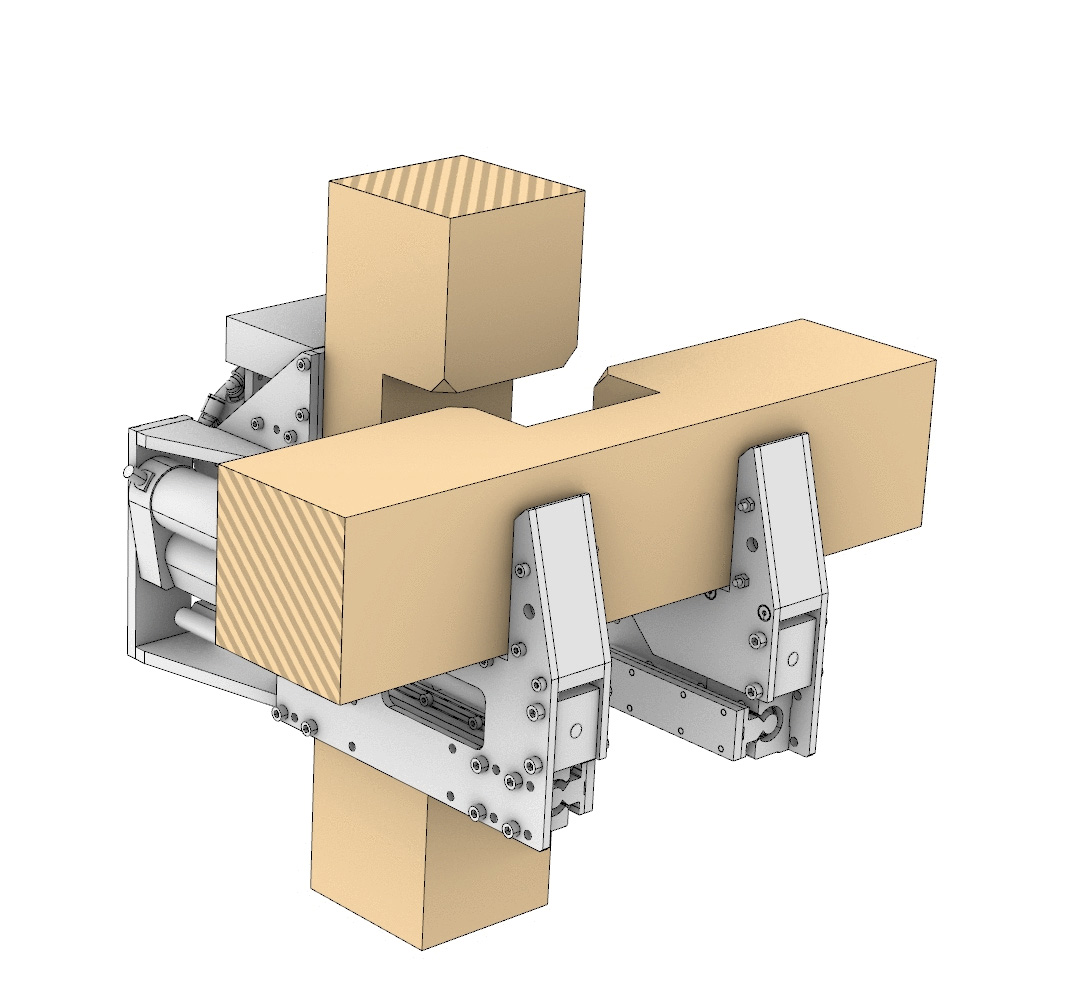
\includegraphics[width=\textwidth]{images/04-3/beam-rest2.jpg}
        \caption{Beam after being placed on the resting feature}
        %\label{fig:uniquesubfigurelabel}
    \end{subfigure}
    \caption{Sketch of a beam rest with wedge-shaped alignment feature} 
    \label{fig:beam-rest-feature}
\end{figure}


\subsubsection{Hardware Integration}
\label{subsubsection:exploration-1-hardware-integration}

The combined design of all the CL1 components can be seen in Figure \ref{fig:integrated-cl1-hardware}. The total weight of the clamp is 4.9kg. There is an intended location for the position of electronics. During the test, it was not installed at that location.

Figure \ref{fig:integrated-cl1-photo} shows the constructed CL1 clamp. Only one is made for the test. The motor cable (black) and the load cell cable (orange) can be seen leading out of the device.

Figure \ref{fig:cl1-attach-to-joint} shows how the clamp is intended to be attached to a lap joint by the robotic arm and then hanging from it. However, this clamp was never docked to the robotic arm during tests.

\begin{figure}
    \centering
    \begin{subfigure}[b]{0.49\textwidth}
        \centering
        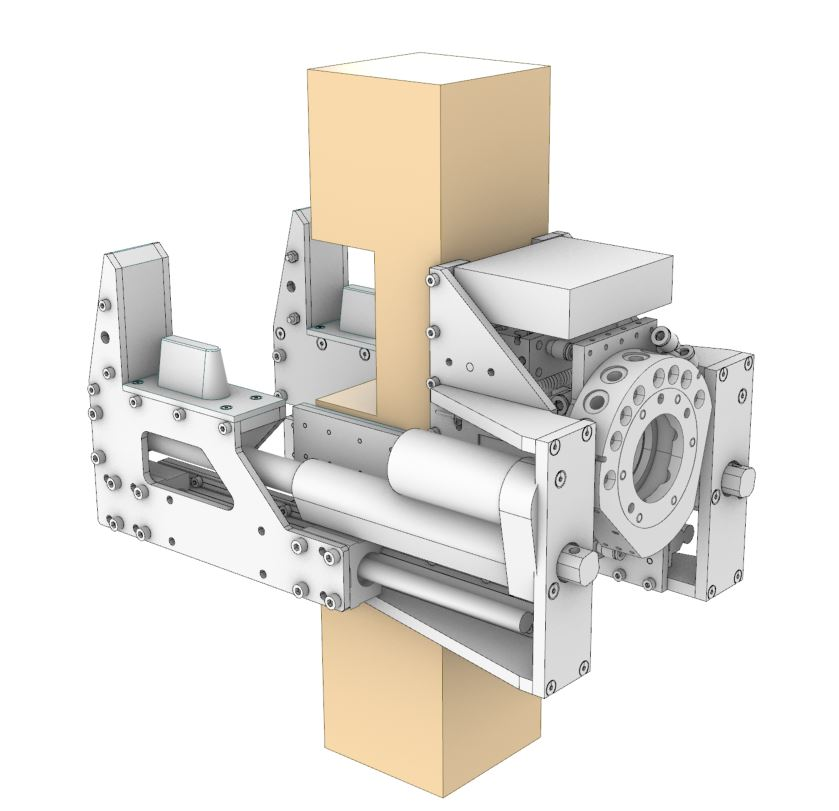
\includegraphics[width=\textwidth]{images/04-3/CL1_back.jpg}
        % \caption{Beam about to be placed in clamp}
        %\label{fig:uniquesubfigurelabel}
    \end{subfigure}
    \hfill
    \begin{subfigure}[b]{0.49\textwidth}
        \centering
        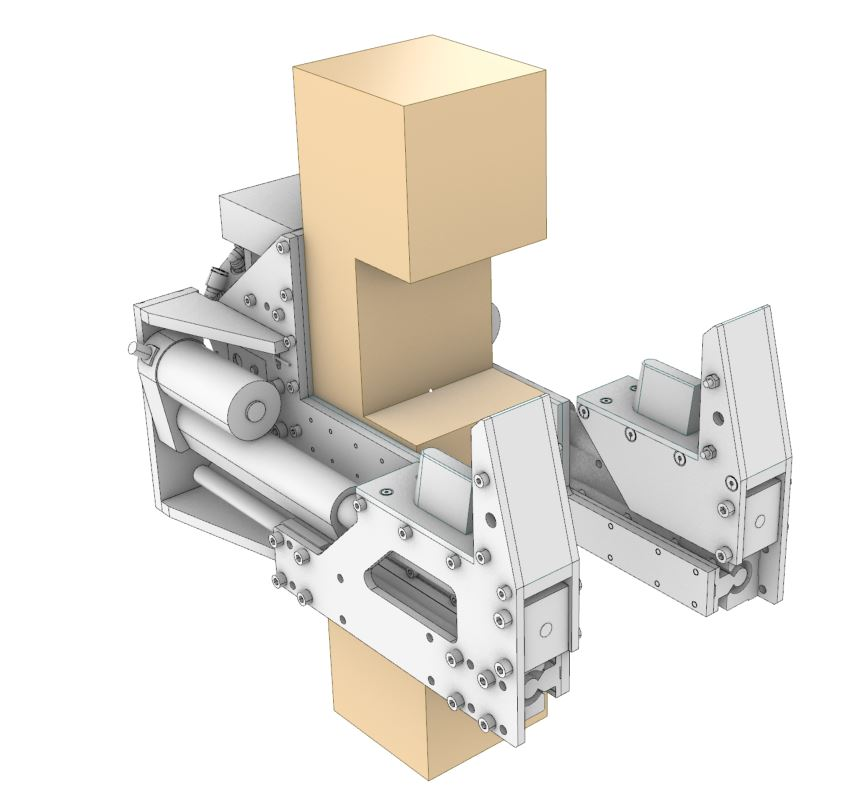
\includegraphics[width=\textwidth]{images/04-3/CL1_front.jpg}
        % \caption{Beam after being placed on the resting feature}
        %\label{fig:uniquesubfigurelabel}
    \end{subfigure}
    \caption{Integrated design of the CL1 clamp} 
    \label{fig:integrated-cl1-hardware}
\end{figure}

\begin{figure}
    \centering
    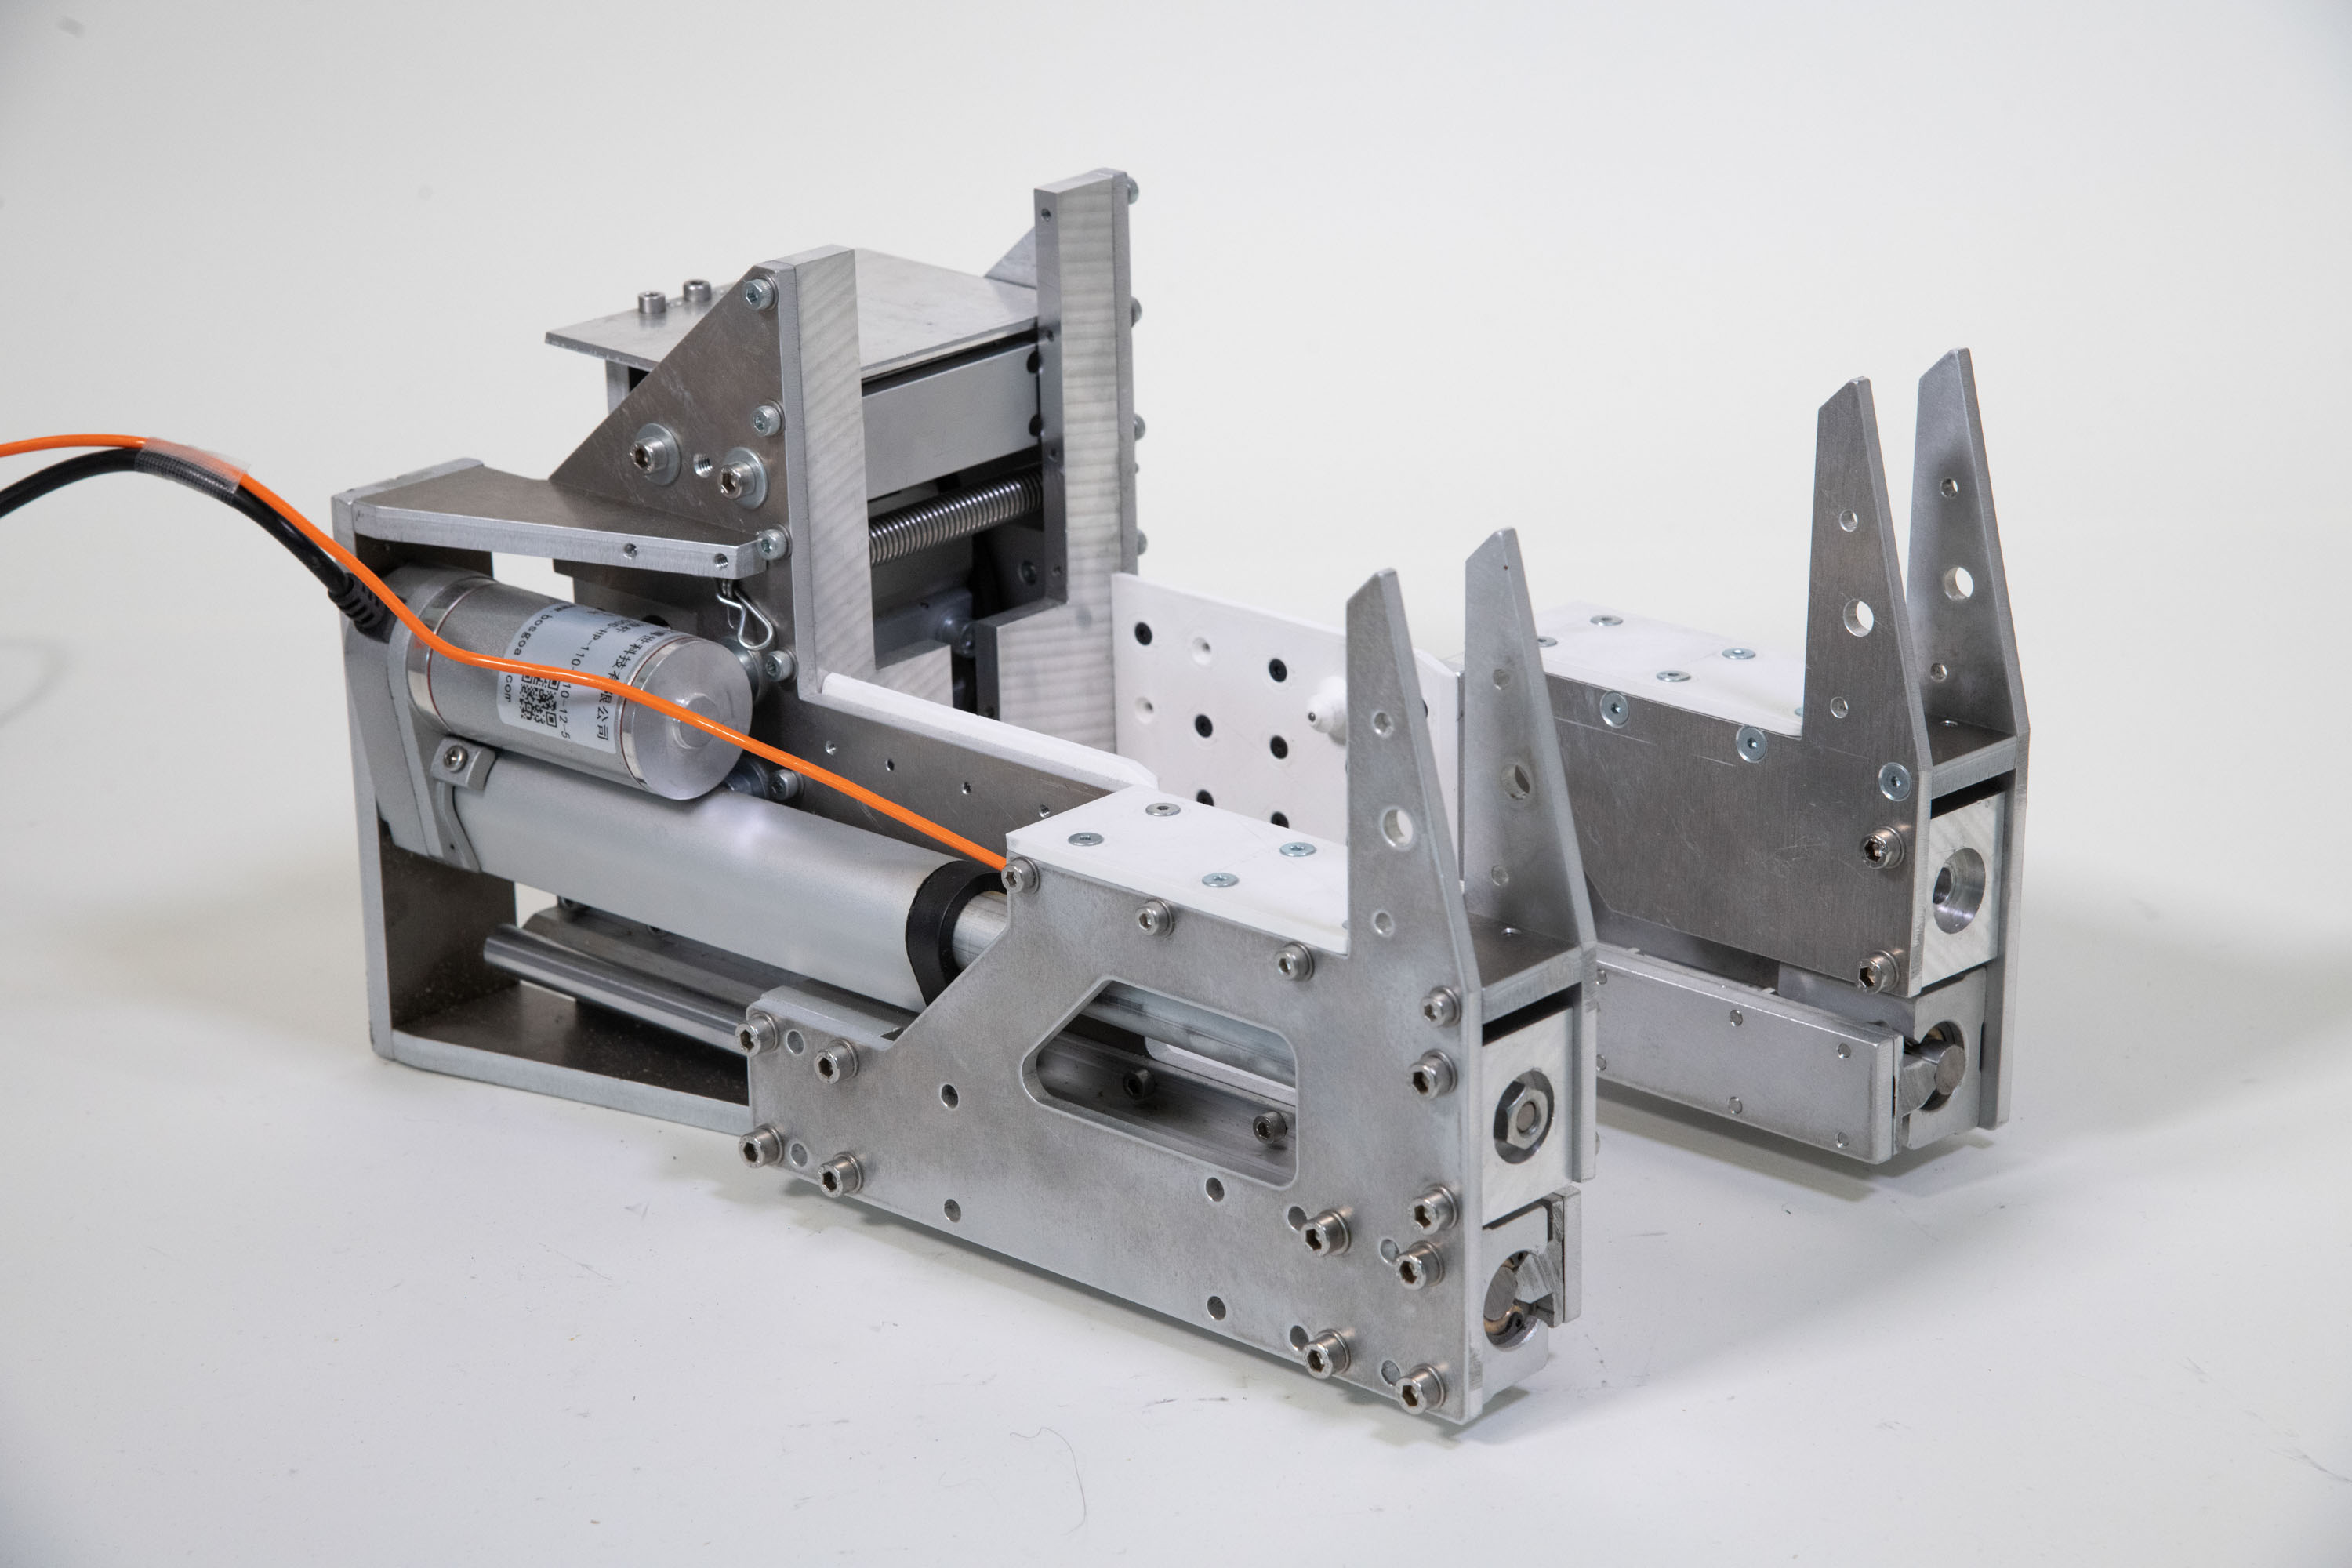
\includegraphics[width=0.99\textwidth]{images/04-3/cl1-completed.jpg}
    \caption{Drilling jig for drilling registration holes on the timber beam}
    \label{fig:integrated-cl1-photo}
\end{figure}

\begin{figure}
    \centering
    \begin{subfigure}[b]{0.90\textwidth}
        \centering
        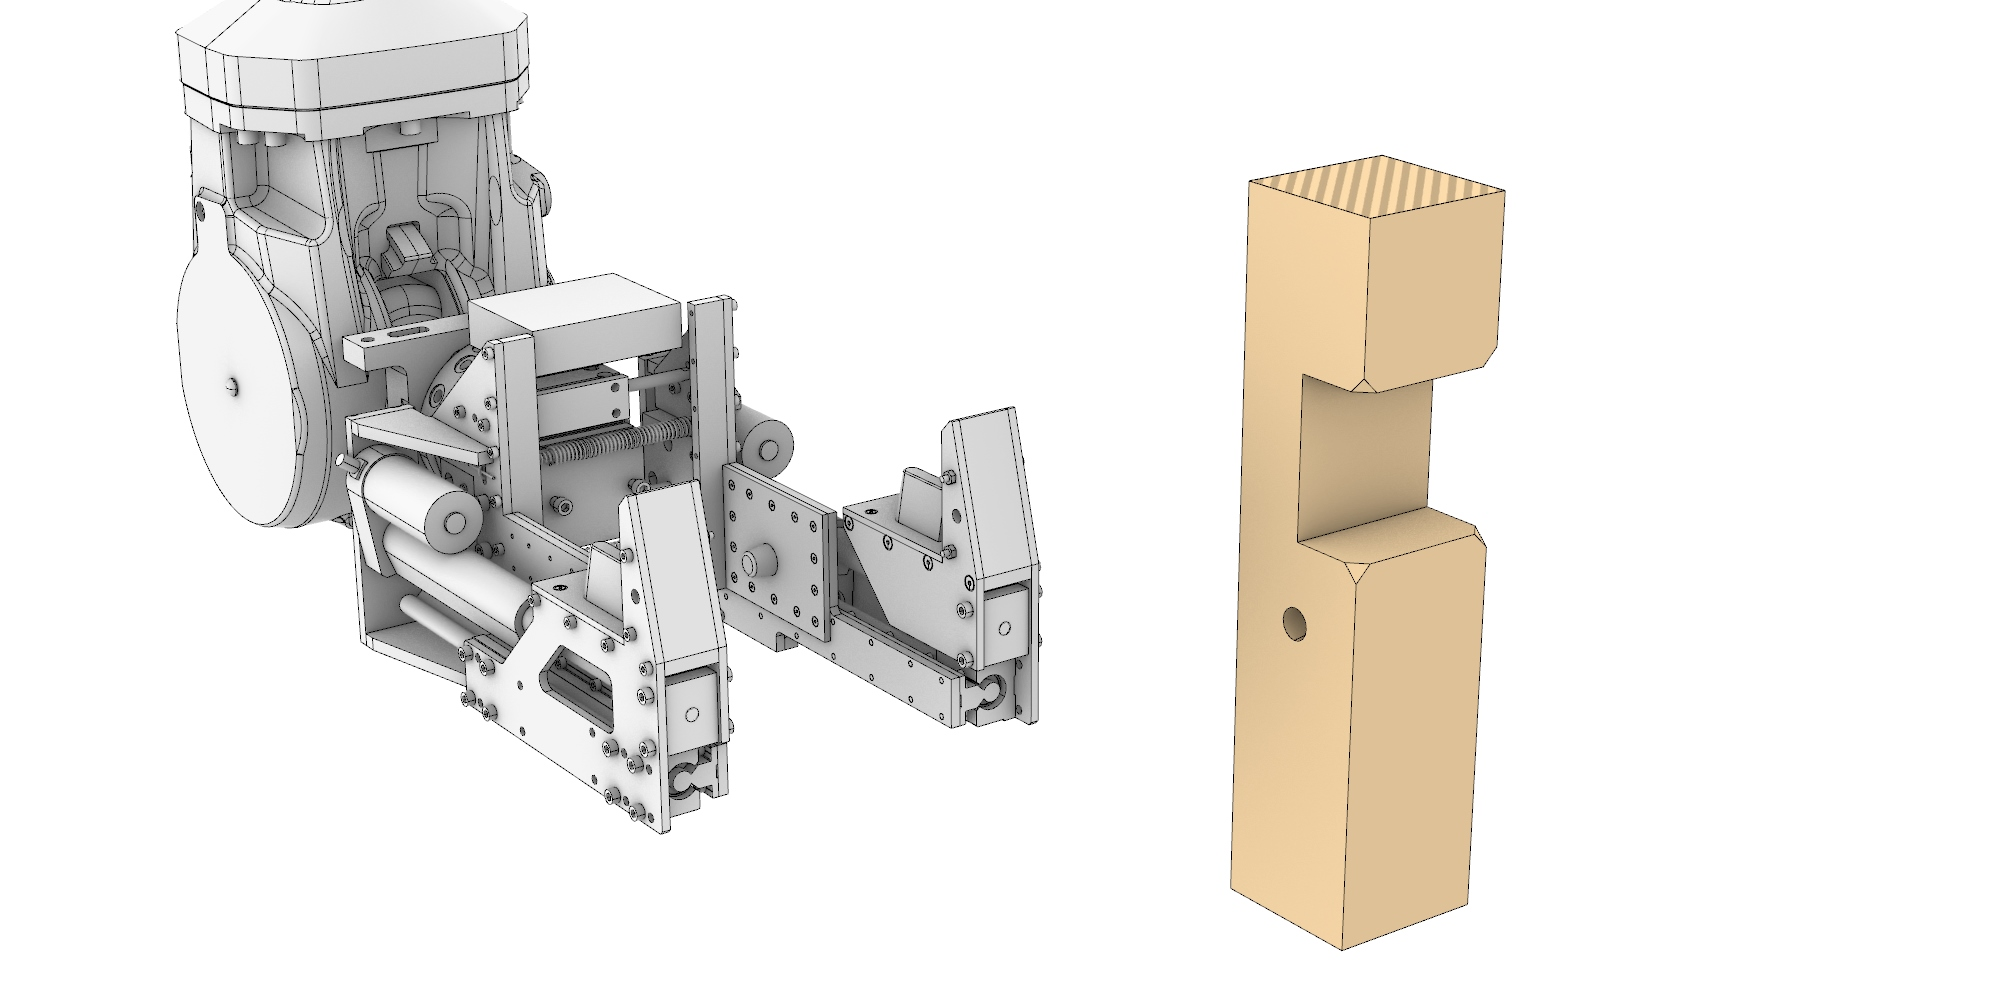
\includegraphics[width=\textwidth]{images/04-3/Attach_1.jpg}
        % \caption{SubFigureCaption}
        %\label{fig:uniquesubfigurelabel}
    \end{subfigure}
    \vskip\baselineskip % Next row

    \begin{subfigure}[b]{0.90\textwidth}
        \centering
        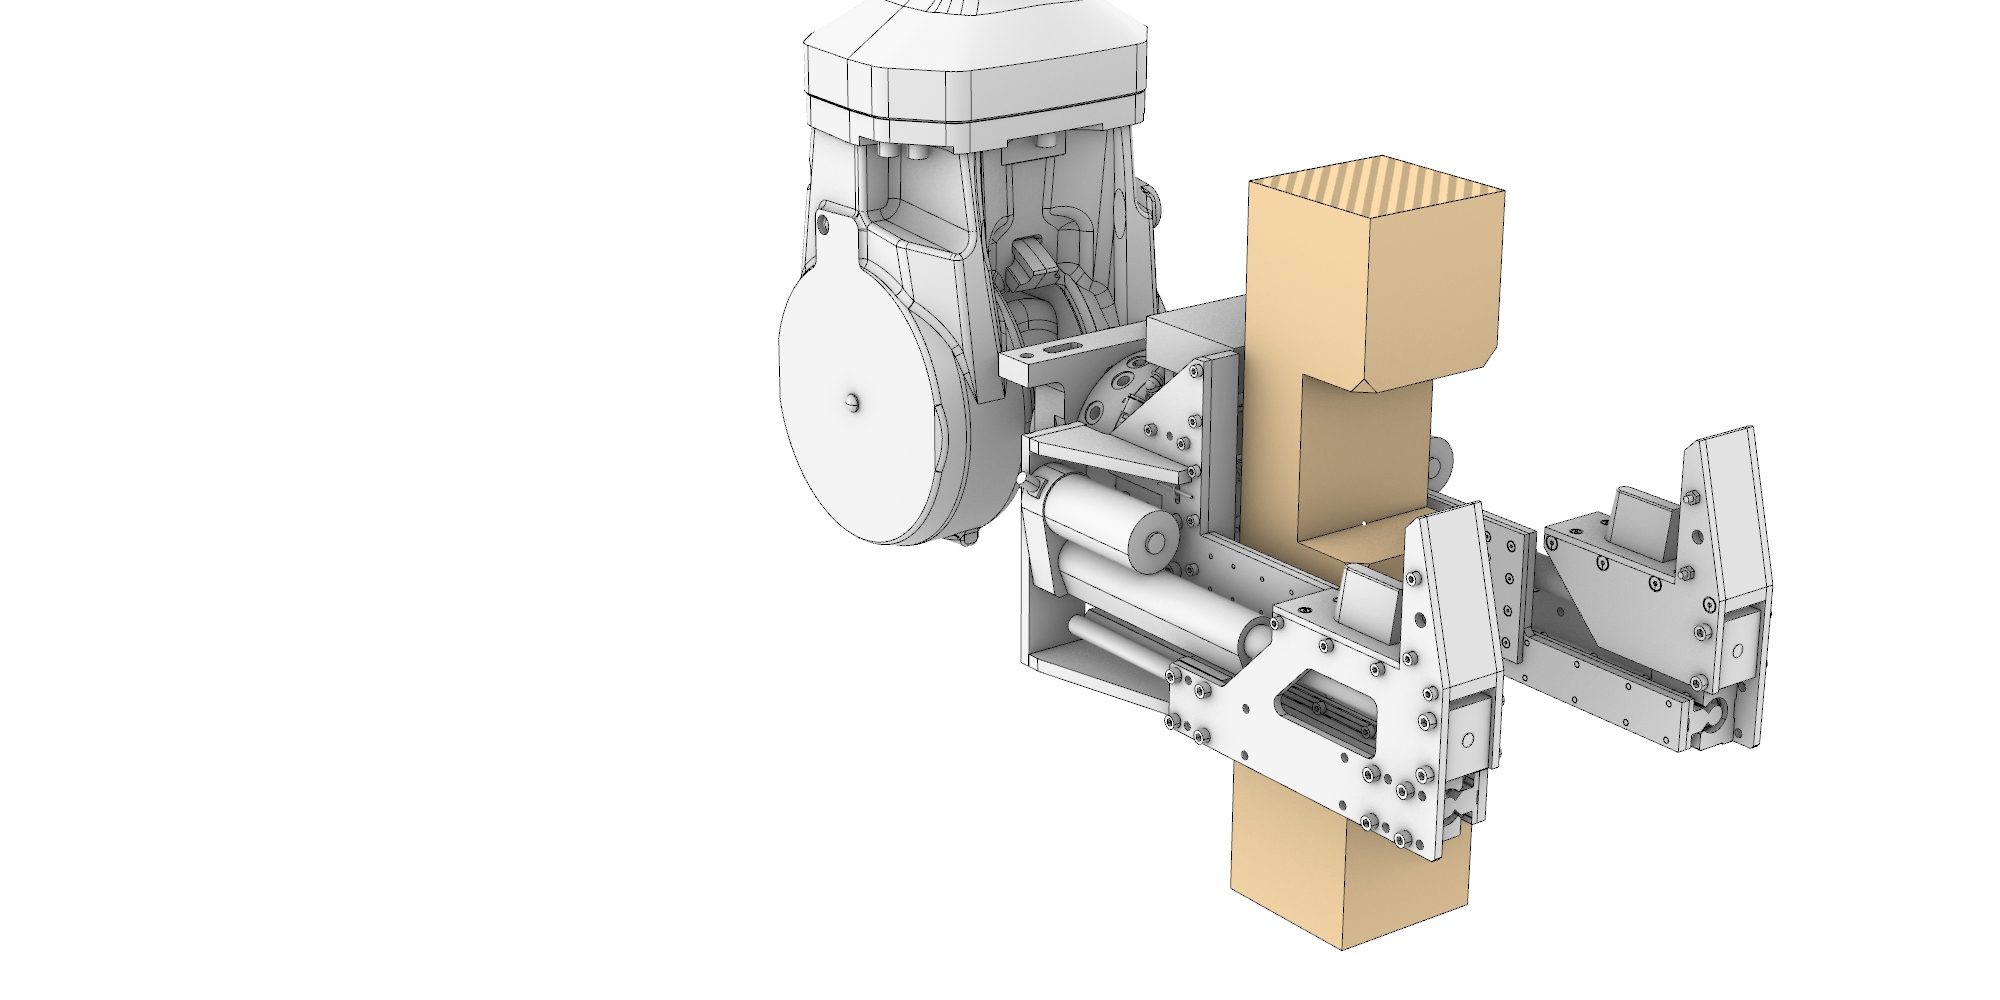
\includegraphics[width=\textwidth]{images/04-3/Attach_7.jpg}
        % \caption{SubFigureCaption}
        %\label{fig:uniquesubfigurelabel}
    \end{subfigure}
    \vskip\baselineskip % Next row

    \begin{subfigure}[b]{0.90\textwidth}
        \centering
        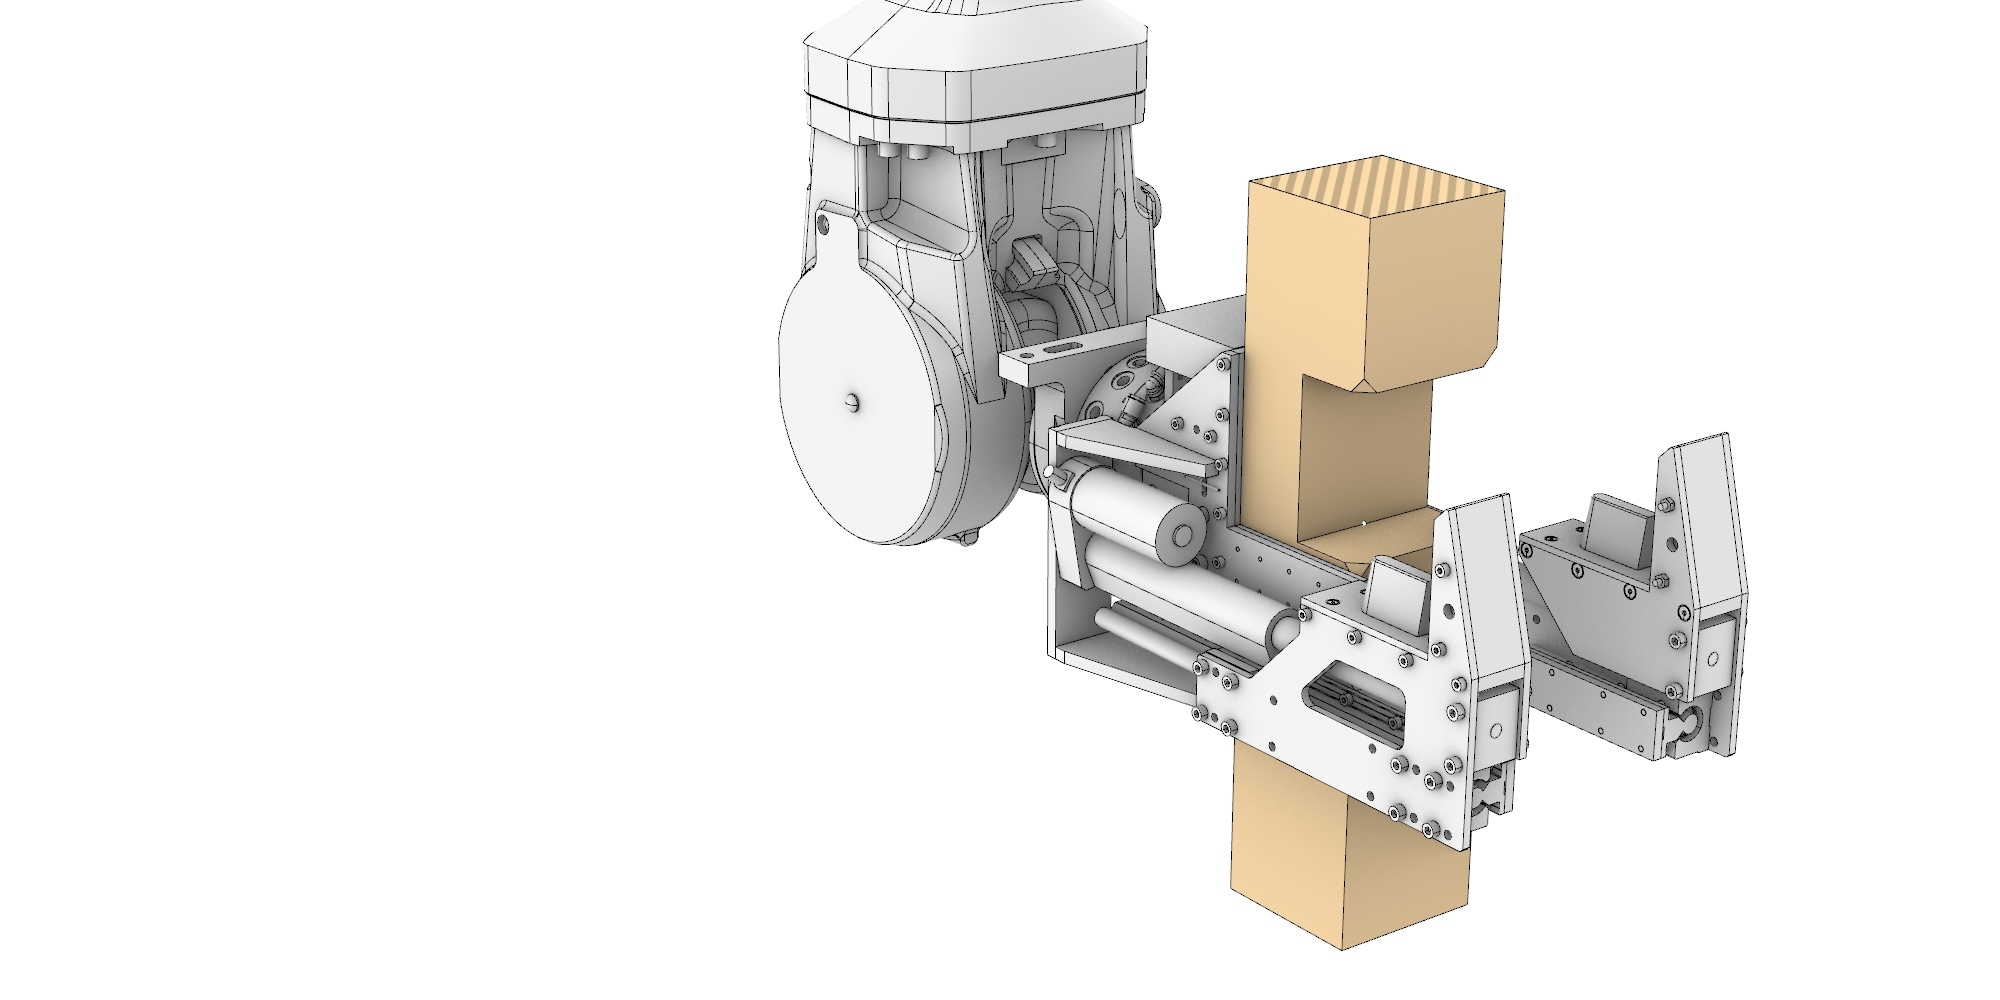
\includegraphics[width=\textwidth]{images/04-3/Attach_11.jpg}
        % \caption{SubFigureCaption}
        %\label{fig:uniquesubfigurelabel}
    \end{subfigure}

    \caption{Diagram sequence showing how the clamp is attached to a lap joint}
    \label{fig:cl1-attach-to-joint}
\end{figure}

\subsection{CL1 Clamp Drive System}
\label{subsection:exploration-1-cl1-clamp-electronics}

Being the first DiRT electronic controller, the CL1 Clamp controller was designed together with the creation of the motor control algorithms, which had a large influence on the choice of components. The initial goal of the electronics development is to identify a combination of control algorithms, choice of motor, encoder, and motor driver that allows controlled movement of the two motors following a predefined trajectory.
After the initial goal is successful, the setup is also added with other features as part of a validation test to confirm major systems:

\begin{itemize}[nosep]
    \item LiPo battery power input for motor driver
    \item Regulation of battery voltage for controller logic voltage
    \item Wireless communication using radio module
\end{itemize}

\subsubsection{System Voltage}
\label{subsubsection:exploration-1-system-voltage}

The development started by identifying the system voltage, which depended on the choice of battery and actuator motor. In order to maximise the power available in short-burst output, I decided the best battery chemistry choice is Lithium Polymer (LiPo) because of its high power density. Table \ref{table:common-lipo-properties} listed some of LiPo properties at the time of writing:

\begin{table}[]
    \includegraphics[page=3, trim=25.4mm 210mm 25.4mm 33mm, clip, width=\textwidth]{tables/Tables in Chapter 4.pdf}
    \caption{Common lithium polymer battery properties}
    \label{table:common-lipo-properties}
\end{table}

Considering that most of the common DC motors are either 12V or 24V, I decided the best motor and battery combination would be a 12V motor with a 4S battery. The battery voltage can range between 12.8V (discharged) and 16.8V (fully charged), which leaves some margin for voltage drop during operation and can be throttled by PWM control over the driver if necessary. The selected linear actuator also runs on 12V \seeref{subsubsection:exploration-1-linear-actuator-and-jaw-design}.

\subsubsection{Motor Driver}
\label{subsubsection:exploration-1-motor-driver}

The choice of motor driver is a Dual H-Bridge Motor Controller (XY160D manufactured by Handson Technology) (See Table \ref{table:hbridge-xz160d-properties} for its specifications) which weighted only 32 grams. The H-Bridge configuration allows bi-directional DC motor control that is necessary for clamp jaw retraction and extension. This type of H-Bridge motor driver is very common and is made by many different companies with different current ratings. The intention of choosing this type of driver is to facilitate future upgrades if necessary. 

\begin{table}[]
    \includegraphics[page=4, trim=25.4mm 210mm 25.4mm 33mm, clip, width=\textwidth]{tables/Tables in Chapter 4.pdf}
    \caption{Properties of the Dual H-Bridge Motor Controller XY160D}
    \label{table:hbridge-xz160d-properties}
\end{table}

The motor driver supports four possible control modes (see Table \ref{table:hbridge-xz160d-control-logic}). Its control logic is a common scheme that is made famous by the L298 motor driver chip and is commonly found on motor drivers. There are three digital signal inputs, IN1, IN2, and ENA. ENA represents motor enable, which can be supplied with a PWM signal to throttle the motor.

\begin{table}[]
    \includegraphics[page=5, trim=25.4mm 210mm 25.4mm 33mm, clip, width=\textwidth]{tables/Tables in Chapter 4.pdf}
    \caption{Control logic of Motor Controller XY160D}
    \label{table:hbridge-xz160d-control-logic}
\end{table}

\subsubsection{LiPo Battery}
\label{subsubsection:exploration-1-lipo-battery}

Based on the specification of the chosen linear actuator, the 12V option is rated at 60W with 5mm/s at 2000N output. It will draw 5A at constant maximum power, which should be compatible with this 7A driver. It will take approximately 20 seconds to traverse 120mm, assuming 80\% driver efficiency, each full stroke which will consume about 35mAh. A complete cycle of clamping and retraction can consume roughly 70mAh. Based on this rough calculation, a 1000mAh battery was chosen, as it will support approximately 10 cycles, assuming the battery has only 80\%-90\% usable capacity.   
Table \ref{table:lipo-battery-survey} listed some of the 4S LiPo batteries on the market as of April 2023. 

\begin{table}[]
    \includegraphics[page=6, trim=25.4mm 210mm 25.4mm 33mm, clip, width=\textwidth]{tables/Tables in Chapter 4.pdf}
    \caption{Survey of 4S LiPo batteries on the market}
    \label{table:lipo-battery-survey}
\end{table}

Different capacities were tested with no major performance difference being observed, the only difference is that larger capacity would provide more operation cycles between recharge.

\subsubsection{Microcontroller}
\label{subsubsection:exploration-1-microcontroller}

The Arduino family of microcontroller boards was selected for this development due to their extensive library support for integrated and external hardware. 
\textbf{Arduino Uno} was chosen for initial tests development, the reason being:

\begin{itemize}[nosep]
    \item Low cost and widespread availability.
    \item Presence of two external interrupt signal inputs, making it suitable for counting motor encoder output. 
    \item Integrated USB serial communication, which greatly simplifies debugging and control.
    \item Equipped with an ATmega328 CPU running at 16 MHz, these Arduino boards are popular choices for embedded motion control tasks.
\end{itemize}

The Arduino Uno is later switched to \textbf{Arduino Nano}, which has the same functionality but a smaller form factor. The following General Purpose Input Output (GPIO) pins are used:

\begin{itemize}[nosep]
    \item The motor drivers require three digital signals, one of which requires PWM output, for controlling each motor channel. The two channels occupied 6 pins. 
    \item There are two encoder channels from each motor, one of which is connected to the external interrupt pin. In total, both motor encoders occupied 4 pins.
    \item There are provisions for connecting to the CC1101 radio module and two load cells. This was tested during development but was not implemented for the demonstration. The integration with the radio module is continued in the next Exploration Round.
    \item One of the Analog-to-Digital Converter (ADC) input pins is used for monitoring battery voltage.
\end{itemize}

In order to monitor battery voltage, it is connected to the ADC over a voltage divider with a ratio of 3.35 to 1 (see the schematic below). A fully charged LiPo 4S battery at 16.8V will be reduced to 5.01V, which coincides with the upper bound of the ADC. The ADC has 10 bit resolution (1024 steps) or 0.00488V per step \\($5.0V / 1024 steps$). This circuit design will provide an effective resolution ($R_{Eff}$) between a full battery at 16.8V and an empty battery at 12.8V : 
\\ $R_{Eff} = (16.8V - 12.8V) / 0.00488V = 243 steps$

The \textit{Measured Voltage} is related to the \textit{Raw Values} (obtained from the ADC) by a divisor variable and an offset variable. Values of which has to be calibrated after construction for each device to compensate for component deviations. 

\paragraph{Validation}

The Motor Driver and the Arduino Uno were validated in a test setup before the development of the schematics. The test confirmed:
\begin{itemize}
    \item Bi-direction control of the actuator using the driver
    \item Encoder output can be read using the interrupt pins
    \item Motion and driver operation under 12V power, without PWM throttle
\end{itemize}

\subsubsection{Voltage Regulation}
\label{subsubsection:exploration-1-voltage-regulation}

During remote-controlled operation, the 16.8V battery power had to be regulated to 5V for the Arduino microcontroller. A simple linear regulation circuitry based on LM7805 was used for the regulation. Due to the large voltage drop (11.8V), the efficiency of the regulation was expected to be low. However, the low current drawn from the microcontroller (19 mA) and the encoders (4 mA) should not create a power and heat dissipation problem.

The following calculation was performed using ambient temperature $T_A = 25^{\circ}C$. The thermal resistance of the TO-220 package $\theta_{JA} = 19^{\circ}C/W$. Without a heatsink, the package-to-ambient is approximately $70 ^{\circ}C/W$.

Power Dissipation $P_D = (V_{in} - V_{out}) * I_{out} = (11.8V) \times 23mA = 271mW$

Using the thermal formula obtained from LM7805 spec sheet, the junction temperature of the chip $T_J$ can be computed. The result is that the junction temperature is far below the maximum junction temperature $T_J{max} = 150^{\circ}C$.

\begin{align}
    P_D &= (T_J - T_A) / \theta_{JA}\nonumber \\
    0.271W &= (T_J - 25^{\circ}C) / (19^{\circ}C/W + 70^{\circ}C/W)\nonumber \\
    T_J &= 49.1^{\circ}C\nonumber
\end{align}

\subsubsection{Schematics}
\label{subsubsection:exploration-1-schematics}

The schematic of the controller is shown in Figure \ref{fig:schematic-cl1-controller}, including the assignment of pins on the Arduino controller.

\begin{figure}
    \centering
    \includegraphics[width=0.90\textwidth]{images/04-3/SerialController_Schematic.png}
    \caption{Schematic of the CL1 Clamp Controller}
    \label{fig:schematic-cl1-controller}
\end{figure}


\subsubsection{Construction}
\label{subsubsection:exploration-1-construction}

Only one copy of this design was constructed for the test (see Figure \ref{fig:photo-cl1-controller}). It was soldered on a 50mm x 70mm protoboard with a female pin header connector for stacking it above the motor driver module (red). All connections were wired manually with small wires. The four wires with green plugs were intended for connecting to a future wireless communication module. However, it was never tested.

\begin{figure}
    \centering
    \includegraphics[width=0.90\textwidth]{images/04-3/controller-Photo-NoRadio.jpg}
    \caption{Photo of the CL1 Clamp Controller}
    \label{fig:photo-cl1-controller}
\end{figure}

\FloatBarrier

\subsection{CL1 Clamp Firmware}
\label{subsection:exploration-1-cl1-firmware}

The CL1 Clamp Firmware is an Arduino-based motor controller system written in C++ that can control two linear actuators and accepts serial communication for command and control. The main control loop implements non-preemptive scheduling for sharing time between three subroutines. All three subroutines are visited sequentially in each cycle and are allowed to run until it yields control (see Figure \ref{fig:firmware-motion-control-timeshare}). If needed, each subroutine can implement its own timer to determine how frequently it should be executed.\footnote{This feature was used only in later development when there are more subroutines.}.

\begin{enumerate}
    \item \textbf{Read and Process Serial Command} \\ Process command received from USB serial interface. This is intended for debugging as the controller was not yet integrated with wireless communication. \seeref{subsubsection:exploration-1-control-commands}
    \item \textbf{Motor Motion Control} \\ Only active when there is an active motion target. A separate timer is used to fix the motion control frequency. \seeref{subsubsection:exploration-1-bang-bang-motion-control}
    \item \textbf{Battery Monitor}\\ Check battery level using integrated ADC in microcontroller. \seeref{subsubsection:exploration-1-microcontroller}
\end{enumerate}

\begin{figure}[h]
    \centering
    \vskip 20pt
    \includegraphics[width=0.60\textwidth]{images/04-3/cl1-firmware-mainloop.pdf}
    \caption{Diagram showing time sharing between subroutines in the main control}
    \label{fig:firmware-motion-control-timeshare}
\end{figure}

\FloatBarrier

\subsubsection{Control Commands}
\label{subsubsection:exploration-1-control-commands}

The CL1 Clamp Firmware was designed to receive serial commands from the integrated USB serial adapter and provide responses when necessary. Since the USB messaging protocol is completely transparent to the Arduino microcontroller, the serial interface is purely a stream of bytes transmitting at 115200 baud. Command messages are terminated by a '\textbackslash n' character and without start-of-message header. The Command Processing Subroutine monitors the receive buffer and triggers a response when a command is received.

\begin{table}[thb]
    \includegraphics[page=8, trim=25.4mm 130mm 25.4mm 33mm, clip, width=\textwidth]{tables/Tables in Chapter 4.pdf}
    \caption{Commands supported by the CL1 Clamp Firmware}
    \label{table:command-list-cl1-firmware}
\end{table}


All commands received by the firmware are treated as real-time commands, allowing motion to be started, modified, or stopped at any time. This is crucial for upper-level controllers (on a PC) to assert full control over the hardware behaviour and stop it in emergency situations. This behaviour is inspired by many embedded real-time Computer Numeric Control (CNC) motion controllers, such as tinyg2 \parencite{G2core2023} and grbl \parencite{jeonGrbl2019}. 
Table \ref{table:command-list-cl1-firmware} lists all the commands supported by the controller.


In order to avoid blocking the main control loop, all motion commands are processed in an asynchronous manner. This was achieved by setting an internal state in the controller, such as a target position, and defer the execution to the motion control subroutine in the main control loop. The Motion Control Subroutine can then be executed regularly to perform motion control \seeref{section:exploration-1-demonstration}. For other commands, such as the settings \verb|(\$)| commands, the status report \verb|(?)| and the stop command, were executed immediately. 

In this exploration round, there was no mechanism to ensure command packages are not lost during transmission. There was a risk that a movement command may be lost and the controller will not start the motion. This was a known issue that was addressed in the next exploration round \seeref{subsection:exploration-2-clamp-controller-l2}.

\FloatBarrier

\subsubsection{Bang Bang Motion Control}
\label{subsubsection:exploration-1-bang-bang-motion-control}



A linear profile motion controller was implemented to control the motion of the two motors based on encoder readings \parencite{tanPrecisionMotionControl2001}. The motion profile is defined by the following parameters:

\begin{itemize} [nosep]
    \item Velocity - Extracted from \verb|\$0| setting
    \item Start position - Current motor position when the motion command is received
    \item Target position - Target value defined in the motion command
    \item Start time - The time when the motion command is received
\end{itemize}

\begin{figure}[h]
    \centering
    \includegraphics[width=0.99\textwidth]{images/04-3/firmware-motion-control.pdf}
    \caption{Linear motion profile of the CL1 Clamp Firmware}
    \label{fig:linear-motion-profile}
\end{figure}

When the Motor Control Subroutine is entered, it computes the current tracking position using the motion trajectory and computes the {\tt tracking\_position\_error} by comparing it with the encoder readings. 
Figure \ref{fig:linear-motion-profile} shows the motion profile in a graphical way. Green arrows are the parameters that define the motion profile and brown arrows are the changing tracking targets.
The equations of motion are as follows:

\begin{align*}
    delta\_time &= current\_time - motion\_starting\_time \nonumber \\
tracking\_position &= delta\_time \times velocity +  starting\_position \nonumber \\
tracking\_position\_error &= tracking\_position - current\_position \nonumber \\
\end{align*}

A bang-bang control logic is implemented for simplicity. When the position error is positive, the motor is set at full power to catch-up. Otherwise, the motor is set to cruising mode (no power, high impedance) and allowed to slow down. No control deadband was programmed. This low level control subroutine is not being throttled by a timer. Therefore it runs as frequently as the main control loop and therefore it may be executed irregularly. Despite the simplicity of bang-bang control, it was tested to be functional over a variety of speed from 0 to 2mm/s. The mechanical dampening likely contributed to its relatively smooth motion.

During the motion tracking, if the position error is too large, the controller will consider it as a tracking failure and will switch over to a stopped state. This is a protection for when the assembly resistance is too great for the motor to keep up with the designated speed. It is possible to try a failed motion again with a slower speed, but tests have shown that the assembly resistance will eventually increase to the point that the motor cannot keep up again. In general this is referred to as a stall state. 

Extra protection was added to avoid overheating the motor and the driver. This is implemented by detecting whether the encoder values have changed within a certain time. If power was applied to the motor and the encoder did not rotate, the controller would stop and enter the stalled state. 

Table \ref{table:cl1-firmware-motion-control-parameters} shows the main control parameters and their tuned values used in the demonstration. The motion control algorithm is validated with the CL1 hardware and its positioning repeatability is within 0.2mm.

\begin{table}[h]
    \includegraphics[page=9, trim=25.4mm 220mm 25.4mm 33mm, clip, width=\textwidth]{tables/Tables in Chapter 4.pdf}
    \caption{Motion control parameters of the CL1 Clamp Firmware}
    \label{table:cl1-firmware-motion-control-parameters}
\end{table}

\FloatBarrier

\section{Demonstration}
\label{section:exploration-1-demonstration}

\subsection{Design considerations}
\label{subsection:exploration-1-design-considerations}

Figure \ref{fig:timber-joint-for-cl1-test} shows the timber joint used for validating the clamping movement. The column and the beam have a 100mm x 100mm profile size. The half-lap joints are orthogonal, each being 50mm thick. The joints were cut manually with a pull saw very carefully. Four 10mm x 10mm registration holes for the hanging gripper were drilled using the drill guide shown in \noseeref{subsubsection:exploration-1-gripper-for-hanging-clamp}. Figure \ref{fig:timber-joint-for-cl1-test-ground-support} shows the vertical column mounted on a rigid base on the ground in preparation of the clamping motion test.



It requires approximately 0.9kN force to be assembled, confirmed using a setup similar to the test conducted in \noseeref{subsection:exploration-1-joint-tightness} but oriented horizontally.

\subsection{Execution Preparation}
\label{subsection:exploration-1-execution-plan}

The list below shows a number of planned tests with the CL1 Clamp. They were successfully executed until the Clamp Stall Test, which damaged the clamp. Nevertheless, the lessons learnt from this clamp design and construction experience is sufficient to move on to the next exploration round. Therefore the damaged clamp was not repaired to continue the rest of the planned tests.

\begin{figure}
    \centering
    \includegraphics[width=0.99\textwidth]{images/04-4+5/cl1-test-wood.jpg}
    \caption{Timber joint used for validating the clamping movement}
    \label{fig:timber-joint-for-cl1-test}
\end{figure}


\begin{samepage}
\begin{itemize}
    \item Construct column setup
    \begin{itemize}[nosep]
        \item Vertically column rigidly fixed to ground (see Figure \ref{fig:timber-joint-for-cl1-test-ground-support})
        \item Manually attach clamp to column
    \end{itemize}
    \item Clamping Motion Test (repeated 4 times)
    \begin{itemize}[nosep]
        \item Clamp jaw set to fully extended (105mm position)
        \item Manually place horizontal beam into clamp jaw (see Figure \ref{fig:manual-place-beam})
        \item Clamp jaw set to move towards clamped position (0mm), automatically start closing at 2mm/s. (see Figure \ref{fig:cl1-clamp-closing-photo})
    \end{itemize}
    \item Clamp Stall Test (tested to failure, see \noseeref{subsection:exploration-1-damaged-actuator-gearbox})
    \item Clamping Speed Test (cannot be performed)
    \item Load Cell Data Collection (cannot be performed)
    \item Clamping in Different Orientations (cannot be performed)
\end{itemize}
\end{samepage}

\begin{figure}
    \centering
    \includegraphics[width=0.99\textwidth]{images/04-4+5/cl1-test-wood-mount.jpg}
    \caption{Rigid support for the column during clamping motion test}
    \label{fig:timber-joint-for-cl1-test-ground-support}
\end{figure}

\FloatBarrier

\section{Lessons Learnt}
\label{section:exploration-1-lessions-learnt}

\subsection{Successful Validation}
\label{subsection:exploration-1-successful-validation}

During the setup, a manual valve was used to actuate the hanging gripper and there was no difficulty positioning the clamp on the column. Figure \ref{fig:cl1-clamp-hanging-photo} shows the clamp hanging from the column. The spring loaded grip between them was firm and stable. 

\begin{figure}[h]
    \centering
    \includegraphics[width=0.99\textwidth]{images/04-4+5/cl1-test-closeup.jpg}
    \caption{CL1 clamp hanging from the column}
    \label{fig:cl1-clamp-hanging-photo}
\end{figure}

The clamp’s weight is 4.9kg without a battery. This raised a concern for its future when it is not hanging in a perfectly vertical column because this much mass may cause a lot of deformation to the partially-assembled structure. Nothing was done to address this problem in this Exploration Round because it did not cause a problem for the test. In the next rounds, the weight issue was gone because of the new clamp designs. 

Figure \ref{fig:manual-place-beam} shows the manual placement of the beam into the clamp jaws. It was carefully placed to align the two halves of the lap joint. The horizontal surface in the clamp jaw was found capable of supporting the beam steadily. However, it was also apparent that this would not have been possible if the beam had been tilted at an angle \seeref{subsection:exploration-1-beam-support-needed-during-clamping}.

\begin{figure}
    \centering
    \includegraphics[width=0.99\textwidth]{images/04-4+5/experiment-manual-place-beam.jpg}
    \caption{Manually placing the beam into the clamp jaws}
    \label{fig:manual-place-beam}
\end{figure}

There was no alignment features used between the beam and the clamp jaw, as was intended in the initial design. The plan was to first test without the features before introducing them. However, the instability problem if the beam were to be tilted, makes this exploration obsolete as it is clear that a different alignment solution is needed.

During the robotic motion, both jaws maintained steady and synchronous movement at 2.5mm/s, the total distance travelled was 105mm (see Figure \ref{fig:cl1-clamp-closing-photo}). The horizontal beam can be seen moving steadily without slip-stick behaviour while closing the joint.  

\begin{figure}
    \centering
    \includegraphics[width=0.99\textwidth]{images/04-4+5/cl1-test-threesteps.jpg}
    \caption{CL1 clamp closing on the beam}
    \label{fig:cl1-clamp-closing-photo}
\end{figure}

The following design features are validated:
\begin{itemize}
    \item The choice of the guided parallel gripper as the gripper body was rigid enough for hanging the clamp on the timber (other hanging orientation was also tested).
    \item The geometry of the hanging gripper registration features were capable of aligning the clamp to the pre-drilled holes on the beam.
    \item The choice of hanging gripper spring was sufficient to keep the clamp attached.
    \item The pre-drilled 10mm holes did not get damaged.
    \item The mechanical design of the clamp jaw can survive the clamping action.
    \item The servo control for the two motors to perform synchronous motion was successful.
\end{itemize}

\subsection{Damaged actuator gearbox}
\label{subsection:exploration-1-damaged-actuator-gearbox}

During the second test - Stall Test, a solid piece of timber was placed in the jaw to prevent the clamp from closing. This is to validate whether the mechanical parts can survive a full strength motor stall. The maximum power limit on the driver was set to 100\%.

The clamp jaw is able to close until 150mm before it touches on the solid piece of timber. A crack can be heard soon after contact as stress buildup and power was turned off. Inspection upon releasing shows that the gearbox of the linear actuator has cracked and separated from its mounting (see Figure \ref{fig:cl1-damaged-gearbox-photo}). This structural failure stopped the test schedule and the subsequent tests were not performed.

\begin{figure}[h]
    \centering
    \includegraphics[width=0.99\textwidth]{images/04-4+5/cl1-damaged-gearbox-witharrow.jpg}
    \caption{Damaged gearbox of the linear actuator, with arrow pointing to the crack}
    \label{fig:cl1-damaged-gearbox-photo}
\end{figure}

\paragraph{Possible Cause}

\begin{itemize}[nosep]
    \item Despite not being specified by the manufacturer, the linear actuator is likely designed to be used for pushing against a compressive load. The use case here required the actuator to pull, and thus, its body is subjected to tension. 
    \item The mounting plate is connected to the casing of the gearbox that is not intended for this purpose.
\end{itemize}

\paragraph{Possible Solution and Follow-Up}

A quick search revealed that off-the-shelf linear actuators capable of pulling a few kN of tension are physically too big for the clamp. Possible solutions include:

\begin{itemize}[nosep]
    \item Commission a custom linear actuator from a fabricator
    \begin{itemize}
        \item This is not pursued because of budget concerns.
    \end{itemize}
    \item Design and build a custom screw mechanism for linear actuation
    \begin{itemize}
        \item Implemented and tested with success in the next Exploration Round \seeref{subsection:exploration-2-ball-screw-linear-actuator}. 
    \end{itemize}
\end{itemize}

Upon reflection, it is likely that if the motor were stalled long enough, the motor driver would also overheat and become damaged. The solution would require the firmware to include stall detection and cut power to the driver if a stall is detected. This is implemented when designing the next motion control algorithm \seeref{subsection:exploration-2-motion-control-for-dc-servo-motor}
This reflection also led to the realisation of a new protection concept for all DiRT tools: 
\begin{quote}
    The design of any DiRT tool should protect against self-destruction. The actions of the DiRT tool, even under incorrect control, should never cause irreversible damage to its own components.
\end{quote} 
This concept remained relevant for the rest of the thesis guiding the mechatronics development of later tools and systems.

\subsection{Electronics Brownout}
\label{subsection:exploration-1-electronics-brownout}

The electronics brownout problem refers to the microcontroller resetting its program \seeref{subsection:exploration-1-cl1-firmware} during operation due to a drop in supply voltage. This happened on a few occasions during unit tests of the actuator.

\paragraph{Possible Cause}

In the schematic design, the battery power rail supplies unregulated power ($\sim$ 14.8V) to the motor driver. It also supplies regulated low-voltage power (5V) to the microcontroller through a linear regulator. When overcoming large assembly resistance, the motor driver is instructed by the microcontroller to draw a high current from the battery power rail to power the actuator motor. There is a chance that the voltage on this rail drops below the regulator’s input limit and causes the regulated 5V to fall. This can cause the microcontroller to reset itself.

In the linear regulator design, input and output capacitors were provided to buffer sudden current draw. However, there is no protection against the motor driver draining the input capacitor.

\paragraph{Possible Solution and Follow-Up}

\begin{itemize}[nosep]
    \item Add diode before regulator input capacitors - This should help prevent the motor driver from drawing power from the regulator capacitor. The capacitor placed before the regulator should provide sufficient buffering capacity for maintaining regulated voltage on the digital side during maximum motor output.
    \begin{itemize}
        \item This was implemented and tested in Exploration Round 2 \seeref{subsection:exploration-2-cl3-clamp-electronics}
    \end{itemize}
    \item Add digital stall protection in motor controller firmware to limit stall duration. 
    \begin{itemize}
        \item This was implemented and tested successfully in Exploration Round 2 \seeref{subsection:exploration-2-motion-control-for-dc-servo-motor}
    \end{itemize}
    \item Use a separate battery for microcontroller - This could be a very stable solution and can potentially be very robust. However, this also adds an extra battery on-board and would increase operator workload to replace and recharge. 
    \begin{itemize}
        \item This was not implemented because the other solutions were sufficient.
    \end{itemize}
\end{itemize}

\subsection{Unstable Clamp Jaw}
\label{subsection:exploration-1-unstable-clamp-jaw}

The unstable clamp jaw problem was discovered almost immediately after the CL1 design was constructed. It is caused by a design error of using round linear bushings and assuming the linear actuator can act as the second linear guide. 

Unfortunately, due to the mounting points provided by the actuator, it is difficult to fix its base rigidly to provide enough stiffness against rotation. The rotational motion of the jaw does not cause any operational problem during the tests. However, there is a chance that this movement creates unintentional forces to other components and causes damage. Figure \ref{fig:cl1-broken-jaw-photo} of CL1 with the disassembled jaw shows the two round bushings that contributed to the instability.

\begin{figure}
    \centering
    \includegraphics[width=0.99\textwidth]{images/04-4+5/cl1-broken-jaw.jpg}
    \caption{CL1 clamp jaw with two round bushings}
    \label{fig:cl1-broken-jaw-photo}
\end{figure}

\paragraph{Possible Solution and Follow-Up}

\begin{itemize}[nosep]
    \item Use an extra linear guide rail on each jaw.
    \begin{itemize}
        \item This is likely to be bulky and can further increase weight
    \end{itemize}
    \item Use linear guide rails with square or rectangular profiles with recirculating ball bearings.
    \begin{itemize}
        \item These guides are capable of resisting rotation with a single rail but their load ratings are also relatively low due to the small contact surface area over the balls. However their popularity and low cost offered by generic brands justified a test in Exploration Round 2 \seeref{subsection:exploration-2-ball-screw-linear-actuator}
    \end{itemize}
\end{itemize}
        
\subsection{Beam Support Needed During Clamping}
\label{subsection:exploration-1-beam-support-needed-during-clamping}

To further elaborate the problem observed before \seeref{subsection:exploration-1-successful-validation}, the clamp jaw was able to support the moving beam only in a horizontal position. However, the DiRT assembly system was envisioned to be able to assemble columns, beams and diagonal bracings. Therefore it would be necessary for the moving beam to be stable in other orientations too.

\paragraph{Possible Solution and Follow-Up}

The most obvious solution to this issue was to use the robotic arm to support the weight of the moving beam. Since the robotic arm was designed to transfer the timber beam to the clamps, it simply has to keep holding it while it moves. The beam gripper would then release the beam after the joints are securely clamped. 

On the positive side, it is a solution with very little or no additional hardware requirements, therefore it is easy to implement from the hardware perspective. The design of clamps can be also simplified because it no longer has to support the beam, making them easier to build and lighter weight. However, the worrying concern was that the movement of the robot and the clamps will have to be synchronised. This is known to be possible in industrial settings where external axes are integrated with the robot arm’s motion controller. However, synchronising it with an experimental remote-controlled device has no precedence and the programming and control implementation is likely to be challenging.

After trying to find alternative solutions with no avail, my decision was to pursue the synchronisation and control problem. A revised working hypothesis was created and tested in the next Exploration Round 2 \seeref{subsection:exploration-2-synchronisation-between-clamp-and-rfl-robot}. This pursuit would eventually lead to the discovery of many technical problems that were rarely discussed in the field of digital fabrication. Nevertheless, the Clamp and Arm synchronised Motion would be solved in Exploration Round 4 and 5.

\subsection{Design Study using Orthogonal Lap Joint}
\label{subsection:exploration-1-design-study-using-orthogonal-lap-joint}

% 2 x 2 Images
\begin{figure}[p]
    \centering
    \begin{subfigure}[b]{0.49\textwidth}
        \centering
        \includegraphics[width=\textwidth]{images/04-4+5/ortho-design-study2.jpg}
        % \caption{SubFigureCaption}
        %\label{fig:uniquesubfigurelabel}
    \end{subfigure}
    \hfill
    \begin{subfigure}[b]{0.49\textwidth}
        \centering
        \includegraphics[width=\textwidth]{images/04-4+5/ortho-design-study1.jpg}
        % \caption{SubFigureCaption}
        %\label{fig:uniquesubfigurelabel}
    \end{subfigure}
    \vskip\baselineskip % Next row
    \begin{subfigure}[b]{0.49\textwidth}
        \centering
        \includegraphics[width=\textwidth]{images/04-4+5/ortho-design-study3.jpg}
        % \caption{SubFigureCaption}
        %\label{fig:uniquesubfigurelabel}
    \end{subfigure}
    \hfill
    \begin{subfigure}[b]{0.49\textwidth}
        \centering
        \includegraphics[width=\textwidth]{images/04-4+5/ortho-design-study4.jpg}
        % \caption{SubFigureCaption}
        %\label{fig:uniquesubfigurelabel}
    \end{subfigure}
    \caption{Design study using orthogonal lap joints}
    \label{fig:design-study-ortho-lap-joint}
\end{figure}


A design study was conducted to determine if it is possible to create a demonstrator structure with only orthogonal lap joints. The intention is to understand whether the limitation of the CL3 Clamp is acceptable for creating convincing demonstration. Figure \ref{fig:design-study-ortho-lap-joint} shows some of the design sketches.  

\todo{Following paragraph is rephrased}
Throughout the design exercise, I found that it is very limiting to use only orthogonal joints. It was not possible to create triangulation for structural stability or to create an angled roof. The lower right option in Figure \ref{fig:design-study-ortho-lap-joint} where the joints are oriented differently is perhaps the most visually interesting. However these designs remain very sculptural due to the inability to create a structurally strong enclosure with architectural relevance. Nevertheless, this design exercise served to inform the development in the next round \seeref{section:exploration-2-goal} to prioritise redesigning the clamp to handle non-orthogonal lap joints.

% \chapter{Development Round 2 - Bus Stop Demonstrator}

\section{Goal}

The goal of the second round is to extend the proof of concept shown in the previous development to create the first technology demonstration that can assemble a timber frame structure. The robotic operations were still based on the operations listed in 4.1.4 DiRT Clamping Assembly Process Task List (v1). However, since the discovery in 4.5.5 Beam Support Needed During Clamping, the ClampSyncAssembly motion has been revised to use the robotic arm to support the weight of the beam while the clamps operate, the new motion is referred to as RobotClampSyncLM.
In addition, based on the findings in 4.5.6 Design Study using Orthogonal Lap Joint, the intention is to jump to variable-angle jap joints with the agenda to create a more architecturally relevant demonstrator. 
The development strategy for this round was to create a minimum viable product (MVP) for performing the demo. The intention was to provide quick feedback, guide the subsequent development rounds and avoid conducting unnecessary development work. 

\subsection{Scope for the First Large-Scale Demonstration}

Being the first demonstration with the robotic arms, the scope of the robotic assembly demonstration included only the BeamTransfer and the RobotClampSyncLM. The other robotic movements such as material pickup, tool change, attach and detach clamps, gripper retract and gripper transit are performed manually or are guided by an operator using the joystick on the ABB robot controller’s teach pendant.
These two movements were chosen because they represent two of the most important robotic movements - Free Motion and Linear Motion. See later Section 5.2.2 RFL Robotic Platform and 5.2.7 Motion Planning for details regarding the difference between the two. In addition, the RobotClampSyncLM also requires synchronised motion between the robotic arm and the clamps.
The following features and functionalities were identified to be essential for this demonstration:
\begin{itemize}
    \item Mechatronics
    \begin{itemize}
        \item Redesign clamp actuator to survive mechanical stall
        \item Redesign clamp body to cope with variable angles
        \item Simplify attachment mechanism
        \item Improve electronics to include battery and wireless module
        \item Develop Parallel Gripper
    \end{itemize}
    \item Firmware
    \begin{itemize}
        \item Develop wireless communication network
        \item Develop wireless control and command system for multiple clamps
        \item Develop synchronisation method between the robotic arm and clamps
    \end{itemize}
    \item CAD Modeling software 
    \begin{itemize}
        \item Develop data structure for beams and joints and process parameters
        \item Develop user Interface for modelling and visualisation
    \end{itemize}
    \item CAM Process software
    \begin{itemize}
        \item Develop software to call motion planning routine
    \end{itemize}
\end{itemize}

\section{Literature Review}
\subsection{Parametric Variations of Lap Joints}
In order to guide both software and hardware (clamp) development towards variable-angle lap joints, the first task is to define the scope of variations. The following diagram shows the intent of the variable angle lap joint, which starts from a prototypical lap joint (a). Series (b) describes the parametric angle variations of the joint depending on the intersection angle of the two beams. At the same time, the intention was to design the clamp to accommodate different topological variations of lap joints as shown in series (c).

In order to simplify the clamping method, these intersecting beams have to contain co-planar faces similar to the orthogonal joint in the last round. In other words, the lap joint also has to be flush after it is assembled. Lap joints with co-planar faces have a few special properties that are useful for designing the clamp and the design software:

\begin{itemize}
    \item The assembly direction is perpendicular to the co-planar surface
    \item The assembly direction can be found from the cross product of the two intersecting vectors.
    \item The joint design can be easily ‘flipped’ to change the assembly directly to the opposite direction.
    \item It is easy to clamp over two parallel faces over the two mating beams
\end{itemize}

\subsection{RFL Robotic Platform}
The demonstration of this Dev Round was performed in the Robotic Fabrication Laboratory (RFL) (see also 3.3.2 Laboratory Context). The RFL robotic platform consists of four ABB IRB 4600-40-2.55 six-axis spherical wrist robotic arms, mounted on a custom 3-axis gantry system developed by Güdel Group AG, Switzerland. It covers a large free space (43 by 16 by 8 metres) where robotic manipulations can be tested. The maximum reach of the robotic arm is 2.55m from its base at the gantry, and its maximum payload is 40kg.

The picture below shows the industrial robotic arms and the gantry. The four Z-axis telescopic axis can be seen extended to a low position. Two robotic arms and their Z-axis are grouped to share the same gantry, which can move in the longitudinal X direction. In total, there are two gantries.

The drawing below shows the reachability and construction envelope under the robotic gantry. The blue area is the maximum height (5.7m) for an object to be reachable by the robotic arm without impeding the gantry movements. However, in practice, it would be difficult for the robotic arm to reach the top of such a tall object. The measurement on the right shows the clearance height of the robot when it is retracted. Objects below this height (4m) would still allow the robot to move above it. 

All of the robotic demonstrations in this thesis used only one of the robotic arms and its associated 3-axis gantry system. This resulted in a 9 DOF robotic system. The second robotic arm and its two-axis cart mounted on the same gantry were placed in a parked position during the process.
All nine axes are controlled by a single ABB IRC5 Robot Controller. It can perform synchronous interpolated motions with all 9 axes simultaneously. This thesis used two types of motion commands: 

\begin{itemize}
    \item interpolated joint motion (MoveAbsJ in ABB’s terminology)
    \item interpolated linear motion in Cartesian space (MoveL in ABB’s terminology)
\end{itemize}

These motion commands are the basic building block of a complex robotic programme. Each of the motion commands supports the definition of one target, which instructs the robot to move its End Flange from its current position to the target. In the case of linear movement, the flange frame will trace out a straight line in Cartesian space. In the case of joint motion, the trace is a straight line when seen in a joint position - time plot, a.k.a. Joint Space.
In practice, it is common to chain together a number of motion commands for more detailed control. This allows the addition of Intermediate Targets before the final target is reached; these targets are called Waypoints. In the context of this thesis, these chained motions are very common because of the need to avoid obstacles.

\subsection{Synchronisation between Clamp and RFL Robot}
In order to perform the RobotClampSyncLM motion, a synchronisation method is needed between the clamps and the RFL robot. The method used in this round of development is a very simple concept that only requires the robot and clamps to
\begin{itemize}
    \item Share the same motion profile parameters.
    \item Start their motion together.
\end{itemize}
    A motion profile is a mathematical representation of the motion of a robotic part (e.g. flange of the robot and the jaw of the clamp), which defines its position, velocity, and acceleration over time. One of the most common motion profiles used in robotics, and also used for the purpose of this synchronisation, is the trapezoidal motion profile (Tan et al., 2007).
The trapezoidal motion profile is characterised by a trapezoidal shape in the velocity-time graph, consisting of three distinct phases: acceleration, constant velocity, and deceleration. The following list shows the key parameters involved in a trapezoidal motion profile and their units used in this thesis.
\begin{itemize}
    \item Acceleration $(a), mm/s2$ - The rate at which the system's velocity increases during the acceleration phase. 
    \item Deceleration $(d), mm/s2$ - The rate at which the system's velocity decreases during the deceleration phase. Similar to acceleration, it is also expressed in mm/s2. 
    \item Maximum velocity $(v_max), mm/s$ - The highest velocity the system reaches during the constant velocity phase. The unit used in this thesis is mm/s. 
    \item Total travel distance $(s), mm$ - The total distance the system moves during the motion. 
\end{itemize}

By sharing the same motion profile parameters and initiating motion simultaneously, the clamps and the RFL robot can match their position during the entire RobotClampSyncLM motion.

\subsection{Distributed Control System}
In order to develop a new control system for the clamps and to allow its synchronised motion with the robotic arm. I adopted the concept of Distributed Control System (DCS) from the field of industrial process control. This approach divides a complex system into individual control loops that are assigned to individual controllers. This makes the development process easier because individual controllers can have simpler control functions and can be tested with less complexity. It is also easier to adapt the system to new requirements in later development rounds. 

Below is a typical implementation diagram of DCS showing four functional levels. Level 0 refers to the physical hardware, such as actuators and sensors. Higher levels are controllers, such as control code in embedded systems and those running on a PC. In the context of this thesis, only controllers from levels 1 to 3 are involved.

In the rest of the thesis, the Level prefix (L1, L2, L3) will be appended to the controller name wherever needed to improve clarity and avoid ambiguity.

Note that the term ‘distributed’ in the name DCS does not imply decentralised control. Controllers in a DCS system typically form a tree-like hierarchical structure, with a top-level controller exercising overall control. A communication network and protocol are needed to allow communication between them. 

In the following system diagram, the controllers used in this development are listed according to their hierarchical structure. The communication mechanism between each controller is included in the table below.

MISSINGTABLE

* Controllers and protocol with an asterisk are open source software and were not implemented by the author.

The L3 Process Execution Controller (see 5.3.15 Process Execution Controller) and L2 Clamp Controller (see 5.3.12 Clamp Controller (L2)) are new developments in this round. The L1 Clamp Firmware (see 5.3.9 CL3 Firmware) requires an upgrade from the one developed in the previous round. 

The use of \verb|compas_rrc|, which contains the ROS-RRC Driver and the RRC Server in RobotWare, was dictated by the laboratory setup and is outside of the author’s control. However, its functionality is appreciated by the needs of this project as it provides an abstracted communication layer over the ABB robot controller. It offers an easy-to-use interface that can be accessed by the Level 3 Process Controller to stream commands to the robot.
\subsection{Designing Joints and Assembly Sequence}
Timber structures with integral timber joints are highly interlocked, meaning that as elements are added, previous elements may be geometrically blocked from being released. This means that the joint geometry must be carefully designed with respect to the assembly sequence to ensure that the whole structure can be assembled; this is often called assemblability. 

Carpenters and designers have long known the importance of designing structures that are assemblable. Especially for complex structures such as timber roofs and timber pagodas. The design of the timber joinery and the design of the assembly sequence go hand in hand. The table below shows a general description of four properties in a timber structure in order to explain how they are intertwined.

Detail Level
Property
Joint Level
Joint Geometry / Joint Assembly Direction / Geometrical blocking direction 
Beam Level
Beam Assembly Direction
Global / Assembly Level
Assembly Sequence / Order of Assembly
Global / Assembly Level
Geometrical Arrangement / Neighbour Relationship


Assuming a simple linear one-by-one assembly sequence, we can identify the following relationship for a specific beam X:

Prior beam(s) / Already Assembled → Active Beam X → Later Beam(s) / To be Assembled

Given the position arrangement of all beams, we can also identify all the neighbours for a specific beam X. For example, in the following graph, W and Y are neighbours of X.

Beam X has two joints, Joint XW and XY. If the assembly sequence in the diagram is V → W → X → Y → Z, then we can determine that only joint WX is being assembled when beam X is added. This is called the Mating Joint(s). In this case, the joint can be designed in two ways, as shown in the following diagram, which has opposite assembly directions.

Consider the diagram below where the structure is not assemblable. If the orange piece is the last piece in the assembly sequence, then both of its joints are mating Joints when it is added. Due to their geometrical arrangement, we can see that there are no possibilities to design the joints such that they can be assembled. 

The relationship between 

In order to design demonstrator structures for this thesis, the beam and joint models are essential for CNC machining, and the assembly sequence and assembly directions are essential for creating the robotic assembly programmes. In practice, an efficient CAD data structure has to be identified, and a user interface has to be developed for designers (or me, the author) to model them. In addition, it would be beneficial for the modelling software to provide some automatic checks to avoid assemblability mistakes. 

Note that although these modelling functions are essential to our robotic processes, they are generic to all timber joint-related designs. Therefore I refer them to the CAD aspects of the design software development, denoting their process-agnostic nature.

\subsection{CAD Modelling}
The use of computational design tools in timber construction is well-established. Timber-specific CAD programmes like CADWORK have been employed for decades, allowing designers and timber engineers to create detailed models of timber structures, joint geometry and fasteners using a Graphical User Interface (GUI). 
While none of these programmes are specifically designed for timber frame construction, some of their generic functionalities can be utilised for modelling them:
\begin{itemize}
    \item Interactive modelling of timber elements (e.g. columns, beams, rafters)
    \begin{itemize}
        \item Adjustment of beam section sizes, extension of their length
        \item Adjustment of beam position and orientation
    \end{itemize}
    \item Detection of intersecting and neighbouring beams
    \begin{itemize}
        \item To Identify possible joint locations
        \item To perform an interference check
    \end{itemize}
    \item Identification of possible joint topology (e.g. splice joint, T connection, X connection) for the designer to ‘attach’ a joint
    \begin{itemize}
        \item Provides a catalogue of joints for the designer to choose from
        \item Parametric customisation (add image of the topology offered by CADWORKS)
    \end{itemize}
     \item Visualisation of timber elements
    \begin{itemize}
        \item Overall visualisation of entire assembly or subassembly
        \item Element-by-element visualisation showing joint processing locations
    \end{itemize}
\end{itemize}

Unfortunately, the existing practice in computation timber design is only concerned with designing a static structure. The assembly sequences and assembly directions are often simple enough for designers to check them manually. Therefore none of these programmes provides methods to model them, let alone visualise them or check them for their assemblability. 

The CAD model of these programmes, which contain not only geometrical definitions but also beam neighbour relationships, joint types and their customizations, are proprietary and inaccessible to third-party software. It is only possible to export the geometric information for downstream operations such as CNC machining (using the previously introduced BTLx file format) and the creation of assembly drawings. This means that it is not possible to start modelling in these programmes and reuse their CAD model for robotic assembly. 

Moreover, until the beginning of this thesis (summer of 2019), these software programmes had not yet embraced the idea of plugins, meaning that it was not possible to extend their functions with custom software code for modelling robotic processes. This led to the decision that a custom CAD modelling solution has to be developed for the purpose of this thesis to design demonstrator structures that can be assembled robotically.

COMPAS framework

The problem of closed data structures and closed computing frameworks has been a major obstacle to interdisciplinary collaboration. One of the most promising solutions to address it is the COMPAS computational framework \parencite{meleCOMPASFrameworkComputational2017}. Its development stems from the need to address the limitations of existing software programs in the field of architecture, engineering, and construction.

It revolves around the idea of using transparent, accessible, and standardised data formats that can be easily shared, manipulated, and understood by various software tools and users. In other words, the encoding of data is not dependent on any specific CAD software implementation. This enables smooth integration and communication between diverse software systems for user interface, graphical visualisation, and computational algorithms, catering for different fields of expertise. In addition, COMPAS offers a wide range of libraries and tools for computational geometry, structural analysis, and robotic control, which can be combined and customised for the purpose of this thesis. The L2 robot control library mentioned earlier, \verb|compas_rrc| \parencite{fleischmannCOMPASRRCOnline2020} (see 5.2.4 Distributed Control System), is also based on the COMPAS framework.

Given the flexible and collaborative nature of the COMPAS framework, I have chosen to adopt it for developing the computational software in this thesis. By leveraging COMPAS, I can create an integrated CAD / CAM programme that allows:
\begin{itemize}
    \item CAD modelling - joints, beams and assembly details
    \item CAM modelling - robots, tools and their details (see next section: CAM Modelling)
    \item Simulation and visualisation
    \item Interfaces with robotic planning algorithms that are needed to create the robotic programmes (see the following sections for details)
\end{itemize}

\subsection{Motion Planning}

Motion planning is a critical aspect of creating programmes for robots, such as the RFL robotic platform used in this thesis. (footnote: For the discussion of robotic planning, I’ll use the term ‘robot’ to refer to the entire kinematic chain of the RFL robot, including the 3 linear rails of the gantry and the 6 rotary joints of the robotic arm.) It refers to the process of determining the sequence of joint positions for a robot to go through, in order to achieve a specific task, such as transporting a beam from one place to another place. Motion planning is performed by Motion Planners or Planning Algorithms \parencite{lavallePlanningAlgorithms2006}, they consider the robot's kinematics, the objects attached to the robot, obstacles in the environment, and any other operational constraints to find a path that the robot can move safely to reach a destination.

As stated in the research question, the general goal is to understand if robotic tasks can be planned automatically from a CAD model. Which begs the question of what inputs are needed for the motion planners and how are the planning constraints defined. In the field of motion planning, this is called defining a Planning Problem.

\subsubsection{Collision Checking}

A Collision Checker (CC) is a fundamental component used in motion planning. It ensures that the robot's path does not result in self-collision, or collisions with other objects, such as the partially assembled (PA) timber structure or the clamps, by evaluating the robot's movement and its surrounding environment. 

By default, the CC checks for all pairwise collisions between robot links, attached objects and the environment. The only exceptions that are allowed to touch are the robot links that are connected by a joint. However, in different phases of an assembly process, some objects will require special permission to touch or penetrate another object. For example, during joint closure, the moving beam is allowed to touch the clamps and the neighbouring beams. 

Typically, these permissions are specified using an Allowed Collision Matrix (ACM). It is a data structure that stores information about which pairs of objects in the environment can safely come into contact with each other.

\subsubsection{Inverse Kinematics}

An Inverse Kinematics (IK) Solver or Sampler is an essential component for motion planning to determine the joint angles and positions required for the robot's end-effector (the part of the robot that interacts with its environment) to achieve a specific target pose. Forward Kinematics (FK), on the other hand, is the process of calculating the end-effector's position and orientation given a set of joint angles.

FK calculation is straightforward, and the equation has a closed-form analytical solution. However, IK calculation is more complex. For certain types of robots, such as the ABB IRB 4600 6-axis robotic arm used in the RFL setup, the IK equation has an analytical solution and can be computed easily. For example, using IK-Fast \parencite{diankovOpenRAVEPlanningArchitecture2008}. However, when combined with the three linear gantry axes in the RFL, the 9 DOF kinematic chain does not have a simple IK formula. In fact, the extra DOF allows the end-effector to reach a target pose with infinitely many possibilities, this is often called the null space \parencite{craigIntroductionRobotics2006}.

A common approach to solving high DOF IK is to combine random sampling with an analytical solution. For example, the custom algorithm used in this thesis will first randomly sample the three gantry axes and then solve the robotic arm potion with IK-Fast. An alternative solution is to combine random initialization with gradient descent methods such as TRAC-IK \parencite{beesonTRACIKOpensourceLibrary2015}. 

\subsubsection{Motion Planner}

Motion planning (MP) is the process of using an algorithm to generate robot trajectory between a starting and ending pose. The algorithms are referred to as Motion Planners.  If IK is considered a static configuration solution to reach a target, MP is the continuous solution that goes from one target to another. 

There are two types of motions used in this thesis, Linear Motion (LM) and Free Motion (FM), each of which requires specialised planners. The table below compares their differences and explains how they are used: 


MISSINGTABLE

Similar to IK, Motion Planners also take into account the robot kinematics, collision objects and ACM. The following diagram shows the input and output of a typical MP computation. The general format is the same for LM and FM. Note that the starting and ending conditions of the path can be specified as either Pose (6DOF Frame) or Robot Configuration (a.k.a. Joint Values). 

Typically, a configuration would be used when a known configuration is preferred. For example, going to a repetitive or calibrated (taught) target. When a Configuration is specified, the planner will use that value for the corresponding end-point of the trajectory. For targets that are novel and its configuration is not known, a Pose can be used. The planner will perform IK internally to obtain the corresponding configurations. If the planning is successful, the configurations can be extracted from the trajectory returned.

For Free Motion, it is possible to specify starting, ending or both sides as configurations. However, for Linear Motion, it is common to specify no more than one side as configuration, as it can cause over-constraining problems \parencite{berensonTaskSpaceRegions2011}.

\subsubsection{MP as a design feasibility check}

Most of the motion planners rely on random searching to find collision-free paths. Therefore the planning process is stochastic, meaning the results can be different every time the computation is performed. It also means that the time needed to find a solution, if one exists, cannot be determined. 

Typically, a maximum planning time is established. If a solution cannot be found within the given time, the user will need to decide whether to give it more time or to give up. These sample-based MP are also considered probabilistically complete (as in the completeness of searching algorithms), meaning that they can search the solution space completely only if given a sufficiently long time to compute \parencite{lavallePlanningAlgorithms2006}. For the solution space in the RFL setup, this can be an unrealistically long search. Therefore it is very difficult to prove that a planning problem is impossible. It is more correct to say that a motion is infeasible given the amount of computation time.

For more information on state of the art regarding motion planning, please see \parencite{garrettIntegratedTaskMotion2021a}. For related work in using motion planner as a design feasibility check, please see \parencite{gandiaAutomaticPathPlanning2018}. 

\subsubsection{Selecting Motion Planning Algorithms}

Motion Planning is a computationally hard problem, and there are many algorithms that have been developed to optimise their performance for application-specific scenarios \parencite{lavallePlanningAlgorithms2006}. It is critical to choose a suitable planner to find solutions efficiently. The planners that were chosen for this thesis considered two criteria:
\begin{itemize}
    \item Effectiveness for high DOF robots - The RFL robotic system with 9 DOF is considered high for many planning algorithms. Typically these algorithms are benchmarked against 6 or 7 DOF robots that are common in the manufacturing or service industry.
    \item Effectiveness over obstacles and narrow passages - The presence of the partially assembled (PA) structure presents many obstacles to the robotic movement. In addition, the robot will need to manipulate long timber elements into narrow openings of the PA structure.
\end{itemize}

The choice and implementation of the algorithms were performed by my collaborator YiJiang Huang, who has a background in mathematics and computer science and has extensive experience in the field of robotics for construction. For details regarding the experiments and rationales, consider reading his PhD thesis \parencite{huangAlgorithmicPlanningRobotic2022}. The table below summarises the planning algorithms chosen and implemented for the demonstration. They are used for all the subsequent demonstrators.

Linear Motion Planner (LMP)
Free Motion Planner (FMP)
Planning Approach
Sample and projection technique
Sampling-based motion planning
Algorithm used in this thesis
Randomised Gradient Descent \parencite{yaoPathPlanningGeneral2007} - combines random sampling with gradient-based local search, it is effective against non-convex objective functions, such as when facing obstacles and narrow passages.
RRT-Connect \parencite{kuffnerjr.RRTConnectEfficientApproach2000} - connects two configurations in a robot's configuration space by iteratively growing two trees, one from the start and the other from the goal, and attempting to connect them at each iteration.

Motion planners are often treated as a black box in architectural application research. However, the goal of this thesis goes beyond using MP as an automatic function, but to create functions that could automatically create the input for MP, start the MP, and react to its success or failure. Just as a foreman needs to understand how to do the worker’s job to supervise them efficiently. The development of the higher-level functions required a certain level of understanding of the planning process.

\subsubsection{Motion planning with COMPAS FAB}


One important detail about the planner used in this thesis is that they are compatible with the standard motion planning interface described in the \verb|compas_fab| \parencite{rustCOMPASFABRobotic2018}. This interface is developed for standardising a Python-based interface for calling various planning algorithms that may be implemented in different languages or needs to operate on a specific operating system. For example, moveit! \parencite{sucanMoveit2018} runs on ROS \parencite{quigleyROSOpensourceRobot2009} in Linux. The motion planner is referred to as a backend in this context. All the backends offer CC as a standard service and offer different IK and MP algorithms. The planner implemented by YiJiang \parencite{huangCompas_fab_pychoreo2023} for this thesis is considered one of these backends. 

This use of \verb|compas_fab| motion planning interface allows easy integration with the Python-based and compas-centred CAD software infrastructure adopted in this thesis. It also allows my development to focus on the formulation of the design from the CAD model into planning requests that can be passed into this blackbox. At a later stage, this interface also serves as a division of work between me and YiJiang. He can fine-tune operating parameters on the planning algorithms and compare their performance with the same planning request.

A typical planning request to the backend is referred to as a “Planning Call” or “Planning Request”. The table below shows the basic input and output for an FMP. Because of the non-repetitive nature of the assembly process, these input parameters vary from motion to motion. Note that the starting and ending targets can be specified as a Robot Configuration (a.k.a Joint values) or a Cartesian Pose (6DOF frame). If a pose is provided, the Motion planner will find a suitable configuration that will satisfy the pose.

The inputs for LMP are similar, but typically only one of the two targets is provided as robot configuration. Otherwise, it may be ‘over-constrained’ and can be difficult for the planner to find a solution.


\subsection{Executing Robotic Motion}

After the motion planning stage, the trajectory is saved for later execution on the RFL robotic platform. The trajectory is a sequence of robot configurations that are designed to achieve the desired collision-free motion specified during the planning phase.

In order to execute the trajectory, the L3 Process Controller (see 5.2.4 Distributed Control System) sends the list of configurations to the L2 Robot Controller via \verb|compas_rrc|, and finally to the L1 RRC Server running on the ABB IRC5 Robot Controller. The L1 controller controls the robot to perform an interpolated joint motion (see 5.2.2 RFL Robotic Platform) between each configuration, effectively moving the robot from one configuration to the next.

At the beginning of each trajectory, it is important to ensure that the robot starts from the same configuration as the first configuration in the trajectory. Otherwise, the robot will begin with an unplanned motion to reach the first configuration, which may cause collisions.

For the subsequent waypoints, the motion is linearly interpolated in the configuration space. Typically, an industrial robotic controller will provide blending options between these straight segments. Without blending, the trajectory will become 	jerky because of the sudden change in joint velocity. Blending provides a trade-off between smooth operation and a small deviation from the waypoint. The value requires some empirical tuning and is dependent on waypoint distance and motion velocity. In this thesis, a 0.3mm blending zone was used. 

\section{Development}

\subsection{Ball Screw Linear Actuator}

In order to continue developing the linear clamping mechanism, the first task is to address the mechanical problem observed in 4.5.2 Damaged actuator gearbox. The decision was to redesign the linear actuator from the component level because there were no suitable off-the-shelf linear actuators that could satisfy the following requirements:
\begin{itemize}
    \item High Pulling capacity: > 3000N
    \item Lightweight: < 1kg
    \item Compact: Similar form factor similar to the geometry used in the CL1 clamp.
\end{itemize}

Component Selection

The selection of the following components for the initial test was largely based on intuition:
\begin{itemize}
    \item DC Motor 36GP-555 by Chihai Motor
    \begin{itemize}
        \item 8mm Output D-Shaft 
        \item Integrated Hall Effect Encoder x 2 channels
        \item Nominal Voltage: 12V
    \end{itemize}
    \item 3- Stage Planetary Gearbox in combination with the 36GP-555 motor, two gear ratios were tested.
    \begin{itemize}
        \item 1:51 reduction, rated at 95 RPM @ 1.7Nm
        \item 1:100 reduction, rated at 45 rpm @ 3.0Nm
    \end{itemize} 
    \item  Rolled Ball Screw and Ball Nut (DIN69051)
    \begin{itemize}
        \item 12mm Outer Diameter x 4mm Lead x 300mm long
        \item Basic Load Rating 1.8kN (dynamic) and 4.1kN (static)
    \end{itemize}
    \item Screw Support - BK10
    \item Ball Screw Shaft Coupler 8mm ID x 20mm OD x 30 L
    \begin{itemize}
        \item Basic Load Rating 5Nm (dynamic) and 10Nm (static)
    \end{itemize}
\end{itemize}

    A simple calculation was performed using manufacturers specifications, and a conservative ball screw efficiency of 90%, using the formula:
Pull Force (N) = Efficiency * Torque (Nm) * 2 * Pi / lead (m)
The gearbox with 1:100 reduction with 3Nm torque:
Pull Force (N) = 0.8 * 3 * 2 * 3.14 / 0.003
Pull Force (N) = 5652N
The gearbox with 1:100 reduction with 1.7Nm torque:
Pull Force (N) = 0.8 * 1.7 * 2 * 3.14 / 0.003
Pull Force (N) = 3202N
Both gearbox choices are capable of delivering 3000N. The weight of the motor with the gearbox is about 480g. The assembled weight of the ball screw, nut and support is about 380g. The total implementation was below 1kg. 

Validation

An evaluation setup was created to test the pull force from this motor, screw and gearbox combination. The intention was to measure Pull Force against different Supply Voltage and Current Limit and repeat it for the different motor and gearbox combinations.
The image below shows the measurement setup
\begin{itemize}
    \item Electronic load cell (H3-C3-1.5t-3B by Zemic)
    \begin{itemize}
        \item Can measure up to 15kN of pull force. 
        \item The load cell is calibrated with the help of a pull scale that has an accuracy of 2% and resolution of 0.1kg, up to 300kg, and the range beyond the calibration was interpolated. 
    \end{itemize}
    \item Data logger (PhidgetBridge 4-input by Phidget). 
    \item Lab power supply is used to provide a DC voltage from 2V to 14V. 
    \begin{itemize}
        \item It is set at constant voltage mode with different current limiting values from 2A to 7A. 
    \end{itemize}
\end{itemize}

During the test, DC voltage is applied, and the motor is allowed to run free until it is stalled. Power is then cut to avoid overheating the motor. The screw was found to rewind itself due to stalled compressive force in the mechanical system. This measurement was repeated 5 times. The maximum value recorded was considered the data point for the maximum pulling force.
Below is the result of the two gearbox combinations:

Interpretation and Follow-up


In both plots, we can see the graph exhibiting an upward trend in response to the increase in voltage. The graph shows two distinct slopes. The first slope should correspond to the power limit imposed by the set voltage. As voltage increases, current will also increase until it is capped by the limit. Subsequent increase in the voltage becomes a fixed current system and results in the slope on the right hand side.

Most of the data points in the graphs are above 3000N, which means that either system is very capable of delivering the pull force required. Considering that a LiPo battery can supply much more current in the range of 50 to 100A, the motor driver tested in the previous round will likely be the limiting factor at 7A. Even in this case, the output is more than sufficient. 

Therefore it is safe to conclude that the 1:51 gearbox is likely to be sufficient for the purpose and it will spin nearly double the speed of the 1:100 version.

Note that this screw implementation did not contain any linear guide. The linear guide is implemented later with the clamp jaw. This avoids a redundant linear guide within the actuator if it was purchased as an stand-alone integrated module, which helped keep the weight low.  

\subsection{Clamp Jaw Design}

The goal of this jaw design exercise is to address the unstable design found in the SL1 Clamp jaws, due to the use of circular bronze bushing around a circular shaft. In addition, the test setup from the actuator development is adapted for verifying the pull force when the actuator is combined with the clamp jaw design.

The main improvement of the jaw design is the use of a square profile linear guide rail with recirculating ball bearings blocks. This type of guide rail can provide the necessary rotational resistance that was missing in the previous design. However, linear guides are also weaker than bushing when a large static load is applied, such as during clamping.

An empirical approach was adopted to understand the following issues:
\begin{itemize}
    \item Will the Linear Guide be damaged by the clamping force?
    \item What is the ideal spacing between the bearings
    \item Can the linear guide be mounted without back support?
    \begin{itemize}
      \item To save some weight and manufacturing cost
    \end{itemize}
\end{itemize}

    The linear guide rail selected is a generic brand linear guide with geometry similar to Hiwin HGL15CA. The width and height of the rail are 15mm x 15mm, and the total width and height including the bearing block are 34mm x 24mm. There is no preload in the bearing blocks because they were not available from the manufacturer. The choice of using a generic brand was a budget concern despite worry over its performance. It is hoped that the empirical testing here can validate its performance.

The following image shows an L shaped aluminium plate used to simulate the geometry of the clamp jaw and allow two linear guide bearings to be positioned at different spacing. The load cell is attached to the middle of the jaw to simulate the centre of pressure when clamping on the timber joint.


Validation

A number of tests were conducted, similar to the development of the linear actuator. The general approach was to test the safe configuration first before moving to a more risky one that may damage the components. Fortunately, no components were damaged in the end.

Test 1: Pull Force Test

Similar to the previous screw pull force test with the 1:51 gearbox but with the clamp jaw and the linear rail. The purpose is to see the difference after the addition of the jaw components. The results can be seen in the plot below. The data points for the 7A line are comparable to the previous test in the 3000N to 5000N range. 


Test 2: Spacing between linear bearings

The purpose is to investigate the effect of different spacing between the two linear guide bearings. The testing jaw allows mounting the bearings in 5 possible spacings (measured centre to centre): 74mm, 87mm, 100mm, 126mm, and 152mm. The DC power supply is configured to a constant current mode for easier comparison, only one data point is needed for each current. 

The results can be seen in the plot below. The effect of bearing spacing did not have a significant impact on the pull force. The L-shape clamp jaw deformed in each of these pull tests, but it appeared to be within a reasonable amount and it always elastically returned to its original shape after the load was released. No damage is observed on the linear rail in all the scenarios. The conclusion was that the bearing could be placed as close as possible.

Test 3 - Free Floating Linear Rail

In the previous test, the entire length of the linear guide was mounted on the aluminium plate backing. This test is to determine if the backing is unnecessary. Removing the backing could potentially make the clamp design simpler.

Two of the mounting screws towards the jaw direction were removed, effectively leaving the guide rail itself as the support. The same pulling test was performed again with the 74mm bearing spacing and with 7A of current.

The result was a similar amount of deflection of the clamp jaw as the previous test. The linear guide rail did not appear to deform. No damage was observed on the guide rail or the bearings. The conclusion is the backing can be omitted.

\subsection{Lap Clamp CL2 Hardware}

The Lap Clamp CL2 is a progressive improvement from CL1 (see 4.3.1 Lap Clamp CL1 - Proof of Concept). The following list shows the major improvements and the means to achieve them. Details can be found in the descriptions that followed:
\begin{enumerate}
\item Strong linear actuator that will not damage itself
    \begin{itemize}
        \item Ball screw actuator (instead of an integrated linear actuator); see 5.3.1 Ball Screw Linear Actuator for details.
    \end{itemize}
    \item Better stability of the clamp jaw 
    \begin{itemize}
        \item Linear guide with square rails (instead of round shaft); see 5.3.2 Clamp Jaw design for details.
    \end{itemize}
    \item Faster machining time for custom parts
    \begin{itemize}
        \item Optimised parts design (see below)
    \end{itemize}
    \item Non-backdrivable clamp
    \begin{itemize}
        \item Gearbox with worm-gear instead of a planetary gearbox (see below)
    \end{itemize}
\end{enumerate}

Design Considerations

In order to save machining time, the clamp jaw was redesigned. The drawing below shows the jaw in CL1 (left) that was constructed out of aluminium sheets and bolted together. The new design for CL2 (right) features a solid aluminium body that requires less fabrication time and is more rigid. 

The following drawing shows a preliminary design of the CL2 clamp. The adoption of the motor 36GP-555 with a planetary gearbox resulted in a design where the motor extended behind the docking adapter of the clamp. This was undesirable because the robot arm could damage the motor if there were a collision. 

An alternative solution was found to use a worm gearbox such that the output shaft is rotated by 90 degrees. This resulted in a more compact design shown in the drawings below. In addition, the use of worm gear in the drive train prevents back driving seen in the tests of 5.3.1 Ball Screw Linear Actuator. This will allow the clamp to hold position against external forces without exerting motor power, enhancing the safety of the device to prevent unintended motion.

Worm Gearbox Validation

Because worm gearboxes are known to have significantly lower efficiency than planetary gearboxes, additional tests were conducted to select a suitable gearbox and to verify its pull force. The gearbox GW4058 by Chihai Motor models was identified to have a compatible size and is able to interface with the same DC motor 36GP-555. Two gear ratios (1:54 and 1:72) were tested with a setup similar to the last test in 5.3.2 Clamp Jaw design. The following plot shows the result:

It was surprising to see that the 1:54 gearbox performed better than the 1:72 gearbox. This was probably due to the 1:72 gearbox having lower efficiency. Compared with the previous test with the 1:51 planetary gearbox, the pull force is much lower. At 7A 12V the worm gear pulled 2900N, compared to 5100N by the planetary.

Li-Po Battery Test

Because of the relatively low pulling result with the worm drive, a follow-up test was performed using the 4-Cell Lipo Battery (14.8V 1300mAh 45-90C) that can theoretically provide more current. I do not have the right equipment to quantify the current, but it is sufficient to observe the amount of pulled force. The tests were repeated multiple times, and the gearbox was disassembled to observe for damage. The result this time is listed in the table below. 


Worm Gearbox 1:54 
Worm Gearbox 1:54 
Pull Force with LiPo Battery
4900N (no damage observed)
4450N (no damage observed)

Since the pull force can reach 4900N, which is more than the 3000N target. The 1:54 gearbox is therefore selected for use in the CL2 clamp.
Construction 
The construction of the clamp began with the linear actuators and clamp jaws. 4 clamps (8 jaws in total) were intended to be made for the demonstration. However, during this time, the CL3 clamp design was pursued (see next section), the decision was to adapt the actuator and jaw parts to construct CL3. Therefore the CL2 was never completed. The photo below shows the actuator and jaw assembled for CL2 but later adapted to CL3.


\subsection{Lap Clamp CL3 Hardware}
The Lap Clamp CL3 was designed almost at the same time as CL2. The main intention is to adapt the clamping mechanism for variable-angle lap joints set forth in 5.2.1 Parametric Variations of Lap Joints. 

The initial goal at the beginning is to create a clamp that can accommodate 45 degrees lap joints that are commonly used in diagonal bracing. However, in the process of adapting the clamp, it is found that the best strategy is to separate the hardware for left-handed joint and right-handed joint angles. This resulted in two clamp designs that are mirror-symmetrical, each able to handle 25 to 90 degrees on each side (measured on the acute angle of the intersection). 

Design Considerations

The drawing below illustrates the evolution from the two-jaw CL2 design (top left) towards a single-jaw design (bottom right) that can be used for an angled lap joint. The main difference is the change of pressure location from the side of the joint towards the centre of the joint, where the two beams intersect.
12
34
The following images show the location of the clamp attachment gripper and the docking adapter being changed from the back of the joint to the side of the joint, in the obtuse angle quadrant. Because the new attachment gripper closes in the front-back direction instead of the left-right direction, the choice of the actuator was also changed from a self-centering pneumatic gripper to a pneumatic linear slide.


The following image shows the design of the two mirror-symmetrical clamps, named CL3 (left) and CL3M (right). The symmetrical clamp jaws are adapted from the left and right jaw of the CL2 construction.

The position of the docking adapter provided ample room for the robotic arm to attach it to the structure (left) and detach it after use (right). 

Design Details
The following drawing shows the main components of the final CL3 clamp design after details are added. The components on the CL3M are similar.


Construction

Because of the vastly superior support for variable-angle lap joints, the CL3 was constructed in favour of the CL2 design. This was a risky decision because the single-jaw and slider-based gripper strategy was a large jump from the CL1 prototype. Nevertheless, two copies of the CL3 and CL3M designs were constructed. The decision to make four clamps was a balance between cost and sufficient design freedom for creating the demonstrator.

The photo below shows the constructed CL3 clamp before the docking adapter was attached. This was because the demonstration goal in this round did not include the robotic attachment and detachment yet. A manual pneumatic connector can be seen attached for the operator to operate the gripper manually.

\subsection{Docking adapter}
The docking adapter is the mechanical interface that serves as the connection between the robotic arm and the DiRT tools. In the initial concept, this is similar to a robotic quick changer that is commonly used in the manufacturing industry for switching between tools. Because there was a set of robotic quick changers (SWK / SWA 040 series by Schunk GmbH \& Co. KG, Global) available in the lab donated by previous projects, it was adopted for this role. The photo below shows the quick changer mounted on the flange of the robot. Two pneumatic feed through can be seen connected for the parallel grippers (see next section).

It was only after using this robotic quick changer, that its property was found to be unideal for the docking adapter role for DiRT operations, especially for timber assembly. Despite its limitations, this robotic quick changer is used until the end of this thesis.

The related problems are documented in 6.5.2 Docking Adapter Misalignment and 6.5.4 Docking Adapter Fail to Lock. This eventually led to the development of multiple workarounds to bridge the gap. These workarounds are documented in 6.5.5 Docking Adapter Alignment with Camera, 7.3.14 Camera-Marker Alignment Correction System, 7.3.16 Compliant Control for Robotic Arm and 8.3.3 Automatic Shake when Docking with Tools. 

\subsection{Parallel Gripper PG500 and PG1000}

The Parallel Gripper PG500 and PG1000 were designed to allow the robotic arm to hold timber beams of different lengths. The design of these grippers was adopted from a previous project in the laboratory that was proven to be reliable. 

The following drawing shows the main components of the PG1000 gripper. It consists of two self-centring parallel pneumatic grippers positioned 950mm apart (measured on the centre). An aluminium bar provides the support of the two grippers with the docking adapter mounted on top. The total length of the gripper is 1005mm. The design of the PG500 is similar but with a shorter connecting bar. 

These timber beams used for the demonstration have a fixed 100mm square profile. This allows the use of the short-stroke pneumatic gripper (PGN-plus 100-1 by Schunk) that has a compact design. The stroke is 10mm on each jaw with a combined closing force of 900N. 

The drawing below shows the dimensions of the gripper (including both sides of the robotic quick changer) in its closed state. 

Construction
The photo below shows the constructed PG500 gripper. Sandpaper can be seen lining the gripper fingers to prevent the wood from slipping. The GP1000 has a similar construction. 

\subsection{CL3 Clamp Electronics}

The CL3 Clamp Electronics was based on the experience learnt from the CL1 electronics. The new design features the following improvements:
\begin{itemize}
    \item Arduino Uno was replaced with an Arduino Nano. It offers the same capabilities in a more compact form factor.
    \item Buffer diode is added before battery voltage regulation to address the brownout problem (see 4.5.3 Electronics Brownout).
    \item Supports controlling 1 or 2 DC Servo motors. 
    \begin{itemize}
        \item The one-motor scenario is designed for CL3 hardware with one clamp jaw. (see 5.3.4 Lap Clamp CL3 Hardware)
        \item The two-motor scenario is reserved for CL2 hardware but was never needed or tested because CL3 was successful.
    \end{itemize}
    \item A ribbon cable is used to connect the controller and motor driver to be more flexible with positioning.
\end{itemize}

The CL3 clamp electronics were designed with the following new features:
\begin{itemize}
    \item Control and communicate through CC1101 radio module over SPI bus. (see 5.3.10 Radio Network)
    \item DIP Switch for physically setting device MAC address
    \item Input for monitoring end/homing switch
    \item Integrated plastic enclosure
\end{itemize}

Design Considerations

The main challenge in developing this electronic controller is the limited amount of IO pins available from the Arduino Nano. Due to the addition of the radio module and two limit switches, almost all IO pins are occupied. Even the design of the DIP switch input to set the Radio MAC address had to be compressed to occupy only a single analogue input pin by using a resistor ladder. \parencite{chrisPerfectMultibuttonInput2018}
The load cell connection that was included in the CL1 design was removed because of the lack of pins. This is a difficult compromise because the load cell could have provided useful insight for better understanding the synchronised clamping process. As there was no chance to test the load cells in the previous round, they were considered a lower priority than switching to a different microcontroller with more GPIO pins.  
The table below shows the main components. The underlined items are newly added in this development round. 
Component
Specification
Radio
CC1101 by Texas Instruments, on pre-integrated PCB module
Motor Driver
H-Bridge Motor Driver XY160D
End Switch Configuration
Normal close (NC) switch
Microcontroller
Arduino Nano (ATMEL ATMEGA328 with new bootloader @ 16MHz)
Voltage Regulator
 Linear Voltage Regulator Chip LM7805 with filter capacitors
Radio Addressing Switch
 4 position DIP switch with resistor ladder
Battery Choice
Typical: 4-cell Li-Po 1000mAh 4S 75C (Nominal 14.8V)
Battery Connector
XT60 


The end switch was newly added because the previous linear actuator had integrated end switches that would simply disconnect the DC motor when reaching the end. This arrangement introduced unnecessary uncertainty to the control firmware because it is not possible to determine whether the motor had stalled due to load or whether it reached the end of travel.

The DIP switch was added to enable the physical setting of the MAC address for each of the four controllers. This simplified the firmware uploading process because the MAC addresses do not have to be changed for individual compilation. An alternative solution could have involved storing the MAC address in the microcontroller's EEPROM. In practice, the DIP Switch was set only once and was never adjusted. 

The plastic enclosure was designed specifically for the CL3 clamp body. It consists of two parts - a base for the circuit boards to attach to the metallic body of the clamp and a cover that can be easily removed for maintenance without detaching the base. The design of stacking the main circuit board above the motor driver board was kept from the CL1 design in order to keep the device compact. 

In cases where the entire electronic pack had to be removed from the clamp, it can be easily separated without affecting the mechanical parts. The plastic enclosures are slightly different due to the symmetrical difference between CL3 and CL3M clamps. 

Plug connectors were used for the motor and encoder. Connection terminals were used for the end switches. This proved to be beneficial on multiple occasions where it was necessary to separate the motors and end switches for maintenance or repair.

Schematics

Construction
Four identical controller boards were made for the CL3 and CL3M clamps. The circuit is built on a 60mm x 80mm protoboard and manually wired similar to the previous CL1 board. The following diagram shows the wiring underneath the protoboard and the jumpers that route directly between pins.

Despite the relatively low complexity, a lesson learnt from this experience is that the time spent to wire and debug a protoboard is better worth outsourcing the build to a PCB foundry. 

The plastic enclosure is 3D-printed with PLA plastic using a generic desktop 3D printer with 0.2mm layer height and 90% infill. In the subsequent robotic demonstrations, the protection proved to be invaluable for avoiding collision damage to fragile components.

The following photo shows the main components on the circuit board. ( The white plastic enclosure is not the one used for the CL3 hardware). 

The following photo shows the actual enclosure used on the CL3 hardware. It was printed in black PLA and has a slightly different design to fit the clamp better.

\subsection{Motion Control for DC Servo Motor}
The motion control algorithm for the DC motor is an important development for creating the CL3 Clamp firmware (an L1 controller). The algorithm is responsible for:

Task

Strategy

Real-time monitoring of the motor position.
Current position is obtained by counting encoder signals using external interrupts of the microcontroller.
Computing the error with the intended motion profile (see 5.2.3 Synchronisation between Clamp and RFL Robot).
Position error is monitored between current position and target position. 
Target position is computed from the motion profile.
Producing control signals to the H-bridge motor driver (see 4.3.2.2 Motor Driver) that can minimise tracking error. 
The motor control signal is a PWM signal generated by the microcontroller. 
The duty cycle of the PWM signal is determined by a PID controller monitoring the positional error.

The development process required multiple experiments to validate the system and determine suitable operation parameters. The following list shows the experiments and their results in chronological order.
\begin{enumerate}
\item Validation of the encoder
    \begin{itemize}
        \item Confirmed the accuracy of the microcontroller integrating encoder signals in both directions.
    \end{itemize}
    \item DC voltage to speed relationship
    \begin{itemize}
        \item Confirmed the motor driver can deliver power within limits.
    \end{itemize}
    \item PWM control (open loop)
    \begin{itemize}
        \item Established suitable PWM Frequency for a linear duty cycle to motor speed relationship.
        \item Established the PWM deadband in speed control.
    \end{itemize}
    \item PID Speed Control (closed loop with encoder)
    \begin{itemize}
        \item Validated deadband linearity over zero crossing for bidirectional control.
    \end{itemize}
    \item Rectangular motion profile (closed-loop with respect to a step function)
    \begin{itemize}
        \item Established PID values for improving motor control damping
    \end{itemize}
    \item Trapezoidal motion profile
    \begin{itemize}
        \item Established acceleration, deceleration, and maximum speed values for operations.
        \item Established the maximum tracking error useful for determining a stalled condition.
    \end{itemize}
    \item Stopping condition (indirectly provides stall protection to the motor)
    \begin{itemize}
        \item Validated position error monitoring strategy
        \item Validated pull force is unaffected by stopping condition
    \end{itemize}
\end{enumerate}

Operational Parameters

The table below lists the operation parameters that were obtained from the tests and used in the CL3 Firmware.

MISSINGTABLE

Validation Result
The blue line in the two graphs below shows the position and tracking error using the operation parameters listed above.

The solid purple line in the graph below shows the pull force under different maximum speed settings. The results between 1000 and 3000 step/s are similar. This corresponds to 1.7mm/s and 5mm/s for the ballscrew with 4mm lead.

\subsection{CL3 Firmware}
The CL3 Firmware is an L1 controller developed to run on the Arduino microcontroller. It serves two primary purposes.

\begin{itemize}
    \item Receive and process commands (Serial and Radio)
    \item Controlled servo motor motion
\end{itemize}

The main loop implemented quasi-time-sharing task management to service different subroutines. This requires all the subroutines to execute in a relatively short amount of time. All blocking functions, such as waiting for a serial message to arrive to transmit, have to be implemented in an asynchronous way. The table below contains all the subroutines, they are all visited in each control loop.
Main control loop subroutines
Description
Motor Motion Control
Runs PID control loop for motion control. Only active when there is an active motion target. There is a separate timer keeping track of the PID control frequency.
Battery Monitor
Check battery level
Read and Process Serial Command 
Process command received from USB serial interface, this is used only for debugging
Read and Process Radio Command 
Process command received from Radio module. 
Radio
Checks if Radio is still active


\subsection{Radio Network}
The DiRT radio network is developed to create a reliable communication network with the following properties.
\begin{itemize}
    \item Low latency
    \item Insensitive to electromagnetic noise emitting from the robotics environment
    \item Insensitive to occlusion from the construction environment. 
\end{itemize}

The initial attempt of using a 2.4Ghz WiFi network from an Arduino microcontroller yielded poor results. The main problem is the reconnection time after a dropped connection is too long for the robotic operation, and its high frequency is fairly sensitive to occlusion by metallic objects. ZigBee technologies were considered for creating this network because of their integrated solution for the physical radio and network layer. However, I decided to implement the network for the opportunity to understand the underlying mechanism better and to have more control over the parameters of the radio and the network.


My custom implementation consists of a single-chip digital packet radio, CC1101 by Texas Instrument, that is capable of managing the physical layer \parencite{texasinstrumentsCC1101LowPowerSub12023}. The surface mount ship can be interfaced easily through an integrated module manufactured by Telesky (see image). The network is implemented with a star topology with a PC acting as the network coordinator. This PC connects to the network through an Arduino-based network adapter (see next section 5.3.10 Radio Network USB adapter). All the clamps are connected to the network by a direct connection between the CC1101 chip and the Arduino microcontroller. 

Communication over the network is always initiated by the controlling PC, even for telemetry updates. Every clamp has a fixed MAC (Media Access Control) address that is registered to the L2 Clamp Controller (see 5.3.12 Clamp Controller (L2)) on the PC and their identity is known by it. Therefore, there is no need for any network discovery or handshake for the clamps to join the network. During the robotic assembly operation, all clamps are expected to be present in the network, and their response to a telemetry request is sufficient to prove their existence on the network. This design eliminated the overhead and delay for a clamp to rejoin the network.

The transport layer design is also customised to the unique operation of the devices. In order to reduce latency and maximise throughput, all the commands and response over the network is designed to fit within one single flexible-length data packet that is between 10 to 30 bytes long. This avoided the delay when reassembling messages. 

Automatic resend was implemented in the application layer in the L2 controller but not on the clamp firmware. In the case where a clamp does not acknowledge a command, the PC can resend it after a fixed amount of time. 

The table below lists the other physical and network layer techniques that were considered for improving the reliability and performance of the network, including the reasons whether they were adopted or not.

Technique
Explanation
Adoption
Use lower carrier frequency
Lower frequencies generally penetrate obstacles better and are less affected by occlusion.
European ISM I band (433MHz) is selected for development as it is the lowest available frequency supported by the chip. This frequency band can be used without licence in Switzerland \parencite{ofcomRadioInterfaceRegulation2020}
Error detection and correction
Error detection algorithms, such as Cyclic Redundancy Check (CRC), and correction algorithms, such as forward error correction (FEC) or automatic repeat request (ARQ), to improve the network's resilience to noise and interference.



CC1101 supports CRC for error detection. However its support for FEC only covers fixed-length messages, which was not the option selected for this development. 
ARQ is implemented at the application layer in the Clamp Controller running in the PC.
Contention avoidance
Contention avoidance techniques, such as Clear Channel
Assessment (CCA), can reduce the chance of contention and packet loss. 
CC1101 supports CCA and is used in this development.
Spread spectrum techniques
Spread spectrum communication techniques such as frequency hopping spread spectrum (FHSS) or direct sequence spread spectrum (DSSS) can increase the network's resistance to interference and enhance signal robustness.


CC1101 supports FHSS in collaboration with suitable MCU control. However this was not implemented in this development as it is beyond my knowledge.
Antenna design and placement
Directional antennas at the base station can focus the radio signal in the desired direction and minimise interference from other sources. 
A directional antenna was considered but not adopted at the base station because other techniques were already sufficient.
Maximise power
Transmission power can be increased to improve the signal-to-noise ratio. 
Following the current Switzerland
Radio Interface Regulation, 
H-band allows 1mW effective
radiated power and I-Band allows 10 mW if the duty cycle is below 10%.
Multipath network
Network topology, such as a mesh network, that allows for multiple paths between nodes, can increase redundancy and improve the network's ability to handle occlusions and interference. Dynamic routing protocols can also help in maintaining network connectivity despite changing environmental conditions.
Star network topology was chosen for its simplicity and speed. Mesh topology was considered, but the implementation is likely beyond my knowledge. If mesh is necessary, a ZigBee implementation would be more appropriate.


The development of the network is tested with a throughput tester inside the RFL robotic environment separate from the development of the clamp electronics and firmware. The testing setup consists of a base station PC with the radio adapter over USB, and a battery powered Arduino connected to the radio module providing a response. This setup simulates a complete round trip for the command and response application. A number of the testing scenarios were performed to tune operation parameters and validate the reliability of the system. Below is a summary of the results:
\begin{itemize}
    \item Packet length vs round trip time
    \begin{itemize}
        \item Different packet lengths from 1 byte to 59 bytes were tested 100 times, no-acknowledge is not counted. The round trip time is found to be highly linear to the packet length (linear fit: y = 0.3906x + 12.108). Every byte corresponds to roughly 0.39ms to do one round trip, which is equatable to the default 38kbps modem setting on the chip. 
    
        \item This test confirms that there are no buffering issues within the round trip and the frequency channel is mostly clear for immediate transmission.
        \item In our application, packet length will not exceed 59 bytes. Therefore a 40ms wait duration is set for a message without acknowledgement to be considered a lost packet.
    \end{itemize}
    \item Obstacle penetration
    \begin{itemize}
        \item Test successfully performed over 5m distance with 2 closed doors in between. Using a packet length of 20 bytes, the result is less than 1% packet loss.
    \end{itemize}
    \item 433 MHz vs 868MHz
    \begin{itemize}
        \item Tests have shown that the 433MHz outperforms the 868 MHz significantly in range and occlusion tests. However, it is hard to draw a conclusion whether this is due to the lower frequency or because the integrated radio module is designed with peripheral components optimised for 433MHz operations.
    \end{itemize}
\end{itemize}

The development of this radio network ended after these validation tests and it was used without issues for all subsequent demonstrations. However, later observation may indicate that this implementation can hit a latency limit with more tools (see 8.5.5 Wireless Radio Latency).

\subsection{Radio Network USB Dongle Adapter}
The USB Dongle adapter is the physical network layer that allows the L2 clamp controller running on a personal computer (PC) to send commands to the clamps. Most of the functionalities are implemented on its firmware running on the microcontroller:
\begin{itemize}
    \item Allow the PC to connect to it via USB port.
    \item Allow the PC to configure the CC1101 settings via the USB (address, frequency, channel and sync word)
    \item Allow the PC to send and receive variable-length message packet via the USB
    \item Allow debug messages to be printed to a 1602 LCD Screen (via I2C bus with the PCF9574 IO Expander)
    \begin{itemize}
        \item Used only in debug and development scenarios as its use reduces the adapter throughput.
    \end{itemize}
\end{itemize}

Main Components

Component
Specification
Radio
CC1101 by Texas Instruments, on pre-integrated PCB module
Mictocontroller
Arduino Nano (ATMEGA328 with new bootloader)
Power
Powered by host PC USB Port @ 5V
Connector to Serial Radio
Phoenix Terminal Block Socket 5.08mm Pitch
Connector to IC LCD Screen
Reichelt PS Series 2.5mm Pitch 5 Pin PCB Connector (PS25/5G BR)  


The circuit is built on a 50mm x 70mm protoboard. The wiring is completed using small wires. Arrangement of the components can refer to the photo below. The schematic drawing is drawn with the connectors oriented the same way as soldered on the PCB.

\subsection{Clamp Controller (L2)}
The Clamp controller is a L2 controller that is developed to run on the controlling PC for supervising all the clamps. It provides the following functions:
\begin{itemize}
    \item Provides a GUI overview of all Clamps and their telemetry
    \item Accepts commands from Level 3 Process Controller over ROS messaging network using \verb|ros_bridge| as interface.
    \begin{itemize}
        \item Go to Position Command (Format: \verb|[clamp_ids],velocity,position_mm|)
        \item Stop Command (Format: \verb|[clamp_ids]|)
    \end{itemize}
    \item Connects to the Clamp Radio Network using the USB Radio Dongle via Serial Port. Sends commands to each individual clamp:
    \begin{itemize}
        \item Set Velocity Command (Format: \verb|clamp_id,velocity_step_per_sec)|
        \item Go to Position Command (Format: \verb|clamp_id,position_step|)
        \item Stop Command (Format: \verb|clamp_id|)
    \end{itemize}
    \item Provides UI buttons for operator to perform manual functions to either one or all clamps:
    \begin{itemize}
        \item Homing (on start of the device)
        \item Go to a position
        \item Set Active Velocity
        \item Stop
    \end{itemize}
    \item Log traffic
\end{itemize}

The following image shows the GUI when it is configured for 2 clamps during testing. 

Telemetry 
In order to avoid radio contention, a telemetry update is actively requested by the L2 Controller. The request interval is 150ms for clamps that are in active motion. Otherwise, the update is every 2000ms. 
In order to reduce processing time in the L1 controller, telemetry is transmitted from the L1 Firmware to L2 Clamp Controller in raw values. A digital twin model was used to keep track of the conversion scale between the raw values and their output.
\begin{itemize}
    \item Current Velocity, Current Position, Target Position, Error
    \item Motor Power Output
    \item Battery Value 
\end{itemize}

Automatic Resend Request

In this implementation, all the commands between Level 3 and Level 2 and Level 1 are single-direction communication. There are no mechanisms designed to provide feedback on the execution status such as ‘running’ or ‘completed’ or ‘failed’. However, communication between L2 and L1 controllers is wireless, and it has a high chance of lost packages. Therefore an acknowledgement and automatic repeat request (ARQ) protocol were implemented in the L2 and L1 controllers. The recent protocol has two parameters, acknowledgement time before resending and the number of attempts. The default values used for motion commands are 100ms and 4 attempts. The values used for requesting telemetry are 40ms and 1 attempt. 

\subsection{Assembly Model Data Structure and Functions}
A data structure was developed to support CAD modelling of the beams, joints and their assembly. It was designed to facilitate various geometrical operations, such as inferring joints from beam arrangements, and topographical operations among beams and neighbours (see 5.2.6 CAD Modelling). The data structure is based on the object-oriented programming paradigm and implemented in Python. 
There are three main entities in the data structure:
\begin{itemize}
    \item Beam - Represents the physical beam, with a one-to-one correspondence.
    \item Joint - Represents two properties 
    \begin{itemize}
        \item the physical joints that are carved into the beam
        \item the topological connection between beams in the structure
    \end{itemize}
    \item Assembly - Represents a group of beams (typically that are connected by joints)
\end{itemize}

\subsubsection{Beam and Joint}
While Beam objects have a one-to-one relationship to a physical entity, the Joint object serves a dual purpose of representing geometry and relationships. The diagram below shows two possible structures to represent Joints as a graph. The difference between representation (a) and (b) is whether the Joint is represented as one or two objects in between two beams.

After considering the compatibility with BTLx, a leading file format for exchanging geometry data for timber components, representation (a) was chosen. This is because the double-joint structure is similar to the Beam-to-Processing relationship used in BTLx, which also facilitates the separation of the geometrical entities for each individual beam. The diagram below shows how the graph in representation (a) can be sliced to create a geometry group for each beam.

The geometry of the beam with joints can be computed by solid boolean operations between the un-cut beam model, and the negative models of the joint volumes. The relative ease of dynamically recomputing the solid model allows quick visualisation during interactive design.
Beam Geometry = Beam Uncut Model Minus (Union of all Joint Negative Volume Models )
Where: 
Minus is 3D Solid Boolean Subtraction
Union is 3D Solid Boolean Union
This computation is also similar to the Beam and Processing relationships used in BTLx. The difference is that BTLx encodes a joint with a closer relationship to machine operations, such as removing the material with a mill head versus a saw.

\subsubsection{Assembly as a Graph}
The Assembly object is a collection of Beams and Joints, and can be implemented as a graph structure. For example, the diagram below (left) shows the assembly graph using the two-joint-object arrangement. Two edges are used to connect between nodes, each of which can contain one of the joint objects. The extraction of the joint geometries related to a beam would be to select all the outward-going edges from it (see diagram below, right).

In order to support the modelling of the robotic assembly process, the graph used in this thesis is extended with a node property (a.k.a. beam property) for specifying its assembly sequence. The property is a zero-index integer, and its values should be unique within an Assembly. Consider the structure below with four beams (A, B, C, D). The numbers in the bracket represent their assembly sequence. The Beam-Joint graph can be seen on the right.

Using the graph, it is possible to identify the neighbour relationships between beams. For example, if Beam B is to be removed, all the edges (joints) connecting to the B node should also be removed. In addition, it is possible to identify the neighbours that are affected by the deletion (Beam C and D) and recompute downstream relationships only. 

Using this sequence number, it is possible to extract the partial structure at every step of the assembly. This is useful for visualisation and for using them as collision geometry during motion planning.

For a given assembly step, It is also possible to identify the active beam and its joints that need to be assembled with the PA structure. For example, in the following diagram, Beam C(2) is the active beam for step 2. It has three outgoing edges in the graph (Joint C-A, C-B and C-D). Ignore the edges that are pointing to nodes (red) that have a higher sequence number (C-D. The remaining edges (green) are the joints that need to be assembled (Joint C-A and C-B). 

It is also possible to perform more complex operations on the graph. For example, when swapping the order between two elements, identify the joints that need to be flipped. The following diagram shows an example where the sequence number of Beam C and D is swapped. Note that only the joints that are connecting the two swapped elements need to be flipped.

This swapping logic can be extended to pick a node and insert it at an arbitrary position in the assembly sequence.  The affected edges (joints) will be those whose nodes have flipped their earlier-later relationship. 

\subsubsection{AssemblyModel Implementation}
The AssemblyModel structure was implemented in this DevRound by extending the DirectedGraph class in the compas library. However, the advanced functions for addition, deletion and changing sequence were not implemented until Dev Round 3 to support the more advanced User Interface (see 6.3.4 Design Software Implementation in Rhino Python).
The serialisation of the BeamModel, JointModel and AssemblyModel uses an open-data structure where all the internal attributes are serialised. This is a trade-off for maximising compatibility, with no loss of computational data but resulting in a rather large file. 

\subsection{CAD / CAM User Interface}
A user interface was created in Rhino Grasshopper for modelling the demonstrator. The implementation focused only on the essential functions that would allow a user to model timber beams, specify the half-lap joints and define how the Grippers and Clamps are positioned. It has three distinct phases that must be followed sequentially (this is only an implementation limitation). The only exception is the adjustments within Phase 2 that can be made in arbitrary order:
\begin{enumerate}
    \item Assembly Design - Define beams arrangement and their assembly sequence
    \begin{enumerate}
        \item Arrangement Input - Using centerlines or Solid Polysurface Model
        \item Assembly Sequence - Move a beam earlier or later in the assembly sequence.
        \item Assembly Direction - Flip Joint opening to another side
    \end{enumerate}
    \item Process Design - Change properties of the assembly and process design:
    \begin{enumerate}
        \item Choose Tools - Gripper Type / Grasp Face / Location
        \item Adjust Tool Position - Gripper grasp location / Clamp orientation
    \end{enumerate}
    \item Motion Planning - Compute robot trajectory (automatic process)
\end{enumerate}

Assembly Design Phase - The designer starts by modelling the timber structure in Rhino using the default modelling functions provided by Rhino UI. The beams are modelled by creating square profiled cuboids (polysurface in Rhino terminology) that have a 100mm square profile but are extended to the designer’s desired length. During this time, the lap joints are not modelled, and the designer can freely adjust the position and orientation of the beams using the default modelling function from Rhino (such as move, rotate and mirror).

Once the designer is happy with the arrangements, the beams are used as input to the grasshopper script, which automatically:
\begin{itemize}
    \item Detects the input and creates beam objects using the ITJ library.
    \begin{itemize}
        \item Centerline input will require additional specification of the minor axis
    \end{itemize}
    \item Create an ITJ Assembly object with all the beams
    \begin{itemize}
        \item A unique \verb|beam_id| is assigned to each beam sequentially
    \end{itemize}
    \item Create an assembly sequence corresponding to the input sequence.
    \begin{itemize}
        \item Sequence can be changed within this phase
    \end{itemize}
    \item Create the lap joints by finding intersections between the beams
    \begin{itemize}
        \item Automatic detection of lap joint parameters
        \item Assigns the lap joints to the two mating beams
    \end{itemize}
\end{itemize}
The image below shows the user interface for Assembly Design with two viewports (blue background) and some buttons for triggering functions. The left viewport shows all the beams in the assembly. The user can click on any one of the beams to view the assembly state at that moment on the right viewport. It shows the active beam (green) at its pre-assembled state.

The image below shows the highlight on a problematic beam. The interface is able to detect conflicting joint orientations that cannot be assembled, using directional block graphs \parencite{wilsonGeometricAssemblyPlanning1992b}. The user selects a specific joint to flip their direction to correct the problem.

Process Design Phase - At the beginning of this phase, the software will automatically infer the assembly direction and clamp choice based on the Assembly Model. 
The user will need to review the location of tools and objects at every step of the assembly process. This needs to happen for every beam and for every key moment. The key moments are:
\begin{itemize}
    \item Before attaching the clamp to the structure
    \item After undocking from the clamp
    \item Moment before the beam is placed in the clamp
    \item After clamping
    \item After the gripper retracts from the beam
    \item Before docking with the clamp
    \item After detaching the clamp from the structure
\end{itemize}

The image below shows the user interface for selecting a beam (on the left viewport) and the visualisation of a key moment (on the right viewport). A gripper model can be seen coloured in red because it is in collision with the clamps at that movement. 
To correct this problem, the user can select a small gripper that does not cause a collision. The image below shows the same key moment after the collision was corrected.

\subsubsection{Coordinate Systems}

The coordinate system used in the 3D modelling environment was the same as the one used by the iGPS position tracking system \parencite{stadelmannEndEffectorPoseCorrection2019} installed in the laboratory. The Robot Kinematics model used for IK and MP was also based on the same coordinate system. 

Collision objects such as walls, floors, and fixed objects in the lab were measured by the iGPS system. The measurement yielded individual points that were placed in the same CAD environment. These measured points are highly accurate (<0.2mm deviation) and are used for modelling collision meshes for the motion planner process.

\subsubsection{Motion Planning}
The two robotic motions are planned using the same Rhino interface with a different GH script. A planning function was developed to extract the location of the objects and robot targets for each of the two motions. It is able to formulate the following inputs for the two planning call:
\begin{itemize}
    \item BeamTransfer (input for Free Motion Planner)
    \begin{itemize}
        \item Starting Configuration = Pickup location (Fixed)
        \item Target Frame = Beam Design Location - Assembly Vector
        \item Attached Objects = Docking Adapter + Gripper + Beam
        \item ACM = (none)
        \item Object States = Current PA Structure *
    \end{itemize}
    \item RobotClampSyncLM (input for Linear Motion Planner)
    \begin{itemize}
        \item Start Configuration = Previous End Configuration
        \item Target Frame = Beam Design Location
        \item Attached Objects = Docking Adapter + Gripper + Beam
        \item ACM = (Beam x Neighbouring Beam) + (Beam x Clamps)
        \item Object States = Current PA Structure + Clamps
    \end{itemize}
\end{itemize}
* The clamps are not included because the planner was not able to find results. See 5.5.3 Narrow Passage Problem for details.

The GH script was able to pass these inputs to the motion planning backend using the \verb|compas_fab| library. The RobotModel used to initiate the backend was prepared from previous projects in the lab that used the same robot. 

The planning process is initiated manually for each beam. The BeamTransfer motion is planned first, and the RobotClampSyncLM is planned next. The ending robot configuration of the BeamTransfer motion is used as the start configuration of the RobotClampSyncLM.

Planning was not always successful, and debugging was problematic due to the lack of feedback that indicated the problem (see 5.5.2 Checking Incorrect Planning Inputs). Sometimes it takes a few tries for the planner to find a solution. In general, the free motion took longer to plan than the linear motion. This is likely caused by the number of collision geometry between the start and end targets. However, if the ending configuration of the robot were in a difficult position (see image below, left) it would be difficult for the linear motion planner to continue the motion. In this case, the free motion would be replanned to see if it ends at a better solution (see image below, right).

When the planning was successful, a visualisation tool was available from \verb|compas_fab| to replay the planned trajectory by animating the robot model in the Rhino/GH environment. Successful trajectories were stored for later retrieval during execution. Separate files were used to store each trajectory for each beam. This allowed easy version control for individually planned motion. 

\subsection{Process Execution Controller}
An interface was created in the Rhino/GH environment to retrieve the planned trajectory from files for a selected beam and motion. When it is triggered by the operator (me, the author) using a button. It can issue motion commands to the L2 robot controller and L2 Clamp Controller (see 5.2.4 Distributed Control System) and issue motion commands. 
\begin{itemize}
\item BeamTransfer (Free Motion)
    \begin{itemize}
        \item Begin - Send all trajectory points to the robot through \verb|compas_rrc|, allowing the robot to buffer all the trajectory points. 
        \item Confirmation of completion  -  This can be detected if all the motion tasks are marked as complete by \verb|compas_rrc|. However, this was not implementable in the RH/GH environment without blocking the entire UI. The motion is also not pausable or cancelable using the GH interface.
        \item Speed - Speed adjustment was possible through the teach pendant as a percentage override.
        \item Failure Mode: Failure or error that stopped the ABB programme pointer cannot be automatically detected by the GH script. The operator has to reset rrc’s programme pointer and reset the execution controller manually.
    \end{itemize}
    \item RobotClampSyncLM (Linear Motion)
    \begin{itemize}
        \item Implements the Start Together Synchronisation method (see 5.2.3 Synchronisation between Clamp and RFL Robot)
        \item Begin - Motion commands sent to the clamps first
    \end{itemize}
    \begin{itemize}
        \item If all clamps are acknowledged and are in motion, send motion commands to the robot in a way similar to the FM.
        \item If any one of the clamps did not acknowledge, immediately send stop instructions to the clamps that are in motion to stop them. 
    \end{itemize}
    \begin{itemize}
        \item Speed - Speed override on the robot teach pendant must be set to 100%.
        \item Confirmation of completion - not available. Same as above.
        \item Failure Mode - If any of the clamps stopped motion without reaching the target position. Robot failure cannot be detected automatically.
    \end{itemize}
\end{itemize}

The execution speed of the trajectory is in general not relevant to this thesis, except in the case where synchronous movement is needed between the clamps and the robot. For other motions, speed can be arbitrarily decided. In this thesis, a relatively slow speed is used for all the motion, 2mm/s - 80mm/s for linear motion and 100mm/s - 800mm/s for free motion. During debugging, the speed is further reduced as needed on the teach pendant. 

Note that if higher speeds are used, the dynamic effects would also have to be considered, especially the large rotational inertia of a long timber beam.

\section{Demonstration}
\subsection{Design goal}

Being the first structure built with the DiRT system, there are a variety of questions that were explored through the design of this demonstrator. There are a lot of attempts to try difficult manoeuvres, such as forcing the robot to hold the beam in a highly unbalanced way, or to design unstable moments in the assembly sequence. The general intention is to test until failure to understand its limits better and to discover issues that could go wrong. The design started with the following directives:
\begin{itemize}
    \item To study the effect of chamfered joint edges
    \item To study various clamp attachment strategies
    \begin{itemize}
        \item Effect of the clamp weight in deforming the structure during assembly
        \item Effect of the missing connections for beams during assembly
    \end{itemize}
    \item To study column-to-ground connection strategy
    \begin{itemize}
        \item Adjustable aluminium platform as temporary foundation
    \end{itemize}
    \item To explore stability issues during assembly
    \begin{itemize}
        \item Overhanging beam
        \item Number of connection with neighbours
    \end{itemize}
    \item Designed to demonstrate CL3 and CL3M clamps.
    \begin{itemize}
        \item Limited to two CL3 and two CL3M clamps.
    \end{itemize}
\end{itemize}

\subsection{Known Design Limitation}
The following are some of the known limitations at the beginning of the design exercise:
Limited Joint combinations - There were only two CL3 and two CL3M clamps available for the assembly process. They cover 25° to 90° and 90° to 155° ranges, with only an overlap at 90°. Therefore, the assembly sequence and the arrangement of joints have to be designed to avoid using more clamps than is available.

Limited to only planar joints - The limit of using only planar joints largely dictated the topology of the structure consisting of planar frames. 
Limited number of timber pieces - In favour of time, and budget cost the demonstration material was limited to 40 pieces. This was decided somewhat arbitrarily considering the diminishing amount of knowledge gained after a certain number of pieces.
Distance between two joints - Two joints being too close to each other increases the chance of structural failure by splitting along the grain. The distance between two neighbouring joints was kept roughly 2 to 3 times the beam width (200 to 300mm).
Beams cannot be too close - The parallel gripper fingers occupy the two external faces of the beam. Their existence during the placement process mandates a gap of 75mm (including 10mm buffer for operational inaccuracy) with neighbouring beams (refer to the image below). An alternative internal gripper mechanism was explored during Dev Round 4, which eliminated the collision on the side (see 7.3.5 Pin Gripper Mechanism).

\subsection{Design and Team Information}
Role
Person
Relationship
Structure Design
Frédéric Brisson
Student (see next section)
Structural Advice
Davide Tanadini
Research Collaborator
Mechanical Design
Victor Leung Pok Yin
Author
Process Design
Victor Leung Pok Yin
Author


\subsection{Demonstrator Design - BusStop Pavilion}
The demonstrator structure was designed by Frédéric Brisson (also referred to as Fred), a student from the Master of Advanced Studies programme in Digital Fabrication at ETH Zurich. The Pavilion consisted of 40 pieces of timber beams arranged to form a canopy structure. 
The inspiration for the structure comes from the One Tokyo storefront (2018) and Sunny Hills (2013) by Kengo Kuma and Associates. The pavilion consists of vertical elements arranged in a column grid, forming a series of gradually changing cantilevering frames. The frames are interconnected in another direction with more timber beams whose angles are also gradually changing.
The image below shows the finished structure. (This picture was taken at a different location from where it was constructed. See 5.6.2.6 Pieces with Non-Planar Joint for pictures of the pavilion on its original construction platform.)

The pavilion was intentionally designed with six extra pieces of decorative elements that are not part of the automatic assembly process (see photo below, right). These pieces contained non-planar (NP) joints that could not be clamped. However, their inclusion was intended to understand NP joints better for future development.
 
The pavilion was not named by Fred. Since the original design brief was to consider designing a bus stop shelter, the pavilion is referred to BusStop Pavilion in this thesis.

Details regarding how the pavilion was designed to study the assembly process will be elaborated in 5.6 Lessons Learnt (During Construction).

\section{Lessons Learnt (During Modelling)}
\subsection{Difficulty in Interactive Modelling}

The following is a list of feedback from the main designer (Fred) and the author (myself) after interacting with the design interface for Assemble Design (AD) and Process Design (PD) Phase.

Cannot modify beams location or assembly sequence - The linear workflow implemented did not allow adding, modifying or removing beams in the graph structure of the Assembly Model. While this was provisioned by the design of the data structure, the function was not implemented. During the design exercise, it was found that designers would often need to go from PD back to AD to adjust the arrangement of beams. This validated the need to develop these functions in the next Dev Round. (see 6.3.4 Design Software Implementation in Rhino Python) In this Dev Round, whenever an adjustment is needed for the Assembly mode, the adjustment to the Gripper and Clamps would be lost.

Centerline Input was not useful - Because of the repeated need to restart the workflow from the geometry input, the BRep Box input was found to be much superior than using centerlines. This is because the centerline input would require additional specification of the minor axis using another set of grasshopper input. Additionally, modelling with a solid model allows better visualisation of the structure during interactive modelling. In later software workflow centerline input was removed. However, it was still necessary to be able to extract centerline models from Assembly Model for structural analysis purposes.

Slow recomputation - In the PD implementation, changing the processing parameters of one beam would cause a downstream recomputation that included all beams. However, most of these beams were unrelated to the change, and therefore the effort was unnecessary. However, the implementation relied on the GH Interface to compose various computation functions, and it was not possible to trigger only a subset of data within the function graph. This problem was addressed in the next Dev Round when the interface moved beyond GH to a procedurally executed code, in which the control flow can be more sophisticated. (see 6.3.4 Design Software Implementation in Rhino Python)

No Undo Function - There was no undo function provided by the GH interface. This was shown to be annoying to designers when exploring design. This issue was not followed up because later development introduced an easily modifiable Assembly Model and Process Parameters, improved recomputation speed and reduced the chance of requiring an undo (see 6.3.5.6 Process Visualization and Adjustment). However, this would qualify as an important feature for production software. 

\subsection{Checking Incorrect Planning Inputs}
The motion planning was conducted by the author (myself) while developing the functions to perform motion planning automatically (see 5.3.14.2 Motion Planning). I went through a debugging period where mistakes would cause the planning to fail. Unfortunately, the black-box nature of the motion planner often provided no indication of what the mistakes were. It was also difficult to differentiate whether I made a mistake in the input or whether the planning trajectory was too difficult because of obstacles. 

Cause

The specific implementation of the automatic retry function within the chosen motion planner masked my modelling error and hopelessly retried the incorrect input until the maximum planning time was reached. The planner did not have functions to automatically check incorrect input and expose that problem.

Follow-Up

Looking back at the mistakes that I made, a significant portion of them were related to incorrect inputs that have caused a collision in either the start or the end of the motion. For example, 
\begin{itemize}
    \item Incorrect ACM - Objects that should be allowed contact are not given the permission.
    \item Incorrect Collision Model for Objects - Over swelling of collision mesh model creates a misidentification of a collision where there is none.
    \item Incorrect Target - Targets pose in the wrong location which likely results in a collision state.
\end{itemize}

In order to provide myself with more clarity during development, a checking function was created to check for collisions in the start and end state of each planning call. It was first implemented in Rhino with its Collision detection function, and later implemented in the PyBullet planning backend \parencite{coumansPyBulletPythonModule2016, huangCompas_fab_pychoreo2023} with its default Collision Check service for better performance. The function provided feedback about which object pairs were in collision, such as between a specific Gripper ID and Beam ID thus providing insight of any input error.
The insight provided by this feedback was so helpful that it was also used in future Dev Round when new DiRT tools and new robot attachments are added and for checking new assembly designs and ground platform designs. 
Note that collision of the robot body cannot be checked in this function, because the robot motion has not yet been planned and therefore its configuration is unknown. In Dev Round 4, this limitation was solved by introducing IK computation during this check (see 7.3.21 Fast Design Validation with IK Check).

\subsection{Narrow Passage Problem}
The narrow passage problem refers to the difficulty encountered by the Free Motion Planner when the robot and its attached objects have to pass through a narrow passage \parencite{lavallePlanningAlgorithms2006}. For example, in the BeamTransfer motion, the sliding motion for the beam to go inside the clamp jaw before the clamping. 

The following diagram shows the collision geometry of a beam (grey) against the other collision geometries (yellow) for that movement. Notice that the position of the grey beam is a valid target for the planner because the beam is not in collision. However, it is a difficult target because the planner needs to slide the beam through the narrow gap between the clamp and the beam. 

When planning these motions, the presence of the clamp collision model, hence the narrow gap, has a significant difference in the planning time required. Without the clamp geometry, the BeamTransfer motion can be planned between 1 to 30 seconds. With the clamp geometry, more than half of the motion has no solutions (given maximum search time of 10 minutes).
Cause
Narrow passage problem is a well known difficult problem for robotic motion planning. However, in our case, the difficulty is further increased by the large size of the planning space (about 12m x 15m x 3.5m) with respect to the size of the passage (10mm or 0.01m gap between grey and yellow). This ratio is uncommon for the typical applications where the motion planning algorithms are used.
Possible Solution and Follow-Up
Considering the limitation of the available Free Motion Planners, the only feasible solution is to avoid narrow passage in the planning request. In this particular BeamTransfer motion, the solution is to move the target outside of the narrow passage, at a location where the Free Motion Planner can have more freedom, I call this the ‘Approach’ target. After this free motion, an extra Linear Motion is used for reaching the intended target inside the narrow passage. The images below show an example of an approach target (1) inserted before the actual target (2).
12
Because the narrow passage is created between the beam (moving) and the clamp (stationary), by specifying the path of the beam to move in a straight line, we effectively provided a solution for the planner on how to navigate this passage. 
Because of time concern, this ‘approach target’ with linear movement method is implemented only in the next Dev Round (see 6.2.2 Revised Robotic Operations). For the demonstration in this round, the collision geometry of the Clamps are removed from the planning scene. This implies that the clamp cannot be attached to the PA structure before the BeamTransfer motion, a demonstration that would be more representative of the complete robotic motion described in 4.1.4 DiRT Clamping Assembly Process Task List (v1).

\section{Lessons Learnt (During Construction)}
\subsection{Execution Plan}

The following list shows the actions performed to assemble the BusStop Pavilion in the RFL Using the RFL Robot. Only the items in bold are robotic actions with planned trajectory, others are performed manually. 
\begin{enumerate}
    \item Export beam geometry to Cadwork and sent to Fabricator for machining
    \item Inspect the received CNC machined beams
    \begin{enumerate}
        \item Test fit planar frame on the ground
    \end{enumerate}
    \item Construct and calibrate aluminium foundation 
    \item Robotic Assembly (Cycle per beam)
    \begin{enumerate}
        \item Attach or change gripper tool (if a different size is needed)
        \item Operator places a beam on Gripper
        \item The RFL robotic arm transfer beam to the pre-clamped position (a.k.a. BeamTransfer)
        \item Clamped Element (28 pcs):
        \begin{enumerate}
            \item Attach clamps to the structure 
            \item The robotic arm and clamps move together to assemble all joints (a.k.a. RobotClampSyncLM)
            \item Operator control the robot to release the gripper and move away
            \item Detach clamps from the structure
        \end{enumerate}
        \item Ground Elements - No Clamp (12pcs):
        \begin{enumerate}
            \item Fix element to the ground platform (if necessary)
            \item Operator control the robot to release the gripper and move away
        \end{enumerate}
        \item Operator control the robot to return to the pickup location 
    \end{enumerate}
\end{enumerate}

Because of the problem discovered during the motion planning phase (see 5.5.3 Narrow Passage Problem), the clamps have to be attached after, instead of before the BeamTransfer. This is the only deviation from the hypothesised task sequence. (see Section 4.1.4 DiRT Clamping Assembly Process Task List (v1)). 

The photo below shows the initial stage of the construction where the operator (the author) holds the robot control pendant, observing diligently, ready to stop the process in case of danger. Fred (the designer) can be seen holding carpentry clamps ready for fixing a Ground Element to the Ground Platform. A level measure (red on the platform) can be seen on the platform for checking if a vertical element placed by the robot is plumb. The compressed air supply hose (blue) can be seen under the platform, it is connected manually to the clamps when attaching and detaching them.

\subsection{Successful Validation}
\subsubsection{Synchronous Movement of Clamp and Robot}

The hypothesis of holding the beam during clamping (see 4.5.5 Beam Support Needed During Clamping) is validated to be a successful strategy, allowing the assembly of beams in arbitrary orientations. The synchronous movement between the clamp and the robot was also validated to be possible using the synchronised start approach with equal motion profiles (see 5.2.3 Synchronisation between Clamp and RFL Robot) . The two photos below show the moments before and after the synchronised motion of two clamps and the robotic arm.
 
However, a new problem emerged when one of the two systems encountered a stall or overload error, in which case, a synchronous stop was not available. Conceptually, this would be simple, however, the implementation detail proves to be highly challenging. (see 5.6.9 Arm and Clamps Out-of-Sync after Error)
\subsubsection{CL3 Hanging Gripper}

The CL3 hanging gripper was proven to be reliable at keeping the clamp on the structure, regardless of orientation. There was a small amount of movement during operations but did not cause any danger. On the contrary, I speculate that the small flexibility appears to be helpful for distributing the clamping pressure evenly over the two parallel faces of the two beams.  The photo below shows two clamps hanging inverted, ready for clamping.

The manual attachment process was without issue. The photo below shows the moment of attaching a clamp after the BeamTransfer is completed (with a sideway offset). However, it was physically exhausting to climb a ladder to place the clamps and remove the ladder every time for the robot to continue operation. This reconfirmed the idea that the robotic attach and detach operations are of high priority for the next Dev Round, and subsequently became the main goal of it (see 6.1 Goal).

\subsubsection{Different Modes of Operation}
The following tables show different combinations of Clamps being used synchronously for clamping one beam. Depending on the number of mating joints and the joint angles, different tools are used automatically. The successful demonstration of these combinatorial flexibility showed the value of the modular DiRT approach. 

Combinations
Beams
Count
No Clamp
(Place Beam on Ground)
b0, b1, b5, b7, b12, b14, b19, b21, b24, b28, b30, b37
12
CL3
b33, b26
2
CL3 + CL3M
b23, b27
2
CL3 + CL3
b4, b6, b8, b9, b13, b15, b16, b17, b22, b29, b31, b25, b34, b35, b36
15
CL3M + CL3M
b2, b3, b10, b11, b18, b20, b32, b38
8
CL3 + CL3M + CL3M
b39
1
total
40

* The crossed out beams could not be installed by the robots and were installed manually.

The photo below shows the most number of clamps (three) used for the assembly of a single beam. This validated the flexible attachment location approach offered by the modular DiRT tools and the design freedom this entails. It would have been interesting to demonstrate with all four clamps together, but the idea did not fit with the overall BusStop design.


\subsubsection{Different Grasp Pose}
One of the anticipated challenging operations is when the gripper is holding the beam around clamps. The close proximity of the tool may cause collision if the RobotClampSyncLM went out of sync. The images below show some of these challenging grasps, the model shown are the collision mesh used for MP. To our surprise, despite looking dangerously close, no problem arised.

The photo below corresponds to the image above (left side). This comparison shows the real-to-sim correspondence, which is important for ensuring the correctness of the CC during Motion Planning. One of the concerns is the location of cables around the robot, because they are flexible and cannot be modelled by the CC and MP backend chosen for the study (see 5.6.11 Robot Cables Problems).
Extra pieces of equipment can also be seen around the docking adapter (where the cable chain is attached. This was a calibrated fixture that could not be unmounted due to concurrent projects in the lab. Its geometry was modelled for MP in this demo. In the later Dev Rounds, it was removed.


Highly Eccentric Grasp 
In some cases, due to the joint and clamp locations, the gripper cannot hold it in the middle and a highly eccentric grip was needed. The diagram below shows a highly eccentric grip tested. However, the robot gave an overload warning upon the beginning of the BreamTransfer motion and cannot continue, the beam was installed manually. 

The image below shows the highly unbalanced grip. The beam is estimated to be 13kg, with the center of gravity approximately 1 metre away from the flange axis, this produced ~130Nm of torque. According to the robot specification speed, the ABB 4600-40/2.55 maximum wrist axis torque for the axis is only 68Nm. This reality check confirmed our suspicion that the robot will not accept a large moment on the joint even for very slow speed. In the subsequent Dev Rounds, centrality of grasp was ensured by the designer. Future work should be able to perform this check automatically in the CAD / CAM software.


* Extracted from ABB IRB 4600 Product specification 
\subsubsection{Free Motion Planning through Tight Openings}
The ability for the Free Motion Planner to plan motion reaching into the structure, in close proximity to collision geometry is validated. The following diagram (left) shows the BeamTransfer target of a beam that has one end located under another beam. The photo on the right shows the moment when the beam is passing under that small opening. 


\subsubsection{Pieces with Non Planar-Joint}
Six pieces of decorative elements were designed to cover the front of the overhanging structure. These were intentionally designed with non-planar (NP) lap joints for understanding them better in anticipation for future Dev Round, as they were speculated to become the next development focus (see 7.1 Goal of Dev Round 4). The image below shows how they were assembled manually with a manual clamp. 

Lessons learn from these element include:
\begin{itemize}
    \item CNC cutting limitations when designing a non-planar lap joint. (see 7.2.1 CNC Limitation in Cutting Lap Joints)
    \item The details to consider when creating a parametric model for them. (see 7.3.2 Parametric Non-Planar Lap Joints)
    \item Their importance in contributing to interesting spatial designs. (see 7.4.3 Demonstrator Design  - HyparHut Pavilion)
    \item Their potential for adding stiffness to the structure.
    \item Clamps were not quite suitable for their assembly (inferred from using the manual clamps).
\end{itemize}

\subsubsection{Assembly Time}
The 40-pieces structure was assembled in a total of 24 hours, split across multiple days. The estimated time for the two robotic motions, combined, is 6 minutes per element, this equates to a total of 4 hours machine operation time. 

The rest of the time (approximately 30 minutes per element) was used for robot transit (motion back to pick up location is via operator jogging), material loading, tool change, attaching and detaching clamps, and various software and hardware debugging. 

An improvement was made later in Dev Round 4 for recording execution time by implementing automatic logging in the Process Execution Controller (see 5.3.15 Process Execution Controller). 

\subsection{Misalignment between Joints}
Misalignment problems occurred in many of the beams where clamping is needed. The photos below show a scenario of good joint alignment (left) and one with a significant misalignment (right). 

More than half of all the clamped beams required manual push on the PA structure for the joints to be aligned with the beam held by the robot. The photo below shows Fred (the designer) pulling on the first frame such that RobotClampSyncLM could begin.

Possible Causes

Many factors were suspected to contribute to the misalignment problem, but it was not possible to pinpoint which situation corresponds to which type or error. Below are some of the speculations:
\begin{itemize}
    \item Stationary-side error
    \begin{itemize}
        \item Due to low structural stiffness of the timber joints in the structure
        \item Due to low structural stiffness of the incomplete frame
    \end{itemize}
    \item Robot-side error
    \begin{itemize}
        \item Poorly calibrated robot
        \item Deformation of the robot or tool parts due to load
    \end{itemize}
\end{itemize}
    It was also hard to determine a follow-up action from this mixed result. However, in the next Dev Round, the same demonstration (same parts) is reassembled using much temporary support to ensure the correctness of the stationary-side. As such it was possible to observe only the robot-side error. (see 6.3.1 Ground Platform Redesign and 6.5.1 Isolated Robot Side Error)

\subsection{Unstable structure during assembly}

The PA structure was not stable and deformed substantially during assembly. The deformation can be visually observed and also confirmed by physical measurement with respect to the ground platform (which was calibrated).

The problem is more serious for pieces that have only one or two connections to the ground or to the partial structure. Despite being clamps at the bottom, the pieces would swing around from a manual push. The following images show the moments where the assembled beam is unstable.

As the PA structure grew, the addition of more elements made the structure more stable. For example, the image below (left) shows the moment after the 10th piece is assembled, making the final connection between the four columns to form a square in plan view (right) . A significant improvement was observed for the PA structure’s stiffness. 

In general, the assembly sequence was designed to ‘grow’ the structure by progressively adding more elements to the stable parts. The following images show the sequence of adding the next structural bay. However, there are moments where it is unavoidable to have a temporarily unstable portion. This observation leads to my conclusion that assembly sequence optimization alone cannot solve all the stability issues. Yet, a bad assembly sequence can certainly make the situation worse.

The following composite photo (processed using edge finding and overlay difference) compares the position of the structure before and after a beam was added. Black lines in the composite image indicate objects that have been moved. The horizontal beam on the top of the newly added beam (red arrow) shows a large change.

Possible Cause
\begin{itemize}
    \item Poorly supported elements in the partially assembled structure. The entire was analysed to be structurally stable when it was completed. However, certain elements may not be stable in the partially assembled state. In classical timber construction, temporary support would have been used for supporting these elements, but they were not provisioned here.
    \item Low rotational stiffness of lap joints. The stiffness of the lap joints is highly sensitive to their tightness. Which in turn is highly variable due to production imperfection and non-uniform material properties \parencite{qinRotationalBehaviorColumn2018}. The joints can often deform initially for a few degrees before the stiffness enters an elastic range.
\end{itemize}

Possible Solution and Follow-Up

In general, the deformation related to weight appears to be deterministic, the bending of the structure appears to behave like a deformation that can be predicted. On the other hand, deformation related to joint looseness and the unsupported frame appears to be random. The direction and magnitude of the deformation do not seem to be predictable.
\begin{itemize}
    \item Perform structural analysis on every step of the assembly process to identify deformation that is outside an acceptable range.
    \begin{itemize}
        \item The concept is tested empirically by designer intuition when designing the later demo (see 7.4.1 Design Goal for Dev Round 4).
        \item The computational implementation was not developed within the scope of this thesis because many of the partial states are considered indeterministic (see 9.2.2 Deformation of Partially Assembled Structure).However, it represents a promising and valuable direction for future work.
    \end{itemize}
    \item Add scaffolding - Attach temporary bracing to stabilise elements. This can be attached manually or robotically. The scaffolding material can be timber or metal. 
    \begin{itemize}
        \item This idea was briefly tested in this round with aluminium profiles
        \item In the next round, more scaffolding was used to minimise deformation (see 6.4.3 Scaffolding and Screw Test). This improves stability but causes collisions with the robotic movements. 
        \item Further tests were performed in Dev Round 5 (see 8.3.2 Scaffolding Support During Assembly), where their collision geometry was also taken into account during MP. (see 8.3.2 Scaffolding Support During Assembly)
    \end{itemize}
    \item Design diagonal elements as permanent scaffolding elements - It is common for timber structures to be designed with diagonal bracings for stiffening. It may be possible to use these bracings as a support (see 7.1.1 Deformation-Awareness and Error Correction by Triangulation).
    \begin{itemize}
        \item However, it does not solve the problem before those bracings are assembled. Unless they are assembled simultaneously with the unstable elements.
    \end{itemize}
    \item Support by another robotic arm - It may be possible to hold the unstable part of the structure using another robotic arm until it is stabilised. This approach has been used by other researchers in the past \parencite{adelDesignRoboticallyFabricated2018,helmreichRoboticAssemblyModular2022,paraschoComputationalDesignRobotically2018}. It has certain limitations because one arm is locked in place. For small structures, this method is acceptable. For a larger structure, a fixed robotic arm makes the MP scene more congested with collision objects.
    \begin{itemize}
        \item This method is not investigated further in this thesis, but would be valuable for future investigation.
    \end{itemize}
    \item Initial Stable Cage - Design the first few elements to be stable on their own to create a stable cage. Design subsequent additions to rely on the stiff cage for support.
    \begin{itemize}
        \item This idea is likely to be a non-generalisable design solution. Its potential impact is considered too low to be worth testing.
    \end{itemize}
\end{itemize}

\subsection{Corrective Effects of Adding Elements}
During the assembly, there are a few cases where a stiff triangle is created. As the new piece is added, it reduces deformation that was already present in the PA structure similar to a ‘correction’. Confirmation tests by measuring diagonal distances on various points over the assembled structure were in better agreement with the CAD model. The correction was also found to be permanent. The images below show two of those moments where a ‘stable triangle’ was created.

Follow-Up

This correction effect was found to be very promising because it can hypothetically provide an error-correction mechanism for counteracting accumulation of assembly error. An hypothetical framework was developed in Dev Round 4  (see 7.1.1 Error Correction by Triangulation) and was tested in the two subsequent demonstrators with success.

\subsection{Clamping Joints with Chamfered Edges}

The timber joints in this demonstrator were ordered with sharp edges with the intention to determine how much edge chamfer was suitable for guiding assembly. This was tested empirically during the assembly process. 
An initial test with no chamfer was found to be impossible to align, and confirmed the speculation that a chamfer is needed. A hand plane and a chisel was used to cut 5mm chamfer from the joint edges.

The image below shows the clamping process before the chamfer touch (left) and the moment they made contact (right). As the clamp continues to push, the joint can be seen guided towards alignment by the clamping action. This made a significant improvement to the success of the assembly compared to having no chamfer.

Depending on the relative stiffness between the robot-side and the stationary-side structure, either one or both sides would move towards each other. As they move, the stress on both sides would increase because the clamp is forcing them to deform out of their original equilibrium. It was not until after assembly, that the robot gripper releases the beam, the structure relaxes towards a new equilibrium. However, this new equilibrium does not necessarily equate to less deformation or more correctness. In some cases, the structure would make contact with the gripper jaws, and made the subsequent retraction movement difficult. 
In some cases, when the chamfer engaged, the clamp was not strong enough to force both sides into alignment. The technical explanation is that the misalignment caused the chamfer to behave like a ramp, which induced extra clamping resistance. When this resistance overloads the motor, it causes the clamp controller to enter a stall protection state (see 5.6.7 Clamp Overload). Manual help was needed to push the PA structure when trying the RobotClampSyncLM again. The pushing direction is towards the direction of alignment, not the assembly direction of the joint.
In some cases, when there are more than one joint being clamped. The alignment is more complex because the joints will also fight with each other on the stationary-side. Very often this side would become more stiff then the robot-side and tries to pull the robot towards the structure. This would cause the robot to throw a collision or overload error. (see 5.6.8 Robotic Arm Overload Error during Clamping)
In some cases, the misalignment of the joints are more than the chamfer amount on both sides combined. Additional cuts were made to increase the chamfer to 8mm. However, the extra correction distance very often came with larger induced resistance and caused the clamps to stall. Therefore it was difficult to determine whether a larger chamfer would have improved the overall outcome. 
In general, about 80% of all clamping motions required some form of manual help for alignment. As mentioned above, sometimes a small push was sufficient for making the initial alignment, in other cases, a constant help was necessary during the entire clamping.

Follow-up

The chamfer-induced clamping resistance was a new discovery. And a theoretical framework is needed to understand its behaviour. However, this is a large topic and was considered future work beyond the scope of this thesis. The four CL3/M clamps were used again in Dev Round 3 and 5, and the overload problem persisted in other demos too. 
The ideal chamfer amount was further investigated in Dev Round 5. During that time, deformation-control of the PA structure was improved, and the robotic-side accuracy was also improved. In that demonstration, the chamfer was determined again empirically to be 6mm. Despite the alignment having a significantly higher success rate (see 8.5.4 Beam Placement Misalignment Problem), it was still not possible to conclude if the chamfer is the right amount.
Yet the question remained on how the chamfer amount can be determined theoretically instead of empirically. The discovery made here inspired the development of a theoretical framework to understand tolerance and alignment (see 9.1 Modelling Alignment and Correction).

\subsection{Clamp Overload}

During the RobotClampSyncLM clamping movement, the robotic clamps were overloaded and entered into stall protection mode. This problem happened multiple times. These scenarios can be categorised into two types depending on whether the chamfered edges engaged:
\begin{itemize}
    \item Chamfer not engaged - The amount of misalignment is larger than the joint edge chamfer. Flat areas near the joint edges can be seen compressed against each other with no intention to move towards alignment. The clamp would be pressing on the wood material and would quickly be overloaded.
    \item Chamfer engaged - If the chamfer can be engaged successfully, the robotic clamp would need to overcome forces caused by friction, oversize of the joint geometry, and the chamfer-induced alignment force. If the resistance is more then the force produced by the actuator it will start to fall behind. This will trigger the motion controller to go into stall protection.
\end{itemize}

Possible Solution

For if the chamfer-not-engaged:
\begin{itemize}
    \item Increase joint chamfer
    \begin{itemize}
        \item As explained in 5.6.6 Clamping Joints with Chamfered Edges, empirical test results are inconclusive.
    \end{itemize}
    \item Reduce misalignment 
    \begin{itemize}
        \item Deformation-aware design principles implemented in Dev Round 4 and 5
        \item Results observed in Dev Round 5 for clamped joints are still inconclusive. However, a new theoretical framework was developed to better understand tolerance and alignment (see 9.1 Modelling Alignment and Correction). This remained a hypothesis and was not tested.
    \end{itemize}
\end{itemize}

For if the chamfer is engaged:
\begin{itemize}
    \item Increase Clamping Power - When the clamp was designed, the chamfer-induced clamping resistance was not discovered and was not considered in its specifications. The design capacity of the clamp was 3000N, and the finished clamp was tested to produce 4900N (see 5.3.3 Lap Clamp CL2 Hardware). However, this is still insufficient for overcoming the combined resistance.
    \begin{itemize}
        \item A quick study was performed to see if a bigger motor can be fitted to the existing CL3 design. However, the solution was unsatisfying.
        \item Redesign of the clamping actuator can be explored in future work.
    \end{itemize}
\end{itemize}

\subsection{Robotic Arm Overload Error during Clamping}
The ABB Robotic Arm Controller gives overload/collision error during the RobotClampSyncLM clamping movement. (see 5.6.6 Clamping Joints with Chamfered Edges)

Possible Cause

During the clamping action, the self-aligning timber joints between the workpiece held by the robot and the PA structure forced the robotic arm to deviate from the target trajectory during the clamping movement. The robotic arm is configured to operate in a high-stiffness control mode, meaning the controller tries to track the trajectory accurately but applying a large force to counteract the deviation. In some cases, the deviation is larger than the allowable range and the controller enters a protection mode.
Possible Solution
\begin{itemize}
    \item Reduce the stiffness of the robotic arm controller, use compliance or impedance control. For example, the SoftMove feature on the ABB controller.
    \begin{itemize}
        \item Implemented and tested successfully in Dev Round 3 (link)
    \end{itemize}
    \item Reduce gripper holding force after the clamping process begins or use a passively compliant gripper.
    \begin{itemize}
        \item Not implemented because the software solution is more generic and does not require mechanical components. Most industrial robots also include some form of impedance control.
    \end{itemize}
\end{itemize}

\subsection{Arm and Clamps Out-of-Sync after Error}
In this development round, only the synchronised start function was implemented in the L3 controller, but not a synchronised stop. If the clamp or the robot arm controller enters an error state (a.k.a. stopped), the other controller would not be able to detect this scenario and would continue the motion. Manual stop button is available within operator’s reach for each of the controllers, but the time lag between the operator seeing an error message on one controller and pressing the stop button on the other is long enough to cause deviation.
There were cases where the clamps were stalled and the robotic arm continued. The entire PA structure was pushed out of position for a few centimetres before its stiffness also caused the robotic arm to overload. This has happened more than ten times.
In the opposite case, if the robotic arm stopped and the clamp continued the motion, the clamping force would cause the workpiece to slip out of the robotic arm gripper. This has been observed at least one time.
Note that, theoretically, if the clamping direction is not the same as the orientation of the gripper, the gripper or the robotic arm may be damaged. Although this has not occurred during this demo.

Possible Cause

The motion execution software infrastructure based on Rhino and Grasshopper was designed to initiate the start of the movement together, but not designed to handle emergency stop signals back from the controller or to relay it to the other controller.
Further investigation have found that \verb|compas_rrc_ros| library that acts as the middleware for communicating with the ABB controller does not support:
\begin{itemize}
    \item Stop an ongoing (unfinished) motion via code.
    \item Relay the signal when the ABB controller stops the motion due to an error. 
\end{itemize}

Both functions are essential to implement a synchronous stop function.

Possible Solution

\begin{itemize}
    \item Add the two missing function in \verb|compas_rrc_ros| (L2 controller)
    \begin{itemize}
        \item Thanks to the effort by the developers of the open source \verb|compas_rrc_ros| library. The two functions are implemented not long after this Dev Round. 
    \end{itemize}
    \item Upgrade the L3 process controller to handle synchronous stop signals
    \begin{itemize}
        \item The controller is implemented in Dev Round 3 (see 5.3.15 Process Execution Controller), the stop signal synchronisation is tested in Dev Round 4 without problems.
    \end{itemize}
\end{itemize}

\subsection{Robot Collision Problems}
Collision between moving elements on the robot-side and the partially assembled structure.

Possible Cause
\begin{itemize}
    \item Imperfection or deformation of PA structure.
    \begin{itemize}
        \item Observed visually to be in collision with a severely deformed structure. (photo)
    \end{itemize}
    \item Deflection of robot body or workpiece under gravity, especially under extreme grip cantilever. 
    \begin{itemize}
        \item Observed visually (photo)
    \end{itemize}
    \item Discrete trajectory steps between motion planning are too sparse.
    \begin{itemize}
        \item Observed in postmortem analysis of the planned trajectory.
        \item Problem happens again in Dev Round 3
    \end{itemize}
\end{itemize}


Possible Solution and Follow-Up
\begin{itemize}
    \item Reduce deformation of PA structure
    \begin{itemize}
        \item Implemented as part of the deformation-aware design principles in Dev Rounds 4 and 5. (link to the description of the principles in Round 4)
    \end{itemize}
    \item During motion planning, offset (swelling) collision mesh of PA structure. (cite)
    \begin{itemize}
        \item Known to work but may worsen narrow passage problems for motion planning. This is scheduled to be tested if another approach fails. Fortunately this collision problem did not reappear in Dev Round 4 and 5, likely due to the deformation-aware design principles.
    \end{itemize}
    \item During motion planning, after a feasible path is found, relax the trajectory such that the kinematic part does not get too close to the stationary parts
    \begin{itemize}
        \item Scheduled to be tested but not implemented.
    \end{itemize}
    \item During motion planning, use a smaller planning step size.
    \item During motion planning, use sweeping planning check.
    \begin{itemize}
        \item Implemented in Dev Round 4 (link)(link to collision in next dev Round 3 and sweep checking development) (photo)
    \end{itemize}
    \item Use robotic platforms that can detect and correct workpiece positions to reduce deviation due to gravity.
    \begin{itemize}
        \item A very promising approach, however, requires development beyond the scope of this study. Future studies are speculated and outlined in the discussion chapter. (link)
    \end{itemize}
    \item Avoid the use of highly asymmetric grasp. 
    \begin{itemize}
        \item Implemented as design guidelines later. (link)
    \end{itemize}
    \item Avoid the use of highly stretched robot pose. 
    \begin{itemize}
        \item Not always possible. Not a generic solution. Not full use of the range of a given robotic arm. Deemed to be of limited value for further investigation.
    \end{itemize}
\end{itemize}

\subsection{Robot Cables Problems}
Three problems were found regarding the externally routed cables and pneumatic hoses. 
\begin{itemize}
    \item Loose portions of the cables could loop around the corners and edges of the PA structure or collide with it. If the robot motion is pulled onto the tangled cables, they can get damaged.
    \item Movement range of Joint 4 and 6 could pull a lot of cable length. If the cables were not long enough, they could get damaged.
    \item The cable routing from the upper arm to the flange could get pinched between the spherical wrist if Joint 5 angle is large.
\end{itemize}


Possible Cause

\begin{itemize}
    \item Caused by unconstrained cables on the outside of the robotic arm body
    \item Caused by cables not present in the Robot Model for motion planning
\end{itemize}

Possible Solution
\begin{itemize}
    \item Use constrained cable guide and retractable cable dresspack
    \begin{itemize}
        \item Implemented and tested successfully in Dev Round 3 (link)
    \end{itemize}
    \item During motion planning, use attached collision geometry to block out possible location of the cable and flexible guides to avoid collision
    \begin{itemize}
        \item Implemented and tested successfully in Dev Round 3 (link)
    \end{itemize}
    \item Use a robotic arm with internal cabling
    \begin{itemize}
        \item Promising solution. Not implementable within the limitations of this study.
    \end{itemize}
\end{itemize}

\subsection{Difficult to position beam accurately in gripper}
The operation for the operator to align the beam after it was placed on the gripper was found to be time consuming and prone to mistakes. The Grasp Pose is an important property that is specified during the Process Design Phase. It is important to maintain its accuracy to ensure collision-free robotic motion and accurate beam placement. Therefore it would be beneficial to make this process easy and error-proof for the operator.

The grasp implementation for this round did not include registration marks or features for the operator to align the beam to the gripper. The alignment method used by the operator were the following:

\begin{enumerate}
    \item Identify the joint features machined on the beam and match its orientation with that on the computer screen. Note that there are 8 possible orientations.
    \item The opening-side edge of the gripper finger was then aligned to be flush with the beam.
    \item To align the longitudinal position, a tape measure was used to measure the distance between the beam’s end to the side of the gripper while small adjustments were made by tapping on the beam. 
\end{enumerate}

In addition, the lack of form-fitting grasping features, such as the pins used for hanging the clamps, would allow the beam to slip when making contact with the environment. If this is caused by a collision, it can be dangerous if the beam slips entirely out of the gripper.

Possible Solution and Follow-Up

It is possible to use either a non-invasive mark or a machined feature for the purpose of registration. However, machined geometrical features would have the extra benefit to prevent the beam from slipping. 

Considering that it could be dangerous if the beam could slip entirely out of the gripper. A machined feature would appear to be a more beneficial choice. In Dev Round 4 and 5, pins similar to those used for hanging the clamps were added to the gripper and a registration hole was machined to the beam (see 7.3.8 Parallel Gripper PG1500 for Long Beams).

\subsection{Ground Platform Constraining Process Design}
When a column is placed, the target position of the robot is often slamming the column into the platform. This caused an overload or collision error from the ABB controller.

The side-contact approach left little room for the FMP to plan an efficient path, in some cases creating an unnecessary difficult narrow passage for the planner.


The adjustable feet were able to adjust for Z position height. However, misalignment on the XY plane still causes a collision.

The observation does not seem to be correlated to the weight of the column but the robotic pose at the final moment when touching the ground platform.

Possible Cause
\begin{itemize}
    \item Deformation of the robot under gravity
    \begin{itemize}
        \item Validated later to be only partially the problem. 
    \end{itemize}
    \item Timber elements slipped in the gripper
    \begin{itemize}
        \item Invalidated by measurement of timber position in the gripper using a tape measure. 
        \item However, slipping can happen during the collision with the ground platform.
    \end{itemize}
    \item This caused speculation about the inherent inaccuracy in the robotic platform and prompted a separate investigation. The mounting position of the robot below the gantry was found to be out of calibration. This problem was fixed for the 
\end{itemize}

Possible Solution and Follow-Up
\begin{itemize}
    \item Further investigation was performed to validate the robotic platform’s accuracy and found that the cause of the error was 
    \item Slipping between the timber and the gripper was concerning even though it was not the cause of this observation. 
    \begin{itemize}
        \item Improvement was made to the gripper in Dev 4 and 5 to include registration features. (link)
    \end{itemize}
\end{itemize}


\subsection{Redundant Robotic Movement in Free Move}
The free motion planned by the RRT-Connect algorithm returned a trajectory that was far away from optimality and caused the meaningless redundant movement. It was hard to quantify how much time was wasted this way. However, empirical observation appears to me that about 20% to 50% of movement time can be saved if the paths were more optimised.

Possible Cause

The free motion planner used the RRT-Connect algorithm that was configured to return the first valid solution once it is found. Without smoothing, the solution could be low in quality.

Possible Solution
\begin{itemize}
    \item Smoothing after path planning
    \begin{itemize}
        \item Implemented and tested successfully in Dev Round 4 (see 7.3.23 Post-Planning Trajectory Smoothing)
    \end{itemize}
    \item Configure the RRT-Connect algorithm to spend more time optimising the result after the first valid solution is found.
    \begin{itemize}
        \item This method was not implemented because the smoothing algorithm can converge faster theoretically.
    \end{itemize}
\end{itemize}

\subsection{Joints Loosening after Assembly}
In some occasions, an assembled joint would become loosened and self-disassemble during the assembly process. 

Possible Cause

Since none of the lap joints were held by fasteners, they are held in place by either interlocking arrangements of structural elements, by friction or by gravity. However, interlocking and gravity were not present for every element, leaving friction the only force to prevent disassembly. In some cases, especially if the tightness of the joint is low, friction alone was not sufficient to keep the joint from opening up.

Movement shaking the entire structure during subsequent assembly likely provided the energy for the joints to slowly disassemble. Two to three beams were found to be loose even after the complete assembly. 

Possible Solution
\begin{itemize}
    \item Add fasteners to the joint - A fastener can be added to prevent the live load from loosening or opening the joint. It does not have to take the structural load.
    \begin{itemize}
        \item The fastener concept was tested with a manually placed screw in Dev Round 3 using the same structure (see 6.4.3 Scaffolding and Screw Test). The result was found to be promising.
        \item The screw concept was developed further into a DiRT Screwdriver Tool later in Dev Round 4 (see 7.3.7 Lap Screwdriver SL1 and SL1\textunderscore G200 Hardware)
    \end{itemize}
    \item Design the structure while ensuring interlocking and gravity are always stabilising all elements. 
    \begin{itemize}
        \item This design guideline is not pursued because the limitation to design freedom is significant. 
    \end{itemize}
\end{itemize}

% \chapter{Exploration Round 3 - Automatic Clamp Placement}
\label{chapter:exploration-round-3}

\section{Goal}
\label{section:exploration-3-goal}

The goal of the third round is to address the issues observed in the previous round and to test the rest of the automatic process that were not included in the previous round \seeref{subsection:exploration-1-dirt-clamping-assembly-process-task-list-v1}. This was expected to be challenging due to inaccuracy. The following list shows an overview of the technical development in this round to achieve the goal. 

\begin{itemize}
	\item \textbf{Mechatronics}
    \begin{itemize}
	   \item Implemented docking adapter
	   \item Addressed issues found in clamp electronics
    \end{itemize}
    
	\item \textbf{Controller / Firmware}
    \begin{itemize}
    	\item Added stall protection in motion control
    	\item Process Execution Controller switched from GH interface to standalone GUI application
    \end{itemize}
    
	\item \textbf{CAD Design Software}
    \begin{itemize}
    	\item Design software switched to Rhino Python
    \end{itemize}
    
    \item \textbf{Task and Motion Planning }(TAMP)
    \begin{itemize}
    	\item Developed Flowchart Formulation method for task planning
    	\item Established high-level and low-level tasks and planning template
    	\item Developed planning method to handle Taught configuration
    	\item Developed Non-Sequential Multimodal Motion Planning (MMMP) solver
    	\item Developed Kinematic Robotic Tool Models
    	\item Integrated Post-planning Trajectory Smoothing
    \end{itemize}
    
\end{itemize}

Majority of the development effort was expanded to develop the software infrastructure that would allow automatic task and motion planning (TAMP). Many of the related developments and discoveries presented in this chapter were created in collaboration with YiJiang Huang (from MIT Architecture) who specialises in TAMP for Construction Tasks. The level of software automation would not have been possible without this collaboration.

No new demonstrator structure was created for this round. The timber beams of the BusStop Pavilion were used again for testing and demonstration. 

\subsection{DiRT Clamping Assembly Process Task List (v2)}
\label{subsection:exploration-3-dirt-clamping-assembly-process-task-list-v2}

The robotic process task list is a revision from \noseeref{subsection:exploration-1-dirt-clamping-assembly-process-task-list-v1} after incorporating the lessons learned about narrow passages \seeref{subsection:exploration-2-narrow-passage-problem}. Approach and Retract targets are added to the beginning or the end of Free Motions to circumvent the Narrow Passage problems. However, this added many small motions to the overall task list.

In order to maintain a high level overview of the process, I developed a task group concept that is able to represent a group of tasks in an abstract way. This is referred to as \textbf{High-Level Tasks}. For example, it can contain a free motion to go to a target, linear motions between approach and retract points, and tool operations such as gripper movements and clamp movements. 

The following table lists out the High-Level Tasks, the Low-Level Tasks are not shown \seeref{subsubsection:exploration-3-expanding-task-groups}. 

MISSINGTABLE

\section{Literature Review}
\label{section:exploration-3-literature-review}

\subsection{Workflow for Generating Assembly Programmes}
\label{subsection:exploration-3-workflow-for-generating-assembly-programmes}

In this thesis, the generation of robotic assembly programmes is hypothesised to be similar to the generation of machining processes. Both of them require the creation of robotic trajectories (analogous to toolpaths) while satisfying a list of machine constraints (e.g. avoiding collisions). Therefore, the development in this thesis follows a similar workflow to that of CAM software for machining for testing this hypothesis.

Existing CAM software for machining follows a structured workflow that typically begins with importing a CAD model containing the geometry of the part to be machined. A CNC programmer (also known as machinist, engineer, technician) then defines the CNC machine’s kinematics, stock material setup, fixture geometry (collision geometry) and tools. The CAM software then analyses the geometry and generates a series of toolpaths for each operation while considering the machine's constraints, such as spindle speed, feed rate, and tool engagement. After generating the toolpaths, the programmer reviews the simulation results and makes adjustments if needed. Once the tool paths are satisfactory, the CAM software creates G-code instructions, which are sent to the CNC machine for execution.

In comparison, the workflow for generating robotic assembly programmes can also start with the Assembly Model \seeref{subsection:exploration-2-assembly-model-data-structure-and-functions} containing the geometry and design information of the timber structure. A production engineer\footnote{ The title of this persona is has no precedence. I name it the ‘Production Engineer’ to avoid confusion with existing ‘construction planner’ that plans construction site or ‘programmer’ that writes software.} then defines the setup of the robotic environment, and makes decisions about which tools to use and what assembly strategy to use. A software then generates the assembly programme, considering factors such as assembly sequence, robot kinematics, joint assembly tools and collisions. Similar to CAM machining workflows, the generated programme is reviewed and adjusted as needed before being sent to the robotic system for execution.

Despite the similarities between generating robotic assembly programmes and CAM machining programmes, there are notable differences. Assembly operations focus on the manipulation and joining of components rather than material removal in machining. Additionally, robotic assembly processes have more complex constraints \parencite{wangStateArtComputational2021}. While CAM software for machining has reached a high level of automation and optimization, software for generating robotic assembly programmes has not yet achieved the same maturity, partly due to the recent adoption of robotics for spatial construction tasks. Challenges in generating robotic assembly programmes include accurately modelling and simulating the assembly process, accounting for factors like assembly tools, joint connections, and structural stability. Furthermore, the software must generate efficient and feasible assembly sequences, considering accessibility, reachability, and potential collisions.

This thesis aims to address these challenges by developing and testing workflows that are inspired by CAM machining. The goal is to create an efficient fabrication-aware design process that extends to the robotic assembly constraints. By adopting the patterns established for CAM machining workflows, the development process can avoid reinventing the wheel while addressing the unique challenges of robotic assembly in timber construction.

\vspace{2\baselineskip}
\subsection{Multimodal Motion Planning (MMMP)}
\label{subsection:exploration-3-multimodal-motion-planning-mmmp}

In the previous round, motion planning was introduced as finding the path between two targets. However, the many more chained robotic motions in this round \seeref{subsection:exploration-3-dirt-clamping-assembly-process-task-list-v2} will require substantially more effort to chain the robotic configuration correctly between MP. In addition, the manually performed backtracking in the last round would have to be automated to handle this many more chained motions \seeref{subsubsection:exploration-2-motion-planning}. 

Multimodal Motion Planning (MMMP) is an advanced approach to robotic motion planning that takes into consideration different kinematic configurations, different motion constraints and different types of actuators \parencite{hauserMultimodalMotionPlanning2010, hauserRandomizedMultimodalMotion2011}. MMMP expands the capabilities of single-query motion planning algorithms \seeref{subsubsection:exploration-2-selecting-motion-planning-algorithms} to perform more complex tasks.

MMMP addresses these limitations by incorporating the concept of multiple modes into the planning process, enabling the robot to switch between different operational modes as needed to achieve the desired task more efficiently. The mode definition relevant to the DiRT Assembly Process includes the following components:

\begin{itemize}
	\item \textbf{Kinematic chain configuration --} The attached objects after the kinematic chain of the robot, such as docking adapter, clamps, grippers and beams.
	\item \textbf{Kinematic tool geometry --} Position of the clamp jaw and gripper fingers depending on whether they are open or close.
	\item \textbf{ACM --} Objects that are allowed to collide when they perform a certain part of the operation, such as joint closure.
	\item \textbf{Motion Type --} Linear vs Free motion
\end{itemize}

The mode definition allows the planner to understand the difference between different planning requirements in different parts of the operation. The MMMP solver used in this thesis was developed in collaboration with YiJiang Huang. The solver is described in the later development sections \seerefii{subsubsection:exploration-3-multimodal-motion-planning-mmmp-solver}{subsection:exploration-3-non-sequential-planning-order} and in YiJiang’s PhD dissertation \parencite{huangAlgorithmicPlanningRobotic2022}.

\subsection{Robot Targets -Taught Configuration and Cartesian Pose}
\label{subsection:exploration-3-robot-targets-taught-configuration-and-cartesian-pose}

In order to specify the motion of a robotic arm, a program must be created. This is often achieved by a symbolic programme, written in a manufacturer-specific language such as Rapid for ABB robots and KRL for Kuka robots. The programme would contain a number of targets which the robot can pass through or stop at. These targets can be specified as \textbf{Robot Configurations}, a list of position values corresponding to each robot joint, or \textbf{Cartesian Poses}, a 6 DOF position and orientation definition.

For industrial automation with repetitive targets, the targets are typically specified by configurations. These would be created by the production engineer or programmer using a joystick to jog the arm to the intended target and record the joint values at that moment. This process is referred to as ‘teaching’. Teaching has to be performed in the production environment using the real robot, with tools and workpieces attached to the robot to accommodate deflection due to payload. The recorded configurations are known as \textbf{Taught Configurations}. If accurate alignment is needed, the jogging can be performed in small increments until good alignment is confirmed. This has to be repeated for every key position where alignment is important. 

Industrial robotic arms typically have good repeatability, meaning it is capable to go back to this taught target under the same payload. For performing repetitive tasks, this is largely sufficient. However, it is important to note that repeatability is different from ‘accuracy’, which is a measurement of its ability to reach an uncalibrated target. 

In cases where the target is not in a fixed position (e.g. position of an object located by a camera), or if the targets cannot be calibrated one by one, it is useful to specify them using a Cartesian Pose. This pose is often extracted from a digital model that estimates where the targets should be in relation to the robot base. The configuration of the robot joints must therefore be calculated using inverse kinematics (IK) calculation. 

However, the accuracy of IK calculation depends on the accuracy of the robot kinematics model, payload and the choice of configuration used to reach the pose. For example, high-DOF robots can have many different IK solutions, and a more stretched configuration can result in more defection. 

\section{Development}
\label{section:exploration-3-development}

\subsection{Ground Platform Redesign}
\label{subsection:exploration-3-ground-platform-redesign}

In order to reduce the planning difficulty caused by the side-way connection between the columns and the ground platform \seeref{subsection:exploration-2-ground-platform-constraining-process-design}, a new platform was designed to allow the BusStop Pavilion to sit on top of two 50mm x 100mm aluminium profile that was laid horizontally. The image below shows the BusStop pavilion on the new platform. Two rows of vertical columns can be seen sitting flush with two aluminium profiles. The three tilted columns are supported by adding scaffolding manually after they are assembled.

% 1 Image  
\begin{figure}
    \centering
    \includegraphics[width=0.99\textwidth]{example-image-a}
    \caption{Figure Caption}
    %\label{fig:unique-figure-label}
\end{figure}

The constructed ground platform was measured with the iGPS system and adjusted until it was horizontally flat. The positions of the two horizontal aluminium profiles were precisely measured and added to the CAD model. This allowed later observation using the aluminium profiles as a datum to determine the correctness of the robotic timber placement. During execution, this proved to be invaluable for debugging the system inaccuracy \seeref{subsection:exploration-3-beam-placement-misalignment}.

\subsection{Tool Storage Pads}
\label{subsection:exploration-3-tool-storage-pads}

Storage pads were designed for keeping the gripper and clamps at a repeatable location for the robot to pick them up. The photo below shows the two tools placed in their storage pads during a test. 

% 1 Image  
\begin{figure}
    \centering
    \includegraphics[width=0.99\textwidth]{example-image-a}
    \caption{Figure Caption}
    %\label{fig:unique-figure-label}
\end{figure}


The design of the clamp pad simulates the same attachment orientation when the clamps are attached to a beam (photo below, left). However, this orientation was found to be difficult for teaching the robot. The two step movement needed to pick up the clamp (to clear the pins on the hanging gripper was also found to be unnecessary. 

% 2 Horizontal Image  
\begin{figure}
    \centering
    \begin{subfigure}[b]{0.49\textwidth}
        \centering
        \includegraphics[width=\textwidth]{example-image-a}
        \caption{Sub figure caption}
        %\label{fig:unique-subfigure-label}
    \end{subfigure}
    \hfill
    \begin{subfigure}[b]{0.49\textwidth}
        \centering
        \includegraphics[width=\textwidth]{example-image-b}
        \caption{Sub figure caption}
        %\label{fig:unique-subfigure-label}
    \end{subfigure}
    \caption{Figure Caption}
    %\label{fig:unique-figure-label}
\end{figure}

This design was modified in the next demonstrator to a straight pick up design.

\subsection{Robot Cable Guides}
\label{subsection:exploration-3-robot-cable-guides}

The robotic cable guides were designed to address the cable tangling problem found in the last round \seeref{subsection:exploration-2-robot-cables-problems}. Specifically, to avoid unconstrained cables tangling with the PA structure or being pinched between the spherical wrist. 

It is worth noting that the cable tangling problem is not new in the field of industrial robot operations. However, the robots used in manufacturing automation often perform repetitive motions and therefore, their cable guides can be designed to move in a predetermined manner. Moreover, they could be tested vigorously within a reasonable amount of time. In the context of architectural automation, the non-repetitive targets would require a cable guiding solution that can accommodate the whole range of motions that results from the motion planner. As the robotic arm contains 6 rotary joints, the cable can easily move in an unpredictable way.

The solution developed for this round, is to use cable guides to constrain the cables to move in a known location. Those locations can therefore be blocked by collision models during motion planning to avoid collision. The framework for designing the cable guides was to decouple the six rotary joints such that the cable guides can deal with one or two joints at a time. 

The newly developed system established three groups for the robot:

\begin{description}[style=unboxed] % Environment provided enumitem package
	\item [Joint 1 to 3] The base and upper arms. The cable slack in this area did not cause problems previously.
	\item [Joint 4] Forearm in-line joint where cable slack was more prominent and are often closest to the structure.
	\item [Joint 5 and 6] Wrist joints where pinching was a problem
\end{description}

This new system developed for this test covered Joint 4 to 6, where the tangling problem was most severe in the previous round. This is because the range of motions in these three joints required a lot of extra cable slack to accommodate their movements. 

\paragraph{Construction}

There are three mechanical parts that contribute to this system. The first is a \textbf{cable retraction system} (TR.RSE.02.40.R by Igus) combined with a flexible cable chain (TRE-40-058-0-B by Igus) with an external diameter of 43mm. The maximum retraction amount is 500mm chain length. The photo below shows the retraction system mounted on the robot elbow, before Joint 4, and extended towards the wrist.

% 1 Image  
\begin{figure}
    \centering
    \includegraphics[width=0.99\textwidth]{example-image-a}
    \caption{Figure Caption}
    %\label{fig:unique-figure-label}
\end{figure}



The photo below shows the second part of the constraint, a \textbf{swivel cable guide} mounted on the side of the wrist. This guide is custom made with a 3D printer using PLA plastic and included a ball bearing to allow swivel movement. 

Note that the free-moving segment between the retraction system and the swivel guide only have one rotational joint (Joint 4). This means that the cable chain would wrap around the forearm in a predictable manner. 

% 1 Image  
\begin{figure}
    \centering
    \includegraphics[width=0.99\textwidth]{example-image-a}
    \caption{Figure Caption}
    %\label{fig:unique-figure-label}
\end{figure}

The final segment bridges over Joint 5 and 6 and is connected to the tool changer. The images below show the attachment of the cable chain to the robotic quick changer a tangential configuration. A 3D-printed mounting piece (left drawing) was used to create an interface between the cable chain and one of the attachment flanges on the Schunk tool changer. The tangential layout prevents cable pinching even when Joint 5 is in a fully deflected position (see photo below, right). 

The combined effect of the retraction system pulling the cable chain, the swivel guide and the tangential layout allows the cable chain to move freely in almost all configurations. During the motion planning process, the joint range were limited to the following configurations (Joint 1 to 6):

{\footnotesize rm\_limits $=$ [(-175, 175), (-85, 145), (-175, 70), (-181, 181), (-120, 120), (-181, 181)]}

% 2 Horizontal Image  
\begin{figure}
    \centering
    \begin{subfigure}[b]{0.49\textwidth}
        \centering
        \includegraphics[width=\textwidth]{example-image-a}
        \caption{Sub figure caption}
        %\label{fig:unique-subfigure-label}
    \end{subfigure}
    \hfill
    \begin{subfigure}[b]{0.49\textwidth}
        \centering
        \includegraphics[width=\textwidth]{example-image-b}
        \caption{Sub figure caption}
        %\label{fig:unique-subfigure-label}
    \end{subfigure}
    \caption{Figure Caption}
    %\label{fig:unique-figure-label}
\end{figure}



\paragraph{Collision Model}

The drawing below (left) shows the collision mesh (yellow) of the tool changer used for motion planning. Note that it covers a portion of volume where the cable chain leads out tangentially. The drawing below (right) shows the collision meshes of the forearm. Extra boxes (orange) can be seen covering the swivel guide location and the location where the cable chain would pass over the wrist.

% 2 Horizontal Image  
\begin{figure}
    \centering
    \begin{subfigure}[b]{0.49\textwidth}
        \centering
        \includegraphics[width=\textwidth]{example-image-a}
        \caption{Sub figure caption}
        %\label{fig:unique-subfigure-label}
    \end{subfigure}
    \hfill
    \begin{subfigure}[b]{0.49\textwidth}
        \centering
        \includegraphics[width=\textwidth]{example-image-b}
        \caption{Sub figure caption}
        %\label{fig:unique-subfigure-label}
    \end{subfigure}
    \caption{Figure Caption}
    %\label{fig:unique-figure-label}
\end{figure}

\paragraph{Lessons Learnt}

One note regarding the \textbf{cable retraction length}. It was only after the implementation that the retraction length appears to be an issue. The combined motion range of Joint 4, 5 and 6 requires a larger retractable cable range than expected. The 500mm retraction range offered by the default Igus system is not sufficient. Extra slack sometimes remained in the system depending on the configuration. The image below shows the chain in a very loose state, this image was taken before the wrist swivel guide is installed. The situation improved slightly after it was installed. Note that for future implementation, a retraction length of 800mm to 1m is more appropriate.

% 1 Image  
\begin{figure}
    \centering
    \includegraphics[width=0.99\textwidth]{example-image-a}
    \caption{Figure Caption}
    %\label{fig:unique-figure-label}
\end{figure}

\subsection{Design Software Implementation in Rhino Python}
\label{subsection:exploration-3-design-software-implementation-in-rhino-python}

The design software was upgraded from the previous Rhino (RH) Grasshopper (GH) implementation \seeref{subsection:exploration-2-difficulty-in-interactive-modelling} into a Python implementation within RH.

The main motivation is to depart from the GH functional programming paradigm, which automatically recomputes every downstream operation in the event of a data change. While this is a nice feature for ensuring all data is up to date, it also prevents any user interaction beyond changing the initial input. In addition, the full recomputation of every operation is slow and in many cases redundant.

The development to address this is a \textbf{model-based programming approach} that is focused on the creation and maintenance of a \textbf{Model}. Once created, this model can be revisited and edited. The diagram below shows the difference between (a) a functional programming paradigm and (b) a model-based approach.

% 1 Image  
\begin{figure}
    \centering
    \includegraphics[width=0.99\textwidth]{example-image-a}
    \caption{Figure Caption}
    %\label{fig:unique-figure-label}
\end{figure}

The diagram below shows an example of some interactive assembly modelling functions that can benefit from the model-based approach. For example, the user can work between

\begin{itemize}
	\item (a) and (b) to change the beam arrangements

	\item (c) to resolve assembly direction problems

\end{itemize}
By updating only part of the model where it is necessary, the user decisions that were provided earlier can be kept. Note that it is not impossible but very difficult to achieve this with a GH script and its interface. By switching to Rhino Python, a different script can be used to handle each user interaction, and contain the intelligence on which part of the model needs updating.

% 1 Image  
\begin{figure}
    \centering
    \includegraphics[width=0.99\textwidth]{example-image-a}
    \caption{Figure Caption}
    %\label{fig:unique-figure-label}
\end{figure}

The image below (left) shows the UI for editing the \textbf{assembly model}; commands such as AddBeam, Move Assemble, FlipBeamAssemblyDirection can be seen. The image below (right) shows the UI for editing the \textbf{assembly sequence}; commands such as MoveEarlier, MoveLater, PickElementToGoAfterThis, ChangeAssemblyMethod can be seen. In practice, I have found that the command FlipBeamAssemblyDirection is also helpful while editing the sequence.

% 1 Image  
\begin{figure}
    \centering
    \includegraphics[width=0.99\textwidth]{example-image-a}
    \caption{Figure Caption}
    %\label{fig:unique-figure-label}
\end{figure}

While there was no need to recreate the BusStop Assembly Model for this Exploration Round, the newly developed process design workflow \seeref{subsection:exploration-3-process-design-workflow} benefited greatly from this improvement. The visualisation and interactive UI for process design is also accessible from the toolbar in Rhino. More screen capture can be found in the later sections \seeref{subsubsection:exploration-3-process-visualization-and-adjustment}.

\subsection{Process Design Workflow}
\label{subsection:exploration-3-process-design-workflow}

The process design workflow is a downstream operation after the Assembly Model is completed. In this thesis, it is conceived to be a human-in-the-loop workflow where a production engineer is present to bridge the gap between design and production. However, the thesis aims to study to what extent this step can be automated.

Because decisions made in this stage do not affect architectural and structural design results, this stage is referred to as\textbf{ Robotic Process Design} or \textbf{Process Design }in short. In this thesis, I call these software functions as Computer-Aided-Manufacturing (\textbf{CAM}) functions, as the counterpart of the CAD functions for Assembly Design.

The process design software follows the model-centric programming approach described in the previous section, including the following steps. Steps (3) to (5) are repeated as many times as necessary while the engineer makes changes.
\begin{enumerate}
	\item \textbf{Creation of Process Model}
	\begin{itemize}
		\item The Process Model is created by combining the Assembly Model, Robot Model, Tool Models (Clamps, Docking Adapter and Grippers) and the Environment Model 
		\item Subsequent computation updates this Process Model
	\end{itemize}

	\item \textbf{Task Planning}
	\begin{itemize}
		\item A sequential list of High Level Assembly Tasks is computed using a flowchart method \seeref{subsubsection:exploration-3-task-planning-with-flowchart}
		\item This list is expanded to a more comprehensive list of Low Level Tasks \seeref{subsubsection:exploration-3-expanding-task-groups}
	\end{itemize}

	\item \textbf{Compute Process Parameters / Accept User Changes}
	\begin{itemize}
		\item Process Parameters (such as Gripper and Clamp Choices) are computed based on the Assembly Model \seeref{subsubsection:exploration-3-process-parameters}
		\item Design rules are used to make decision automatically for parameters that have multiple options
		\item Parameters can be modified manually by the engineer if needed.
	\end{itemize}
	
	\item \textbf{Compute Robot Targets and Object States}
	\begin{itemize}
		\item Robot Targets are computed automatically for each Robot Motion \seeref{subsubsection:exploration-3-compute-robot-targets}
		\item Object States are computed automatically for each Keyframe between Tasks \seeref{subsubsection:exploration-3-compute-object-states}
	\end{itemize}
	
	\item \textbf{Collision Detection and Keyframe Visualization}
	\begin{itemize}
		\item Scene states can be used for automatic collision detection
		\item Engineer can identify difficult manoeuvres visually based on intuition \seeref{subsubsection:exploration-3-process-visualization-and-adjustment}
	\end{itemize}

    \item \textbf{Multimodal Motion Planning (MMMP)}
	\begin{itemize}
		\item Robotic Motions are planned sequentially, ensuring continuity between robot configurations \seeref{subsection:exploration-3-multimodal-motion-planning-mmmp}
	\end{itemize}
\end{enumerate}

The diagram below shows the Process Design Workflow, the highlighted (grey) portion represents the initial creation of the Process Model, which is essentially a wrapper around all other important models. 

% 1 Image  
\begin{figure}
    \centering
    \includegraphics[width=0.99\textwidth]{example-image-a}
    \caption{Figure Caption}
    %\label{fig:unique-figure-label}
\end{figure}



\begin{itemize}
	\item \textbf{Assembly Model --} Obtained from Assembly Design Phase, contains beams, joints and assembly sequence \seeref{subsection:exploration-2-assembly-model-data-structure-and-functions}.

	\item \textbf{Robot Model --} A comprehensive model that describes the geometry and kinematics of the robot. The implementation used is based on compas\_fab, that is based on URDF and SRDF formats used in ROS moveit! Planning framework \parencite{SrdfROSWiki2023, UrdfROSWiki2023}.

	\item \textbf{Tool Models --} A model similar to the Robot Model. It is able to describe the geometry and kinematics of the tool. It also contains other parameters regarding how the tool can interact with timber beams and joints. The model is conceived to be prepared by the Tool Designer.

	\item \textbf{Construction Environment Model --} A geometrical model describing the static objects in the construction environment. The implementation in this thesis includes columns and floor of the laboratory, furniture and material stockpile. This model was constructed using a measuring probe from the iGPS system to measure the location of objects in the laboratory, and later modelling them using a rough representation. It shares the same frame of reference as the Robot Model. This approach has been used by other large scale projects in the past in the same laboratory \parencite{thomaRoboticFabricationBespoke2018}.

\end{itemize}
Due to the complexity of the entire Process Design workflow, this section is long. This workflow diagram will be repeated as a guide in the beginning of each sub-sections to indicate (grey box) which step is being discussed.

\subsubsection{Task Planning with Flowchart}
\label{subsubsection:exploration-3-task-planning-with-flowchart}

Task planning refers to the creation of a list of tasks to accomplish a goal. These tasks have been listed in \seeref{subsection:exploration-3-dirt-clamping-assembly-process-task-list-v2} using colloquial language.

% 1 Image  
\begin{figure}
    \centering
    \includegraphics[width=0.99\textwidth]{example-image-a}
    \caption{Figure Caption}
    %\label{fig:unique-figure-label}
\end{figure}


In order to formalise the description such that it can be processed by a computer automatically. The flowchart planning method was developed for automating the creation of an assembly-task list according to the design specified in the Assembly Model \parencite{huangNewAnalogProtocol2021}.

In the DiRT Clamping Assembly Process, different sets of assembly tasks are required depending on the number of joints a beam has with its neighbours. For example, the tools implemented in this round contains two gripper choices (PG1000 and PG1500) and two clamp choices (CL3 and CL3M). There are even more choices in later Exploration Rounds. When combined, there are many possible combinations of gripper and clamps for each beam. For example,

\begin{itemize}
	\item Beam assembled with Gripper, placing on the ground platform, fixed manually. No clamps used.

	\item Beam assembled with Gripper holding it and Clamp(s) clamping it to neighbouring beams at the shared joints.

	\begin{itemize}
		\item Gripper + One clamp

		\item Gripper + Two clamps

		\item Gripper + Three clamps

		\item Gripper + Four clamps (not used in the BusStop design)

	\end{itemize}
\end{itemize}
In order to be flexible for planning different scenarios and be generalizable for later development, the flowchart method uses \textbf{loops }and \textbf{conditionals }to plan the tasks. The following diagram shows the flowchart used for planning the BusStop. It consists of a global loop (a) that iterates through each beam to be assembled, and two other loops (b) and (c) that iterates through the required clamps for the operations. A conditional (d) is used to decide whether the assembly requires synchronised clamping. Whenever the flowchart encounters a \textbf{Task}, that task is added to a \textbf{Task List}. 

% 1 Image  
\begin{figure}
    \centering
    \includegraphics[width=0.99\textwidth]{example-image-a}
    \caption{Figure Caption}
    %\label{fig:unique-figure-label}
\end{figure}


Note that there are some variables used in the flowchart, they consist of \textbf{Assembly Model Parameters} and \textbf{Process Model Parameters}. At the beginning of this process design phase, the assembly motion parameters can be extracted from the Assembly Model but the process model parameters have not been computed yet. Therefore these parameters are left as a variable, the values of which can be binded later \seeref{subsubsection:exploration-3-expanding-task-groups}. This late binding technique is commonly used in TAMP context \parencite{garrettIntegratedTaskMotion2021a, lozanoperezConstraintBasedMethodSolving2014}.

MISSINGTABLE

\subsubsection{Expanding Task Groups}
\label{subsubsection:exploration-3-expanding-task-groups}

The list of tasks planned by the flowchart method is considered \textbf{High-Level Tasks }or \textbf{Task Groups}. Each of which can be expanded to a list of \textbf{Low-Level Tasks} that are directly related to the functions provided by the L2 and L3 controllers \seeref{subsection:exploration-2-distributed-control-system}. The following table lists all the low-level tasks used in this exploration round and the \textbf{Task Agents }(including the human operator) and Controller that are responsive for their execution.

MISSINGTABLE
% {table:exploration_3_low_level_tasks}

Note the following properties:

\begin{itemize}
	\item Only \textbf{LM}, \textbf{FM }and \textbf{SM }require motion planning. 

	\item Clamp and Robot Sync Linear Motion (SM) is provided by the L3 controller as it requires the coordination of the L2 Clamp Controller and the L2 ROS RRC Driver. 

	\item Other L2 tasks are also executed through the L3 Process Controller because it provides flow control \seeref{subsection:exploration-2-process-execution-controller}. 

\end{itemize}
The diagram below shows all the task groups used in this exploration round expanded into its constituting low-level tasks. Those that are marked with ``TC" means that a Taught Configuration was used for its target pose.

% 1 Image  
\begin{figure}
    \centering
    \includegraphics[width=0.99\textwidth]{example-image-a}
    \caption{Figure Caption}
    %\label{fig:unique-figure-label}
\end{figure}

% 1 Image  
\begin{figure}
    \centering
    \includegraphics[width=0.99\textwidth]{example-image-a}
    \caption{Figure Caption}
    %\label{fig:unique-figure-label}
\end{figure}

% 1 Image  
\begin{figure}
    \centering
    \includegraphics[width=0.99\textwidth]{example-image-a}
    \caption{Figure Caption}
    %\label{fig:unique-figure-label}
\end{figure}

% 1 Image  
\begin{figure}
    \centering
    \includegraphics[width=0.99\textwidth]{example-image-a}
    \caption{Figure Caption}
    %\label{fig:unique-figure-label}
\end{figure}

% 1 Image  
\begin{figure}
    \centering
    \includegraphics[width=0.99\textwidth]{example-image-a}
    \caption{Figure Caption}
    %\label{fig:unique-figure-label}
\end{figure}

There are some useful techniques for designing the Low Level Tasks. 

\begin{itemize}
	\item \textbf{Start with Free Motion --} Notice that all the High Level Tasks start with a Free Motion. This essentially means bringing the robot from wherever it was to this specific target at the beginning of this motion. This effectively allows the High Level Tasks to be decoupled from each other, allowing them to be modular and reusable within the flowchart.

	\item \textbf{Use Approach as First Target --} The target of the first free motion is often set at a small distance away from the actual target of interest. For example, in ‘PickClampFromStorage’, the robot is programmed to first arrive at an ‘approach’ point before moving linearly to insert the docking adapter into the tool-side. This gives the free motion planner (FMP) more ‘room’ for planning the trajectory and results in shorter planning time.

	\item \textbf{Use Retract as Last Target --} Similar to the approach point, the retract point allows the robot to move freely away to the next task.

	\item \textbf{Use Linear Move for Narrow Passages --} The use of linear move can also help to explicitly define how the robot moves through a narrow gap. This is called the Narrow Passage problem in the field of motion planning. In the ‘PlaceClampToStructure’, the robot needs to slot the clamp around a timber beam where the hanging jaw is only slightly larger than the beam. The explicit use of two linear motions reduces the guesswork needed by the motion planner which results in shorter planning time.

	\item \textbf{Split Motions for changing Allowable Collision Matrix (ACM) --} Whenever the robot is making or breaking contact during the process, a different ACM is needed for planning purposes. For example in ‘AssembleBeamWithClamps’, the first free motion should not allow the active beam to collide with the clamps. However, in the subsequent linear move where the beam is placed into the clamp jaws, the ACM must allow this contact. Because each motion planning call can only support a fixed ACM, therefore an ACM change can be achieved by splitting the motion.

\end{itemize}
The following diagram shows the planned \textbf{Task List} for assembling a beam that requires two clamps. Notice the total number of Low Level Tasks involved and the use of the high level tasks to make designing them easier.

% 1 Image  
\begin{figure}
    \centering
    \includegraphics[width=0.99\textwidth]{example-image-a}
    \caption{Figure Caption}
    %\label{fig:unique-figure-label}
\end{figure}

\subsubsection{Process Parameters}
\label{subsubsection:exploration-3-process-parameters}

After the task list is completed, the next task is to compute the process parameters. Process parameters refers to all the parameters that are necessary to compute the details of the assembly process, such as Robotic Targets.

% 1 Image  
\begin{figure}
    \centering
    \includegraphics[width=0.99\textwidth]{example-image-a}
    \caption{Figure Caption}
    %\label{fig:unique-figure-label}
\end{figure}


The table below shows the most important process parameters used for the clamped assembly process, the first column lists the 1:1 relationship, and how the parameters are related to the models. For example, there is only one ``Assembly Sequence" in the whole Assembly Model, but there is one ``Designed Location" for every beam.

The second column lists the design phase where the values are generated. This can be Assembly Design (\textbf{AD}), Process Design (\textbf{PD}) and Tool Design (\textbf{TD}). In this PD phase, the production engineer’s role is to select suitable PD parameters such that the robotic process can be carried out. 

The third column lists the domain expert involved in deciding the values. This can be Architectural and Structural Designer (\textbf{ASD}), Process Engineer (\textbf{PE}) and Tool Engineer (\textbf{TE}). It can also be Automatic Algorithms (Auto) that are used to infer the parameters from other parameters. In cases where the inference result has multiple possibilities, rule-based logic can be used for automatically making the selection. If necessary, the production engineer can also make adjustments to the selection.

MISSINGTABLE

The following three parameters regarding the parallel gripper is an example where parameter values were computed using rule-based logic. This is applied as the initial values before the production engineer reviews them:

\begin{itemize}
	\item \textbf{Gripper Choice --} The decision between the shorter PG500 and longer PG1000 can be made based on the length of the beam, the threshold was set at 1200mm.

	\item \textbf{Grasp Face --} The grasp face was selected such that the gripper faced downwards during assembly. For vertical columns, the gripper was chosen to face the centre of the structure.

	\item \textbf{Grasp Position --} The centre of the beam was used as default. 

\end{itemize}
Based on the three parameters, the \textbf{Grasp Pose} (a transformation that relates between Gripper Grasp Frame and Beam Base Frame) is automatically computed. Note that there are numerous grasp pose possibilities. However, most of them are not viable because of collisions with the structure or the clamps. Nevertheless, this rule set was designed to maximise the chance of selecting a viable solution and helped reduce the work needed when the production engineer reviews them and makes changes to them. 

The set of images below shows the interface for the production engineer to select the gripper parameters. Specifically, four different Grasp Face decisions are shown. Note that only one of them is viable because the others have collisions (highlighted in orange). 

% 2 x 2 Images
\begin{figure}
    \centering
    \begin{subfigure}[b]{0.49\textwidth}
        \centering
        \includegraphics[width=\textwidth]{example-image-a}
        \caption{Sub figure caption}
        %\label{fig:unique_subfigure_label}
    \end{subfigure}
    \hfill
    \begin{subfigure}[b]{0.49\textwidth}
        \centering
        \includegraphics[width=\textwidth]{example-image-b}
        \caption{Sub figure caption}
        %\label{fig:unique_subfigure_label}
    \end{subfigure}
    \vskip\baselineskip % Next row
    \begin{subfigure}[b]{0.49\textwidth}
        \centering
        \includegraphics[width=\textwidth]{example-image-c}
        \caption{Sub figure caption}
        %\label{fig:unique_subfigure_label}
    \end{subfigure}
    \hfill
    \begin{subfigure}[b]{0.49\textwidth}
        \centering
        \includegraphics[width=\textwidth]{example-image-a}
        \caption{Sub figure caption}
        %\label{fig:unique_subfigure_label}
    \end{subfigure}
    \caption{Figure Caption}
    %\label{fig:unique_figure_label}
\end{figure}

Theoretically, a more advanced method would be to search the three parametric dimensions automatically to find a solution where the gripper does not cause collision. Additionally, it would be ideal to select a grasp position as close to the centre as possible to reduce imbalance. However, such algorithms were not implemented in the development because human intuition can often identify the solution fairly quickly. 

\subsubsection{Compute Robot Targets}
\label{subsubsection:exploration-3-compute-robot-targets}

\textbf{Robot target }refers to the goal pose of the robotic flange in each Robotic Motion (Linear and Free Motion) in the planned task list. It is also called the \textbf{Robot Flange Frame}, \textbf{Robot Frame}, or \textbf{Target Pose} depending on the context. 

As seen earlier in the expanded low level task list, the assembly of one beam contains many robot motions and the whole assembly contains many more. Because of the non-repetitive geometry and position of the beams in the assembly design, the targets for each motion are mostly unique. Furthermore, the targets have to be recomputed for visualisation whenever the process parameters are changed. For example, when the process engineer reviews the robotic tasks. Therefore it is important to have an automated system to compute the targets to ensure an efficient Process Design workflow.

Although it may not be obvious, all the concepts covered in the previous sections, such as the Assembly Model, Tool Models, Tasks, Task List, Process Parameters, are all designed in preparation for this computation step. 

% 1 Image  
\begin{figure}
    \centering
    \includegraphics[width=0.99\textwidth]{example-image-a}
    \caption{Figure Caption}
    %\label{fig:unique-figure-label}
\end{figure}


\paragraph{Kinematic Chain}

The first step to understand this computation is to introduce the concept of the \textbf{Kinematic Chain} of a robotic system \parencite{lavallePlanningAlgorithms2006}. The kinematic chain refers to the chain of components attached to the flange of the robot, such as the Docking Adapter, Grippers and Beams. These components are represented by their corresponding models and are connected in a chain. The diagram below shows the kinematic chain when the robot is holding a beam in the gripper. 

% 1 Image  
\begin{figure}
    \centering
    \includegraphics[width=0.99\textwidth]{example-image-a}
    \caption{Figure Caption}
    %\label{fig:unique-figure-label}
\end{figure}


The coloured boxes represent the computational models of the components in the chain and contain properties that describe them. They have \textbf{intrinsic properties}, values of which do not change during the process, and \textbf{extrinsic properties}, values of which can be changed by task agents. For example, the pose (a.k.a. Frame) of a Gripper is an extrinsic prosperity because it is changed when it is moved around. 

The column on the left of the models shows the kinematic relationship between the pose of each object. Notice how they are related in a chain-like arrangement. Every component contains a base frame and a child frame. The geometrical relationship between the two is a \textbf{transformation function} \textbf{(T) }that can be extracted from the models. If this transformation function is defined as an intrinsic property of the component models, they can have a known and fixed value. Which means that as long as one of the frames in this frame is known, all the other frames in the chain can be computed, including the Robot Target at the top. On the right side of the diagram, is a flowchart that shows the application of the transformation to compute the up-chain or down-chain neighbours, once a single frame can be determined.

Note that the Grasp Pose is modelled as a component in the chain, even though it does not have a physical existence. This is because the grasp pose for each beam is variable from beam to beam, by treating it as a separate object that is created during Process Design, it avoids the complication of managing a changing transformation function in the Gripper Model.

\paragraph{Kinematic Switch}

The second important concept is that the kinematic chain can change during the assembly process whenever the robot is making or breaking contact with objects. For example, when picking up a beam or letting it go. The change in the kinematic chain is referred to as a \textbf{Kinematic Switch} \parencite{garrettIntegratedTaskMotion2021a}. 

The following diagram shows all the possible kinematic chain arrangements used during the DiRT clamping assembly process. These arrangements are called \textbf{modes }in MMMP. The bottom row of the diagram shows how the modes are switched between each other during the high-level tasks mentioned earlier \seeref{subsubsection:exploration-3-task-planning-with-flowchart}. 

Note that some of the high level tasks can have more than one kinematic switch, and some can have none. It is just a coincidence that the tasks used in the clamp assembly process all had a one-to-one relationship with a kinematic switch. 

% 1 Image  
\begin{figure}
    \centering
    \includegraphics[width=0.99\textwidth]{example-image-a}
    \caption{Figure Caption}
    %\label{fig:unique-figure-label}
\end{figure}


In the DiRT clamp assembly process, the kinematic switches are indicated by a Tool Motion (a Low-Level Task). For example, switches between mode (a-b) and (a-c) are performed by the Docking Adapter using `Lock Tool` or `Unlock Tool`. Switches between mode (c-d) are performed by the Parallel Gripper using `Open Gripper` and `Close Gripper`.

\paragraph{Computation Example One}

Using the kinematic chain, we are able to look at the high-level task group again with more details. The following diagram shows the PickBeamFromStorage Task, as seen in Table \ref{table:exploration-3-low-level-tasks}. The column on the left shows the sequence of low-level tasks (they are the same as before), which consist of one Free Motion, two Linear Motions and one Tool Motion. The kinematic chain during each motion is presented on the right hand including some of the important object frames (arranged horizontally for drawing convenience). Notice that the Tool Motion by the Gripper - Close Gripper created a kinematic switch. 

% 1 Image  
\begin{figure}
    \centering
    \includegraphics[width=0.99\textwidth]{example-image-a}
    \caption{Figure Caption}
    %\label{fig:unique-figure-label}
\end{figure}

The computation begins by identifying Object Frames that are in a known position. In this case, the Gripper Location for Beam Pickup is fixed by design (such that the material loading location is the same every time for the operator). This parameter is fixed during Process Design, it is denoted by a \checkmark mark at step 3. The subsequent computation can proceed following the geometrical relationships between each step. The sequence of computation is indicated by the pointy arrows that originate from the frame with the \checkmark mark. 

\begin{itemize}
	\item The Gripper Tool Motion in Step 3 created a kinematic switch but did not move any objects. Therefore the gripper frame for this step is equal to those in Step 2.

	\item The position of the gripper in Step 1 is the Approach Position towards the position in Step 2, the transformation (Gripper-Approach-Beam Direction) is defined in the Tool Model of the Gripper.

	\item The movement of the gripper in Step 4 after the pickup is defined during Process Design (it moves upwards in the world frame). Therefore its position can be computed from that in Step 3 by that transformation. 

\end{itemize}
By definition, only Robotic Motions can change the position of components in the kinematic chain. Therefore the ‘equal’ relationship can be applied between frames whenever the task is not a Robotic Motion.

\paragraph{Computation Example Two}

The second example starts from the designed location of the beam retrieved from the Assembly Model. The kinematic chain is skipped for Operator Inspection because it does not change the kinematic chain or its components’ position.

% 1 Image  
\begin{figure}
    \centering
    \includegraphics[width=0.99\textwidth]{example-image-a}
    \caption{Figure Caption}
    %\label{fig:unique-figure-label}
\end{figure}


\paragraph{Computation Example Three}

The third example below is PlaceClampToStructure. The known frame is the attached pose of the clamp on the partially-assembled structure. Because there are two possible orientations where a clamp can be attached to the structure, the pose was selected by the Process Engineer during Process Design.

% 1 Image  
\begin{figure}
    \centering
    \includegraphics[width=0.99\textwidth]{example-image-a}
    \caption{Figure Caption}
    %\label{fig:unique-figure-label}
\end{figure}

\subsubsection{Compute Object States}
\label{subsubsection:exploration-3-compute-object-states}

During the assembly process, the state of the RFL Robot, Clamps, Grippers and Beams are changed from step to step. While the previous step has computed the location of all the objects attached to the kinematic chain, it is still necessary to keep track of the states of the other objects that are not attached to the chain.

% 1 Image  
\begin{figure}
    \centering
    \includegraphics[width=0.99\textwidth]{example-image-a}
    \caption{Figure Caption}
    %\label{fig:unique-figure-label}
\end{figure}


The state of an object reflects what can be changed during the assembly process, therefore they belong to the extrinsic properties of the Models that represent them. The state includes more properties than just the pose of the object. For example, the Clamps and Grippers are kinematic and their collision geometry can change depending on their Joint Configuration (e.g. Gripper Finger position and Clamp Jaw position). The table below shows the state variables used for the Clamp Assembly Process.

MISSINGTABLE

Except for the Joint Configuration of the Robot, which is computed later by the MMMP solver, all the other states have to be computed in this step. The computation starts with a manually defined Initial State. This is a full description including the joint configuration of the robot. In the Clamp Assembly Process, the initial state has the following properties:

\begin{itemize}
	\item Robot at parking position (gantry retracted up, arm folded in a compact way)
	\item All tools at their storage location
	\item Gripper fingers closed
	\item Clamp gripper closed, clamp jaw extended
	\item Beams positioned in a stack at beam storage location 
\end{itemize}

Each of the low-level tasks is now seen as a function that causes a state change. In practice, this is implemented as a function in the Task Classes where a Starting State can be passed into the function and the Ending State is produced by updating the relevant parameters.

% 1 Image  
\begin{figure}
    \centering
    \includegraphics[width=0.99\textwidth]{example-image-a}
    \caption{Figure Caption}
    %\label{fig:unique-figure-label}
\end{figure}

The table below shows all the task.UpdateState() function and what state parameters are being updated. For unaffected parameters, their states remain the same. Note that the Robot Motions (LM, FM and SM), require target parameters. These were computed in the previous step and are stored as parameters in the corresponding RobotMotion task objects. In addition, other targets such as TargetJawPosition for clamp jaw motion and TargetBeamFrame for operator to place beam were retrieved from the process parameters.

MISSINGTABLE

Because the task list is linear, the state update happens sequentially. The ending state of a task is used as the starting state input of the next task, this is continued until all the tasks are processed. I called the states in between \textbf{Intermediate States }and the last state as the \textbf{Final State, }or the \textbf{Goal State}.

% 1 Image  
\begin{figure}
    \centering
    \includegraphics[width=0.99\textwidth]{example-image-a}
    \caption{Figure Caption}
    %\label{fig:unique-figure-label}
\end{figure}

When one of these states is used to update the extrinsic parameters of the object models, this is referred to as a \textbf{Scene} \parencite{moveit!PlanningSceneROS2023}. With the exception of the robot configuration, a scene is a complete description of all objects at a static moment. The diagram below shows a symbolic representation of the scene.

% 1 Image  
\begin{figure}
    \centering
    \includegraphics[width=0.99\textwidth]{example-image-a}
    \caption{Figure Caption}
    %\label{fig:unique-figure-label}
\end{figure}


\subsubsection{Process Visualization and Adjustment}
\label{subsubsection:exploration-3-process-visualization-and-adjustment}

% 1 Image  
\begin{figure}
    \centering
    \includegraphics[width=0.99\textwidth]{example-image-a}
    \caption{Figure Caption}
    %\label{fig:unique-figure-label}
\end{figure}


Up until this point, every parameter has been automatically computed from the initial Process Model and default values have been used for all the multiple-choice decisions. This step begins a cycle where the production engineer can visualize the assembly actions, identify problems, and make adjustments to the process parameters to correct them. Refer to the adjustable process parameters that are marked with Process Engineer (PE) \seeref{subsubsection:exploration-3-process-parameters}. Most of them are related to the gripper and the clamps. 

\paragraph{Drawing Previews}

The following screen capture image shows how the process is visualised. A Rhino Command Interface was implemented to provide an interactive interface for the production engineer to step through the task list and visualise the scene at the end of each task. Extra controls are provided to jump to a specific beam or to skip through the non-robotic actions. The engineer is able to use all the 3D view control and rendering functions provided by the Rhino Viewport during this time.

Once a scene is selected, all the objects are drawn in the 3D modelling canvas based on the object models using their state parameters. The 3D models were initially implemented as mesh models because it is the default input format for motion planning. However, the implementation for visualisation was changed to using BRep Polysurfaces in Rhino because their solid boolean operations are easier to perform in Rhino. 

% 1 Image  
\begin{figure}
    \centering
    \includegraphics[width=0.99\textwidth]{example-image-a}
    \caption{Figure Caption}
    %\label{fig:unique-figure-label}
\end{figure}


\paragraph{User Interaction}

The interface also allows the engineer to make changes to the process parameters. The images below show the end of the ‘Clamp and Robot Sync Linear Motion’ for four different beams. The clamps (green). the gripper (dark blue) and the active beam (grey) can be seen. Notice that the robot configuration is not yet resolved (MP is next step) and therefore the robot cannot be displayed. However, because the robot’s spherical wrist is in a known position regardless of IK configuration, it can be represented with a sphere to check for possible collision.

% 2 x 2 Images
\begin{figure}
    \centering
    \begin{subfigure}[b]{0.49\textwidth}
        \centering
        \includegraphics[width=\textwidth]{example-image-a}
        \caption{Sub figure caption}
        %\label{fig:unique_subfigure_label}
    \end{subfigure}
    \hfill
    \begin{subfigure}[b]{0.49\textwidth}
        \centering
        \includegraphics[width=\textwidth]{example-image-b}
        \caption{Sub figure caption}
        %\label{fig:unique_subfigure_label}
    \end{subfigure}
    \vskip\baselineskip % Next row
    \begin{subfigure}[b]{0.49\textwidth}
        \centering
        \includegraphics[width=\textwidth]{example-image-c}
        \caption{Sub figure caption}
        %\label{fig:unique_subfigure_label}
    \end{subfigure}
    \hfill
    \begin{subfigure}[b]{0.49\textwidth}
        \centering
        \includegraphics[width=\textwidth]{example-image-a}
        \caption{Sub figure caption}
        %\label{fig:unique_subfigure_label}
    \end{subfigure}
    \caption{Figure Caption}
    %\label{fig:unique_figure_label}
\end{figure}

The screen capture images below show the \textbf{visualisation of different steps }for one beam. 

\begin{itemize}
	\item Step 1 and 2 shows the clamps’ position before and after attaching the clamp to the PA structure. 

	\item Step 3 and 4 shows the gripper’s and beam’s positions before and after being moved into the clamp jaws. 

	\item Step 5 shows the position after the synchronised clamping.

	\item Step 6 shows the position after gripper release. 

	\item Step 7 and 8 shows the clamp position before and after being detached.

\end{itemize}
Notice that in this specific case, the position of the gripper before approach (3) and after retract (6) are not the same, therefore both positions need to be checked. In the case of collision, the objects would change colour as an indication.

% 2 x 2 Images
\begin{figure}
    \centering
    \begin{subfigure}[b]{0.49\textwidth}
        \centering
        \includegraphics[width=\textwidth]{example-image-a}
        \caption{Sub figure caption}
        %\label{fig:unique_subfigure_label}
    \end{subfigure}
    \hfill
    \begin{subfigure}[b]{0.49\textwidth}
        \centering
        \includegraphics[width=\textwidth]{example-image-b}
        \caption{Sub figure caption}
        %\label{fig:unique_subfigure_label}
    \end{subfigure}
    \vskip\baselineskip % Next row
    \begin{subfigure}[b]{0.49\textwidth}
        \centering
        \includegraphics[width=\textwidth]{example-image-c}
        \caption{Sub figure caption}
        %\label{fig:unique_subfigure_label}
    \end{subfigure}
    \hfill
    \begin{subfigure}[b]{0.49\textwidth}
        \centering
        \includegraphics[width=\textwidth]{example-image-a}
        \caption{Sub figure caption}
        %\label{fig:unique_subfigure_label}
    \end{subfigure}
    \caption{Figure Caption}
    %\label{fig:unique_figure_label}
\end{figure}

In the images below, there are no collisions in the clamped keyframe (left), but there are collisions in another keyframe (right). Therefore, the production engineer needs to go through each beam and each step to ensure they are all collision free. Otherwise the subsequent MP would fail to find a solution because the objects were already in collision. 

% 2 Horizontal Image  
\begin{figure}
    \centering
    \begin{subfigure}[b]{0.49\textwidth}
        \centering
        \includegraphics[width=\textwidth]{example-image-a}
        \caption{Sub figure caption}
        %\label{fig:unique-subfigure-label}
    \end{subfigure}
    \hfill
    \begin{subfigure}[b]{0.49\textwidth}
        \centering
        \includegraphics[width=\textwidth]{example-image-b}
        \caption{Sub figure caption}
        %\label{fig:unique-subfigure-label}
    \end{subfigure}
    \caption{Figure Caption}
    %\label{fig:unique-figure-label}
\end{figure}

In the next exploration round, an automatic collision check is implemented and the engineer only has to go through the problematic steps \seeref{subsection:exploration-4-fast-design-validation-with-ik-check}.

Aside from collisions, the engineer can also make adjustments to avoid potentially difficult situations, such as beam grasp that are too close to other neighbours or the ground, or highly eccentric grasp that are prone to deflection. The ground platform can also be adjusted if necessary and updates the environment model. Once the engineer is happy with the Process Model, it can be passed on for motion planning. 

\subsubsection{Multimodal Motion Planning (MMMP) Solver}
\label{subsubsection:exploration-3-multimodal-motion-planning-mmmp-solver}

The MMMP solver implemented for this exploration round is responsible for planning the robotic motions in the tasks list. It has access to the Linear Motion planner and Free Motion Planner for planning the two different types of motion accordingly. Non-robotic motions in the task list are ignored.

% 1 Image  
\begin{figure}
    \centering
    \includegraphics[width=0.99\textwidth]{example-image-a}
    \caption{Figure Caption}
    %\label{fig:unique-figure-label}
\end{figure}


The major role of the solver is to ensure \textbf{trajectory continuity} between neighbouring motions in the task list. In the initial development, this is ensured simply by planning the motions in a sequential way, such that the ending configuration of one motion can be used for the starting configuration of the next one. The diagram below shows how the ending configuration (C1) of a motion (M1) can be extracted from its planned trajectory. C1 can then be used for planning the next motion (M2).

% 1 Image  
\begin{figure}
    \centering
    \includegraphics[width=0.99\textwidth]{example-image-a}
    \caption{Figure Caption}
    %\label{fig:unique-figure-label}
\end{figure}


In the case where MP failed, the planning routine was programmed to backtrack to the first motion of the failing beam (which is always a Free Motion) and restart the planning from there. The intention is that the highly stochastic FMP would result in a different ending configuration that is less likely to get stuck in the subsequent motion.

This downside of this sequential planning method was discovered not long after it was used. The algorithm often got stuck at one specific beam and cannot get past the beam. This created a design evaluation bottleneck when a full night (10h) of planning could only finish half of all the 40 beams, and the planning difficulty only increased towards the end because the partial structure became a large obstacle for the FMP.

This problem was addressed by separating the task list into smaller \textbf{task groups }organised by each beam, this created 40 groups for the 40 beams that could be planned in parallel, or skipped when being stuck. When the task lists had to be stitched back together, the Free Movement in the beginning of each beam can be replanned using the two neighbouring configurations to ensure their continuity. In conclusion, this discovery led to a generalizable approach of using \textbf{Free Motion as a ‘glue’} that can connect separately planned segments together \parencite{lozanoperezConstraintBasedMethodSolving2014}.

At a later stage of this Exploration Round, taught configuration was introduced for repetitive targets \seeref{subsection:exploration-3-taught-configuration-for-repetitive-targets}. This worsened the ‘stuck’ problem even within a Task Group. Another technique was subsequently developed to plan non-sequentially within a task group \seeref{subsection:exploration-3-non-sequential-planning-order}.

\subsubsection{Short Discussion about Process Design}
\label{subsubsection:exploration-3-short-discussion-about-process-design}

The development of the planning process in this section is a process of discovery that has its own significance. 

Despite MP, TAMP and MMMP techniques have been demonstrated in many robotics research projects, applying them for timber construction, or architectural applications in general, require a significant adjustment to their parameters. Moreover, the integrated design and planning approach that is common in the architectural workflow has little precedence in the field of robotics where these algorithms were invented.

The development of High-Level Tasks, Low-Level Tasks, and the method of computing robot targets by geometrical relationship provided a unique solution for automatically parsing a design (i.e. the arrangement of beams and joints) into task and motion plans needed for autonomous execution. In addition, the discovery of process parameters that can have multiple options, formalised the workflow for how user input can be accommodated. It also opened the avenue for future work to automate these decisions using rule-based logic or searching techniques. This provided a roadmap for improving the process engineer’s role, from fixing collision problems, to designing the computational algorithms that can fix it automatically. 

Finally this development has shown that, the planning flowchart, the high level tasks, the low level tasks, the geometrical relationships between robot targets and the ACM are specific to the construction method (DiRT clamping in this case) and will require project specific customization. While the tasks performed by these algorithms are similar to the work of a construction planner, the skillset to design them is rather specialised. It is still uncertain as to who will design them.

\subsection{Taught configuration for Repetitive Targets}
\label{subsection:exploration-3-taught-configuration-for-repetitive-targets}

Taught configuration (introduced in Intro) was introduced as an additional parameter for defining a Robot Motion Task. This allows the production engineer to define a fixed robot configuration as targets for a specific motion \parencite{nofHandbookIndustrialRobotics1999}. It was used for repetitive targets such as tool storage pose and beam pickup pose to enhance the robotic accuracy for reaching them. This is because industrial robots have very good \textbf{repeatability }and can go back to the same absolute location, as long as the joint configurations remain the same. 

The photos below (left) shows the location where the tools are stored. A 3D-printed plastic pad (black) was used to position the tools in a repeatable position on the aluminium platform. The photo on the right shows a demonstration of \textbf{teaching }the robot configuration for picking up the tool. Similar process was used for the beam pickup configuration with the grippers.

% 2 Horizontal Image  
\begin{figure}
    \centering
    \begin{subfigure}[b]{0.49\textwidth}
        \centering
        \includegraphics[width=\textwidth]{example-image-a}
        \caption{Sub figure caption}
        %\label{fig:unique-subfigure-label}
    \end{subfigure}
    \hfill
    \begin{subfigure}[b]{0.49\textwidth}
        \centering
        \includegraphics[width=\textwidth]{example-image-b}
        \caption{Sub figure caption}
        %\label{fig:unique-subfigure-label}
    \end{subfigure}
    \caption{Figure Caption}
    %\label{fig:unique-figure-label}
\end{figure}


Taught configurations are typically acquired after the construction area is prepared and the storage stations are fixed. Considering a typical construction schedule (including this research project), it is unlikely that these configurations are available during the design and validation phase. In order to address this, an estimated configuration was used during the validation workflow \seeref{subsection:exploration-3-process-design-workflow}. The configurations were updated after the construction area was prepared, and the configurations were taught. The affected motions were then replanned.

Initially, the taught configurations were planned using the concept of sequentially chained planning with target poses. For example, in the diagram below,

\begin{enumerate}
	\item Motion M1 with no taught configuration would be planned normally and its resulting configuration (C1) becomes the starting config of the next Motion (M2). 

	\item Assuming that M2 has a Taught (a.k.a Fixed) Configuration (C2) as target, then the motion planner will plan between configuration C1 and C2. The only difference is that both starting and ending targets have a configuration instead of only one side.

	\item Motion M3 would use C2 as the starting configuration for planning, similar to M1.

\end{enumerate}
% 1 Image  
\begin{figure}
    \centering
    \includegraphics[width=0.99\textwidth]{example-image-a}
    \caption{Figure Caption}
    %\label{fig:unique-figure-label}
\end{figure}


However, this sequential planning method did not work in practice, continue reading in the next section \seeref{subsection:exploration-3-non-sequential-planning-order}.

\subsection{Non-Sequential Planning Order}
\label{subsection:exploration-3-non-sequential-planning-order}

After the introduction of the taught configuration in the task list, a new problem was discovered. The success rate of planning the task groups has dropped to zero - 0 success for each of the 40 beams (using 1800 seconds of maximum planning time).

Upon further investigation, the cause was identified to be the interaction between the taught configuration and the Linear Motion Planner as the problem occurs only if the taught configuration is used for Linear Motion target, but not Free Motion. The problem can be illustrated in the diagram below (space between boxes are reduced when compared to the diagram in the previous section). The diagram shows the sequential planning process for the PickToolFromStorage Task, note that this is only a portion of the Task Group for the whole beam. 

The red arrow denotes a fixed configuration input to the motion planner. It typically happens when the configuration is carried forward from the previous motion. The problem occurs when the Linear Motion M3 is planned, the Linear Motion Planner (LMP) receives fixed configuration for both start and end points. This over-constrained the LMP and the chance of successfully planning past this motion is almost zero.

% 1 Image  
\begin{figure}
    \centering
    \includegraphics[width=0.99\textwidth]{example-image-a}
    \caption{Figure Caption}
    %\label{fig:unique-figure-label}
\end{figure}


\paragraph{Solution and Follow-Up}

The following solution was considered but was not successful:

\begin{itemize}
	\item \textbf{Remove this Linear Motion --} it is not possible because of the narrow passage problem \seeref{subsection:exploration-2-narrow-passage-problem}. 

	\item \textbf{Plan Sequentially Backwards --} the over constraint scenario will still be encountered.

\end{itemize}
The solution that successfully addressed the problem consist of three parts:

\begin{itemize}
	\item A \textbf{priority flag }was added to the Motion Task to signify that it should be planned first. 

	\item The process engineer can set this flag at the high-level task group template, and it would automatically appear in all motion tasks after Task Planning in the task list.

	\item The MMMP solver was modified to consider these flags and to plan the high priority task first. The diagram below depicts how the MMMP solver would evaluate the priority flag and plan with a custom sequence.

\end{itemize}
The details of this discovery and the planning method have already been published. For implementation details, refer to \parencite{huangNewAnalogProtocol2021}.

% 1 Image  
\begin{figure}
    \centering
    \includegraphics[width=0.99\textwidth]{example-image-a}
    \caption{Figure Caption}
    %\label{fig:unique-figure-label}
\end{figure}


In summary, the departure from sequential planning order allowed the motions with more constraints (such as the Linear Motion next to a taught config) to be planned first. In this way, it was possible to avoid having both start and end config input for the LMP. The FMP, on the contrary, is able to handle the constraints and is planned the last. The following diagram depicts the same PickToolFromStorage Task. 

Using the new method, Motion M3 and M4 would be flagged by the Process Engineer to be planned first, each of them will have one fixed config (directly from the taught config). Then M2 will be planned next (because LM has a higher priority than FM), it will also have one fixed config. M1 and M5 will be planned last, and will likely have two fixed configurations due to their neighbours before and after them. The FMG will have a much higher chance of bridging between the two constraints. 

% 1 Image  
\begin{figure}
    \centering
    \includegraphics[width=0.99\textwidth]{example-image-a}
    \caption{Figure Caption}
    %\label{fig:unique-figure-label}
\end{figure}


The following charts \parencite{huangNewAnalogProtocol2021} shows the success rate and runtime for planning one task group (one beam) using the non-sequential (it is called nonlinear in the paper) versus sequential planning. Notice that the success rate for sequential planning is practically zero. 

% 1 Image  
\begin{figure}
    \centering
    \includegraphics[width=0.99\textwidth]{example-image-a}
    \caption{Figure Caption}
    %\label{fig:unique-figure-label}
\end{figure}


\vspace{1\baselineskip}
\subsection{Standalone Process Execution Controller}
\label{subsection:exploration-3-standalone-process-execution-controller}

An improvement was made to upgrade the L3 Process Execution Controller that was based on Rhino Grasshopper \seeref{subsection:exploration-2-process-execution-controller}. The new controller is written in Python 3 code and utilises Tkinter to create an interactive graphical user interface (GUI).

% 1 Image  
\begin{figure}
    \centering
    \includegraphics[width=0.99\textwidth]{example-image-a}
    \caption{Figure Caption}
    %\label{fig:unique-figure-label}
\end{figure}


In addition to the previous capability of sending pre-planned motions to the L2 Robot Controller and L2 Clamp controller. It has the following new functionalities:

\begin{itemize}
	\item A table view of the sequential Task List organised by Beam and TaskGroup. 

	\item Provide a user interface for the operator to monitor the robot's state and execution progress.

	\item Provides synchronised motions between L2 Clamp Controller and L2 Robot Controller to execute ‘Clamp and Robot Sync Linear Motion’.

	\item Can send robot arm to the start or end state of action directly. (Useful for retrying an action)

	\item Can monitor sensor readings and robot status

	\item Log execution events and surveyed results

\end{itemize}
The tasks that were supported by the Execution Controller are listed Table \ref{table:exploration-3-low-level-tasks}. Each task has a corresponding execution function that specifies how it should be executed. They were developed according to the protocols provided by the controllers that provided the execution capability, in this case, compas\_rrc (L2) and the L2 Clamp Controller. 

In theory each controller should provide a method to start a task, to query the state of the task, and to stop an ongoing task. However, the stopping function was not implemented in compas\_rrc until the next Exploration Round. This means that it was still not possible to stop an ongoing motion or to keep the two controllers in sync during an error stop \seeref{subsection:exploration-2-arm-and-clamps-out-of-sync-after-error}.

\paragraph{Operator Tasks}

There are two types of Operator Tasks in the process, OperatorLoadBeam and VisualInspection. When the execution controller encounters these tasks, a dialog will appear to show the operator the task instructions and the controller will wait for the operator to complete that task. The operator will need to click a button to confirm the task is finished before the next task is executed. 

\paragraph{Execution Flow Control}

The controller maintains an execution pointer that points to a selected task in the list (the blue row in the image above). The controller has four states:

\begin{itemize}
	\item \textbf{Stopped --} The initial state, no task is being executed

	\item \textbf{Stepping --} This can be activated by the \textbf{Step Button}. The selected task will be executed immediately by the corresponding lower-level controllers. When the task is finished, the pointer will advance to point to the next task and the controller will go back to the Stopped state. This effectively executes only one task.

	\item \textbf{Running --} This can be activated by the \textbf{Run Button}. Similar to the stepping state, but after a task is finished, the controller will continue to execute the remaining tasks in the task list.

	\item \textbf{Error --} This state is entered automatically if the executing task has failed.

\end{itemize}
If the operator presses the \textbf{Stop Button}, the current task will be stopped immediately. The operator can also change from the Running state to the Step State at any time by using the \textbf{Step Button}. This effectively means the current task will be allowed to finish but the next one will not be started. 

\paragraph{Challenges}

The main challenge faced in developing the controller is to synchronise emergency stop signals between different Level 2 controllers. As witnessed before, these stop signals could be thrown by the ABB Controller due to a variety of reasons (overload, collision, out of reach) and the clamp controller due to clamp stalling or loss of signal. However, the Level 2 to Level 3 communication channel that was based on compas\_rrc implementation only supported a sequential, first-in-first-execute approach. This prevented any unplanned signals (such as the emergency stop) from being communicated out of sequence.

MISSINGTABLE

An workaround was implemented to solve this problem, providing some improvement. The approach is to send only a small amount of targets in a short horizon and upon detection of a stop condition, discontinue the commands. However, this approach still causes a small amount of out-of-sync distance after the stop signal. 

This problem was only truly resolved after this Exploration Round when developers of compas\_rrc upgraded the system to support real-time commands being passed on a second channel. The second channel allows the Level 3 controller to query the system status of the Level 2 controllers and can be performed frequently enough to detect emergency signals.

MISSINGTABLE

\paragraph{Lesson learnt from this development}

A generalizable lesson learnt regarding the communication protocol between Level 2 (L2) to Level 3 (L3) controllers is that the use of a sequential commanding structure is incompatible with the time-critical synchronisation process that involves multiple controllers. This is relevant not only to DiRT operation but also systems such as 3D printing where a robotic arm is moving an extruder and the extruder mechanism is controlled by a separate controller.

Despite the successful test using a two-channel approach, I propose the following modification for future communication protocol. In this proposal, only one communication channel is needed and is always treated as a real-time non-blocking channel. Similar to the current protocol, a command is initiated by the L3. However, it can have a number of possible states that can better represent the queue and error state caused by the L2 controller:

MISSINGTABLE

When the level 2 controller receives a command, it makes the decision whether the command is queued, or to start running immediately depending on the current buffering level within the controller. Level 3 can make a further request to change the command status to \textbf{Pause }or to \textbf{Cancel }the command. The following diagram listed out the change between the states. The label (L2 or L3) indicates which controller is able to initiate the change. 

For out-of-sequence commands, such as a status report request or a pause request, the Level 2 controller should directly execute the command upon reception and change its status to \textbf{Completed }immediately.

% 1 Image  
\begin{figure}
    \centering
    \includegraphics[width=0.99\textwidth]{example-image-a}
    \caption{Figure Caption}
    %\label{fig:unique-figure-label}
\end{figure}


The following table illustrates the events during an emergency stop situation, how the Level 3 controller is informed, and how the error is cleared:

MISSINGTABLE

\section{Demonstration}
\label{section:exploration-3-demonstration}

The demonstration structure is the same as the one used in the previous round. The timber beams were reused. The edges of lap joints that had less than 6mm chamfer were cut to 6mm, and those that were cut to 8mm still remained at 8mm \seeref{subsection:exploration-2-clamping-joints-with-chamfered-edges}. 

\subsection{Execution Plan}
\label{subsection:exploration-3-execution-plan}

The execution plan was similar to the previous construction except that no test fit was necessary and many of the manually performed tasks were performed robotically. After the construction of the ground platform, the planned tasks were executed sequentially as planned. The only planned operator actions were the loading of beams to the robot gripper. 

For the purpose of observation and debugging. A number of ``Operator Visual Inspection tasks'' were also added to the planning template for introducing a pause to the other automatic process. They were considered only necessary during the development process and are not integral to the DiRT Assembly Process. The inspection happens at the following movements:

\begin{itemize}
	\item Checking if the alignment was good at critical moments before proceeding.

\begin{itemize}
	\item Before docking approach

	\item Before moving a clamp to the attachment location on a joint.

\end{itemize}
	\item Checking if a clamp was stable before unlocking and undocking them.

	\item Checking if a placed beam is stable before releasing the gripper.

	\item Checking if a beam is stable after picking it up from the storage location.

\end{itemize}

\subsection{Construction Environment Setup}
\label{subsection:exploration-3-construction-environment-setup}

The location of the new ground platform  \seeref{subsection:exploration-3-ground-platform-redesign} was located in a more central position under the robotic gantry in the robotic lab. This reduced the difficulty of the motion planning because there was more room on the sides for the robot to manipulate the long beams. The image below shows the controller’s console in relation to the ground platform.

% 1 Image  
\begin{figure}
    \centering
    \includegraphics[width=0.99\textwidth]{example-image-a}
    \caption{Figure Caption}
    %\label{fig:unique-figure-label}
\end{figure}


The image below shows the collision model used for the environment. The taught positions of the tools (red) can also be seen \seeref{subsection:exploration-3-taught-configuration-for-repetitive-targets}.

% 1 Image  
\begin{figure}
    \centering
    \includegraphics[width=0.99\textwidth]{example-image-a}
    \caption{Figure Caption}
    %\label{fig:unique-figure-label}
\end{figure}


The photo below shows the four screwdrivers (CL3 and CL3M) and the short gripper (PG500) placed in their storage location. The reused timber beams of the BusStop Pavilion can be seen in the background, sorted, and ready for assembly. The holes used to adjust column height in the last test can be seen at some column ends. These holes were not used in this round because the columns will sit flush with the aluminium platform.

% 1 Image  
\begin{figure}
    \centering
    \includegraphics[width=0.99\textwidth]{example-image-a}
    \caption{Figure Caption}
    %\label{fig:unique-figure-label}
\end{figure}


\subsection{Scaffolding and Screw Test}
\label{subsection:exploration-3-scaffolding-and-screw-test}

After the previous round, it was clear that the new robotic operations would not be possible if the PA structure had a large deformation. Therefore, aluminium bars were added during construction by manually clamping them to the structure. They simulate a scenario where the stationary-side structure is properly supported and does not deform substantially. This allowed the study of the robot-side inaccuracy separate from the stationary-side.

% 1 Image  
\begin{figure}
    \centering
    \includegraphics[width=0.99\textwidth]{example-image-a}
    \caption{Figure Caption}
    %\label{fig:unique-figure-label}
\end{figure}


Wood screws were also added to the lap joint to prevent loose joints from opening up after they were assembled \seeref{subsection:exploration-2-joints-loosening-after-assembly}.

\section{Lessons Learnt}
\label{section:exploration-3-lessons-learnt}

\subsection{Successful Validation}
\label{subsection:exploration-3-successful-validation}

\subsubsection{Automatic Clamp Placement}
\label{subsubsection:exploration-3-automatic-clamp-placement}

The automatic placement and retrieval of clamps was found to be possible, thereby validating one of the core principles of the Distributed Robotic Tools (DiRT) system. 

However, the process is not capable of full autonomy because of alignment problems and the lack of sensors that can detect the misalignment \seerefii{subsection:exploration-3-beam-placement-misalignment}{subsection:exploration-3-docking-adapter-misalignment}. This required the operator to constantly monitor the system by physically walking into the construction area. Not only that it is dangerous but also not very effective because many of the alignment locations are far from the ground. 

The photo below shows the robot having picked-up a clamp from the structure. A jerry rigged camera (pink) can be seen installed on the flange to help with docking alignment \seeref{subsection:exploration-3-docking-adapter-alignment-with-camera}. 

% 1 Image  
\begin{figure}
    \centering
    \includegraphics[width=0.99\textwidth]{example-image-a}
    \caption{Figure Caption}
    %\label{fig:unique-figure-label}
\end{figure}


\subsubsection{Stability by Scaffolding}
\label{subsubsection:exploration-3-stability-by-scaffolding}

The manual addition of scaffolding to support the columns was found to be helpful in stiffening the structure, indicating that this could be a viable strategy for future construction process. The photo below shows the scaffolding bars added to stabilise the structure. The location of the bars were determined on-the-spot by the operator by observing how the structure would lean or deform. This intuitive estimation was found to be possible. However, the associated problem with these added elements is that the robot can collide with it \seeref{subsection:exploration-3-robot-collision-with-scaffolding}.

% 1 Image  
\begin{figure}
    \centering
    \includegraphics[width=0.99\textwidth]{example-image-a}
    \caption{Figure Caption}
    %\label{fig:unique-figure-label}
\end{figure}


\subsubsection{Screws Preventing Joints Opening Up}
\label{subsubsection:exploration-3-screws-preventing-joints-opening-up}

A small wood screw (5 x 80mm) was added manually to some of the lap joints to prevent them from opening up. 

After the clamping operation of a beam and during the release of the clamp, the tightness of the lap joint was assessed by the operator. A manual push was used to determine if the joints needed to be fixed. If so, a battery-powered screwdriver was used to insert a screw into the lap joint, penetrating the two beams. No pre-drilled holes were used because of the small screw size. 

Despite the small size of the screw, it was found to be sufficient in holding the joint in place, preventing them from opening up. They also appeared to have helped stiffen the structure. However, this effect was not conclusive.

Theoretically, this screw is not bearing the structural load of the structure, but only to prevent joints from accidentally opening up. This discovery provided useful information for later development of a screwdriver for closing joints in the next Exploration Round \seeref{section:exploration-4-goal}. 

\subsubsection{Debugging with the Process Execution Controller}
\label{subsubsection:exploration-3-debugging-with-the-process-execution-controller}

The process execution controller \seeref{subsection:exploration-3-standalone-process-execution-controller} was found to be very helpful during the execution of the planned tasks. 

\begin{itemize}
	\item \textbf{Rewind and try again --} Using the task list in the table view, it is easy to select an earlier state to rewind the robot and tools back to an earlier state for debugging purposes.

	\item \textbf{Reprogramme the execution behaviour --} Because the \textit{execute() }function for each type of task is only binded when the L3 controller loads the planned tasks and motion. The execution behaviour can be changed easily during the debugging phase by modifying the execution code and reloading the planned motions. For example, the \textit{Lock Tool }task by the docking adapter was modified this way to include checking new sensors (\seeref{subsection:exploration-4-docking-adapter-lock-sensor}.

	\item \textbf{Table view provided a good overview --} The table view of tasks provided a good overview of what is about to be executed, This increased the confidence of the operator to not worry about incorrect programming causing dangerous execution.

	\item \textbf{Logging --} The data that can be logged with this system was found to be very helpful in debugging. The almost-real-time commands and replies from various controllers would otherwise be impossible to read from a console.

\end{itemize}
\subsection{Beam Placement Misalignment}
\label{subsection:exploration-3-beam-placement-misalignment}

Despite the inclusion of temporary scaffolding during construction, which minimised the deformation of the partial structure, the beam alignment at its target position is still very poor.

\begin{itemize}
	\item For beams that are aligning to an already-assembled beam, the misalignment is too bad to be clamped successfully. 

\begin{itemize}
	\item On many occasions, I manually jogged the robot to try to align the joints visually. The deviation often requires 10 to 20mm of offset on the linear gantry and 2 to 4 degrees on the last joint of the robotic arm to be corrected. No pattern was observed between the offset amount.

	\item I have to perform this function so often that I added an `OperatorAddVisualOffset` Movement in the list of tasks and created a function for applying the offset to subsequent assembly and gripper retract movement. 

\end{itemize}
	\item For beams that are placed on the ground platform, the final target is somewhat consistently lower than the point where the beam touches the platform. 

\begin{itemize}
	\item This usually pushes the beam to slip within the gripper fingers but can sometimes cause an overload error on the robot controller.

	\item The position where the beam touches the platform is occasionally deviating on the horizontal plane. This was conveniently measurable with a tape measure because the vertical elements are arranged in a grid.

\end{itemize}
\end{itemize}

\paragraph{Intermediate Solution}

Because of poor alignment, a temporary solution was added to allow the operator to offset the joint values such that the assembly process can continue. The operator was able to make adjustment for all nine axis and make small movements using an trial and error approach. The following graph plots the offsets that was applied to the robot for successfully aligning and docking with the tool changer when retrieving a clamp from the structure.

% 1 Image  
\begin{figure}
    \centering
    \includegraphics[width=0.99\textwidth]{example-image-a}
    \caption{Figure Caption}
    %\label{fig:unique-figure-label}
\end{figure}

{\footnotesize Number of measured data points $=$ 29 \\ Mean Value (after discarding top and bottom 5$\%$ outlier) $=$ 9.1}

Although the data shows the distribution of the deviation, it is not possible to draw conclusion whether the inaccuracy comes from the robot-side or the stationary-side. It is most likely a combination of thetwo because the clamps also visibly move during the clamping movement. 

\paragraph{Possible Cause}

Another investigation was conducted for the placement of beams when the misalignment was bad. Two different types of observations were made, to compare real world position and the position in the CAD model. In both cases, gripper-to-beam positions were first checked to ensure it is grasped correctly.

\begin{itemize}
	\item \textbf{Alignment to the ground platform --} Since the platform is measured with iGPS, its position in the CAD environment is highly accurate. The beam was sent to a known target above the platform, and its deviation is measured against it. In some cases, the error in the vertical direction is more than 10mm from the model in the CAD software. 

	\item \textbf{Alignment to other joints on the PA structure --} Since the PA structure sits accurately on the ground platform, and is supported by scaffolding, the location of the joints are reasonably accurate. However, misalignments between mating joints can also exceed 10mm. 

\end{itemize}
Because of these two observations I concluded that the source of error on the robot-side is so significant that no matter how stable the PA structure is, it is still beyond what the chamfered edges can correct. 

The following list explored the possible source of error on the robot-side in the kinematic chain, starting from the gantry, ending at the timber.

\begin{itemize}
	\item \textbf{Robotic platform}

\begin{itemize}
	\item Inaccuracy due to the mechanical system

	\item Inaccuracy due to the IK / FK conversion

\end{itemize}
	\item \textbf{Docking adapter}

\begin{itemize}
	\item The docking adapter is a commercially available and reliable component, the docking accuracy is published by Schunk to be 0.015mm. Although no data is available for orientation error, it is not likely to be the major factor.

\end{itemize}
    \item\textbf{PG Gripper}

\begin{itemize}
	\item The gripper is inspected for CAD-to-reality error. The build was found to be fairly accurate, likely within 0.5mm deviation. This source of error cannot be the major factor.

\end{itemize}
    \item\textbf{Slip between PG Gripper and Beam during beam transfer}

\begin{itemize}
	\item This is ruled out because the grasp pose is confirmed to be accurate before the measurement.

\end{itemize}
    \item\textbf{Beam and Joint Geometry}

\begin{itemize}
	\item This is ruled out after measurement. The deviations of the beam between joint positions are all within 1mm. Furthermore, the structure is known to fit together.

\end{itemize}
\end{itemize}

\paragraph{Possible Solution and Follow-Up}

The only possible explanation of the large deviation (in the range of >10mm) is the error from the robotic platform. This led to a separate investigation in the next Exploration Round (link) to determine the severity of the robot’s inaccuracy.

\subsection{Docking Adapter Misalignment}
\label{subsection:exploration-3-docking-adapter-misalignment}

Similar to the problem mentioned in the previous section. The misalignment between the robot-side and the tool-side of the docking adapter can also be severe enough that the conical part of the robot-side adapter cannot be inserted into the tool-side. This happened in two scenarios:

\begin{itemize}
	\item When trying to pick up used clamps from the PA structure (PickClampFromStructure). There is a less than 10$\%$ success rate.

	\item When picking up a clamp from storage (PickClampFromStorage), the alignment is very good and is 100$\%$ successful. The difference between the two cases is that the storage position is a taught configuration.

\end{itemize}
In these cases, either I manually jogged the robot to alignment, or pushed the PA Structure such that the adapter aligns. For the jogged cases, the approach is similar to the previous section, the following plot shows the offset distance:

% 1 Image  
\begin{figure}
    \centering
    \includegraphics[width=0.99\textwidth]{example-image-a}
    \caption{Figure Caption}
    %\label{fig:unique-figure-label}
\end{figure}
{\footnotesize Number of measured data points $=$ 54 \\ Mean Value (after discarding top and bottom 5$\%$ outlier) $=$ 10.7mm}

\textbf{\ul{Possible Cause}}

The cause is similar to another problem \seeref{subsection:exploration-3-beam-placement-misalignment}. However, the fact that the clamp is hanging from the PA structure is likely to have more error. Unfortunately this was difficult to quantify. 

Note that the maximum permissible XY axis offset for the Schunk Tool Changer to successfully lock is 2mm, which is significantly smaller tolerance than the timber joints. This may explain the very low success rate

In the case of PickClampFromStorage, the use of taught configuration, resulting in 100$\%$ success rate confirms that the robot is very repeatable. 

\textbf{\ul{Possible Solution and Follow-Up}}

\begin{itemize}
	\item \textbf{Taught configuration} is confirmed to be very accurate. They are used for all repeatable positions in future demonstrations, such as tool storage positions and material pickup positions.

	\item \textbf{Redesign the docking adapter} to accept more deviation.

\begin{itemize}
	\item Not pursued because of budget limitations.

\end{itemize}
	\item \textbf{Active Correction by camera marker guidance --} A camera mounted on the robot-side, looking at a fiducial marker mounted on the tool-side to guide the robot into alignment.

\begin{itemize}
	\item Developed and tested successfully in Exploration Round 4 (link)

\end{itemize}
	\item  \textbf{Active Correction by docking probe} - A two-axis joystick like probe can be used to guide the robot into alignment.

\begin{itemize}
	\item Not pursued in favour of the non-contact alignment method. The camera method can directly acquire the deviation in 6DOF, which is more capable than a mechanical solution.

\end{itemize}
\end{itemize}

\subsection{Docking Adapter Fail to Lock}
\label{subsection:exploration-3-docking-adapter-fail-to-lock}

In some occasions, after the docking adapter is inserted within each other, and the pneumatic lock on the robot-side is activated, the docking adapter would fail to lock. This sets off a series of cascading events that, if not stopped, could result in damage:

\begin{enumerate}
	\item The failure to lock could not be detected automatically because the lock sensor (which is already integrated to the roboti-side) was not connected.

	\item The execution controller was not programmed to acquire a confirmation signal but simply assume the lock was successful after 4s. Therefore the execution pointer is moved to the next movement.

	\item The next movement is to release the clamp, this is performed by actuating the pneumatic clamp gripper through the feed-through on the docking adapter.

	\item Because the lock was not successful, the feed-through would leak causing a loud noise. Typically this would alert me to stop the system and fix the problem.

	\item If the system is not stopped in time, the execution controller would continue to move the execution pointer to the next move because the gripper actuator also lacks a sensor to detect its failure.

	\item The next two movements are the robotic arm detaching the clamp with linear movements. Since the clamp is not properly locked to the robotic arm and that the gripper is not released, the robotic arm moving away from the clamp can cause it to bend around the attachment location and result in a fall. 

\end{enumerate}
Fortunately, this problem has always been detected and stopped at step 4. I can then fix the problem by 

\begin{itemize}
	\item \textbf{Rewinding the execution state }to before the activation of the lock, give the clamp a push while attempting to activate the lock again. In most of the cases, the shaking solves the problem. However, when this doesn’t work,

	\item \textbf{I can manually jog the robot} in small linear or orientation increments before trying the lock again. It is relatively time consuming when manual jog is needed.

\end{itemize}
\textbf{\ul{Possible Cause}}

\begin{itemize}
	\item \textbf{Robotic arm or the clamp attachment being too stiff --} Even though the docking adapter is inserted, the locking action requires at least one of the two sides to be flexible enough to be pulled together. Even though the misalignment may be small, the stiffness on both sides prevents the lock from closing the gap.

\begin{itemize}
	\item Note that automatic tool changers, like this Schunk SWA 040, are designed for tool change at a storage location. The tool-side is often not held down by a stiff attachment.

\end{itemize}
	\item \textbf{Alignment deviation too large --} Even though the adapter is inserted into each other, the deviation can still be larger than the allowable tolerance.

\begin{itemize}
	\item Docking adapter is not oriented accurately.

	\item Docking adapter is not inserted deep enough.

\end{itemize}
\end{itemize}
\textbf{\ul{Possible Solution and Follow-Up}}

\begin{itemize}
	\item \textbf{Redesign the docking adapter} to acquire lock even under deviation. And the docking accuracy is regained after one of the sides is no longer stiff.

\begin{itemize}
	\item Not pursued because of budget limitations.

\end{itemize}
	\item \textbf{Enable compliance control on robotic arm --} reduce stiffness of the robotic arm side after insertion is successful

\begin{itemize}
	\item Tested with success (link) but only in combination with the camera correction method.

\end{itemize}
	\item \textbf{Active Correction by camera marker guidance --} Same as mentioned before \seeref{subsection:exploration-3-docking-adapter-misalignment}.

\begin{itemize}
	\item Developed and tested successfully in Exploration Round 4 (link)

\end{itemize}
	\item \textbf{Shake the robot-side automatically --} The robot can be programmed to perform a small shaking movement similar to the one performed by hand.

\begin{itemize}
	\item Developed and tested successfully in Exploration Round 4 (link)

\end{itemize}
\end{itemize}

\subsection{Docking Adapter Alignment with Camera}
\label{subsection:exploration-3-docking-adapter-alignment-with-camera}

In an attempt to understand if the docking adapter alignment can be solved by a camera solution. I attached a small WiFi camera (based on Raspberry Pi CAM) on the tool-side of the docking adapter, and attached a small calibration target pattern printed on paper and glued to a mounting bracket.

% 1 Image  
\begin{figure}
    \centering
    \includegraphics[width=0.99\textwidth]{example-image-a}
    \caption{Figure Caption}
    %\label{fig:unique-figure-label}
\end{figure}


% 2 Horizontal Image  
\begin{figure}
    \centering
    \begin{subfigure}[b]{0.49\textwidth}
        \centering
        \includegraphics[width=\textwidth]{example-image-a}
        \caption{Sub figure caption}
        %\label{fig:unique-subfigure-label}
    \end{subfigure}
    \hfill
    \begin{subfigure}[b]{0.49\textwidth}
        \centering
        \includegraphics[width=\textwidth]{example-image-b}
        \caption{Sub figure caption}
        %\label{fig:unique-subfigure-label}
    \end{subfigure}
    \caption{Figure Caption}
    %\label{fig:unique-figure-label}
\end{figure}


(captions captions)

An alignment routine was added to the Process Execution Controller to involve the operator for aligning the docking adapter. A video feed with digitally overlaid blue and red marks was shown to the operator and the operator can type in misalignments values. The XY misalignment can be read from the red mark position over the target and the Z misalignment (distance to target) can be guessed using the position of the blue marks. The robot is then instructed to move to the offsetted position and the observation is repeated until all marks are aligned as best as possible. 

Due to the activation of only three Cartesian axes, the correction can only compensate for position but not orientation error. 

\paragraph{Observation}

This method was tested 59 times.  It often takes a few attempts for the operator to align all the marks. The resulting success rate for the tool changer to insert the conical part into the tool-side is above 90$\%$. However, even though the insertion can be successful, the problem of failing to lock was still present. The following plot shows the offset that was applied to successfully dock with the docking adapter.

% 1 Image  
\begin{figure}
    \centering
    \includegraphics[width=0.99\textwidth]{example-image-a}
    \caption{Figure Caption}
    %\label{fig:unique-figure-label}
\end{figure}

{\footnotesize Number of measured data points $=$ 59 \\ Mean deviation value (after discarding top and bottom 5$\%$ outlier) $=$ 10.04mm\par}

\paragraph{Possible Solution and Follow-Up}

This experiment indicated that the visual docking method is a promising approach. Leading to the development of a fully automatic camera marker correction mechanism in the next Exploration Round (link). 

After this positional correction and successful insertion, the docking adapter is still suffering from failure to lock. This indicated that the locking problem is likely the result of orientation error and overly stiff docking pair \seeref{subsection:exploration-3-docking-adapter-fail-to-lock}.

\subsection{Robot Collision with Scaffolding}
\label{subsection:exploration-3-robot-collision-with-scaffolding}

Due to the unplanned use of scaffolding to support the unstable structure. The pre-planned robotic motion caused collision of the moving objects with the scaffolding bar and clamps. 

% 1 Image  
\begin{figure}
    \centering
    \includegraphics[width=0.99\textwidth]{example-image-a}
    \caption{Figure Caption}
    %\label{fig:unique-figure-label}
\end{figure}

% 2 Horizontal Image  
\begin{figure}
    \centering
    \begin{subfigure}[b]{0.49\textwidth}
        \centering
        \includegraphics[width=\textwidth]{example-image-a}
        \caption{Sub figure caption}
        %\label{fig:unique-subfigure-label}
    \end{subfigure}
    \hfill
    \begin{subfigure}[b]{0.49\textwidth}
        \centering
        \includegraphics[width=\textwidth]{example-image-b}
        \caption{Sub figure caption}
        %\label{fig:unique-subfigure-label}
    \end{subfigure}
    \caption{Figure Caption}
    %\label{fig:unique-figure-label}
\end{figure}


Collisions also happened with the documentation camera on a tripod. However, that camera is unrelated to the construction process.

\textbf{\ul{Possible Solution and Follow-Up}}

\begin{itemize}
	\item \textbf{Include scaffolding in motion planning --} in Exploration Round 5, the use of scaffolding is a planned act. The location and geometry of the scaffolding bars can therefore be included as collision geometry during motion planning. \seeref{subsection:exploration-5-scaffolding-support-during-assembly}.

	\item \textbf{Sensing collision geometry around robot --} If a dynamic point cloud scanner were to be used for scanning the area surrounding the robot during operation, the robot can potentially navigate around the newfound obstacle and would not be limited to the planned collision geometry. 

\begin{itemize}
	\item Existing research literature in autonomous robotics have developed many different techniques for sensing and replanning. \parencite{elbanhawiSamplingBasedRobotMotion2014} However, due to the lack of expertise in these fields, the development was not pursued.

\end{itemize}
	\item \textbf{Do not use scaffolding --} in Exploration Round 4, deformation-aware design principles and error correction method was developed \seeref{subsection:exploration-4-deformation-awareness-and-error-correction-by-triangulation}. The demonstrator can be designed to be stable and with limited deformation for all the incomplete states in the entire assembly process. This eliminated the need for any scaffolding during assembly. 

\end{itemize}

\subsection{Redundant Clamp Detach Attach Actions}
\label{subsection:exploration-3-redundant-clamp-detach-attach-actions}

The task planning method using a flowchart was found to produce a number of redundant tasks regarding tool changes. This is because of the cyclic nature of the flowchart that considered only the tasks necessary for one beam. 

\textbf{\ul{Cause}}

In order to illustrate the problem, consider the task list below for two beams (b1 and b2). Each of them was clamped using the same clamps (c1, c2). They would have an almost identical task list such as the following:

\begin{enumerate}
	\item {\footnotesize Tasks for Beam (b1) }

\begin{enumerate}
	\item {\footnotesize PickClampFromStorage (c1)}

	\item {\footnotesize PlaceClampToStructure (c1)}

	\item {\footnotesize PickClampFromStorage (c2)}

	\item {\footnotesize PlaceClampToStructure (c2)}

	\item {\footnotesize PickGripperFromStorage (g1)}

	\item {\footnotesize PickBeamFromStorage (b1)}

	\item {\footnotesize PlaceBeamInClamp (b1, g1, [c1])}

	\item {\footnotesize AssembleBeamWithClamps (b1, g1, [c1])}

	\item {\footnotesize PlaceGripperToStorage (g1)}

	\item {\footnotesize PickClampFromStructure (c2)}

	\item {\footnotesize PlaceClampToStorage (c2)}

	\item {\footnotesize PickClampFromStructure (c1)}

	\item {\footnotesize PlaceClampToStorage (c1)}

\end{enumerate}
	\item {\footnotesize Tasks for Beam (b2) }

\begin{enumerate}
	\item {\footnotesize PickClampFromStorage (c1)}

	\item {\footnotesize PlaceClampToStructure (c1)}

	\item {\footnotesize PickClampFromStorage (c2)}

	\item {\footnotesize PlaceClampToStructure (c2)}

	\item {\footnotesize PickGripperFromStorage (g1)}

	\item {\footnotesize PickBeamFromStorage (b2)}

	\item {\footnotesize PlaceBeamInClamp (b2, g1, [c1])}

	\item {\footnotesize AssembleBeamWithClamps (b2, g1, [c1])}

	\item {\footnotesize PlaceGripperToStorage (g1)}

	\item {\footnotesize PickClampFromStructure (c2)}

	\item {\footnotesize PlaceClampToStorage (c2)}

	\item {\footnotesize PickClampFromStructure (c1)}

	\item {\footnotesize PlaceClampToStorage (c1)}

\end{enumerate}
\end{enumerate}
Notice that at the end of the first beam and the beginning of the next one, the robot will PickClampFromStructure (c1), PlaceClampToStorage (c1), PickClampFromStorage (c1), and finally PlaceClampToStructure (c1). The PlaceClampToStorage (c1) and PickClampFromStorage (c1) are redundant. Cancelling out these two actions would allow the clamp to go directly from one area of the structure to another area directly.

Conceptually, this is a simple elimination step. However, because the flow chart method is iterating based on one cycle per beam, it is difficult to reason about when to retrieve the clamps or not based on the situation in the previous or next beams. Furthermore, if a clamp is left on the structure, to be retrieved at a later time, there is no guarantee that the clamp can still be accessible. For example, the access could have been blocked by the addition of elements. 

\textbf{\ul{Possible Solution and Follow-Up}}

This problem is a classical reason for using automatic task planning that is developed by the robotics community \parencite{ghallabAutomatedPlanningActing2016}. The idea is to create rules for the computer to automatically search for an assembly task list. During a search, the computer can plan out when and how the clamps are moved, and whether it is necessary to place the clamp back to storage. 

The implementation of automated task planning is developed and tested in the next Exploration Round \seerefii{subsection:exploration-5-tamp-with-pddlstream}{subsection:exploration-5-specifying-actions-and-goals-for-tamp-with-pddlstream}. The results showed that a large amount of clamp transfer does not need to go back to storage \seeref{subsubsection:exploration-5-optimised-clamp-transfer-tasks}.

\subsection{Difficulty in attaching beam to platform}
\label{subsection:exploration-3-difficulty-in-attaching-beam-to-platform}

The ground platform in this round was designed for accurate measurement of robotic precision. However, during construction, attaching the columns to the flat surface of the aluminium profile proved challenging (see photo below, left). In many instances, a significant number of aluminium profiles were needed to provide a clamping surface between the column and the platform (see photo below, right). This is slow to erect, and the connection is not very stiff.

% 2 Horizontal Image  
\begin{figure}
    \centering
    \begin{subfigure}[b]{0.49\textwidth}
        \centering
        \includegraphics[width=\textwidth]{example-image-a}
        \caption{Sub figure caption}
        %\label{fig:unique-subfigure-label}
    \end{subfigure}
    \hfill
    \begin{subfigure}[b]{0.49\textwidth}
        \centering
        \includegraphics[width=\textwidth]{example-image-b}
        \caption{Sub figure caption}
        %\label{fig:unique-subfigure-label}
    \end{subfigure}
    \caption{Figure Caption}
    %\label{fig:unique-figure-label}
\end{figure}


\textbf{\ul{Possible Solution and Follow-Up}}

The experience from constructing the BusStop pavilion indicated that it would be beneficial if the first few elements could be anchored to the platform with more than one connection. In order to achieve this, the design of the structure has to allow for this. This concept was tested when designing the next two demonstrators and was found to improve the stability substantially.

\subsection{Difficult to Plan Targets}
\label{subsection:exploration-3-difficult-to-plan-targets}

The chart below \parencite{huangNewAnalogProtocol2021} shows the planning time for each of the 40 beams in the BusStop using the MMMP solver developed in the previous section \seeref{subsection:exploration-3-non-sequential-planning-order}. Notice that two beams were particularly difficult to plan and took substantially longer time. 

% 1 Image  
\begin{figure}
    \centering
    \includegraphics[width=0.99\textwidth]{example-image-a}
    \caption{Figure Caption}
    %\label{fig:unique-figure-label}
\end{figure}


The images below illustrate the problem of the difficulty faced at sequence 14. Both of the images below depict the same moment (in different viewing angles) where the gripper (blue) holding the active beam (white) is approaching the clamp jaws (green). Notice that the free motion that brings the beam to this target had to slide through a narrow passage \seeref{subsection:exploration-2-narrow-passage-problem}. This is because the beam is blocked by the clamp jaws on one side, and blocked by one protruding portion of the already-assembled beams (light blue) on the other side.

% 2 Horizontal Image  
\begin{figure}
    \centering
    \begin{subfigure}[b]{0.49\textwidth}
        \centering
        \includegraphics[width=\textwidth]{example-image-a}
        \caption{Sub figure caption}
        %\label{fig:unique-subfigure-label}
    \end{subfigure}
    \hfill
    \begin{subfigure}[b]{0.49\textwidth}
        \centering
        \includegraphics[width=\textwidth]{example-image-b}
        \caption{Sub figure caption}
        %\label{fig:unique-subfigure-label}
    \end{subfigure}
    \caption{Figure Caption}
    %\label{fig:unique-figure-label}
\end{figure}


It was found that difficult problems like these are difficult to anticipate during assembly design and even during the process design phase. This is because 

\begin{itemize}
	\item The targets for the beam (particularly for this motion) depend on the orientation of the clamps. This is not known in the Assemble Design Phase.

	\item This is a valid target where no objects are in a collision. Therefore it will not be flagged by collision detection as an impossible target \seeref{subsection:exploration-2-checking-incorrect-planning-inputs}.

	\item Visual inspection by the process engineer during the Process Design Phase may miss the problem. Notice that the narrow passage is not obvious from the viewing angle in the left image above. Narrow passages may only become obvious in certain viewing angles, such as the image on the right.

\end{itemize}
Therefore, it is only during final planning that the difficulty is encountered. The long task list for each beam also made the difficult problem difficult to diagnose, often required reading log files to understand which motions failed most frequently. In later development, the task list was split into smaller chunks, which enabled easier diagnosis \seeref{subsection:exploration-4-planning-order-by-motion-group}. 

\subsection{RFL Robot Inaccuracy and Calibration}
\label{subsection:exploration-3-rfl-robot-inaccuracy-and-calibration}

After many observations regarding substantial misalignment, I speculated that the RFL Robot is not properly calibrated, causing the motion planner to give inaccurate results. The observations include

\begin{itemize}
	\item Misalignment between a robotically-placed beam and the ground platform \seeref{subsection:exploration-3-beam-placement-misalignment}.

	\item Misalignment between the joints on a robotically-placed beam and the partially assembled structure \seeref{subsection:exploration-3-beam-placement-misalignment}.

	\item Misalignment between the robot-side docking adapter and the tool-side adapter on clamps that are hanging on the structure \seeref{subsection:exploration-3-docking-adapter-misalignment}.

	\item Disagreement between the measured position of the clamps in storage (using iGPS) and the FK result based on the taught configuration.

\end{itemize}
A measurement was performed to observe the following alignment:

\begin{itemize}
	\item Straightness of gantry X Y Z axis.

	\item Perpendicularity between X and Y axis of the gantry.

	\item Perpendicularity between the Z axis of the gantry and the XY plane.

	\item Parallelism between the Robot Arm Base and the XY plane of the gantry.

	\item Alignment of the Robot Base X Direction (Joint 1 at zero) and the Gantry X axis

\end{itemize}
This measurement was performed by moving one axis at a time and measuring the end effector location using the iGPS system. This measurement was only performed sparsely in the middle of the working area, the result is not representative of the whole system. The image below shows the measured points in the workspace.

% 1 Image  
\begin{figure}
    \centering
    \includegraphics[width=0.99\textwidth]{example-image-a}
    \caption{Figure Caption}
    %\label{fig:unique-figure-label}
\end{figure}


The analysed results are:

\begin{itemize}
	\item Gantry X-axis straightness: 0.52 mm average deviation from a line fit.

	\item Gantry Y-axis straightness: 0.35 mm average deviation from a line fit.

	\item Gantry Z-axis straightness: 0.15 mm average deviation from a line fit.

	\item Perpendicularity between X-axis and Y-axis of the gantry: 90.002683 degrees.

	\item Perpendicularity between Gantry Z-axis and (XY Plane): 0.086004 degrees.

	\item Parallelism between the Robot Arm Base and the XY plane of the gantry is insignificant after considering the Z axis is tilted.

	\item Alignment of the Robot Base X Direction 0.019481 degrees.

\end{itemize}
In addition, the Z axis is found to sway from side to side, mostly along the XZ plane of the gantry) and the angle depends on the pose of the robotic arm underneath. This is likely the result of the stiffness of the Z-axis telescopic linear axis. The image below shows an exaggerated illustration of the error in the perpendicularity of Z-axis.

% 1 Image  
\begin{figure}
    \centering
    \includegraphics[width=0.99\textwidth]{example-image-a}
    \caption{Figure Caption}
    %\label{fig:unique-figure-label}
\end{figure}


The following joints in the URDF model were updated:

\begin{itemize}
	\item The Gantry Z-axis orientation (an average value of the swaying angle was used)

	\item The Position and orientation of the fixed joint between the Robotic Arm Base and the bottom of the Gantry Z axis.

\end{itemize}
A comparison between measured values and the FK result shows that the average error is reduced from 6.46mm to 2.45mm after the URDF is adjusted. The remaining error is likely due to the nonlinear effects and dynamic deformation of the robotic system. These effects cannot be accommodated with the URDF model.

This URDF is used in the subsequent development rounds together with other improvements for improving alignment accuracy. The combined effect resulted in an improvement in alignment. However, it is difficult to conclude which effect contributed the most. 

% \chapter[Exploration Round 4 - HyparHut]{Exploration Round 4\\HyparHut}
\label{chapter:exploration-round-4}

\section{Goal}
\label{section:exploration-4-goal}

The main goal of the fourth round is to address the accuracy, stability and alignment problems observed in the previous round, especially through the use of structural triangulation. Triangulation is a strategy commonly used in timber structural design for improving stiffness in the completed structure. However, this thesis will focus on improving the stiffness of the partially assembled (PA) structure during the assembly process. 

\todo{Added more description about the screw tool. This makes the entry to the first few sub-sections of 7.3 a bit easier.}
In addition, a new Screwdriver DiRT tool is developed to address the joint loosening problem \seeref{subsection:exploration-2-joints-loosening-after-assembly}, to assemble Non-Planar (NP) lap joints with flexible angles, and to assemble beams with different section sizes. The screwdriver mechanism is significantly different from the clamps used in previous rounds -- it assembles joints by rotating a long screw to pull the two halves of a joint together. In order to achieve these goals, the following development was performed:

\begin{itemize}
    \item \textbf{Mechatronics}
    \begin{itemize}
        \item \textbf{Screw Design --} a screw capable of pulling two joints together and leaving the screw behind \seeref{subsection:exploration-4-screw-design}
        \item \textbf{Screw Driving Mechanism --} a new operation principle for driving the screw into the joint \seeref{subsection:exploration-4-screw-driving-mechanism}
        \item \textbf{Screwdriver Hardware --} a integrated solution of the screw driving mechanism and a gripper for it to hand onto the beam \seeref{subsection:exploration-4-lap-screwdriver-sl1-and-sl1-g200-hardware}
        \item \textbf{Ground Platform Design --} an improved connection for the initial elements to the foundation platform \seeref{subsection:exploration-4-beam-to-ground-connection}
    \end{itemize}
    \item \textbf{Design Guideline}
    \begin{itemize}
        \item Deformation-aware design approach \seeref{subsection:exploration-4-deformation-awareness-and-error-correction-by-triangulation}
    \end{itemize}
    \item \textbf{CAD Modeling}
    \begin{itemize}
        \item Parametric Polyline Lap Joints \seeref{subsection:exploration-4-parametric-polyline-lap-joints}
    \end{itemize}
    \begin{itemize}
        \item Parametric Non-Planar Lap Joints\seeref{subsection:exploration-4-parametric-non-planar-lap-joints}
    \end{itemize}
    \item \textbf{CAM Modeling}
    \begin{itemize}
        \item Flying Screwdriver Movements\seeref{subsection:exploration-4-process-design-interface-for-screw-assembly-process}
    \end{itemize}
\end{itemize}

\subsection{Deformation-Awareness and Error Correction by Triangulation}
\label{subsection:exploration-4-deformation-awareness-and-error-correction-by-triangulation}

This is a new framework developed from the observation in previous experiments \seeref{subsection:exploration-2-corrective-effects-of-adding-elements}. The observation provided an indication that the addition of more elements helped correct the deformation in the partial structure. This effect was present as long as there were more than one joint being assembled, and the effect is more pronounced when a new triangle is formed. 

\paragraph{Hypothesis}

I propose the hypothesis that the source of deformation originates from the low stiffness of the lap joints, and that it is possible to approximate the structural behaviour joints behave like a kinematic hinge. Therefore, the addition of a constraining element will add new kinematic constraints to the system. If the system becomes fully constrained, for example by creating triangles, a rigid and stable frame can be formed.

When adding a new element to constrain a frame, if deformation is present in the already-assembled structure, it is by definition not possible to perfectly align the joints between the new element and the existing structure. However, thanks to the chamfer guidance mechanism, perfect alignment is not necessary to begin the assembly.

During the joint closure, the guidance offered by the chamfer will push the joints against each other to force them into agreement. Because the joints on the robot-side all belong to the same beam, these joints are very stiff. On the stationary-side, the joints are located on different beams of the Partially Assembled (PA) structure. Therefore, their positions are much more susceptible to being moved by the DiRT tool's assembly force. 

Note that the corrective force is provided by the DiRT tool force that is redirected by the chamfering angle. The angle of the chamfer and its contact friction determines how much force will be redirected. The success of this correction will therefore be determined by the design of the chamfer geometry and the maximum force that can be provided by the DiRT tools. 

Additionally the correctness that can be achieved by this method, relies on the accuracy of the machined joints. Specifically, the location between the joints will be crucial to ensure that the rigid triangles are of the same shape. The tightness of the joint will also affect the residual deformation in the system, because any looseness introduces extra unconstrained freedom to the kinematic system. 

\paragraph{Validation}
The implementation of the principle above will consist of two steps. The first is to identify the high risk elements that are prone to deformation and are likely to cause an alignment failure in the subsequent assembly process. The second step is to modify the structure, or to change the assembly sequence to mitigate the problem.

Both of the tasks are loosely defined at this stage because it is not clear what constitutes high deformation risk and what is the appropriate correction strategy. However, I speculate that the following properties can indicate a high risk element:
\begin{itemize}
    \item Long elements with long unsupported portions
    \item Elements with only one joint
    \item Highly unbalanced or cantilevering elements
\end{itemize}

Note that it is important to consider how the element can deform, and predict the deviation at the location where the next alignment is needed. Figure \ref{fig:deviation-on-column-depends-on-location} shows a column that is only fixed by one joint, this is a high risk element because the joint can rotate left or right. If the next joint to be assembled is near the existing joint (\ref{fig:deviation-on-column-depends-on-location}b), the amount of deviation will be less than if the joint is far away (\ref{fig:deviation-on-column-depends-on-location}c). 

\begin{figure}[!h]
    \centering
    \includegraphics[width=0.99\textwidth]{images/7a/img01.jpg}
    \caption[Diagram showing the deviation on a column depends on the location of the next joint]
    {Diagram showing the deviation on a column depends on the location of the next joint. The deviation is less when the next joint is near and more when the next joint is far away.}
    \label{fig:deviation-on-column-depends-on-location}
\end{figure}

In general, the correction goal is to minimise the risk of alignment error. This can include:
\begin{itemize}
    \item Changing assembly sequence
    \item Changing position of the beam arrangements
    \item Adding diagonal bracing to introduce triangles
\end{itemize}

The details of how this is applied to the demonstrator in this round can be found in a later section \seeref{subsubsection:exploration-4-global-correction-approach}.

\section{Background}
\label{section:exploration-4-background}

\subsection{Machining Limitation for cutting Lap Joints}
\label{subsection:exploration-4-cnc-limitation-in-cutting-lap-joints}

There is a wide variety of automatic joinery machines in the market. Depending on the kinematics of the spindle and the tools that it has, it can produce different types of joints. There are three main types of cutting tools used in an automatic joinery machine, saws, planar mills and end mills (see Figure \ref{fig:tools-in-automatic-joinery-machine}). 


% 2 Horizontal Image  
\begin{figure}[!h]
    \centering
    \begin{subfigure}[b]{0.49\textwidth}
        \centering
        \includegraphics[width=\textwidth]{images/7a/img02.jpg}
        \caption{Planar Mill in operation}
        %\label{fig:uniquesubfigurelabel}
    \end{subfigure}
    \hfill
    \begin{subfigure}[b]{0.49\textwidth}
        \centering
        \includegraphics[width=\textwidth]{images/7a/img03.jpg}
        \caption{Typical Tool Storage}
        %\label{fig:uniquesubfigurelabel}
    \end{subfigure}
    \caption[Different tools in a automatic joinery machine]
    {Different tools in a automatic joinery machine.
    \footnotesize{(Credits: Photos by Hans Hundegger AG, retrieved from https://www.hundegger.com/maschinen/abbundmaschinen/k2-industry, 2020)}}
    \label{fig:tools-in-automatic-joinery-machine}
\end{figure}


Depending on the joint type, angles and sizes, different tools are selected for the cutting task. In many cases, there is a default tool for a certain type of joint. However, there are also cases where a joint can be created with different types of tools. For example, a bird's mouth joint, a 90 degrees notch cut-out on the edge of a beam, can be milled with a planar mill (turning all the material into sawdust) or it can be cut with two saw cuts (cutting out the offcut piece).

Many of the cutting tools used by an automatic joinery machine (image above, left and right) have a cylindrical profile with a flat end. This geometry is imparted on the timber material as the cutter moves along the wood. Even a saw blade has its thickness, and the front side can be seen as a right-angle face to its sides. Therefore the most acute angle that can be created with these tools is a right angle.\footnote{The exception to this is to use a profile cutter that does not have a cylindrical cutting shape. Such as a dovetail cutter or a conical end mill. However, they are not suitable for creating lap joints.}

When cutting a lap joint, the planar mill is the most common tool choice (image above, left). Therefore, when designing a complex lap joint \seerefii{subsection:exploration-4-parametric-polyline-lap-joints}{subsection:exploration-4-parametric-non-planar-lap-joints}, it is important to avoid creating interior corners that are less than 90 degrees. In addition, it is necessary to ensure that the flat area inside the lap joint (a.k.a. The trench that is left over from the mill) is at least as wide as the planar mill’s width and the depth of the cut can be made by the cutter.

Figure \ref{fig:non-planar-lap-joint-with-compound-angles} shows a non planar lap joint with compound angles. The cut-away path of the planar mill is visualised by the green and cyan rectangular boxes (Figure \ref{fig:cut-away-path-of-the-planar-mill}). The 25mm indicated in the drawing referred to an hypothetical width of a planar mill, in this case, four parallel passes would be needed to create one of the 100mm faces. The 80mm indicated in the drawing refers to the maximum depth of the cutter. Joints that are deeper than this cut are still possible, but will have to use an end mill instead of a planar mill.


% 2 Horizontal Image  
\begin{figure}[!h]
    \centering
    \begin{subfigure}[b]{0.49\textwidth}
        \centering
        \includegraphics[width=\textwidth]{images/7a/img04.jpg}
        \caption{Non-planar lap joint with compound angles}
        \label{fig:non-planar-lap-joint-with-compound-angles}
    \end{subfigure}
    \hfill
    \begin{subfigure}[b]{0.49\textwidth}
        \centering
        \includegraphics[width=\textwidth]{images/7a/img05.jpg}
        \caption{Cut-away path of the planar mill}
        \label{fig:cut-away-path-of-the-planar-mill}
    \end{subfigure}
    \caption{Digital model of a non-planar lap joint with compound angles}
    \label{fig:model-non-planar-lap-joint}
\end{figure}


Figure \ref{fig:angle-checking-routine} shows a generalised checking routine for the joint geometry that ensures no interior acute angles. This check is performed after design time to ensure that the joints are parametrized correctly. Problematic geometries that are passed to the fabricator will also be flagged by their CAM software, in addition to many other machine limitations that may prevent a joint from being fabricated. However, a checking routine that is closer to design time allows a faster feedback for the designer.


% 2 Horizontal Image  
\begin{figure}[!h]
    \centering
    \begin{subfigure}[b]{0.49\textwidth}
        \centering
        \includegraphics[width=\textwidth]{images/7a/img06.jpg}
        % \caption{SubFigureCaption}
        %\label{fig:uniquesubfigurelabel}
    \end{subfigure}
    \hfill
    \begin{subfigure}[b]{0.49\textwidth}
        \centering
        \includegraphics[width=\textwidth]{images/7a/img07.jpg}
        % \caption{SubFigureCaption}
        %\label{fig:uniquesubfigurelabel}
    \end{subfigure}
    \caption{Angle checking routine for ensuring no interior acute angles}
    \label{fig:angle-checking-routine}
\end{figure}


\section{Development}
\label{section:exploration-4-development}

\subsection{Parametric Polyline Lap Joints}
\label{subsection:exploration-4-parametric-polyline-lap-joints}

The polyline lap joint is an extended version of the simple lap joint that was used in the previous round. The intention is to create a parametric model that is able to include historical lap joint designs.

The model consists of four polylines that are used to describe the geometry on each of the four shoulders of the lap joint. Each polyline consists of at least one straight segment to describe the face. The polyline points are defined as parametric 2D points in reference to the intersection quad of the two beams. The exact shape of the polyline will, therefore, depend on the width of the two beams, and it can morph (stretch) automatically onto any intersection. Figure \ref{fig:polyine-lap-joint-adaptability} and \ref{fig:polyine-lap-joint-adaptability-2} show the adaptability of the polyline being used to encode different joint designs.

\begin{figure}[!h]
    \centering
    \includegraphics[width=0.99\textwidth]{images/7a/img08.jpg}
    \caption{Diagram showing the adaptability of the polyline lap joint being used to encode a bowtie joint}
    \label{fig:polyine-lap-joint-adaptability}
\end{figure}

% 3 x 2 Images
\begin{figure}[!h]
    \centering
    \begin{subfigure}[b]{0.49\textwidth}
        \centering
        \includegraphics[width=\textwidth]{images/7a/img09.jpg}
        % \caption{SubFigureCaption}
        %\label{fig:uniquesubfigurelabel}
    \end{subfigure}
    \hfill
    \begin{subfigure}[b]{0.49\textwidth}
        \centering
        \includegraphics[width=\textwidth]{images/7a/img10.jpg}
        % \caption{SubFigureCaption}
        %\label{fig:uniquesubfigurelabel}
    \end{subfigure}
    \vskip\baselineskip % Next row
    \begin{subfigure}[b]{0.49\textwidth}
        \centering
        \includegraphics[width=\textwidth]{images/7a/img11.jpg}
        % \caption{SubFigureCaption}
        %\label{fig:uniquesubfigurelabel}
    \end{subfigure}
    \hfill
    \begin{subfigure}[b]{0.49\textwidth}
        \centering
        \includegraphics[width=\textwidth]{images/7a/img12.jpg}
        % \caption{SubFigureCaption}
        %\label{fig:uniquesubfigurelabel}
    \end{subfigure}
    \vskip\baselineskip % Next row
    \begin{subfigure}[b]{0.49\textwidth}
        \centering
        \includegraphics[width=\textwidth]{images/7a/img13.jpg}
        % \caption{SubFigureCaption}
        %\label{fig:uniquesubfigurelabel}
    \end{subfigure}
    \hfill
    \begin{subfigure}[b]{0.49\textwidth}
        \centering
        \includegraphics[width=\textwidth]{images/7a/img14.jpg}
        % \caption{SubFigureCaption}
        %\label{fig:uniquesubfigurelabel}
    \end{subfigure}
    \caption{Diagram showing the polyline lap joint adapting into different joint designs}
    \label{fig:polyine-lap-joint-adaptability-2}
\end{figure}

Because of the morph, there is no inherent protection against modelling a joint that cannot be machined. However, a simple machinability check can be performed after the morph by measuring the angles at the polyline kinks. There are no automatic solutions included to make the joint machinable. Figure \ref{fig:non-machinable-details-in-a-joint} shows the same polyline definition morphed into different intersection angles. Figure \ref{fig:joint-not-machinable} is machinable because all machining angles are larger than 90 degrees. Figure \ref{fig:joint-machinable} is not machinable because one of the angles is less than 90 degrees. \seeref{subsection:exploration-4-cnc-limitation-in-cutting-lap-joints}

% 2 Horizontal Image  
\begin{figure}[!h]
    \centering
    \begin{subfigure}[b]{0.49\textwidth}
        \centering
        \includegraphics[width=\textwidth]{images/7a/img15.jpg}
        \caption{Machinable}
        \label{fig:joint-machinable}
    \end{subfigure}
    \hfill
    \begin{subfigure}[b]{0.49\textwidth}
        \centering
        \includegraphics[width=\textwidth]{images/7a/img16.jpg}
        \caption{Not Machinable}
        \label{fig:joint-not-machinable}
    \end{subfigure}
    \caption{Diagram showing non-machinable details in a joint after it morphed into different intersection angles}
    \label{fig:non-machinable-details-in-a-joint}
\end{figure}

\FloatBarrier

\subsection{Parametric Non-Planar Lap Joints}
\label{subsection:exploration-4-parametric-non-planar-lap-joints}

The non-planar lap joint was created to model the non-planar intersection of two beams forming a lap joint. The model is able to adapt to all three types of intersection angles (planar angle, out-of-plane angle, and axial angle). The joint has a fixed assembly direction that is perpendicular to the beam that is moving with the robot (in the diagrams below, the top side of the beam is the moving beam). The assembly direction also equates to the axis of the attached screwdriver because that is the only possible way it can assemble the joint.

The parametric model was designed to automatically keep the face-to-face angles to at least 90 degrees, thereby ensuring machinability automatically. However, it is necessary to adjust the depth of the cheek manually to ensure that the joint has enough material on either side to be structurally strong.

Figure \ref{fig:difference-out-of-plane-angle} below show the difference between a joint having only a planar angle (\ref{fig:only-planar-angle}) and when an out-of-plane angle is added to it (\ref{fig:and-out-of-plane-angle}).

% 2 Horizontal Image  
\begin{figure}[!h]
    \centering
    \begin{subfigure}[b]{0.49\textwidth}
        \centering
        \includegraphics[width=\textwidth]{images/7a/img17.jpg}
        \caption{Only planar angle}
        \label{fig:only-planar-angle}
    \end{subfigure}
    \hfill
    \begin{subfigure}[b]{0.49\textwidth}
        \centering
        \includegraphics[width=\textwidth]{images/7a/img18.jpg}
        \caption{Planar angle and out-of-plane angle}
        \label{fig:and-out-of-plane-angle}
    \end{subfigure}
    \caption{Diagram showing the difference between a joint having only a planar angle and with out-of-plane angle}
    \label{fig:difference-out-of-plane-angle}
\end{figure}

Figure \ref{fig:axial-angle} below shows the same joint with planar angle and out-of-plane angle, before (\ref{fig:no-axial-angle-yet}) and after axial angle is added to it (\ref{fig:axial-angle-added}). Notice that when axial angle is added to it, one of the parallel faces will no longer be parallel. 

% 2 Horizontal Image  
\begin{figure}[!h]
    \centering
    \begin{subfigure}[b]{0.49\textwidth}
        \centering
        \includegraphics[width=\textwidth]{images/7a/img19.jpg}
        \caption{Planar angle and out-of-plane angle}
        \label{fig:no-axial-angle-yet}
    \end{subfigure}
    \hfill
    \begin{subfigure}[b]{0.49\textwidth}
        \centering
        \includegraphics[width=\textwidth]{images/7a/img20.jpg}
        \caption{Planar angle, out-of-plane angle and axial angle}
        \label{fig:axial-angle-added}
    \end{subfigure}
    \caption{Diagram showing the addition of axial angle to a joint with planar angle and out-of-plane angle}
    \label{fig:axial-angle}
\end{figure}

The parametrization of the joint cannot accommodate a large intersection angle, this is inherent to the intersection area of the timber beams. Figure \ref{fig:large-out-of-plane-angle} shows a joint with a large out-of-plane angle, the intersection area is very large and the material that needs to be removed on either side of the beam will be significant. In the image, the lower beam has a lot of material removed, causing it to be a weak side. Figure \ref{fig:large-axial-angle} shows a joint with a large axial angle, it contains only a small amount of parallel walls. This will reduce the shear capacity and rotational stiffness of the joint.

% 2 Horizontal Image  
\begin{figure}[!h]
    \centering
    \begin{subfigure}[b]{0.49\textwidth}
        \centering
        \includegraphics[width=\textwidth]{images/7a/img21.jpg}
        \caption{Joint with large out-of-plane angle}
        \label{fig:large-out-of-plane-angle}
    \end{subfigure}
    \hfill
    \begin{subfigure}[b]{0.49\textwidth}
        \centering
        \includegraphics[width=\textwidth]{images/7a/img22.jpg}
        \caption{Joint with large axial angle}
        \label{fig:large-axial-angle}
    \end{subfigure}
    \caption{Diagram showing the limitation of the parametric non-planar lap joint}
    \label{fig:limitation-parametric-non-planar-lap-joint}
\end{figure}

The interaction of the three angles produces different joint results that have different amounts of overlap. When designing the demonstrator, it was possible to manually adjust the cheek depth to balance the two sides of a joint. However, automatic adjustment was not implemented. Figure \ref{fig:low-high-cheek-depth} shows the difference between a low and high cheek depth. 

% 2 Horizontal Image  
\begin{figure}[!h]
    \centering
    \begin{subfigure}[b]{0.49\textwidth}
        \centering
        \includegraphics[width=\textwidth]{images/7a/img23.jpg}
        \caption{Low Cheek Depth} 
        %\label{fig:uniquesubfigurelabel}
    \end{subfigure}
    \hfill
    \begin{subfigure}[b]{0.49\textwidth}
        \centering
        \includegraphics[width=\textwidth]{images/7a/img24.jpg}
        \caption{High Cheek Depth}
        % \label{fig:uniquesubfigurelabel}
    \end{subfigure}
    \caption{Diagram showing the difference between a low and high cheek depth}
    \label{fig:low-high-cheek-depth}
\end{figure}


\subsection{Screw Design}
\label{subsection:exploration-4-screw-design}

The design of the screw precedes the design of the screwdriver. The goal of the screw design consists of two parts. 

\begin{enumerate}
    \item The screw has to pull the two halves of the joints together.
    \item The screw has to stay behind to secure the joint against loosening \seeref{subsection:exploration-2-joints-loosening-after-assembly}.

\end{enumerate}
The two requirements have a conflicting requirement because the screw needs to be longer than the lap joint when it is not assembled for step 1, but has to be shorter than the total joint thickness after it is left behind, such that the screw does not stick outside of the timber. 

This conflict led to the design of a two-screw design where a long and thin screw is used to pull the joint, while another short and hollow screw is left behind after the assembly. Both screws have the same pitch so they can be tightened with the same rotation.

Figure \ref{fig:two-screw-design} shows the two screws placed on the moving side of the beam before they are assembled. The tip of the pull screw is about to engage with a predrilled hole on the stationary side of the beam.

\begin{figure}[!h]
    \centering
    \includegraphics[width=0.99\textwidth]{images/7a/img25.png}
    \caption{Diagram showing the two-screw design}
    \label{fig:two-screw-design}
\end{figure}

In the subsequent movement, the two screws will rotate together and move towards the stationary side of the joint. The receiving hole has two steps, the smaller of the two steps will engage with the pull screw and create the pulling force (Figure \ref{fig:two-screw-operation}, step 1). This pull force is the main assembly force used for closing the joint including the correction forces when the edge chamfers engage (Figure {fig:two-screw-operation}, step2).

As the motion continues, the left-in screw will engage with the receiving hole, it will be threaded to the larger step of the hole (Figure \ref{fig:two-screw-operation}, step 3). The screwing motion is continued until the joint is tightly assembled (Figure \ref{fig:two-screw-operation}, step 4). Afterwards, the centre screw will unscrew from the joint while the left-in screw will stay with the joint \seeref{subsection:exploration-4-screw-driving-mechanism}.

% 2 x 2 Images
\begin{figure}[!h]
    \centering
    \begin{subfigure}[b]{0.49\textwidth}
        \centering
        \includegraphics[width=\textwidth]{images/7a/img26.png}
        \caption*{Step 1}
        %\label{fig:uniquesubfigurelabel}
    \end{subfigure}
    \hfill
    \begin{subfigure}[b]{0.49\textwidth}
        \centering
        \includegraphics[width=\textwidth]{images/7a/img27.png}
        \caption*{Step 2}
        %\label{fig:uniquesubfigurelabel}
    \end{subfigure}
    \vskip\baselineskip % Next row
    \begin{subfigure}[b]{0.49\textwidth}
        \centering
        \includegraphics[width=\textwidth]{images/7a/img28.png}
        \caption*{Step 3}
        %\label{fig:uniquesubfigurelabel}
    \end{subfigure}
    \hfill
    \begin{subfigure}[b]{0.49\textwidth}
        \centering
        \includegraphics[width=\textwidth]{images/7a/img29.png}
        \caption*{Step 4}
        %\label{fig:uniquesubfigurelabel}
    \end{subfigure}
    \caption{Diagram showing the sequence of operation of the two-screw design}
    \label{fig:two-screw-operation}
\end{figure}

\FloatBarrier

The screws were tested empirically to determine the size of the threads and the predrilled hole (see Figure \ref{fig:hollow-screw-test}). The goal is to find a balance between tightening torque and holding force. One of the optimizations after testing is the addition of thread-cutting slots (\ref{fig:screw-samples-with-thread-cutting-slots}) on the side of the hollow screw, this lowers the tightening torque while ensuring a good holding force. 
The screw design and the screw prototypes are made by Luca Steiner (Luca Stephan Steiner, 2020) under the supervision of Prof. Dr. Agathe Koller-Hodac and Marco Rossi.

% 2 x 2 Images
\begin{figure}[!h]
    \centering
    \begin{subfigure}[b]{0.49\textwidth}
        \centering
        \includegraphics[width=\textwidth]{images/7a/img30.jpg}
        \caption{Screw samples with thread-cutting slots drilled from the side}
        \label{fig:screw-samples-with-thread-cutting-slots}
    \end{subfigure}
    \hfill
    \begin{subfigure}[b]{0.49\textwidth}
        \centering
        \includegraphics[width=\textwidth]{images/7a/img31.jpg}
        \caption{Testing setup for measuring the tightening force and holding force}
        %\label{fig:uniquesubfigurelabel}
    \end{subfigure}
    \vskip\baselineskip % Next row
    \begin{subfigure}[b]{0.49\textwidth}
        \centering
        \includegraphics[width=\textwidth]{images/7a/img32.jpg}
        \caption{Screw sample placed in a predrilled hole in a lap joint}
        %\label{fig:uniquesubfigurelabel}
    \end{subfigure}
    \hfill
    \begin{subfigure}[b]{0.49\textwidth}
        \centering
        \includegraphics[width=\textwidth]{images/7a/img33.jpg}
        \caption{Screws produced for the demonstrator with zinc plating for anti-corrosion} 
        %\label{fig:uniquesubfigurelabel}
    \end{subfigure}
    \caption{Photos of the testing articles of the hollow screw}
    \label{fig:hollow-screw-test}
\end{figure}

\subsection{Screw Driving Mechanism}
\label{subsection:exploration-4-screw-driving-mechanism}

The screw driving mechanism was designed to actuate the two-screw design \seeref{subsection:exploration-4-screw-design}. The goal of the mechanical movements consist of two tasks:

\begin{enumerate}
    \item \textbf{Pull together two joint halves} by rotating the pull screw and the hollow screw. The screwdriver moves together with the moving beam towards the stationary-side.
    \item \textbf{Unscrew the pull screw} The screwdriver moves backward while both beams and the hollow screw stay stationary.
\end{enumerate}

The main concept of the driving mechanism is the single-direction screw driving head, which consists of a freewheel clutch.\footnote{A freewheel clutch is a circular bearing that allow the transmission of torque only in one direction. During transmission, the driving side and the outside of the bearing is locked together. If the driving side reverse in direction, the output side will be unlocked and does not receive torque.} This allows the use of only a single motor to actuate both screws. The motor is connected to the centre pull screw through a worm gearbox. During the CW rotation motion in step one, the rotation of the centre screw is transferred to the hollow screw drive hub through the freewheel clutch. Therefore both screws are tightened at the same time. During the CCW rotation of step two, only the centre pull screw is rotated. Therefore the hollow screw will be left behind as the centre screw retracts.

Figure \ref{fig:luca-prototype} shows the first prototype of the screw-driving mechanism, Figure \ref{fig:later-prototype} shows the next iteration that included the worm gearbox. 

% 2 Horizontal Image  
\begin{figure}[!h]
    \centering
    \begin{subfigure}[b]{0.49\textwidth}
        \centering
        \includegraphics[width=\textwidth]{images/7a/img34.jpg}
        \caption{Early prototype by Luca Stephan Steiner}
        \label{fig:luca-prototype}
    \end{subfigure}
    \hfill
    \begin{subfigure}[b]{0.49\textwidth}
        \centering
        \includegraphics[width=\textwidth]{images/7a/img35.jpg}
        \caption{Later prototype integrated with worm drive gearbox}
        \label{fig:later-prototype}
    \end{subfigure}
    \caption{Photos of the screw driving mechanism prototypes}
    \label{fig:photos-of-the-screw-driving-mechanism-prototypes}
\end{figure}

Learning from the stalling experience from the CL3 clamp, the selection of the main motor was conservative and with a higher safety factor. During the construction of the demonstrator, the screwdriver never stalled because of insufficient torque. Figure \ref{fig:motors-that-were-tested} shows different motors that were tested. Figure \ref{fig:construction-of-the-screw-driving-head} shows the construction of the screw-driving head. The free wheel clutch and the front bearing can be seen. Two cylindrical magnets were mounted on the driver head for retaining the hollow screw.
Figure \ref{fig:keyway-interface} shows the detail of the centre pull screw, the keyway can be seen that transfer torque between the worm gearbox and the freewheel clutch. Figure \ref{fig:pull-screw-head-assembled} shows the freewheel clutch and the driver head installed.

% 2 Horizontal Image  
\begin{figure}[!h]
    \centering
    \begin{minipage}{0.49\textwidth}
        \centering
        \includegraphics[width=\textwidth]{images/7a/img36.jpg}
        \caption{Motors that were tested for the screwdriver}
        \label{fig:motors-that-were-tested}
    \end{minipage}
    \hfill
    \begin{minipage}{0.49\textwidth}
        \centering
        \includegraphics[width=\textwidth]{images/7a/img37.jpg}
        \caption{Construction of the screw-driving head with freewheel clutch and front bearing}
        \label{fig:construction-of-the-screw-driving-head}
    \end{minipage}
    % \caption{FigureCaption}
    %\label{fig:uniquefigurelabel}
\end{figure}

\begin{figure}[!h]
    \centering
    \begin{minipage}{0.49\textwidth}
        \centering
        \includegraphics[width=\textwidth]{images/7a/img38.jpg}
        \caption{The pullscrew connects between the gearbox and the freewheel clutch}
        \label{fig:keyway-interface}
    \end{minipage}
    \hfill
    \begin{minipage}{0.49\textwidth}
        \centering
        \includegraphics[width=\textwidth]{images/7a/img39.jpg}
        \caption{Pull screw and the screw driver head assembled}
        \label{fig:pull-screw-head-assembled}
    \end{minipage}
    % \caption{FigureCaption}
    %\label{fig:uniquefigurelabel}
\end{figure}

\FloatBarrier

\subsection{Pin Gripper Mechanism}
\label{subsection:exploration-4-pin-gripper-mechanism}

The pin gripper mechanism is developed for attaching the robotic screwdriver to the beam. The motivation is to avoid the limitation of parallel grippers, where the jaws need to open towards the two sides and limit beams from being placed next to each other. 

The pin gripper took inspiration from internal expansion clamps and pin grippers that are designed for picking up cardboard and fabric. The operation principle is to use a pair of angled pins to lock a workpiece towards the body of the gripper. As far as I am aware, pin gripper mechanisms were never used for picking up heavy materials such as the timber beams used in this thesis.

Figure \ref{fig:pin-gripper-mechanism} shows the pin gripper hardware designed for the screwdriver, when the pins are extended into the pre-drilled holes on the timber, the tapered tip of the pin will come into contact with the inside of the hole. A small angle difference between the hole and the pins creates a wedging action that pulls the timber tightly towards the gripper body.  

\begin{figure}[!h]
    \centering
    \includegraphics[width=0.99\textwidth]{images/7a/img40.png}
    \caption{Drawing of the pin gripper mechanism}
    \label{fig:pin-gripper-mechanism}
\end{figure}

The image below shows the tests that are performed to validate the principle of the wedging behaviour. The pin is actuated with the screw threads that are located at the back of the pin. 

% 2 Horizontal Image  
\begin{figure}[!h]
    \centering
    \begin{minipage}[b]{0.49\textwidth}
        \centering
        \includegraphics[width=\textwidth]{images/7a/img41.jpg}
        \caption{Photo showing a threaded pin being tested with a electric motor}
        %\label{fig:uniquesubfigurelabel}
    \end{minipage}
    \hfill
    \begin{minipage}[b]{0.49\textwidth}
        \centering
        \includegraphics[width=\textwidth]{images/7a/img42.jpg}
        \caption{Photo showing the amount of pin extensio into the wood}
        %\label{fig:uniquesubfigurelabel}
    \end{minipage}
    % \caption{FigureCaption}
    %\label{fig:uniquefigurelabel}
\end{figure}



\paragraph{Construction}
Figure \ref{fig:prototyping-pin-gripper-mechanism} shows the parts that are made for testing the pin gripper blocks. Figure \ref{fig:Finalized-pin-gripper-mechanism} shows one of the eight gripper blocks made, corresponding to four pairs for each screwdriver tool \seeref{subsection:exploration-4-lap-screwdriver-sl1-and-sl1-g200-hardware}. Each of them consist of a bronze pin, an aluminium block with a threaded hole for the pin, and a gearbox assembly that rotates the bronze pin.

% 2 Horizontal Image  
\begin{figure}[!h]
    \centering
    \begin{minipage}[b]{0.49\textwidth}
        \centering
        \includegraphics[width=\textwidth]{images/7a/img43.jpg}
        \caption{Prototyping setup used for testing the pin gripper mechanism}
        \label{fig:prototyping-pin-gripper-mechanism}
    \end{minipage}
    \hfill
    \begin{minipage}[b]{0.49\textwidth}
        \centering
        \includegraphics[width=\textwidth]{images/7a/img44.jpg}
        \caption{Finalized design of the pin gripper mechanism}
        \label{fig:Finalized-pin-gripper-mechanism}
    \end{minipage}
    % \caption{FigureCaption}
    %\label{fig:uniquefigurelabel}
\end{figure}

The gearbox (see Figure \ref{fig:pin-gripper-gearbox-assembly}) assembly consist of a 3D-printed plastic housing, it integrates a DC servo motor (36GP 3429 by Chihai Motor) with a planetary gearbox (1:99.5075 ratio). A LM8LUU linear guide bearing, a S3M120*10mm timing belt and a custom made belt tensioner. Figure \ref{fig:belt-tensioner-inside-the-gearbox} shows the belt tensioner inside the assembled gearbox. The tension of the belt can be adjusted by two screws that are accessible from outside.

% 2 Horizontal Image  
\begin{figure}[!h]
    \centering
    \begin{subfigure}[b]{0.49\textwidth}
        \centering
        \includegraphics[width=\textwidth]{images/7a/img45.jpg}
        \caption{Components}
        %\label{fig:uniquesubfigurelabel}
    \end{subfigure}
    \hfill
    \begin{subfigure}[b]{0.49\textwidth}
        \centering
        \includegraphics[width=\textwidth]{images/7a/img46.jpg}
        \caption{After Assembly}
        %\label{fig:uniquesubfigurelabel}
    \end{subfigure}
    \caption{Photo of the pin gripper gearbox assembly}
    \label{fig:pin-gripper-gearbox-assembly}
\end{figure}

\begin{figure}[!h]
    \centering
    \includegraphics[width=0.99\textwidth]{images/7a/img47.jpg}
    \caption{Photo of the belt tensioner inside the gearbox}
    \label{fig:belt-tensioner-inside-the-gearbox}
\end{figure}

The holding capacity of the gripper was tested empirically to be stiff and secure for a 20kg beam held at centre. The spacing between the two pins was only tested to ensure that their relatively close distance, when used in the screwdriver, would not cause the timber material to fail. 

\FloatBarrier

\subsection{Pin Gripper Holes Drilling Jig}
\label{subsection:exploration-4-pin-gripper-holes-drilling-jig}

A drilling jig was created for drilling the angled holes used by the pin grippers. This device is used during the testing phase of the gripper but also used for the final demonstrator. The reason for manually drilling the holes for the demonstrator beams is because of the steep angle of the holes. 

Upon discussion with the fabricator, they determined that the angled entry cannot be made with a regular drill bit on the automatic joinery machine. The machining operation would require a custom milling bit to be made for this purpose. Out of budget concerns and the worry that the machining accuracy is not good enough even with the custom tool, a decision was made to drill these holes manually.

Figure \ref{fig:pin-gripper-drill-jig} show the design and operation of the drilling jig. The drill guide consists of an outer frame (white plastic) and an inner lock (black plastic). The following list describes the operation of the jig:

\begin{enumerate}
    \item Outer frame is aligned to be flush with the edge of the beam.
    \item Outer frame is clamped to the wood using carpentry clamps (blue).
    \item A centering rod is inserted into the centre block to align the block to the centre of the pre-drilled screw hole that was made by the automatic joinery machine.
    \item The inner block is tightened to the outside frame using the two thumb screws (black cylindrical knobs).
    \item The two angles holes can be drilled one after another using a twist drill with a shoulder cutter to ensure a clean cut.
    \item Teflon lubrication was applied occasionally to reduce friction with the bushings.
\end{enumerate}

This double-tightening operation, although complicated, allows for easier manual alignment operation, because the edge of the beam can be aligned separately from the centre of the hole.

\begin{figure}[!h]
    \centering
    \includegraphics[width=0.99\textwidth]{images/7a/img48.jpg}
    \caption{Photo of the drilling jig being used to drill the angled holes for the pin gripper mechanism}
    \label{fig:pin-gripper-drill-jig}
\end{figure}

In practice, the center predrilled hole made by the automatic joinery machine was occasionally found to be not centered the the centerline of the beam. A compromise had to be made in those cases to drill the gripper holes following the non-centered screw hole.

\subsection{Lap Screwdriver SL1 and SL1\_G200 Hardware}
\label{subsection:exploration-4-lap-screwdriver-sl1-and-sl1-g200-hardware}

The Lap Screwdriver SL1 is an integration of the three hardware components (described in the previous sections) and the electronics controller.

\begin{itemize}
    \item Docking Adapter - same design as before \seeref{subsection:exploration-2-docking-adapter}
    \item Screw Driving Mechanism \seeref{subsection:exploration-4-screw-driving-mechanism}
    \item Pin Gripper \seeref{subsection:exploration-4-pin-gripper-mechanism}
    \item SL1 Electronics \seeref{subsection:exploration-4-sl1-screwdriver-electronics}
\end{itemize}

The main body of the screwdriver is the worm gearbox. There are two main connector pieces: A circular piece that connects between the top of the gearbox to the docking adapter; A rectangular piece that connects the bottom of the gearbox, supports the screw driving hub and connects to the pin gripper blocks. Figure \ref{fig:screwdriver-prototype-components} shows the prototype of the two connector pieces and the pin gripper block made with a 3D printer.

\begin{figure}[!h]
    \centering
    \includegraphics[width=0.99\textwidth]{images/7a/img49.jpg}
    \caption{Photo of the screwdriver prototype components made with a 3D printer}
    \label{fig:screwdriver-prototype-components}
\end{figure}

The 3D-printed part was used to quickly prototype the metal parts before they were made. This was found to be more intuitive than to simply review the mechanical design in CAD, because it allows a test fit to reveal assembly problems. Figure \ref{fig:efficient-prototyping-process-for-the-screwdriver} shows the parts under review ({fig:screwdriver-components-under-review}) and the machined parts ({fig:aluminium-parts-for-the-screwdriver}) that were made and used for the production hardware.

% 2 Horizontal Image  
\begin{figure}[!h]
    \centering
    \begin{subfigure}[b]{0.49\textwidth}
        \centering
        \includegraphics[width=\textwidth]{images/7a/img50.jpg}
        \caption{Screwdriver components under review showing hand-drawn features on the 3D-printed parts}
        \label{fig:screwdriver-components-under-review}
    \end{subfigure}
    \hfill
    \begin{subfigure}[b]{0.49\textwidth}
        \centering
        \includegraphics[width=\textwidth]{images/7a/img51.jpg}
        \caption{Aluminium parts machined for the screwdriver}
        \label{fig:aluminium-parts-for-the-screwdriver}
    \end{subfigure}
    \caption{Photos showing efficient prototyping process for the screwdriver}
    \label{fig:efficient-prototyping-process-for-the-screwdriver}
\end{figure}

In the previous iteration, the storage pads of the clamps were designed at an angle. This was found to be complicated when teaching the robot position as it was necessary to align a compound angle. The storage pad for the screwdriver was designed to be a straight flange-down position. Figure \ref{fig:storage-pad-under-construction} shows the storage pad under construction. A steel pin can be seen glued into the 3D-printed cone-shaped features. These features align with the four holes on the rectangular block during storage. Figure \ref{fig:storage-pad-as-test-stand} shows the storage pad being used as a test stand during assembly. 
Figure \ref{fig:completed-sl1-screwdriver} shows the completed SL1 screwdriver placed on the storage pad. Figure \ref{fig:sl1-screwdriver-bottom-side} shows the bottom side of the screwdriver, the pin gripper blocks and the bronze pins can be seen. 

% 2 Horizontal Image  
\begin{figure}[!h]
    \centering
    \begin{subfigure}[b]{0.49\textwidth}
        \centering
        \includegraphics[width=\textwidth]{images/7a/img52.jpg}
        \caption{Storage pad under construction}
        \label{fig:storage-pad-under-construction}
    \end{subfigure}
    \hfill
    \begin{subfigure}[b]{0.49\textwidth}
        \centering
        \includegraphics[width=\textwidth]{images/7a/img53.jpg}
        \caption{Storage pad being used as a test stand}
        \label{fig:storage-pad-as-test-stand}
    \end{subfigure}
    \caption{Photos showing the storage pad of the screwdriver}
    \label{fig:storage-pad-screwdriver}
\end{figure}


\begin{figure}[!p]
    \centering
    \includegraphics[width=0.99\textwidth]{images/7a/img54.jpg}
    \caption{Photo of the completed SL1 screwdriver}
    \label{fig:completed-sl1-screwdriver}
\end{figure}

\begin{figure}[!p]
    \centering
    \includegraphics[width=0.99\textwidth]{images/7a/img55.jpg}
    \caption{Photo of the completed SL1 screwdriver, bottom side}
    \label{fig:sl1-screwdriver-bottom-side}
\end{figure}

\paragraph{Screwdriver with Extended Gripper SL1\_G200}

An extended version of the screwdriver was also made, with a spacer bar between one of the pin gripper blocks. The design hypothesis is that the pin gripper can have more rotational authority when the two pins are spaced more apart and could be used to pick up longer elements. The spacer bar is only added to one side of the pin gripper because it allows more flexibility when the gripper is used to hold the beam, especially for beams with only two joints at the two ends (an example can be seen later in Figure \ref{fig:front-column-diagonal-bracing-added}).
The spacer was 200mm long; hence this screwdriver is named SL1\_G200. Figure \ref{fig:sl1-g200-screwdriver-with-a-timber-beam-loaded} shows a timber beam being loaded on the SL1\_G200, a hollow screw can be seen already loaded to the driving hub.

\begin{figure}[!h]
    \centering
    \includegraphics[width=0.99\textwidth]{images/7a/img56.jpg}
    \caption{Photo of the SL1\_G200 screwdriver with hollow screw inserted, waiting to be loaded with a timber beam}
    \label{fig:sl1-g200-screwdriver-with-a-timber-beam-loaded}
\end{figure}



\subsection{Parallel Gripper PG1500 for Long Beams}
\label{subsection:exploration-4-parallel-gripper-pg1500-for-long-beams}

A longer version of the parallel gripper (1500mm) was made to accommodate longer timber beams. The design is the same as before \seeref{subsection:exploration-2-parallel-gripper-pg500-and-pg1000}. This increased the total number of parallel grippers to three options: PG500, PG1000 and PG1500. Figure \ref{fig:three-parallel-grippers} shows the three grippers during operations.

\begin{figure}[!h]
    \centering
    \includegraphics[width=0.99\textwidth]{images/7a/img57.jpg}
    \caption{Photo of the three parallel grippers used for assembling HyparHut Pavilion}
    \label{fig:three-parallel-grippers}
\end{figure}

Instead of using sandpaper on the flat gripper fingers, pins were added to them for accurate and easy registration with the beams. Pre-drilled holes would be machined on the beams using the automatic joinery machine, similar to the hanging holes for the clamps. Figure \ref{fig:finger-with-registration-pins} shows the replacement of the sandpaper with registration pins. A total of three registration holes were used (instead of four, symmetrically) to act as guidance for the operator to orient the beam in the correct orientation. 

\begin{figure}[!h]
    \centering
    \includegraphics[width=0.99\textwidth]{images/7a/img58.jpg}
    \caption{Photo of the parallel gripper fingers with registration pins}
    \label{fig:finger-with-registration-pins}
\end{figure}


\subsection{Docking Adapter Lock Sensor}
\label{subsection:exploration-4-docking-adapter-lock-sensor}

Two sensors were added to the docking adapter (see Figure \ref{fig:docking-adaptor-with-sensors}) for confirming a successful lock (\seeref{subsection:exploration-3-docking-adapter-fail-to-lock}. The goal is to eliminate the need for the operator to visually confirm that the docking adapter is securely locked.

\begin{itemize}
    \item \textbf{Integrated Hall-effect autoswitch --} This is the default sensing solution suggested by Schunk for this tool changer model. This switch senses the internal pneumatic piston position.
    \item \textbf{Mechanical microswitch (red switch in photo below) --} This confirms the two halves of the tool changer are actually making contact.
\end{itemize}

The two switches compliment each other because the integrated autoswitch can give a false reading. This happens if the docking adapter were not in good contact before the locking piston is actuated. The locking ball bearings, and the piston will both be able to extend completely without actually locking onto the tool-side. This will still trigger the autoswitch and thus create a false signal. 

The need to add an extra sensor is one of the compromises of using a tool changer for the purpose of docking DiRT tools, a more detailed discussion of possible follow up actions can be found in the discussion chapter \seeref{subsection:discussion-docking-adapter}.

\begin{figure}[!h]
    \centering
    \includegraphics[width=0.99\textwidth]{images/7a/img59.jpg}
    \caption{Photo of the docking adapter with the two sensors}
    \label{fig:docking-adaptor-with-sensors}
\end{figure}

\subsection{Beam to Ground Connection}
\label{subsection:exploration-4-beam-to-ground-connection}

In response to the difficulty of fixing initial beams to the platform \seeref{subsection:exploration-3-difficulty-in-attaching-beam-to-platform}, the new beam-to-ground connection is redesigned to fix horizontal beams instead of vertical columns. 

The connection point consists of an inverted U shaped bracket that serves as an adjustable connection between the aluminium profiles and the timber. Between the bracket and the aluminium profiles, six machine screws allow for two adjustment directions. Between the bracket and the timber beam, an oversized hole was used to allow for adjustment between the bracket and the wood. Figure \ref{fig:beam-to-ground-connection} shows how the bracket is used. Note that the platform has an intentionally high clearance with the ground to make room for robot and tool operations.

\begin{figure}[!h]
    \centering
    \includegraphics[width=0.99\textwidth]{images/7a/img60.jpg}
    \caption{Photo of the beam-to-ground connection}
    \label{fig:beam-to-ground-connection}
\end{figure}


Figure \ref{fig:threaded-insert-placed-in-the-beams} shows a threaded insert placed in the initial beams for the connection with the bracket. Figure \ref{fig:aluminium-profiles-supporting-the-bracket} shows the aluminium profiles supporting the bracket.

% 2 Horizontal Image  
\begin{figure}[!h]
    \centering
    \begin{subfigure}[b]{0.49\textwidth}
        \centering
        \includegraphics[width=\textwidth]{images/7a/img61.jpg}
        \caption{Threaded insert placed in the beams}
        \label{fig:threaded-insert-placed-in-the-beams}
    \end{subfigure}
    \hfill
    \begin{subfigure}[b]{0.49\textwidth}
        \centering
        \includegraphics[width=\textwidth]{images/7a/img62.jpg}
        \caption{Aluminium profiles supporting the bracket}
        \label{fig:aluminium-profiles-supporting-the-bracket}
    \end{subfigure}
    \caption{Components of the beam-to-ground connection}
    %\label{fig:uniquefigurelabel}
\end{figure}


For detailed operation instruction of the attachment, see the later observation chapter describing its operation \seeref{subsubsection:exploration-4-ground-platform-attachment}.

\subsection{SL1 Screwdriver Drive Electronics}
\label{subsection:exploration-4-sl1-screwdriver-electronics}

The SL1 Screwdriver drive electronics is based on the experience learnt from the CL1 and CL3 Clamp drive electronics. The major difference is a different microcontroller and the control of three DC servo motors instead of one. The main difference are:

\begin{itemize}[nosep]
    \item \textbf{Arduino Mega Pro 2560} replaces the Arduino Uno. It provided more GPIO pins (70 instead of 22 on the Nano), also in a compact package.
    \item \textbf{Two motor drivers} supporting three motors
    \item Driver for the \textbf{main screw motor} is upgraded.
    \item Driver for the 2x \textbf{pin-gripper motors} is added.
    \item \textbf{Three LEDs} instead of two for displaying battery, motor and network status.
    \item \textbf{Two separate enclosures for }controller board and motor driver boards to better fit SL1 hardware.
    \item \textbf{Battery capacity} increased from 1000mAh to 1600mAh.
    \item \textbf{Printed Circuit Board (PCB)} instead of manual wiring construction.
\end{itemize}

\paragraph{Design Considerations}
The main challenge of this development is to design a compact Printed Circuit Board (PCB) to accommodate the extra components. In order to address this, electronics design software EAGLE ver.9 (by Autodesk) was used for the schematic and board design. In addition to the creation of PCB fabrication files, the software was able to export 3D models of the PCB and the components for a combined design process with the SL1 Screwdriver hardware and the plastic enclosure. This allowed the PCB, embedded LEDs and cable guides to be accurately aligned with the plastic enclosure.

Pin assignment is very easy compared to the previous designs because the Arduino Mega Pro provided many more GPIO pins. It included 6 external interrupt pins, which are perfectly suited for the three motor encoders.  
Table \ref{table:sl1-screwdriver-electronics-components} shows the main components. Figure \ref{fig:schematics-of-the-sl1-screwdriver-electronics} shows the schematic design and Figure \ref{fig:pcb-for-the-sl1} shows the board design. The underlined items are new component choices in this exploration round. 

\begin{table}[!h]
    \includegraphics[page=1, trim=25.4mm 165mm 25.4mm 33mm, clip, width=0.98\textwidth]{tables/Tables in Chapter 7.pdf}
    \caption{SL1 Screwdriver Drive Electronics Components}
    \label{table:sl1-screwdriver-electronics-components}
\end{table}

\paragraph{Schematics}

\begin{figure}[!h]
    \centering
    \includegraphics[width=0.99\textwidth]{images/7a/img63.png}
    \caption{Schematics of the SL1 Screwdriver Drive Electronics}
    \label{fig:schematics-of-the-sl1-screwdriver-electronics}
\end{figure}


\paragraph{Construction}
Four controller boards were assembled. They are identical for SL1 and SL1\_G200 screwdriver hardware. The circuit is fabricated on a two-layer PCB measuring 67.2mm x 83.8mm. Figure \ref{fig:pcb-for-the-sl1} shows the wiring on the top side (red) and bottom side (blue) of the board. All components are Pin-Through Hole (PTH) technology and are soldered by myself.

\begin{figure}[!h]
    \centering
    \includegraphics[width=0.99\textwidth]{images/7a/img64.png}
    \caption{Drawing of SL1 Screwdriver Controller PCB, top view}
    \label{fig:pcb-for-the-sl1}
\end{figure}

The enclosure consists of two parts, one for the control board and another one for the screw motor’s driver board. They were 3D-printed with PLA plastic similar to the previous construction. 

Figure \ref{fig:main-motor-driver-in-its-enclosure} shows the housing of the main motor driver in its enclosure and its cover. Three plugs can be seen: the black plug is connected to the DC motor, the green plug is for battery power, and the yellow plug is for the digital control signal from the microcontroller. Figure \ref{fig:control-board-enclosure} shows the design of the control board enclosure with an unassembled PCB, the Arduino Mega Pro microcontroller board can be seen inside. The housing for the XT60 battery plug can be seen on the side of the enclosure. 
Figure \ref{fig:sl1-screwdriver-electronics-during-a-test} shows the electrical system during a test. The motor driver board can be seen disconnected from the control board and the battery.

% 2 Horizontal Image  
\begin{figure}[!h]
    \centering
    \begin{subfigure}[b]{0.49\textwidth}
        \centering
        \includegraphics[width=\textwidth]{images/7a/img65.jpg}
        \caption{Main motor driver in its enclosure and its cover}
        \label{fig:main-motor-driver-in-its-enclosure}
    \end{subfigure}
    \hfill
    \begin{subfigure}[b]{0.49\textwidth}
        \centering
        \includegraphics[width=\textwidth]{images/7a/img66.jpg}
        \caption{Controller board enclosure with an unassembled PCB}
        \label{fig:control-board-enclosure}
    \end{subfigure}
    \caption{Photo of the two enclosures for the SL1 Screwdriver Drive System}
    %\label{fig:uniquefigurelabel}
\end{figure}

\begin{figure}[!h]
    \centering
    \includegraphics[width=0.99\textwidth]{images/7a/img67.jpg}
    \caption{Photo of the SL1 Screwdriver Drive System during a test}
    \label{fig:sl1-screwdriver-electronics-during-a-test}
\end{figure}


Figure \ref{fig:control-in-its-enclosure-in-hardware} shows the wired control board installed in its plastic enclosure, mounted on the SL1 hardware; the cover has been removed. The battery plug can be seen on its right side without the battery. Figure \ref{fig:completed-clamp-with-electronics-enclosures} shows the completed screwdriver with the two electronics enclosures (both black), one underneath the main motor, another one is on the opposite side. The cables connecting the pin gripper motors and end switches can be seen in a black wrapping.

% 2 Horizontal Image  

\begin{figure}[!h]
    \centering
    \includegraphics[width=\textwidth]{images/7a/img68.jpg}
    \caption{Control board installed in its plastic enclosure, mounted on the SL1 hardware.}
    \label{fig:control-in-its-enclosure-in-hardware}
\end{figure}

\begin{figure}[!h]
    \centering
    \includegraphics[width=\textwidth]{images/7a/img69.jpg}
    \caption{Completed screwdriver with the two electronics enclosures}
\label{fig:completed-clamp-with-electronics-enclosures}
\end{figure}

\FloatBarrier

\subsection{Screwdriver Firmware (L1 Control)}
\label{subsection:exploration-4-screwdriver-firmware-l1-control}

The Screwdriver Firmware for SL1 and SL1\_G200 is similar to the L1 firmware of the clamps \seeref{subsection:exploration-2-cl3-firmware}. The main difference is that it is able to control two more servo motors for the pin grippers.
The main motor no longer needs to support homing because the centre screw can spin indefinitely. The pin gripper motors have homing functions on the retracted direction.

\subsection{Screwdriver Controller (L2 Control)}
\label{subsection:exploration-4-screwdriver-controller-l2-control}

The previous L2 clamp controller was modified to control the screwdrivers \seeref{subsection:exploration-2-clamp-controller-l2}. The main difference is the addition of the commands for controlling the pin grippers. 
During testing, it was found that a position-control method was not able to drive the hollow screw all the way to the bottom of the pre-drilled holes. Two reasons were discovered: 
\begin{itemize}
    \item The depth of the counterbored hole is not consistent. (Figure \ref{fig:counterbored-hole-depth-is-not-consistent})
    \item At the beginning of the assembly, the distance of the robot-side moving-beam may not be at a very accurate location. The pull screw tip may not engage with the stationary-side hole at a consistent distance. (Figure \ref{fig:pullscrew-not-enter-hole-at-consistent-distance})
\end{itemize}

% 2 Horizontal Image  
\begin{figure}[!h]
    \centering
    \begin{subfigure}[b]{0.49\textwidth}
        \centering
        \includegraphics[width=\textwidth]{images/7a/img70.jpg}
        \caption{Counterbored hole depth is not consistent}
        \label{fig:counterbored-hole-depth-is-not-consistent}
    \end{subfigure}
    \hfill
    \begin{subfigure}[b]{0.49\textwidth}
        \centering
        \includegraphics[width=\textwidth]{images/7a/img71.jpg}
        \caption{Pull screw tip may not engage with the stationary-side hole at a consistent distance}
        \label{fig:pullscrew-not-enter-hole-at-consistent-distance}
    \end{subfigure}
    \caption{Photos explaining the need for torque-control for the screwdriver}
    \label{fig:torque-control-for-the-screwdriver}
\end{figure}


A torque-control method was devised to allow the screwdriver to tighten the joint until a predefined torque. The control method takes advantage of the power-limiting setting at the L1 motor controller, which was implemented as part of the motion control algorithm \seeref{subsection:exploration-2-motion-control-for-dc-servo-motor}. A specific power value could be set, corresponding to a desired torque, and the motor is allowed to run a normal motion profile with a target speed. The required torque is reached when the motion controller exceeds the maximum power. 

The tightening motion service is provided by the L2 controller because it is responsible for determining the success of a motion issued by the L3 controller. For example, in normal joint closure operation, the motion would be considered unsuccessful if the controller gives-up upon maximum power. However, in this tightening motion, the motion is considered successful only if the maximum power is reached before a predetermined distance is travelled. 

At the L1 level, there is no concept of success or failure, the motion controller simply stops upon reaching the maximum power. This distribution of work between the three controllers was found to be easily implementable.

\subsection{Camera-Marker Alignment Correction System}
\label{subsection:exploration-4-camera-marker-alignment-correction-system}

The Camera-Marker Alignment Correction System was developed to provide the ability to adjust the planned robotic trajectory on-line for correcting critical alignments. It continues the successful test performed in the previous round \seeref{subsection:exploration-3-docking-adapter-alignment-with-camera} where the marker image was interpreted by the operator. 

In this new development, Aruco Marker recognition algorithms (Garrido-Jurado et al., 2014) were used to automatically recognise the pose of the alignment target relative to the robot-side device. The system was planned for two alignment scenarios that happen during the construction with the Clamp Assembly (to be used in the next exploration round) and the Screw Assembly Process. 

\begin{itemize}
    \item \textbf{Robot pick-up a Clamp or Screwdriver from the structure --} Alignment between the two sides of the docking adapter. (similar to the movement shown in Figure \ref{fig:robot-picking-up-a-clamp-from-the-structure} and Figure \ref{fig:docking-and-screwdriver-retrieval-process}).
    \item \textbf{Robot attach a Clamp to the structure --} Alignment between the clamp gripper pins (robot-side) and the attachment holes on the partially assembled structure (stationary-side). This was planned to be used in the next Exploration Round \seeref{subsection:exploration-5-camera-marker-hardware-on-cl3-clamp}.
\end{itemize}

\begin{figure}[!h]
    \centering
    \includegraphics[width=0.99\textwidth]{images/7a/img72.png}
    \caption[Photo of the robot picking up a clamp from the structure]{Photo of the robot picking up a clamp from the structure (taken from the next exploration round)}
    \label{fig:robot-picking-up-a-clamp-from-the-structure}
\end{figure}

The system consists of the following components:

\begin{itemize}
    \item \textbf{Camera installed on the robot-side device} (Permanent Installation)
    \begin{itemize}[nosep]
        \item ESP32-CAM Microcontroller with WiFi connectivity
        \item Camera compatible with ESP32-CAM
        \item Wifi Antenna
        \item Voltage regulator from tool battery power
    \end{itemize}
    \item \textbf{Camera Calibration} (Performed once)
    \begin{itemize}[nosep]
        \item Camera intrinsics (zoom and distortion)
        \item Camera extrinsics (position and orientation)
    \end{itemize}
    \item \textbf{Marker Attached to the stationary side} (Attached before assembly)
    \begin{itemize}[nosep]
        \item Fiducial marker labels (Arucoboard)
        \item Label attachment guide
    \end{itemize}
    \item \textbf{On-line Correction Algorithms} (Running on controller PC during robotic assembly, correction computation when alignment is required)
    \begin{itemize}[nosep]
        \item Compute Marker-to-Camera transformation from 2D image
        \item Compute Robot-Side-to-Tool-Side deviation
        \item Compute correction target based on current robot configuration
        \item Execute correction movement and validate the result from new image
        \item Repeat the correction steps until deviation converges to within set tolerance
    \end{itemize}
    \item \textbf{Correction Action in Task Plan}
    \begin{itemize}[nosep]
        \item AquireCameraCorrection - to initiate the correction algorithm
        \item CancelCameraOffset - to cancel offset and return to planned trajectory
    \end{itemize}
\end{itemize}

\subsection{Camera-Marker Hardware on Docking Adapter}
\label{subsection:exploration-4-camera-marker-hardware-on-docking-adapter}

Figure \ref{fig:camera-assembly-hardware} shows the camera assembly for the robot-side of the docking adapter. The power supply cable can be seen leading out of the enclosure. Figure \ref{fig:camera-installation-position-on-docking-adapter} shows the installation position of the camera on one of the attachment points of the docking adapter. The other attachment point was already occupied by the cable guide \seeref{subsection:exploration-3-robot-cable-guides}. The white LED of the camera can be seen turned on. Figure \ref{fig:camera-assembly-being-calibrated-with-a-jig} shows the camera assembly being calibrated with a jig. The jig contains a marker positioned at a precise location relative to the docking adapter.


% 2 Horizontal Image  
\begin{figure}[!h]
    \centering
    \begin{subfigure}[b]{0.49\textwidth}
        \centering
        \includegraphics[width=\textwidth]{images/7a/img73.jpg}
        \caption{Camera assembly for the robot-side of the docking adapter}
        \label{fig:camera-assembly-hardware}
    \end{subfigure}
    \hfill
    \begin{subfigure}[b]{0.49\textwidth}
        \centering
        \includegraphics[width=\textwidth]{images/7a/img74.jpg}
        \caption{Installation position of the camera on the docking adapter}
        \label{fig:camera-installation-position-on-docking-adapter}
    \end{subfigure}
    \caption{Photo of the camera hardware for docking alignment}
    %\label{fig:uniquefigurelabel}
\end{figure}

\begin{figure}[!h]
    \centering
    \includegraphics[width=0.99\textwidth]{images/7a/img75.jpg}
    \caption{Photo of the camera assembly being calibrated with a jig}
    \label{fig:camera-assembly-being-calibrated-with-a-jig}
\end{figure}

Figure \ref{fig:operator-view-during-camera-calibration} shows the operator’s view during the calibration of the camera on the docking adapter.

% 2 Horizontal Image  
\begin{figure}[!h]
    \centering
    \begin{subfigure}[b]{0.49\textwidth}
        \centering
        \includegraphics[width=\textwidth]{images/7a/img76.jpg}
        \caption{Alignment target as seen by the camera}
        \label{fig:alignment-target-as-seen-by-the-camera}
    \end{subfigure}
    \hfill
    \begin{subfigure}[b]{0.49\textwidth}
        \centering
        \includegraphics[width=\textwidth]{images/7a/img77.jpg}
        \caption{Calibration of camera position and orientation}
        \label{fig:camera-calibrated-position-and-orientation}
    \end{subfigure}
    \caption{Operator view during camera calibration}
    \label{fig:operator-view-during-camera-calibration}
\end{figure}

Figure \ref{fig:plastic-bracket-holding-the-alignment-marker} and \ref{fig:alignment-marker-installed-on-sl1-screwdriver} shows the plastic bracket for installing the marker on the docking adapter of an SL1 Screwdriver. 


% 2 Horizontal Image  
\begin{figure}[!h]
    \centering
    \begin{minipage}[b]{0.49\textwidth}
        \centering
        \includegraphics[width=\textwidth]{images/7a/img78.jpg}
        \caption{Photo of plastic bracket holding the alignment marker}
        \label{fig:plastic-bracket-holding-the-alignment-marker}
    \end{minipage}
    \hfill
    \begin{minipage}[b]{0.49\textwidth}
        \centering
        \includegraphics[width=\textwidth]{images/7a/img79.jpg}
        \caption{Photo of alignment marker installed on the docking adapter of SL1 Screwdriver}
        \label{fig:alignment-marker-installed-on-sl1-screwdriver}
    \end{minipage}
    % \caption{FigureCaption}
    %\label{fig:uniquefigurelabel}
\end{figure}

\FloatBarrier

\subsection{Compliant Control for Robotic Arm}
\label{subsection:exploration-4-compliant-control-for-robotic-arm}

A compliant control mode was implemented for the robotic arm to address the overly-stiff problem observed when interacting with constrained objects \seerefii{subsection:exploration-2-robotic-arm-overload-error-during-clamping}{subsection:exploration-3-docking-adapter-fail-to-lock}.

The basic compliant control function was provided by the ABB robot controller, called softmove (ABB, 2022). The control method does not rely on a force sensor but is based on force estimation from control error (Stolt et al., 2012). The function allows the selection of compliant control directions with respect to the flange’s principle axis. This includes translation in X, Y, Z axes and rotation around the Z axis. 

The command provided by ABB is a modal command. Meaning, a separate command is used to enter the soft mode, and a different command is used to exit the soft mode. However, when designing the flowchart, it is more intuitive to simply mark which motions need to be soft. For example, the docking motion between the tool changers, and the synchronised clamping and screwing motions. Therefore, the L3 controller was designed to manage the switching of the soft mode. 

In addition, it was necessary to inform the robot controller about the correct weight of the payloads for the softmove to be accurate. The L3 controller, which has access to the Process Model, was able to extract the geometry of the beams for estimating its individual weights. For the weights of the tools, a lookup table was used to store the weight of each tool. The update function was triggered automatically by the L3 controller whenever the tool changer was locked or unlocked, or if the gripper was opened or closed. 
The selective compliant control was programmed to be stiff in the direction of movement and soft in the other two translations and soft in the rotation. The following high-Level Tasks are: 
\begin{itemize}
    \item AssembleBeamWithScrewdrivers
    \item RetractScrewdriverFromBeam
    \item DockWithScrewdriver
\end{itemize}

Stiffness and damping values were determined from empirical testing. In general, the damping values should be low enough to avoid sluggish movement but high enough to prevent oscillation. The stiffness value should be high enough to avoid the robot deviating prematurely before constrained contact is made but low enough to avoid large contact forces causing an overload. 

One problem that was observed during testing is that the current design of the synchronised motion contained an unconstrained portion and the constrained portion. In practice, it was difficult to tune the stiffness values that would work for both portions. 

A better method would have been to split the synchronised motion into two, separating the portion before and after contact and allowing different parameters for each portion. However, this was not implemented due to time constraints. The implementation would be rather complicated because the separation distance is different for each joint, which depends on beam size and the cheek depth of each joint, both of which are variable in this round. Furthermore, if different joints along the same beam have different cheeks depths, the screwdriver tips would be engaging with the hole at different moments. 

\subsection{Beam Feature Model}
\label{subsection:exploration-4-beam-feature-model}

In the previous Assembly Model, the geometry of the beam only contained the subtraction of the joint's geometry. However, during the design of the BusStop, it was found that extra subtractive models were needed to trim the ends of the tilted columns to match the ground.

The model was updated in this exploration round to be more inclusive of other geometrical features. The complete list includes:

\begin{itemize}
    \item \textbf{Joint Features} - The integral joint volumes and the holes for the clamps or screwdrivers to attach to.
    \item \textbf{Gripper Features} - The registration features on the beam for aligning with the gripper.
    \item \textbf{Beam End Features} - The features for creating an interface with the ground or a cosmetic trim.
    \item \textbf{Beam Edge Features} - The features for creating cosmetic trimming on the edges of the beam.
\end{itemize}

Note that the Assembly Model does not hold all the information necessary to compute these feature geometries. For example, it is only at the Process Model level that the clamps, screwdrivers and grippers are specified and their grasp pose determined. Different tools may also require a different feature. For example, longer and shorter grippers have different hole patterns. Therefore, the boolean subtraction is computed at the ProcessModel level.

Figure \ref{fig:different-beam-feature-model} show various features used in the demonstrator. Feature 1 and 2 are decorative details unrelated to the function of the assembly process or structural performance. Feature 3 is related to the assembly process. Feature 4 is a structural connection to the ground foundation.

\begin{description}
    \item[Feature 1] Beam end trimming (Beam End Feature)
    \item[Feature 2] Beam edge trimming that formed a triangle cut (Joint Feature)
    \item[Feature 3] Gripper registration holes on all the beams (Gripper Feature)
    \item[Feature 4] Ground foundation joint with a slot and a pin feature (Beam End Feature)
\end{description}

% 2 x 2 Images
\begin{figure}[!h]
    \centering
    \begin{subfigure}[b]{0.49\textwidth}
        \centering
        \includegraphics[width=\textwidth]{images/7a/beam-feature-1.jpg}
        \caption*{\textbf{Feature 1} Beam end trimming}
        \label{fig:feature-model-beam-end-trimming}
    \end{subfigure}
    \hfill
    \begin{subfigure}[b]{0.49\textwidth}
        \centering
        \includegraphics[width=\textwidth]{images/7a/beam-feature-2.jpg}
        \caption*{\textbf{Feature 2} Beam edge trimming}
        \label{fig:feature-edge-trimming}
    \end{subfigure}
    \vskip\baselineskip % Next row
    \begin{subfigure}[b]{0.49\textwidth}
        \centering
        \includegraphics[width=\textwidth]{images/7a/beam-feature-3.jpg}
        \caption*{\textbf{Feature 3} Gripper registration holes}
        \label{fig:feature-registration-holes}
    \end{subfigure}
    \hfill
    \begin{subfigure}[b]{0.49\textwidth}
        \centering
        \includegraphics[width=\textwidth]{images/7a/beam-feature-4.jpg}
        \caption*{\textbf{Feature 4} Ground foundation joint}
        \label{fig:feature-ground-foundation-joint}
    \end{subfigure}
    \caption{Drawings of different Beam Feature Model}
    \label{fig:different-beam-feature-model}
\end{figure}

Note that all the geometrical features are modelled as the negative volume, including the end trims. Figure \ref{fig:negative-models-of-the-joints} shows the negative models of the joints used to create the non-planar joints (blue), polyline-lap joints (brown), and simple half-lap joints (purple).

\begin{figure}[!h]
    \centering
    \includegraphics[width=0.99\textwidth]{images/7a/img84.jpg}
    \caption{Negative models of the joints}
    \label{fig:negative-models-of-the-joints}
\end{figure}

\subsection{Process Design Interface for Screw Assembly Process}
\label{subsection:exploration-4-process-design-interface-for-screw-assembly-process}

The process design backend and the design interface were updated to allow for the design of the screwdriver process. The concept is the same as the Clamp Assembly Workflow \seeref{subsection:exploration-3-process-design-workflow}. The main difference is that the screwdrivers are attached to the robot-side and on the moving beam and that the screwdriver can be used as a dripper too.

Figure \ref{fig:visualisation-of-the-assembly-process} show the visualisation of the assembly process during process design. For these two beams, a parallel gripper (deep blue) was used to hold the beams.

% 2 Horizontal Image  
\begin{figure}[!h]
    \centering
    \begin{subfigure}[b]{0.49\textwidth}
        \centering
        \includegraphics[width=\textwidth]{images/7a/img85.jpg}
        \caption{A diagonal bracing element}
        \label{fig:diagonal-element}
    \end{subfigure}
    \hfill
    \begin{subfigure}[b]{0.49\textwidth}
        \centering
        \includegraphics[width=\textwidth]{images/7a/img86.jpg}
        \caption{One of the two main beam}
        \label{fig:mainbeam}
    \end{subfigure}
    \caption{Visualisation of the assembly process during process design}
    \label{fig:visualisation-of-the-assembly-process}
\end{figure}

Figure \ref{fig:visualisation-of-the-assembly-process-2} show the cases where the screwdriver SL1 and SL1\_G200 were used to hold the beam. When using the SL1\_G200, the production engineer can choose the orientation of the screwdriver to avoid the long side causing collision with nearby screwdrivers (\ref{fig:screwdrivers-orientation}). 

% 2 Horizontal Image  
\begin{figure}[!h]
    \centering
    \begin{subfigure}[b]{0.49\textwidth}
        \centering
        \includegraphics[width=\textwidth]{images/7a/img87.jpg}
        \caption{SL1 Screwdriver holding a short beam}
        %\label{fig:uniquesubfigurelabel}
    \end{subfigure}
    \hfill
    \begin{subfigure}[b]{0.49\textwidth}
        \centering
        \includegraphics[width=\textwidth]{images/7a/img88.jpg}
        \caption{SL1\_G200 Screwdriver holding a longer beam and two other SL1 Screwdrivers}
        \label{fig:screwdrivers-orientation}
    \end{subfigure}
    \caption{Visualisation of the assembly process during process design}
    \label{fig:visualisation-of-the-assembly-process-2}
\end{figure}

For a beam that uses multiple screwdrivers, such as the case in Figure \ref{fig:beam-four-screwdrivers}, the production engineer can select which screwdriver is the one attached to the robot (deep blue) and the other will be hanging from the beam (deep green).

\begin{figure}[!h]
    \centering
    \includegraphics[width=0.99\textwidth]{images/7a/img89.jpg}
    \caption{Visualization of a beams that uses four screwdrivers simultaneously}
    \label{fig:beam-four-screwdrivers}
\end{figure}

The planned trajectory visualisation interface was also improved with a slider that allows a detailed view of a specific moment to debug potential problems. Figure \ref{fig:trajectory-slider} shows the visualisation halfway during a free motion that transfers a beam. The blue line traces out the vertices of the attached mesh along the motion.

\begin{figure}[!h]
    \centering
    \includegraphics[width=0.99\textwidth]{images/7a/img90.jpg}
    \caption{Visualization of planned trajectories with a slider}
    \label{fig:trajectory-slider}
\end{figure}

\subsection{Action as State Diff Model} 
\label{subsection:exploration-4-action-as-state-diff-model}

Since the implementation of \textit{object states} in the Process Design workflow \seeref{subsubsection:exploration-3-compute-object-states}, the serialised Process Model became very large and caused an unpleasant slowdown during serialisation and deserialisation. A new solution was developed to eliminate storing the states explicitly. 
This is achieved by storing only the planned tasks and parsing the tasks dynamically to retrieve the object states at a specific step. This was found to be no different from the already implemented \codett{UpdateState()} function in each task (Figure \ref{fig:update-state-function}), where the ending state of a task can be computed from the starting state. 

\begin{figure}[!h]
    \centering
    \includegraphics[width=0.99\textwidth]{images/7a/updatestate.pdf}
    \caption{Diagram showing the how the UpdateState() function changes the object states.}
    \label{fig:update-state-function}
\end{figure}

This means that there is a dual relationship between the task and the states. Given an initial state, and the task list, it is possible to derive all the intermediate states and the final state. Figure \ref{fig:dual-relationship-between-the-task-and-the-states} shows the states that are the same as before \seeref{subsubsection:exploration-3-compute-object-states}. The only difference is that except for the initial state (yellow box), all the other states are not stored (hatched yellow boxes). In practice, the dynamic parsing was found to be much faster than serialisation and deserialisation.

\begin{figure}[!h]
    \centering
    \includegraphics[width=0.90\textwidth]{images/7a/initial-state-only.pdf}
    \caption{Diagram showing the dual relationship between the task and the states}
    \label{fig:dual-relationship-between-the-task-and-the-states}
\end{figure}

This concept, although simple, is essential for the implementation of automatic Task and Motion Planning (TAMP) in the next Exploration Round \seeref{subsection:exploration-5-specifying-actions-and-goals-for-tamp-with-pddlstream}.

\subsection{Flowchart for Screwdriver Assembly}
\label{subsection:exploration-4-flowchart-for-screwdriver-assembly}

The flowchart method \seeref{subsubsection:exploration-3-task-planning-with-flowchart} was used for planning the Screw Assembly Process. Figure \ref{fig:flowchart-for-the-screw-assembly-process} shows the flowchart used for this round. It supports using either a parallel gripper or a screwdriver to hold the beam. The process design and planning workflow is the same as the last round.

\begin{figure}[!h]
    \centering
    \includegraphics[width=0.90\textwidth]{images/7a/flowchart-2.pdf}
    \caption{Flowchart for the Screw Assembly Process}
    \label{fig:flowchart-for-the-screw-assembly-process}
\end{figure}

\FloatBarrier

\subsection{Fast Design Validation with IK Check}
\label{subsection:exploration-4-fast-design-validation-with-ik-check}

The Fast Design Validation by IK was developed to extend the checking function developed in previous round \seeref{subsection:exploration-2-checking-incorrect-planning-inputs}.

In the previous iteration, the check was implemented as a developer tool for identifying programming errors before Motion Planning (MP). However, it was found to be useful also during the Process Design Phase for the Production Engineer to detect collisions in the motion request before committing to the slow motion planning process. Its fast computation speed, requiring only two Collision Check (CC) per Robot Motion Task, was helpful for catching mistakes. For example, all the motions in the BusStop task list can be checked in 1 minute. 

The new extension to the original checking function includes the option to also check for reachability. Reachability refers to whether the robot can reach the defined start and end location for the motion request, taking also into account the collision of the robot body. This is achieved by computing IK for the robot pose at the start and end of the robotic motion. Similar to MP, IK is also stochastic in nature and therefore maximum computation time or maximum retries has to be specified. If the IK solver cannot find a solution within the limits, the motion can be flagged as ‘potentially unreachable’.

This validation check was for the current and next demonstrators. It is used during the transition from the Assembly Design to Process Design Phase to quickly validate the constructability of the design. It provided a better estimation compared to performing CC alone but at a fraction of the time needed for complete MP. Table \ref{table:computation-time-for-checking} shows a comparison of the computation time needed to check the demonstrator for this Exploration Round \seeref{subsection:exploration-4-demonstrator-design-hyparhut-pavilion}:

\begin{table}[!h]
    \includegraphics[page=2, trim=25.4mm 240mm 25.4mm 33mm, clip, width=0.98\textwidth]{tables/Tables in Chapter 7.pdf}
    \caption{Computation Time for Checking the Demonstrator}
    \label{table:computation-time-for-checking}
\end{table}

\FloatBarrier

\subsection{Planning Order by Motion Group}
\label{subsection:exploration-4-planning-order-by-motion-group}

The non-sequential planning method \seeref{subsection:exploration-3-non-sequential-planning-order} was improved and generalised to automatic planning priority. This removed the need for the Process Engineer to manually designate the ‘priority flag’ in the High-Level Task template. 

The idea is to group the tasks in the planned task list into \textbf{Linear Motion Group (LMG)} and \textbf{Free Motion Group (FMG)} and plan them separately. Refer to Figure \ref{fig:planning-order-by-motion-group}, which depicts a hypothetical task list that consists of LM (green) and FM (blue) while all the non-robotic movements are hidden. The left column shows the groupings, which are simply created by slicing the list wherever LM and FM meet. 

The planning method is to plan each of the LMGs first. If the group does not contain a fixed robot config (M6, M7), sequential planning is used (e.g. M6, M7). If the group contains a fixed config, such as C3 in the first LMG, the motions that are in contact with the fixed config should be planned first (M3, M4) and the planning order is propagated outwards toward the two ends of the group (M2). After all the LMGs are planned, the FMG can be planned using any order. 

\begin{figure}[!h]
    \centering
    \includegraphics[width=0.99\textwidth]{images/7a/planningorder-3.pdf}
    \caption{Diagram showing the planning order by Motion Group}
    \label{fig:planning-order-by-motion-group}
\end{figure}

The backtracking logic of the algorithm are as follows:
\begin{enumerate}
    \item \textbf{Planning failures within a LMG} should initiate a retry within the group (relying on the stochastic IK behaviour for a different starting configuration). If group retry attempts are exhausted, the LMG is flagged as a failure.
    \begin{enumerate}[nosep]
        \item If this planning is used for design validation, it is still possible to continue planning other groups.
        \item If this planning is for execution. The entire planning has failed. The retry threshold can be increased and tried again.
    \end{enumerate}
    \item \textbf{Planning failures within a FMG} should initiate a retry within the group (replan all the containing motions). If group retry attempts are exhausted, a larger backtracking step can be pursued:
    \begin{enumerate}[nosep]
        \item The two neighbouring LMGs are replanned and the failed FMG is then retried. If this is successful, replan also the further away FMG neighbours of the replanned LMG because they were invalidated. Using the above diagram as an example, if the FMG (M8) fails, the backtrack will first affect LMG (M6, M7) and LMG (M9, M10). If successful, the FMG (M5) and FMG (M11) will also need to be replaced.
        \item If this multi-group retry attempt allowance is exhausted, the failure procedure can be similar to that of LMG in step 1a and 1b.
    \end{enumerate}
\end{enumerate}

This non-sequential planning order was tested extensively during the Process Design Phase of the HyparHut and CantiBox. The following benefits have been observed:
\begin{itemize}
    \item The constraining robot configuration is automatically propagated, removing the need for manually assigning a planning order, which could be prone to error.
    \item The LMGs are always independent from each other and can be planned separately, or computed in parallel using different computers.
    \item Fine-grained back tracking (compared to retrying all motions for a beam).
    \begin{itemize}[nosep]
        \item Improved planning efficiency
        \item The failure of a specific LMG provides a good indication of where the problems are
    \end{itemize}
    \item LMG typically only contains a few LMs, they can also be planned very fast because no FM are involved. This is potentially useful for real-time design checking for a small group of actions (this use is not tested).
\end{itemize}

During the Process Design phase of the two demonstrators, LMG planning (without proceeding to FMG) was used as a more detailed check than the CC+IK method \seeref{subsection:exploration-4-fast-design-validation-with-ik-check}. The computing time is roughly 10 to 15 minutes (depending on how many failures) for the HyparHut Pavilion. This duration is found to be acceptable as a final check before the rest of the FMG is planned, which requires significantly longer time ($\sim$ 8 hours).

\subsection{Post-Planning Trajectory Smoothing}
\label{subsection:exploration-4-post-planning-trajectory-smoothing}

In order to address the problem related to low-quality motion planning results from RRT-Connect. Trajectory smoothing using Random Shortcut \parencite{zhaoTrajectorySmoothingUsing2015} was implemented in the planning workflow for reducing the robot travel distance and time.

Figure \ref{fig:comparison-of-trajectory-trajectory-smoothing} shows an example of the robot travelling with the PG1000 Parallel Gripper towards the beam pickup location. The difference between the two trajectories can be seen before (\ref{fig:before-trajectory-smoothing}) and after trajectory smoothing (\ref{fig:after-trajectory-smoothing}). 

% 2 Horizontal Image  
\begin{figure}[!h]
    \centering
    \begin{subfigure}[b]{0.49\textwidth}
        \centering
        \includegraphics[width=\textwidth]{images/7a/img95.jpg}
        \caption{Before trajectory smoothing}
        \label{fig:before-trajectory-smoothing}
    \end{subfigure}
    \hfill
    \begin{subfigure}[b]{0.49\textwidth}
        \centering
        \includegraphics[width=\textwidth]{images/7a/img96.jpg}
        \caption{After trajectory smoothing}
        \label{fig:after-trajectory-smoothing}
    \end{subfigure}
    \caption{Comparison of the robot trajectory before and after trajectory smoothing}
    \label{fig:comparison-of-trajectory-trajectory-smoothing}
\end{figure}

\FloatBarrier

\section{Demonstration}
\label{section:exploration-4-demonstration}

\subsection{Design Goal}
\label{subsection:exploration-4-design-goal}

There are many goals for the design of the demonstrator in this round:

\textbf{Process Validation}
\begin{itemize}
    \item \textbf{Validate stability awareness} (based on my intuition while stepping through each step) to avoid using scaffolding \seeref{subsection:exploration-4-deformation-awareness-and-error-correction-by-triangulation}
    \item \textbf{Validate operation of SL1 Screwdriver --} \seeref{subsection:exploration-4-lap-screwdriver-sl1-and-sl1-g200-hardware}
    \item \textbf{Validate operation of SL1\_G200 Screwdriver as a gripper}
    \item \textbf{Validate the assembly of}
    \begin{itemize}
        \item \textbf{Polyline lap joints --} Customised with traditional lap joints details \seeref{subsection:exploration-4-parametric-polyline-lap-joints}
        \item \textbf{Non-planar lap joints --} Only possible with the Screw Assembly Method \seeref{subsection:exploration-4-parametric-non-planar-lap-joints}
        \item \textbf{Elements with different sizes --} First attempt of different beam sizes according to structural requirements.
    \end{itemize}
    \item \textbf{Validate anchoring horizontal elements --} instead of anchoring vertical elements in the previous attempts, to improve initial stability
\end{itemize}
\textbf{Architectural Design Demo}
\begin{itemize}
    \item \textbf{Demonstrate a Hut Typology --} Post and column framing walls, supporting a roof)
    \item \textbf{Contains framing structures --} Demonstrate framing of walls, floors using primary and secondary elements
    \item \textbf{Hyperbolic Paraboloid Roof Surface --} Demonstrate structural complexity that is achievable with non-planar joints
\end{itemize}

\FloatBarrier

\subsection{Design and Team Information}
\label{subsection:exploration-4-design-and-team-information}

\begin{table}[!h]
    \includegraphics[page=3, trim=25.4mm 190mm 25.4mm 33mm, clip, width=0.98\textwidth]{tables/Tables in Chapter 7.pdf}
    \caption{Design Team Information for HyparHut Pavilion}
    \label{table:design-and-team-information-for-hyparhut-pavilion}
\end{table}

\FloatBarrier

\subsection{Demonstrator Design  - HyparHut Pavilion}
\label{subsection:exploration-4-demonstrator-design-hyparhut-pavilion}

The designed structure is a column grid framing with a hyperbolic roof. The typology is similar to a hut as shown in Figure \ref{fig:completed-hyparhut-pavilion}. The grid consists of 2 rows of 3 columns. However, one of the columns is stopped short and does not touch the roof. This creates a cantilevered corner for the curved roof.

\begin{figure}[!h]
    \centering
    \includegraphics[width=0.99\textwidth]{images/7b/img01.jpg}
    \caption{Photo of the completed HyparHut Pavilion in the laboratory}
    \label{fig:completed-hyparhut-pavilion}
\end{figure}


The roof consists of two primary beams that are supported by the columns. The size of the primary beams was 100mm x 140mm to simulate the need for more structural depth, but also to test the assembly of larger and heavier (>30kg) elements.

The primary beams supported a set of eight secondary beams that are arranged in an orthogonal direction. These beams are 100mm x 120mm. The lap joints between these two sets of beams are interlocking with parallel surfaces to provide mutual stability. 

\begin{figure}[!h]
    \centering
    \includegraphics[width=0.99\textwidth]{images/7b/img02.jpg}
    \caption{Plan view of the HyparHut Pavilion}
    \label{fig:plan-view-of-the-hyparhut-pavilion}
\end{figure}


A top layer of smaller roof elements, with a size of 100mm x 100mm, is added to create a more defining roof surface. The Elements are split into discontinued members to avoid having too many simultaneously assembled joints (there are only 4 screwdrivers available) and allow the axial rotation of the elements to follow the curvature of the hyperbolic paraboloid surface. 

The top layer elements are split into a pattern of 2 + 4 + 2 spans and 3 + 2 + 3 spans. This maximises the structural continuity of the surface when compared to splitting all elements at the same location. It also produces a visually pleasing pattern. Moreover, this allows the testing of the assembly process with elements that have 2, 3, and 4 simultaneous joints. Figure \ref{fig:top-layer-elements-assembly-visualisation} shows the assembly scenario for 2 simultaneous joints and for 4 simultaneous joints.

% 2 Horizontal Image  
\begin{figure}[!h]
    \centering
    \begin{subfigure}[b]{0.49\textwidth}
        \centering
        \includegraphics[width=\textwidth]{images/7b/img03.jpg}
        \caption{Two simultaneous joints}
        %\label{fig:uniquesubfigurelabel}
    \end{subfigure}
    \hfill
    \begin{subfigure}[b]{0.49\textwidth}
        \centering
        \includegraphics[width=\textwidth]{images/7b/img04.jpg}
        \caption{Four simultaneous joints}
        %\label{fig:uniquesubfigurelabel}
    \end{subfigure}
    \caption{Visualisation of the assembly of the top layer elements}
    \label{fig:top-layer-elements-assembly-visualisation}
\end{figure}

Figure \ref{fig:top-layer-elements-photo} shows the top layer elements. Notice that the beams are rotated to follow the local curvature of the surface. An edge chamfer was added at the intersection of these beams to smooth out the abrupt visual change between the axial rotation.

\begin{figure}[!h]
    \centering
    \includegraphics[width=0.99\textwidth]{images/7b/img05.jpg}
    \caption{Photo of the top layer elements of the HyparHut Pavilion}
    \label{fig:top-layer-elements-photo}
\end{figure}


A manually-assembled floor system was included to simulate an architectural programme and to provide some utility purpose after the structure is built. It has two levels, each with a different spanning direction. Figure \ref{fig:dovetail-joint-for-the-floor-beams} shows the dovetailed joint used to connect these beams. Although these joints cannot be assembled by the clamps or the screwdrivers, they were intentionally chosen to study the joint better. Figure \ref{fig:clt-plates} shows the Cross-Laminated Timber (CLT) floor plates that are simply supported in a recessed groove on the floor beams.

% 2 Horizontal Image  
\begin{figure}[!h]
    \centering
    \begin{subfigure}[b]{0.49\textwidth}
        \centering
        \includegraphics[width=\textwidth]{images/7b/img06.jpg}
        \caption{Dovetail joint for the floor beams}
        \label{fig:dovetail-joint-for-the-floor-beams}
    \end{subfigure}
    \hfill
    \begin{subfigure}[b]{0.49\textwidth}
        \centering
        \includegraphics[width=\textwidth]{images/7b/img07.jpg}
        \caption{CLT plates for the floor}
        \label{fig:clt-plates}
    \end{subfigure}
    \caption{Photos of the floor system of the HyparHut Pavilion}
    %\label{fig:uniquefigurelabel}
\end{figure}

The design of the joints using the polyline lap customization \seeref{subsection:exploration-4-parametric-polyline-lap-joints} allows sophisticated joint details that were customised according to structural requirement. For example, a dovetail profile was used for the diagonal joints that need to withstand tension (Figure \ref{fig:dovetail-joint-for-diagonal-bracing}). Various shoulder details were used to improve load bearing capacity for a specific loading direction (Figure \ref{fig:shouldered-joint-for-the-primary-beams} and \ref{fig:shouldered-joint-for-a-crossed-diagonal-bracing}).

% 2 x 2 Images
\begin{figure}[!h]
    \centering
    \begin{subfigure}[b]{0.49\textwidth}
        \centering
        \includegraphics[width=\textwidth]{images/7b/img08.jpg}
        \caption{Dovetail joint for a diagonal bracing}
        \label{fig:dovetail-joint-for-diagonal-bracing}
    \end{subfigure}
    \hfill
    \begin{subfigure}[b]{0.49\textwidth}
        \centering
        \includegraphics[width=\textwidth]{images/7b/img09.jpg}
        \caption{Shouldered joint for the primary beams}
        \label{fig:shouldered-joint-for-the-primary-beams}
    \end{subfigure}
    \vskip\baselineskip % Next row
    \begin{subfigure}[b]{0.49\textwidth}
        \centering
        \includegraphics[width=\textwidth]{images/7b/img10.jpg}
        \caption{Shouldered joint for a crossed diagonal bracing}
        \label{fig:shouldered-joint-for-a-crossed-diagonal-bracing}
    \end{subfigure}
    \hfill
    \begin{subfigure}[b]{0.49\textwidth}
        \centering
        \includegraphics[width=\textwidth]{images/7b/img11.jpg}
        \caption{Shouldered dovetail for the secondary beams}
        %\label{fig:uniquesubfigurelabel}
    \end{subfigure}
    \caption{Photos of different joints of the HyparHut Pavilion}
    \label{fig:photos-of-different-joints-of-the-hyparhut-pavilion}
\end{figure}


\subsection{Execution Preparation}
\label{subsection:exploration-4-execution-plan}

Similar to the BusStop demonstrator, the preparation procedures were similar. However, unexpected discovery of Computer Numeric Control (CNC) machining error in the prefabricated parts added some complexity to the preparation. The preparation consisted of the following tasks:
\begin{enumerate}
    \item Export beam geometry to Cadwork and sent to Fabricator for machining
    \item Construct and calibrate aluminium foundation
    \item Replan motions with updated collision models and taught configurations
    \item Inspect the received CNC machined beams
    \begin{enumerate}
        \item Test fit planar frame on the ground
        \item Adjust inaccurate joints \seeref{subsection:exploration-4-missing-cut-problem}
    \end{enumerate}
    \item Adjust inaccurate machined-holes \seeref{subsection:exploration-4-inaccurate-screw-hole-problem}
    \begin{enumerate}
        \item Test fit entire pavilion (see notes below)
        \item Redrill misaligned holes
        \item Chamfer screw hole entry
        \item Drill pin gripper attachment holes (similar procedure to previous process \seeref{subsection:exploration-4-pin-gripper-holes-drilling-jig})
    \end{enumerate}
    \item Chamfer joint edges (similar to the method used before \seeref{subsection:exploration-2-clamping-joints-with-chamfered-edges}, except 4mm was used)
    \item Robotic Assembly \seeref{subsection:exploration-4-flowchart-for-screwdriver-assembly}
    \begin{enumerate}
        \item Robot picks up a parallel gripper or uses a screwdriver as a gripper
        \item Operator load material
        \begin{enumerate}
            \item Operator places a beam in the gripper
            \item Operator places hollow screws on screwdrivers
            \item Operator attaches screwdrivers to the beam
        \end{enumerate}
        \item The robot transfers the beam and screwdrivers to the PA structure
        \item The robot and screwdrivers move synchronously to tighten the joint
        \item The robot retrieves the used screwdriver one by one, returning them to storage
    \end{enumerate}
\end{enumerate}

The preparation period for this demonstrator was long because of the various manual drilling operations (planned and expected) and adjustment of inaccurate CNC machined features (unexpected). Moreover, the hole misalignment problem required a complete test fit of the whole pavilion for diagnosing and correction. In total, the diagnosis and adjustment process took almost 10 days \seeref{subsubsection:exploration-4-correction-of-the-screw-holes}. 

Figure \ref{fig:photo-hyperhut-beams} shows the timber beams received from the fabricator before any adjustments. Figure \ref{fig:photo-clt-plates} shows the CLT plates for the manually-assembled floor.


% 2 Horizontal Image  
\begin{figure}[!h]
    \centering
    \begin{subfigure}[b]{0.49\textwidth}
        \centering
        \includegraphics[width=\textwidth]{images/7b/img12.jpg}
        \caption{Photo of the HyperHut Pavilion beams before assembly}
        \label{fig:photo-hyperhut-beams}
    \end{subfigure}
    \hfill
    \begin{subfigure}[b]{0.49\textwidth}
        \centering
        \includegraphics[width=\textwidth]{images/7b/img13.jpg}
        \caption{Photo of the CLT plates for the floor}
        \label{fig:photo-clt-plates}
    \end{subfigure}
    \caption{Photos of the materials for the HyparHut Pavilion before assembly}
    \label{fig:photo-hyperhut-materials}
\end{figure}

After the inaccurate joints and drill holes were corrected. The assembly area was prepared. Figure \ref{fig:photo-of-the-construction-area-for-the-hyparhut-pavilion} shows the construction area and the various features. The operator’s console is established as a fixed location at the edge of the construction area to simulate an industrial setting.

\begin{figure}[!h]
    \centering
    \includegraphics[width=0.99\textwidth]{images/7b/img14.jpg}
    \caption{Photo of the construction area for the HyparHut Pavilion}
    \label{fig:photo-of-the-construction-area-for-the-hyparhut-pavilion}
\end{figure}

The location of all the fixed objects are measured by the iGPS system and modelled in the CAD environment. This is used to update the collision geometry that was modelled by estimation during the validation stage. Figure \ref{fig:hyperhut-collision-geometry} shows the updated collision geometry (orange) representing all the fixed objects in the construction area. 

\begin{figure}[!h]
    \centering
    \includegraphics[width=0.99\textwidth]{images/7b/img15.jpg}
    \caption{Computer model of the construction area showing the collision geometry}
    \label{fig:hyperhut-collision-geometry}
\end{figure}

Figure \ref{fig:photo-tools-hyperhut-pavilion} shows the four screwdrivers and the three parallel grippers in their storage location. Taught configurations of these positions were acquired using the robot for replanning the motions. 

% 2 Horizontal Image  
\begin{figure}[!h]
    \centering
    \begin{subfigure}[b]{0.49\textwidth}
        \centering
        \includegraphics[width=\textwidth]{images/7b/img16.jpg}
        \caption{Four screwdrivers}
        %\label{fig:uniquesubfigurelabel}
    \end{subfigure}
    \hfill
    \begin{subfigure}[b]{0.49\textwidth}
        \centering
        \includegraphics[width=\textwidth]{images/7b/img17.jpg}
        \caption{Three parallel grippers}
        %\label{fig:uniquesubfigurelabel}
    \end{subfigure}
    \caption{Photos of the screwdrivers and parallel grippers in their storage location used for the assembly of the HyparHut Pavilion}
    \label{fig:photo-tools-hyperhut-pavilion}
\end{figure}


Figure \ref{fig:cm-screwdriver-hyparhut-pavilion} shows the Collision Models (CM) used for the screwdriver storage area. The plastic storage pads (Figure \ref{fig:cm-tool-storage-pads}, blue under orange) can be seen covered by a static box-shape CM (orange) to protect them. When the tools are placed in the storage location (Figure \ref{fig:cm-tools}), the CM of the tools (from the Tool Model) will protect itself.

Note that the CM of the storage pad is in collision with the tool at the stored location (Figure \ref{fig:cm-tools}). This is only possible because the ACM of the planning call is programmed to ignore these collisions \seeref{subsubsection:exploration-2-collision-checking}. This is set in the High-Level Task templates \seeref{subsubsection:exploration-3-expanding-task-groups} for the Linear Motions going to and from the storage location.

% 2 Horizontal Image  
\begin{figure}[!h]
    \centering
    \begin{subfigure}[b]{0.49\textwidth}
        \centering
        \includegraphics[width=\textwidth]{images/7b/img18.jpg}
        \caption{Collision model of the tool storage pads}
        \label{fig:cm-tool-storage-pads}
    \end{subfigure}
    \hfill
    \begin{subfigure}[b]{0.49\textwidth}
        \centering
        \includegraphics[width=\textwidth]{images/7b/img19.jpg}
        \caption{Collision model of the tools}
        \label{fig:cm-tools}
    \end{subfigure}
    \caption{Computer model of the screwdriver storage area showing the collision geometry}
    \label{fig:cm-screwdriver-hyparhut-pavilion}
\end{figure}


Figure \ref{fig:screws-hyparhut-pavilion} shows the screws prepared for the construction. The short screws (lower left box) are used for all the planar lap joints. The long screws (other boxes) are used for all the non-planar lap joints.

\begin{figure}[!h]
    \centering
    \includegraphics[width=0.99\textwidth]{images/7b/img20.jpg}
    \caption{Photo of the screws prepared for the HyparHut Pavilion}
    \label{fig:screws-hyparhut-pavilion}
\end{figure}

\section{Lessons Learnt}
\label{section:exploration-4-lessons-learnt}

\subsection{Successful Validation}
\label{subsection:exploration-4-successful-validation}

The pavilion was successfully constructed with a high degree of automation \seeref{subsubsection:exploration-4-highly-automatic-process}. It validated many new developments in this Exploration Round and showed progressive improvement in reducing manual interventions required during the robotic process. This section will elaborate on these successful validations, while later sections will describe the more problematic issues.

\subsubsection{Screwdriver Joint Closure}
\label{subsubsection:exploration-4-screwdriver-joint-closure}

This demonstration was the first time the SL1 and SL1\_G200 Screwdriver were tested with a robot, validating the joint closure with a screwdriver and the operation of the left-in screw.

The main function of the screwdriver to close lap joints performed as designed. The design of the pull screw, selection of gearbox and main motor all performed as expected. As long as the pull screw tip entered the hole on the stationary-side during initial contact, the screwdriver was able to successfully close the joint.
Figure \ref{fig:seq-screwdriver-closure} show the typical operation sequence of the closure:

\begin{description}[leftmargin=\parindent,labelindent=\parindent]
    \item [Step 1] Screwdriver and beam tip arrives at the approach position. The synchronous motion of the robot (linear motion) and the screwdriver (rotation) begins. The receiving hole has a chamfer for providing passive correction.
    \item [Step 2] The chamfered edges on the joint engage, guiding the alignment until parallel surfaces of the lap joint engage. The hollow screw will engage with the stationary-side.
    \item [Step 3] The lap joint is closed. The screwdriver switches to torque control mode to further tighten the hollow screw to a calibrated torque.
    \item [Step 4] The screwdriver is retracted with another synchronous motion with the robot. Different from step 1, the pull screw rotates counterclockwise while the robot moves backwards. The hollow screw is left in the joint.
\end{description}

% 2 x 2 Images
\begin{figure}[!h]
    \centering
    \begin{subfigure}[b]{0.49\textwidth}
        \centering
        \includegraphics[width=\textwidth]{images/7b/img22.jpg}
        \caption*{Step 1}
        %\label{fig:uniquesubfigurelabel}
    \end{subfigure}
    \hfill
    \begin{subfigure}[b]{0.49\textwidth}
        \centering
        \includegraphics[width=\textwidth]{images/7b/img23.jpg}
        \caption*{Step 2}
        %\label{fig:uniquesubfigurelabel}
    \end{subfigure}
    \vskip\baselineskip % Next row
    \begin{subfigure}[b]{0.49\textwidth}
        \centering
        \includegraphics[width=\textwidth]{images/7b/img24.jpg}
        \caption*{Step 3}
        %\label{fig:uniquesubfigurelabel}
    \end{subfigure}
    \hfill
    \begin{subfigure}[b]{0.49\textwidth}
        \centering
        \includegraphics[width=\textwidth]{images/7b/img25.jpg}
        \caption*{Step 4}
        %\label{fig:uniquesubfigurelabel}
    \end{subfigure}
    \caption{Photos showing the typical operation sequence of joint closure using only one screwdriver}
    \label{fig:seq-screwdriver-closure}
\end{figure}

Screwed operations were used for 54 out of 57 beams (except the first three beams connected to the platform). A total of 125 joints were screwed without problems. There were no motor stalling observed.

\subsubsection{Screwdriver as a Gripper}
\label{subsubsection:exploration-4-screwdriver-as-a-gripper}

Figure \ref{fig:two-gripping-modes-hyparhut-pavilion} shows the two gripping modes tested with the screwing assembly process. Both of them performed as intended. 
\begin{itemize}
    \item A parallel gripper is used by the robot to hold the beam. Other screwdrivers are attached to the beam and move with it. (Tested on 23 beams)
    \item The robot directly holds a screwdriver and the beam is attached to the screwdriver by the pin grippers of the screwdriver.  (Tested on 34 beams)
\end{itemize}

% 2 Horizontal Image  
\begin{figure}[!h]
    \centering
    \begin{subfigure}[b]{0.49\textwidth}
        \centering
        \includegraphics[width=\textwidth]{images/7b/img26.jpg}
        \caption{Parallel gripper holding beam}
        \label{fig:parallel-gripper-holding-beam}
    \end{subfigure}
    \hfill
    \begin{subfigure}[b]{0.49\textwidth}
        \centering
        \includegraphics[width=\textwidth]{images/7b/img27.jpg}
        \caption{Screwdriver holding beam}
        \label{fig:screwdriver-holding-beam}
    \end{subfigure}
    \caption{Photos showing the two different gripping modes for the assembly of the HyparHut Pavilion}
    \label{fig:two-gripping-modes-hyparhut-pavilion}
\end{figure}

The screwdriver-as-gripper method was tested with SL1 and SL1\_G200 Screwdriver. Figure \ref{fig:3point1-meter-screwed-beam} shows the SL1\_G200 holding a 3.1m long beam while three other screwdrivers are attached to the beam. This validated the strength of the pin gripper mechanism.

\begin{figure}[!h]
    \centering
    \includegraphics[width=0.99\textwidth]{images/7b/img28.jpg}
    \caption{Photo showing the SL1\_G200 Screwdriver holding a 3.1m long beam while three other SL1 Screwdrivers are attached to the beam}
    \label{fig:3point1-meter-screwed-beam}
\end{figure}


The following gripper selection guide summarised the lesson learnt during the design process and the observation from the demonstration:

\begin{itemize}
    \item In general, always use a parallel gripper if its size does not cause a collision problem. Choose the biggest gripper size possible for the beam length.
    \item If parallel gripper cannot be used, use the longer SL1\_G200 if possible. Pick a joint near the middle of the beam length to avoid imbalance deflection.
    \item If collision is still a problem, SL1 can be used. However, it is not recommended for long elements.
\end{itemize}

Figure \ref{fig:imbalance-grasp-causing-misalignment-problems} show the imbalance grasp caused by using the SL1\_G200 screwdriver as a gripper. In this case, the spacing between the four joints does not permit the use of any parallel grippers. The even number of joints on the beam also means that it is not possible to hold it near the centre using the screwdriver as a gripper method. This type of scenarios occurred 5 times during construction and they often suffer from misalignment problems \seeref{subsection:exploration-4-screwdriver-tip-misalignment}.

% 2 Horizontal Image  
\begin{figure}[!h]
    \centering
    \begin{subfigure}[b]{0.49\textwidth}
        \centering
        \includegraphics[width=\textwidth]{images/7b/img29.jpg}
        \caption{Imbalance grasp}
        %\label{fig:uniquesubfigurelabel}
    \end{subfigure}
    \hfill
    \begin{subfigure}[b]{0.49\textwidth}
        \centering
        \includegraphics[width=\textwidth]{images/7b/img30.jpg}
        \caption{Large deflection affecting alignment}
        %\label{fig:uniquesubfigurelabel}
    \end{subfigure}
    \caption{Photo of an imbalance grasp causing misalignment problems}
    \label{fig:imbalance-grasp-causing-misalignment-problems}
\end{figure}


\subsubsection{Fastener Kept Joints From Loosening}
\label{subsubsection:exploration-4-fastener-kept-joints-from-loosening}

The hollow screws performed their intended role to keep the structure stable during construction. None of the joints have been found to be loosened after they are assembled. This successfully addressed the loosening problem observed in clamped joints \seeref{subsection:exploration-2-joints-loosening-after-assembly} and contributed to the overall stability during construction. Figure \ref{fig:hollow-screw-being-revealed} shows the hollow screw being revealed during and after the screwdriver is retracted with the robot.

% 2 Horizontal Image  
\begin{figure}[!h]
    \centering
    \begin{subfigure}[b]{0.49\textwidth}
        \centering
        \includegraphics[width=\textwidth]{images/7b/img31.jpg}
        \caption{During screwdriver retraction}
        %\label{fig:uniquesubfigurelabel}
    \end{subfigure}
    \hfill
    \begin{subfigure}[b]{0.49\textwidth}
        \centering
        \includegraphics[width=\textwidth]{images/7b/img32.jpg}
        \caption{Screwdriver completely retracted}
        %\label{fig:uniquesubfigurelabel}
    \end{subfigure}
    \caption{Photos showing the hollow screw being revealed during and after the screwdriver is retracted with the robot}
    \label{fig:hollow-screw-being-revealed}
\end{figure}

\FloatBarrier

\subsubsection{Loading Beam and Screwdriver}
\label{subsubsection:exploration-4-loading-beam-and-screwdriver}

Figure \ref{fig:operator-tasks-loading-beam-and-screwdriver} shows the operator tasks for loading the beam and the screwdrivers. The typical process is as follows: 
\begin{description}[leftmargin=\parindent,labelindent=\parindent]
    \item [Step 1] Robot brings a gripper to the attachment area, aligned to a horizontal surface.
    \item [Step 2] Operator pushes the beam into the gripper, aligning it with the gripper registration features. The horizontal surface can reduce the operator effort.
    \item [Step 3] Robot closes the gripper and brings it upwards.
    \item [Step 4] Robot rotates the beam to a direction where the subsequent screwdrivers can be attached in a downwards orientation. (This makes the manual attachment process easier)
    \item [Step 5] Operator attach screwdriver
    \begin{enumerate}[nosep]
        \item Operator loads a hollow screw to the screwdriver. The correct screw length must be selected according to design.
        \item Operator inserts the pull screw tip through the hole pre-drilled at the joints. There are two orientations possible, only one is correct.
    \end{enumerate}
    \item [Step 6] Operator can use the manual switch to control the tightening and loosening of the pin gripper.
    \item [Step 7] Operator continues to attach as many screwdrivers as needed.
    \item [Step 8] Robot continues with the automatic process and brings the beam towards the assembly location.
\end{description}

% 2 x 2 Images
\begin{figure}[!hp]
    \centering
    \begin{subfigure}[b]{0.49\textwidth}
        \centering
        \includegraphics[width=\textwidth]{images/7b/img33.jpg}
        \caption*{Step 1}
        %\label{fig:uniquesubfigurelabel}
    \end{subfigure}
    \hfill
    \begin{subfigure}[b]{0.49\textwidth}
        \centering
        \includegraphics[width=\textwidth]{images/7b/img34.jpg}
        \caption*{Step 2}
        %\label{fig:uniquesubfigurelabel}
    \end{subfigure}
    \vskip\baselineskip % Next row
    \begin{subfigure}[b]{0.49\textwidth}
        \centering
        \includegraphics[width=\textwidth]{images/7b/img35.jpg}
        \caption*{Step 3}
        %\label{fig:uniquesubfigurelabel}
    \end{subfigure}
    \hfill
    \begin{subfigure}[b]{0.49\textwidth}
        \centering
        \includegraphics[width=\textwidth]{images/7b/img36.jpg}
        \caption*{Step 4}
        %\label{fig:uniquesubfigurelabel}
    \end{subfigure}
    \vskip\baselineskip % Next row
    \begin{subfigure}[b]{0.49\textwidth}
        \centering
        \includegraphics[width=\textwidth]{images/7b/img37.jpg}
        \caption*{Step 5}
        %\label{fig:uniquesubfigurelabel}
    \end{subfigure}
    \hfill
    \begin{subfigure}[b]{0.49\textwidth}
        \centering
        \includegraphics[width=\textwidth]{images/7b/img38.jpg}
        \caption*{Step 6}
        %\label{fig:uniquesubfigurelabel}
    \end{subfigure}
    \vskip\baselineskip % Next row
    \begin{subfigure}[b]{0.49\textwidth}
        \centering
        \includegraphics[width=\textwidth]{images/7b/img39.jpg}
        \caption*{Step 7}
        %\label{fig:uniquesubfigurelabel}
    \end{subfigure}
    \hfill
    \begin{subfigure}[b]{0.49\textwidth}
        \centering
        \includegraphics[width=\textwidth]{images/7b/img26.jpg}
        \caption*{Step 8}
        %\label{fig:uniquesubfigurelabel}
    \end{subfigure}
    \caption{Photos showing the operator tasks for loading the beam and the screwdrivers}
    \label{fig:operator-tasks-loading-beam-and-screwdriver}
\end{figure}

\textbf{Lessons learnt} from the construction experience:

\begin{itemize}
    \item \textbf{Step 5a} is prone to operator error of selecting the wrong screw, an indication would be beneficial for the future.
    \item \textbf{Step 5b} is prone to operator error of using the wrong orientation (occurred two times), a geometrical registration feature can be used to prevent this in the future.
    \item \textbf{Step 6} is prone to the operator over-tightening the pins and causing jamming after the assembly \seeref{subsection:exploration-4-pin-gripper-jammed-in-locked-state}. The screwdriver firmware can be improved in the future to provide indication and to stop the pin motion automatically when the correct torque is reached.
\end{itemize}

In addition, the hollow screw and screwdriver attachment tasks appears to be easily automatable. A small robot with 10kg payload would be sufficient for this task.

\subsubsection{Visual-guided Docking Process}
\label{subsubsection:exploration-4-visual-guided-docking-process}

The camera-marker alignment system developed for aligning the docking adapters performed as intended. Figure \ref{fig:docking-and-screwdriver-retrieval-process} shows the moment during docking alignment and the linear movement that retrives the screwdriver.

% 2 Horizontal Image  
\begin{figure}[!h]
    \centering
    \begin{subfigure}[b]{0.49\textwidth}
        \centering
        \includegraphics[width=\textwidth]{images/7b/img41.jpg}
        \caption{Automatic docking using the camera-marker alignment system}
        %\label{fig:uniquesubfigurelabel}
    \end{subfigure}
    \hfill
    \begin{subfigure}[b]{0.49\textwidth}
        \centering
        \includegraphics[width=\textwidth]{images/7b/img42.jpg}
        \caption{Retraction of the screwdriver after docking}
        %\label{fig:uniquesubfigurelabel}
    \end{subfigure}
    \caption{Photos showing the docking and screwdriver retrieval process for the HyparHut Pavilion}
    \label{fig:docking-and-screwdriver-retrieval-process}
\end{figure}

The alignment system was used 125 times for all the PickScrewdriverFromStructure tasks. Except for the times when other problems prevented the screwdrivers to be picked up automatically, all the other alignments were successful.

Table \ref{table:docking-attempts-for-alignment} shows the number of correction attempts before the measured error converged to within tolerance. The convergence threshold is 1.0mm on the XY plane and 0.5mm on the Z direction of the docking adapter flange. Notice that only two attempts were needed in the worst case.

\begin{table}[!h]
    \includegraphics[page=4, trim=25.4mm 220mm 25.4mm 33mm, clip, width=0.98\textwidth]{tables/Tables in Chapter 7.pdf}
    \caption{Number of Correction Attempts for Docking Alignment}
    \label{table:docking-attempts-for-alignment}
\end{table}


Figure \ref{fig:offset-applied-for-each-correction-attempt} shows the amount of offset applied as a result of the correction for each attempt. It is representative of the deviation between the constructed structure and the CAD model. Figure \ref{fig:distribution-of-deviation} shows the distribution of deviation.

% 2 Horizontal Image  
\begin{figure}[!h]
    \centering
    \begin{subfigure}[b]{0.49\textwidth}
        \centering
        \includegraphics[width=\textwidth]{images/7b/img43.png}
        \caption{Offset applied for each correction attempt}
        \label{fig:offset-applied-for-each-correction-attempt}
    \end{subfigure}
    \hfill
    \begin{subfigure}[b]{0.49\textwidth}
        \centering
        \includegraphics[width=\textwidth]{images/7b/img44.png}
        \caption{Distribution of deviation}
        \label{fig:distribution-of-deviation}
    \end{subfigure}
    \caption{Plots of data related to the docking alignment process}
    %\label{fig:uniquefigurelabel}
\end{figure}

Number of measured data points = 91\\
Mean Value (after discarding top and bottom 5\% outlier) = 7.5

The camera-marker alignment system provided not only the active guidance, but also validation of successful alignment. This confirmation prevented the subsequent linear robotic motion from crashing into the tool changer in case of poor alignment. Future followup could consider continuous visual guidance or validation during the linear motion to improve reliability.

The combination of the camera-marker alignment system and the newly added docking lock sensor eliminated the need for the operator to perform a visual check. The two functions performed very reliably when combined and would only notify the operator if the locking action failed. The only minor problem was that the WiFi signal for the wireless video feed was not always reliable and would occasionally drop. In most cases, the connection would be reestablished after randomly adjusting the WiFi access point antennas. 

\subsubsection{Global Correction Approach}
\label{subsubsection:exploration-4-global-correction-approach}

The deformation-aware design practice was used in different areas of the structure. The principle relies on identifying high-risk elements that can suffer from deformation (performed by intuition in this demo) and apply strategies that can mitigate the risk:
\begin{itemize}
    \item Change the design or assembly sequence of the unstable element.
    \item Add or modify subsequent elements to form triangles to correct the deviation.
\end{itemize}

Figure \ref{fig:global-correction-approach-low-risk} shows the moment after the tallest column is installed. This column was considered to be at high risk of deformation because of its length and because only one joint was connected. Figure \ref{fig:horizontal-beam-installed-next} shows the horizontal beam that was assembled next. Note that the three mating joints are very close to the other joints below them. With such a short distance to the last accurate point, the deviation for these three joints are also minimal. 

In other words, even if the tall column is deformed (Figure \ref{fig:after-the-tallest-column-is-installed}), the alignment for the three mating joints (Figure \ref{fig:horizontal-beam-installed-next}) would not be difficult. Furthermore, the addition of this horizontal beam would help correct the straightness of the columns.

% 2 Horizontal Image  
\begin{figure}[!h]
    \centering
    \begin{subfigure}[b]{0.49\textwidth}
        \centering
        \includegraphics[width=\textwidth]{images/7b/img45.jpg}
        \caption{After the tallest column is installed}
        \label{fig:after-the-tallest-column-is-installed}
    \end{subfigure}
    \hfill
    \begin{subfigure}[b]{0.49\textwidth}
        \centering
        \includegraphics[width=\textwidth]{images/7b/img46.jpg}
        \caption{Horizontal beam installed next}
        \label{fig:horizontal-beam-installed-next}
    \end{subfigure}
    \caption{Photos showing a likely-to-succeed assembly despite three potentially deviated mating joint} 
    \label{fig:global-correction-approach-low-risk}
\end{figure}

Figure \ref{fig:global-correction-approach-diagonal-bracing} shows another view of the three columns after the horizontal beam is assembled. The tall column can still be unstable in this plane (left-right rotation in this viewing direction). Figure \ref{fig:diagonal-bracing-being-added} shows a diagonal bracing that can help support and correct the column’s deviation in this plane.

Figure \ref{fig:short-column-added-before-diagonal-bracing} shows another, shorter, column after it is assembled. Figure \ref{fig:another-bracing-added} shows a similar strategy of adding another diagonal bracing to support it.

% 2 x 2 Images
\begin{figure}[!h]
    \centering
    \begin{subfigure}[b]{0.49\textwidth}
        \centering
        \includegraphics[width=\textwidth]{images/7b/img47.jpg}
        \caption{Before diagonal bracing}
        %\label{fig:uniquesubfigurelabel}
    \end{subfigure}
    \hfill
    \begin{subfigure}[b]{0.49\textwidth}
        \centering
        \includegraphics[width=\textwidth]{images/7b/img48.jpg}
        \caption{Bracing being added}
        \label{fig:diagonal-bracing-being-added}
    \end{subfigure}
    \vskip\baselineskip % Next row
    \begin{subfigure}[b]{0.49\textwidth}
        \centering
        \includegraphics[width=\textwidth]{images/7b/img49.jpg}
        \caption{Short column added}
        \label{fig:short-column-added-before-diagonal-bracing}
    \end{subfigure}
    \hfill
    \begin{subfigure}[b]{0.49\textwidth}
        \centering
        \includegraphics[width=\textwidth]{images/7b/img50.jpg}
        \caption{Another bracing added}
        \label{fig:another-bracing-added}
    \end{subfigure}
    \caption{Photos showing the global correction approach tested with diagonal bracing element, during the construction of the HyparHut Pavilion}
    \label{fig:global-correction-approach-diagonal-bracing}
\end{figure}

Figure \ref{fig:global-correction-approach-main-beams} shows the steps to establish a good foundation for the HyperHut structure, minimised the deviation at the top of the columns where the subsequent long beams are added.
Figure \ref{fig:tall-column-front} shows the assembly of the column in the front, which is also a high-risk element. Figure \ref{fig:front-horizontal-beam-added} shows the subsequent horizontal beam that helped support and correct it.
Figure \ref{fig:front-column-diagonal-bracing-added} shows a diagonal bracing added to the other direction.

% 2 x 2 Images
\begin{figure}[!h]
    \centering
    \begin{subfigure}[b]{0.49\textwidth}
        \centering
        \includegraphics[width=\textwidth]{images/7b/img51.jpg}
        \caption{Tall column being assembled}
        \label{fig:tall-column-front}
    \end{subfigure}
    \hfill
    \begin{subfigure}[b]{0.49\textwidth}
        \centering
        \includegraphics[width=\textwidth]{images/7b/img52.jpg}
        \caption{Horizontal beam added}
        \label{fig:front-horizontal-beam-added}
    \end{subfigure}

    \vskip\baselineskip % Next row
    \begin{subfigure}[b]{0.49\textwidth}
        \centering
        \includegraphics[width=\textwidth]{images/7b/img53.jpg}
        \caption{Bracing needed in another plane}
        %\label{fig:uniquesubfigurelabel}
    \end{subfigure}
    \hfill
    \begin{subfigure}[b]{0.49\textwidth}
        \centering
        \includegraphics[width=\textwidth]{images/7b/img54.jpg}
        \caption{Diagonal bracing added}
        \label{fig:front-column-diagonal-bracing-added}
    \end{subfigure}

    \vskip\baselineskip % Next row
    \begin{subfigure}[b]{0.49\textwidth}
        \centering
        \includegraphics[width=\textwidth]{images/7b/img55.jpg}
        \caption{Main beam 1 added}
        \label{fig:main-beam-1-added}
    \end{subfigure}
    \hfill
    \begin{subfigure}[b]{0.49\textwidth}
        \centering
        \includegraphics[width=\textwidth]{images/7b/img56.jpg}
        \caption{Main beam 2 added}
        \label{fig:main-beam-2-added}
    \end{subfigure}
    
    \caption{Photos showing the global correction approach used to support the foundation for the main beams in the HyparHut Pavilion}
    \label{fig:global-correction-approach-main-beams}
\end{figure}

Figure \ref{fig:order-first-layer-roof-elements} shows the progression of the first layer of roof elements, starting from the more stable side (the side with the crossed diagonal bracing) towards the less stable side (the side with a large cantilever.

% 2 Horizontal Image  
\begin{figure}[!h]
    \centering
    \begin{subfigure}[b]{0.49\textwidth}
        \centering
        \includegraphics[width=\textwidth]{images/7b/img57.jpg}
        \caption{The third element}
        %\label{fig:uniquesubfigurelabel}
    \end{subfigure}
    \hfill
    \begin{subfigure}[b]{0.49\textwidth}
        \centering
        \includegraphics[width=\textwidth]{images/7b/img58.jpg}
        \caption{The final element}
        %\label{fig:uniquesubfigurelabel}
    \end{subfigure}
    \caption[Photos showing the assembly order of the first layer of roof elements in the HyparHut Pavilion]{Photos showing the assembly order of the first layer of roof elements being assembled, starting from the more stable side}
    \label{fig:order-first-layer-roof-elements}
\end{figure}

The first layer of roof elements were assembled starting from those that are located near the long beams, and then the middle ones were assembled. Finally those that are cantilever beyond the columns are assembled. This strategy was more related to ensure good weight distribution instead of reducing deformation. The structure is very stiff even before all the roof elements are assembled. Likely because of the number of joints between the elements and the curved geometry of the roof surface.

In summary, there are no visually significant deformation in the PA structure during the assembly process. The stiffness of the structure was also much higher in all the steps when compared to the BusStop design. However, it is worth noting that the hollow screw also contributed to the joint stiffness and hence its rotational stiffness. Therefore it is hard to differentiate the effect of the two strategies. 

\subsubsection{No Robot Collisions Found}
\label{subsubsection:exploration-4-no-robot-collisions-found}

No serious collisions were found during the robotic assembly process. This validated the adjusted collision geometry around the robotic arm for accommodating the attachments and cables. Figure \ref{fig:cable-chain-being-pinched} shows the cable chain being pinched during the development test. The collision mesh for the robot wrist was increased before planning the motion for the actual execution.

\begin{figure}[!h]
    \centering
    \includegraphics[width=0.99\textwidth]{images/7b/img59.jpg}
    \caption{Photo showing the cable chain being pinched}
    \label{fig:cable-chain-being-pinched}
\end{figure}

 Figure \ref{fig:near-miss-robotic-collision-in-the-hyparhut-pavilion} shows near-miss collisions between beams and the robot body. This is likely the result of the collision mesh of the beams not having any buffering offset. Mesh offset is a common technique to improve the safety margin for potential collision. This technique was also used for modelling the robots, tools and environment in this demo. However, it was not implemented for the beams, whose geometry was dynamically generated during the Assembly Design Phase. This problem should be solved easily in the future.

% 2 Horizontal Image  
\begin{figure}[!h]
    \centering
    \begin{subfigure}[b]{0.49\textwidth}
        \centering
        \includegraphics[width=\textwidth]{images/7b/img60.jpg}
        \caption{Near miss- between two beams}
        \label{fig:close-encounter-between-two-beams}
    \end{subfigure}
    \hfill
    \begin{subfigure}[b]{0.49\textwidth}
        \centering
        \includegraphics[width=\textwidth]{images/7b/img61.jpg}
        \caption{Between the robot wrist and the fixed beam}
        %\label{fig:uniquesubfigurelabel}
    \end{subfigure}
    \caption{Photos of near-miss robotic collision in the HyparHut Pavilion}
    \label{fig:near-miss-robotic-collision-in-the-hyparhut-pavilion}
\end{figure}


\subsubsection{Synchronised Robot and Tool Stop Signal}
\label{subsubsection:exploration-4-synchronised-robot-and-tool-stop-signal}

The \textbf{Synchronized Stop} function \seeref{subsection:exploration-3-standalone-process-execution-controller} performed as designed:
\begin{itemize}
    \item Emergency stops that are raised by one of the two L2 controllers (tools or robot) can be propagated to the other controller. The delay is not noticeable for the screwdriver operation speed.
    \item It is possible for the operator to stop any robotic motion (including the synchronised motion) from the Process Execution Controller.
    \item It was also possible to resume the stopped motion from where it was stopped.
\end{itemize}

\subsubsection{Robot Compliant Control and Passive Alignment}
\label{subsubsection:exploration-4-robot-compliant-control-and-passive-alignment}

The compliant control function \seeref{subsection:exploration-4-compliant-control-for-robotic-arm} successfully eliminated all the robot overload errors related to over-constrained motions. 

Experience from the operations indicated that a general rule can be applied: Whenever the robot is interacting with objects that are also connected to the ground in a restrained way, the selective compliant control can be applied. In this demonstration, this referred to the motion during joint closure and the motion to dock with the docking adapter.

\subsubsection{Ground Platform Attachment}
\label{subsubsection:exploration-4-ground-platform-attachment}

The adjustable ground platform \seeref{subsection:exploration-4-beam-to-ground-connection} was found to be quick and effective during operations. Figure \ref{fig:beam-positioned-by-the-robot} shows one of the three “Ground Beams' positioned by the robot, Figure \ref{fig:bracket-initially-lowered} shows that the brackets were initially lowered to avoid touching the beam. Figure \ref{fig:operator-raised-bracket-and-tightening-the-screw} and \ref{fig:bracket-raised-to-the-beam} shows the operator raising the bracket, connecting it to the beam, and fixing it to the aluminium profiles below. A ratcheting wrench can be seen, used for tightening the screw to the wood.

% 2 x 2 Images
\begin{figure}[!h]
    \centering
    \begin{subfigure}[b]{0.49\textwidth}
        \centering
        \includegraphics[width=\textwidth]{images/7b/img62.jpg}
        \caption{Beam positioned by the robot}
        \label{fig:beam-positioned-by-the-robot}
    \end{subfigure}
    \hfill
    \begin{subfigure}[b]{0.49\textwidth}
        \centering
        \includegraphics[width=\textwidth]{images/7b/img64.jpg}
        \caption{Bracket initially lowered to avoid touching the beam}
        \label{fig:bracket-initially-lowered}
    \end{subfigure}
    \vskip\baselineskip % Next row
    \hfill
    \begin{subfigure}[b]{0.49\textwidth}
        \centering
        \includegraphics[width=\textwidth]{images/7b/img63.jpg}
        \caption{Operator raised bracket and tightening the screw}
        \label{fig:operator-raised-bracket-and-tightening-the-screw}
    \end{subfigure}
    \begin{subfigure}[b]{0.49\textwidth}
        \centering
        \includegraphics[width=\textwidth]{images/7b/img65.jpg}
        \caption{Bracket raised and connected to the beam}
        \label{fig:bracket-raised-to-the-beam}
    \end{subfigure}
    \caption{Photos showing the steps of connecting a beam to the adjustable ground platform}
    \label{fig:ground-platform-attachment}
\end{figure}

The anchoring of a horizontal beam instead of a vertical one in the BusStop \seeref{subsection:exploration-3-difficulty-in-attaching-beam-to-platform} provided two or three anchoring points for each beam. This improved the stability of the initial structure substantially.

\subsubsection{Task Planning and Motion Planning}
\label{subsubsection:exploration-4-task-planning-and-motion-planning}

The flowchart task planning method \seeref{subsubsection:exploration-3-task-planning-with-flowchart} and the non-sequential planning solver \seeref{subsection:exploration-3-non-sequential-planning-order} was validated once again. However, the design of the flowchart \seeref{subsection:exploration-4-flowchart-for-screwdriver-assembly} was substantially more challenging than the Clamping Process due to more conditional statements used to handle different gripper choices. 
In the next Exploration Round, the flowchart was anticipated to be even more complex because it will contain both clamping and screwing process. AI task planning tools were therefore explored to overcome this limitation \seeref{subsection:exploration-5-specifying-actions-and-goals-for-tamp-with-pddlstream}. 

\subsubsection{Highly Automatic Process}
\label{subsubsection:exploration-4-highly-automatic-process}

As the operator, I find the overall experience of the construction process is highly automated. The only planned operator actions are to load the beam and the screwdrivers at the beginning of each assembly cycle. The operator’s role is to monitor the system and to react to unexpected problems (see Figure \ref{fig:operator-view-of-the-construction-process}).

The process that was most prone to failure is the alignment of the screwdriver tips at the beginning of the joint closure process \seeref{subsection:exploration-4-screwdriver-tip-misalignment}. However, it is possible that the visual guidance technique can also be applied to solve this alignment problem. 

\begin{figure}[!h]
    \centering
    \includegraphics[width=0.99\textwidth]{images/7b/img66.png}
    \caption{Photo showing the operator's view of the construction process}
    \label{fig:operator-view-of-the-construction-process}
\end{figure}

\subsection{Missing Cut Problem}
\label{subsection:exploration-4-missing-cut-problem}

Machining error was discovered in the CNC machined beams during test fit. The problem affected three joints at the top of the columns. Figure \ref{fig:photo-missing-cut-problem} shows one of the incorrect joints, they all appear to be missing some cuts. The blue line was marked by the author after the inspection at the location where the cut should be located. In all three cases, the extra material was removed manually using a saw and chisels. 

The cause of these errors was not enquired with the manufacturer but was likely due to a human error when interpreting the 3D model.

\begin{figure}[!h]
    \centering
    \includegraphics[width=0.99\textwidth]{images/7b/img67.jpg}
    \caption{Photo showing the missing cut problem in the CNC machined beams}
    \label{fig:photo-missing-cut-problem}
\end{figure}

\subsection{Inaccurate Screw Hole Problem}
\label{subsection:exploration-4-inaccurate-screw-hole-problem}

The pre-drilled holes for the hollow screws were found to be inaccurate during test fit. The problem affected almost all the screw holes and are more severe for short elements. Figure \ref{fig:screw-hole-drawing} shows the size of the screw hole across the two sides of the joint. The stepped hole consists of four diameter sizes:

\begin{enumerate}
    \item Counterbore for screw head - Head-side - 32mm
    \item Through hole for hollow screw shaft - Head-side - 18mm
    \item Pilot hole for hollow screw thread - Thread-side - 16mm
    \item Pilot hole for pull screw thread - Thread-side - 10mm
\end{enumerate}

\begin{figure}[!h]
    \centering
    \includegraphics[width=0.99\textwidth]{images/7b/img68.jpg}
    \caption{Drawing showing the size of the screw hole across the two sides of the joint}
    \label{fig:screw-hole-drawing}
\end{figure}

In the original design, all four portions of the holes is required to be highly concentric. However, the machining tolerance was found to be poor. In about half of the joints, the screw cannot even fit into the hole.

Figure \ref{fig:poorly-machined-holes} shows poor alignment between step 1 and step 2 of the hole. When the screw is passed through the hole, the screw head does not fit inside the counterbore.

% 2 Horizontal Image  
\begin{figure}[!h]
    \centering
    \begin{subfigure}[b]{0.49\textwidth}
        \centering
        \includegraphics[width=\textwidth]{images/7b/img69.jpg}
        \caption{Step 1 and step 2 of the hole are not concentric}
        %\label{fig:uniquesubfigurelabel}
    \end{subfigure}
    \hfill
    \begin{subfigure}[b]{0.49\textwidth}
        \centering
        \includegraphics[width=\textwidth]{images/7b/img70.jpg}
        \caption{Screw head does not fit inside the counterbore}
        %\label{fig:uniquesubfigurelabel}
    \end{subfigure}
    \caption{Photos showing some poorly machined holes in the CNC machined beams}
    \label{fig:poorly-machined-holes}
\end{figure}

Figure \ref{fig:misaligned-holes-across-joint} shows the same beam, having poor alignment between step 2 and step 3. Red spray paint was sprayed into the hole when the two halves were assembled (\ref{fig:red-paint-sprayed}). After the two sides are separated, the mark left inside the joint (on the thread-side) indicated that the holes were not concentric (\ref{fig:mark-left-inside-the-joint}).

% 2 Horizontal Image  
\begin{figure}[!h]
    \centering
    \begin{subfigure}[b]{0.49\textwidth}
        \centering
        \includegraphics[width=\textwidth]{images/7b/img71.jpg}
        \caption{Red spray paint was sprayed into the hole when the two halves were assembled}
        \label{fig:red-paint-sprayed}
    \end{subfigure}
    \hfill
    \begin{subfigure}[b]{0.49\textwidth}
        \centering
        \includegraphics[width=\textwidth]{images/7b/img72.jpg}
        \caption{Mark left inside the joint indicated that the holes were not concentric}
        \label{fig:mark-left-inside-the-joint}
    \end{subfigure}
    \caption{Photos showing misaligned holes across the two halves of the joint}
    \label{fig:misaligned-holes-across-joint}
\end{figure}

Figure \ref{fig:poor-alignment-step-3-4} shows another beam suffering from a poor alignment between steps 3 and 4. In the photo, a 10mm drill bit can be seen inserted into the deeper portion (10mm) of the thread-side hole. The fact that the drill bit is not centred at the entrance hole (16mm) means that the two steps are not concentric.

\begin{figure}[!h]
    \centering
    \includegraphics[width=0.99\textwidth]{images/7b/img73.jpg}
    \caption{Photo showing poor alignment between steps 3 and 4 of the hole}
    \label{fig:poor-alignment-step-3-4}
\end{figure}


\paragraph{Possible Cause}
The inaccuracy of the drilled hole was not determined. My speculation of the cause includes the following:
\begin{itemize}
    \item Short timber pieces that were transported by the joinery machine’s rollers (length-wise transport) had a slip or small movement. These rollers are typically designed for long timbers and perform poorly for shorter elements.
    \item Tool change between the two drill sizes means that the drilling operation is likely to be performed with all holes of the same size, before moving to holes of a different size. The amount of length-wise travel caused the beam to slip in the rollers.
    \item It is also possible that the drilling of the 10mm hole and the 16mm hole were drilled from different sides and that the machine was not calibrated accurately.
\end{itemize}

Future work should consider working closely with the machine operator to determine potential accuracy problems and to find solutions for making the process more accurate. Further discussions can be found in the later chapter about alignment and correction \seeref{subsection:new-hypo-accuracy-of-timber-parts}.
See the next section for the correction taken in this thesis.

\subsubsection{Correction of the Screw Holes}
\label{subsubsection:exploration-4-correction-of-the-screw-holes}

A correction method was devised to fix the misaligned hole by drilling them bigger. It is a compromise because the holes have to be made bigger than they should be. 
The method was to keep the 10mm portion untouched and correct the other portions until they were concentric. This is done because the 10mm portion is responsible for generating the pull force for closing the joint. Figure \ref{fig:custom-made-tool-correct-16mm-hole} shows a custom-made tool (bronze part) that was inserted into the 10mm portion of the hole and used as guidance for re-drilling the 16mm portion.

% 2 Horizontal Image  
\begin{figure}[!h]
    \centering
    \begin{subfigure}[b]{0.49\textwidth}
        \centering
        \includegraphics[width=\textwidth]{images/7b/img74.jpg}
        \caption{Custom tool attached to battery drill}
        %\label{fig:uniquesubfigurelabel}
    \end{subfigure}
    \hfill
    \begin{subfigure}[b]{0.49\textwidth}
        \centering
        \includegraphics[width=\textwidth]{images/7b/img75.jpg}
        \caption{After re-drilling}
        %\label{fig:uniquesubfigurelabel}
    \end{subfigure}
    \caption{Custom-made tool for correcting the 16mm portion of misaligned hole}
    \label{fig:custom-made-tool-correct-16mm-hole}
\end{figure}

For the holes on the screw-head side of the beam. The entire structure was assembled before the drilling could be aligned to the 10mm side. Figure \ref{fig:custom-made-tool-correct-18mm-hole} shows the pin gripper drilling jig \seeref{subsection:exploration-4-pin-gripper-holes-drilling-jig} modified for aligning the redrilling. A long 10mm rod was inserted through the centre of the drilling block and aligned to the centre of the drilling jig using a 10mm bushing. The block is then clamped to the beams and the centre bushing is replaced with a 18mm bushing for redrilling the mating 18mm portion. 


% 2 Horizontal Image  
\begin{figure}[!h]
    \centering
    \begin{subfigure}[b]{0.49\textwidth}
        \centering
        \includegraphics[width=\textwidth]{images/7b/img76.jpg}
        \caption{Drilling jig for re-drilling the 18mm portion}
        %\label{fig:uniquesubfigurelabel}
    \end{subfigure}
    \hfill
    \begin{subfigure}[b]{0.49\textwidth}
        \centering
        \includegraphics[width=\textwidth]{images/7b/img77.jpg}
        \caption{Photo of the 10mm rod used to center the drilling jig}
        %\label{fig:uniquesubfigurelabel}
    \end{subfigure}
    \caption{Custom tool for correcting the 18mm portion of misaligned hole}
    \label{fig:custom-made-tool-correct-18mm-hole}
\end{figure}

While the drilling jig is attached and aligned, the 10mm angled pin gripper holes were also drilled (see Figure \ref{fig:custom-made-tool-correct-18mm-hole}). This ensuring that they were in the correct position aligned with the centre hole. 

\begin{figure}[!h]
    \centering
    \includegraphics[width=0.99\textwidth]{images/7b/img78.jpg}
    \caption{Photo of drilling the pin gripper holes and redrilling the 18mm screw hole on the assembled structure}
    \label{fig:photo-drill-18mm-hole}
\end{figure}


During the robotic assembly, the corrected holes did not appear to cause any jamming problems. The hollow screw was still able to hold the joints tightly even though the 16mm portion of the hole was enlarged. It is likely that there is still a sufficient amount of thread engagement with the screw.

\FloatBarrier

\subsection{Heavy Beam Caused Robot Overload}
\label{subsection:exploration-4-heavy-beam-caused-robot-overload}

The two main beams with larger section sizes (100mm x 140mm) were found to be too heavy for the robot to carry it from the pickup to the assembly location. It was not possible even without the screwdrivers attached.

While solving the error, it was found that the operator is able to manually jog the robot if the gripper is grasping the heavy beam from above (gripper opening facing downwards). Figure \ref{fig:jog-heavy-beam} shows the operator manually jogging the robot to a rough location without an overloading error. The assembly process was continued by installing the screwdriver at that position. It is likely that a tilted grasp in the automatically planned Free Motion trajectory caused an over-torque on the robot's wrist.

\begin{figure}[!h]
    \centering
    \includegraphics[width=0.99\textwidth]{images/7b/img79.jpg}
    \caption{Photo showing the operator manually jogging the heavy beam to the assembly location}
    \label{fig:jog-heavy-beam}
\end{figure}

\paragraph{Possible Solution and Follow-Up}

\begin{itemize}
    \item \textbf{Use a stronger robot --} The robotic arm used in the demonstration had only 40kg of payload with a 68Nm torque on joint 6. A bigger robot would likely be more suitable for this beam which is roughly 35kg.
    \begin{itemize}
        \item This is not possible within the scope of the thesis. However, it is a viable scenario for an industrial implementation.
        \item Future work when designing robotics laboratories should consider robots with a larger payload capacity. On the contrary, movement speed is much less relevant.
    \end{itemize}
    \item \textbf{Constrain the free motion planner --} It is possible to add constraints (soft or hard constraints) for motion planning. For example, to keep the gripper at a top grasp pose.
    \begin{itemize}
        \item The motion planner backend chosen for this study did not support this feature. Custom development was considered by my collaborator but was not tested in favour of time.
        \item Theoretically, a more sophisticated planner could take into consideration of minimising joint torques \parencite{gargOptimizationTechniquesApplied2002}.
    \end{itemize}
\end{itemize}

\subsection{Screwdriver Tip Misalignment}
\label{subsection:exploration-4-screwdriver-tip-misalignment}

Misalignment is still present when the robot aligns at the beginning of the screwing process. The problem is less severe than the previous round with the BusStop, likely because of a number of improvements:
\begin{itemize}
    \item Stiffer Partial Structure due to deformation-aware design\\
    \seeref{subsection:exploration-4-deformation-awareness-and-error-correction-by-triangulation}
    \item Calibrated URDF for RFL robot \seeref{subsection:exploration-3-rfl-robot-inaccuracy-and-calibration}
    \item Pointy tip of the screwdriver more likely to land inside the hole
\end{itemize}

During the robotic assembly process, the operator stopped the system motion at around the moment where the screwdriver tip engages with the hole to visually check if the alignment is successful. The pause and resume feature was only possible in this exploration round because of the synchronisation development \seeref{subsubsection:exploration-4-synchronised-robot-and-tool-stop-signal}.

% 2 Horizontal Image  
\begin{figure}[!hb]
    \centering
    \begin{subfigure}[b]{0.49\textwidth}
        \centering
        \includegraphics[width=\textwidth]{images/7b/img80.jpg}
        \caption{Misaligned screwdriver tip}
        %\label{fig:uniquesubfigurelabel}
    \end{subfigure}
    \hfill
    \begin{subfigure}[b]{0.49\textwidth}
        \centering
        \includegraphics[width=\textwidth]{images/7b/img81.jpg}
        \caption{Tip failed to reach the predrilled hole}
        %\label{fig:uniquesubfigurelabel}
    \end{subfigure}
    \caption{Photos showing the screwdriver tip misalignment problem}
    \label{fig:screwdriver-tip-misalignment}
\end{figure}

If the alignment was not successful, the operator can manually push the beam to help with the alignment. As long as the tip of the screw can enter the hole, the motion can be continued, and the rest of the joint closure was always a success. Figure \ref{fig:screwdriver-tip-misalignment} shows some of the alignment failures where the screw tip did not enter the hole successfully. 

Figure \ref{fig:beam-heavy-need-help} shows one of the two long and heavy beams during assembly. After the compliant motion was engaged \seeref{subsection:exploration-4-compliant-control-for-robotic-arm}, the robot deviated substantially from the trajectory and had to be helped by manually supporting some of its weight.

\begin{figure}[!h]
    \centering
    \includegraphics[width=0.99\textwidth]{images/7b/img82.jpg}
    \caption{Photo showing the robot deviating from the trajectory and had to be helped by manually supporting some of its weight}
    \label{fig:beam-heavy-need-help}
\end{figure}

% 2 Horizontal Image  
\begin{figure}[!h]
    \centering
    \begin{subfigure}[b]{0.49\textwidth}
        \centering
        \includegraphics[width=\textwidth]{images/7b/img83.jpg}
        \caption{Four screwdrivers}
        \label{fig:simultaneous-alignment-of-four-screwdriver-tips}
    \end{subfigure}
    \hfill
    \begin{subfigure}[b]{0.49\textwidth}
        \centering
        \includegraphics[width=\textwidth]{images/7b/img84.jpg}
        \caption{Misalignment of the screwdriver tips}
        %\label{fig:uniquesubfigurelabel}
    \end{subfigure}
    \caption{Photos showing simultaneous alignment of four-screwdrivers on a long roof element causing significant misalignment}
    \label{fig:photo-misalignment-of-four-screwdriver-tips}
\end{figure}

The long roof elements that require four screwdriver for assembly all suffered from poor alignment. Figure \ref{fig:photo-misalignment-of-four-screwdriver-tips} shows an exmaple of the misalignment. I suspect that this problem is caused by the low stiffness of the Joint 6 of the robotic arm, and the payload of the robot (weight of beam and the 4 screwdrivers) being close to overload. 

\paragraph{Possible Solution and Follow-Up}

\todo{Added a two more possible solutions, including changing designs.}
Similar to the problem observed in the previous section. The following solutions can be considered:

\begin{itemize}[nosep]
    \item Use a stronger robot 
    \item The structure can be designed differently to avoid the use large beams that could overload the robot
    \item The screwdrivers can be redesigned to be lighter
\end{itemize}

\FloatBarrier

\subsection{Screwdriver Dislodge Incident}
\label{subsection:exploration-4-screwdriver-dislodge-incident}

During the assembly of a beam with two screwdrivers, misalignment prevented the tip of one of the screwdrivers to land inside the hole (see Figure \ref{fig:screwdriver-dislodge-incident}). This problem was not detected by the operator and the linear movement was allowed to continue. This caused one of the screwdrivers to break free from the pin gripper and come loose from the beam. Fortunately, the screwdriver was still hanging in the screw hole and did not fall out.

\begin{figure}[!h]
    \centering
    \includegraphics[width=0.99\textwidth]{images/7b/img85.jpg}
    \caption{Photo showing the context of the screwdriver dislodge incident}
    \label{fig:screwdriver-dislodge-incident}
\end{figure}

The event was captured by one of the documentation camera, the images in Figure \ref{fig:sequence-of-events-dislodge-incident} show the zoomed-in region near the two screwdrivers. The sequence of events can be described as follows:

\begin{description}[]
    \item[Step 1] The two screwdrivers and the robotic arm began the synchronised screwing motion.
    \item[Step 2] The top screwdriver successfully engaged into the hole, but the bottom screwdriver failed.
    \item[Step 3] The top screwdriver can be seen pulling the joints closer; however, the bottom screwdriver did make any progress because the tip did not enter the hole. This caused the entire beam to tilt. Note that the robotic arm is continuing to push the beam towards the structure; this indirectly presses the lower screwdriver towards the stationary side.
    \item[Step 4] The bottom screwdriver was pushed out of the beam from the back side and rotated about 180 degrees around the screw hole.
\end{description}

% 4 Horizontal Image  
\begin{figure}[!h]
    \centering
    \begin{subfigure}[b]{0.24\textwidth}
        \centering
        \includegraphics[width=\textwidth]{images/7b/img86.jpg}
        \caption*{Step 1}%
        %\label{fig:uniquesubfigurelabel}
    \end{subfigure}
    \hfill
    \begin{subfigure}[b]{0.24\textwidth}
        \centering
        \includegraphics[width=\textwidth]{images/7b/img87.jpg}
        \caption*{Step 2}%
        %\label{fig:uniquesubfigurelabel}
    \end{subfigure}
    \hfill
    \begin{subfigure}[b]{0.24\textwidth}
        \centering
        \includegraphics[width=\textwidth]{images/7b/img88.jpg}
        \caption*{Step 3}%
        %\label{fig:uniquesubfigurelabel}
    \end{subfigure}
    \hfill
    \begin{subfigure}[b]{0.24\textwidth}
        \centering
        \includegraphics[width=\textwidth]{images/7b/img89.jpg}
        \caption*{Step 4}%
        %\label{fig:uniquesubfigurelabel}
    \end{subfigure}

    \caption{Photos showing the sequence of events in the screwdriver dislodge incident}
    \label{fig:sequence-of-events-dislodge-incident}
\end{figure}

Figure \ref{fig:damaged-pin-gripper-holes} shows the aftermath of the lower screwdriver area. The timber around the pin gripper holes can be seen sheared off. This caused the screwdriver to break free.

\begin{figure}[!h]
    \centering
    \includegraphics[width=0.99\textwidth]{images/7b/img90.jpg}
    \caption{Photo showing the damaged pin gripper holes caused by the screwdriver dislodge incident}
    \label{fig:damaged-pin-gripper-holes}
\end{figure}


\paragraph{Cause}
This incidence is caused by multiple point of failure to detect the misaligned condition. First, in the current implementation, there is no automatic detection and has to rely on the operator’s visual check at the physical location. 
Second, the operator (the author) became complacent after several successful alignments, leading to a lack of attention and oversight during the subsequent operations.

\paragraph{Possible Solution and Follow-Up}
The operator's visual check was never meant to be a permanent solution but was intended to be necessary during the development phase. In an automatic scenario, it will be necessary to include failure detection for all critical operations that can result in dangerous conditions \seeref{section:discussion-risk-assessment-of-robotic-processes}. For this specific failure mode where the screw tip did not enter the hole, the following hypothetical sensing methods can potentially detect it:

\begin{itemize}
    \item Use a camera to monitor the screwdriver tip - A camera and a suitable computer vision algorithm can be used to detect the successful entrance.
    \item Force sensor on the screw - In normal operation, the centre pull screw should be in tension. An alternative method is to include force sensors to detect pressure buildup at the screwdriver tip or at the pin gripper. This can potentially indicate other abnormal operations.
    \item Distance sensor - Ultrasound or laser time-of-flight distance sensor can be used to constantly monitor the distance between the screwdriver and the neighbouring beam.

\end{itemize}
None of these solutions was pursued within this thesis. Future work should consider risk assessment and mitigation more seriously. A more detailed discussion can be found in the discussion chapter \seeref{section:discussion-risk-assessment-of-robotic-processes}

\subsection{Pin Gripper Jammed in Locked State}
\label{subsection:exploration-4-pin-gripper-jammed-in-locked-state}

The pin grippers were occasionally found to be stuck in the locked state after assembly. This prevented the automatic retrieval of the screwdriver using the robot. This problem occurred about ten times. In about half of those cases, the pin gripper can be remotely actuated to wiggle it back and forth, and it has a chance to free itself.

\paragraph{Possible Cause}
There are a number of contributing factors:
\begin{itemize}
    \item The motor of the pin gripper was too weak.
    \item After the joint is closed and the hollow screw is tightened, the system becomes more constrained, and the pin gripper can become more stressed.
    \item When the pin is under bending stress, the actuating threads that were located behind the tip could be jammed due to the bending.
    \item The docking of the robot to the screwdriver may have increased the stress that bends the pins.
\end{itemize}

Figure \ref{fig:fixing-pin-gripper-jammed-in-locked-state} show two scenarios where the problem has to be fixed at the screwdriver by physically turning the pin shaft. When this happened on the roof elements, access to the screwdriver was sometimes difficult.

% 2 Horizontal Image  
\begin{figure}[!h]
    \centering
    \begin{subfigure}[b]{0.49\textwidth}
        \centering
        \includegraphics[width=\textwidth]{images/7b/img91.jpg}
        % \caption{SubFigureCaption}
        %\label{fig:uniquesubfigurelabel}
    \end{subfigure}
    \hfill
    \begin{subfigure}[b]{0.49\textwidth}
        \centering
        \includegraphics[width=\textwidth]{images/7b/img92.jpg}
        % \caption{SubFigureCaption}
        %\label{fig:uniquesubfigurelabel}
    \end{subfigure}
    \caption{Photos of the operator fixing the pin gripper jammed in a locked state}
    \label{fig:fixing-pin-gripper-jammed-in-locked-state}
\end{figure}


\paragraph{Possible Solution and Follow-Up}
The pin extension mechanism and gearbox would have to be redesigned to overcome this problem. This solution was not pursued further within this thesis. Future work should consider the effect of the bending of the pin.

\FloatBarrier

\subsection{Screwdriver Operation was Very Slow}
\label{subsection:exploration-4-screwdriver-operation-was-very-slow}

The screw-tightening speed of only 0.7mm/s and an unscrewing speed of 0.8mm/s is very slow, especially when compared to the clamps that can move at 10mm/s.
For a typical 250mm of travel, the screwdrivers requires 6 minutes to tighten a beam and 5.2 minutes to rewind each screwdriver during retrieval. This was the largest bottleneck of the entire demonstration.

\paragraph{Cause}
The selection of the screwdriver main motor and the worm gearbox was very conservative to ensure the motor would not suffer from the stalling problem that the clamps had \seeref{subsection:exploration-2-clamp-overload}. 

\paragraph{Possible Solution and Follow-Up}
A better gearbox and motor choice would be able to increase the speed without sacrificing the torque output. This solution was not pursued further within this thesis. Future work should consider acquiring a torque testing machine to better characterise the torque required for tightening the screw with the joints. However, note that a large safety margin is nevertheless required to accommodate the corrective force during alignment and correction \seeref{subsection:exploration-4-deformation-awareness-and-error-correction-by-triangulation}.

% \chapter{Dev Round 5 - Cantibox}

\section{Goal}

The robotic assembly process has already achieved a high degree of automation by the end of last round. The only exceptions are caused by alignment problems that cannot be resolved with the current robotic setup. The study was therefore expanded to integrate cutting-edge design methods with collaborators in two different fields. 

\begin{itemize}
	\item \textbf{Structurally-informed joint design -} Structural analysis and design using a novel method that is based on the theory of plasticity. This allows individually customised joints to respond to local load conditions. The main challenge on my part was to negotiate the intersection between assembly limitations, CNC machining limitations and structural optimization. 

	\item \textbf{Automated task and motion planning (TAMP) -} Performing TAMP in unison (instead of task planning before motion planning) using PDDLStream. This allows for the optimisation of redundant tasks and robotic motions \textit{(see \uline{5.6.14 Redundant Robotic Movement in Free Move})}. The main challenge is to formulate actions that can be understood by the computer algorithm to plan automatically. 

\end{itemize}
The combined technology was validated with the assembly of a structure with three volumetric modular boxes, each containing clamped and screwed joints. The main differences in this assembly process are,

\begin{itemize}
	\item Combined operation of Clamps and Screwdrivers in one structure

	\item Largest amount of tools being used by the robotic assembly process

	\item Stability-aware design approach with scaffolding (instead of using redundant elements)

	\item Extending the camera vision alignment approach to attaching clamps on beam.

\end{itemize}
These new attempts further validate the flexibility and modularity of the DiRT concept. Demonstrating that different tools can be chosen for a specific element depending on the joint design. This is a crucial step to demonstrate that a fabrication process can accommodate different performance-driven structural designs.  

\subsection{Combined Operation of Clamps and Screwdrivers}

The following task planning flow chart describes the combined operation of the Clamps and Screwdrivers. It is the result of merging the two previous flow charts (see 6.3.5.1 Task Planning with Flowchart and 7.3.20 Flowchart for Screwdriver Assembly).

\begin{figure}[H]
\includegraphics[width=15.92cm,height=16.79cm]{./images/image1.jpeg}
\end{figure}


As evident, this is a rather complex flow chart. However, the task planning that is implemented in this development round will utilise a bottom-up planning method instead of this flowchart method \textit{(see \uline{8.2.2 TAMP with PDDLStream} and \uline{8.3.5 Specifying Actions and Goals for TAMP with PDDLStream})}.

\section{Literature Review}

\subsection{Structure and Joint Design Informed by Structural Analysis}

Historically, timber structures and joint details were designed based on the experience and intuition of skilled craftsmen, and their designs could only be tested empirically. As a result, the evolution of timber structures was slow, with only incremental changes being made over time. Timber material presents unique challenges for structural analysis due to its anisotropic and nonelastic behaviour, which require complicated computational models. 

Metallic connections elements are predominant in existing timber construction standards. For example, in the Swiss code SIA 265, only one timber-to-timber connection is described for new constructions. In the construction industry, timber-to-timber connections are mainly adopted in non-standard projects with rather generous budgets for extensive testing. For example, the Tamedia Building by the architect Shigeru Ban (Zurich, 2013), where timber-to-timber joints were adopted to connect columns and beams. \href{https://www.zotero.org/google-docs/?9ElYpY}{(Tanadini $\&$ Schwartz, 2021)}

Existing research on timber-to-timber connections is mostly related to the restoration of traditional timber roofs. For example, calculation procedures have been developed for the structural analysis of specific typologies of connections \href{https://www.zotero.org/google-docs/?QbdDj9}{(Holzer, Stefan M., 2015)}. However, the structural analysis of novel timber-to-timber connections remains challenging \href{https://www.zotero.org/google-docs/?k50oK1}{(Tanadini $\&$ Schwartz, 2021)}, as existing static calculation procedures are applicable only to single applications \href{https://www.zotero.org/google-docs/?4OYa3q}{(Fang $\&$ Mueller, 2018; Nguyen, 2018; Rezaei Rad, 2020)}. 

While this thesis does not specifically focus on computational engineering methods, it is important to ensure that the assembly method proposed in this thesis is compatible with ongoing development in the structural design field.

\subsection{TAMP with PDDLStream}

TAMP with PDDLStream \href{https://www.zotero.org/google-docs/?nU79EO}{(Garrett et al., 2020)} is a more advanced planning workflow that can create a more optimised task list than using the flowchart method.

In the previous planning workflow \textit{(see \uline{6.3.5 Process Design Workflow})} tasks were planned using the flowchart method \textit{(see \uline{6.3.5.1 Task Planning with Flowchart})} without considering the geometrical constraints, such as reachability and collision. Motion planning happens only at a later stage with the already fixed task list. 

In a TAMP workflow, the tasks and motions are planned at the same time. This allows the geometrical constraints that are detected by the MP to be used as feedback for planning a different, and potentially more optimised, task sequence. However, in order to let the computer decide on the task list automatically, it is necessary to give it the freedom to compose tasks in different sequences. 

In contrast, the flowchart method can be seen as a top-down decision-making logic that has fixed the sequence of tasks. In other words, using the flowchart method will only lead to one deterministic task list with no freedom to try anything different. One of the apparent downsides of using the flowchart method was the inability to make a good long-term plan (also known as long-horizon plan). For example, in the previous clamped operation in Dev Round 3, the used clamps were always retrieved from the structure back to the storage (image below). This was the only way to ensure that the clamp could still be accessible by the robot at a later step for a different beam in the assembly process. 

\begin{figure}[H]
\includegraphics[width=14.33cm,height=6.14cm]{./images/image2.jpeg}
\end{figure}


If we attempt to create conditional logic in the flowchart to leave the clamp on the structure and retrieve it later. It can run into the inaccessible problem mentioned before, where the MP would not find a solution, and the entire task plan is stuck. This problem is analogous to a game of chess where a player makes a series of moves that result in a checkmate with no way out. The player is forced to either concede defeat or re-evaluate their strategy and backtrack to avoid the hopeless situation.

By employing the TAMP workflow using PDDLStream, the solver has the ability to backtrack and explore a different task sequence. For example, by choosing to move the clamp earlier, or to move the clamp back to storage after use. This adaptable and intelligent approach to planning assembly tasks can potentially lead to more efficient and optimised robotic operations.

\section{Development}

\subsection{Structurally Informed Polyline Lap Joint}

In order to study the integration with an analysis-driven joint design process, a design workflow was created to incorporate a newly developed joint design method that is based on the theory of plasticity \href{https://www.zotero.org/google-docs/?KG0grc}{(Tanadini, 2023)}. The following flow chart describes the design process where global structural behaviour and assemblability were checked during the design process to create a global arrangement of beams (the Assembly Model). FEA was performed on the global level to compute the forces that are experienced by the joint. 

Joint design is a human-in-the-loop process that is assisted by a computer simulation tool. The geometry of the joint was adjusted by controlling the proportions of the joint such that the stresses do not exceed the yield condition of the material.

\begin{figure}[H]
\includegraphics[width=15.92cm,height=3.42cm]{./images/image3.jpeg}
\end{figure}


The polyline lap joint was used as the parametric model that describes a design space \textit{(see \uline{7.3.1 Parametric Polyline Lap Joints})}. Fabrication checks were performed during the joint design process to ensure that the results did not violate the 90-degree rule \textit{(see \uline{7.2.1 CNC Limitation in Cutting Lap Joints})}. 

The diagram below shows how the polyline lap joint parametric model is decomposed into different contact areas for analysis. Each area contributes to a different force transfer resistance depending on its location and angle. The controls used for adjusting the joint geometry can be seen in the Grasshopper interface. The fabrication check can be seen returning an ``OK" message.

\begin{figure}[H]
\includegraphics[width=14.33cm,height=13.04cm]{./images/image4.png}
\caption{Diagram by Davide Tanadini (Tanadini, 2023))}
\label{fig:diagram_davide_tanadini_tanadini_2023}
\end{figure}


The diagram below shows a different visualisation of the joint design interface. \includegraphics[width=15.92cm,height=8.78cm]{./images/image5.png}

{\footnotesize (Credit: Diagram by Davide Tanadini \href{https://www.zotero.org/google-docs/?U562KI}{(Tanadini, 2023)})}

The images below show some of the customised joints used in the demonstrator. The shape of the joints may look similar, but they have different proportions. 

\begin{figure}[H]
\centering
\begin{subfigure}[b]{0.23\textwidth}
\centering
\includegraphics[width=\textwidth]{./images/image6.jpeg}
\end{subfigure}
\hfill
\begin{subfigure}[b]{0.23\textwidth}
\centering
\includegraphics[width=\textwidth]{./images/image7.jpeg}
\end{subfigure}
\hfill
\begin{subfigure}[b]{0.23\textwidth}
\centering
\includegraphics[width=\textwidth]{./images/image8.jpeg}
\end{subfigure}
\hfill
\begin{subfigure}[b]{0.23\textwidth}
\centering
\includegraphics[width=\textwidth]{./images/image9.jpeg}
\end{subfigure}
\end{figure}


\subsection{Scaffolding Support During Assembly}

The deformation-aware design principle was applied to the design of the structure \textit{(see \uline{7.1.1 Deformation-Awareness and Error Correction by Triangulation})}. However, because the reciprocal structural system was the design focus, and diagonal bracing would have defeated the idea. Therefore, the previous error correction method of adding diagonal bracings elements was not used.

Temporary scaffolding was used instead to create the structural triangles during assembly before the structure is stable. The scaffolding is made from aluminium profiles, each of them consists of three hinged segments. The middle segment is the longest portion that acts at one of the rigi triangle sides, while the two segments at the ends provide clamping surfaces between the timber structure and the scaffolding. The photo below shows one end of the scaffolding, the short segments can be clamped to the timber structure using a carpentry clamp.

\begin{figure}[H]
\includegraphics[width=15.92cm,height=8.96cm]{./images/image10.jpeg}
\end{figure}


In order to avoid collision during the robotic operation \textit{(see \uline{6.5.6 Robot Collision with Scaffolding})}, the estimated size of the scaffolding bar and the carpentry clamps are added to the 3D model as collision geometry for motion planning.

The image below shows the collision geometry of the scaffolding bars (yellow) in the Process Model. From the task planning perspective, this is treated as an element that is assembled manually. Hence they also contain a sequence number. In practice, they are assembled after the unstable beam is clamped and before the robot gripper lets go of it.

\begin{figure}[H]
\includegraphics[width=15.92cm,height=7.97cm]{./images/image11.jpeg}
\end{figure}


\subsection{Automatic Shake when Docking with Tools}

After the implementation of the vision-guided docking procedure \textit{(see \uline{7.3.15 Camera-Marker Hardware on Docking Adapter})} and the compliant robotic arm control \textit{(see \uline{7.3.16 Compliant Control for Robotic Arm})}, there are still cases where the docking adapter failed to lock \textit{(see \uline{6.5.4 Docking Adapter Fail to Lock})}.

In the last demonstration, the operator found that it was possible to fix the problem remotely by jogging the gantry linearly back and forth, while keeping the robotic arm in a low-stiffness model. 

In this development round, a shaking routine was developed to automatically perform the movement whenever the docking switches did not return a locked signal. The following pseudocode describes the procedure:

\begin{enumerate}
	\item Check lock signal

\begin{enumerate}
	\item If the lock signal is not acquired

\begin{enumerate}
	\item If attempt\_count < 5, go to step 2

	\item If attempt\_count >$=$ 5, exit and report a failed docking lock.

\end{enumerate}
	\item If the lock signal is acquired, exit and report a successful lock

\end{enumerate}
	\item Perform a shake with a predefined speed and movement distance

\begin{enumerate}
	\item Shake X axis, and then Y axis, and then Z axis

\begin{enumerate}
	\item Move the axis, towards the positive direction

	\item Move the axis, towards the negative direction

	\item Go back to original point

\end{enumerate}
\end{enumerate}
	\item Increase shaking speed and movement distance

	\item Go to step 1.

\end{enumerate}
\subsection{Camera-Marker Hardware on CL3 Clamp}

Following the success of the vision-guided docking, the same principle is applied to the attachment of the clamps to the beams. The difference is that the cameras will not be installed inside the body of the CL3 clamp (a retrofit) and the markers have to be attached to the beams. The images below show the intended location of the camera and the marker in the alignment position before attaching the clamp to the beam.

\begin{figure}[H]
\centering
\begin{subfigure}[b]{0.45\textwidth}
\centering
\includegraphics[width=\textwidth]{./images/image12.jpeg}
\end{subfigure}
\hfill
\begin{subfigure}[b]{0.45\textwidth}
\centering
\includegraphics[width=\textwidth]{./images/image13.jpeg}
\end{subfigure}
\end{figure}


The following photo on the left shows the ESP32 CAM board in a custom 3D-printed enclosure without the cover. The photo on the right shows the four camera assemblies installed in the clamps. The power cables and WiFi antenna cables can be seen coming out of the enclosure. Notice the two symmetrical designs, they are for the CL3 and CL3M clamps.

\begin{figure}[H]
\centering
\begin{subfigure}[b]{0.45\textwidth}
\centering
\includegraphics[width=\textwidth]{./images/image14.jpeg}
\end{subfigure}
\hfill
\begin{subfigure}[b]{0.45\textwidth}
\centering
\includegraphics[width=\textwidth]{./images/image15.jpeg}
\end{subfigure}
\end{figure}


The following photo shows the camera assembly installed inside the gripper of a CL3 Clamp. 

\begin{figure}[H]
\includegraphics[width=14.33cm,height=8.39cm]{./images/image16.jpeg}
\end{figure}


The photo below (left) shows the clamp being calibrated with a calibration jig (image below, right). The jig positioned the marker accurately at a location where it would be found on the timber beams.

\begin{figure}[H]
\centering
\begin{subfigure}[b]{0.45\textwidth}
\centering
\includegraphics[width=\textwidth]{./images/image17.jpeg}
\end{subfigure}
\hfill
\begin{subfigure}[b]{0.45\textwidth}
\centering
\includegraphics[width=\textwidth]{./images/image18.jpeg}
\end{subfigure}
\end{figure}


The following photo shows the position where the WiFi antenna is taped to the bottom of the clamp.

\begin{figure}[H]
\includegraphics[width=14.33cm,height=9.24cm]{./images/image19.jpeg}
\end{figure}


The markers are implemented using an ink-jet printed label that is waterproof. An accurate placement guide (photo below, left) was used to position the markers on the beam by registering to the gripper hanging holes (photo below, right) . Future work should consider printing or laser engraving the markers on the wood directly by attachments on the automatic joinery machines.

\begin{figure}[H]
\centering
\begin{subfigure}[b]{0.45\textwidth}
\centering
\includegraphics[width=\textwidth]{./images/image20.jpeg}
\end{subfigure}
\hfill
\begin{subfigure}[b]{0.45\textwidth}
\centering
\includegraphics[width=\textwidth]{./images/image21.jpeg}
\end{subfigure}
\end{figure}


\subsection{Specifying Actions and Goals for TAMP with PDDLStream}

Task and Motion Planning (TAMP) with PDDLStream is a method for integrating high-level planning and low-level motion planning in a single, unified framework \textit{(see \uline{8.2.2 TAMP with PDDLStream})}. The approach enables the automatic generation of optimised task sequences, considering both abstract actions and their geometric constraints. 

In the implementation of this Clamped and Screwed Assembly Process, the abstract actions refer to the High-Level Tasks, identical to those used in the flow chart. They are defined as groups of Low-Level Tasks \textit{(see 6.3.5.2 Expanding Task Groups)}. The geometric constraints refer to the Inverse Kinematic (IK) check that ensures reachability. 

Here is a summary of how the TAMP is performed with PDDLStream:

\begin{itemize}
	\item \textbf{Problem Formulation - }Actions (High-level Tasks), initial state and goal state are represented in a symbolic form using the PDDL (Planning Domain Definition Language) syntax.

\begin{itemize}
	\item \textbf{Initial State - }Identical to the initial state used for sequential planning \textit{(see \uline{6.3.5.5 Compute Object States})}. All the state parameters of all objects are required.

	\item \textbf{Actions - }Actions consist of two parts. 

\begin{itemize}
	\item \textbf{Preconditions - }A symbolic criteria that the scene state must meet before the action can be taken. 

	\item \textbf{Effects - }A symbolic change to the scene state if that action is taken. This is conceptually the same as the \textit{task.UpdateState()} function \textit{(see \uline{6.3.5.5 Compute Object States})} but implemented for the High-Level Tasks.

\end{itemize}
	\item \textbf{Goal State - }The state of all objects which the planner will attempt to achieve. This refers to the state where all beams are assembled, and all tools are placed back at their storage location.

\end{itemize}
	\item \textbf{Stream Functions - }Stream functions are implemented that connect the actions to their geometric constraints. There is one stream Function for each robotic Action. They contain IK solvers that can check whether the targets in the High-Level Task are reachable.

\begin{itemize}
	\item IK solvers have access to the same Robot Model and Tool Models \textit{(see \uline{6.3.5 Process Design Workflow})} for checking IK and collisions.

\end{itemize}
	\item \textbf{PDDLStream Integration} \textbf{-} The PDDL problem definition and the stream functions are integrated using PDDLStream. PDDLStream extends PDDL by allowing the integration of external procedures (stream functions) into the planning process.

	\item \textbf{Planning - }The PDDLStream planner was used to generate a sequence of high-level tasks while ensuring low-level motions are reachable. The planner explores different task sequences and backtracks automatically during the search. This results in a more efficient and optimised robotic operation while ensuring targets are reachable.

	\item \textbf{Motion Planning - }During the PDDLStream planning, only the IK result was checked. The motion planning between the targets was performed afterwards to find the trajectory that links between the targets.

	\item \textbf{Execution - }The execution of the planned tasks and motion on the robot is the same as before \textit{(see \uline{6.3.8 Standalone Process Execution Controller})}. One side effect is that the planned tasks no longer correspond to a specific beam in a sequential way, but this does not affect operations.

\end{itemize}
\section{Demonstration}

\subsection{Design Goal}

\begin{itemize}
	\item Validate the assembly of structurally customised lap joints. Customization comes from structural analysis (work by Davide Tanadini)

	\item Exploring the design of a modular box typology that can be prefabricated and transported.

	\item Designed to validate the use of scaffolding to improve stability.

	\item Designed to use both Screwdrivers and Clamps in one structure

\begin{itemize}
	\item Three SL1 Screwdriver, One SL1\_G200 Screwdriver

	\item Two CL3 Clamp, Two CL3M Clamp

\end{itemize}
\end{itemize}
\subsection{Design Team Information}

\begin{table}[H]
\begin{adjustbox}{max width=\textwidth}
\begin{tabular}{p{3.49cm}p{3.79cm}p{8.59cm}}
\hline
\multicolumn{1}{|p{3.49cm}}{{\footnotesize \textbf{Role}}} & 
\multicolumn{1}{|p{3.79cm}}{{\footnotesize \textbf{Person}}} & 
\multicolumn{1}{|p{8.59cm}|}{{\footnotesize \textbf{Relationship}}} \\ 
\hline
\multicolumn{1}{|p{3.49cm}}{\multirow{4}{*}{\parbox{3.49cm}{{\footnotesize Structure Design}}}} & 
\multicolumn{1}{|p{3.79cm}}{{\footnotesize Davide Tanadini}} & 
\multicolumn{1}{|p{8.59cm}|}{{\footnotesize Research Collaborator}} \\ 
\hhline{~--}
\multicolumn{1}{|p{3.49cm}}{} & 
\multicolumn{1}{|p{3.79cm}}{{\footnotesize Dario Quaglia}} & 
\multicolumn{1}{|p{8.59cm}|}{{\footnotesize Design Collaborator (Structural Design)}} \\ 
\hhline{~--}
\multicolumn{1}{|p{3.49cm}}{} & 
\multicolumn{1}{|p{3.79cm}}{{\footnotesize Giulia Boller}} & 
\multicolumn{1}{|p{8.59cm}|}{{\footnotesize Design Collaborator (Structural Design)}} \\ 
\hhline{~--}
\multicolumn{1}{|p{3.49cm}}{} & 
\multicolumn{1}{|p{3.79cm}}{{\footnotesize Pierluigi D’Acunto}} & 
\multicolumn{1}{|p{8.59cm}|}{{\footnotesize Design Collaborator (Structural Design)}} \\ 
\hline
\multicolumn{1}{|p{3.49cm}}{{\footnotesize Joint Detail Design}} & 
\multicolumn{1}{|p{3.79cm}}{{\footnotesize Davide Tanadini}} & 
\multicolumn{1}{|p{8.59cm}|}{{\footnotesize Research Collaborator}} \\ 
\hline
\multicolumn{1}{|p{3.49cm}}{{\footnotesize Process Design}} & 
\multicolumn{1}{|p{3.79cm}}{{\footnotesize Victor Leung Pok Yin}} & 
\multicolumn{1}{|p{8.59cm}|}{{\footnotesize Author}} \\ 
\hline
\multicolumn{1}{|p{3.49cm}}{\multirow{2}{*}{\parbox{3.49cm}{{\footnotesize TAMP}}}} & 
\multicolumn{1}{|p{3.79cm}}{{\footnotesize YiJiang Huang}} & 
\multicolumn{1}{|p{8.59cm}|}{{\footnotesize Research Collaborator}} \\ 
\hhline{~--}
\multicolumn{1}{|p{3.49cm}}{} & 
\multicolumn{1}{|p{3.79cm}}{{\footnotesize Caelan Garrett}} & 
\multicolumn{1}{|p{8.59cm}|}{{\footnotesize Advisor (Planning)}} \\ 
\hline
\end{tabular}
\end{adjustbox}
\end{table}
\subsection{Demonstrator Design - CantiBox Pavilion}

CantiBox consists of three independent volumetric modules. Two modules are situated on the ground while the third central modules cantilevers on one side on top of the two other modules. Each unit is composed of 20 linear timber elements with a cross-section of 100mm x 100mm. Each face of the boxes is made of six timber linear elements (3 vertical and 3 horizontal) that are arranged in the plane to create a reciprocal system. 

\begin{figure}[H]
\includegraphics[width=15.92cm,height=10.62cm]{./images/image22.jpeg}
\end{figure}


One element on each face behaves as the key element that closes the reciprocal system and interlocks the structure. Therefore, screwed joints are used on this key element, and all other joints are assembled by clamps without any fasteners. The drawings below show the entire structure; the key elements are highlighted in blue; the dimension units are in mm. 

\begin{figure}[H]
\centering
\begin{subfigure}[b]{0.45\textwidth}
\centering
\includegraphics[width=\textwidth]{./images/image23.jpeg}
\end{subfigure}
\hfill
\begin{subfigure}[b]{0.45\textwidth}
\centering
\includegraphics[width=\textwidth]{./images/image24.jpeg}
\end{subfigure}
\end{figure}


Equilibrium-based methods and Finite Element Analysis (FEA) are used for the evaluation of the global structural behaviour of the CantiBox. In the analysis, each joint is regarded as a rigid connection. The self-weight of the structure and the wind load are taken into account. For each connection, the most disadvantageous load combination is considered. The capacity of linear timber elements to resist axial forces, shear forces, and bending moments is determined according to the Swiss code \href{https://www.zotero.org/google-docs/?canbQk}{(Swiss Standards Association, 2003)}.]

The pavilion is additionally furnished with a manually assembled floor system similar to the HyparHut, and a fabric covering for providing sun protection for occupants when the pavilion is moved to a nearby park. The ground foundation consists of a slot and pinned joint to an adjustable steel bracket that rests on top of the topsoil.

\textbf{\uline{\begin{figure}[H]
\centering
\begin{subfigure}[b]{0.45\textwidth}
\centering
\includegraphics[width=\textwidth]{./images/image25.jpeg}
\end{subfigure}
\hfill
\begin{subfigure}[b]{0.45\textwidth}
\centering
\includegraphics[width=\textwidth]{./images/image26.jpeg}
\end{subfigure}
\end{figure}
}}

\section{Lessons Learnt}

Note that this was the last development round. Any potential follow-up actions can only be pursued by future works.

\subsection{Execution Plan}

The preparation of the execution was similar to the previous round (see 7.5.1 Execution Plan). The differences are:

\begin{itemize}
	\item The aluminium platform was reused from the previous round

	\item The taught configuration for the clamps are added for motion planning

	\item The test fit inspection discovered another type of inaccuracy \textit{(see \uline{8.5.3 Inaccurate Polyline Lap Problem})}

	\item Robotic assembly is a combination of the clamped and screwed process \textit{(refer to \uline{8.1.1 Combined Operation of Clamps and Screwdrivers})}

\end{itemize}
The photo below shows the tool storage location, which consists of 4 clamps and 4 screwdrivers. The storage pads for the clamps are different from the ones used in Dev Round 3. These new ones have a top-facing flange direction that is easier for operator alignment.

\begin{figure}[H]
\includegraphics[width=14.33cm,height=6.49cm]{./images/image27.jpeg}
\end{figure}


The joints are chamfered in a similar way as before using a hand plane and chisel \textit{(see \uline{5.6.6 Clamping Joints with Chamfered Edges})}. The amount of chamfer was 6mm. However, the more complex polyline joint shapes made the manual process rather tedious. The pin gripper holes are drilled in a similar way as before using the drilling jig \textit{(see \uline{7.5.4.1 Correction of the Screw Holes})}.

\begin{figure}[H]
\centering
\begin{subfigure}[b]{0.45\textwidth}
\centering
\includegraphics[width=\textwidth]{./images/image28.jpeg}
\end{subfigure}
\hfill
\begin{subfigure}[b]{0.45\textwidth}
\centering
\includegraphics[width=\textwidth]{./images/image29.jpeg}
\end{subfigure}
\end{figure}


\subsection{Successful Validation}

The pavilion was successfully constructed with a high degree of automation similar to the previous round. Apart from the inaccurately machined CNC joints and some episodic problems, the process went smoothly. 

The photo below shows the assembly scene when the last element is assembled for one of the three modules. The temporary scaffolding can be seen still attached inside the structure. 

\begin{figure}[H]
\includegraphics[width=15.92cm,height=8.96cm]{./images/image30.jpeg}
\end{figure}


\subsubsection{Stability from Scaffolding}

Four temporary supports were planned for each of the modules, supporting each of the four columns at the corners. The use of scaffolding provided crucial stability for the partial structure during construction. The leaning columns (photo below) would be extremely unstable if not causing damage to the joint at the bottom. 

However, because the scaffolding only provided support in one direction, the beam was still flexible in the other unsupported plane. If one more support had been added for each column, it would provide an ideal amount of stability. 

During process design, the three layers of horizontal beams close to the bottom were speculated to add some stiffness to the columns after they are assembled (photo below). However, their contribution was found to be insignificant for the height of the column. 

\begin{figure}[H]
\includegraphics[width=15.92cm,height=8.96cm]{./images/image31.jpeg}
\end{figure}


The task for the operator to attach the scaffolding was found to be quite tedious because a new aluminium profile has to be fixed to the ground and the structure at precise locations. This was necessary to ensure that it did not violate the collision geometry used during motion planning. Future work should consider adding alignment  marks or geometrical features to the locations where the scaffolding is attached. Alternatively, the scaffolding can also be attached by the robot. This idea is explored in the conclusion chapter \textit{(see \uline{10.3.1 Designing new DiRT tools})}.

The photos below shows the pavilion after it is moved to a nearby park.

\begin{figure}[H]
\centering
\begin{subfigure}[b]{0.45\textwidth}
\centering
\includegraphics[width=\textwidth]{./images/image32.jpeg}
\end{subfigure}
\hfill
\begin{subfigure}[b]{0.45\textwidth}
\centering
\includegraphics[width=\textwidth]{./images/image33.jpeg}
\end{subfigure}
\end{figure}


\subsubsection{Combined Operation of DiRT Tools}

The combined operation of all DiRT tools did not create any significant challenges to the execution of the automatic process. The image below shows four clamps and three screwdrivers still attached to the structure after they are used. The robotic arm can be seen going towards picking up one of the screwdrivers.

\begin{figure}[H]
\includegraphics[width=15.92cm,height=8.96cm]{./images/image34.jpeg}
\end{figure}


There were two minor problems related to the use of more tools:

\begin{itemize}
	\item High operator workload to monitor battery levels and to recharge them. The current implementation of the electronics drains a substantial amount of battery charge even when idling.

\begin{itemize}
	\item Future work should consider integrating charging solutions in the storage stations, or charging through the docking adapter when the tools are attached.

\end{itemize}
	\item Increased latency for Wireless DiRT communications\textit{ (see \uline{8.5.5 Wireless Radio Latency})}

\end{itemize}

\subsubsection{Optimised Clamp Transfer Tasks}

The TAMP with PDDLStream implementation overcomes the limitation imposed by the previous flowchart method \textit{(see \uline{8.3.5 Specifying Actions and Goals for TAMP with PDDLStream})}. By allowing the planner to explore multiple task sequences while considering the motion planning constraints simultaneously, the TAMP approach generated a more efficient and optimised task list that significantly reduced the number of clamp transfers going back and forth between the tool storage. 

The table below compares the number of tool transfers using the flowchart method, compared to the TAMP planned tasks.

\begin{table}[H]
\begin{adjustbox}{max width=\textwidth}
\begin{tabular}{p{5.29cm}p{5.25cm}p{5.33cm}}
\hline
\multicolumn{1}{|p{5.29cm}}{{\footnotesize \textbf{Number of - }}} & 
\multicolumn{1}{|p{5.25cm}}{{\footnotesize \textbf{Flowchart task plan}}} & 
\multicolumn{1}{|p{5.33cm}|}{{\footnotesize \textbf{TAMP task plan }}} \\ 
\hline
\multicolumn{1}{|p{5.29cm}}{{\footnotesize Clamped Joints in Design}} & 
\multicolumn{1}{|p{5.25cm}}{{\footnotesize 72 (24 + 24 + 24)}} & 
\multicolumn{1}{|p{5.33cm}|}{{\footnotesize 72 (24 + 24 + 24)}} \\ 
\hline
\multicolumn{1}{|p{5.29cm}}{{\footnotesize \textit{PickClampFromStorage}}} & 
\multicolumn{1}{|p{5.25cm}}{{\footnotesize 72 (24 + 24 + 24)}} & 
\multicolumn{1}{|p{5.33cm}|}{{\footnotesize 21 (8 + 7 + 6)}} \\ 
\hline
\multicolumn{1}{|p{5.29cm}}{{\footnotesize \textit{PlaceClampToStorage}}} & 
\multicolumn{1}{|p{5.25cm}}{{\footnotesize 72 (24 + 24 + 24)}} & 
\multicolumn{1}{|p{5.33cm}|}{{\footnotesize 21 (8 + 7  + 6)}} \\ 
\hline
\multicolumn{1}{|p{5.29cm}}{{\footnotesize \textit{PickClampFromStructure}}} & 
\multicolumn{1}{|p{5.25cm}}{{\footnotesize 72 (24 + 24 + 24)}} & 
\multicolumn{1}{|p{5.33cm}|}{{\footnotesize 72 (24 + 24 + 24)}} \\ 
\hline
\multicolumn{1}{|p{5.29cm}}{{\footnotesize \textit{PlaceClampToStructure}}} & 
\multicolumn{1}{|p{5.25cm}}{{\footnotesize 72 (24 + 24 + 24)}} & 
\multicolumn{1}{|p{5.33cm}|}{{\footnotesize 72 (24 + 24 + 24)}} \\ 
\hline
\multicolumn{1}{|p{5.29cm}}{{\footnotesize Total Clamp Transfer Operations}} & 
\multicolumn{1}{|p{5.25cm}}{{\footnotesize \textbf{288}}} & 
\multicolumn{1}{|p{5.33cm}|}{{\footnotesize \textbf{186}}} \\ 
\hline
\end{tabular}
\end{adjustbox}
\end{table}
The image below shows a clamp being moved from one location on the structure to another location on the structure without going back to the storage location.

\begin{figure}[H]
\includegraphics[width=15.92cm,height=6.49cm]{./images/image35.jpeg}
\caption{The three numbers in the bracket corresponds to the count for the Left, the Middle and the Right module)}
\label{fig:three_numbers_bracket_corresponds_count}
\end{figure}


The image below shows the 

\begin{figure}[H]
\includegraphics[width=15.92cm,height=8.96cm]{./images/image36.jpeg}
\end{figure}


In summary, the TAMP with PDDLStream method was found to offer a more advanced and flexible planning workflow for robotic operations. The theoretical departure from a flowchart was difficult to grasp at first, but the actual implementation was not too different from the geometrical computation and IK checks that were performed before \textit{(see \uline{6.3.5.4 Compute Robot Targets} and \uline{7.3.21 Fast Design Validation with IK Check})}. Furthermore, the Stream part of the PDDLStream can account for other types of constraints that may be useful for future work. 

\subsubsection{Vision-Guided Clamp Attachment}

The vision-guided alignment and correction system performed as designed and allowed the robot to place clamps to the structure automatically. 

Collision between the narrow passage of the hanging gripper and the beam was a serious concern during the construction of the BusStop. The vision-guided system allows a highly accurate alignment for the process to be completely automatic. No collision was found.

The vision system also eliminated the need for an operator to visually inspect the alignment before the insertion motion is continued. Nevertheless, the wireless video feed was available for the operator to monitor the progress at the safety of the control console.

During operation, an improved correction strategy was developed to correct not only positional error but also orientation error. The method involves the following steps:

\begin{itemize}
	\item Correct positional error using the Catesian gantry (XYZ). The correction is implemented as an offset value applied to the robot’s XYZ configuration.

	\item Using the new robot base position in step 1. Compute the IK that would bring the robot’s flange frame to match with the alignment frame. The difference in the six joint values compared to the previous ones are applied as offset to the robot’s J1 to J6 configuration.

\end{itemize}
Online adaptation is a complex process because the robot needs to go to a different position than the one planned, which may be impossible due to collision. The reason to use step 1 before step 2 (instead of relying only on step 2) is hypothesised to reduce the joint values offset. In theory, it could result in less configuration offset, meaning that the physical robot deviates less from the planned path and lower the chance of collisions. 

\bful{Possible Follow-Up Action}

This implementation was tested to provide sufficiently accurate correction to accomplish the subsequent motion tasks. The threshold used for convergence is 1.0mm in the XY plane and 0.5mm in the Z direction of the flange. However, the orientation convergence was not monitored. Future work can focus on better characterization of this behaviour. 

In addition, existing literature has shown methods to perform online TAMP replanning based on the observed world state, future work could explore whether these methods are applicable for correcting construction deviations \href{https://www.zotero.org/google-docs/?D9mSau}{(Elbanhawi $\&$ Simic, 2014; Otte $\&$ Frazzoli, 2015)}. One important note is that online adaptation inevitably leads to a deviation from the pre-planned tasks and motion, in order not to invalidate the long-term plan, strategies should be devised to merge back to the planned tasks.

One practical application of on-line TAMP replanning could be to bring the clamps back to a charging station when their battery levels are low. This is a problem that is hard to plan in advance and online adaptation could be helpful. 

\subsection{Inaccurate Polyline Lap Problem}

The polyline lap joints used in this round are slightly more complex than the ones used in the HyparHut \textit{(see \uline{7.5.3 Missing Cut Problem})}. During test fitting, the machined joints were found to be too tight that they cannot be assembled manually by hammering. Almost 80$\%$ of the joints have to be adjusted manually. 

The cause of this problem was not identified. However, it is speculated to be related to machining accuracy similar to the previous problem \textit{(see \uline{7.5.4 Inaccurate Screw Hole Problem})}.

\textbf{\uline{Possible Follow-Up Action}}

Further discussions can be found in the later chapter about alignment and correction \textit{(see \uline{9.2.1 Accuracy of Timber Parts})}.

\subsection{Beam Placement Misalignment Problem}

In this development round, the beam placement (Joint-to-joint alignment) remains the only alignment scenario that did not have any active correction strategy. The alignment accuracy therefore relies on the accuracy of the robot and the partially-assembled (PA) structure. 

Since the construction in Dev Round 3, the accuracy of the robot-side have been improved by calibration \textit{(see \uline{6.5.10 RFL Robot Inaccuracy and Calibration})} and the accuracy on the stationary-side PA structure have also been improved by deformation-aware design principles \textit{(see \uline{7.1.1 Deformation-Awareness and Error Correction by Triangulation})} and the use of scaffoldings \textit{(see \uline{8.3.2 Scaffolding Support During Assembly})}.

The alignment accuracy has seen some improvement (a subjective observation because accurate measurement was difficult) but alignment failure is still frequent. It also became clear that the amplitude of deviation is hard to be corrected by purely passive methods alone, such as the chamfered edges. The images below show a substantial misalignment that cannot be corrected with the chamfer. 

\begin{figure}[H]
\centering
\begin{subfigure}[b]{0.45\textwidth}
\centering
\includegraphics[width=\textwidth]{./images/image37.jpeg}
\end{subfigure}
\hfill
\begin{subfigure}[b]{0.45\textwidth}
\centering
\includegraphics[width=\textwidth]{./images/image38.jpeg}
\end{subfigure}
\end{figure}


\textbf{\uline{Possible Follow-Up Action}}

Apply active correction methods, such as camera based systems, to detect misalignment and make active correction.

\subsection{Wireless Radio Latency}

In this development round, up to eight DiRT tools are placed on standby at the same time. It was found that the time needed for communicating with each individual device can add up to substantial latency. This latency did not cause a problem in the current implementation because only a maximum of 4 devices were used at the same time and that their movement speed is very slow. However, if the system were to scale up for more devices to operate simultaneously, it can cause a substantial amount of out-of-sync error that cannot be ignored.

The following screen-capture image shows the L2 Tool Controller overseeing eight devices. Seven devices can be seen, showing their latest telemetry. SL1\_G200 is offline. Notice the \textit{last\_com }field showing the last communication latency that has values ranging from 38ms to 122ms. This indicated the delay between a status update request from the L2 controller, and the reception of the values from the devices. The staggering time reflects the one-by-one communication nature of the communication protocol. The 122ms response time being the last device to report back. If these seven devices were to operate simultaneously, this latency would become substantial out-of-sync error. 

\begin{figure}[H]
\includegraphics[width=15.92cm,height=6.84cm]{./images/image39.jpeg}
\end{figure}


\textbf{Follow-up}

Using the correct hardware, it is likely that the communication protocol can be optimised specifically for synchronous commands. For example by taking advantage of broadcast packets. However, if the system is to be expanded to industrial construction scale, the whole radio system should be redesigned to handle the traffic while maintaining low latency. Further discussion can be found in the chapter about a generalised DiRT system \textit{(see \uline{10.3.4 Wireless Communication System})}. 

\subsection{Clamp Fall Incident}

This is a single incident that occurred during the linear motion that placed a beam into the clamp jaws. The beam collided with the clamp jaw, and pushed open the spring-loaded gripper, the clamp was at the verge of falling off the beam before the operator realised the problem and stopped the robot.

The photo below showed a similar collision that occurred on another beam. The degree of dislodge was not as severe as the case described above where the clamp almost fell off.

\begin{figure}[H]
\includegraphics[width=15.92cm,height=8.96cm]{./images/image40.jpeg}
\end{figure}


\textbf{\uline{Cause}}

As explained before \textit{(see \uline{8.5.4 Beam Placement Misalignment Problem})}, the alignment during the placement of the beam is relying only on the accuracy of the robot-side and the stationary-side. It has been demonstrated many times that this accuracy is not high enough to be accurate. 

The opening of the clamp jaw only allowed 10mm of clearance on each side of the jaw during this alignment. The deviation for the beam, particularly at the end of a long beam, could occasionally be too big for entering the narrow passage.

In this implementation, there are no sensors included for detecting the beam-to-clamp misalignment or beam-to-clamp collisions. During the incident, the linear motion was stopped too late, causing the clamp to dislodge by a substantial amount, creating a danger of a falling tool.

\textbf{\uline{Follow-up Action}}

The specific collision was a very mild collision that would have been difficult for the robot to sense, even if force-torque sensors would be available. Another approach is to include sensors on the clamp to constantly monitor whether the gripper is properly closed. This would have triggered an alarm during the collision that dislodged the clamps and stopped the automatic process before the tool became dangerous. In fact, this sensor was planned during development but was not implemented for the demonstration due to insufficient development time. 

This incident also raised the awareness of the importance of risk assessment in an automatic robotic process. Further discussions can be found in a later chapter \textit{(see \uline{10.2 Risk Assessment of Robotic Processes})}.


\end{document}
\chapter{New Hypothesis - Probabilistic Model of Spatial Alignment Success}
\label{chapter:new-hypothesis}
\chaptermark{New Hypothesis}

In this chapter, we will explore the concept of ``\textbf{Successful Alignment}" as a sub-problem of "Successful Assembly" and model it with a probabilistic approach. After observing the construction of the three demonstration structures, assembly success is dependent on two main factors: good alignment and high assembly force. While assembly force is specific to the assembly of integral timber joints, alignment is a generic challenge that affects all assembly processes, particularly those involving spatial assembly.

A robotic assembly process can be seen as a continuous chain of automatic operations. Within this chain, there are certain critical moments where good alignment accuracy is crucial before the process can continue successfully. By seeing every one of these moments as a challenge, where there is a certain probability of success, we can understand the overall ``Successful Assembly" as a combination of discrete probabilistic events.

\textbf{Alignment accuracy}, being a prerequisite for successful assembly, was a core challenge throughout this thesis, appearing in various forms and addressed at multiple stages of development. The initial focus was on aligning timber joints with each other to ensure proper closure, leading to the development of chamfered joint edges and high-force robotic clamps for passive guidance \seeref{subsection:exploration-2-clamping-joints-with-chamfered-edges}. As the research progressed towards automatic DiRT tool placement, additional alignment scenarios were required to attach and detach tools automatically, presenting unique challenges and necessitating the development of active correction methods \seeref{subsection:exploration-4-camera-marker-alignment-correction-system}.

Reflecting on the three demonstrator construction, it became apparent that alignment and corrections were not always successful, as deviations could be larger than expected. This prompted an investigation into the sources of these deviations and the potential for developing models to better predict them. Towards the end of this thesis, after examining all alignment scenarios, a pattern for modelling the alignment and correction problem emerged. This led to a new hypothesis—a statistical model capable of predicting the probability of successful alignment by considering deviation, tolerance, and the correction method applied.

In this chapter, I will introduce the new hypothesis centred around the probabilistic model of spatial alignment success and explore its implications for the broader assembly domain. It is important to note that this model has not been tested within the scope of this thesis but the current findings shows that the model is in agreement with the observations. Further studies are required to confirm its completeness, validity, and practicality. 

\section{Modelling Alignment and Correction}
\label{section:new-hypo-modelling-alignment-correction}

Let's begin by looking at the Table \ref{table:alignment-scenarios}that outlines all the alignment scenarios performed. Since we are using one robot for the assembly, the scenarios can all be described as ``Some part(s) on the robot-side attempting to align with some other part(s) on the stationary-side". 

\begin{table}
    \includegraphics[page=1, trim=25.4mm 35mm 25.4mm 33mm, clip, width=\textwidth]{tables/Tables in Chapter 9 to 11.pdf}
    \caption{Alignment scenarios performed in the demonstrations}
    \label{table:alignment-scenarios}
\end{table}

\subsection{Alignment-Correction Model}
\label{subsection:new-hypo-alignment-correction-model}

Observations of the three demonstrations (from Development Phase 3 to 5) indicated that there are many different factors affecting the amount of deviation in each of the alignment scenarios. They affect whether the total pairwise deviation can be corrected and thus the chance of successful assembly. Below are some examples of the success factors:

\begin{description}[style=unboxed] % Environment provided enumitem package
	\item [Tight tolerance, deviation of partially assembled structure] When picking up tools from the structure (types \#3 and \#7), the alignment between robot-side ATC and tool-side ATC has a very low chance of success \seeref{subsection:exploration-3-docking-adapter-misalignment}. This may be caused by a combination of the small allowable tolerance (2mm) governed by the design of the ATC and the high deformation of the partially built structure from which the tool is hanging. 

	\item [Correction range] Comparing the two joint closure methods, screwing closure (type \#6) have a much higher success rate than clamping closure (type \#1). This may be explained by the pointy tip of the screwdriver aiming at a relatively large pre-drilled hole.

	\item [Deviation] When retrieving tools from and returning tools to the stationary tool storage (type \#4, \#5 and \#8), the alignment has a very high success rate when compared to other alignment types. This may be explained by the fact that tool storage alignment is performed manually by teaching, there is no deviation of the tool storage afterwards and the robotic platform is repeatable. In other alignment scenarios, the target is novel and may be deformed from its designated location.

	\item [Payload] During the transport of a beam to the work area, if the beam is very heavy \seeref{subsection:exploration-4-heavy-beam-caused-robot-overload}, or if the grasp is not near the middle, the chance of success is low. 

\end{description}
In order to create a unified model to include different deviation factors, I first draw inspiration from the study of error in machine design, which uses the concept of structural loop to identify sources of error.

% 1 Image  
\begin{figure}
    \centering
    \includegraphics[width=0.99\textwidth]{example-image-a}
    \caption{Figure Caption}
    %\label{fig:unique-figure-label}
\end{figure}

The diagram above shows a Type 1 alignment scenario where two joints needs to be aligned. We can identify two \textbf{structural chain }that stems from a fixed reference (ground or ceiling) towards the two points of alignment \parencite{slocumPrecisionMachineDesign1992}. On the robot-side, the timber joint is located on a beam held by the robot through a gripper. On the stationary-side, the timber joint is located on the partially built timber structure, which is located on a temporary platform. In a perfect scenario, the alignment point (or pose) on each side should both be equal to the target that is extracted from the CAD model. I refer to this as the ‘\textbf{ground truth}’. In reality, due to imperfection of each component in the structural loop, both alignment points will be deviated from the ground truth. These imperfections include stiffness of the timber material, accuracy of the prefabricated timber parts, deformation of the machine parts and inaccuracy of the robotic control systems. 

The second inspiration is taken from the study of reliability in the field of systems engineering, for the use of probability to model success and failure \parencite{hallmannToleranceAllocationTolerancecost2020}. Consider the deviation between the two alignment points, we can assume it behaves like a random variable. This allows us to model it as a continuous probability distribution that can be analysed using statistical methods. Specifically, using the cumulative distribution function\footnote{ In probability theory and statistics, the cumulative distribution function (CDF) of a real-valued random variable X, evaluated at x, is the probability that X will take a value less than or equal to x. } (CDF) to analyse the worst-case deviation.

The two graphs below can help us understand CDF in a graphical way. Let us consider the deviations between the two alignment points. Assuming it is a continuous random variable, its distribution can be graphed using the probability density function, where the X axis is the deviation and Y axis is the probability density. The area under the graph represents all possible values, and therefore it has an area of 1. If we want to find the probability that the actual deviation is less than a certain threshold, we can draw a vertical line at that threshold and find the area on the left-hand side. Mathematically, this can be represented by $F_D (x) = P (D \leq x)$, where $F_D ()$ is the CDF of deviation $D$, $P$ is the probability density function (PDF), and the $T$ is the threshold to be analysed.

In practice, it is possible to quantify the PDF of a random variable by measurement, model fitting and simulation. Details of which will be presented later in the section.

% 1 Image  
\begin{figure}
    \centering
    \includegraphics[width=0.99\textwidth]{example-image-a}
    \caption{Figure Caption}
    %\label{fig:unique-figure-label}
\end{figure}

The use of PDF and CDF is related to, but different from the typical accuracy representation in the field of robotics. When discussing machine accuracy, it is more common to measure trueness (difference between ground truth and statistical mean) and precision (standard deviation of the distribution). 

However, for the purpose of assembly, we are interested in the \textbf{worst-case deviation }between the two alignment points for determining whether the alignment is sufficiently good. The use of CDF allows us to directly model the alignment problem by relating the threshold value and the probability of the actual value falling within range. 

Given the following variables: 

\begin{itemize}[nosep]
	\item $d$ is the measured deviation of the two alignment points across the open structural loop. It is assumed to be a random variable because of the random imperfections in the system. 

	\item $D$ is the probability distribution of the random deviation $d$, 

	\item $x$ is a variable representing a deviation threshold to be analysed 

	\item $K_D \in (0,1)$ represents the probability that $d$ takes on a value less than or equal to $x$. 

\end{itemize}

Using the cumulative distribution function $F_D ()$ we can define a variable $K_D \in (0,1)$ to be the probability that $d$ takes on a value less than or equal to $x$: 

\begin{equation}
    K_D = F_D (x)
\end{equation}

In addition, we model the \textbf{allowable assembly tolerance} of the mating features, such as the gap in a pin-in-hole assembly or the gap on a loose joint pair. From the perspective of the mating features, it is the maximum threshold of deviation d such that assembly is still successful. We can define it using: 

\begin{itemize}
	\item $T$ as the allowable assembly tolerance 
\end{itemize}

If a \textbf{correction mechanism} is used, such as chamfered edges passive correction or camera-marker active correction. We can model the properties of the correction mechanism or process using: 

\begin{itemize}[nosep]
	\item $C_{Range}$ as the maximum correctable range (e.g. size of chamfered joint edge)

	\item  $K_D \in (0,1)$ as the success rate of the correction method. 

\end{itemize}

\textbf{The numerical representation and units }have to be consistent for $d$, $x$, $T$, $C_{Range}$ and $C_{Residual}$. For the sake of simple arithmetics, the subsequent explanation will only consider the absolute Cartesian distance for the deviation. Therefore it is represented as a signless real number. Alternatively, a transformation consisting of translation and rotation can be used. However, the transformation arithmetics will be outside the scope of this explanation. 

Finally, the probability of successful assembly is represented by $S \in (0, 1)$. Using the defined variables, I propose the following Alignment-Correction Model to relate S as a function of d with three intervals: 

\begin{description}[style=unboxed] % Environment provided enumitem package
	\item [No correction needed] if $d \le q$ T then $S = 1$\\ (Explanation: No correction is needed because the deviation is within the allowable tolerance.)

	\item [Correction success] if $T < d \leq C_{Range}$ \\ (Explanation: The deviation is within the range of the correction mechanism and its residual deviation is within the allowable tolerance.)

	\item [Correction failure] if $C_{Range} < d$ then $S = 0$

\end{description}
The function can be expressed by: 

\begin{subequations} \label{eq:probability-of-success}
  \begin{empheq}[left={S(d) = }\empheqlbrace]{align}
     1 &\text{ , if } x \le 0 \label{eq:probability-of-success-I}\\
     K_c &\text{ , if } T < d \le C_{Range} \label{eq:probability-of-success-II}\\
     0 &\text{ , if } C_{Range} < D \label{eq:probability-of-success-III}
  \end{empheq}
\end{subequations}

Note that some correction mechanisms do not correct the deviation to zero but to within a certain range. It is important for this residual deviation after correction to be smaller than $T$, such that it can be accommodated by the allowable tolerance. In practice, the allowable tolerance and residual deviation are physical properties of the mating feature and the correction system, which can always be satisfied by proper design of the correction mechanism. For example, in the camera-marker correction system, the convergence value is designed to ensure successful alignment with the docking adapter.

Using the CDF of $D$ in Equation \ref{eq:probability-of-success} , the probability of $d$ landing inside interval $I$ is 

\begin{equation} \label{eq:probability-interval-I}
    K_I = F_D (T)
\end{equation}

For landing in interval $II$, 

\begin{equation} \label{eq:probability-interval-II}
    K_{II} = F_D (C_{Range}) - F_D (T)
\end{equation}

The following diagram graphically represents the distribution of alignment points around the ground truth graphically. The two circles define the boundary between interval I and II and III. The radius of the inner circle is equal to the upper bound of interval I where $d = T$, the radius of the outer circle is the upper bound of interval II where $d = C_{Range}$. 

The graph on the right depicts the same concept, but plots the probability of successful assembly $S(d)$ with respect to $d$ and the labels are the probability of their occurrence from Equations \ref{eq:probability-interval-I} and \ref{eq:probability-interval-II}.

% 2 Horizontal Image  
\begin{figure}
    \centering
    \begin{subfigure}[b]{0.49\textwidth}
        \centering
        \includegraphics[width=\textwidth]{example-image-a}
        \caption{Sub figure caption}
        %\label{fig:unique-subfigure-label}
    \end{subfigure}
    \hfill
    \begin{subfigure}[b]{0.49\textwidth}
        \centering
        \includegraphics[width=\textwidth]{example-image-b}
        \caption{Sub figure caption}
        %\label{fig:unique-subfigure-label}
    \end{subfigure}
    \caption{Figure Caption}
    %\label{fig:unique-figure-label}
\end{figure}

We can find the combined probability of success $S$ for all three zones. Note that interval $III$ is ignored because the probability of success is zero. Using the summation of probability:

\begin{equation} \label{eq:probability-of-three-intervals}
    S = K_I \cdot S_I + K_{II} \cdot S_{II}   
\end{equation}

Expending the terms using Equations \ref{eq:probability-of-success}, \ref{eq:probability-interval-I} and \ref{eq:probability-interval-II}:

\begin{equation} \label{eq:probability-expanded}
    S = F_D(T) \cdot 1 + (F_D (C_{Range}) - F_D(T)) \cdot K_C
\end{equation}

After arranging some terms:

\begin{align} \label{eq:probability-expanded-rearranged}
    S &= F_D(T) + F_D (C_{Range}) \cdot K_C - F_D(T) \cdot K_C \nonumber \\
      &= F_D(T) \cdot (1 - K_C) + F_D(C_{Range}) \cdot K_C 
\end{align}

In this thesis, in the cases where tight fitting joints are aligned with each other, there is zero tolerance $(T = 0)$ , thus $F_D(T) = 0$. In this special case, the formula can be simplified to:

\begin{equation} \label{eq:probability-when-zero-tolerance}
    S = F_D(C_{Range}) \cdot K_C 
\end{equation}

\subsection{Application}
\label{subsection:new-hypo-model-application}

There are many ways that the model can be used. For example, to design a robotic system for a given structure with a \textbf{predictable success probability}, it is possible to check all the alignment scenarios (after TAMP is performed with the given robots, tool setup and design) within the process to determine its success probability. 

Given $N$ steps in a process, and each step has a success probability of $S(i)$ where $i$ is the index of a step. If success at each step is required for an overall success, the total probability of success $S$ can be found by multiplying the success probabilities of each step together.

\begin{align} \label{eq:total-probability-success}
    S &= S(1) \times S(2) \times \cdots \times S(N)\nonumber \\
      &= \prod_{i=1}^{N} S(i)
\end{align}

If we want to determine the average percentage of steps that are likely to succeed, we can do so by finding the average success probability $A$ across all steps. This can indicate how frequently an operator has to attend to an anomaly.

\begin{align} \label{eq:average-step-success-probability}
    A &= (S(1) + S(2) + \ldots + S(N)) \times \frac{1}{N}\nonumber \\
      &= \left(\sum_{i=1}^{N} S(i)\right) \times \frac{1}{N}
\end{align}

Note that the distribution of $D$ is dependent on the states of the robot and parts, and the value of $T$ depends on the alignment scenario. Therefore the value of $S$ is unique for each alignment in the entire process. It is easy for a computer to check all the alignment moments and visualise those with low success probability. This can help the production engineer identify problematic situations and take corrective actions. For example, to reduce the deformation of a partially-assembled structure by adding scaffolding, changing its assembly sequence or introducing diagonal bracing elements.

Another application is for designing the assembly details. We can identify if there is a systemically low success rate for a certain type of alignment. This may indicate that the tolerance or the correction mechanism for that type of scenario has to be adjusted. For example, by increasing the size of the edge chamfer or the field of view of the camera system. It is even possible to automatically assign the appropriate amount of edge chamfer to each joint until a satisfactory success rate is achieved.

It is also possible to use the model as a comparison tool when choosing robotic system components. For example, we can compare the implication of choosing a specific robotic arm, gantry, or docking adapter. 

In conclusion, the Alignment-Correction Model allows us to analyse and predict the success rate of various assembly alignment scenarios in a robotic process. By taking into account deviation, tolerance and the correction method, this model enables production engineers, system designers and structure designers to identify potential problems, make informed decisions and predict execution outcomes. It is generalisable, mathematically simple and can be implemented computationally to allow quick and comprehensive check of all the alignment scenarios. These factors are important to ensure an efficient fabrication-aware design process.

\subsection{Chaining Deviation}
\label{subsection:new-hypo-model-chaining-deviation}

In the previous section, we have assumed the deviation to be a probability distribution. In this section, we talk about the procedures to quantify this distribution. 

Refer to the structural loop diagram. We can see that each side of the open loop consist of a number of components between the fixed ground and the alignment point. Assuming each of these components are affected by random imperfections, each of them contribute to the deviation, and accumulate at the point of alignment. The total deformation on each link can therefore be modelled as a forward kinematics problem where the deviation caused by each component is modelled as a rigid transformation $[Z]$ and the geometrical distance for each link is modelled as rigid transformation $[X]$. For a given chain $P$ The general kinematic chain equation allows the total chain deviation $T_P$ to be computed:

\begin{equation} \label{eq:one-chain-deviation}
    [T_P] = [Z_{P1}][X_{P1}][Z_{P2}][X_{P2}] \cdots [X_{P_{n-1}}][Z_{Pn}] 
\end{equation}

Where total deviation $d$ between the two alignment points on chain $P$ and $Q$ can be found by:

\begin{equation} \label{eq:two-chain-deviation}
    d = [T_P][T_Q]^T 
\end{equation}

While this representation of $d$ using rigid transformation is quite accurate, the complex representation is hard to be used for statistical analysis. To simplify the analysis, we can consider only the absolute positional deviation in each of these components, which can be represented by a single number. In practice, the rotation component is often small enough and the Abby error associated with it is small. For a conservative analysis, the worst-case combined deviation of $N$ links in the structural chain $P$ can therefore be computed by:

\begin{equation}
    d_P = d_{P1} + d_{P2} + \cdots + d_{PN}
\end{equation}

And the total deviation $d$ between the two alignment points on chain $P$ and $Q$ can be found by:

\begin{align} \label{eq:deviation-with-two-links}
    d &= d_P + d_Q \nonumber\\
      &= d_{P1} + d_{P2} + \cdots + d_{PN} + d_{Q1} + d_{Q2} + \cdots + dQN 
\end{align}

Because of the simple summation, there is no more differentiation between the elements in either one of the chains. All the links can be treated in the same way. Therefore, for a structural loop with N links in total, d can be decomposed into:

\begin{equation} \label{eq:deviation-with-all-links}
    d = d_1 + d_2 + \cdots + d_N
\end{equation}

Recall that each of the deviation components is a random statistical distribution, and they are independent of each other. We can expand the CDF of the total $d$ into its constituting components. We can make use of the Joint Cumulative Distribution Function identity:

\begin{equation}
    F_{XY}(x,y) = F_X(x) \cdot F_Y(y)
\end{equation}

For a structural loop with $N$ links on both chains, the $F_D(d)$ evaluated at $d$ can be expanded. 
\begin{equation}  \label{eq:probability-with-all-links}
    F_D(d) = F_1(d_1) \cdot F_2(d_2) \cdot \cdots \cdot F_N(d_N)
\end{equation}

Where $F_i(d_i)$ is the CDF of the link $i$ evaluated at $d_i$. Each of these distribution functions can be created from statistical measurements or by probabilistic simulation. Details of which will be presented later.

Finally, this function can be used in Equations \ref{eq:probability-expanded-rearranged} and \ref{eq:probability-when-zero-tolerance} of the model. The relationship of $d$ and $d-1, d-2, \cdots , d-N$ is described in equation \ref{eq:deviation-with-all-links}. During computation, an optimization function can be used to find the values of $d-1, d-2, \cdots , d-N$ such that it will maximise the probability of success in Equations \ref{eq:probability-expanded-rearranged} and \ref{eq:probability-when-zero-tolerance}.

In conclusion, the simplification of the deviation from transformation to measuring only absolute distance, makes the computation of accumulated deviation much simpler. There are two major sources of inaccuracy. The first is an underestimation of error, because Abby error resulting from the chained rotational deviation is not considered. The second is an overestimation of error due to the summation of absolute distance compared to the transformation-based analysis using Equations \ref{eq:one-chain-deviation} and \ref{eq:two-chain-deviation}.

% 1 Image  
\begin{figure}
    \centering
    \includegraphics[width=0.99\textwidth]{example-image-a}
    \caption{Figure Caption}
    %\label{fig:unique-figure-label}
\end{figure}

Depending on the nature of the deviation in the link, there are different methods of obtaining its statistical distribution. All of them require fitting a probability distribution to a series of measured data or properties. Different distributions can be selected depending on the shape of the measured data as long as an effective CDF can be applied to the distribution. Below are some examples of simple deviations and how they can found:

\begin{table}
    \includegraphics[page=2, trim=25.4mm 130mm 25.4mm 33mm, clip, width=\textwidth]{tables/Tables in Chapter 9 to 11.pdf}
    \caption{Examples of deviations}
    % \label{table:}
\end{table}

\FloatBarrier

% 1 Image  
\begin{figure}
    \centering
    \includegraphics[width=0.99\textwidth]{example-image-a}
    \caption{Figure Caption}
    %\label{fig:unique-figure-label}
\end{figure}

Consider an example shown in Figure \ref{fig:?} depicting a type \#1 joint-to-joint alignment scenario. For simplicity sake, the beam being assembled contains nly one mating joint. The photo depicts the connectivity chain on the robot side P and stationary side Q at the alignment moment. The possible source of deviation and their quantification method for all parts and interfaces are listed in Table \ref{table:deviation-robot-side} and \ref{table:deviation-stationary-side}. The estimated deviation $d$ and the probability $F(d)$ in the experiment setup is listed for the purpose of an example, they are not derived from actual measurement.


\begin{table}
    \includegraphics[page=3, trim=25.4mm 30mm 25.4mm 33mm, clip, width=\textwidth]{tables/Tables in Chapter 9 to 11.pdf}
    \caption{Possible deviation and their quantification method on Robot-Side}
    \label{table:deviation-robot-side}
\end{table}

\begin{table}
    \includegraphics[page=4, trim=25.4mm 165mm 25.4mm 33mm, clip, width=\textwidth]{tables/Tables in Chapter 9 to 11.pdf}
    \caption{Possible deviation and their quantification method on Stationary-Side}
    \label{table:deviation-stationary-side}
\end{table}

\textbf{The total deviation} $d$ (mm) between the two alignment points can be computed using Equation \ref{eq:deviation-with-two-links}:

\begin{align}
    d &= d_P + d_Q \nonumber\\
      &= (0.5 + 5 + 0.5 + 0.5 + 0.5 + 1 + 0.5 + 1) + (0.5 + 2 + 2 + 2)\nonumber\\
      &= 9.5 + 6.5\nonumber\\
      &= 16\nonumber
\end{align}

The probability of the deviation $F_D(d)$, when $d = 16$ can be computed using Equation \ref{eq:probability-with-all-links}:

\begin{align}
    F_D(d) &= F_x(x) \cdot F_Y(y) \nonumber\\
      &= (1 \cdot 0.95 \cdot 1 \cdot 1 \cdot 1 \cdot 1 \cdot 0.95 \cdot 0.95) \cdot (1 \cdot 1 \cdot 1 \cdot 0.95)\nonumber\\
      &= 0.857375 \cdot 0.95\nonumber\\
      &= 0.814506\nonumber
\end{align}
The result of this calculation can also be understood as $F_D(16) = 0.814506$ because $d = 16$.

Consider that there is no tolerance in this tight joint, tolerance $T$ is 0 mm. Assuming that the correction range of the edge chamfer $C_{Range}$ is 16 mm, and that it has a $K_C$ of $0.95$. We can apply Equation \ref{eq:probability-when-zero-tolerance} to determine the probability of successful assembly $S$:

\begin{align}
    S &= F_D(C_{Range}) \cdot K_C \nonumber\\
      &= F_D(16) \cdot 0.95 \nonumber\\
      &=  0.814506 \cdot 0.95 \nonumber\\
      &= 0.77378 \nonumber\\
\end{align}

The result shows that, under the above assumptions, the probability of successful assembly is approximately 0.77. 

\subsection{Allowable Tolerance and Correctable Deviation}
\label{subsection:new-hypo-allowable-tolerance-and-correctable-deviation}

The Alignment-Correction model considers two mechanisms to counteract deviation. The first is the \textbf{allowable tolerance} $T$ between the mating parts. For example, when designing a pin-in-hole assembly, engineers can dimension the pin to be smaller than the hole so that it can be assembled even if the two parts are not perfectly aligned. Therefore, in the first interval of equation \ref{eq:probability-of-success} where $ d \leq T$, no correction mechanism is necessary. Theoretically, the dimension of parts needs to also consider production tolerance. However, in the scale of an architectural assembly, the effect of positional deviation is so dominating that the effect of production tolerance can be ignored.

In cases where $d$ is larger than $T$ or a large $T$ is undesirable for the joint, a correction mechanism with a suitable $C_{Range}$ is needed. This is the case for the integral timber joints used in timber frame construction, which are often designed to be tight-fitting to maximise structural stiffness, thus resulting in zero allowable tolerance. Because perfect alignment is practically impossible, $d$ must be greater than zero, therefore a correction method is needed, such as the chamfered edges implemented in this thesis.

Apart from the joint-to-joint alignment scenario, alignments between other mating pairs are also studied in this thesis. Below is a summary of the correction methods used and their allowable tolerance. 

\begin{table}
    \includegraphics[page=5, trim=25.4mm 132mm 23.4mm 33mm, clip, width=\textwidth]{tables/Tables in Chapter 9 to 11.pdf}
    \caption{Examples of deviations}
    % \label{table:}
\end{table}

The correction methods used in this thesis can be categorised into two types with a slight difference in how $C_{Range}$ and $C_{Residual}$ are defined.

\begin{table}
    \includegraphics[page=6, trim=25.4mm 160mm 25.4mm 33mm, clip, width=\textwidth]{tables/Tables in Chapter 9 to 11.pdf}
    \caption{Examples of deviations}
    % \label{table:}
\end{table}

The following example (images below) shows how the model agrees with an observation. During the alignment of the screwed joints, the first point of contact is between the screwdriver tip and the screw hole. Image (a) shows that the tapered screw tip alone ($C_{Range} = 4$) is not enough to correct the misalignment. Image (b) shows an additional chamfered entry to the screw hole to increase the correction range ($C_{Range} = 10$), thus increasing $F_D(C_{Range})$. Using Equation \ref{eq:probability-when-zero-tolerance}, $S = F-{D}(C-{Range}) \times K-{C}$, we can see that the assembly success rate S is larger. 

In the example shown in Image (c), $d$ is larger than $C_{Range}$ and is not correctable by the chamfered entry. As mentioned before, the amount of chamfer can be selected using Equation \ref{eq:probability-interval-II} to achieve a higher success rate. Image (d) shows the hole chamfering tool that was used to make the chamfer.

% 1 Image  
\begin{figure}
    \centering
    \includegraphics[width=0.99\textwidth]{example-image-a}
    \caption{Figure Caption}
    %\label{fig:unique-figure-label}
\end{figure}

\subsection{Multi-stage Alignment Correction}
\label{subsection:new-hypo-multi-stage-alignment-correction}

The Alignment-Correction Model is also capable of modelling multi-stage alignment and correction mechanisms, two of which are studied in this thesis:

\begin{enumerate}
	\item After the camera-marker correction mechanism is introduced, the attachment of clamps to the partially-built timber structure (Type \#2, tested in CantiBox). The first correction stage is an active correction using the camera-marker correction method. After convergence, the second correction stage is passive guidance by the tapered pin of the clamp gripper.

	\item The alignment for the screwed joint (Type \#6A and \#6B, tested in HyparHut). The first correction stage is passive guidance by the tapered screwdriver tip and chamfered screw hole. The second stage passive guidance by chamfered joint edges. 

\end{enumerate}
In both scenarios, the $C_{Residual}$ of the first step is designed to be larger than the $C_{Range}$ of the second step. This ensures that the result of the first step will be within the allowable correction range of the second step. This also allows Equation \ref{eq:probability-expanded-rearranged} to be computed only once, using the $C-{Range}$ of the first step.

\subsection{Multi-Point Alignment}
\label{subsection:new-hypo-multi-point-alignment}

Many of the alignment scenarios in this thesis require the alignment of more than one joint simultaneously. In this case, active correction by moving the robot side is challenging. This is because the deviation of each alignment point is likely to be a different vector that points to different directions. In this thesis, only the passive correction method is used for these scenarios, and the robot-side attempts to get as close to the ground truth as possible for the alignment to begin. 

While there is no joint-to-joint error detection implemented in this thesis, if they were available, it may be feasible to develop algorithms for combining all error terms to find an optimal alignment position. An active correction would then be possible by moving the robot-side.

\subsection{Cross-Examination with Observation}
\label{subsection:new-hypo-cross-examination-with-observation}

Table \ref{table:overview-of-alignment-variables-for-all-alignment} provides an overview of the variables, $D$, $T$, $C-{Range}$, and $C-{Residual}$ for all alignment-correct scenarios in this thesis. The rows are presented in the same order as Table $\ldots$ . The values of $T$, $C-{Range}$, and $C-{Residual}$ are actual values based on the design of the joint and the correction mechanisms. 

However, it is not the intention of this thesis to model the statistical distribution $D$, as it requires a massive amount of control samples. Nevertheless, a qualitative estimation of the distribution interval is provided based on operator observation, with a confidence level of \textquote{value is very likely to fall within this range}.

\begin{table}
    \includegraphics[page=7, trim=25.4mm 40mm 14mm 33mm, clip, width=\textwidth]{tables/Tables in Chapter 9 to 11.pdf}
    \caption{Overview of alignment variables for all alignment-correct scenarios in this thesis}
    \label{table:overview-of-alignment-variables-for-all-alignment}
\end{table}

Table \ref{table:t-and-d-values-for-all-alignment} provides an aggregation of $T$ and $D$ values from their estimation in the table above, compare them using the limits in equation \ref{eq:probability-of-success}, and compare it with an empirical observation of the success rate by the operator \textit{(Footnote: the author is the operator in all three demonstrations)}. Despite the very imprecise nature of the estimated values, it still provides a comparative study opportunity between different scenarios.

\begin{table}
    \includegraphics[page=8, trim=25.4mm 100mm 25.4mm 33mm, clip, width=\textwidth]{tables/Tables in Chapter 9 to 11.pdf}
    \caption{Estimated $T$ and $D$ values in all alignment-correct scenarios in this thesis}
    \label{table:t-and-d-values-for-all-alignment}
\end{table}

The following comparisons show that the observations agree with the predictions from the model.

\begin{itemize}
	\item Deviation in \#4, \#5, and \#8 are always staying in interval I. Therefore, despite no correction mechanism being used, the observed alignment is always successful. 

	\item \#2 and \#3 benefited from the addition of the camera-market correction method. $C_{Range}$ is increased substantially to 25 mm. The model reflects the chance of success and agrees with the observation.

	\item Deviation is larger in \#6B than \#6A due to the additional flying beam in the structural loop. This effect on success rate can be reflected in the model and agrees with the observation.

	\item The observed success rate for \#1 went from ‘average’ in the BusStop demonstrator to ‘high’ in the CantiBox demonstrator. This is caused by better deformation management when designing the structure, and the bigger chamfer size used. 
\end{itemize}

\section{Estimating Deviations}
\label{section:estimating-deviations}

The Alignment-Correction Model, introduced in the previous section, introduced the method to combine deviations of each component to perform a holistic estimation of deviation \seeref{subsection:new-hypo-alignment-correction-model}. In order to perform the calculations, the probability density function of deviation has to be determined for each of the components and interfaces in the kinematic chain \seeref{subsection:new-hypo-model-chaining-deviation}.

While many of the static and rigid components in the system, such as grippers, tool changers and end effectors, can be measured to determine their deviation. The flexible components in the system create a challenge for estimating their deviation. This section elaborates on three crucial sources of deviations.

\begin{itemize}[nosep]
	\item Deformation of partially assembled structures
	\item Accuracy of timber parts
	\item Accuracy of large-scale robotic platforms
\end{itemize}

The deviation of these flexible systems is poorly characterised in the existing literature and some of the assumptions that were applicable to rigid systems cannot be applied. 

While the methods to quantify these errors were not solved within this thesis. The insights gained from my observation offer a starting point for future work to develop models that can predict them. 

\subsection{Accuracy of Timber Parts}
\label{subsection:new-hypo-accuracy-of-timber-parts}

A key motivation behind this thesis is to harness the efficiency and accuracy offered by automated joinery machines. These machines are highly regarded for their precision and ability to eliminate human error due to their digital nature. However, throughout the experiments, it became apparent that the widespread praise for their accuracy is not founded on quantitative measurements but rather on comparisons with manual joint cutting. Undoubtedly, automated joinery machines can produce joints with greater accuracy than the average manual carpenter, particularly when time constraints are considered. However, the observed accuracy is still not as impressive when compared to other CNC machining operations, such as those performed by milling machines.

During the experiments, there were three instances in which the machined joints deviated significantly \seerefiii{subsection:exploration-4-missing-cut-problem}{subsection:exploration-4-inaccurate-screw-hole-problem}{subsection:exploration-5-inaccurate-polyline-lap-problem}. These inaccuracies were identified during ground test fits and resolved through manual adjustments using saws and chisels. However, the nature and the source of these errors were not identified. 

Upon further search, I was not able to find any literature regarding the accuracy of automatic joinery machines or CNC-produced timber components.

\subsubsection{Quality Assurance}
\label{subsubsection:new-hypo-quality-assurance}

These incidents not only exposed the misconception that CNC production is always highly accurate but also exposed an operational culture lacking effective quality assurance (QA) procedures. An informal interview with carpenters who work with CNC-produced parts supported this observation, revealing that finished parts from automatic joinery machines undergo only a brief inspection before shipping. Occasionally, inaccurate or incorrectly machined parts are delivered on-site and cannot be used. While carpenters on-site can fix minor issues, larger problems might necessitate machining a new component. Although these manual interventions and delays might be acceptable in the current manual construction practices, the downtime caused by such problems has a more significant impact on an automated process.

Various techniques and management philosophies for process improvement have been developed for the manufacturing industry, such as the DMAIC model (Define, Measure, Analyze, Improve, and Control) and the Six Sigma model \parencite{tsungSixSigma2023}, which focuses on identifying and removing the causes of defects while minimising variability. These approaches are highly effective in enhancing the reliability of processes and are often utilised when designing automated systems. Unfortunately, they are rarely implemented in the timber construction industry, likely due to a lack of economic incentives. As construction workers are currently involved in the final assembly process, they can conduct inspections during installation and make corrections if necessary. However, such flexibility and dexterity are not yet available in robotic systems. Therefore, it is crucial to implement strategies that minimise interruptions caused by inaccurate or incorrect parts. By employing the DMAIC model, we can identify ways to improve current timber construction practices for a smoother transition to automated assembly.

\subsubsection{Defining Part Tolerance}
\label{subsubsection:new-hypo-defining-part-tolerance}

When ordering parts for the demonstrators, I discussed the accuracy of the machining process with the timber supplier that operates the automatic joinery machine. To my surprise, despite repeated explanations of the importance of accuracy in my experiments, the company was unwilling to define a tolerance for the machined parts. The only guarantee offered was a verbal promise to remake a part if it did not fit. It is worth noting that this practice differs significantly from the mechanical engineering field, where parts are always designed and made within a predefined tolerance. 

Without further study into the operations of these timber companies, it is difficult to conclude whether this phenomenon is specific to this company or what caused their refusal to guarantee a tolerance. However, there are a few speculations worth further investigation:

\begin{description}[style=unboxed] % Environment provided enumitem package

	\item [Economic considerations] Unique shapes of each timber part make manual inspection very time-consuming, and no automatic measurement methods are available.

	\item [Limited capabilities] The automatic joinery machine used may not consistently produce parts within a specified tolerance range, potentially due to inherent limitations of the machinery or the lack of proper calibration and maintenance procedures. Timber companies might not be familiar with inspection procedures.

	\item [Industry norms] Some factors affecting accuracy, such as the precision of planed timber entering the automatic joinery machine and moisture-induced movements after machining, are beyond the supplier's control.

	\item [Liability concerns] By agreeing to a specific tolerance level, the supplier may be exposing themselves to potential legal and financial consequences if the parts produced do not meet the agreed-upon tolerances. They may be unable to assess the risk or are unwilling to take the risk.

\end{description}
It is often said that timber parts cannot be made as accurately as metal parts, but lower accuracy should not be confused with an inability to define tolerance. 

Designing the right tolerance for a part requires striking a balance between production cost and what is considered an acceptable level of deviation. For example, parts produced with tight tolerance are less likely to cause assembly issues due to deviation. However, tight tolerances often implies higher production costs because tighter control is needed during production, which may slow down production or lead to a higher part rejection rate.

For future development, I believe a pragmatic approach is helpful in finding such a balance, especially by discussing with all parties in the production chain to understand the implications when defining tolerance. This collaborative approach can foster a better understanding of the challenges and potential solutions, ultimately leading to improved accuracy and cost-effectiveness over the entire construction process.

\subsubsection{Measuring Parts}
\label{subsubsection:new-hypo-measuring-parts}

Suffering from the undefined tolerance provided by the timber supplier, a manual fitting test was performed before constructing each demonstrator. This is to ensure the joints were machined correctly and that any assembly issues observed during the robotic processes could be attributed to the correct cause. There are generally two qualities that are important for the fitting test. The first is whether the joint pairs can be closed with a reasonable amount of force, and the second is whether the joints are in the correct position along the length of the beams.

Across the three demonstrators, only pairwise fitting problems were found \seeref{subsection:new-hypo-accuracy-of-timber-parts}. The general tendency is that there is an increased likelihood of manufacturing problems for complex or unconventional joints. While these problems may be resolved in the future, the incidents revealed a more problematic issue - the lack of suitable inspection methods capable of inspecting large timber parts for the level of accuracy required for robotic assembly. Developing new methods to measure the accuracy of timber beams and timber joints may sound simple, but there are some fundamental questions that are yet to be solved. The following list contains some of the challenges that are speculated for the unsolved questions: 

\begin{itemize}[nosep]
	\item What are suitable measurement tools?
    \begin{itemize}
    	\item Existing tools such as tape measures, laser distance measures, and callipers cannot reach the size needed for measuring a beam or a joint.
    
    	\item Gauges can be used, but only if the geometry is repetitive.
    
    	\item Can non-contact measurement methods be used, such as photogrammetry reconstruction, structure light sensing, X-ray scanner, lidar scanner?
    \end{itemize}
    
	\item How to take measurements on the wood surface?
    \begin{itemize}
    	\item Which are the critical measurements that need to be inspected? 
    
    	\item How to probe soft surfaces with measurement tools?
    
    	\item How to measure the tightness of a joint?
    
    	\item How to take measurements on joints with many facets and compound angles? (They are almost impossible to measure with manual tools.)
    
    	\item How to take measurements on inside surfaces that are hard to reach? (e.g. when measuring the straightness, diameter and depth of a drilled hole)
    
    	\item If 3D scanning technology is used, how to analyse the point cloud to confirm whether the geometry is acceptable?
    
    	\item How do moisture content and external environmental conditions affect the measurements?
    \end{itemize}
    
    \item How to deal with the flexibility of the timber beam?
    \begin{itemize}
    	\item How to define dimensions and tolerances for a flexible beam that can accommodate flexing?
    
    	\item Measurement may indicate a beam is bent, but this is likely to be usable because the assembly process can bend it back.
    \end{itemize}
    
	\item How to deal with bespoke pieces
    \begin{itemize}
    	\item Automated inspection is likely necessary. How can the measurement process be integrated into the production workflow?
    \end{itemize}
    
    \item Can the measurements be used to improve joinery machine calibration?

\end{itemize}

In summary, the ability to assess dimensional accuracy is crucial for quality assurance and for improving the production quality of automatic joinery machines. Moreover, it can help identify the root causes of errors and enable the implementation of corrective actions to prevent recurrence. In the case of the timber assembly process, measuring accuracy can also help optimise the alignment correction mechanisms and provide quantifiable statistics for predicting the success rate using the Alignment-Correction Model introduced earlier.

Additionally, the measured deviation can be used to improve the accuracy of subsequent assembly processes. By measuring the deviation of a beam and its joints, the robot can try to compensate for the production error, thereby reducing the impact of the error on the overall assembly. This could be achieved through various techniques, such as adjusting the path of the robot arm or adjusting the selective compliance force during joint closure to accommodate the deviation. This can result in a robotic process that does not depend on extremely high machining accuracy and can potentially reduce the part rejection rate during production. Overall, the ability to measure accuracy is a critical component in the pursuit of reliable and robust robotic assembly processes.

\subsection{Deformation of Partially Assembled Structure}
\label{subsection:new-hypo-deformation-of-partially-assembled-structure}

During the assembly process, the partially assembled structure is constantly growing in size and complexity. As new elements, tools, and scaffolding are added, its structural behaviour changes. Observations have shown that it is necessary to ensure that the partial structure is (1) strong enough to avoid damage or collapse, and (2) the subsequent assembly alignment targets are within acceptable deviations \seeref{subsection:exploration-4-deformation-awareness-and-error-correction-by-triangulation}. 

While timber is typically very strong, it is also very flexible. In addition, the rotational stiffness of integral timber joints is very low, which can result in high deformation simply from gravity load, especially when the structure is incomplete. This is consistent with the observation during the construction of the BusStop, as substantial deviations have been found on multiple occasions that prevented the assembly from continuing \seeref{subsection:exploration-2-unstable-structure-during-assembly}. 

From the observations of the BusStop, I proposed a hypothesis that structural analysis is needed to validate the strength and deformation at every critical step of the assembly. While it is similar to a normal structural analysis with only gravity load, there are some key differences. 

\begin{itemize}
	\item The analysis should model the stiffness of the timber beams, the stiffness of the joints, and the small kinematic motion in the joints due to uncertain joint tightness. The last of these is particularly challenging because many structural analysis methods cannot correctly represent the behaviour of kinematic joints. 

	\item The partially-assembled structure may be at an unstable equilibrium point where small disturbances can make the structure unstable (diagram below, case a). This can cause non-deterministic behaviour where there are many possible stable states.

	\item The focus is to monitor the deformation of subsequent assembly alignment targets (diagram below, case b). This is because subsequent assembly may be able to correct for global deformation and fix future alignment points (diagram below, case c).

\end{itemize}

% 1 Image  
\begin{figure}
    \centering
    \includegraphics[width=0.99\textwidth]{example-image-a}
    \caption{Figure Caption}
    %\label{fig:unique-figure-label}
\end{figure}

One of the promising methods to perform this analysis is \textbf{probabilistic structural analysis}, which can simulate the probabilistic distribution of structural responses due to uncertainties, such as nonuniform material properties and imperfect geometry\parencite{cruseProbabilisticStructuralAnalysis1988, kohlerProbabilisticModelingTimber2007}. The analysis results are typically a statistical distribution that can be used directly in the Alignment-Correction Model. Unfortunately, this type of analysis was not developed for architectural purposes, and the new development is beyond my knowledge and the resources of this thesis. 

Although the structural analysis was not implemented computationally, the hypothesis was still tested in the design of the HyparHut and CantiBox demonstrators. The designer was able to intuitively gauge the potential severity of the deformation by identifying high risk elements \seeref{subsection:exploration-4-deformation-awareness-and-error-correction-by-triangulation}. Using this principle, the HyparHut was specifically designed to avoid deviation problems by adjusting the structure design and assembly sequence \seeref{subsubsection:exploration-4-global-correction-approach}. In the CantiBox design, temporary scaffolding was added to the four columns of each box to limit deformation, allowing subsequent beams to align properly \seeref{subsubsection:exploration-5-stability-from-scaffolding}. Both strategies proved useful in ensuring a high success rate during alignment, demonstrating that even manual estimation of deformation can serve as a reliable guide for applying mitigation strategies. 

We can also speculate about other supporting methods, such as using an extra robot to temporarily hold the structure before it is stable \parencite{paraschoCooperativeRoboticAssembly2019, thomaRoboticFabricationBespoke2018}. Regardless of the choice of temporary support or its absence, the ability to plan for the correct actions relies on fast and accurate methods that can predict deformation for partial assemblies. This will be useful not only for robotic timber assembly but also relevant to general construction planning practices.

\subsection{Accuracy of Robotic Platforms}
\label{subsection:new-hypo-accuracy-of-robotic-platforms}

The deviation of the robotic arm is one of the major sources of alignment error observed in our demonstrations. Considering that the RFL robotic platform is already designed with a highly stiff gantry, future on-site robotic platforms are likely to have even greater deviations. Therefore, it is important to understand the factors affecting the accuracy of robots and how they can be predicted. This information can be useful for checking an assembly process (for a given robot) or when designing new robots for on-site use. There are three main sources of inaccuracy:

\begin{description}[style=unboxed] % Environment provided enumitem package

	\item [Control Inaccuracy] Deviation from target due to actuator and control limit.

	\item [Mechanical Inaccuracy] Deformation of robot parts and body.

	\item [Forward Kinematics Inaccuracy] Discrepancy between the CAD model of the robotic kinematic chain and the physical parts. 

\end{description}

\subsubsection{Control Inaccuracy}
\label{subsubsection:new-hypo-control-inaccuracy}

Control inaccuracy is caused by the resolution of the actuator, encoder and sensors. It is a theoretical limit that is determined by the choice of components. For open-loop control actuators, such as stepper motors, the resolution is often limited by their step size. For closed-loop control actuators, such as DC servo motors, the resolution is limited by the encoder resolution and the driver's tracking deadband. This resolution can be changed by subsequent gearing in the transmission or worsened by any backlash in the gearbox. 

To quantify the effect of this deviation, it is possible to compute a theoretical envelope using a forward kinematics model and the resolution of each joint. This envelope is analytical and has a theoretical confidence value of 1.0 while the distribution within the envelope can be considered uniform. It is important to note that the deviation envelope is in Cartesian space and its shape is dependent on the configuration of the robot.

\subsubsection{Mechanical Inaccuracy}
\label{subsubsection:new-hypo-mechanical-inaccuracy}

Mechanical inaccuracy is caused by the deformation of the robot under gravity and dynamic load. In the context of architectural robotics, gravity load is the dominating factor because the movements are slow and the workpieces are heavy. The deformation is caused by gravity acting on the mass of the robot body, tools, workpiece attached to the flange, as well as any extra payload attached to the robot body, such as cable dress packs. This causes an elastic deformation on the connecting links of the robot body, and motion transmission parts, such as gears, shafts, and belts. The amount of deviation is sensitive to the centre of mass of the payload. For example, during the assembly of the BusStop \seeref{subsubsection:exploration-2-different-grasp-pose}, it was found that if a beam is not held near the centre, the bending moment can be significant enough to cause visible deformation on the last two joints, which are mechanically the weakest. The amount of deviation is also dependent on the configuration of the robot, as shown in the RFL calibration dance \seeref{subsection:exploration-3-rfl-robot-inaccuracy-and-calibration}.

In a typical industrial robotic arm, this deformation cannot be detected by the encoders and is therefore outside its control loop. In other words, the deviation cannot be compensated unless the error can be predicted or measured. At the moment, both approaches are being actively researched, but results have not been adopted in standard practice. One approach is to create a structural deformation model of the robotic arm to predict deformation. A complex model is used to capture effects such as backlash and thermo deformation \parencite{wuReviewIndustrialRobot2022}. However, this approach requires a non-trivial amount of experimental data for a model with high dimensions. Another approach is to automate the measuring process to generate a large data set and use machine learning methods to create the compensation model \parencite{yeHighaccuracyPredictionCompensation2022}. Reports have indicated significant improvement in robotic arms, and it might be possible to be applied for the large-scale gantry and robotic arm configuration, similar to the RFL robot.

Another approach for compensating deviation is by adding sensors to measure the actual deviation and subjecting that to the real-time control loop. These can either be sensors embedded inside or on the robot body, such as an inertial measurement unit (IMU) in the robot links \parencite{judHEAPAutonomousWalking2021} or stationary sensors, such as optical measuring stations monitoring the end effector position \parencite{stadelmannEndEffectorPoseCorrection2019}. Typically, stationary sensors have better accuracy but are limited to line-of-sight measurements. Embedded sensors do not have such limitations but are often less accurate. 

\subsubsection{Forward Kinematic Inaccuracy}
\label{subsubsection:new-hypo-forward-kinematic-inaccuracy}

Forward kinematic (FK) inaccuracy is caused by the difference between the kinematic description of the robot and its actual physical parts. The deviation can be minimised by calibrating the robot \parencite{chen-gangReviewKinematicsCalibration2014, mooringFundamentalsManipulatorCalibration1991} and using the measurements to update the FK model.

In the large-scale robotic setup used in this thesis, substantial deviation from the FK model was observed. The cause was identified to be inaccurate mounting between the robotic arm and the bottom of the Z-axis of the gantry. A simple calibration procedure was tested, and the results were used to update the URDF model of the robot \seeref{subsection:exploration-3-rfl-robot-inaccuracy-and-calibration}. Together with other improvements that was implemented, the FK accuracy in the subsequent demonstrations was found to be much higher.

Looking at how large-scale cranes are assembled on a construction site, we can speculate that future on-site robotic platforms will also consists of many large steel parts that are assembled and reused on different construction sites. However, the assembly of the platform may not be very repeatable between erections at different construction sites. Furthermore, the gantry components may even be modular and interchangeable to accommodate different construction site sizes. Therefore, calibration procedures may be necessary every time the robotic platform is erected.

% \chapter{Discussion}
\label{chapter:discussion}

This thesis started with the aim of exploring the automatic assembly of timber frame structures with industrial robotic arms. However, as the investigation progressed, unforeseen discoveries and the development of the Distributed Robotic Tool (DiRT) concept, prompted a shift in the research focus. The new findings expanded the scope of the study, going beyond the initial research questions that guided its early stages. Consequently, the original questions were augmented to address the emerging knowledge gaps, reflecting the dynamic and evolving nature of the research.

In the preceding chapters, I have presented the validation experiments, observations, and lessons learned in each development iteration, following the chronological order of their discovery. In this Discussion chapter, I will analyse the results with a focus on understanding recurring patterns, providing generalisable theories, and discussing implications. I will start by responding to the original research questions posed at the outset of the dissertation before expanding into other topics that extend beyond them. This expansion reflects my commitment to exploring the most pressing issues within the domain of construction robotics. Finally, I discuss the potential for the versatile Distributed Robotic Tool (DiRT) concept to be adapted for use in other construction systems beyond timber frame structures,

It is important to note that much of the reasoning and conclusions in this chapter are based on the observations presented in earlier chapters. Links to those sections will be provided where appropriate to avoid repetition, but readers are advised to read the development chapters first for a comprehensive understanding.

Additionally, readers should be aware that the inductive approach used to explain observations in this chapter is subjective and interpretive in nature. The aim is not to prove or disprove a hypothesis but to find meaning through observations, to formulate new problems, to clarify concepts, and to form new hypotheses.

\section{Response to Research Questions}
\label{section:discussion-response-to-research-questions}

	\paragraph{1. What technologies are required to assemble time frame structures?}

The DiRT system developed in this thesis demonstrated a viable method to overcome the challenges of assembling timber frame structures outlined in the introduction \seeref{chapter:challenges-and-research-goals}. In particular, the use of modular assembly tools to apply high forces to the joints proved to be a reliable solution for overcoming misalignment \seeref{subsection:challenges-joint-alignment} and high assembly resistance \seerefiii{subsection:challenges-sliding-friction}{subsection:challenges-tight-fitting-joints}{subsection:exploration-2-clamping-joints-with-chamfered-edges}. The flexibility to attach tools where needed allows the system to assemble many types of structures with different joint types, jointing angles, and timber sizes, with and without fasteners. In addition, the local correction effect at each joint was found to be exploitable for preventing global error accumulation.

\paragraph{2. What are the robotic end effectors needed to assemble the joints?}

The DiRT concept introduced a significant change to the traditional definition of robotic end-effectors, transforming them into hybrids that incorporate elements traditionally found in mobile robots, such as embedded controllers, batteries and wireless communication. The modular nature of these tools enables various implementations based on specific joint requirements. In this thesis, two families of assembly tools were designed for a variety of lap joints \seerefiii{subsection:exploration-2-parametric-variations-of-lap-joints}{subsection:exploration-4-parametric-polyline-lap-joints}{subsection:exploration-4-parametric-non-planar-lap-joints}. One closes a joint by clamping it from the outside \seeref{subsection:exploration-2-lap-clamp-cl3-hardware}, while the other tightens a screw through the joint's centre \seeref{subsection:exploration-4-sl1-screwdriver-electronics}. The different placement options of the two tools also showcase the flexibility of attaching the DiRT tools either on the robot side or on the stationary side. Both modes of operation are useful depending on the type of joint being assembled.

\paragraph{3. Can the DiRT tools be general-purpose, or are specific to the type of joint being assembled?}

DiRT is a general-purpose concept that can be extended for assembling different types of joints and other structures. In general, large-scale assemblies, especially ones that require multiple joint alignments and closure, can benefit from using DiRT. The only essential component of a DiRT tool is the docking adapter for the robotic arm to manipulate it. 

A DiRT tool does not even have to contain an active actuator. For example, the temporary scaffolding \seeref{subsection:exploration-5-scaffolding-support-during-assembly} used in the CantiBox can be converted to a DiRT tool \seeref{subsection:discussion-designing-new-dirt-tools} for it to be installed robotically.

\paragraph{4. Is the accuracy of a typical industrial robot sufficient to assemble timber beams with joints? Is it necessary to develop sense, alignment and compensation methods to overcome misalignment?}

There are a few types of alignment problems that are relevant to robotic timber frame construction. The first is pairwise alignment between two joints. This requires extreme accuracy because the joints are typically designed to be tight-fitting with no misalignment tolerance. During the development, this is shown to be solvable by the use of high assembly force and chamfered joint edges. Thanks to the low stiffness of timber and the programmable compliance of the robotic arm, the two pairs can be guided into alignment \seeref{subsection:exploration-4-compliant-control-for-robotic-arm}.

The second alignment problem occurs when there are more than one joint being assembled at the same time. The partially-assembled structure can deform in different directions, creating an overconstrained scenario and a conflict among alignment directions for each joint pair. However, what was thought to be a problem turns out to be a beneficial property. Observation shows that the local corrective behaviour at each joint can correct the deformation on the already-assembled structure. This allows the use of strategically designed timber parts to prevent global error accumulation \seeref{subsection:exploration-4-deformation-awareness-and-error-correction-by-triangulation}.

The third alignment problems arise from the use of robotic arms to manipulate DiRT tools. The implementation is challenging because tight tolerance is required to successfully place them on or retrieve them from the partially-built structure. The problem is worsened by the large deformation often seen on the partially-assembled structure. To address this issue, a contactless camera-marker alignment method was developed. The test result shows that it can direct the robotic arm to correct large deviations and achieve good alignment \seeref{subsection:exploration-4-camera-marker-alignment-correction-system}.

In general, it is not possible to answer whether an alignment will be successful. Different alignment scenarios have different amounts of deviation depending on the robot pose, the state of the partial assembly and many other factors that are unique in each moment. The correction mechanisms used, whether passive or active, have different correction ranges and success rates. The complexity of this problem is detailed in \\noseeref{chapter:new-hypothesis}, with a newly developed model to relate the probability of success with predictable deviations.

\paragraph{5. How suitable is an industrial robotic arm for performing spatial timber assembly? How can they be optimised for construction purposes?}

The RFL robotic platform demonstrated sufficient accuracy in assembling the three demonstrators using active and passive alignment correction methods. The kinematic combination of a robotic arm and an overhead gantry effectively manipulated the DiRT tools and timber components spatially to perform the assembly tasks. It provided good reachability to bring long timber elements through small openings of the structure and to attach and detach tools from tight spaces. However, if robots can be designed with longer and slimmer forearms, it could improve reachability and design flexibility. \seerefiii{subsection:exploration-2-robot-collision-problems}{subsection:exploration-2-robot-cables-problems}{subsection:exploration-3-robot-cable-guides}

The overhead clearance provided by the gantry proved beneficial for finding collision-free trajectories during motion planning. This is because the robot carrying long beams can easily traverse the space above the partially-assembled structures. Nonetheless, care is needed to ensure ground-level operations are reachable and executable by the robot \seeref{subsection:exploration-4-beam-to-ground-connection}.

On the downside, these demonstrators have pushed the robotic arm to its payload limit. Given that the demonstrators were small compared to actual buildings, future implementations should address the payload issue for larger structures. While it may not be feasible to increase reachability and payload while keeping a robotic arm slim, operation speed is less critical for construction robots and could potentially be sacrificed to accommodate improvements in other areas.

Lastly, current industrial robotic arms cannot detect and correct deviations caused by body deformation. Due to the non-repetitive nature of construction, robotic repeatability is no longer the only relevant specification. Construction robots need to reach a target pose accurately regardless of configurations, and payloads and to achieve this on the first try \seeref{subsection:new-hypo-accuracy-of-robotic-platforms}. Therefore, future construction robots should consider sensors that can measure body deformation and total flange deviation in real-time. This will allow absolute accuracy beyond repeatability. 

\paragraph{6. How many robots are needed to assemble a building?}

The combination of a single robotic arm and an overhead gantry has proven sufficient for constructing all the demonstration structures. Adding more arms may improve productivity, but the effect may not be easily quantifiable due to the harmful effect of overcrowding the planning scene. Multiple robots in collaboration may also enable tasks that are currently not possible, such as holding long beams at two points, creating sub-assemblies, or providing temporary structural support.

\paragraph{7. How can computational tools support a robotic assembly process?}

Computational tools are essential in supporting robotic assembly processes. In this thesis, their primary function is to assist users in designing the sequence of the assembly process, planning robotic tasks, and visualising, validating, and executing them. 

The modelling method is similar to traditional CAD and CAM software, but includes the concept of a step-by-step assembly process. This allows the user to model the changing location of objects and robots during the assembly. Interactive design and evaluation workflow was found to be useful for designing the robotic process modelling \seeref{subsection:exploration-2-motion-planning}.

The creation of the robotic programme consists of two main steps. The first step is task planning - to create a list of task descriptions that need to be executed. The second step is motion planning - to create robotic trajectories for the robotic motion tasks. These two steps can also be performed together and are known as Task and Motion Planning (TAMP). It is not only a computationally expensive process to search for collision-free robotic motions but also a difficult formulation problem for designers to convert the design of a structure into task descriptions for the computational algorithms to compute. In order to address this, my collaborator YiJiang Huang and I created two different types of formulation methods that bridge the gap between designers and programmers \seerefii{subsubsection:exploration-3-task-planning-with-flowchart}{subsection:exploration-5-specifying-actions-and-goals-for-tamp-with-pddlstream}.

Because TAMP is a stochastic search in a high-dimension space, it is common to set a search limit for the process to decide when to give up. If a solution can be found within the given time, the assembly is considered constructible, and its motions can also be visualised \seeref{subsubsection:exploration-2-mp-as-a-design-feasibility-check}. However, in the context of timber frame construction, the assembly scene is often a congested space that makes it hard for the robot to manipulate long timber beams. It is not uncommon for TAMP to fail even after hours of search \seeref{subsection:exploration-2-narrow-passage-problem}. This creates frustration for designers to wait for long hours only knowing that something went wrong. A better approach is to use lower-fidelity checks that are faster to perform for a more efficient fabrication-aware design workflow. Even if the quality of the check is not perfect, it is good enough to provide early-stage feedback to the designers. \textit{(see \ul{question 9 below})}

\paragraph{8. Can robotic programmes be generated automatically based on assembly design?}

The non-repetitive nature of architectural construction makes process modelling and TAMP a tedious task. Even the assembly of a simple structure involves thousands of steps \seeref{subsubsection:exploration-3-expanding-task-groups}. The sheer number of unique assembly scenes, robot targets, and motion constraints make manual modelling infeasible. Therefore, it is highly desirable if the static model of a timber structure can be automatically converted to robotic programmes.

During the development, it was found that all of the robotic movement targets can be extracted from the design model using rule-based algorithms \seeref{subsubsection:exploration-3-compute-robot-targets}, but some decision related to the robotic process have to be decided by a production engineer \seeref{subsubsection:exploration-3-process-visualization-and-adjustment}. For example, the number of simultaneously assembled joints for a specific beam can be inferred from its joint-neighbour relationship from the design model. The position of that beam before closure can then be inferred from the assembly direction of each of the mating joints. If those joints are clamped, the task list for attaching the clamps can also be inferred from the number of joints, their positions and their required clamp model \seeref{subsubsection:exploration-3-task-planning-with-flowchart}. Unfortunately, these algorithms are problem specific and are likely to require manual redesign when the assembly logic is changed. 

In some cases, the inference rule may contain more than one possibility for a decision, for example, the position where the robot holds a beam. In this thesis, the production engineer made the decision \seeref{subsubsection:exploration-3-process-parameters}. However, it is possible that some rule-based or search-based algorithms can be developed in the future to make these decisions automatically. For example, during the design of the HyparHut and CantiBox, simple rule-based algorithms were tested and have been shown to reduce manual input to minimal. The remaining decisions are likely to be fully automatable if better modelling and automatic checks are developed, such as automatic deviation analysis\seeref{section:estimating-deviations}.

In addition, I have found that the data structure of the static model has a large influence on the difficulty when creating these inference algorithms. For example, how neighbour relations are described, and how beam and joint information is stored \seeref{subsection:exploration-2-assembly-model-data-structure-and-functions}. While a working data structure is developed for the timber assembly problem in this thesis, more work is needed to understand if it can be generalised. 

\paragraph{9. How will design validation be performed?}

Existing timber construction practice is typically concerned with structural validation (at both global and joint level) and Computer Numeric Control (CNC) fabrication validation (to make sure joint details can be machined). While these validations are still required, the added robotic assembly process requires specialised validation to make sure it can be planned and executed. 

Practical experience has shown that some validation checks can be performed during design time with very fast feedback. This include: 

\begin{itemize}
	\item Infeasible assembly direction because of geometrical interlock
	\item Robotic payload limit \seeref{subsection:exploration-4-heavy-beam-caused-robot-overload}
	\item Robotic reachability (IK + CC) \seeref{subsection:exploration-4-fast-design-validation-with-ik-check}
	\item Collision between parts at keyframes
	\item Availability of assembly tools for all mating joints
\end{itemize}

On the other hand, TAMP is a much slower process that cannot provide real-time feedback to the designer. For example, it takes approximately 10 hours to compute TAMP for each demonstrator. The workflow feels like a ‘compile’ process to the designer, similar to the compile process in software development. The designer can only know for certain if the design will be constructible after a long wait \seeref{subsubsection:exploration-2-mp-as-a-design-feasibility-check}. Moreover, due to the highly coupled and linear planning scene, even small design changes necessitate the re-computation of TAMP.

In order to address this, my collaborator and I have discovered different types of validation checks that can be performed, depending on the affordable time. This multiple level-of-detail validation process appears to be a practical approach to evaluating a design. The checks in increasing level of accuracy are:

\begin{itemize}
	\item Collision Check ($<$ 1 minute)

	\item IK + CC (a few minutes) \seeref{subsection:exploration-4-fast-design-validation-with-ik-check}

	\item LMG Planning (10 to 15 minutes) \seeref{subsection:exploration-4-planning-order-by-motion-group}

	\item Motion Planning (a few hours) \seeref{subsection:exploration-3-non-sequential-planning-order}

\end{itemize}

\paragraph{10. What are the design constraints resulting from an automatic assembly process?}

In this thesis, DiRT tools have been developed for lap joints only and therefore the demonstrators are also designed exclusively with lap joints. While there are certain design constraints found during demonstrator design, it is hard to evaluate whether these constraints are caused by the specific tool implementation, the absence of other joint types, or if they represent a fundamental limitation with the DiRT concept itself. Especially because DiRT is an open system and new tools can always be added to solve a specific problem.

The only notable non-generalisable limit of the DiRT concept is the requirement for the tools to be attached to the structure or on the part being assembled. This restricts their attachment points to positions with sufficient stiffness to support the tools \seeref{subsection:exploration-2-unstable-structure-during-assembly}. It is easy to speculate that timber sizes smaller than those used in the demonstrations may struggle to hold the tools in place. Since it is unlikely that the DiRT tools can be made significantly lighter, the assembly process could potentially be scaled up, but scaling down may be challenging.

\paragraph{11. Can joint details be adapted to make automatic assembly easier?}

There are a number of construction details that are used to facilitate automatic assembly. In general they can be grouped into two types based on the intended purposes. The first type of details are for alignment correction, such as the chamfered edges in the lap joint for correcting pairwise alignment, and the fiducial markers added on the timber surfaces for camera vision \seeref{subsection:exploration-4-camera-marker-alignment-correction-system}. The second type of details is used for registration, such as the registration holes machined on the beam that helps alignment with the robotic gripper and for the DiRT tools to be attached correctly \seerefii{subsubsection:exploration-1-gripper-for-hanging-clamp}{subsection:exploration-4-parallel-gripper-pg1500-for-long-beams}.

In general, when designing construction details to facilitate automatic assembly, it is essential to examine whether that detail can be fabricated easily. In the case of timber construction, its compatibility with an automatic joinery machine is essential. In addition, reductive features such as registration holes and chamfered edges may have negative impact on structural performance and should be carefully studied.

\paragraph{12. How will an automated timber construction process be implemented? What are the new domain experts and their responsibilities?}


Considering the significant capital investment required for a large-scale robotic platform, it is essential for a DiRT system to be reusable across multiple projects with minimal modifications. A practical implementation would likely involve the development of an initial system prototype, similar to the one demonstrated in this thesis, which would be progressively improved over time. As the initial system becomes operational, additional DiRT tools, scaffolding elements, and sensors can be incorporated from project to project, thereby expanding the range of joint types and building components that can be assembled.

Based on the experience gained from operating the system, it is possible to speculate on the various domain experts needed during this expansion phase. Generally, some roles would be more focused on generic system design, while others would be responsible for executing projects and making project-specific modifications.

\begin{itemize}
	\item \textbf{System designer (CAD / CAM)}

	\begin{itemize}
		\item Create modelling tools for designers in CAD environment 
		\begin{itemize}

			\item Create parametric models of beams and joints \seeref{subsection:exploration-4-parametric-polyline-lap-joints}

			\item Create design validation algorithms \seeref{subsection:exploration-3-design-software-implementation-in-rhino-python}

		\end{itemize}
		\item Formulate assembly logic as TAMP problems

		\begin{itemize}
			\item Create task planning flowcharts\\
			\seeref{subsubsection:exploration-3-task-planning-with-flowchart}
			\item Create an action-state description for automatic TAMP \seeref{subsection:exploration-5-specifying-actions-and-goals-for-tamp-with-pddlstream}

		\end{itemize}
		\item Create process visualisation and reporting tools for designers, engineers and operators. \seeref{subsubsection:exploration-3-process-visualization-and-adjustment}

	\end{itemize}
	\item \textbf{System designer (Robotic)}

	\begin{itemize}
		\item Create high-level controllers for integrating and synchronising different controllers of robotic platforms, DiRT tools and sensors \seeref{subsection:exploration-2-clamp-controller-l2}.

		\item Create software for on-site operators to execute pre-planned robotic tasks, monitor progress, and allow certain reactions to on-site conditions \seeref{subsection:exploration-3-standalone-process-execution-controller}.

		\item Design active and passive alignment correction mechanisms. \seeref{subsection:exploration-4-camera-marker-alignment-correction-system}

	\end{itemize}
	\item \textbf{System designer (Hardware)}

	\begin{itemize}
		\item Design and fabricate DiRT tools

		\item Create digital twin models for the DiRT tools for integration into modelling, planning and control software. 

		\item Adapt the on-site robotic platform (gantry and arms arrangement) for project-specific requirements and site conditions. 

		\item Coordinate with the site operation manager, site safety engineer, and system integrator.

	\end{itemize}
	\item \textbf{Production engineer}

	\begin{itemize}
		\item Make process decisions and perform assemblability validation

		\begin{itemize}
			\item Design temporary foundation \seeref{subsection:exploration-4-beam-to-ground-connection}

			\item Design temporary scaffolding positions \seeref{subsection:exploration-5-scaffolding-support-during-assembly}

			\item Decide grasp pose and assembly sequence \seeref{subsubsection:exploration-3-process-visualization-and-adjustment}

		\end{itemize}
		\item Provide design feedback and suggestions to designers for resolving production problems.

		\item Provide feedback to system designers if new hardware or software is needed for project-specific requirements.

		\begin{itemize}
			\item New joint type \seeref{subsection:exploration-4-parametric-non-planar-lap-joints}

			\item New building element type

			\item New assembly tool or sensor

			\item New scaffolding method

		\end{itemize}
		\item Create robotic programme \seerefii{subsection:exploration-3-process-design-workflow}{subsection:exploration-5-specifying-actions-and-goals-for-tamp-with-pddlstream}
		\item Create CNC fabrication data for timber components \seerefii{subsection:exploration-2-execution-plan}{subsection:exploration-4-execution-plan}
		\item Create production schedule, resources list and cost estimation.
	\end{itemize}

	\item \textbf{Operator}

	\begin{itemize}
		\item Monitor the automatic system and handle unexpected problems \seerefii{subsection:exploration-4-screwdriver-dislodge-incident}{subsection:exploration-4-screwdriver-tip-misalignment}.

		\item Perform machine tending and designated manual tasks 

		\begin{itemize}
			\item Sort incoming delivery and check for defects \seeref{subsection:exploration-4-missing-cut-problem}
			\item Load timber parts to the system
			\item Perform manual assembly tasks \seeref{subsection:exploration-5-scaffolding-support-during-assembly}
		\end{itemize}

		\item Perform hardware inspection and maintenance

		\item Provide feedback to the production engineer and system designer about potential process improvement

	\end{itemize}
\end{itemize}

\section{Risk Assessment of Robotic Processes}
\label{section:discussion-risk-assessment-of-robotic-processes}

During the demonstrations, there were multiple incidents where the automatic process failed due to deviation and misalignment. While most of these incidents were minor issues detected by the operator and resolved through manual adjustments, two incidents involving close calls of dropping DiRT tools raised concerns about operational safety and potentially expensive damages \seerefii{subsection:exploration-5-clamp-fall-incident}{subsection:exploration-4-screwdriver-dislodge-incident}.

In any process, there is always a chance that a task may fail, sometimes even in unimaginable ways. During the design of the clamp gripper, the main concern was to ensure that the clamp was secured during the attach operation before the docking adapter unlocks. To address this, an operator pause was introduced in the automatic process for the operator to visually confirm proper clamp attachment. Additionally, the spring-loaded clamp gripper is designed to passively hang on the structure even without power. However, the \textit{Clamp Fall Incident} happened during a different operation that was not considered high risk - the placement of a beam into the clamp jaws. The transferring beam deviated from its planned path, collided with the clamp jaw, and pushed open the spring-loaded gripper. This incident revealed the limitations of the original risk assessment and imagination and highlighted that no process could be completely reliable.

The importance of sensing failure can also be seen in the \textit{Screwdriver Dislodge Incident}. The problem could have been prevented if there had been a way to sense misalignment or when the screw tip failed to enter the hole. In fact, the inclusion of a camera had been considered during development, but the implementation was deemed too complex, and the idea was abandoned. In retrospect, even a basic camera installed on the screwdrivers could have helped the operator notice the anomaly and stop the automatic process. 

Based on the experiences gained during this thesis, several best practices and design principles are concluded that may benefit the future development of DiRT:

\begin{itemize}
	\item Conduct risk assessments for every step of the robotic process to anticipate problems and introduce risk mitigation.

	\item Anticipate the downstream implications and risk if a problem is not detected immediately. 

	\item Depending on the risk of a failure mode, decide if extra safety redundancy is needed.

	\item Provide means for error detection during operation. Ideally, with more than one method to detect an error. Honor Murphy's law.

	\item During development, include as many sensors as possible to avoid being blind to potential problems.

\end{itemize}

In addition, the ISO 10218 Standard \textit{Robots and robotic devices — Safety requirements for industrial robots} \cite{iso10218:2011RobotsRoboticDevices2011} offers standardized requirements and guidelines for the \textit{inherent safe design}, protective measures and information for use of industrial robots. It also describes the hazards associated with robots and provides requirements to eliminate, or adequately reduce, the risks associated with these hazards. It can be a useful reference for designing future DiRT robotic processes.

\section{Generalised DiRT system}
\label{section:discussion-generalised-dirt-system}

The discovery of the DiRT system started from an analysis of the joints used in timber frame structures. Apart from the fact that there are many joint types and irregular jointing angles, the most important observation is that these joints can be located in many different locations along the length of a beam. Moreover, there can be any number of joints that need simultaneous assembly. Through inductive reasoning, I determined that the most important quality of the assembly system is the flexibility for positioning tools wherever a joint is located. This effectively separated the problem of ``... many joint types and irregular jointing angles" from the problem of ``... many different locations". As such, the DiRT concept consists of two main hardware systems, each responsible for one of the two problems:

\begin{itemize}
	\item A set of modular tools, each of which $\ldots$

\begin{itemize}
	\item Can be attached to the joint area.

	\item Can perform one simple task effectively.

	\item Can be operated wirelessly and synchronously.

\end{itemize}
	\item A robotic manipulator / platform that $\ldots$ 

\begin{itemize}
	\item Can reach over, around, and into a partially assembled structure.

	\item Can attach tools to areas wherever they are needed.

	\item Can retrieve tools whenever they are no longer needed.

	\item Can transport workpieces to the work area.

\end{itemize}
\end{itemize}
None of these ideas are novel on their own. For example, robotic arms are commonly used to manipulate tools and workpieces and are able to pick and place objects. Automatic tool change is also a common operation on industrial robots for expanding the function of a single arm. The only distinct innovation in the DiRT concept is the ability for tools to operate while detached. This is rare in an industrial setting but has more similarities with mobile robots. However, the field of mobile robots is primarily concerned with creating autonomous devices that are capable of locomotion. In contrast, modular DiRT tools exhibit a distinctly simple design, as their relocation is performed by a high DOF robotic manipulator. This approach reduces the cost of the modular tools and simplifies their design to focus on the specific task at hand. 

While the development of each of these tools is presented in the previous chapters, the following section aims to describe the general properties of the tools and the robotic platform with the goal to inspire future development. For example, to design new assembly tools for more timber joint types, or even for other material and structural systems.

Figure \ref{fig:robot-area-for-cantibox} shows the construction area before the beginning of the CantiBox. The DiRT Clamps and Screwdrivers are in the foreground. The robotic arm (right) can be seen approaching a parallel gripper. 

\begin{figure}[h!]
    \centering
    \includegraphics[width=0.99\textwidth]{images/10/Construction Area.jpg}
    \caption{Robotic construction area setup used for assembling CantiBox}
    \label{fig:robot-area-for-cantibox}
\end{figure}

\subsection{Designing new DiRT tools}
\label{subsection:discussion-designing-new-dirt-tools}

DiRT tools are modular in nature which allows them to fulfil different types of roles. For example, the role of the robotic clamps is to create a high compressive force locally at the area of the lap joints; The role of the screwdriver is similar but the assembly force is pulled from the middle of the joint and is also able to place a permanent fastener. While assembly tools are the only type of tools being developed in this thesis, it is possible to develop other types of DiRT tools based on the experience gained from this thesis. 

This section presents a systemic design approach for designing new DiRT tools. In order to demonstrate the design procedures and considerations, I will attempt to redesign the temporary scaffolding in CantiBox (see Figure \ref{fig:manual-scaffolding-cantibox}) such that it can be attached and detached automatically. I refer to this process of converting existing manual tools to a DiRT tool - DiRTify or DiRT-ification.

\begin{figure}[h!]
    \centering
    \includegraphics[trim=0mm 20mm 0mm 0mm, clip, width=0.99\textwidth]{images/10/Manual Attach Scaffolding.jpg}
    \caption{Manually attached scaffolding used during the construction of CantiBox}
    \label{fig:manual-scaffolding-cantibox}
\end{figure}

The design process starts by drafting the specifications of the tool, which corresponds to two main operational aspects - the task to be completed and how the tool is attached. Table \ref{table:example-specification-dirt-scaffolding} contains an example of the specifications drafted for the DiRT scaffolding:

\begin{table}[h!]
    \includegraphics[page=9, trim=25.4mm 130mm 25.4mm 33mm, clip, width=0.98\textwidth]{tables/Tables in Chapter 9 to 11.pdf}
    \caption{Example specifications for a DiRT scaffolding}
    \label{table:example-specification-dirt-scaffolding}
\end{table}

\FloatBarrier

When describing the task, it is necessary to analyse what kinematic actions are needed to perform the task, and if any essential parts are required. In this example, the scaffolding bar does not require any kinematic movement. However, in the screwdriver development, the screwdriver head and the pull screw were essential components.

When defining the geometrical flexibility of the task, be aware of its implications for the complexity of the tool. For example, if the scaffolding bar is to be extendable, an extra actuator is needed to do so. In general, it is best to avoid adding too much flexibility to the tool, as simplicity keeps the tool light and low cost. One potential opportunity for adjusting the dirt tool without adding an actuator is to use the robotic arm to adjust the tool. For example, the length of the scaffolding bar can be adjustable by a push or rotation delivered by the robotic arm before the bar is being picked up.

When designing the attachment method, it is best to first identify the direction of which the tools are attached and detached. Ensure the robot can reach into the area to perform the attachment and the detachment scenario is not blocked by the presence of newly assembled parts. Based on the assembly direction, the attachment mechanism can be detailed. This mechanism needs to ensure good registration accuracy with the workpiece, good stiffness after attachment and should be protected against accidental release. The pneumatic parallel gripper and electric pin gripper are good examples that can be reused. Because the tool is to be attached to the partially-assembled structure by the robot, alignment-correction method is likely necessary to achieve a high success rate. Based on the experience of this thesis, the camera-marker method proves to be quite robust. 

Based on the specifications, a design study can generate different design options. The following list provides a guideline for important metrics to evaluate when deciding which option to pursue:

\begin{description}
	\item [Choice of power source] Typically electric power is provided by an onboard battery. When the tool is attached to the robot, high-power electricity and pneumatic power can be provided through the docking adapter. Evaluate cost and power consumption per operation cycle.

	\item [Weight of the tool] Perform additional deviation analysis for typical attachment scenarios to make sure the tools can be hung from their intended locations without causing excessive deformation.

	\item [Implementation complexity and cost] Evaluate the choice of actuators and the required drivers and controllers. Typically, fewer actuators make the device simpler and lighter.

	\item [Chance of successful attachment] Based on the alignment mechanism and the choice of alignment correction mechanism, estimate the allowable tolerance and correction range. Evaluate the chance of successful alignment for typical attachment operations using the alignment-correction model. 

	\item [Risk of collision] Perform collision check for every key step during attachment, operation and detachment process. All collision objects should be considered, such as, robots, other tools, already-assembled structure, and ground foundation. If the tool is flexible to interact with geometrically different workpieces, perform multiple checks for each degree of freedom (at least one checks at each extreme of the flexibility and at the neutral position). Not all scenarios need to be collision free, for example, cases where multiple flexible dimensions are at their extremes can be exempted. The purpose of this evaluation is to get a sense of the design freedom. 

	\item [Command and control] Evaluate whether the standard wireless command control framework can be used. Evaluate if bandwidth and latency is sufficient, especially if camera feed is required.

\end{description}

Finally it is necessary to consider the placement of the docking adapter. The position of the adapter directly determines the position of the robot flange and the position of the robot wrist when the tool is attached. For spherical wrist robots, such as the one used in this thesis, the wrist can be approximated by a sphere. A special property of these robots is that the sphere’s position relative to the flange does not change with the movement of Joint 5 or Joint 6. Therefore, tool designers can use this sphere as a rule-of-thumb guidance to make sure there are no collisions with the parts being assembled.

In conclusion, the development of custom DiRT tools is a clearly defined mechatronics design process that is repeatable and adaptable to a wide array of applications. The systematic design approach presented here allows each new tool to be optimised for its specific task, while also maintaining compatibility with the overarching robotic system. By following these design guidelines and principles, engineers can create modular and versatile tools that extend the capabilities of the DiRT assembly system. 

\subsection{Robotic Platform}
\label{subsection:discussion-robotic-platform}

The robotic platform used for DiRT operations is generic in nature. The specific implementation can be adapted to on-site conditions and the target building size. This is similar to how cranes of different size, payload capacity and base condition (stationary vs mobile) are selected in the current construction practice. 

Table \ref{table:dirt-specifications} provides a list of robot specifications for DiRT operations that are crucial for achieving reasonable design freedom, efficiency, and safety during the construction process. It also includes how each specification can be determined according to the construction task in a generalised scenario. For timber frame construction, the values used for this thesis is included for reference, together with the recommended values concluded from the experience gained.

\begin{table}[hb!]
    \includegraphics[page=10, trim=25.4mm 60mm 23mm 33mm, clip, width=0.98\textwidth]{tables/Tables in Chapter 9 to 11.pdf}
    \caption{Crucial robot specifications for DiRT operations}
    \label{table:dirt-specifications}
\end{table}

The primary consideration in implementing the robotic platform is the kinematic arrangement. A popular approach, that is also used in this thesis, is the overhead gantry with an inverted robot arrangement. This arrangement offers overhead clearance to facilitate navigation in congested assembly areas. It is also the most common arrangement used in many of the integrated automated construction sites found in Japan \parencite{linnerAutomatedRoboticConstruction2013, potterJapanSkyscraperFactories2022}. Apart from its sturdiness, it provides other benefits such as attachment of vertical material transport robots and weather cover over the gantry.

There are alternative arrangements to the gantry-robot approach, one of which is crane-based robots, such as tower cranes or crawler cranes. They offer high lifting capabilities but face challenges controlling sway \parencite{neupertTrackingAntiswayControl2010} and rotation \parencite{liangRASRoboticAssembly2017}; Another alternative is robots based on articulating boom lifts, which provide good reachability but have lower payload capacities. These may be suitable for attaching and detaching DiRT tools but insufficient for lifting building components. 

In this thesis, the gantry-robot arrangement achieves a balance between accuracy, reachability and payload capacity suitable for timber frame assembly. However, for heavier construction components such as prefab-concrete and steel, it is likely that the role of heavy lifting and manipulating DiRT tools are distributed to two different robotic platforms, each optimised for their specific tasks.

In conclusion, the selection of an appropriate robotic platform for DiRT operations depends on the construction material and assembly process. While this thesis focused on the assembly of timber frame structures with integral timber joints, it is likely that actual on-site robotic platforms will need to accommodate a wider variety of components and processes. The specification of which will need to integrate and satisfy all requirements while maintaining flexibility.

\FloatBarrier

\subsection{Docking Adapter}
\label{subsection:discussion-docking-adapter}

In the previous sections, it was discussed that DiRT tools are modular and the robotic manipulator is generic. This leaves the interface between the two being the only unvarying aspect in a DiRT implementation. Much like the International Space Station's docking adapter, which unites and fosters cooperation among various space-faring nations, the DiRT docking adapter stands as a symbol of collaboration. It provides compatibility between new and old tools, those developed by different parties, and different robotic platforms deployed across diverse job sites.

The docking adapter is an automatic device that allows the robotic manipulator to pick up and attach a DiRT tool. A typical implementation consists of a pair of mechanical parts, one rigidly installed on the robot-side and the other one on the tool-side. An actuator within the mechanism performs locking or unlocking actions between the pair. The interface is often designed with tapered surfaces to correct for misalignments and to ensure docking repeatability. When docked and locked, the adapter serves as a strong and stiff mechanical connection between the arm and the DiRT tool and can provide electric and pneumatic power over the interface.

One of the most important specifications of the adapter is its payload capacity. Similar to the discussion in the previous chapter, the selection of a suitable capacity depends on how the entire DiRT system is integrated with other construction processes. Once this standard is set, all DiRT tool implementation is required to comply with its limitations. In this thesis, the docking adapter is implemented by adapting an existing off-the-shelf automatic tool changer \seeref{subsection:exploration-2-docking-adapter}. The specific model (SWA-040 by Schunk) was chosen because previous projects in the laboratory have donated them for reuse. Although it is slightly undersized for the timber beams, it was considered sufficient for demonstrating the DiRT system prototype. 

It is worth noting that the payload capacity of a docking adapter is directly related to its size. Therefore, overspecification of the adapter size does not only increase tool-side cost, but its physical size and weight can limit the performance of the tool. Therefore, in practice, it may be beneficial to have more than one adapter size. The largest of which is installed on the robotic platform and adapters between the adapters can be used to interface with smaller tools.

During the development of the automatic tool placement procedure, it was found that the docking tolerance of 2mm offered by the tool presented a challenge for robotic alignment. The solution was to add a camera on the robot side, target markers on the tool side, and develop an alignment algorithm to perform correction by moving the robot \seeref{subsection:exploration-4-camera-marker-hardware-on-docking-adapter}. While this method proves to be highly successful, an alternative solution would be to redesign the mechanical interface to allow for more tolerance. In addition to the pneumatic feedthrough, it would also be beneficial to include a power feedthrough for charging the on-board tool batteries while the tools are being handled \seeref{subsubsection:exploration-5-combined-operation-of-dirt-tools}. 

\FloatBarrier

\subsection{Wireless Communication System}
\label{subsection:discussion-wireless-communication-system}

In order to communicate wirelessly with the DiRT tools, it is essential to have a high-performance and robust radio communication system. While there are many matured wireless communication systems like Wi-Fi and ZigBee, they do not fully address the unique challenges and requirements of DiRT systems in a construction environment. For example, ensuring signal reliability in a construction environment with many occlusions is challenging but essential to the robot process. As many of the DiRT movements require synchronising movements with multiple tools and robots, any dropped connection will result in an emergency stop, causing a disruption to the process. Table \ref{table:dirt-wireless-specifications} lists the general requirements for a wireless communication system designed for DiRT operations:

\begin{table}[h!]
    \includegraphics[page=11, trim=25.4mm 70mm 25.4mm 33mm, clip, width=0.98\textwidth]{tables/Tables in Chapter 9 to 11.pdf}
    \caption{General requirements for a wireless communication system designed for DiRT operations}
    \label{table:dirt-wireless-specifications}
\end{table}


In this thesis, a custom network is implemented based on a low-cost sub-GHz radio transceiver (CC1101 by Texas Instruments) installed on each DiRT tool \seeref{subsection:exploration-2-radio-network}.The frequency and encoding is chosen to maximise signal reliability, and the radio is set to the maximum allowable power under licence-free operation. Although this was shown to be sufficient for operating the DiRT system in the lab, there are many shortcomings that should be improved in future implementation \seeref{subsection:exploration-5-wireless-radio-latency}.

Note that the wireless communication system is the software and electronics counterpart of the docking adapter. Once a standard is chosen, subsequent DiRT development is constrained by the choice. Therefore, careful consideration and physical tests are necessary to ensure that the requirements listed above are met. In conclusion, a custom wireless communication solution is needed for DiRT operations to ensure its performance and reliability.

\subsection{Control Systems}
\label{subsection:discussion-control-systems}

In order to coordinate all the robotic hardware to perform a series of planned tasks, a complex control system is needed. In order to follow a modular development process, a distributed control system (DCS) model is adopted. Specifically, the control, monitor and synchronising tasks are separated into a layered stack of software that communicates with each other \seeref{subsection:exploration-2-distributed-control-system}. Figure \ref{fig:communication-software-relationship} shows the relationship between all the control software used in this thesis, arranged according to a DCS model. The communication channel is labelled on the arrows. In addition, a set of command-response protocols were also developed for two way communication between each layer. 

\begin{figure}[ht!]
    \centering
    \includegraphics[width=0.99\textwidth]{images/10/Control Software Relationships.pdf}
    \caption{Communication relationship between control software components used in this thesis}
    \label{fig:communication-software-relationship}
\end{figure}

This software arrangement with an overarching process execution controller is generic for any multi-controller scenarios. Level 1 or Level 2 controllers can be added if additional hardware is needed for the process. In this case, the Level 3 Process Execution Controller only needs to be revised to manage the new connection and to support the new commands \seeref{subsection:exploration-3-standalone-process-execution-controller}. 

Experience has shown that the use of compas\_rrc \parencite{fleischmannCOMPASRRCOnline2020} to send commands between Levels 2 and 3 is extremely flexible. Specifically, the `Instructions` class can be used to encapsulate newly developed instruction sets, such as requesting a status report, setting states, or starting an action. It also supports synchronous and asynchronous command modes, which is essential for managing long-running motion tasks. In addition, the use of ROS messaging system by compas\_fab allows easy addition of Level 2 controllers, even if they are running on a different computer. 

\FloatBarrier
\section{Conclusion of Discussion}
\label{section:conclusion-of-discussion}

In conclusion, this chapter has offered new insights into the automatic timber frame assembly problem and highlighted the discoveries that are relevant beyond the initial scope. Throughout the chapter, several areas have been identified where the DiRT timber assembly system could be improved to increase reliability, flexibility and efficiency. The discussion also covered how the DiRT concept could be implemented on future construction sites and generalised for other construction systems. 

In some parts, the research has reached limits of what can be done within the scope of the assembly process and further progress has to be made together with upstream and downstream construction partners. This chapter has also raised many new challenges, questions and unexplored knowledge gaps that require the involvement of various domain experts. Future research should concentrate on fostering interdisciplinary collaborations to develop innovative solutions for these challenges.

% \chapter{Conclusion}

\section{Contribution}

The key contribution of this thesis are

\begin{enumerate}
	\item Developed the \textbf{distributed robotic tool (DiRT) concept} into a proof-of-concept system for the \textbf{assembly of timber frame structures with integral timber joints}. 

\begin{enumerate}
	\item Explored the \textbf{flexibility of the DiRT concept} in accommodating different variations of lap joints and different timber sizes, with and without fasteners. \textit{(see \ul{5.3.4 Lap Clamp CL3 Hardware} and \ul{7.3.7 Lap Screwdriver SL1 and SL1\_G200 Hardware})}

	\item Identified two different solutions to improve structural \textbf{stability during construction}. \textit{(see \ul{7.1.1 Deformation-Awareness and Error Correction by Triangulation}, \ul{7.5.2.6 Global Correction Approach}, and \ul{8.3.2 Scaffolding Support During Assembly})}

	\item Formalised the basic mechatronic components of a \textbf{generalised DiRT system} that can be applied beyond the scope of timber assembly. \textit{(see \ul{10.3.1 Designing new DiRT Tools})}

	\item Identified the requirements for developing \textbf{future on-site assembly robotic systems} compatible with DiRT.  \textit{(see \ul{10.3.2 Robotic Platform})}

	\item Developed robotic control and monitoring software for coordinating multiple robot controllers and sensors to \textbf{execute} pre-planned robotic actions. \textit{(see \ul{5.2.3 Synchronisation between Clamp and RFL Robot})}

	\item Identified tasks and responsibilities for\textbf{ system designers, production engineers, and operators} for deploying the DiRT system. \textit{(see \ul{10.1 Response to Research Questions})}

	\item Developed a vision-based docking alignment strategy that is compatible with \textbf{offline pre-planned robotic trajectory} by making \textbf{localised adjustments} online. \textit{(see \ul{7.3.14 Camera-Marker Alignment Correction System})}

\end{enumerate}
	\item Developed and demonstrated a \textbf{computational design and planning workflow} \textbf{for creating timber structures} assembled with the DiRT system.

\begin{enumerate}
	\item Identified data structures for modelling robotically fabricated structures, allowing effective modelling of the robotic process at different levels of detail down to each joint. \textit{(see \ul{5.3.13 Assembly Model Data Structure and Functions})}

	\item Identified key software features to support fabrication-aware design workflows, such as process simulation, visualisation and design validation. \textit{(see \ul{5.3.14 CAD / CAM User Interface} and \ul{6.3.5.6 Process Visualization and Adjustment})}

	\item Developed methods for formulating robotic assembly problems for task and motion planning. \textit{(in collaboration with Yijiang Huang)} 

\begin{enumerate}
	\item An easy-to-use flowchart method for manual task planning in combination with an automatic non-sequential solver for coupled motion planning problems. (Manual task planning with automated motion planning) \textit{(see \ul{6.3.5.1 Task Planning with Flowchart})}

	\item An action and state modelling method to interface with TAMP algorithms. (Automated task and motion planning) \textit{(see \ul{8.3.5 Specifying Actions and Goals for TAMP with PDDLStream})}

\end{enumerate}
\end{enumerate}
	\item Designed \textbf{three real-scale demonstrators} and assembled them robotically using the DiRT system.

\begin{enumerate}
	\item Confirmed the feasibility of a highly automated timber frame assembly process. \textit{(see \ul{7.5.2.12 Highly Automatic Process})}

	\item Demonstrated different possible architectural typologies, such as column grid structure \textit{(see \ul{5.4.4 Demonstrator Design - BusStop Pavilion})}, hut typology \textit{(see \ul{7.4.3 Demonstrator Design  - HyparHut Pavilion}) }and prefabricated spatial frames \textit{(see \ul{8.4.3 Demonstrator Design  - CantiBox Pavilion})}.

	\item Demonstrated possible integration with structurally informed joint design, such as the ability to assemble a wide range of customised joint profiles. \textit{(see \ul{8.3.1 Structurally Informed Polyline Lap Joint})}

\end{enumerate}
	\item Developed a new hypothesis to \textbf{predict the success probability} of an assembly step affected by alignment problems. \textit{(see Chapter \ul{9 New Hypothesis - Probabilistic Model of Spatial Alignment Success})}

\end{enumerate}
The thesis not only presents new knowledge on the assembly of timber frame structures, but also offers valuable contributions to the digital fabrication and construction automation fields. In particular, the DiRT concept of separating robotic manipulator and modular tools are transferable to other types of construction. 

In addition, the development of design and planning software, communication and control software for wireless robots, software for synchronising multiple robotic controllers, and fabrication-aware design workflows can be applied more broadly. To promote further innovation, all source codes for the software, 3D models of the mechatronics, schematics for electronics, and 3D models of the demonstrators are freely available under the permissive MIT License. 

\section{Limitations and future work}

The subsequent section outlines the research limitations encountered during this study and suggests how future work could address them. Many of these limitations are practical in nature, such as access to equipment and constrained resources. It is important to note that this chapter focuses on limitations arising from the research methodology, rather than the limitations of the developed DiRT timber assembly system, which were discussed in the previous chapter. Finally, this section presents promising opportunities for future research that could not be accommodated within this study.

\subsection{Extrapolation to On-Site Robotic Systems}

The robotic Fabrication Lab (RFL) in ETH Zurich is one of the most prestigious laboratory environments in the world for experimenting with large-scale robotic manipulation. In this thesis, the RFL robotic system represents a generic robotic platform that is able to perform spatial positioning, with good reachability and a large assembly area. In many ways, the RFL satisfies the requirements for a future on-site robotic manipulator, with the exception that it is located indoors and with an assembly height of only a few metres \textit{(see 5.2.2 RFL Robotic Platform)}. 

One important note is that the maximum reach (2.55m) and payload (40kg) of the robotic arms are relatively low for manipulating large timber beams. Hence the choice of mechatronics and the design decisions throughout this thesis were bound by this limitation. 

For the purpose of studying a pioneering topic on automatic timber assembly, the choice of using an indoor simulacra is justified by the maturity of the RFL robotic setup and the contrasting lack of equally-capable outdoor robotic systems. By adopting the RFL as a generic platform, the researcher is able to start exploring assembly issues with a functional robotic system without pursuing a lengthy hardware development process solely for the manipulator. However, this also excluded the study of on-site challenges. Apart from the obvious weather and logistical challenges, the need to establish a solid foundation for the robot and the building on-site is an interesting challenge that was not explored. 

In the broader context of construction robotics, the kinematic combination used in this thesis (inverted robotic arm installed on gantry) is only one of the many ideas proposed for on-site robotic manipulators. From the three demonstrators presented in this thesis, we can only conclude that this configuration is capable of performing the assembly task. However, it is not possible to conclude whether this is the most suitable or efficient robotic configuration for performing timber frame assembly. It would be interesting to conduct further study with other robotic manipulators for comparison. For reference, recent research on large scale on-site robots include legged excavator \textit{(cite: ETH RSL Menzi Muck)}, tower crane\textit{ (cite: Stuttgart IntCDC RP8)} and spider crane\textit{ (cite: Stuttgart IntCDC RP16)}, all of which can potentially fill a relevant role in the DiRT assembly process.

\subsection{Limitation of the Demonstrators}

Throughout this thesis, five development iterations were conducted, with only three large scale construction experiments. Due to the high cost of each demonstrator, it was not possible to conduct additional assembly experiments within the budget of this thesis. This limited the practical observations and development feedback to be based on only a handful of cases, resulting in scarce data. While smaller experiments were considered as a means to shorten the feedback cycle, they were found to be impractical due to the fixed fee for the digital services and transportation costs being a significant portion of the machining cost. For some of the problems presented in the previous chapters, drawing meaningful conclusions based solely on a few observations was not possible \textit{(see ending summary in \ul{7.5.2.6 Global Correction Approach})}, and further study is required to confirm causal relationships. 

Each demonstrator included a wide variety of timber parts that function as columns, beams, and diagonal bracings, with each part possessing a unique combination of orientation, load condition, number of joints, neighbours, and type of robotic assembly tool used. While it is advantageous to observe a wide variety of assembly conditions, it is challenging to pinpoint the precise cause of any problems observed during execution due to the numerous uncontrolled variables, leading to some unexplored problems being deferred to future work.

\subsection{Study to Assemble Other Joint Types}

The limitation of studying only lap joints in this research should be acknowledged, as they are not the only joint type that are used in timber frame construction. For example, mortise tenon joints and splice joints are also commonly used and offer different structural behaviour that may be desirable in certain structural arrangements. Unfortunately, due to time constraints, this research is only able to study the automatic assembly of lap joints. Furthermore, the research only studied the assembly of lap joints with two neighbours. However, in real-world construction, joints with more than two neighbours are also common, and the assembly process can be more complex. 

Despite these limitations, the development of the two types of lap joint assembly tools (clamps and screwdrivers) provided a strong indication that the DiRT idea can be extended to cover other joint types and joints with more than two neighbours. One evidence is the development of the screwdriver tool, which demonstrates the possibility of customising the tool based on specific needs. In this case, the mechanism is designed to accommodate flexible timber sizes (from 100x100 to 140x100) that are used in the HyparHut demonstrator. It is possible to extrapolate this experience when developing new tools based on the practical needs of a specific project, or to accommodate a special joint type that is yet to be designed. 

Future work should also explore the flexibility for the generalised adoption of the DiRT concept for other types of construction. For example, the assembly of bolted connections in heavy steel construction, which also consist of accurately prefabricated parts, include integrated joint geometry, and require accurate joint alignment. 

\subsection{Study to Assemble other components}

One of the limitations of this thesis is the sole focus on structural components. The research did not explore other types of components that are also used in timber frame construction, such as wall panels, insulation panels, doors, windows and roofing parts. These components require different fastening methods, which could pose challenges for creating an appropriate DiRT tool. Additionally, the use of different materials in conjunction with timber, such as steel and glass, could also present challenges for the assembly process. These materials have different physical properties and may require different strategies for alignment and error correction.

In addition, the existing process of transferring parts one by one may be very inefficient when dealing with a large amount of small components. Further research is needed to determine what hardware or software optimization are possible. For example, hardware to handle multiple parts at the same time, or a strategic relocation of a batch of parts closer to the work area to reduce travelling time. 

It is also important to study whether the same robotic manipulator platform can be shared between the DiRT for structural members and DiRT for other components. From an economic standpoint, the on-site robotic manipulator is an expensive investment, while individual DiRT tools are modular and are comparatively cheap. Therefore it is more cost effective if other elements can also be automatically assembled with the same robotic setup, simply by swapping out the modular tools.

\subsection{Study to Enable Multiple Robotic Arms}

The use of a single robotic arm for the transfer of tools and timber elements has been a significant limitation in this thesis. It has led to a considerable number of tool changes between assembly tools and grippers, which increased assembly time. To improve efficiency, it is likely that the use of two or more robots could perform a wider range of actions. This could either involve two robots performing two separate tasks in parallel to improve productivity or, in some cases, collaborating to complete a single task that would otherwise be impossible \textit{(see \ul{5.6.4 Unstable structure during assembly})}. The implementation of multiple collaborating robots may also increase the maximum payload for beam transfer and resolve some of the overload problems observed. As such, the combined benefits of multiple collaborating robots could be greater than the sum of its parts.

However, the implementation of multiple concurrent tasks is complex and challenging. It requires software that is capable of modelling these collaborative tasks and task planning that accounts for the execution time of each task to optimise overall performance. In a synchronous motion scenario, the motion planner needs to ensure the planned trajectory does not collide with each other. However, if we allow for asynchronous actions between each robotic actor, the challenge to avoid collision with each other is even more complex, because their interaction cannot be predicted in advance. Some recent research has suggested the use of a safety zone to allocate an exclusive space for the operation of each robot \textit{(cite)}. However, it is unclear how flexible this allocation can be used in congested space.

Another practical implementation challenge is the need for a highly accurate calibration for each robot. This is because each of the kinematic chains need to be aligned to operate on the same object. In the case of a collaborative task where two robots manipulate the same object, small misalignment will cause the robots to ‘fight’ with each other. It is likely that the robotic controller needs an advanced control scheme to manage the over-constrained scenario. Recent research in the field of robot control and TAMP have been studying similar multi-hand collaboration problems \textit{(cite)}. However, most of them are not using industrial robots and the workpieces are much smaller. Further study is required to investigate the feasibility and implementation of such a system specific to construction scale. 

Future study should also investigate the potential benefits of using multiple robots and the impact on assembly time, efficiency, and design freedom. This can provide a better understanding to develop on-site robotics platforms. The lack of data gathered using multiple robots is regrettably a missed opportunity in this thesis because the RFL laboratory is equipped with four robotic arms that can potentially be used for this study. 

\subsection{Study on Subassemblies}

A side effect of the payload limitation and the use of only a single robotic arm have dictated the use of a piece-by-piece assembly strategy. While this approach is commonly found in robotic fabrication research due to its simplicity, it may not be the most efficient or flexible in certain scenarios. In some cases, creating subassemblies on the ground before raising them into their final positions can be advantageous. Even centuries-old manual assembly methods use a combination of piece-by-piece and subassembly strategy.

The benefit of creating subassemblies is that they can be easily assembled on the ground to create a stiffer structure before being moved into an upright position. This allows them to be self-supporting and reduces the need for scaffolding. Additionally, subassemblies can be designed with error-correction elements in them to minimise deformation in the sub-assembled state, which reduces deviation and makes subsequent alignment easier.

However, implementing subassemblies presents several challenges. From a hardware perspective, subassemblies are larger and heavier than individual beams, requiring greater care when manipulating them. It is likely that multiple robots would be needed to hold a subassembly at different points to distribute the forces evenly. From a task and motion planning (TAMP) perspective, subassemblies may require maintaining specific orientations while being handled. This requires additional constraints when planning robotic motions and could be challenging when multiple robots are involved. Moreover, the addition of a temporary assembly location requires extra modelling and planning efforts to determine robotic tasks and their targets. These tasks are highly non-repetitive and are difficult to plan manually. Yet, formulating the subassembly problem for a planner to reason and make decisions autonomously is equally challenging. Future research should determine whether planners can identify subassembly opportunities independently or if human guidance, such as manually tagging subgroups, is required.

\subsection{Study on Adaptation to Changing Environments}

In this thesis, the robotic tasks and motion trajectories are pre-planned offline for two main reasons. The first reason is that motion planning with high DOF robots in congested scenes is too slow to be performed in real time. However, an even more important reason is that the method for confirming the constructability of a design involves performing TAMP and ensuring its success, during which all tasks and motions are generated as a by-product. Unfortunately, there are currently no other methods to perform this validation. 

While offline planning offers the absolute confidence that the robotic motion will not be stuck during execution, the drawback is the inability to adapt to changing environments. Any unexpected objects or deviation of the collision model can cause collisions with moving robots and workpieces. In this thesis, the experiments are conducted in a fully controlled lab environment. However, even the small camera tripod used for documentation has found itself in the robot's path multiple times. In an on-site scenario, the risk of collision would likely be much higher. In order to create a robust automatic process, future research could explore methods for detecting unplanned obstacles in real-time and re-plan the upcoming trajectories to avoid them.

A small version of the online adaptation has been demonstrated with the camera-marker correction mechanism. After the marker is detected, the alignment controller instructs the robot to deviate from the planned trajectory for alignment. In this case, the deviation from the planned trajectory is minimal and is performed without collision checks. In the case of avoiding obstacles, the deviation would be much more significant where new trajectories have to be created using updated collision geometries. Note that re-planning may not always have a solution, and there is a chance the operator needs to correct the obstacles manually. Note that after the avoidance manoeuvre, it is essential to merge back to the original trajectory to ensure the process can continue with predetermined certainty.

\section{Final Remarks}

The development of an automatic assembly system for timber frame structures has been an exciting and challenging journey. What began as an exploration of assembly challenges culminated in the discovery of the Distributed Robotic Tool (DiRT) concept. Throughout the study, various developments, discoveries, and advancements emerged, paving the way for a deeper understanding of the nature of the problems and while uncovering even more problems.

The work presented here is not only a demonstration of DiRT system's applicability to timber assembly, but also its potential for generalisation across other domains. This can only be achieved by alternating my persona between the roles of a system developer and a project operator. The former is focused on creating generalised tools and workflows, and the latter is preoccupied with addressing specific project requirements. A part of me rejoices in the successful construction of three demonstrators using the system, yet another part remains unsatisfied, knowing that the developed software and hardware have only been used three times.

Nonetheless, as I reflect on this research journey, I am reminded of the passion, commitment, and perseverance I have experienced throughout its course. There are numerous times I am surprised about a discovery or when a piece of equipment finally functions. Yet, now that all have been put into words, they all sound expected, obvious and unremarkable. All my former education was from an architectural context, yet I do not identify as an architect. I have created a lot of hardware and software throughout these years, yet I am neither a real engineer, nor a computer scientist. The only certainty that I have discovered is that I’m constantly in an identity crisis. 

This thesis is not merely an academic pursuit but also a testimony that I have survived a very difficult adventure. One that would have been unbearable without the support of my advisors, collaborators, colleagues, family, friends, and everyone else who helped me go through this journey. The insights and experiences gained during this research have undoubtedly shaped my understanding of the complexities of robotic construction and fueled my passion for exploring innovative solutions in this ever-evolving field. I hope that this work serves as a stepping stone for future researchers and practitioners, inspiring them to continue pushing the boundaries of robotic construction and automation and unlocking its full potential in shaping the built environment of the future. 


\end{document}

% \backmatter


% Smaller font size for bibliography
% \renewcommand*{\bibfont}{\normalfont\small}

% \addcontentsline{toc}{chapter}{Bibliography} % Add to TOC
\printbibliography[]

% let chapters start on any page, even or odd:
% \makeatletter
% \@openrightfalse
% \makeatother

% Smaller font sizes for list of figures and tables
% \fontsize{8}{9}\selectfont

% List of figures and tables
% \cleardoublepage
% \clearpage
% \phantomsection % For hyperref to link correctly
% \addcontentsline{toc}{chapter}{\listfigurename} % Add to TOC
% \listoffigures

% \cleardoublepage
% \clearpage
% \phantomsection % For hyperref to link correctly
% \addcontentsline{toc}{chapter}{\listtablename} % Add to TOC
% \listoftables


\end{document}